\ifdefined\printedversion
    \documentclass[a4paper,12pt]{memoir}
\else
    \documentclass[a4paper,12pt,oneside]{memoir}
\fi

% packages
% \usepackage{newpxtext} % palatino font
% \usepackage[T1]{fontenc}
\usepackage{xcolor}
\usepackage[backend=biber,
            backref=true,
            style=authoryear,
            useprefix,
            maxbibnames=99]{biblatex}
\usepackage{hyperref}
\usepackage{amsmath}
\usepackage{amsthm}
\usepackage{amssymb}
\usepackage{thm-restate}
\usepackage[capitalise]{cleveref}
\usepackage{graphicx}
\usepackage{tikz}
\usepackage{bm}
\usepackage[inline]{enumitem}
\usepackage{subcaption}
\usepackage[font={small,it}]{caption}
\usepackage{booktabs}
\usepackage{listofitems}
\usepackage{dsfont}

% line spacing
% \OnehalfSpacing

\ifdefined\printedversion
\else
    \setlrmarginsandblock{3.5cm}{*}{1}
\fi
\setulmarginsandblock{3.5cm}{*}{1}
\checkandfixthelayout

% numbering
\setsecnumdepth{subsubsection}
\settocdepth{subsection}

% styles
\pagestyle{ruled}
\chapterstyle{dash}
\renewcommand{\midpartskip}{\par\parbox{\textwidth}{\hrulefill}\par}

% links: black for printed version, blue for PDF
\ifdefined\printedversion
    \hypersetup{
        colorlinks,
        citecolor=black,
        urlcolor=black,
        linkcolor=black
    }
\else
    \hypersetup{
        colorlinks,
        citecolor={blue!80!black},
        urlcolor={blue!80!black},
        linkcolor={blue!80!black}
    }
\fi

% tikz setup
\usetikzlibrary{calc}
\usetikzlibrary{decorations.pathreplacing}

% bibliography
\addbibresource{references.bib}
\DefineBibliographyStrings{english}{
    backrefpage = {cited on page},
    backrefpages = {cited on pages},
}
\DeclareSortingNamekeyTemplate{
  \keypart{
    \namepart{family}
  }
  \keypart{
    \namepart{prefix}
  }
  \keypart{
    \namepart{given}
  }
  \keypart{
    \namepart{suffix}
  }
}

\renewbibmacro{begentry}{\midsentence}
% global macros
% notes environment: purple text
\newenvironment{notes}
    {\begingroup \color{violet}}
    {\endgroup}

\newcommand{\todo}[1]{{\color{red}[\textbf{TODO:} {#1}]}}

% maths environments
\theoremstyle{plain}\newtheorem{example}{Example}[section]
\theoremstyle{plain}\newtheorem{theorem}{Theorem}[section]
\theoremstyle{plain}\newtheorem{proposition}{Proposition}[section]
\theoremstyle{plain}\newtheorem{lemma}{Lemma}[section]
\theoremstyle{plain}\newtheorem{definition}{Definition}[section]
\theoremstyle{plain}\newtheorem{claim}{Claim}[section]
\theoremstyle{plain}\newtheorem{corollary}{Corollary}[section]

% preserve some default commands which we will overwrite
\let\sectionsymbol\S
\let\originalqedsymbol\qedsymbol

% proof environment for claims, which uses a different QED symbol
\newenvironment{claimproof}
    {\begin{proof}[Proof of claim.]\renewcommand{\qedsymbol}{$\diamondsuit$}}
    {\end{proof}\renewcommand{\qedsymbol}{\originalqedsymbol}}

% Environment for axiom definition
\newcommand{\axiomenvsep}{3mm}
\newcommand{\axiomenvmargin}{2.5em}
\newenvironment{axiom}[1][Axiom]%
    {\vspace{\axiomenvsep}\begin{adjustwidth}{\axiomenvmargin}{\axiomenvmargin}{#1}.}
    {\end{adjustwidth}\vspace{\axiomenvsep}}

% when defining several axioms in a row, we only want extra vertical space
% before the first and after the last. define a new environment which
% temporarily sets the spacing to 0
\newenvironment{axiomlist}%
    {\vspace{\axiomenvsep}\begingroup\renewcommand{\axiomenvsep}{0em}}
    {\endgroup\vspace{\axiomenvsep}}

% style for referencing axioms in the text
\newcommand{\axiomref}[1]{\textbf{#1}}

% inline list
\newlist{inlinelist}{enumerate*}{1}
\setlist[inlinelist]{label=(\roman*)}

% cleveref formats for equations and items
\crefformat{equation}{(#2#1#3)}
\Crefformat{equation}{(#2#1#3)}
\crefformat{enumi}{(#2#1#3)}
\Crefformat{enumi}{(#2#1#3)}
\crefformat{inlinelisti}{#2#1#3}
\Crefformat{inlinelisti}{#2#1#3}

% cleveref cannot deduce the plural form for the `claim` environment, so give
% it explicity
\crefname{claim}{Claim}{Claims}
\Crefname{claim}{Claim}{Claims}

% override the name for page number references
\Crefname{page}{p.}{p.}

% greek letters
\renewcommand{\phi}{\varphi}
\renewcommand{\epsilon}{\varepsilon}

% misc operators
\newcommand{\trcls}{+}  % transitive closure
\renewcommand{\cite}{\parencite}
\renewcommand{\cites}{\parencites}

% logical symbols
\newcommand{\limplies}{\rightarrow}
\newcommand{\liff}{\leftrightarrow}
\newcommand{\limpliedby}{\leftarrow}

\newcommand{\complexityclass}[1]{\textsf{#1}}


% metadata
\title{
    Trustworthiness and Expertise: Social Choice and Logic-based Perspectives
}

\begin{document}

% title pages
\begin{titlingpage}

    % title page
    % TODO: do properly
    \begin{center}
        {\HUGE\bfseries \thetitle}
        \par
        \vspace{2cm}
        {\Large A thesis submitted in partial fulfilment of the requirement for
        the degree of Doctor of Philosophy}
        \par
        \vspace{2cm}
        {\LARGE Joseph Singleton}
        \par
        \vspace{10cm}
        {\Large November 2022}
    \end{center}

    \clearpage

\end{titlingpage}

\frontmatter

\begin{abstract}
    \thispagestyle{plain}
    This thesis studies problems involving unreliable information. We look at how
to aggregate conflicting reports from multiple unreliable sources, how to
assess the trustworthiness and expertise of sources, and investigate the extent
to which the truth can be found with imperfect information.
%
We take a formal approach, developing mathematical frameworks in which these
problems can be formulated precisely and their properties studied. The results
are of a conceptual and technical nature, which aim to elucidate interesting
properties of the problem at the core abstract level.

In the first half we adopt the axiomatic approach of \emph{social choice
theory}. We formulate \emph{truth discovery} -- the problem of aggregating
reports to estimate true information and reliability of the sources -- as a
social choice problem. We apply the axiomatic method to investigate desirable
properties of such aggregation methods, and analyse a specific truth discovery
method from the literature.
%
We go on to study ranking methods for \emph{bipartite tournaments}. This
setting can be applied to rank sources according to their accuracy on a number
of topics, and is also of independent interest.

In the second half we take a logic-based perspective. We use modal logic to
formalise the notion of expertise, and explore connections with knowledge and
truthfulness of information. We use this as the foundation for a belief change
problem, in which reports must be aggregated to form beliefs about the true
state of the world and the expertise of the sources. We again take an axiomatic
approach -- this time in the tradition of belief revision -- where several
postulates are proposed as rationality criteria.
%
Finally, we address \emph{truth-tracking}: the problem of finding the truth
given non-expert reports. Adapting recent work combining logic with formal
learning theory, we investigate the extent to which truth-tracking is possible,
and how truth-tracking interacts with rationality.

\end{abstract}

\newpage

\tableofcontents
\clearpage

\listoffigures
\clearpage

\listoftables
\clearpage

\chapter*{List of Publications}
\addcontentsline{toc}{chapter}{List of Publications}
The content of this thesis is derived from the following publications.

\begin{itemize}
    \item
        \fullcite{singleton_booth_22}

        This work appears in some chapter later on.

    \item And another
\end{itemize}


\chapter*{Acknowledgements}
\addcontentsline{toc}{chapter}{Acknowledgements}
I would like to thank Bear for being a dog. \lipsum[2]


\mainmatter
\part{Introduction and Motivation}
\chapter{Introduction}

% \begin{notes}
%     \begin{itemize}
%         \item Overall theme: how should we deal with unreliable information?
%         \item We want to:
%         \begin{itemize}
%             \item Aggregate conflicting reports (crowdsourcing, news)
%             \item Assess the trustworthiness of information sources
%             \item Understand what reliability, trustworthiness and expertise
%                   \emph{mean}
%             \item Find the truth with imperfect information
%         \end{itemize}
%         \item This thesis offers two main perspectives on these general themes
%         \begin{itemize}
%             \item \textbf{Social choice theory.}
%             \begin{itemize}
%                 \item By posing the aggregation problem as one of social
%                       choice, we can apply the axiomatic method to investigate
%                       desirable properties of aggregation methods. We can then
%                       analyse and evaluate such methods in a formal and
%                       principled way.
%                 \item Related ranking problems can be addressed through the
%                       lens of social choice.
%             \end{itemize}
%             \item \textbf{Logic and knowledge representation.}
%             \begin{itemize}
%                 \item We develop a logical system to formalise notions of
%                       expertise, and explore connections with knowledge and
%                       information.
%                 \item We use these formal notions to express the aggregation
%                       problem in logical terms, taking an alternative look at
%                       the problems of the first part of the thesis. We use what
%                       is essentially still an axiomatic approach, but now in
%                       the tradition of knowledge representation and rational
%                       belief change.
%                 \item This logical model is well-suited to investigate
%                       \emph{truth-tracking}: the question of when we can find
%                       the truth given that not all sources are experts.
%             \end{itemize}
%         \end{itemize}
%         \item Note that while there are many links between the two major parts,
%               they are not tightly connected and may be read independently.
%     \end{itemize}
% \end{notes}

The overall theme of this thesis is \emph{unreliable information}. How should
unreliable information be aggregated? Who should be trusted when conflicts
arise between unreliable sources? And what, if anything, can be \emph{learned}
from non-expert information? These are the central issues the thesis aims to
address.

Indeed, methods for understanding and reasoning with unreliable information are
becoming ever more relevant in today's world, as the volume of data produced
and consumed grows year-on-year \todo{c}. With the growth of user-generated
content on the internet, most prominently on social media platforms, false
information can spread rapidly -- sometimes with dramatic
consequences \todo{c}. As such, much research effort has gone into identifying
false information, estimating source reliability, and understanding the nature
of how people may come to believe and share false information \todo{cs}.

The gap this thesis aims to fill concerns \emph{formal models} of problems
surrounding unreliable information. We take a mathematical approach, putting
forward formal frameworks in which the relevant problems can be formulated
precisely. In doing so we obtain conceptual results which aim to shine light on
the core, abstract features of such problems. It is hoped that the thesis
complements the various empirical, practical and philosophical approaches
\todo{c} to our topic, and contributes to the broader understanding of
trustworthiness, expertise and unreliable information from a mathematical point
of view.

The thesis is split into two parts along methodological lines. In
\cref{chapter_td,chapter_bipartite_tournaments} we use the tools and ideas of
\emph{social choice theory}~\cite{zwicker2016voting} to explore the problems of
aggregating unreliable information and ranking sources by trustworthiness.
%
% We employ the \emph{axiomatic method}, in which intuitively desirable
% properties called \emph{axioms} are introduced and studied. Aggregation and
% ranking methods can then be evaluated and compared with respect to these
% axioms, often leading to fresh insights on both individual methods and the
% nature of the problem itself.
%
\cref{chapter_expertise,chapter_belief_change,chapter_truthtracking} take a
\emph{logic-based} approach. We develop a modal logic framework to give precise
semantics for expertise, and explore the connection between expertise,
knowledge, and the truthfulness of information. This framework is used as the
foundation for a belief change problem in the tradition of knowledge
representation and rational belief change \todo{c}. Finally, we combine ideas
from \emph{formal learning theory} \todo{c} (and in particular, the
intersection of formal learning theory and belief revision \todo{c}) to
investigate the extent to which one can \emph{learn} from unreliable
information.
%
In the remainder of this chapter we briefly survey the literature for both
halves, and outline the main contributions of the thesis.

\section{Social Choice Perspectives}
\label{intro_sec_social_choice_perspectives}

Broadly speaking, social choice theory is the study of \emph{aggregating
preferences}. The prototypical example is \emph{voting}. In an election, each
member of the electorate submits a vote in the form of their preferences over
the candidates. A voting rule then aggregates these preferences into a
\emph{collective decision} by declaring the winning candidate, the runner-up,
and so on. There are, of course, many different voting methods which can be
used to aggregate votes, and several distinct methods are in use in different
contexts across the world \todo{c}.

In analysing and comparing such methods, the \emph{axiomatic approach} has been
a crucial methodological tool since the seminal work of \textcite{arrow1952},
who initiated the age of so-called \emph{classical social choice theory}. In
taking this approach, one formalises intuitively desirable properties called
\emph{axioms}, which are expected to hold for ``reasonable'' aggregation
methods. The benefits of this approach were already shown by Arrow, who proved
it is mathematically impossible for any voting method to simultaneously satisfy
a short list of seemingly desirable axioms. This type of result -- known as an
\emph{impossibility theorem} -- highlights a fundamental and inescapable
property of voting.\footnotemark{} This has practical consequences: if one
needs to actually choose a rule for use in a vote, which axiom will be
sacrificed? The axioms also provide a normative basis on which to judge and
compare different voting rules.

The axiomatic approach has since been adapted to various domains besides
voting, including tournaments~\cite{brandt2016a}, judgement
aggregation~\cite{endriss2016ja}, the ranking of web
pages~\cite{altman2005ranking}, reputation systems~\cite{tennenholtz2004} and
collective annotation~\cite{kruger2014}.

\footnotetext{
    At least, a property of voting in the sense of Arrow's formal framework.
}

In the last 20 years, \emph{computational social choice}~\cite{moulin_2016} has
combined social choice theory with ideas from theoretical computer science. For
example, complexity theory has been used to show certain voting rules are
resistant to strategic manipulation, approximation algorithms have been
developed for computationally difficult rules, and SAT solvers have been used
to automatically discover new impossibility theorems \todo{cs}.

In the spirit of combining the axiomatic approach with computer science, we
proceed in \cref{chapter_td,chapter_bipartite_tournaments} by introducing a
social-choice-style framework and several axioms for the problems of
\emph{truth discovery} and \emph{bipartite tournament ranking}. \todo{explain
what these are.}

As it turns out, many existing axioms from different problems in the literature
can be applied in our settings; if not directly, then the underlying idea can
be adapted. By looking at the consequences of such axioms we obtain insights
into the similarities and differences between our problems and other social
choice problems. \todo{explicit contributions?}

\section{Logic-based Perspectives}
\label{intro_sec_logic_based_perspectives}

\paragraph{Modal logic.}

{

\renewcommand{\phi}{\varphi}

\newcommand{\Prop}{\mathsf{Prop}}

\newcommand{\R}{\mathbb{R}}
\newcommand{\N}{\mathbb{N}}

\newcommand{\limplies}{\to}
\newcommand{\limpliedby}{\leftarrow}
\newcommand{\liff}{\leftrightarrow}
\newcommand{\bigland}{\bigwedge}
\newcommand{\biglor}{\bigvee}

\newcommand{\modalnec}{\Box}
\newcommand{\modalposs}{\Diamond}

\newcommand{\E}{\mathsf{E}}
\renewcommand{\S}{\mathsf{S}}
\newcommand{\A}{\mathsf{A}}
\newcommand{\K}{\mathsf{K}}

\newcommand{\J}{\mathcal{J}}
\newcommand{\dist}{\mathsf{dist}}
\newcommand{\shared}{\mathsf{sh}}
\newcommand{\common}{\mathsf{com}}

\newcommand{\Kdist}{\mathsf{K}^\dist}
\newcommand{\Kshared}{\mathsf{K}^\shared}
\newcommand{\Kcommon}{\mathsf{K}^\common}

\newcommand{\Pdist}{P^\dist}
\newcommand{\Pcommon}{P^\common}
\newcommand{\Rdist}{R^\dist}
\newcommand{\Rcommon}{R^\common}

\newcommand{\cL}{\mathcal{L}}
\newcommand{\cLSA}{\mathcal{L}_{\S\A}}
\newcommand{\cLJ}{\cL^{\J}}
\newcommand{\cLKA}{\mathcal{L}_{\K\A}}
\newcommand{\cLKAJ}{\cLKA^{\J}}
\newcommand{\cLzero}{\cL_0}

\newcommand{\sL}{\mathsf{L}}
\newcommand{\sLint}{\mathsf{L}_{\mathsf{int}}}
\newcommand{\sLtop}{\mathsf{L}_{\mathsf{top}}}
\newcommand{\sLintcompl}{\mathsf{L}_{\mathsf{int-compl}}}
\newcommand{\sLsfoura}{\mathsf{L}_{\mathsf{S4A}}}
\newcommand{\sLsfivea}{\mathsf{L}_{\mathsf{S5A}}}

\newcommand{\axiomm}[1]{(#1)}  % double m to not conflict with global axiom env
\newcommand{\axiomstyle}{\text}
\newcommand{\EA}{\axiomm{\axiomstyle{EA}}}
\newcommand{\weakeningE}{\axiomm{\axiomstyle{W}_{\E}}}
\newcommand{\redE}{\axiomm{\axiomstyle{Red}_{\E}}}
\newcommand{\weakeningS}{\axiomm{\axiomstyle{W}_{\S}}}
\newcommand{\reE}{\axiomm{\axiomstyle{RE}_\E}}
\newcommand{\Kuniv}{\axiomm{\axiomstyle{K}_{\A}}}
\newcommand{\Kk}{\axiomm{\axiomstyle{K}_{\K}}}
\newcommand{\Tk}{\axiomm{\axiomstyle{T}_{\K}}}
\newcommand{\fourk}{\axiomm{\axiomstyle{4}_{\K}}}
\newcommand{\fivek}{\axiomm{\axiomstyle{5}_{\K}}}
\newcommand{\inck}{\axiomm{\axiomstyle{Inc}_{\K}}}
\newcommand{\Tuniv}{\axiomm{\axiomstyle{T}_{\A}}}
\newcommand{\fiveuniv}{\axiomm{\axiomstyle{5}_{\A}}}
\newcommand{\necuniv}{\axiomm{\axiomstyle{Nec}_{\A}}}
\newcommand{\Ksoundness}{\axiomm{\axiomstyle{K}_{\S}}}
\newcommand{\Tsoundness}{\axiomm{\axiomstyle{T}_{\S}}}
\newcommand{\foursoundness}{\axiomm{\axiomstyle{4}_{\S}}}
\newcommand{\fivesoundness}{\axiomm{\axiomstyle{5}_{\S}}}
\newcommand{\modpon}{\axiomm{\axiomstyle{MP}}}
\newcommand{\inc}{\axiomm{\axiomstyle{Inc}}}

\newcommand{\thm}{\vdash}
\newcommand{\entails}{\thm}

\newcommand{\M}{\mathbb{M}}
\newcommand{\Mint}{\M_{\mathsf{int}}}
\newcommand{\Munions}{\M_{\mathsf{unions}}}
\newcommand{\Mfunions}{\M_{\mathsf{finite-unions}}}
\newcommand{\Mtop}{\M_{\mathsf{top}}}
\newcommand{\Mcompl}{\M_{\mathsf{compl}}}
\newcommand{\Mrel}{\M^*}
\newcommand{\Msfour}{\M^*_{\mathsf{S4}}}
\newcommand{\Msfive}{\M^*_{\mathsf{S5}}}
\newcommand{\MJ}{\M^\J}
\newcommand{\MintJ}{\Mint^\J}
\newcommand{\MunionsJ}{\Munions^\J}
\newcommand{\McomplJ}{\Mcompl^\J}
\newcommand{\MsfourJ}{\M^{\J}_{\mathsf{S4}}}
\newcommand{\MsfiveJ}{\M^{\J}_{\mathsf{S5}}}

\newcommand{\expinc}{+}
\newcommand{\sndann}{?}

\newcommand{\econ}{\mathsf{econ}}
\newcommand{\dr}{\mathsf{dr}}
\newcommand{\analyst}{\mathsf{analyst}}


In the logic-based part of the thesis, we start with a \emph{modal logic}
framework for reasoning about expertise. A modal language augments
propositional logic with one or more \emph{modalities}, which qualify
the truth value of a proposition~\cite{seplogicmodal}. A typical interpretation
is \emph{necessity}: $\modalnec\phi$ means the proposition $\phi$ is
\emph{necessarily true}, as opposed to merely being true. The dual notion of
\emph{possibility}, denoted $\modalposs\phi$, is defined in terms of necessity
by $\modalposs\phi \equiv \neg\modalnec\neg\phi$. That is, $\phi$ is
\emph{possibly true} if it is not necessarily false.

Various senses of ``necessity'' give rise to a rich landscape of logical
systems, useful for modelling various domains. For example, in temporal logics
$\modalnec\phi$ means $\phi$ will necessarily always hold in the future. In
deontic logics, $\modalnec\phi$ means $\phi$ is a moral necessity; it is
obligatory for $\phi$ to hold. In epistemic and doxastic logics,
$\modalnec\phi$ means $\phi$ is necessary from the point of view of an agent's
knowledge or beliefs about the world; one typically writes $\K\phi$ or
$\mathsf{B}\phi$ instead of $\modalnec\phi$ in these cases, to express that the
agent ``knows'' or ``believes'' $\phi$ \todo{cs}.

The most prominent semantic interpretation of modal formulas is based on
\emph{relational models} (also known as \emph{Kripke models}). The key
ingredients here are a set of \emph{states} and a binary relation called the
\emph{accessibility relation}. The modal formula $\modalnec\phi$ holds at a
state $x$ if $\phi$ holds at all states $y$ accessible from $x$.\footnotemark{}
In this way the accessibility relation directly reflects which states are
``possible'' from others.
%
Later, \emph{neighbourhood semantics} were developed by \textcite{Scott1970}
and \textcite{montague1970universal}, which generalise relational semantics.
The idea is to replace the accessibility relation with a so-called
\emph{neighbourhood function}, which assigns to each state a collection of sets
of states (called its \emph{neighbourhood}). This neighbourhood explicitly
lists the ``necessary'' propositions at each state: $\modalnec\phi$ holds at
$x$ if the set of states where $\phi$ holds is a member of the neighbourhood of
$x$~\cite{pacuit2017neighborhood}.
%
Further still, \emph{topological semantics} (also called the \emph{interior
semantics}) were first studied mathematically by \textcite{mckinsey41} and
\textcite{mckinseytarski44}, and later reinterpreted in epistemic terms (see
\textcite[Chapter 1]{ozgun_evidence} for a historical overview). Here one
equips the set states with a topology, and $\modalnec\phi$ holds at all points
in the \emph{interior} of the set where $\phi$ holds. That is, $\phi$ is
necessary at a state $x$ when there is an open neighbourhood of $x$ in which
$\phi$ holds at all points.

\footnotetext{
    A formal definition will be given in \cref{exp_sec_connection_with_ep_logic};
    for now we only wish to sketch the underlying ideas.
}

Relational, neighbourhood and topological semantics have each proven to be
useful for modelling notions related to our topic, such as information, trust,
belief, and evidence.

On trust, \textcite{Liau_2003} considered modalities $B_i\phi$ (agent $i$
believes $\phi$), $I_{ij}\phi$ ($i$ acquires information $\phi$ from $j$) and
$T_{ij}\phi$ ($i$ trusts $j$ on $\phi$), where trust has a neighbourhood
interpretation. \textcite{dastani2004inferring} extended this framework to
consider how trust may be inferred, using notions of topics and
\emph{questions}. \textcite{herzig2010logic} introduced notions of trust and
\emph{reputation}, in a framework where trust is not primitive but built from
beliefs, goals and actions. Further logical developments of trust were set out
by \textcite{rodenhauser2014matter} and \textcite{tagliaferri2019logical}; see
the references therein for a more thorough review of the literature on trust.

Interactions between knowledge, belief and \emph{evidence} have been studied in
epistemic logic. \textcite{moss1992topological} introduced the so-called subset
space semantics to model knowledge and \emph{epistemic effort}, which
represents a kind of evidence-gathering performed by an epistemic agent, and
has topological roots. \textcite{ozgun_evidence} further developed notions of
evidence in epistemic logic from a topological perspective. In a series of
papers, \textcite{van2011dynamic,van2012evidence,vanbenthem2014106} made
extensive use of neighbourhood structures to model evidence, and in particular
how inconsistent evidence can be combined to form beliefs.

The final strand of the modal literature we mention is \emph{dynamic epistemic
logic}~\cite{van_Ditmarsch_2008,sep_del}. Here modal operators describe
\emph{actions}: one has formulas of the form $[a]\phi$ to express that $\phi$
is true after the action $a$ is performed~\cite{sep_del}. Examples include
public announcements~\cite{plaza2007logics},
testimony~\cite{holliday2009dynamic} -- both particularly interesting in the
case of multiple agents -- belief revision~\cite{baltag2008qualitative} and
learning~\cite{gierasimczuk2009bridging,gierasimczuk2010knowing}.

Our work in \cref{chapter_expertise} combines elements from each of the
above-surveyed areas of the literature to model \emph{expertise} and its
relation to relation to \emph{truthfulness of information}. Specifically, we
introduce a logical system with two new modalities: $\E\phi$, meaning the
source in question is an expert on $\phi$, and $\S\phi$, meaning the
information $\phi$ is ``sound'' for the source to report. Informally, the
latter notion means $\phi$ is true \emph{up to lack of expertise}, i.e. if the
report becomes true when discarding parts of the statement on which the
reporting source lacks expertise.

For example, suppose an economist reports that energy policies proposed by the
government will stimulate economic growth and help tackle climate change. Since
this goes beyond the expertise of the economist (who we assume is not a climate
expert), we should only take their comments on the economy into account. Our
notion of soundness models this kind of filtering: whereas the statement in its
entirety may be false (e.g. if the proposed policies are not in fact
climate-friendly), the report is \emph{sound} whenever the economist is correct
on its economic content.

On the technical side, we use (a special case of) neighbourhood semantics for
expertise, and topological semantics for soundness. We show in detail how such
notions relate to knowledge in epistemic logic under relational semantics.
Dynamic operators are also considered; we define an analogue of public
announcements (called ``sound announcements'') and consider ``expertise
increase'', which models the effects of a source increasing their domain of
expertise by learning. \todo{Mention axiomatisation results, and highlight that
``axiom'' is meant in a different sense to the social choice work. Also need to
formally define axiomatisation.}

}

\paragraph{Belief change.}

{
    \newcommand{\contract}{\dot{-}}
    \newcommand{\reviseby}{\ast}

Whereas \cref{chapter_expertise} proceeds in the tradition of modal epistemic
logic, \cref{chapter_belief_change} takes inspiration from the literature on
\emph{belief change}~\cite{booth_belief_2011,sep_belief_change,ferme_2018}.
This research area concerns how a rational agent should change its beliefs --
represented by a logically closed set of formulas $K$\footnotemark{} -- in
response to some operation. In belief \emph{contraction}, the agent must remove
some formula $\alpha$ from its belief set, obtaining new beliefs $K \contract
\alpha$. In belief \emph{revision}, the agent adjusts their beliefs to
incorporate $\alpha$, with the revised belief set denoted by $K \reviseby
\alpha$. Other operations include \emph{update}~\cite{katsuno_mendelzon_1992},
where the agent must change their beliefs to account for changes in the outside
world, and \emph{merging}, where inputs from several sources -- not necessarily
consistent with one another -- must be combined~\cite{konieczny2002merging}.

\footnotetext{
    But note that this is not the only way to represent beliefs. For iterated
    change, abstract ``epistemic states'' are used instead of belief
    sets~\cite{Darwiche_1997}. In belief \emph{base} change~\cite{hansson1999},
    ``belief bases'' are again sets of formulas but are not necessarily closed
    under logical consequence.
}

Note that unlike in epistemic and doxastic logics, where belief is represented
at the ``object-level'' via formulas $\mathsf{B}\phi$, belief change research
typically represents beliefs at the ``meta-level'' via sets of formulas
(typically propositional formulas).

A common principle guiding belief change methods is \emph{minimal change}: an
agent's belief after contraction/revision should remain as close to the initial
beliefs as possible. However, such minimal change may often be carried out in
several ways. For example, consider an agent who believes $p$ and $p \limplies
q$. Assuming beliefs are closed under logical consequence, the agent also
believes $q$. If the agent now learns $q$ is false, i.e. has to revise by
$\neg{q}$, there are two options: drop the belief in $p$ and retain $p
\limplies q$, or maintain $p$ but drop $p \limplies q$. From a purely logical
point of view, both are viable revision strategies. With this in mind, one
cannot single out a single contraction/revision operator. Instead, the dominant
approach is to set out \emph{rationality postulates} which constrain the
operation in question (much like the axioms of social choice theory, described
in \cref{intro_sec_social_choice_perspectives}). Additional structure (e.g.
preferences over formulas or propositional worlds) is then used to define
specific operators within the bounds of the postulates.

The seminal work of \textcite{alchourron1985logic} set out postulates for
contraction and revision. The influence of this work is such that belief
revision in this framework is now called \emph{AGM revision}, and the
postulates the \emph{AGM postulates}, named after its originators. For a fixed
belief set $K$, the postulates are as follows.\footnotemark{}

\footnotetext{
    Note that some authors refer to the first six postulates as the ``basic
    postulates'' postulates, and the final two as the ``supplementary
    postulates''.  In this thesis, ``AGM postulates'' refers to all eight
    postulates.
}

\newcommand{\cn}[1]{\operatorname{Cn}\left({#1}\right)}

\begin{axiomlist}

    \begin{axiom}[\axiomref{Closure}]
        $K = \cn{K}$
    \end{axiom}

    \begin{axiom}[\axiomref{Success}]
        $\alpha \in K \reviseby \alpha$
    \end{axiom}

    \begin{axiom}[\axiomref{Inclusion}]
        $K \reviseby \alpha \subseteq \cn{K \cup \{\alpha\}}$
    \end{axiom}

    \begin{axiom}[\axiomref{Vacuity}]
        If $K \cup \{\alpha\}$ is consistent, then $K \reviseby \alpha
        = \cn{K \cup \{\alpha\}}$
    \end{axiom}

    \begin{axiom}[\axiomref{Consistency}]
        If $\alpha$ is consistent, then $K \reviseby \alpha$ is consistent
    \end{axiom}

    \begin{axiom}[\axiomref{Extensionality}]
        If $\alpha \equiv \beta$, then $K \reviseby \alpha = K \reviseby \beta$
    \end{axiom}

    \begin{axiom}[\axiomref{Subexpansion}]
        $K \reviseby (\alpha \land \beta) \subseteq \cn{(K \reviseby \alpha)
        \cup \{\beta\}}$
    \end{axiom}

    \begin{axiom}[\axiomref{Superexpansion}]
        If $(K \reviseby \alpha) \cup \{\beta\}$ is consistent, then $K
        \reviseby (\alpha \land \beta) \supseteq \cn{(K \reviseby \alpha) \cup
        \{\beta\}}$
    \end{axiom}

\end{axiomlist}

An operator $\reviseby$ satisfying the postulates is called an \emph{AGM
operator} for $K$. Here $\cn{\cdot}$ denotes logical consequence.
%
Note that \axiomref{Vacuity} goes some way to formalising the idea of minimal
change: if the $\alpha$ is already consistent with current beliefs, the agent
should just add $\alpha$ and close under logical consequence.

In our context, an important postulate which underlies the assumptions of the
AGM framework is \axiomref{Success}. As its name suggests, this says the
revision process was successful: $\alpha$ is indeed believed after revision by
$\alpha$. Consequently, the framework assumes the information by which to
revise is \emph{completely reliable}. While clearly useful in some contexts,
this severely limits the application scenarios of AGM revision.
\emph{Non-prioritised} revision subsequently arose to model situations where
the incoming information $\alpha$ is not prioritised over existing beliefs $K$.
Various approaches were surveyed by \textcite{hansson1999survey}. Typically
some extra structure accompanies a revision operator in order to decide to what
extent the new information is accepted. For instance, \emph{screened
revision}~\cite{makinson1997screened} maintains a subset $A \subseteq K$ of
``core'' beliefs which are untouchable; $\alpha$ is only accepted if it is
consistent with core beliefs. A similar construction for iterated revision was
proposed by \textcite{booth2005}. \emph{Selective
revision}~\cite{ferme1999selective} adds a pre-processing step to AGM revision:
a so-called ``selection function'' $f$ is used to weaken the incoming
information $\alpha$, and the revised belief set is $K \reviseby f(\alpha)$,
where $\reviseby$ is a (prioritised) AGM revision operator. In
\emph{credibility-limited revision}~\cite{hansson_2001} one considers a set
$\mathcal{C}$ of ``credible'' formulas; on receiving some $\alpha \in
\mathcal{C}$ one revises by $\alpha$ with an AGM operator as usual, but if
$\alpha \notin \mathcal{C}$ beliefs are unchanged.

Note that screened revision uses extra information about the \emph{agent},
whereas selective and credibility-limited revision use extra information about
the \emph{information source}. Indeed, the selection function $f$ can be used
to filter out parts of the input $\alpha$ on which the source is deemed to be
trustworthy. \textcite{booth_trust_2018} take this idea further, introducing a
specialisation of selective revision in which the selection function is derived
from an explicit representation of trust in the source. The idea is similar for
credibility-limited revision, where $\mathcal{C}$ represents the formulas on
which the source is trusted.

However, these approaches share a common deficiency: the non-prioritisation
mechanism remains fixed. That is, the trustworthiness of the reporting source
itself it not subject to revision. This is problematic in scenarios where
information sources are not well-known up front, and becomes especially
important when dealing with multiple sources. For example, consider conflicting
reports on a breaking news story posted on Twitter by unfamiliar users
$\mathsf{X}$ and $\mathsf{Y}$.  Initially we may be reluctant to commit to
believing either, not knowing much about their expertise. As time goes on,
however, more information becomes available. Perhaps a consensus emerges around
the report of $\mathsf{Y}$, or a report from a known, trusted source validates
$\mathsf{Y}$. In this case it may be natural to revise beliefs not only on the
news in question, but on the \emph{expertise of $\mathsf{X}$ and $\mathsf{Y}$
themselves}.

We take steps to resolve the situation by using the framework for expertise of
\cref{chapter_expertise} as the logical background for a belief change problem
with non-expert sources. Our operators take a sequence of reports from multiple
sources, and output a belief set in the extended language with expertise and
soundness modalities. In keeping with the AGM paradigm, beliefs and
trustworthiness are expressed on the meta-level. By using the extended language
of expertise we unify the trust and belief aspects in a common logical
language.\footnotemark{} Beliefs about the world are expressed as propositional
formulas as usual, and trust is expressed via \emph{belief in expertise}. That
is, a belief change agent trusts a source $\mathsf{X}$ on a formula $\phi$ if
$\mathsf{E}_{\mathsf{X}}\phi$ is included in its belief set.

\footnotetext{
    See the work of \textcite{yasser_21} -- which is discussed in detail in
    \cref{kr_sec_relatedwork} -- for an alternative approach in which trust and
    belief are treated separately.
}

Our approach is mainly postulational: we put forward a collection of postulates
for expetise-and-belief revision and offer a number of constructions satisfying
the postulates. Crucially we do \emph{not} require \axiomref{Success}, and our
operators cope with inconsistent reports. Formally, the framework is closer to
belief merging {\`a} la \textcite{konieczny2002merging} than AGM-style
revision, and a detailed comparison with merging is given in
\cref{kr_sec_relatedwork}.

\begin{notes}
    \begin{itemize}
        \item Other logical approaches to unreliable information: e.g.
              many-valued logics, possibilistic logic, rough sets (?).
    \end{itemize}
\end{notes}

\paragraph{Learning.}

While AGM revision tells us how to revise beliefs in a rational and minimal
way, it says nothing about whether the revised beliefs become \emph{closer to
the truth}. Indeed, belief revision theory does not include a model of the
``true'' state of the world, and thus the question of verisimilitude cannot be
addressed without extending the framework in some way.

On an intuitive level, the conservative principle of minimal change -- as
expressed by the AGM postulates -- may even conflict with pursuit of the truth:
sometimes radical changes are required. For example, consider a conservative
agent who strongly believes a biased coin is in fact fair. Then a sequence of
1000 consecutive heads, while vanishingly unlikely, is nevertheless
\emph{consistent} with a fair coin, and our agent will see no reason to change
beliefs.

Fortunately, not all AGM operators embody conservatism to this extreme extent.
\textcite{kelly1997reliable} analysed AGM revision from the point of view of
formal learning
theory~\cite{jain1999systems},\cite[\sectionsymbol{2.1}]{gierasimczuk2010knowing},
and showed that AGM operators are \emph{universal}, in the sense that if the
truth can be found by any learning method at all, it can be found by an AGM
operator. However, the initial beliefs need to be chosen carefully to avoid
situations like the one described above. Specific AGM operators from the
literature were also studied for their learning-theoretic properties in this
framework~\cite{kelly1998learning,Kelly_1999}. In a similar framework,
\textcite{gierasimczuk2010knowing,baltag_tt_2019,Baltag_2016} also studied
various belief revision methods in relation to learning, and proved
universality of AGM learning.

While our belief change operators in \cref{chapter_belief_change} are inspired
by the AGM paradigm, there is a crucial difference: we expressly aim to handle
non-expert, and therefore \emph{false}, information. \todo{finish}

}

\begin{notes} \begin{itemize}
        \item Inductive reasoning and learning
        \item e.g. Kevin Kelly's work, Nina \end{itemize} \end{notes}

\section{Contributions}

\todo{Consolidate contribution paragraphs here, and present in bullet form.}

\section{Overview}

\begin{notes}
    Chapter-by-chapter breakdown of the thesis.
\end{notes}


\part{Social Choice Perspectives}
\label{part_social_choice}

\chapter{Introduction}
\begin{notes}
    \begin{itemize}
        \item Describe what we mean by social choice?
        \item Overview of how our stuff will relate to the COMSOC literature?
    \end{itemize}
\end{notes}


{
    % Sets
\renewcommand{\S}{\mathcal{S}}  % Note: overrides existing command
\renewcommand{\O}{\mathcal{O}}  % Note: overrides existing command
\newcommand{\F}{\mathcal{F}}
\newcommand{\N}{\mathcal{N}}
\newcommand{\R}{\mathbb{R}}
\newcommand{\Nat}{\mathbb{N}}
\newcommand{\uS}{\mathbb{S}}
\newcommand{\uF}{\mathbb{F}}
\newcommand{\uO}{\mathbb{O}}
\newcommand{\D}{\mathcal{D}}
\newcommand{\sign}{\operatorname{sign}}
% Source and fact orderings
\newcommand{\sle}{\sqsubseteq}
\newcommand{\slt}{\sqsubset}
\newcommand{\sge}{\ge}
\newcommand{\seq}{\simeq}
\newcommand{\fle}{\preceq}
\newcommand{\flt}{\prec}
\newcommand{\fgt}{\succ}
\newcommand{\fge}{\succeq}
\newcommand{\feq}{\approx}

\newcommand{\src}{\mathsf{src}}
\newcommand{\facts}{\mathsf{facts}}
\newcommand{\obj}{\mathsf{obj}}
\newcommand{\mut}{\mathsf{mut}}
\newcommand{\orderings}{\mathcal{L}}
\newcommand{\num}{\mathcal{T}_{Num}}
\newcommand{\rec}{\mathsf{rec}}
\newcommand{\norm}{\mathsf{norm}}

\newcommand{\ord}[1]{\langle{#1}\rangle}

\renewcommand{\phi}{\varphi}
\renewcommand{\epsilon}{\varepsilon}

% Shortcuts
\newcommand{\limn}{\lim_{n \to \infty}}
\newcommand{\voting}{\emph{Voting}}
\newcommand{\sums}{\emph{Sums}}
\newcommand{\usums}{\emph{UnboundedSums}}
\newcommand{\avlog}{\emph{Average$\cdot$Log}}
\newcommand{\scvoting}{\emph{SC-Voting}}
\newcommand{\scoh}{\mathrel{\lhd}}
\newcommand{\fcoh}{\mathrel{\blacktriangleleft}}

    \chapter{Truth Discovery}
\label{chapter_td}

\section{Introduction}
\label{td_sec_introduction}

There is an increasing amount of data available in today's world, particularly
from the web, social media platforms and crowdsourcing systems. The openness of
such platforms makes it simple for a wide range of users to share information
quickly and easily, potentially reaching a wide international audience. It is
inevitable that amongst this abundance of data there are \emph{conflicts},
where data sources disagree on the truth regarding a particular object or
entity. For example, low-quality sources may mistakenly provide erroneous data
for topics on which they lack expertise.

Resolving such conflicts and determining the true facts is therefore an
important task. Truth discovery has emerged as a set of techniques to achieve
this by considering the \emph{trustworthiness} of
sources~\cite{li_survey_2016,gupta2011survey,berti2015veracity}. The general principle is that
true facts are those claimed by trustworthy sources, and trustworthy sources
are those that claim believable facts. Application areas include real-time
traffic navigation~\cite{du2019}, drug side-effect discovery~\cite{ma2017},
crowdsourcing and social
sensing~\cite{zhang_robust_2016,wang_truth_2012,ma_faitcrowd_2015}.

% Areas TD is already used include:
% \begin{itemize}
% \item Amazon wants the correct copyright information (https://www.nytimes.com/2019/08/19/technology/amazon-orwell-1984.html?smid=nytcore-ios-share)

% \item Facebook wants to rank sources by trust

% \item Drug side effects~\cite{ma2017}

% \item Facebook editor\footnote{\url{https://facebook.com/editor}} uses
% crowdsourcing by allowing users to suggest edits to pages to correct
% information or add new information (e.g.  coffee shop opening times).
% Contributor experience and reliability can be used to improve confidence in
% claims.~\cite{eisenschlos}

% \item Real-time traffic levels can be estimated by mobile crowdsourcing
%~\cite{aslam2012}, but varying data quality can present challenges (e.g. due to
% inaccurate sensors, issues with GPS in urban environments~\cite{gil2017}).
% Truth discovery approaches tailored specifically to mobile crowd sourcing have
% been developed.~\cite{du2019}

% \end{itemize}

\begin{figure}[b]
\centering
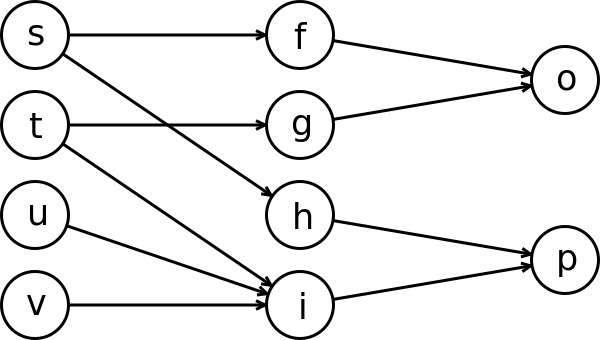
\includegraphics[scale=0.25]{intro_example}
\caption{
    Illustrative example of a dataset to which truth discovery can be applied
    with data sources $\{s, t, u, v\}$, facts $\{f, g, h, i\}$ and objects
    $\{o, p\}$
}
\label{td_fig_intro_example}
\end{figure}

For a simple example of a situation where trust can play an important role in
conflict resolution, consider the following example.

\begin{example}
\label{ex:intro_example}

Let $o$ and $p$ represent two images for which crowdsourcing workers are asked
to provide labels (in the truth discovery terminology, $o$ and $p$ are called
\emph{objects}). Consider workers (the data sources) $s, t, u$ and $v$ who put
forward potential labels $f, g$ for $o$, and $h, i$ for $p$, as shown in
\cref{td_fig_intro_example}; such potential answers are termed \emph{facts}. In the
graphical representation, sources, facts and objects are shown from left to
right, and the edges indicate claims made by sources and the objects to which
facts relate.

Without considering trust information, the label for $o$ appears a tie, with
both options $f$ and $g$ receiving one vote from sources $s$ and $t$
respectively.

Taking a trust-aware approach, however, we can look beyond object $o$ to
consider the \emph{trustworthiness} of $s$ and $t$. Indeed, when it comes to
object $p$, $t$ agrees with two extra sources $u$ and $v$, whereas $s$
disagrees with everyone. In principle there could be \emph{hundreds} of extra
sources here instead of just two, in which case the effect would be even more
striking. We may conclude that $s$ is \emph{less trustworthy} than $t$.
Returning to $o$, we see that $g$ is supported by a more trustworthy source,
and conclude that it should be accepted over $f$.

\end{example}

Many truth discovery algorithms have been proposed in the literature with a
wide range of techniques used, e.g. iterative heuristic-based
methods~\cite{pasternack2010,galland2010}, probabilistic models~\cite{yin2008},
maximum likelihood estimation and optimisation-based methods~\cite{li2016}, and
neural network
models~\cite{kotonya2020explainable,marshall2017neural,wang2018eann}. It is
common for such algorithms to be evaluated empirically by running them against
real-world or synthetic datasets for which the true facts are already known;
this allows \emph{accuracy} and other metrics to be calculated, and permits
comparison between algorithms (see \cite{waguih2014truth} for a systematic
empirical evaluation of this kind). This may be accompanied by some theoretical
analysis, such as calculating run-time complexity~\cite{gupta2011survey},
proving convergence of an iterative algorithm~\cite{yin_supervised_2011}, or
proving convergence to the `true' facts under certain assumptions on the
distribution of source
trustworthiness~\cite{xiao2016,xiao_thesis2018,ghosh_2011}.

A limitation of this kind of analysis is that the results only apply narrowly
to particular algorithms, due to the assumptions made (for instance, that
claims from sources follow a particular probability distribution). Such
assumptions can be problematic in domains where the desired truth is somewhat
`fuzzy'; for example, image classification problems and determining the
copyright status of
books.\footnote{\url{https://www.nytimes.com/2019/08/19/technology/amazon-orwell-1984.html}}

In this work we take first steps towards a more general approach, in which we
aim to study truth discovery
without reference to any specific methodology or probabilistic framework. To do
so we note the similarities between truth discovery and problems such as
judgment aggregation~\cite{endriss2016ja}, voting
theory~\cite{zwicker2016voting} ranking and recommendation
systems~\cite{altman2008,altman2005ranking,andersen2008,tennenholtz2004} in
which the \emph{axiomatic approach} of social choice has been successfully
applied.
%
In taking the axiomatic approach one aims to formulate \emph{axioms} that
encode intuitively desirable properties that an algorithm may possess. The
interaction between these axioms can then be studied; typical results include
\emph{impossibility results}, where it is shown that a set of axioms cannot
hold simultaneously, and \emph{characterisation results}, where it is shown
that a set of axioms are uniquely satisfied by a particular algorithm.

Such analysis brings a new \emph{normative} perspective to the truth discovery
literature. This complements empirical evaluation: in addition to seeing how well
an algorithm performs in practise on test datasets, one can check how well it
does against theoretical properties that any `reasonable' algorithm should
satisfy. The satisfaction (or failure) of such properties then shines new light
on the \emph{intuitive behaviour} of an algorithm, and may guide development of
new ones.

With this in mind, we develop a simplified framework for truth discovery in which
axioms can be formulated, and go on to give both an impossibility result and an
axiomatic characterisation of a baseline voting algorithm. We also analyse the
class of \emph{recursive} truth discovery algorithms, which includes many
existing examples from the literature. In particular, we analyse the well-known
algorithm \sums{}~\cite{pasternack2010} with respect to the axioms.

However, as a first step towards a social choice perspective of truth
discovery, our framework involves a number of simplifying assumptions not
commonly made in the truth discovery literature.

\begin{itemize}

    \item \textbf{Manipulation and collusion.} Some of our axioms assume
          sources are not \emph{manipulative}: they provide claims in good
          faith, and do not aim to misinform or artificially improve their
          standing with respect to the truth discovery algorithm. We also
          assume sources act independently, i.e. they do not \emph{collude}
          with or \emph{copy} one another.

    \item \textbf{Object correlations.} We do not model correlations between
          the objects of interest in the truth discovery problem. For example,
          in a crowdsourcing setting it may be known in advance that two
          objects $o$ and $p$ are similar, so that the true labels for
          $o$ and $p$ are correlated; this cannot be expressed in our
          framework.

    \item \textbf{Ordinal outputs.} For the most part, the outputs of our truth
          discovery methods consist of \emph{rankings} of the sources and
          facts. Thus, we describe when a source is considered \emph{more
          trustworthy} than another, but do not assign precise numerical values
          representing trustworthiness. This breaks with tradition in the truth
          discovery literature, but is a common point of view in social choice
          theory.

\end{itemize}

At first glance these are strong assumptions, and rule out potential
applications of our version of truth discovery. However, we argue that the
problem is non-trivial even in this simplified setting, and that interesting
axioms can still be put forth. The framework as set out here lays the
groundwork for these assumptions to be lifted in future work.

The paper is organised as follows. Our framework is introduced and formally
defined in the next section. \Cref{td_sec_specific_operators} provides examples of
truth discovery algorithms from the literature expressed in the framework. In
\cref{td_sec_axioms} we formally introduce the axioms and present an impossibility
result showing a subset of these cannot all be satisfied simultaneously. The
examples of \cref{td_sec_specific_operators} are then revisited in
\cref{td_sec_satisfaction_of_axioms}, where we analyse them with respect to the
axioms and propose modifications to resolve some axiom failures. In
\cref{td_sec_variable_domain} we extend the framework to allow variable domains of
sources, facts and objects, and give an impossibility result similar to that of
\cref{td_sec_axioms}. We discuss the axioms in \cref{td_sec_discussion} and related
work in \cref{td_sec_relatedwork}. We conclude
in \cref{td_sec_conclusion}. Missing proofs are given in \cref{chapter_td_proofs}.


\section{An idealised framework for truth discovery}
\label{td_sec_framework}

In this section we define our formal framework, which provides the key
definitions required for theoretical discussion and analysis of truth discovery
methods.

For most of the paper, we consider a fixed domain of finite and mutually
disjoint sets $\S$, $\F$ and $\O$ throughout, called the \emph{sources},
\emph{facts} and \emph{objects} respectively. All definitions and axioms will
be stated with respect to these sets.\footnote{We generalise to variable
domains in \cref{td_sec_variable_domain}.}

\subsection{Truth discovery networks}

A core definition of the framework is that of a \emph{truth discovery network},
which represents the input to a truth discovery problem. We model this as a
tripartite graph with certain constraints on its structure, in keeping with
approaches taken throughout the truth discovery
literature~\cite{yin2008,gupta2011survey}.

\begin{definition}
\label{def_td_network}
A \emph{truth discovery network} (hereafter a {\em TD network}) is a directed
graph $N = (V, E)$ where $V = \S \cup \F \cup \O$, and $E \subseteq (\S \times
\F) \cup (\F \times \O)$ has the following properties:

\begin{enumerate}
\item For each $f \in \F$ there is a unique $o \in \O$ with $(f, o) \in
E$, denoted $\obj_N(f)$. That is, each fact is associated with exactly one
object.

\item For $s \in \S$ and $o \in \O$, there is at most one directed path from
$s$ to $o$. That is, sources cannot claim multiple facts for a single object.

\item $(\S \times \F) \cap E$ is non-empty. That is, at least one claim is
made.

\end{enumerate}
We will say that $s$ \emph{claims} $f$ when $(s, f) \in E$. Let $\N$ denote the
set of all TD networks.
\end{definition}

\Cref{td_fig_intro_example} (page \pageref{td_fig_intro_example}) provides an example
of a TD network.  Note that there is no requirement that a source makes a claim
for \emph{every} object, or even that a source makes any claims at all. This
reflects the fact that truth discovery datasets are in practise extremely
sparse, i.e. each individual source makes few claims. Conversely, we allow for
facts that receive no claims from any sources.

Also note that the object associated with a fact $f$ is not fixed across all
networks. This is because we view facts as \emph{labels} for information that
sources may claim, not the pieces of information themselves. Similarly, we
consider objects simply as labels for real-world entities. Whilst a particular
piece of information has a fixed entity to which it pertains, the labels do
not.\footnotemark{}

\footnotetext{
    For example, when implementing truth discovery algorithms in practise it is
    common to assign integer IDs to the `facts' and `objects'; the algorithm
    then operates using only the integer IDs. In this case there is no reason
    to require that fact 17 is always associated with object 4, for example,
    and the same principle applies in our framework.
}

A special case of our framework is the binary case in which every object has
exactly two associated facts. This brings us close to the setting studied in
{\em judgment aggregation}~\cite{endriss2016ja} and, specifically (since
sources do not necessarily claim a fact associated to every object) to the
setting of {\em binary aggregation with
abstentions}~\cite{christoffbinary,dokow}. An important difference, however, is
that for simplicity we do not assume any {\em constraints} on the possible configurations of
true facts across \emph{different} objects. That is, any combination of facts
is feasible.  In judgment aggregation such an assumption has the effect of
neutralising the impossibility results that arise in that domain (see,
e.g.,~\cite{christoffbinary}). We shall see that that is not the case in our
setting.

To simplify the notation in what follows, for a network $N=(V, E)$ we write
$\facts_N(s) = \{f \in \F : (s, f) \in E\}$ for the set of facts claimed by a
source $s$, and $\src_N(f) = \{s \in \S : (s, f) \in E\}$ for the set of
sources claiming a fact $f$.

\subsection{Truth discovery operators}

Having defined the input to a truth discovery problem, the output must be
defined. Contrary to many approaches in the truth discovery literature which
output numeric \emph{trust scores} for sources and \emph{belief scores} for
facts~\cite{yin2008,pasternack2010,galland2010,zhi2015,zhang_robust_2016,zhang2018},
we consider the primary output to be \emph{rankings} of the sources and facts.
To the extent that we do consider numeric scores, it is only to induce a
ranking. This is because we are chiefly interested in \emph{ordinal properties}
rather than quantitative values. Indeed, for the theoretical analysis we wish
to perform it is only important that a source is \emph{more trustworthy} than
another; the particular numeric scores produced by an algorithm are irrelevant.

Moreover, the scores produced by existing algorithms may have no semantic
meaning~\cite{pasternack2010}, and so referring to numeric values is not
meaningful when comparing across algorithms. In this case it is only the
rankings of sources and facts that can be compared, which is further motivation
for our choice. This point of view is also common across the social choice
literature.

However, numerical scores do provide valuable information for comparing sources
and facts given a \emph{fixed} algorithm. For example, the magnitude of the
difference in trust scores for sources $s$ and $t$ tells us something about
\emph{confidence}: a small difference indicates low confidence in
distinguishing $s$ and $t$ -- even if one is ranked above the other -- whereas
a large difference indicates high confidence. In this sense our decision to
primarily deal with ordinal outputs (and ordinal axioms) is another simplifying
assumption compared to typical truth discovery settings.

For a set $X$, let $\orderings(X)$ denote the set of all total preorders on
$X$, i.e. the set of transitive, reflexive and complete binary relations on
$X$. We define a \emph{truth discovery operator} as a
function which maps networks to rankings of sources and facts.

\begin{definition}
\label{td_def_truth_discovery_operator}

An \emph{ordinal truth discovery operator} $T$ (hereafter {\em TD operator}) is
a mapping $T: \N \to \orderings(\S)
\times \orderings(\F)$. We shall write $T(N) = (\sle_N^T, \fle_N^T)$, i.e.
$\sle_N^T$ is a total preorder on $\S$ and $\fle_N^T$ is a total preorder on
$\F$.
\end{definition}

Intuitively, the relation $\sle_N^T$ is a measure of \emph{source
trustworthiness} in the network $N$ according to $T$, and $\fle_N^T$ is a
measure of \emph{fact believability}; $s_1 \sle_N^T s_2$ means that source
$s_2$ is \emph{at least as trustworthy} as source $s_1$, and $f_1 \fle_N^T f_2$
means fact $f_2$ is \emph{at least as believable} as fact $f_1$. The notation
$\slt_N^T$ and $\seq_N^T$ will be used to denote the strict and symmetric
orders induced by $\sle_N^T$ respectively. For fact rankings, $\flt_N^T$ and
$\feq_N^T$ are defined similarly.
%
Note that for simplicity the fact ranking $\fle_N^T$ compares \emph{all} facts,
even those associated with different objects in $N$.

To capture existing truth discovery methods we introduce \emph{numerical
operators}, which assign each source a numeric \emph{trust score} and each fact
a \emph{belief score}.

\begin{definition}
A \emph{numerical TD operator} is a mapping $T: \N \to \R^{\S \cup
\F}$, i.e. $T$ assigns to each TD network $N$ a
function $T(N) = T_N: \S \cup \F \to \R$.
For $s \in \S$, $T_N(s)$ is the \emph{trust score} for $s$ in the
network $N$ according to $T$; for $f \in \F$, $T_N(f)$ is the \emph{belief
score} for $f$. The set of all numerical TD operators will be denoted by
$\num$.

\end{definition}

Note that any numerical operator $T$ naturally induces an ordinal operator
$\hat{T}$, where ${s_1 \sle_N^{\hat{T}} s_2}$ iff ${T_N(s_1) \le T_N(s_2)}$, and
${f_1 \fle_N^{\hat{T}} f_2}$ iff ${T_N(f_1) \le T_N(f_2)}$. Henceforth we shall
write $\sle_N^T$, $\fle_N^T$ without explicitly defining the induced ordinal
operator $\hat{T}$.

It is worth noting that yet other truth discovery algorithms output neither
rankings nor numeric scores for facts, but only a single `true' fact for each
object~\cite{li2016,ding_finding_2016,yang_continuous_2018}. This is also the
approach taken in judgment aggregation, where an \emph{aggregation rule}
selects which formulas are to be taken as true. In the case of finitely many
possible facts, such algorithms can be modelled in our framework as numerical
operators where $T_N(f) = 1$ for each identified `true' fact $f$, and $T_N(g) =
0$ for other facts $g$. To go in the reverse direction and obtain the `true'
facts according to an operator, one may simply select the set of facts for each
object that rank maximally.

\section{Examples of truth discovery operators}
\label{td_sec_specific_operators}

Our framework can capture some operators that have
been proposed in the truth discovery literature. In this section we provide two
concrete examples: \voting{}, which is a simple approach commonly used as a
baseline method, and \sums{}~\cite{pasternack2010}. We go on to outline the
class of \emph{recursive operators} -- of which \sums{} is an instance -- which
contains many more examples from the literature.

\subsection{Voting}
\label{td_sec_voting}

In \voting{}, we consider each source to cast `votes' for the facts they claim,
and facts are ranked according to the number of votes received. Clearly this
method disregards the source trustworthiness aspect of truth discovery, as a
vote from one source carries as much weight as a vote from any other. As such,
\voting{} cannot be considered a serious contender for truth discovery. It is
nonetheless useful as a simple baseline method against which to compare more
sophisticated methods.

\begin{definition}
\voting{} is the numerical operator defined as follows: for any network $N \in
\N$, $s \in \S$ and $f \in \F$, $T_N(s) = 1$ and $T_N(f) = |\src_N(f)|$.
\end{definition}

Consider the network $N$ shown in \cref{td_fig_intro_example}. Facts $f,
g$ and $h$ each receive one vote, whereas $i$ receives 3. The fact ranking
induced by \voting{} is therefore $f \feq g \feq h \flt i$.
On the other hand, all sources receive a trust score of 1 and therefore rank
equally.

\subsection{Sums}
\label{td_sec_sums_example}

\sums{}~\cite{pasternack2010} is a simple and well-known operator adapted from
the \emph{Hubs and Authorities}~\cite{kleinberg1999} algorithm for ranking web
pages. The algorithm operates iteratively and recursively, assigning each
source and fact a sequences of scores, with the final scores taken as the limit
of the sequence.

Initially, scores are fixed at a constant value of $1/2$. The trust score for
each source is then updated by summing the belief score of its associated
facts. Similarly, belief scores are updated by summing the trust scores of the
associated sources. To prevent these scores from growing without bound as the
algorithm iterates, they are normalised at each iteration by dividing each
trust score by the maximum across all sources (belief scores are normalised
similarly).

Expressed in our framework, we have that if $T$ is the (numerical) operator
giving the scores at iteration $n$, then the pre-normalisation scores at
iteration $n+1$ are given by $T'$, where
\begin{equation}
\label{td_eqn_sums_defn}
    T'_N(s) = \sum_{f \in \facts_N(s)}{T_N(f)};
    \quad
    T'_N(f) = \sum_{s \in \src_N(f)}{T'_N(s)}
\end{equation}

Consider again the network $N$ shown in \cref{td_fig_intro_example}. It can be
shown that, with $T$ denoting the limiting scores from \sums{} with
normalisation, we have $T_N(s) = 0$, $T_N(t) = 1$, and $T_N(u) = T_N(v) =
\sqrt{2} / 2$. The induced ranking of sources is therefore $s \slt u \seq v
\slt t$.

For fact scores, we have $T_N(f) = 0$, $T_N(g) = \sqrt{2} - 1$,
$T_N(h) = 0$ and $T_N(i) = 1$, so the ranking is $f \feq h \flt g \flt i$. Note
that fact $g$ fares better under \sums{} than \voting{}, due to its association
with the highly-trusted source $t$.

\subsection{Recursive truth discovery operators}
\label{td_sec_recursive_truth_discovery_operators}

The iterative and recursive aspect of \sums{} is hoped to result in the desired
mutual dependence between trust and belief scores: namely that sources claiming
high-belief facts are seen as trustworthy, and vice versa. In fact, this
recursive approach is near universal across the truth discovery literature (see
for
instance~\cite{yang_probabilistic_2019,du2019,zhang2018,li2016,galland2010,zhi2015}).
As such it is appropriate to identify the class of \emph{recursive operators}
as an important subset of $\num$. To make a formal definition we first define
an \emph{iterative operator}.

\begin{definition}
An \emph{iterative operator} is a sequence $(T^n)_{n \in \Nat}$ of numerical
operators. An iterative operator is said to \emph{converge} to a numerical
operator $T^*$ if $\limn{T_N^n(z)}=T_N^*(z)$ for all networks $N$ and $z \in \S
\cup \F$. In such case the iterative operator can be identified with the
ordinal operator induced by its limit $T^*$.
\end{definition}

Note that it is possible that an iterative operator $(T^n)_{n \in \Nat}$
converges for only a subset of networks. In such case we can consider
$(T^n)_{n \in \Nat}$ to converge to a `partial operator' and identify it with
the induced partial ordinal operator; that is, a partial function $\N \to
\orderings(\S) \times \orderings(\F)$.
%
Recursive operators can now be defined as those iterative operators where
$T^{n+1}$ can be obtained from $T^n$.

\begin{definition}
An iterative operator $(T^n)_{n \in \Nat}$ is said to be \emph{recursive} if
there is a function $U: \num \to \num$ such that $T^{n+1} = U(T^n)$ for all $n
\in \Nat$.
\end{definition}

In this context the mapping $U: \num \to \num$ is called the \emph{update
function}, and the initial operator $T^1$ is called the \emph{prior operator}.
For a prior operator $T$ and update function $U$, we write $\rec(T, U)$ for the
associated recursive operator; that is, $T^1 = T$ and $T^{n+1}=U(T^n)$.

Returning to \sums{}, we see that \cref{td_eqn_sums_defn} defines a mapping $\num
\to \num$ and consequently an update function $U^{\text{Sums}}$. The
normalisation step can be considered a separate update function $\norm$ which
maps any numerical operator $T$ to $T'$, where\footnotemark
\[
    T_N'(s) = \frac{T_N(s)}{\max\limits_{x \in \S}{|T_N(x)|}}, \quad
    T_N'(f) = \frac{T_N(f)}{\max\limits_{y \in \F}{|T_N(y)|}}
\]
%
It can then be seen that \sums{} is the recursive operator
$\rec(T^{\text{fixed}},
\norm \circ U^{\text{Sums}})$, where $T^{\text{fixed}}_N \equiv 1/2$.

\footnotetext{
    If $\max_{x \in \S}{|T_N(x)|} = 0$ then the above is ill-defined; we set
    $T_N'(s) = 0$ for all $s$ in this case. Fact belief scores are defined
    similarly if the maximum is 0.
}

Many other existing algorithms proposed in the literature can also be realised
as recursive operators in the framework, such as \emph{Investment},
\emph{PooledInvestment}~\cite{pasternack2010},
\emph{TruthFinder}~\cite{yin2008}, LDT~\cite{zhang2018} and others.

\section{Axioms for truth discovery}
\label{td_sec_axioms}

Having laid out the formal framework, we now introduce axioms for truth
discovery. To start with, we consider axioms which encode a desirable
theoretical property that we believe any `reasonable' operator $T$ should
satisfy.
%
Several properties of this nature can be obtained by adapting existing
axioms from the social choice literature (e.g. from
voting~\cite{brandt2016introduction}, ranking
systems~\cite{tennenholtz2004,altman2008} and judgement
aggregation~\cite{endriss2016ja}), to our framework.

However, the correspondence between truth discovery and classical social choice
problems -- such as voting -- has its limits. To show this, we translate the
famous Independence of Irrelevant Alternatives (IIA) axiom~\cite{arrow1952} to
our setting, and argue that it is actually an \emph{undesirable} property.
Indeed, it will be seen that this translated axiom, in combination with two
basic desirable axioms, leads to \voting{}-like behaviour in every network,
which is undesirable for the reasons given in \cref{td_sec_voting}.
Furthermore, a slight strengthening of the IIA axiom completely characterises
the fact ranking component of \voting{}. These results formalise the intuition
that truth discovery's consideration of source-trustworthiness leads to
fundamental differences from classical social choice problems.

Afterwards, we will revisit the specific operators of the previous section to
check which axioms are satisfied.

\subsection{Coherence}

As mentioned previously, a guiding principle of truth discovery is that sources
claiming highly believed facts should be seen as trustworthy, and that facts
backed by highly trusted sources should be seen as believable.

Whilst this intuition is difficult to formalise in general, it is possible to
do so in particular cases where there are obvious means by which to compare the
set of facts for two sources (and vice versa). This situation is considered in
the axiomatic analysis of ranking and reputation systems under the name
\emph{Transitivity}~\cite{tennenholtz2004,altman2008}, and we adapt it to truth
discovery in this section. A preliminary definition is required.

\begin{definition}
\label{td_def_coherence_less_believable}

Let $T$ be a TD operator, $N$ be a TD network and $Y, Y' \subseteq \F$. We
say $Y$ is \emph{less believable} than $Y'$ with respect to $N$ and $T$
if there is a bijection $\phi: Y \to Y'$ such that $f \fle_N^T \phi(f)$ for
each $f \in Y$, and $\hat{f} \flt_N^T \phi(\hat{f})$ for some $\hat{f} \in Y$.

For $X, X' \subseteq \S$ we define $X$ \emph{less trustworthy} than $X'$ with
respect to $N$ and $T$ in a similar way.

\end{definition}

In plain English, $Y$ less believable than $Y'$ means that the facts in each
set can be paired up in such a way that each fact in $Y'$ is at least as
believable as its counterpart in $Y$, and at least one fact in $Y'$ is strictly
more believable. Now, consider a situation where $\facts_N(s_1)$ is less
believable than $\facts_N(s_2)$. In this case the intuition outlined above
tells us that $s_2$ provides `better' facts, and should thus be seen as more
trustworthy than $s_1$. A similar idea holds if $\src_N(f_1)$ is less
trustworthy than $\src_N(f_2)$ for some facts $f_1, f_2$. We state this
formally as our first axiom.

\begin{axiom}[Coherence]

For any network $N$, $\facts_N(s_1)$ less believable than $\facts_N(s_2)$
implies $s_1 \slt_N^T s_2$, and $\src_N(f_1)$ less trustworthy than
$\src_N(f_2)$ implies $f_1 \flt_N^T f_2$.

\end{axiom}

Coherence can be broken down into two sub-axioms: \emph{Source-Coherence},
where the first implication regarding source rankings is satisfied; and
\emph{Fact-Coherence}, where the second implication is satisfied. We take
Coherence to be a fundamental desirable axiom for TD operators.

\subsection{Symmetry}

Our next axiom requires that rankings of sources and facts should not depend on
their `names', but only on the structure of the network. To state it formally,
we need a notion of when two networks are essentially the same but use
different names.

\begin{definition}
Two TD networks $N$ and $N'$ are \emph{equivalent} if there is a
graph isomorphism $\pi$ between them that preserves sources, facts and objects,
i.e., $\pi(s) \in \S$, $\pi(f) \in \F$ and $\pi(o) \in \O$ for all $s \in \S$,
$f \in \F$ and $o \in \O$. In such case we write $\pi(N)$ for $N'$.
\end{definition}

\begin{axiom}[Symmetry]
Let $N$ and $N' = \pi(N)$ be equivalent networks. Then for all $s_1, s_2 \in
\S$, $f_1, f_2 \in \F$, we have
%\[
    $s_1 \sle_N^T s_2\ \textrm{iff } \pi(s_1) \sle_{N'}^T \pi(s_2)$
%\]
and
%\[
    $f_1 \fle_N^T f_2\ \textrm{iff } \pi(f_1) \fle_{N'}^T \pi(f_2)$.
%\]

\end{axiom}

In the theory of voting in social choice, Symmetry as above is expressed as two
axioms: \emph{Anonymity}, where output is insensitive to the names of voters,
and \emph{Neutrality}, where output is insensitive to the names of
alternatives~\cite{zwicker2016voting}. Analogous axioms are also used in
judgment aggregation.

Symmetry can also be broken down into sub-axioms where the above
need only hold for a subset of permutations $\pi$ satisfying some condition:
\emph{Source-Symmetry} (where $\pi$ must leave facts and objects fixed) and
\emph{Fact-Symmetry} (where $\pi$ leaves sources and objects fixed). For truth
discovery we have the additional notion of objects, and thus
\emph{Object-Symmetry} can defined be similarly.

% A related axiom in social choice is \emph{non-dictatorship}. Translated to
% truth discovery, this requires that there is no `dictator' source, whose
% claimed facts are taken as the most believable in \emph{any} network. One can
% show that a `dictatorial' operator cannot satisfy Symmetry; since any operator
% of interest does satisfy Symmetry, non-dictatorship will play no further role
% in our work.

\subsection{Fact ranking axioms}
\label{td_sec_fact_ranking_axioms}

Next, we introduce axioms that dictate the ranking of particular facts in cases
where there is an `obvious' ordering. \emph{Unanimity} and \emph{Groundedness}
express the idea that if all sources are in agreement about the status of a
fact, then an operator should respect this in its verdict. Two obvious ways in
which sources can be in agreement are when \emph{all} sources believe a fact is
true, and when \emph{none} believe a fact is true.

\begin{axiom}[Unanimity]
Suppose $N \in \N$, $f \in \F$, and $\src_N(f) = \S$. Then for any other $g \in
\F$, $g \fle_N^T f$.
\end{axiom}

\begin{axiom}[Groundedness]
Suppose $N \in \N$, $f \in \F$, and $\src_N(f) = \emptyset$. Then for any other
$g \in \F$, $f \fle_N^T g$.
\end{axiom}

That is, $f$ cannot do better than to be claimed by all sources when $T$
satisfies Unanimity, and cannot do worse than to be claimed by none when $T$
satisfies Groundedness.
%
Unanimity here is a truth discovery rendition of the same axiom in judgment
aggregation, and can also be compared to the \emph{weak Paretian} property in
voting~\cite{brandt2016introduction}. Groundedness is a version of the same
axiom studied in the analysis of collective annotation~\cite{kruger2014}.

The next axiom is a monotonicity property, which states that if $f$
receives extra support from a new source $s$, then its ranking should receive a
strictly positive boost.\footnote{One could also consider the weak version, in
which we only require $g \fle_{N'}^T f$ in the consequent; we discuss this in
\cref{td_sec_discussion}.} Note that we do not make any judgement on the new
ranking of $s$.

\begin{axiom}[Monotonicity]
Suppose $N \in \N$, $s \in \S$, $f \in \F \setminus \facts_N(s)$. Write
$E$ for the set of edges in $N$, and let $N'$ be the network in which $s$
claims $f$; i.e. the network with edge set
\[
    E' = \{(s, f)\} \cup E \setminus \{(s, g) : g \ne f, \obj_N(g) = \obj_N(f) \}
\]
Then for all $g \ne f$,
%\[
    $g \fle_N^T f\  \textrm{implies } g \flt_{N'}^T f$.
%\]
\end{axiom}

Note that the axioms in this section assume sources do not have `negative'
trust levels. That is, we assume that support from even the most untrustworthy
source still has a \emph{positive} effect on the believability of a fact.
Consequently, these axioms are not suitable in the presence of knowledgable but
malicious sources who always claim false facts. Indeed, otherwise a fact
claimed only by a `negative' source should rank strictly \emph{worse} than a
fact with no sources, but this goes against Groundedness. Similarly, receiving
extra support from a negative source should worsen a fact's ranking, contrary
to Monotonicity. Moreover, Monotonicity implicitly assumes sources act
independently, i.e. they do not \emph{collude} with one another.\footnote{Note
that collusion has been studied in the truth discovery literature (e.g.
\cite{dong2009integrating,balakrishnan2011sourcerank,dong_truth_2009}).}

While these assumptions may appear somewhat strong, we argue that this `simple'
case -- with no `negative' sources or collusion -- is already non-trivial and
permits interesting axiomatic analysis.
%
We therefore view Unanimity, Groundedness and Monotonicity as desirable
properties for TD operators.

\subsection{Independence axioms}
\label{td_sec_indep_axioms}

% AAMAS rebuttal:
%----------------
% We introduce POI to make a bridge to social choice, in which the IIA axiom
% (to which POI is our counterpart) occupies such a central place that it
% would be remiss of us to exclude it.
% The main purpose of Strong Independence is to give the characterisation of
% Voting. Intuitively we know Voting doesn't make sense, now we can say for
% sure *why* (i.e., because it forces Strong Independence).
% Overall the axioms are there to formalise the intuition behind the
% approach. It's important to write down formally what makes sense and what
% doesn't so that future researchers can proceed with clarity and certainty.

We now come to exploring the differences between truth discovery and other
social choice problems via \emph{independence} axioms. In voting,
this takes the form of Independence of Irrelevant Alternatives (IIA), which
requires that the ranking of two alternatives $A$ and $B$ depends only on the
individual assessments of $A$ and $B$, not on some `irrelevant' alternative
$C$.
% That is, if the voter preferences are changed such that the individual
% rankings of $A$ versus $B$ remain unchanged, the social ranking of $A$ and
% $B$ should remain unchanged.

% To translate this principle into an axiom for truth discovery, we need to
% decide which properties of a network $N$ should be considered relevant to the
% ranking of two facts (or two sources). There is no canonical choice here, since
% the role of objects is unique to truth discovery and can be handled in various
% ways.

% We start by considering the case where facts $f_1$, $f_2$ relate to the same
% object $o$. If one aims to construct an object-aware version of IIA, it is
% reasonable to suggest that only the other facts for $o$, and the sources
% claiming them, are relevant to the ranking of $f_1$ and $f_2$. This leads to
% the following axiom.

An analogous truth discovery axiom states that the ranking of facts $f_1$ and
$f_2$ for some object $o$ depends only on the claims relating to $o$.
Intuitively, this is \emph{not} a desirable property. Indeed, we have already
seen in \cref{ex:intro_example} that the claims for object $p$ in the
network from \cref{td_fig_intro_example} can play an important role in
determining the ranking of $f$ and $g$ for object $o$, but the adapted IIA
axiom precludes this.

This undesirability can be made precise. First, we must state the axiom
formally.

\begin{axiom}[Per-object Independence (POI)]

Let $o \in \O$. Suppose $N_1$, $N_2$ are networks such that $F_o =
\obj_{N_1}^{-1}(o) = \obj_{N_2}^{-1}(o)$ and $\src_{N_1}(f) = \src_{N_2}(f)$
for each $f \in F_o$. Then the restrictions of $\fle_{N_1}^T$ and
$\fle_{N_2}^T$ to $F_o$ are equal; that is, $f_1 \fle_{N_1}^T f_2\ \textrm{iff
}f_1 \fle_{N_2}^T f_2$ for all $f_1, f_2 \in F_o$.

\end{axiom}

Considering \cref{td_fig_intro_example} again, POI implies that the ranking
of $f$ and $g$ remains the same if the claims for $h$ and $i$ are removed. But
in this case, Symmetry implies $f \feq g$. Similarly, the ranking of $h$ and
$i$ remains the same if the claims for $f$ and $g$ are removed. In this case,
Symmetry together with Monotonicity implies $h \flt i$, since $|\src_N(h)| <
|\src_N(i)|$.

This observation forms the basis of the following result, which formalises the
undesirability of POI: in the presence of our less controversial requirements
of Symmetry and Monotonicity, it forces \voting{}-like behaviour within
$\obj_N^{-1}(o)$ for each $o \in \O$.  We note that, for the special case of
binary networks, similar results have been shown in the literature on binary
aggregation with abstentions~\cite{christoffbinary}.

\begin{theorem}
\label{td_thm_poi_voting}
Let $T$ be any operator satisfying Symmetry, Monotonicity and POI. Then for any
$N \in \N$, $o \in \O$ and $f_1, f_2 \in \obj_N^{-1}(o)$ we have $f_1 \fle_N^T
f_2$ iff $|\src_N(f_1)| \le |\src_N(f_2)|$.
\end{theorem}

\begin{proof}[Proof (sketch)]
% \begin{proof}[Proof (sketch)]

We will sketch the main ideas of the proof here with some technical details
omitted; see \cref{chapter_td_proofs} for the full proof. Let $N$ be a
network, $o$ be an object and $f_1, f_2 \in \obj_N^{-1}(o)$. Consider $N'$
obtained by removing from $N$ all claims for objects other than $o$. By POI, we
have $f_1 \fle_N^T f_2$ iff $f_1 \fle_{N'}^T f_2$.  Since $|\src_N(f_j)| =
|\src_{N'}(f_j)|$ also ($j \in \{1,2\}$), it is sufficient for the proof to
show that $f_1 \fle_{N'}^T f_2$ iff $|\src_{N'}(f_1)| \le |\src_{N'}(f_2)|$.

For the `if' direction, first suppose $|\src_{N'}(f_1)| = |\src_{N'}(f_2)|$.
Let $\pi$ be the permutation which swaps $f_1$ with $f_2$ and swaps each source
in $\src_{N'}(f_1)$ with one in $\src_{N'}(f_2)$; then we have $\pi(N') = N'$,
and Symmetry of $T$ gives $f_1 \feq_{N'}^T f_2$. In particular $f_1 \fle_{N'}^T
f_2$ as required.

Otherwise, $|\src_{N'}(f_2)| - |\src_{N'}(f_1)| = k > 0$. Consider $N''$ where
$k$ sources from $\src_{N'}(f_2)$ are removed, and all other claims remain. By
Symmetry as above, $f_1 \feq_{N''}^T f_2$. Applying Monotonicity $k$ times we
can produce $N'$ from $N''$ and get $f_1 \flt_{N'}^T f_2$ as desired.

For the `only if' statement, suppose $f_1 \fle_{N'}^T f_2$ but, for
contradiction, $|\src_{N'}(f_1)| > |\src_{N'}(f_2)|$. Applying Monotonicity
again as above we get $f_1 \fgt_{N'}^T f_2$ and the required contradiction.
\end{proof}

Recall that Coherence formalises the idea that source-trustworthiness should
inform the fact ranking, and vice versa. Clearly \voting{} does not conform to
this idea, and in fact even the object-wise voting patterns in
\cref{td_thm_poi_voting} are incompatible with Coherence. This can easily be seen
in the network in \cref{td_fig_intro_example} where, regarding object $p$, we have
$|\src_N(h)| < |\src_N(i)|$ (hence $h \flt^T_N i$) and, regarding object $o$,
we have $|\src_N(f)| = |\src_N(g)|$ (hence $f \feq^T_N g$). Hence $\facts_N(s)$
is less believable than $\facts_N(t)$. If Coherence held this would give $s
\slt_N^T t$, but then $\src_N(f)$ is less trustworthy than $\src_N(g)$, giving
$f \flt_N^T g$ -- a contradiction. From this discussion and
\cref{td_thm_poi_voting} we obtain as a corollary the following first
impossibility result for truth discovery.

\begin{theorem}
\label{td_thm_impossibility}
There is no TD operator satisfying Coherence, Symmetry, Monotonicity and POI.
\end{theorem}

Given that \cref{td_thm_poi_voting} characterises the fact ranking of
\voting{} for facts relating to a single object, it is natural to ask if there
is a stronger form of independence that guarantees this behaviour across
\emph{all} facts. As our next result shows, the answer is \emph{yes}, and the
necessary axiom is obtained by ignoring the role of objects altogether for fact
ranking.

\begin{axiom}[Strong Independence]
For any networks $N_1, N_2$ and facts $f_1, f_2$, if $\src_{N_1}(f_j) =
\src_{N_2}(f_j)$ for each $j \in \{1, 2\}$ then $f_1 \fle_{N_1}^T f_2$ iff
$f_1 \fle_{N_2}^T f_2$.
\end{axiom}

That is, the ranking of two facts $f_1$ and $f_2$ is determined solely by the
sources claiming $f_1$ and $f_2$. In particular, the fact-object affiliations
and claims for facts other than $f_1, f_2$ are irrelevant when deciding on
$f_1$ versus $f_2$. Note that Strong Independence implies POI.
%
We have the following result.

\begin{theorem}
\label{td_thm_voting_characterisation}
Suppose $|\O| \ge 3$. Then an operator $T$ satisfies Strong Independence,
Monotonicity and Symmetry if and only if for any network $N$ and $f_1, f_2 \in
\F$ we have
\[
    f_1 \fle_N^T f_2 \iff |\src_N(f_1)| \le |\src_N(f_2)|
\]
\end{theorem}

\Cref{td_thm_voting_characterisation} can be seen as a characterisation of the
class of TD operators that rank facts in the same way as \voting{}. The proof
is similar to that of \cref{td_thm_poi_voting}, but uses a different
transformation to obtain a modified network $N'$ in the first step.

We have established that neither POI nor Strong Independence are satisfactory
axioms for truth discovery, and a weaker independence property is required.
\Cref{td_fig_intro_example} can help us once again in this regard. Whereas POI and
Strong Independence would say that facts $h$ and $i$ are irrelevant to $f$, the
argument with Coherence for \cref{td_thm_impossibility} suggests otherwise due the
indirect links via the sources. We therefore propose that only when there is no
(undirected) path between two nodes can we consider them to be truly irrelevant
to each other. That is, nodes are relevant to each other iff they lie in the
same \emph{connected component} of the network.

% We define connected components for TD networks as follows. For a
% network $N$, define an equivalence relation $\sim_N$ on $\S \cup \F \cup \O$ by
% $z_1 \sim_N z_2$ iff there is a path in $N$ from $z_1$ to $z_2$, ignoring the
% directions of edges. The connected components of $N$ are the (directed) induced
% subgraphs of the equivalence classes of $\sim_N$. In what follows, we abuse
% notation by identifying a connected component $G$ with the set of nodes
% contained in it.

Our final rendering of independence states that the ordering of two facts in
the same connected component does not depend on any claims outside of the
component, and similarly for sources.

\begin{axiom}[Per-component Independence (PCI)]
For any TD networks $N_1$, $N_2$ with a common connected component
$G$, the restrictions of $\sle_{N_1}^T$ and $\sle_{N_2}^T$ to $G \cap \S$ are
equal, and the restrictions of $\fle_{N_1}^T$ and $\fle_{N_2}^T$ to $G \cap \F$
are equal; that is,
%\[
    $s_1 \sle_{N_1}^T s_2\ \textrm{iff } s_1 \sle_{N_2}^T s_2$
%\]
and
%\[
    $f_1 \fle_{N_1}^T f_2\ \textrm{iff } f_1 \fle_{N_2}^T f_2$
%\]
for $s_1, s_2 \in G \cap \S$ and $f_1, f_2 \in G \cap \F$.

\end{axiom}

In analogy with Source/Fact Coherence and Source/Fact Symmetry, it is possible
to split the two requirements of PCI into sub-axioms Source-PCI (in which only
the constraint on source ranking is imposed) and Fact-PCI (in which only the
fact ranking is constrained).

Note that while our framework can be easily adapted to require \emph{by
definition} that a network is itself connected (and therefore has only one
connected component), we have found that datasets with multiple connected
components do indeed occur in practise.\footnotemark{} This means that failure
of PCI is a real issue, and consequently we consider PCI to be another core
axiom that all reasonable operators should satisfy.

\footnotetext{
    For example, the \emph{Book} and \emph{Restaurant} datasets found at the
    following web page each contain two connected components:
    \url{http://lunadong.com/fusionDataSets.htm}
}

\section{Satisfaction of the axioms}
\label{td_sec_satisfaction_of_axioms}

With the axioms formally defined, we can now consider whether they are
satisfied by the example operators of \cref{td_sec_specific_operators}.
\voting{} can be analysed outright; for \sums{} we require some preliminary
results giving sufficient conditions for iterative and recursive operators to
satisfy various axioms. It will be seen that neither \voting{} nor \sums{}
satisfy all our desirable axioms, but it is possible to modify each operator to
gain some improvement with respect to the axioms.

\subsection{Voting}

As the simplest operator, we consider \voting{} first. The following
theorem shows that all axioms except Coherence are satisfied. Since Coherence
is a fundamental principle of truth discovery, and we actually consider POI and
Strong Independence to be \emph{undesirable}, this formally rules out \voting{} as a
viable operator.

\begin{theorem}
\label{td_thm_voting_axioms}
\voting{} satisfies Symmetry, Unanimity, Groundedness, Monotonicity, POI, Strong
Independence and PCI. \voting{} does not satisfy Coherence.
\end{theorem}

The proof is straightforward, and is deferred to \cref{chapter_td_proofs}.  Note that
once Symmetry, Monotonicity and POI are shown, the fact that \voting{} fails
Coherence follows from our impossibility result (\cref{td_thm_impossibility}), and
\cref{td_fig_intro_example} serves as an explicit counterexample.

\subsection{Iterative and recursive operators}
\label{td_sec_axioms_for_iterative_and_recursive_operators}

In this section we give sufficient conditions for iterative and recursive
operators to satisfy various axioms. These results will be useful in what
follows when analysing \sums{}, although they may also be applied more
generally to other operators.

\paragraph{Coherence.}

To analyse whether the limit of a recursive operator satisfies Coherence, we
consider how the update function $U$ behaves when the difference in belief
scores between the facts of $s_1$ and $s_2$ is `small' (and similarly for the
sources of $f_1$, $f_2$). To that end, we introduce a numerical variant of a
set of facts $Y$ being `less believable' than $Y'$.

\begin{definition}
\label{td_def_num_less_believable}

Let $T$ be a numerical TD operator, $N$ a network, $Y, Y' \subseteq \F$ and
$\epsilon, \rho > 0$.  We say $Y$ is \emph{$(\epsilon, \rho)$-less believable}
than $Y'$ with respect to $N$ and $T$ if there is a bijection $\phi: Y \to Y'$
such that $T_N(f) - T_N(\phi(f)) \le \epsilon$ for all $f \in Y$, and
$T_N(\hat{f})
- T_N(\phi(\hat{f})) \le \epsilon - \rho$ for some $\hat{f} \in Y$.

For $X, X' \subseteq \S$, we define $X$ \emph{$(\epsilon, \rho)$-less
trustworthy} than $X'$ similarly.

\end{definition}

This generalises \cref{td_def_coherence_less_believable} by relaxing the
requirement that ${f \fle_N^T \phi(f)}$, and instead requiring that $f$ can
only be more believable than $\phi(f)$ by some threshold $\epsilon > 0$.
\Cref{td_def_coherence_less_believable} is recovered in the limiting
case $\epsilon \to 0$. We obtain a sufficient condition on the update function
$U$ for a recursive operator to satisfy Source-Coherence.

\begin{lemma}
\label{td_lemma_source_coherence_lemma}

Let $U: \num \to \num$. For any prior operator $T^{\text{prior}}$,
$\rec(T^{\text{prior}}, U)$ satisfies Source-Coherence if the following
condition is satisfied: there exist $C, D > 0$ such that for all networks $N$
and numerical operators $T$ it holds that if $\facts_N(s_1)$ is $(\epsilon,
\rho)$-less believable than $\facts_N(s_2)$ with respect to $N$ and $T$, then
%\[
    $T'_N(s_1) - T'_N(s_2) \le C\epsilon - D\rho$,
%\]
where $T' = U(T)$.

\end{lemma}

The proof of \cref{td_lemma_source_coherence_lemma} uses the following
result, the proof of which is a straightforward application of the definition
of the limit.

\begin{lemma}
\label{td_lemma_ordering_epsilon_lemma}
Let $N$ be a truth discovery network and $(T^n)_{n \in \Nat}$ be a convergent
iterative operator with limit $T^*$. Then for $f_1, f_2 \in \F$, $f_1 \fle_N^{T^*} f_2$
if and only if
\[
    \forall \epsilon > 0\ \exists K \in \Nat : \forall n \ge K:
        T_N^n(f_1) - T_N^n(f_2) \le \epsilon
\]
Also, $f_1 \flt_N^{T^*} f_2$ if and only if
\[
    \exists \rho > 0 : \forall \epsilon > 0\ \exists K \in \Nat : \forall n \ge K:
        T_N^n(f_1) - T_N^n(f_2) \le \epsilon - \rho
\]
Analogous statements for source rankings also hold.
\end{lemma}

\begin{proof}[Proof of \cref{td_lemma_source_coherence_lemma}]

Let $N$ be a network. Suppose $U$ has the stated property and that
$\rec(T^{\text{prior}}, U) = (T^n)_{n \in \Nat}$ converges to $T^*$. Suppose
$\facts_N(s_1)$ is less trustworthy than $\facts_N(s_2)$ with respect to $N$
and $T^*$ under a bijection $\phi$. We must show that $s_1 \slt_N^{T^*} s_2$.

Now, there is some $\hat{f} \in \facts_N(s_1)$ with $\hat{f} \flt_N^{T^*}
\phi(\hat{f})$. The second part of \cref{td_lemma_ordering_epsilon_lemma}
therefore applies; let $\rho$ be as given there. Now let $\epsilon > 0$.
Since $f \fle_N^{T^*} \phi(f)$ for each $f \in \facts_N(s_1)$, we may apply
\cref{td_lemma_ordering_epsilon_lemma} with $f, \phi(f)$ and
$\bar{\epsilon} = \epsilon / C$ to get that there is $K \in \Nat$ such that
\[
    T_N^n(f) - T_N^n(\phi(f)) \le \bar{\epsilon}
\]
and
\[
    T_N^n(\hat{f}) - T_N^n(\phi(\hat{f})) \le \bar{\epsilon} - \rho
\]
for all $n \ge K$. In other words, $\facts_N(s_1)$ is $(\bar{\epsilon},
\rho)$-less believable than $\facts_N(s_2)$ with respect to $N$ and $T^n$ for
all $n \ge K$.

Now, recall that $T^{n+1}=U(T^n)$. For $m \ge K' = K + 1$ we therefore have,
applying our condition on $U$,
\[
    T_N^m(s_1) - T_N^m(s_2) \le C\bar{\epsilon} - D\rho
    = \epsilon - D\rho
\]
Since $D\rho$ is positive and does not depend on $\epsilon$, we get $s_1
\slt_N^{T^*} s_2$ by \cref{td_lemma_ordering_epsilon_lemma}. This shows that
$T^*$ satisfies Source-Coherence.
\end{proof}

A similar result gives conditions under which Fact-Coherence is satisfied.

\begin{lemma}
\label{td_lemma_fact_coherence_lemma}

$\rec(T^{\text{prior}}, U)$ satisfies Fact-Coherence if there exist $E, F > 0$
such that for all networks $N$ and numerical operators $T$ it holds that if
$\src_N(f_1)$ is $(\epsilon, \rho)$-less trustworthy than $\src_N(f_2)$ with
respect to $N$ and $T'$, then
%\[
    $T'_N(f_1) - T'_N(f_2) \le E\epsilon - F\rho$,
%\]
where $T' = U(T)$.

\end{lemma}

\begin{proof}
The proof proceeds in an identical way to \cref{td_lemma_source_coherence_lemma};
the only difference is that we may simply
take $K' = K$ in the final step.
\end{proof}

Note that there is asymmetry between \cref{td_lemma_source_coherence_lemma}
and \cref{td_lemma_fact_coherence_lemma} -- in the condition on $U$ in
\cref{td_lemma_source_coherence_lemma} we have $\facts_N(s_1)$ $(\epsilon,
\rho)$-less trustworthy than $\facts_N(s_2)$ with respect to $T$, whereas in
\cref{td_lemma_fact_coherence_lemma} the corresponding condition is with
respect to $T' = U(T)$. This reflects the manner in which \sums{} and other TD
operators are typically defined: source trust scores are updated based on the
fact scores of the previous iteration, whereas fact belief scores are updated
based on the (new) trust scores in the \emph{current} iteration.

Also note that the above results still hold if $U$ has the stated property only
for `small' $\epsilon$; that is, if there is a constant $0 < \lambda < 1$ such
that the property holds for all $\rho$ and for all $\epsilon < \lambda\rho$.

\paragraph{Symmetry and PCI.} When considering either Symmetry or PCI
for an iterative operator $(T^n)_{n \in \Nat}$, it is not enough to know that
each $T^n$ satisfies the relevant axiom. The following example illustrates this
fact for Symmetry.

\begin{example}
Fix some $\hat{f} \in \F$, and define an iterative operator by
\[
    T_N^n(s) = 1
\]
\[
    T_N^n(f) = \begin{cases}
        |\src_N(f)| + (1 - \frac{1}{n + 1}) & \text{ if } |\src_N(f)| = |\src_N(\hat{f})| \\
        |\src_N(f)| & \text{ otherwise }
    \end{cases}
\]
That is, each $T^n$ is a modification of \voting{} in which we boost the score
of all facts tied with $\hat{f}$ under \voting{} by $1 - \frac{1}{n+1}$.
Since this additional weight is (strictly) less than 1 for each $n$, the
ordinal operator induced by $T^n$ is simply \voting{}, and therefore satisfies
Symmetry. However, it is easy to see that the limit operator $T^*$ has
$T_N^*(\hat{f}) = |\src_N(\hat{f})| + 1$; this means $T^*$ uses extra
information beyond the structure of the network $N$ in its ranking (namely, the
identity of a selected fact $\hat{f}$) which violates Symmetry.

\end{example}

Using a similar tactic, one can construct a sequence of numerical operators
$(T^n)_{n \in \Nat}$ such that each $T^n$ satisfies PCI, but the limit operator
$T^*$ does not.

Fortunately, there is a natural strengthening of both Symmetry and PCI for
numerical operators which \emph{is} preserved in the limit. Let us say that a
numerical operator $T$ satisfies \emph{numerical Symmetry} if for any
equivalent networks $N, \pi(N)$ we have $T_N(z) = T_{\pi(N)}(\pi(z))$ for all
$z \in \S \cup \F$. Similarly, $T$ satisfies \emph{numerical PCI} if for any
networks $N_1$ and $N_2$ with a common connected component $G$, we have
$T_{N_1}(z) = T_{N_2}(z)$ for all $z \in G \cap (\S \cup \F)$. Clearly
numerical Symmetry implies Symmetry, and numerical PCI implies PCI. The
following result is immediate.

\begin{lemma}
    \label{td_lemma_ns_npci_preservation}
    Suppose $(T^n)_{n \in \Nat}$ converges to $T^*$. Then
    \begin{itemize}
        \item If $T^n$ satisfies numerical Symmetry for each $n \in \Nat$, then
              $T^*$ satisfies Symmetry.
        \item If $T^n$ satisfies numerical PCI for each $n \in \Nat$, then
              $T^*$ satisfies PCI.
    \end{itemize}
\end{lemma}

As a consequence of \cref{td_lemma_ns_npci_preservation}, any recursive
operator $\rec(T^\text{prior}, U)$ satisfies Symmetry whenever
$T^{\text{prior}}$ satisfies numerical Symmetry and $U$ \emph{preserves}
numerical Symmetry, in the sense that $U(T)$ satisfies numerical Symmetry
whenever $T$ does (and similarly for PCI).

\paragraph{Unanimity, Groundedness and Monotonicity.} In contrast to Symmetry
and PCI, both Unanimity and Groundedness \emph{are} preserved when taking the
limit of an iterative operator.

\begin{lemma}
    \label{td_lemma_unam_groundedness_preservation}
    Suppose $(T^n)_{n \in \Nat}$ converges to $T^*$. Then

    \begin{itemize}
        \item If $T^n$ satisfies Unanimity for each $n \in \Nat$, then $T^*$
              satisfies Unanimity.
        \item If $T^n$ satisfies Groundedness for each $n \in \Nat$, then $T^*$
              satisfies Groundedness.
    \end{itemize}
\end{lemma}

For Monotonicity, we require the following (stronger) property to hold for each
$T^n$.

\begin{definition}

    A numerical operator $T$ satisfies \emph{Improvement} if for each $N, N'$
    and $f$ as in the statement of Monotonicity, we have $\delta(f) >
    \delta(g)$ for all $g \ne f$, where
    \[
        \delta(g) = T_{N'}(g) - T_N(g)
    \]
    In this case we write $\rho_{N,N'} = \min_{g \ne f}{(\delta(f) -
    \delta(g))} > 0$.

\end{definition}

Here $\delta(g)$ is the amount by which the belief score for $g$ increases when
going from the network $N$ to $N'$. Improvement simply says that when adding a
new source to a fact $f$, it is $f$ that sees the largest increase.

\begin{proposition}

    Suppose $(T^n)_{n \in \Nat}$ converges to $T^*$, and $T^n$ satisfies
    Improvement for each $n \in \Nat$. Suppose also that $\inf_{n \in
    \Nat}{\rho_{N,N'}^n} > 0$ for each $N, N'$ arising in the statement of
    Monotonicity. Then $T^*$ satisfies Monotonicity.

\end{proposition}

\begin{proof}

    Let $N, N'$ and $f$ be as in the statement of Monotonicity, and suppose $g
    \fle_N^{T^*} f$ for some $g \ne f$. We will show $g \flt_{N'}^{T^*} f$
    using \cref{td_lemma_ordering_epsilon_lemma}.

    Write $\rho^* = \inf_{n \in \Nat}{\rho_{N,N'}^n} > 0$ and let $\epsilon >
    0$. Since $g \fle_N^{T^*} f$, there is $K \in \Nat$ such that $T^n_N(g) -
    T^n_N(f) \le \epsilon$ for all $n \ge K$. For such $n$, we have
    \begin{align*}
        T_{N'}^n(g) - T_{N'}^n(f)
        &= (T_N^n(g) + \delta^n(g)) - (T_N^n(f) + \delta^n(f)) \\
        &=
            \underbrace{T_N^n(g) - T_N^n(f)}_{\le \epsilon}
            -
            \underbrace{(\delta^n(f) - \delta^n(g))}_{\ge \rho_{N,N'}^n}
            \\
        &\le \epsilon - \rho_{N,N'}^n \\
        &\le \epsilon - \rho^*
    \end{align*}
    By \cref{td_lemma_ordering_epsilon_lemma}, we have $g \flt_{N'}^{T^*} f$
    as required.
\end{proof}

The requirement that $\inf_{n \in \Nat}{\rho_{N,N'}^n} > 0$ is a technical
condition which ensures the \emph{strict} inequality $g \flt_{N'}^{T^*} f$
holds in the limit, as required for Monotonicity. If this condition fails $T^*$
still satisfies a natural `weak Monotonicity' axiom, in which the strict
inequality $g \flt_{N'}^{T^*} f$ is replaced with $g \fle_{N'}^{T^*} f$.

\subsection{Sums}

We come to the axiomatic analysis of \sums{}. Coherence and the simpler axioms
are satisfied here, and the undesirable independence axioms (POI and Strong
Independence) are not. However, Monotonicity and PCI do \emph{not} hold. Since
PCI is one of our most important axioms that we expect any reasonable operator
to satisfy, this potentially limits the usefulness of \sums{} in practise.

\begin{theorem}
\label{td_thm_sums_axioms}
\sums{} satisfies Coherence, Symmetry, Unanimity and Groundedness. \sums{} does
not satisfy POI, Strong Independence, PCI or Monotonicity.
\end{theorem}

\begin{proof}[Proof (sketch)]
% \begin{proof}[Proof (sketch)]

Symmetry, Unanimity and Groundedness can be easily shown from
\cref{td_lemma_ns_npci_preservation} and
\cref{td_lemma_unam_groundedness_preservation}; the details can be found in the
appendix.
%
In the remainder of the proof, $(T^n)_{n \in \Nat}$ will denote the iterative
operator \sums{}, $T^*$ will denote the limit operator, and $U = \norm \circ
U^{\text{Sums}}$ will denote the update function for \sums{}.

\paragraph{Coherence.} We will show Source-Coherence using
\cref{td_lemma_source_coherence_lemma}. The argument for Fact-Coherence is similar
(using \cref{td_lemma_fact_coherence_lemma}) and can be found in the appendix.

Suppose $N \in \N$, $T \in \num$, $\epsilon, \rho > 0$, and $\facts_N(s_1)$ is
$(\epsilon, \rho)$-less believable than $\facts_N(s_2)$ with respect to $N$ and
$T$ under a bijection $\phi: \facts_N(s_1) \to \facts_N(s_2)$. By definition
there is $\hat{f} \in \facts_N(s_1)$ such that $T_N(\hat{f}) -
T_N(\phi(\hat{f})) \le \epsilon - \rho$. By the remark after the proof of
\cref{td_lemma_source_coherence_lemma}, we may assume without loss of generality
that $\epsilon < \frac{1}{|\F|} \rho$.

Recall that the update function for \sums{} is $U = \norm \circ
U^{\text{Sums}}$. Write $T' = U^{\text{Sums}}(T)$ and $\tilde{T} = U(T)
= \norm(U^{\text{Sums}}(T))$ so that $\tilde{T} = \norm(T')$. We must show that
$\tilde{T}_N(s_1) - \tilde{T}_N(s_2) \le C\epsilon - D\rho$ for some constants
$C, D > 0$.

Note at this stage that it is possible to further weaken the hypotheses of
\cref{td_lemma_source_coherence_lemma}: the result follows if $U$ has the
stated property not for \emph{all} operators $T$, but only for those such that
$T = T^n$ for some $n \in \Nat$. Next, note that if $T'_N(x) = 0$ for all $x
\in \S$ then trust and belief scores are 0 in all subsequent iterations, and
thus all sources rank equally in the limit $T^*$.  But this means the
hypothesis for Source-Coherence cannot be satisfied (there are no strict
inequalities). We may therefore assume without loss of generality that $T'_N(x)
\ne 0$ for at least one $x \in \S$. Therefore, by definition of $\norm$,
\[
    \tilde{T}_N(s) = \alpha T'_N(s)
\]
where
\[
    \alpha = \frac{1}{\max\limits_{x \in \S}{|T'_N(x)|}}
\]
Applying the definition of $U^{\text{Sums}}$ and using the pairing of $\facts_N(s_1)$
and $\facts_N(s_2)$ via $\phi$, we have
\begin{align*}
    \tilde{T}_N(s_1) - \tilde{T}_n(s_2)
    &= \alpha[T'_N(s_1) - T'_N(s_2)] \\
    &= \alpha \left[
        \sum_{f \in \facts_N(s_1)}{T_N(f)}
        -
        \sum_{f \in \facts_N(s_1)}{T_N(\phi(f))}
    \right] \\
    &= \alpha
        \sum_{f \in \facts_N(s_1)}{
            \Big(
                T_N(f) - T_N(\phi(f))
            \Big)
        } \\
    &= \underbrace{\alpha}_{> 0}
       \left[
        \underbrace{
            \Big(
                T_N(\hat{f}) - T_N(\phi(\hat{f}))
            \Big)
        }_{\le \epsilon - \rho}
        +
        \sum_{f \in \facts_N(s_1) \setminus \{\hat{f}\} }{
            \underbrace{
                \Big(
                    T_N(f) - T_N(\phi(f))
                \Big)
            }_{\le \epsilon}
        }
    \right] \\
    & \le \alpha
       \left[
        \epsilon - \rho
        +
        \sum_{f \in \facts_N(s_1) \setminus \{\hat{f}\} }{
            \epsilon
        }
    \right] \\
    & \le \alpha
      \cdot
      \underbrace{
        \Big(|\F|\epsilon - \rho\Big)
      }_{< 0}
\end{align*}
To complete the proof, we need to find a lower bound for $\alpha$ that is
independent of $T$ and $N$ (note that a \emph{lower} bound on $\alpha$ is
required since $|\F|\epsilon - \rho$ is negative). It is here that we use the
assumption that $T = T^n$ for some $n \in \Nat$. Since $T^n_N(x) \in [0,1]$ for
any $n \in \Nat$ and $x \in S$, we have
\[
    |T_N'(x)|
    = T_N'(x)
    = \sum_{f \in \facts_N(x)}{
           \underbrace{T_N(f)}_{\le 1}
       }
     \le |\facts_N(x)|
     \le |\F|
\]
and so
\[
    \alpha
    = \frac{1}{\max\limits_{x \in \S}{|T'_N(x)|}}
    \ge \frac{1}{|\F|}
\]
Combining this with the above bound for $\tilde{T}_N(s_1) - \tilde{T}_n(s_2)$,
we get
\[
    \tilde{T}_N(s_1) - \tilde{T}_n(s_2)
    \le
    \frac{1}{|\F|} \Big(
        |\F|\epsilon - \rho
    \Big)
    = \epsilon - \frac{1}{|\F|}\rho
\]
Taking $C = 1$ and $D = \frac{1}{|\F|}$, the hypotheses of
\cref{td_lemma_source_coherence_lemma} are satisfied; thus \sums{} satisfies
Source-Coherence.

\paragraph{POI, Strong Independence, PCI and Monotonicity.}

The remaining axioms are handled by counterexamples derived from the network
shown in \cref{td_fig_sums_indep_poi_counterexample}. It can be shown that, if $N$
denotes this network, we have $T_N^*(f) = T_N^*(g) = 0$, so $f \feq_N^{T^*} g$.

Let $N'$ denote the network whose claims are just those of the top connected
component. Then it can be shown that $T_{N'}^*(f) = 1$ and $T_{N'}^*(g) = 0$,
i.e.  $g \flt_{N'}^{T^*} f$.  However it is easily verified that our three
independence axioms, if satisfied, would each imply $f \fle_N^{T^*} g$ iff $f
\fle_{N'}^{T^*} g$. Therefore none of POI, Strong Independence and PCI can
hold for \sums{}.

For Monotonicity, consider the network $N''$ obtained from $N$ by removing the
edge $(u, g)$. Then we still have $T_{N''}^*(f) = T_{N''}^*(g) = 0$, and in
particular $f \fle_{N''}^{T^*} g$. Returning to $N$ amounts to adding extra
support for the fact $g$. Monotonicity would give $f \flt_N^{T^*} g$ here, but
this is clearly false. Hence Monotonicity is not satisfied by \sums{}.

\begin{figure}[ht]
\centering
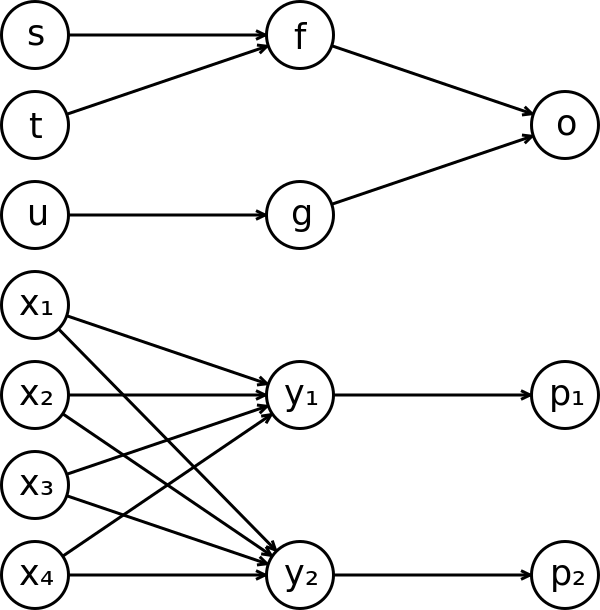
\includegraphics[scale=0.25]{sums_indep_poi_counterexample}
\caption{
    Network which yields counterexamples for POI, Strong Independence,
    PCI and Monotonicity for \sums{}
}
\label{td_fig_sums_indep_poi_counterexample}
\end{figure}
\end{proof}

The key to the counterexamples derived from
\cref{td_fig_sums_indep_poi_counterexample} in the above proof lies in the lower
connected component, which -- restricted to $\S \cup \F$ -- is a
\emph{connected} bipartite graph. That is, each source $x_i$ claims all facts
in the component, and each fact $y_j$ is claimed by all sources in the
component.  Moreover, sources elsewhere in the network claim fewer facts than
the $x_i$, and facts elsewhere are claimed by fewer sources than the $y_j$.

Since \sums{} assigns scores by a simple sum, this results in the scores for
the $x_i$ and $y_j$ dominating those of the other sources and facts. The
normalisation step then divides these scores by the (comparatively large)
maximum. As the next result shows, under certain conditions this causes scores
to decrease \emph{exponentially} and become 0 in the limit. In particular, we
can generate pathological examples such as
\cref{td_fig_sums_indep_poi_counterexample} where a whole connected component
receives scores of 0, which leads to failure of Monotonicity and the
independence axioms.

\begin{proposition}
\label{td_prop_obliteration}

Let $N$ be a network. Suppose there is $X \subseteq \S$, $Y \subseteq \F$ such
that
\begin{enumerate}
\item $\facts_N(x) = Y$ for each $x \in X$
\item $\src_N(y) = X$ for each $y \in Y$
\item $\facts_N(s) \cap Y = \emptyset$ and $|\facts_N(s)| \le \frac{|Y|}{2}$
      for each $s \in \S \setminus X$
\item $\src_N(f) \cap X = \emptyset$ and $|\src_N(f)| \le \frac{|X|}{2}$ for
      each $f \in \F \setminus Y$
\end{enumerate}
Then, with $(T^n)_{n \in \Nat}$ denoting \sums{}, for all $n > 1$ we have
    \[ T_N^n(s) \le \frac{1}{2^{n-1}} \quad (s \in \S \setminus X) \]
    \[ T_N^n(f) \le \frac{1}{2^{n-1}} \quad (f \in \F \setminus Y) \]
    \[ T_N^n(x) = 1 \quad (x \in X) \]
    \[ T_N^n(y) = 1 \quad (y \in Y) \]
In particular, if $T^*$ denotes the limit of \sums{} then $T_N^*(s) = T_N^*(f)
= 0$ for all $s \in \S \setminus X$ and $f \in \F \setminus Y$.
\end{proposition}

\begin{proof}

We proceed by induction. The result is easy to show in the base case $n = 2$
since $|\facts_N(s)| \le \frac{1}{2}|\facts_N(x)|$ for any $x \in X$ and $s
\notin X$ (and similarly for facts). Assume the result holds for some $n > 1$.
Write $T' = U^{\text{Sums}}(T^n)$, so that $T^{n+1} = \norm(T')$. If $s \notin
X$ then $\facts_N(s) \subseteq \F \setminus Y$, so
\[
    T'_N(s)
    = \sum_{f \in \facts_N(s)}{
        \underbrace{T^n_N(f)}_{\le \frac{1}{2^{n-1}}}
    }
    \le \frac{|\facts_N(s)|}{2^{n-1}}
    \le \frac{\frac{1}{2}|Y|}{2^{n - 1}}
    = \frac{|Y|}{2^{(n+1) - 1}}
\]
Similarly, if $f \notin Y$ then $\src_N(f) \subseteq \S \setminus X$, so
\[
    T'_N(f)
    = \sum_{s \in \src_N(f)}{
        \underbrace{T'_N(s)}_{\le \frac{|Y|}{2^{(n+1) - 1}}}
    }
    \le \frac{|\src_N(f)| \cdot |Y|}{2^{(n+1) - 1}}
    \le \frac{\frac{1}{2}|X| \cdot |Y|}{2^{(n+1) - 1}}
    = \frac{|X| \cdot |Y|}{2^{(n+2) - 1}}
\]

On the other hand, the fact that $T_N^n(x) = T_N^n(y) = 1$ for $x \in X$ and $y
\in Y$ gives
\[
    T'_N(x)
    = \sum_{y \in Y}{ T^n_N(y) }
    = |Y|
\]
\[
    T'_N(y) = \sum_{x \in X}{T'_N(x)} = |X| \cdot |Y|
\]
Clearly the $x \in X$ and $y \in Y$ are the sources and facts with maximal
trust and belief scores, respectively. This means that after normalisation via
$\norm$, $T_N^{n+1}(x) = T_N^{n+1}(y) = 1$ and for $s \notin X$ and $f \notin
Y$,
\[
    T_N^{n+1}(s)
    = \frac{T'_N(s)}{|Y|}
    \le \frac{1}{2^{(n+1) - 1}}
\]
\[
    T_N^{n+1}(f)
    = \frac{T'_N(f)}{|X| \cdot |Y|}
    \le \frac{1}{2^{(n+2) - 1}}
    \le \frac{1}{2^{(n+1) - 1}}
\]
This shows that the claim holds for $n+1$; by induction, the proof is complete.
\end{proof}

\subsection{Modifying \voting{} and \sums{}}
\label{td_sec_modifying_voting_and_sums}

So far we have seen that neither of the basic operators \voting{} or \sums{}
are completely satisfactory with respect to the axioms of \cref{td_sec_axioms}.
Armed with the knowledge of how and why certain axioms fail, one may wonder
whether it is possible to modify the operators accordingly so that the axioms
\emph{are} satisfied. Presently we shall show that this is partially possible
both in the case of \voting{} and \sums{}.

\subsubsection{Voting}

A core problem with \voting{} is that it fails Coherence. Indeed, all sources
are ranked equally regardless of the `votes' for facts, so in some sense it is
obvious that the source ranking does not cohere with the fact
ranking.\footnotemark{} An easy improvement is to explicitly construct the
source ranking to guarantee Source-Coherence.

% two rankings do not cohere with each other.\footnotemark{} An easy
% improvement is to ensure the rankings cohere meaningfully in at least one direction: we can
% aim for \emph{Source}-Coherence by constructing the source rankings based on
% the fact ranking of \voting{}.

\footnotetext{
    Fact-Coherence is vacuously satisfied, however: since all sources rank
    equally we can never have $\src_N(f_1)$ less trustworthy than
    $\src_N(f_2)$.
}

\begin{definition}
For a network $N$, define a binary relation $\scoh_N$ on $\S$ by $s_1
\scoh_N s_2$ iff $\facts_N(s_1)$ is less believable than
$\facts_N(s_2)$ with respect to \voting{}. The numerical operator \scvoting{}
(Source-Coherence Voting) is defined by
\[
    T_N^{SCV}(s) = |\{t \in \S : t \scoh_N s \}|,
    \quad
    T_N^{SCV}(f) = |\src_N(f)|
\]
\end{definition}

It can be seen that \scvoting{} satisfies Source-Coherence, which is a
significant improvement over regular \voting{}. Since $\scoh_N$ relies on
`global' properties on $N$, however, this comes at the expense of Source-PCI.
Satisfaction of the other axioms is inherited from \voting{}.

\begin{theorem}
\label{td_thm_scvoting_axioms}
\scvoting{} satisfies Source-Coherence, Symmetry, Unanimity, Groundedness,
Monotonicity, Fact-PCI, POI and Strong Independence. It does not
satisfy Fact-Coherence or Source-PCI.
\end{theorem}

The following properties of ${\scoh_N}$ are useful for showing
Source-Coherence.

\begin{lemma}
    $\scoh_N$ is transitive and irreflexive.
\end{lemma}

\begin{proof}

For transitivity, suppose $s \scoh_N t$ and $t \scoh_N u$. Then $\facts_N(s)$
is less believable than $\facts_N(t)$ (with respect to \voting{}) via some
bijection $\phi: \facts_N(s) \to \facts_N(t)$, and $\facts_N(t)$ is less
believable than $\facts_N(u)$ via some bijection $\psi: \facts_N(t) \to
\facts_N(u)$. It is easily seen that $\facts_N(s)$ is less believable than
$\facts_N(u)$ via the composition $\theta = \psi \circ \phi$, so $s \scoh_N u$.

For irreflexivity, suppose for contradiction that $s \scoh_N s$ for some $s \in
\S$, i.e. $F = \facts_N(s)$ is less believable than itself under some bijection
$\phi: F \to F$. Then ${f \fle_N^T \phi(f)}$ for each $f \in F$, and there is
$\hat{f}$ such that ${\hat{f} \flt_N^T \phi(\hat{f})}$. Iterating applications
of $\phi$, we get
\begin{equation}
    \label{td_eqn_iterated_phi}
    \hat{f} \flt_N^T \phi(\hat{f}) \fle_N^T \phi(\phi(\hat{f}) \fle_N^T \cdots
    \fle_N^T \phi^n(\hat{f})
\end{equation}
for each $n \ge 1$, where $\phi^n$ is the $n$-th iterate of $\phi$ and $T$
denotes \voting{}.

Since $F$ is finite, the sequence $\phi(\hat{f}), \phi(\phi(\hat{f})), \ldots$
must repeat at some point, i.e. there is $i < j$ such that
$\phi^i(\hat{f}) = \phi^j(\hat{f})$. But then injectivity of $\phi$ implies
that $\hat{f} = \phi^{j - i}(\hat{f})$. Taking $n = j - i$ in
\cref{td_eqn_iterated_phi} we get $\hat{f} \flt_N^T \hat{f}$ -- a contradiction.
\end{proof}

\begin{proof}[Proof of \cref{td_thm_scvoting_axioms} (sketch)]

Note that \scvoting{} inherits Unanimity, Groundedness, Monotonicity, Fact-PCI,
POI and Strong Independence from \voting{}, since these axioms only refer to
the rankings of facts (which is the same for \scvoting{} as for \voting{}).

We take the remaining axioms in turn. To simplify notation, write $W_N(s) = \{t
\in \S : t \scoh_N s \}$ in what follows.

\paragraph{Source-Coherence.}

Suppose $\facts_N(s_1)$ is less believable than $\facts_N(s_2)$ with respect to
$T^{SCV}$. We need to show $s_1 \slt_N^{T^{SCV}} s_2$.

Note that since the fact ranking for $T^{SCV}$ coincides with \voting{}, we
have $s_1 \scoh_N s_2$. Transitivity of ${\scoh_N}$ gives $W_N(s_1) \subseteq
W_N(s_2)$. Moreover, $s_1 \in W_N(s_2)$ but by irreflexivity, $s_1 \notin
W_N(s_1)$. Therefore $W_N(s_1) \subset W_N(s_2)$, which means $T_N^{SCV}(s_1) =
|W_N(s_1)| < |W_N(s_2)| = T_N^{SCV}(s_2)$, i.e.  $s_1 \slt_N^{T^{SCV}} s_2$ as
required.

\paragraph{Symmetry.} Since the fact ranking of $T^{SCV}$ is the same as
\voting{}, which satisfies Symmetry, we only need to show that $s_1
\sle_N^{T^{SCV}} s_2$ iff $\pi(s_1) \sle_{\pi(N)}^{T^{SCV}} \pi(s_2)$ for all
equivalent networks $N, \pi(N)$ and $s_1, s_2 \in \S$.

In can be shown, and we do so in the appendix, that the Symmetry of \voting{}
implies a symmetry property for ${\scoh_N}$ and ${\scoh_{\pi(N)}}$: we have
$s_1 \scoh_N s_2$ iff $\pi(s_1) \scoh_{\pi(N)} \pi(s_2)$. Consequently, $t \in
W_N(s_i)$ iff $\pi(t) \in W_{\pi(N)}(\pi(s_i))$; in particular, $|W_N(s_i)| =
|W_{\pi(N)}(\pi(s_i))|$. This means
\begin{align*}
    s_1 \sle_N^{T^{SCV}} s_2
    & \iff |W_N(s_1)| \le |W_N(s_2)| \\
    & \iff |W_{\pi(N)}(\pi(s_1))| \le |W_{\pi(N)}(\pi(s_2))| \\
    & \iff \pi(s_1) \sle_{\pi(N)}^{T^{SCV}} \pi(s_2)
\end{align*}
as required for Symmetry.

\paragraph{Fact-Coherence.}

\begin{figure}
    \centering
    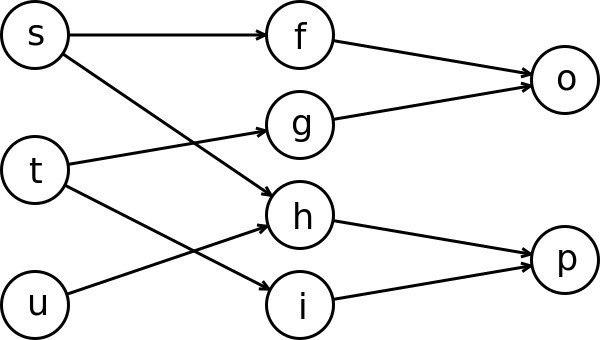
\includegraphics[scale=0.25]{scvoting_fact_coherence_counterexample}
    \caption{
        Fact-Coherence counterexample for \scvoting{}
    }
    \label{td_fig_scvoting_fact_coherence_counterexample}
\end{figure}

Consider the network shown in
\cref{td_fig_scvoting_fact_coherence_counterexample}. We have $f \feq g \feq i
\flt h$. Source-Coherence between $s$ and $t$ gives $t \slt s$. If
Fact-Coherence held we would then get $g \flt f$, but this is not the case.

\paragraph{Source-PCI.}

\begin{figure}
    \centering
    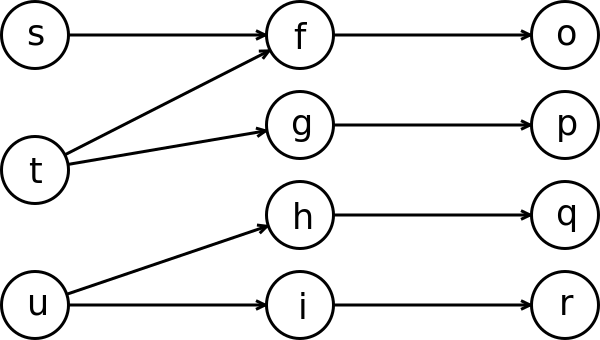
\includegraphics[scale=0.25]{scvoting_independence_counterexample}
    \caption{
        Source-PCI counterexample for \scvoting{}
    }
    \label{td_fig_scvoting_independence_counterexample}
\end{figure}

Let $N_1$ denote the top connected component of the network shown in
\cref{td_fig_scvoting_independence_counterexample}, and let $N_2$ denote the
network as a whole. The fact ranking is the same in both networks: $g \feq h
\feq i \flt f$.  In $N_1$ sources $s$ and $t$ claim a different number of
facts, so neither $s \scoh_{N_1} t$ nor $t \scoh_{N_1} s$. Consequently
$W_{N_1}(s) = W_{N_1}(t) = \emptyset$ and $s \seq_{N_1}^{T^{SCV}} t$.

In $N_2$ sources $t$ and $u$ can be compared for Source-Coherence, and we see
that $u \scoh_{N_2} t$ since $i \fle_{N_2}^{T^{SCV}} g$ and $h
\flt_{N_2}^{T^{SCV}} f$. Hence $W_{N_2}(t) = \{u\}$ and $W_{N_2}(s) =
\emptyset$, which means $s \slt_{N_2}^{T^{SCV}} t$. This contradicts
Source-PCI, which requires the ranking of $s$ and $t$ to be the same in both
networks.  \end{proof}

Note that the idea behind \scvoting{} can be generalised
beyond \voting{}: it is possible to define $\scoh_N$ in terms of \emph{any}
operator $T$, and to construct a new operator $T'$ whose source ranking is
given according to $\scoh_N$ as above, and whose fact ranking coincides with
that of $T$. This ensures $T'$ satisfies Source-Coherence whilst keeping the
existing fact ranking from $T$.

Moreover we can go in the other direction and ensure \emph{Fact}-Coherence
whilst retaining the source ranking of $T$ by defining a relation $\fcoh_N$ on
$\F$ in a analogous manner to $\scoh_N$, and proceeding similarly.

\subsubsection{Sums}

Our main concern with \sums{} is the failure of PCI and Monotonicity.  We have
seen that this is in some sense caused by the normalisation step: in
\cref{td_fig_sums_indep_poi_counterexample} the scores of $f, g$ etc go to 0 in
the limit after dividing the `global' maximum score across the network, which
happens to come from a different connected component.

A natural fix for PCI is to therefore divide by the maximum score
\emph{within each component}. In this case the score for a source $s$ depends
only on the structure of the connected component in which it lies, which is
exactly what is required for PCI.

However, this approach does not negate the undesirable effects of
\cref{td_prop_obliteration}. Indeed, suppose the network in
\cref{td_fig_sums_indep_poi_counterexample} was modified so that fact $y_1$ is
associated with object $o$ instead of $p_1$. Clearly \cref{td_prop_obliteration}
still applies after this change, and all sources and facts shown now belong to
the same connected component. Therefore the `per-component \sums{}' operator
gives the same result as \sums{} itself, and in particular our Monotonicity
counterexample still applies. Perhaps even worse, one can show that Coherence
fails for this operator. We consider the loss of Coherence too high a price to
pay for PCI.

Instead, let us take a step back and consider if normalisation is truly
necessary. On the one hand, without normalisation the trust and belief scores
are unbounded and therefore do not converge. On the other, we are not
interested in the numeric scores for their own sake, but rather for the
\emph{rankings} that they induce. It may be possible that whilst the scores
diverge without normalisation, the induced rankings \emph{do} converge to a
fixed one, which we may take as the `ordinal limit'. This is in fact the case.
We call this new operator \usums{}.

\begin{definition}

\usums{} is the recursive operator $\rec(T^{\text{prior}}, U^{\text{Sums}})$
where $T_N^{\text{prior}}(s) = 1$, $T_N^{\text{prior}}(f) = |\src_N(f)|$ and
$U^{\text{Sums}}$ is defined as in \cref{td_sec_sums_example}.\footnotemark{}

\end{definition}

\footnotetext{
    Note that to simplify proof of ordinal convergence we use a different prior
    operator to \sums{}, but this does not effect the operator in any
    significant way.
}



\begin{theorem}
\label{td_thm_usums_ordinal_convergence}
\usums{} is ordinally convergent in the following sense: there is an ordinal
operator $T^*$ such that for each network $N$ there exists $J_N \in \Nat$ such
that $T_N^n(s_1) \le T_N^n(s_2)$ iff $s_1 \sle_N^{T^*} s_2$ for all $n \ge J_N$
and $s_1, s_2 \in \S$ (and similarly for facts).

That is, the rankings induced by $T^n$ remain constant after $J_N$ iterations,
and are identical to those of $T^*$.
\end{theorem}

\begin{proof}
    The proof will use some results from linear algebra, so we will work with a
    matrix and vector representation of \usums{}. Fix an enumeration $\S =
    \{s_1,\ldots,s_k\}$ of $\S$ and $\F = \{f_1,\ldots,f_l\}$ of $\F$. Write
    $M$ for the $k \times l$ matrix given by
    \[
        [M]_{ij} = \begin{cases}
            1 & \text{ if } s_i \in \src_N(f_j) \\
            0 & \text{ otherwise }
        \end{cases}
        \quad
        (1 \le i \le k, 1 \le j \le l)
    \]
    We also write $v_n$ and $w_n$ for the vectors of trust and belief scores of
    \usums{} at iteration $n$; that is
    \[
        v_n = [T_N^n(s_1), \ldots, T_N^n(s_k)]^\top \in \R^k
    \]
    \[
        w_n = [T_N^n(f_1), \ldots, T_N^n(f_l)]^\top \in \R^l
    \]
    where $(T^n)_{n \in \Nat}$ denotes \usums{}.

    Multiplication by $M$ encodes the update step of \usums{}: it is easily
    shown that $v_{n+1} = Mw_n$ and $w_{n+1} = M^{\top}v_{n+1}$.  Writing $A =
    MM^\top \in \R^{k \times k}$, we have $v_{n+1} = Av_n$, and therefore
    $v_{n+1} = A^n v_1$.

    To show that the rankings of \usums{} remain constant after finitely many
    iterations, we will show that for each $s_p, s_q \in \S$ there is $J_{pq}
    \in \Nat$ such that $\sign([v_n]_p - [v_n]_q)$ is constant for all $n \ge
    J_{pq}$. Since $[v_n]_p$ and $[v_n]_q$ are the trust scores of $s_p$ and
    $s_q$ respectively in the $n$-th iteration, this will show that the ranking
    of $s_p$ and $s_q$ remains the same after $J_{pq}$ iterations. Since there
    are only finitely many pairs of sources, we may then take $J_N$ as the
    maximum value of $J_{pq}$ over all pairs $(p, q)$, and the entire source
    ranking ${\sle_N^{T^n}}$ of \usums{} remains constant for $n \ge J_N$. An
    almost identical argument can be carried out for the fact ranking, and
    these together will prove the result.

    So, fix $s_p, s_q \in \S$. Write $\delta_n = [v_n]_p - [v_n]_q$. First note
    that $A = MM^\top$ is symmetric, so the \emph{spectral theorem} gives the
    existence of $k$ orthogonal eigenvectors $x_1, \ldots, x_k$ for
    $A$~\cite[Theorem 7.29]{axler2014}. Let $\lambda_1, \ldots, \lambda_k$ be
    the corresponding eigenvalues. Form a $(k \times k)$-matrix $P$ whose
    $i$-th column is $x_i$, and let $D =
    \text{diag}(\lambda_1,\ldots,\lambda_k)$. Then $A$ can be diagonalised as
    $A = PDP^{-1}$. It follows that for any $n \in \Nat$, $A^n = PD^nP^{-1}$.

    Now, since $x_1,\ldots,x_k$ are orthogonal, $P$ is an orthogonal matrix, i.e.
    $P^\top = P^{-1}$. Hence $A^n = PD^nP^\top$. Note that
    \[
        PD^n
        = \begin{bmatrix}
            x_1 \mid \ldots \mid x_k
        \end{bmatrix}
        \begin{bmatrix}
            \lambda_1^n &        &             \\
                        & \ddots &             \\
                        &        & \lambda_k^n \\
        \end{bmatrix}
        = \begin{bmatrix}
            \lambda_1^n x_1 \mid \ldots \mid \lambda_k^n x_k
        \end{bmatrix}
    \]
    and
    \[
        P^{\top}v_1
        = \begin{bmatrix}
            x_1 \\ - \\ \vdots \\ - \\ x_k
        \end{bmatrix} v_1
        = \begin{bmatrix}
            x_1 \cdot v_1 \\ \vdots \\ x_k \cdot v_1
        \end{bmatrix}
    \]
    which means
    \[
        v_{n+1}
        = A^nv_1
        = PD^nP^{\top}v_1
        = \begin{bmatrix}
            \lambda_1^n x_1 \mid \ldots \mid \lambda_k^n x_k
        \end{bmatrix}
        \begin{bmatrix}
            x_1 \cdot v_1 \\ \vdots \\ x_k \cdot v_1
        \end{bmatrix}
        = \sum_{i=1}^{k}{(x_i \cdot v_1) \lambda_i^n x_i}
    \]
    We obtain an explicit formula for $\delta_{n+1}$:
    \begin{equation}
        \label{td_eqn_delta_formula}
        \delta_{n+1}
        = [v_n]_p - [v_n]_q
        = \sum_{i=1}^{k}{
            (x_i \cdot v_1) \lambda_i^n \left( [x_i]_p - [x_i]_q \right)
        }
        = \sum_{i=1}^{k}{r_i \lambda_i^n}
    \end{equation}
    where $r_i = (x_i \cdot v_1)\left( [x_i]_p - [x_i]_q \right)$. Note that
    $r_i$ does not depend on $n$.

    Now, it is easy to see that $A = MM^\top$ is \emph{positive semi-definite},
    which means its eigenvalues $\lambda_1,\ldots,\lambda_k$ are all
    non-negative. We re-index the sum in \cref{td_eqn_delta_formula} by grouping
    together the $\lambda_i$ which are equal, to get
    \[
        \delta_{n+1} = \sum_{t=1}^{K}{R_t \mu_t^n}
    \]
    where $K \le k$, each $R_t$ is a sum of the $r_i$ (whose corresponding
    $\lambda_i$ are equal), and the $\mu_t$ are distinct and non-negative.
    Assume without loss of generality that $\mu_1 > \mu_2 > \cdots > \mu_K \ge
    0$. If $R_t = 0$ for all $t$, then clearly $\sign(\delta_{n+1}) = \sign(0)
    = 0$ which is constant, so we are done. Otherwise, let $T$ be the minimal
    $t$ such that $R_t \ne 0$. We may also assume $\mu_T > 0$ (otherwise we
    necessarily have $\mu_T = 0$, $T=K$ and $\sign(\delta_{n+1}) = \sign(R_T
    \cdot 0^n)$ which is again constant 0). Observe that
    \[
        \delta_{n+1}
        = R_T \mu_T^n + \sum_{t=T + 1}^{K}{R_t \mu_t^n} \\
        = \mu_T^n \left[
            R_T + \sum_{t=T + 1}^{K}{
                R_t \left(\frac{\mu_t}{\mu_T}\right)^n
            }
        \right]
    \]
    By our assumption on the ordering of the $\mu_t$, we have $\mu_t < \mu_T$
    in the sum. Consequently $|\mu_t / \mu_T| < 1$, and $(\mu_t / \mu_T)^n \to
    0$ as $n \to \infty$. This means
    \[
        \limn{\left[
            R_T + \sum_{t=T + 1}^{K}{
                R_t \underbrace{\left(\frac{\mu_t}{\mu_T}\right)^n}_{\to 0}
            }
        \right]}
        = R_T
        \ne 0
    \]
    Since this limit is non-zero, there is $J_{pq} \in \Nat$ such that the sign
    of term in square brackets is
    equal to $S = \sign R_T \in \{1, -1\}$ for all $n \ge J_{pq}$. Finally,
    for such $n$ we have
    \[
        \sign \delta_{n+1}
        = \sign \left(
            \underbrace{\mu_T^n}_{> 0}
            \left[
                R_T + \sum_{t=T + 1}^{K}{
                    R_t \left(\frac{\mu_t}{\mu_T}\right)^n
                }
            \right]
        \right)
        = \sign \left(
            R_T + \sum_{t=T + 1}^{K}{
                R_t \left(\frac{\mu_t}{\mu_T}\right)^n
            }
        \right)
        = S
    \]
    i.e. $\sign \delta_n$ is constant for $n \ge J_{pq} + 1$. This completes
    the proof.\footnote{
        The argument which shows that the difference between fact belief scores
        is also eventually constant in sign is almost identical. Write $B =
        M^{\top}M$, and observe that $w_{n+1} = B^nw_1$. Since $B$ is also
        symmetric and positive semi-definite, the proof goes through as above.
    }
\end{proof}

In light of \cref{td_thm_usums_ordinal_convergence}, we may consider \usums{}
itself as an ordinal operator $T^*$, where $s \sle_N^{T^*} t$ iff $s
\sle_N^{T^{J_n}} t$ for each network $N$ (and similarly for the fact ranking).
Moreover, with the normalisation problems aside, \usums{} provides an example
of a principled operator satisfying our two key axioms -- Coherence and PCI. In
particular, we escape the undesirable behaviour of \sums{} in
\cref{td_fig_sums_indep_poi_counterexample}; whereas \sums{} trivialises the
ranking of sources and facts in the upper connected component, \usums{} allows
meaningful ranking (e.g. we have $g \flt f$). In particular, the counterexample
for Monotonicity for \sums{} is no longer a counterexample for \usums{}. We
conjecture that \usums{} also satisfies Monotonicity, but this remains to be
proven. For example, we have experimentally verified that \usums{} satisfies
all the specific instances of Monotonicity with the starting network $N$ as in
\cref{td_fig_intro_example}.

\begin{theorem}
\label{td_thm_usums_axioms}
\usums{} satisfies Coherence, Symmetry, Unanimity, Groundedness and
PCI. \usums{} does not satisfy POI and Strong Independence.
\end{theorem}

\begin{proof}[Proof (sketch)]
% \begin{proof}[Proof (sketch)]

The proof that \usums{} satisfies Symmetry, PCI, Unanimity and Groundedness is
routine, and we leave the details to the appendix. In what follows, let
$(T^n)_{n \in \Nat}$ denote \usums{}, $T^*$ denote the ordinal limit of
\usums{}, and for a network $N$ let $J_N$ be as in
\cref{td_thm_usums_ordinal_convergence}. Then the rankings in $N$ induced by $T^n$
for $n \ge J_N$ are the same as $T^*$.

\paragraph{Coherence.}
First we show Source-Coherence. Let $N$ be a network and suppose
$\facts_N(s_1)$ is less believable than $\facts_N(s_2)$ with respect to $N$ and
$T^*$. Let $\phi$ and $\hat{f}$ be as in the definition of less believable.

Let $n \ge J_N$. Then $f \fle_N^{T^*} \phi(f)$ and $\hat{f} \flt_N^{T^*}
\phi(\hat{f})$ for each $f \in \facts_N(s_1)$ means $T_N^n(f) \le
T_N^n(\phi(f))$ and $T_N^n(\hat{f}) < T_N^n(\phi(\hat{f}))$. Hence
\begin{align*}
    T_N^{n+1}(s)
    &= \sum_{f \in \facts_N(s_1)}{T_N^n(f)} \\
    &= T_N^n(\hat{f}) + \sum_{f \in \facts_N(s_1) \setminus \{\hat{f}\}}{T_N^n(f)} \\
    &< T_N^n(\phi(\hat{f})) + \sum_{f \in \facts_N(s_1) \setminus \{\hat{f}\}}{T_N^n(\phi(f))} \\
    &= \sum_{f \in \facts_N(s_1)}{T_N^n(\phi(f))} \\
    &= \sum_{g \in \facts_N(s_2)}{T_N^n(g)} \\
    &= T_N^{n+1}(s_2)
\end{align*}
i.e. $T_N^{n+1}(s_1) < T_N^{n+1}(s_2)$. But $T_N^{n+1}$ gives the same ranking
as $T_N^n$ and therefore the same ranking as $T^*$, so we get $s_1 \slt_N^{T^*}
s_2$ as required.

For Fact-Coherence, suppose $\src_N(f_1)$ is less trustworthy than
$\src_N(f_2)$ with respect to $N$ and $T^*$. Again, let $n \ge J_N$ and $\phi$,
$\hat{s}$ be as in the definition of less trustworthy. Recall that belief
scores for facts in $T_N^n$ are obtained from trust scores in $T_N^n$; applying
the same argument as above we get $T_N^n(f_1) < T_N^n(f_2)$ and consequently
$f_1 \fle_N^{T^*} f_2$ as required. Hence $T^*$ satisfies Coherence.

\paragraph{POI and Strong Independence.}

\begin{figure}[ht]
\centering
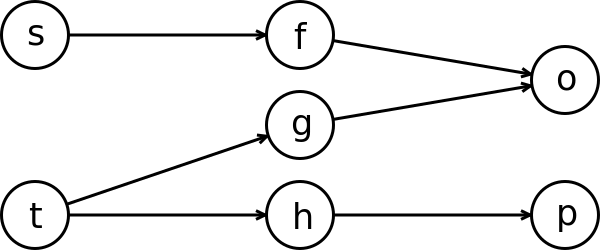
\includegraphics[scale=0.25]{usums_poi_counterexample}
\caption{
    Counterexample for POI and Strong Independence for \usums{}
}
\label{td_fig_usums_poi_counterexample}
\end{figure}

To show POI and Strong Independence are not satisfied, consider the network $N$
shown in \cref{td_fig_usums_poi_counterexample}. It can be seen (e.g. by
induction) that
\[
    T_N^n(f) = 1,
    \quad
    T_N^n(g) = 2^{n-1}
\]
for all $n \in \Nat$. Consequently $f \flt_N^{T^*} g$.\footnotemark

\footnotetext{
    Note that $g$ ranks higher than $f$ in this network simply because $t$
    makes more claims than $s$, and each fact is claimed only by a single
    source. This questionable property of \usums{} is inherited from \sums{}.
}

Now let $N'$ be the network in which the claim $(t, h)$ is removed. Since
$\src_N(f) = \src_{N'}(f) = \{s\}$ and $\src_N(g) = \src_{N'}(g) = \{t\}$, both
POI and Strong Independence imply $f \fle_N^{T^*} g$ iff $f \fle_{N'}^{T^*} g$.
Therefore assuming either of POI or Strong Independence we get $f
\flt_{N'}^{T^*} g$. However is is also clear that
\[
    T_{N'}^n(f) = T_{N'}^n(g) = 1
\]
for all $n \in \Nat$, so $f \feq_{N'}^{T^*} g$. This is a contradiction, so
neither POI nor Strong Independence are satisfied.
\end{proof}

To summarise this section, \cref{td_table_axioms} shows which axioms are
satisfied by each of the operators.

\begin{table}
\newcommand{\yes}{\checkmark}
\newcommand{\no}{\sffamily{X}}
\newcommand{\notsure}{?}
\centering
    \caption{Satisfaction of the axioms for the various operators. Recall that
    POI and Strong Independence are undesirable properties.}
    \begin{tabular}{c c c c c}
        \toprule
                         & Voting & SC-Voting  & Sums & U-Sums   \\
        \midrule
        Source-Coherence & \no    & \yes       & \yes & \yes     \\
        Fact-Coherence   & \yes   & \no        & \yes & \yes     \\
        Symmetry         & \yes   & \yes       & \yes & \yes     \\
        Unanimity        & \yes   & \yes       & \yes & \yes     \\
        Ground.          & \yes   & \yes       & \yes & \yes     \\
        Mon.             & \yes   & \yes       & \no  & \notsure \\
        Source-PCI       & \yes   & \no        & \no  & \yes     \\
        Fact-PCI         & \yes   & \yes       & \no  & \yes     \\
        \hline
        POI              & \yes   & \yes       & \no  & \no      \\
        Str. Indep.      & \yes   & \yes       & \no  & \no      \\
        \bottomrule
    \end{tabular}
\label{td_table_axioms}
\end{table}

\section{Variable domain truth discovery}
\label{td_sec_variable_domain}

So far, we have considered an arbitrary but fixed (finite) domain of sources,
facts and objects $(\S, \F, \O)$. Our operators and axioms were defined with
respect to this domain. However, the operators do not \emph{depend} on the
domain: they can be defined for \emph{any} choice of $\S$, $\F$ and $\O$. In
this section we generalise the framework so that these sets are no longer
fixed. This allows new situations to be modelled, such as new sources entering
the network. Adapting the definition of a TD operator to this case, we can then
see how the ranking of facts changes as new sources are added. Such variable
domain operators are then analogues of \emph{variable electorate voting rules}
in social theory.

Formally, let $\uS$, $\uF$ and $\uO$ be countably infinite sets of sources,
facts and objects respectively. A \emph{domain} is a triple $\D = (\S, \F,
\O)$, where $\S \subseteq \uS$, $\F \subseteq \uF$ and $\O \subseteq \uO$ are
finite, non-empty sets. We think of $\uS$, $\uF$ and $\uO$ as being the
`universe' of possible sources, facts and objects, and a domain as the (finite)
sets of entities under consideration in a particular TD problem. Given a domain
$\D = (\S, \F, \O)$, we define $\D$-networks and $\D$-operators as in
\cref{def_td_network,td_def_truth_discovery_operator}.

\begin{definition}
    A \emph{variable domain operator} $T$ is a mapping which maps each domain
    $\D$ to a $\D$-operator $T_\D$.
\end{definition}

Note that for a domain $\D = (\S, \F, \O)$ and a $\D$-network $N$,
$\sle_N^{T_\D}$ and $\fle_N^{T_\D}$ are rankings only over the set of sources
$\S$ and $\F$ in the domain $\D$, \emph{not} all of $\uS$ and $\uF$. If $\D$ is
clear from context, we write $\sle_N^T$ and $\fle_N^T$ without explicit
reference to the domain.

Since all the axioms so far were stated with respect to a fixed but arbitrary
domain, they can be easily lifted to the variable domain case. For instance, we
say a variable domain operator $T$ satisfies Coherence if $T_\D$ satisfies the
instance of Coherence for domain $\D$, for all $\D$, and similar for the other
axioms.

But we can now go further, and introduce axioms which make use of
\emph{several} domains. First, we generalise Symmetry to act across domains.
Say networks $N, N'$ in domains $\D, \D'$ respectively are \emph{equivalent} if
there is a graph isomorphism $\pi$ between them such that $\pi(s) \in \S'$,
$\pi(f) \in \F'$ and $\pi(o) \in \O'$ for all $s \in \S$, $f \in \F$ and $o \in
\O$.

\begin{axiom}[Isomorphism]
    Let $N$ and $N' = \pi(N)$ be equivalent networks. Then for all $s_1, s_2
    \in \S$, $f_1, f_2 \in \F$, we have $s_1 \sle_N^T s_2$ iff $\pi(s_1)
    \sle_{N'}^T \pi(s_2)$ and $f_1 \fle_N^T f_2$ iff $\pi(f_1) \fle_{N'}^T
    \pi(f_2)$.
\end{axiom}

Like Symmetry, Isomorphism simply says that operators only care about the
\emph{structure} of the network, not the particular `names' chosen for sources,
facts and objects. Symmetry is obtained as the special case where $N$ and $N'$
are equivalent when seen as networks in a common domain $\D$. All the operators
of \cref{td_sec_specific_operators,td_sec_modifying_voting_and_sums} satisfy
Isomorphism.

Next we introduce a new monotonicity property. In what follows, for a network
$N = (V, E)$ in domain $(\S, \F, \O)$, $f \in \F$ and $\S' \subseteq \uS$
finite and disjoint from $\S$, write $N + (\S', f)$ for the network in domain
$(\S \cup \S', \F, \O)$ with edge set $E \cup \{(s, f) \mid s \in \S'\}$, i.e.
the extension of $N$ where a collection of `fresh' sources $\S'$ each claim
$f$. For example, \cref{td_fig_eventual_mon_example} shows $N + (\S', h)$ for the
network $N$ from \cref{td_fig_intro_example} and new sources $\S' = \{x_1, \ldots,
x_4\}$.

\begin{figure}[b]
\centering
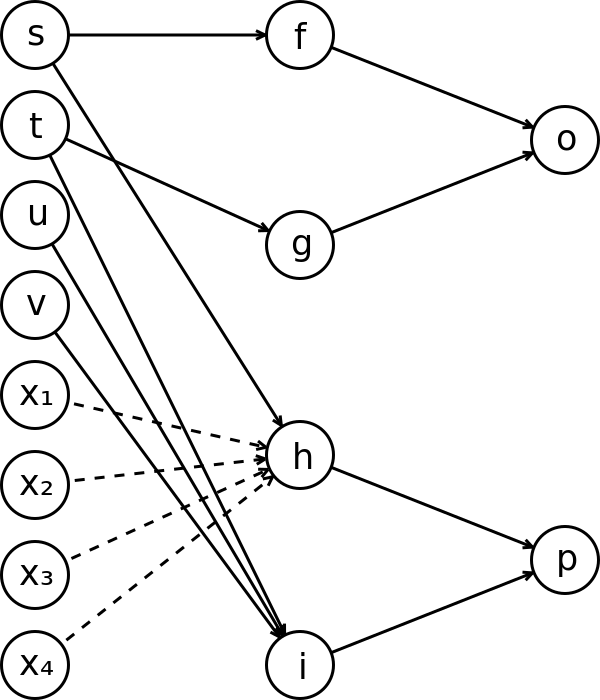
\includegraphics[scale=0.25]{eventual_mon_example}
\caption{
    $N + (\S', h)$, where $N$ is the network from \cref{td_fig_intro_example} and
    $\S' = \{x_1, \ldots, x_4\}$.
}
\label{td_fig_eventual_mon_example}
\end{figure}

\begin{axiom}[Eventual Monotonicity]
    Let $\D = (\S, \F, \O)$ be a domain and $N$ a $\D$-network. Then for all
    $f, g \in \F$, $f \ne g$, there is a finite, non-empty set $\S' \subseteq
    \uS$ with $\S \cap \S' = \emptyset$ and $g \flt_{N + (\S', f)}^T f$.
\end{axiom}

This axiom says that, given any pair of distinct facts $f, g$, it is possible
to add enough new claims for $f$ to make $f$ strictly more believable than $g$.
Intuitively, this is less demanding that Monotonicity, which requires that $f$
can become strictly more believable than $g$ with the addition of just
\emph{one} additional claim. Note that Eventual Monotonicity is not possible to
state in the fixed domain case (e.g. consider $N$ already containing claims
from all the available sources in $\S$).

When paired with Isomorphism, Eventual Monotonicity takes on a form similar to
postulates for \emph{Improvement} and \emph{Majority} operators in belief
merging~\cite{koniecznyP08_improvement,konieczny2002merging}: there is a
threshold $n \in \Nat$ such that $f$ becomes strictly more believable than $g$
after $n$ new claims are added for $f$. That is, the identities of the new
sources $\S'$ are irrelevant; it is just the \emph{size} of $\S'$ that matters.
We require a preliminary lemma.

\begin{lemma}
    \label{td_lemma_isomorphism_var_op}
    Suppose a variable domain operator $T$ satisfies Isomorphism. Let $\D = (\S,
    \F, \O)$ be a domain, $N$ a network in $\D$ and $f \in \F$. Then for all
    non-empty, finite sets $\S'_1, \S'_2 \subseteq \uS$ disjoint from $\S$ with
    $|\S'_1| = |\S'_2|$,
    \[
        {\fle_{N + (\S'_1, f)}^T}
        =
        {\fle_{N + (\S'_2, f)}^T}
    \]
\end{lemma}

\begin{proof}
    Write $\D_1 = (\S \cup \S'_1, \F, \O)$ and $\D_2 = (\S \cup \S'_2, \F,
    \O)$. Then $N + (\S'_i, f)$ is a network in domain $\D_i$ (for $i \in \{1,
    2\}$). Since $|\S'_1| = |\S'_2|$ by assumption, there is a bijection $\phi:
    \S'_1 \to \S'_2$. Define a mapping $\pi$ from $\D_1$ to $\D_2$ by
    \[
        \pi(s) = \begin{cases}
            s,& s \in \S \\
            \phi(s),& s \in \S'_1
        \end{cases}
        \quad (s \in \S \cup \S'_1)
    \]
    and $\pi(g) = g$, $\pi(o) = o$ for $g \in \F$ and $o \in \O$. Then it is
    easily verified that $\pi$ is an isomorphism from $N + (\S'_1, f)$ to $N +
    (\S'_2, f)$. For $g_1, g_2 \in \F$, we have $g_1 \fle_{N + (\S'_1, f)}^T
    g_2$ iff $\pi(g_1) \fle_{N + (\S'_2, f)}^T \pi(g_2)$ by Isomorphism. Since
    $\pi(g_1) = g_1$ and $\pi(g_2) = g_2$, this shows ${\fle_{N + (\S'_1,
    f)}^T} = {{\fle_{N + (\S'_2, f)}^T}}$.
\end{proof}

Note that since $\uS$ is infinite and domains are finite, for any $n \in \Nat$
and any domain $\D = (\S, \F, \O)$ there is always some $\S' \subseteq \uS$,
disjoint from $\S$, with $|\S'| = n$. For operators $T$ satisfying Isomorphism,
write $\fle_{N + (n \times f)}^T$ for $\fle_{N + (\S', f)}^T$;
\cref{td_lemma_isomorphism_var_op} guarantees this is well-defined (i.e. does not
depend on the particular choice of $\S'$). That is, $\fle_{N + (n \times f)}^T$
is the fact ranking resulting from adding $n$ new claims for $f$ from fresh
sources. We obtain an equivalent characterisation of Eventual Monotonicity,
whose proof is almost immediate given \cref{td_lemma_isomorphism_var_op}.

\begin{proposition}
    \label{td_prop_eventual_mon_iff_improvement}
    Suppose $T$ satisfies Isomorphism. Then $T$ satisfies Eventual Monotonicity
    if and only if for all domains $\D = (\S, \F, \O)$, all networks $N$ in
    $\D$ and distinct $f, g \in \F$, there is $n \in \Nat$ such that $g \flt_{N
    + (n \times f)}^T f$.
\end{proposition}

\begin{proof}
    `if': To show Eventual Monotonicity, take any $\S' \subseteq \uS \setminus
    \S$ of size $n$.

    `Only if': Given that Eventual Monotonicity holds, simply take $n = |\S'|$.
\end{proof}

We can now show that all operators studied so far -- when lifted to the
variable domain case -- satisfy Eventual Monotonicity.

\begin{theorem}
    \label{td_thm_operators_satisfy_eventual_mon}
    \voting{}, \sums{}, \scvoting{} and \usums{} satisfy Eventual Monotonicity.
\end{theorem}

\begin{proof}[Proof (sketch)]
    Let $\D = (\S, \F, \O)$ be a domain, $N$ a network in $\D$ and $f, g \in
    \F$. Given that Isomorphism holds for each operator, we sketch the proof
    via \cref{td_prop_eventual_mon_iff_improvement}.

    For \voting{} and \scvoting{}, we may simply take $n = 1 + |\src_N(g)|$.
    For \sums{} and \usums{}, take $n = 2 |\S| \cdot |\F|$. Write $N' = N +
    (\S', f)$ for some $\S' \subseteq \uS \setminus \S$ with $|\S'| = n$

    If $(T^k)_{k \in \Nat}$ denotes \sums{}, one can show by induction that
    $T^k_{N'}(f) = 1$ and $T^{k}_{N'}(h) \le \frac{1}{2}$ for any $h \ne f$ and
    $k > 1$, and thus $g \flt_{N'}^{T^\sums{}} f$.

    Similarly, letting $(T^k)_{k \in \Nat}$ denote \usums{}, one can show by
    induction that $T^{k}_{N'}(f) > T^{k}_{N'}(h)$ for $h \ne f$, and thus $g
    \flt_{N'}^{T^\usums{}} g$.
\end{proof}

To conclude this section, we show that the impossibility result of
\cref{td_thm_impossibility} holds in the variable domain case if one replaces
Monotonicity with Eventual Monotonicity and Symmetry with Isomorphism.

\begin{theorem}
\label{td_thm_var_dom_impossibility}
    There is no variable domain operator satisfying Coherence, Isomorphism,
    Eventual Monotonicity and POI.
\end{theorem}

\begin{proof}
    For contradiction, suppose $T$ is an operator satisfying the stated axioms.
    Let $N$ be the network from \cref{td_fig_intro_example}, viewed as a network
    in domain $(\{s, t, u, v\}, \{f, g, h, i\}, \{o, p\})$. Applying Eventual
    Monotonicity with $i$ and $h$, we have that there is $N'$ with $i
    \flt_{N'}^T h$, where $N' = N + (\S', h)$ for some $\S' \subseteq \uS
    \setminus \{s, t, u, v\}$. Since $N'$ only adds claims for $p$-facts, POI
    applied to object $o$ and Isomorphism give $f \feq_{N'}^T g$ (e.g. consider
    $\pi$ which simply swaps $s$ with $t$ and $f$ with $g$). From
    Source-Coherence we get $t \slt_{N'}^T s$. But $\src_{N'}(f) = \{s\}$ and
    $\src_{N'}(g) = \{t\}$, so Fact-Coherence gives $g \flt_{N'}^T f$:
    contradiction!
\end{proof}

\section{Discussion}
\label{td_sec_discussion}

In this section we discuss the axioms and their limitations.
%
First, the version of Monotonicity we consider is a strict one: a new claim for
$f$ gives $f$ a \emph{strictly} positive boost in the fact believability
ranking. This is also the case for Eventual Monotonicity in the variable domain
case, where we require that some number of new claims make $f$ strictly more
believable than any other fact $g$. As noted in \cref{td_sec_fact_ranking_axioms},
this assumes there is no \emph{collusion} between sources. Indeed, suppose
sources $s_1$, $s_2$ are in collusion. For example, $s_2$ may agree to
unconditionally back up all claims made by $s_1$. In this case a claim of $f$
from $s_1$ alone should carry just as much weight as the claim from both $s_1$
and $s_2$. However, Monotonicity requires that $f$ becomes strictly more
believable when moving to the latter case.

A natural solution is to simply relax the strictness requirement. We obtain the
following weak version of Monotonicity.

\begin{axiom}[Weak Monotonicity]
Let $N, s, f, N'$ be as in the statement of Monotonicity. Then for all $g \ne
f$, $g \fle_N^T$ implies $g \fle_{N'}^T f$.
\end{axiom}

Weak Monotonicity only says says that extra support for a fact $f$ does not
make $f$ \emph{less} believable. Clearly Monotonicity implies Weak
Monotonicity, but not vice versa. In the collusion example, an operator may
select to leave the fact ranking unchanged when a new report of $f$ from $s_2$
arrives; this is inconsistent with Monotonicity but consistent with Weak
Monotonicity. The weak analogue of Eventual Monotonicity can be defined in the
same way.

In the same spirit, one could consider versions of Coherence only using weak
comparisons. Say $\facts_N(s_1)$ is \emph{weakly less believable} than
$\facts_N(s_2)$ iff the condition in \cref{td_def_coherence_less_believable}
holds, but without the requirement that some $\hat{f} \in \facts_N(s_1)$ is
strictly less believable than its counterpart $\phi(\hat{f})$ in
$\facts_N(s_2)$, and define $\src_N(f_1)$ weakly less trustworthy than
$\src_N(f_2)$ in a similar way. The weak analogue of Coherence is as follows.

\begin{axiom}[Weak Coherence]

For any network $N$, $\facts_N(s_1)$ weakly less believable than
$\facts_N(s_2)$ implies $s_1 \sle_N^T s_2$, and $\src_N(f_1)$ weakly less
trustworthy than $\src_N(f_2)$ implies $f_1 \fle_N^T f_2$.

\end{axiom}

Note that Coherence does \emph{not} imply Weak Coherence. This is because Weak
Coherence relaxes both the consequent \emph{and the antecedent} in the
implications in the statement of the axiom. Whereas Coherence imposes no
constraint when $\facts_N(s_1)$ is only weakly less believable than
$\facts_N(s_2)$, Weak Coherence requires $s_1 \sle_N^T s_2$. Consequently, the
`weakness' of Weak Coherence refers to its use of weak comparisons between
sources and facts, not its logical strength in relation to Coherence.

A natural question now arises. Does the impossibility result of
\cref{td_thm_impossibility} still hold with these new axioms? We have an answer in
the negative: the `flat' operator, which sets all sources and facts equally
ranked in all networks, satisfies all the axioms of the would-be impossibility.

\begin{proposition}
    Define an operator $T$ by $s_1 \seq_N^T s_2$ and $f \feq_N^T f_2$ for all
    networks $N$, sources $s_1, s_2$ and facts $f_1, f_2$. Then $T$ satisfies
    Coherence, Weak Coherence, Symmetry, Weak Monotonicity and POI.
\end{proposition}

\begin{proof}
    Coherence holds vacuously since we can never have $\facts_N(s_1)$ less
    believable than $\facts_N(s_2)$ or $\src_N(f_1)$ less believable than
    $\src_N(f_2)$. Since \emph{any} weak ranking holds for $T$, the other
    axioms are straightforward to see.
\end{proof}

This shows that (strict) Monotonicity is required for the impossibility result,
since the result is no longer true when relaxing to Weak Monotonicity.

We now consider the new axioms in relation to the operators. First, Weak
Coherence.

\begin{proposition}
    \label{td_prop_weak_coherence_satisfaction}
    \voting{}, \sums{} and \usums{} satisfy Weak Coherence
\end{proposition}

\begin{proof}[Proof (sketch)]\leavevmode

    \paragraph{\voting{}.} Since $s_1 \sle_N^{T^\voting{}} s_2$ always holds,
    Weak Source-Coherence clearly holds. For Weak Fact-Coherence, suppose
    $\src_N(f_1)$ is weakly less trustworthy than $\src_N(f_2)$. Then there is
    a bijection $\phi: \src_N(f_1) \to \src_N(f_2)$, so $|\src_N(f_1)| =
    |\src_N(f_2)|$. By definition of \voting{}, $f_1 \feq_N^{T^\voting{}} f_2$.
    In particular, $f_1 \flt_N^{T^\voting{}} f_2$.

    \paragraph{\sums{}.} First, one may adapt \cref{td_def_num_less_believable} to
    a numerical variant of a set of facts $Y$ being \emph{weakly} less
    believable than $Y'$, by dropping all references to $\rho$. We then have an
    analogue of \cref{td_lemma_source_coherence_lemma}, and Weak Coherence for
    \sums{} follows by an argument similar to the one used to show Coherence
    using \cref{td_lemma_source_coherence_lemma}.

    \paragraph{\usums{}.} The proof that \usums{} satisfies Coherence can be
    adapted in a straightforward way to show Weak Coherence.
\end{proof}

\Cref{td_prop_weak_coherence_satisfaction} indicates that Weak Coherence may in
fact be too weak to capture the original intuition behind Coherence -- namely,
that there should be a mutual dependence between trustworthy sources and
believable facts -- since it does not even rule out \voting{}. Instead, Weak
Coherence can be seen as a simple requirement which only rules out undesirable
behaviour, and complements (strict) Coherence.

Since Monotonicity implies Weak Monotonicity, it is clear that \voting{}
satisfies Weak Monotonicity. We conjecture that Weak Monotonicity also holds
for \sums{} and \usums{}, but this remains to be proven.\footnote{Indeed, we
conjectured in \cref{td_sec_satisfaction_of_axioms} that the stronger axiom
(strict) Monotonicity holds for \usums{}. As with Monotonicity, experimental
evidence from various starting networks $N$ suggests that Weak Monotonicity is
likely to hold.}

\section{Related work}
\label{td_sec_relatedwork}

In this section we discuss related work.

\paragraph{Ranking systems.} Altman and Tennenholtz~\cite{altman2008} initiated
axiomatic study of ranking systems. First we discuss their framework in
relation to ours, and then turn to their axioms. In their framework, a ranking
system $F$ maps any (finite) directed graph $G = (V, E)$ to a total preorder
$\le_G^F$ on the vertex set $V$. In their view this is a variation of the
classical social choice setting, in which the set of voters and alternatives
coincide. Nodes $v \in V$ ``vote" on their peers in $V$ by a form of
approval voting~\cite{laslier2010handbook}: an edge $v \to u$ is interpret as a
vote for $u$ from $v$. A ranking system then outputs a ranking of $V$,
following the general intuition that the more ``votes" $v$ receives (i.e. the
more incoming edges), the higher $v$ should rank. As with the ranking of facts
in truth discovery, this does not necessarily mean ranking nodes simply by
the \emph{number} of votes received, since the \emph{quality} of the voters
should also be taken in account. For example, a ranking system may prioritise
nodes which receive few votes from highly ranked nodes over those with many
votes from lower ranked nodes.

Note that our truth discovery networks $N$ are themselves directed graphs on
the vertex set $\S \cup \F \cup \O$. However, naively applying a ranking system
to $N$ directly makes little sense: sources never receive any ``votes", and the
resulting ranking includes objects, which do not need to be ranked in our
setting. Perhaps a more sensible approach is to consider the bipartite graph
$G_N = (V_N, E_N)$ associated with a network $N$, where
\[
    V_N = \S \cup \F,
    \qquad
    E_N =
    \bigcup_{(s, f) \in N}{
        \{(s, f), (f, s)\}
    }.
\]
That is, we take the edges from sources to facts together with the reversal of
such edges. The edges in $G_N$ have some intuitive interpretation: a source
votes for the facts which it claims are true, and a fact votes for the sources
who vouch for it. Any ranking system $F$ thus gives rise to a truth discovery
operator, where $s_1 \sle_N^T s_2$ iff $s_1 \le_{G_N}^F s_2$, and similar for
facts.

However, some characteristic aspects of the truth discovery problem are lost in
this translation to ranking systems. Notably, the objects play no role at all
in $G_N$. Sources and facts are also treated symmetrically, where they perhaps
should not be. For example, a fact $f$ receiving more claims than $g$ is
beneficial for $f$, all else being equal (see Monotonicity), but a source $s$
claiming more facts than $t$ does not tell us anything about the relative
trustworthiness of $s$ and $t$.

While other choices of $G_N$ may be possible to alleviate some of these
problems, we believe the truth discovery is sufficiently specialised beyond
general graph ranking so that a bespoke modelling is required to capture its
nuances appropriately. Our framework provides this novel contribution.

In \cite{altman2008}, Altman and Tennenholtz also introduce axioms for ranking
systems. Their first set of axioms deal with the transitive effects of voting
when the alternatives are the voters themselves. As mentioned in
\cref{td_sec_axioms}, these axioms provided the inspiration for Coherence. The
core idea is that if the predecessors of a node $v$ are weaker than those of
$u$, then $v$ should be ranked below $u$. If $v$ additionally has \emph{more}
predecessors, $v$ should rank \emph{strictly} below. Coherence applies this
idea both in the direction of sources-to-facts (Fact-Coherence) and from
facts-to-sources (Source-Coherence). A notable difference is that we only
consider the case where the number of sources for two facts (or the number of
facts, for two sources) is the same. For example, a source claiming more facts
does not give it the strict boost Transitivity would dictate. Under the mapping $N
\mapsto G_N$ described above, any ranking system satisfying Transitivity
induces a truth discovery operator which satisfies Coherence.

The other axiom in \cite{altman2008} is an independence axiom RIIA (ranked
independence of irrelevant alternatives), which adapts the classical IIA axiom
from social choice theory to the ranking system setting, although in a
different manner to our independence axioms of \cref{td_sec_indep_axioms}. We
describe the axiom in rough terms, deferring to the paper for the technical
details. Suppose the relative ranking of $u_1$'s predecessors compared to
$u_2$'s predecessors is the same as that of $v_1$'s compared to $v_2$'s. Then
RIIA requires $u_1 \le u_2$ iff $v_1 \le v_2$. Informally, ``the relative
ranking of two agents must only depend on the pairwise comparison of the ranks
of their predecessors"~\cite{altman2008}.
%
While we do not have an analogous axiom, the idea can be adapted to truth
discovery networks. Intuitively, such an axiom would state that the ranking of
two facts depends only on comparisons between their
corresponding sources (and similar for the ranking of sources).

However, the main result of Altman and Tennenholtz is an impossibility:
Transitivity is incompatible with RIIA. Moreover, the result remains true even
when restricting to bipartite graphs, such as $G_N$ described above.
Accordingly, we can expect a similar impossibility result to hold in the truth
discovery setting between Coherence and any analogue of RIIA.

\paragraph{PageRank.} PageRank~\cite{page_pagerank_1999} is a well-known
algorithm for ranking web pages based on the hyperlink structure of the web,
viewed as a directed graph. It has also been studied through the lens of social
choice and characterised
axiomatically~\cite{altman2005ranking,skibski_pagerank}.\footnote{
    Wąs and Skibski~\cite{skibski_pagerank} axiomatise the \emph{numerical
    scores} of PageRank, whereas Altman and
    Tennenholtz~\cite{altman2005ranking} axiomatise the resulting ranking.
    Moreover, Wąs and Skibski point out that Altman and Tennenholtz in fact
    only consider a simplified version of PageRank called \emph{Katz prestige},
    defined only for strongly connected graphs.
} In ~\cite{altman2005ranking} the authors propose several \emph{invariance
axioms}, each of which requires that the ranking of pages is not affected by a
certain transformation of the web graph. For example, the axiom \emph{Self
Edge} says that adding a self loop from a page $a$ to itself does not change the relative
ranking of other pages, and results in a strictly positive boost for $a$ (c.f.
Monotonicity). However, if we identify a truth discovery network $N$ with the
graph $G_N$ as described above, most of the transformations involved do not
respect the bipartite, symmetric structure of $G_N$. That is, the transformed
graph does not correspond to any $G_{N'}$, for a network $N'$. Consequently,
the PageRank axioms have no truth discovery counterpart in our
setting. The only exception is \emph{Isomorphism}, where the transformation
in question is graph isomorphism; this axiom is analogous to our Symmetry and
Isomorphism axioms. However, since PageRank is similar to the \emph{Hubs and
Authorities}~\cite{kleinberg1999} algorithm on which Sums is based -- which
also uses the link structure of the web to rank pages -- we expect there may be
additional axioms which can be expressed both for general graphs \emph{and}
truth discovery networks, satisfied by PageRank and Sums. We leave the task of
finding such axioms to future work.

\section{Summary}
\label{td_sec_conclusion}

In this paper we formalised a mathematical framework for truth discovery. While
a number of simplifying assumptions were made compared to the mainstream truth
discovery literature, we are able to express several algorithms in the
framework. This provided the setting for the axiomatic method of social choice
to be applied. To our knowledge, this is the first such axiomatic treatment in
this context.

It was possible to adapt many axioms from social choice theory and related
areas. In particular, the \emph{Transitivity} axiom studied in the context of
ranking systems~\cite{tennenholtz2004,altman2008} took on new life in the form
of Coherence, which we consider a core axiom for TD operators.
We proceeded to establish the differences between our setting and classical
social choice by considering independence axioms. This led to an impossibility
result and an axiomatic characterisation of the baseline \voting{} method.

On the practical side, we analysed the existing TD algorithm \sums{} and found
that, surprisingly, it fails PCI. This is a serious issue for \sums{} which has
not been discussed in the literature to date, and its discovery here highlights
the benefits of the axiomatic method. To resolve this, we suggested a
modification to \sums{} -- which we call \usums{} -- for which PCI \emph{is}
satisfied. However, while \usums{} resolves axiomatic problems with \sums{}, it
may introduce computational difficulties (since the numeric scores involved
grow without bound). We leave further investigation of such issues to future
work.

A restriction of our analysis is that only one `real-world' algorithm was
considered. Further axiomatic analysis of algorithms provides a deeper
understanding of how algorithms operate on an intuitive level, but is made
difficult by the complexity of the state-of-the-art truth discovery methods.
New techniques for establishing the satisfaction (or otherwise) of axioms would
be helpful in this regard.

There is also scope for extensions to our model of truth discovery in the
framework itself. For example, even in the variable domain setting of
\cref{td_sec_variable_domain}, we make the somewhat simplistic assumption that
there are only finitely many possible facts for sources to claim. This
effectively means we can only consider \emph{categorical values}; modelling an
object whose domain is the set of real numbers, for example, is not
straightforward in our framework.

Next, our model does not account for any associations or constraints between
objects, whereas in reality the belief in a fact for one object may strengthen
or weaken our belief in other facts for related objects. These types of
constraints or correlations have been studied both on the theoretical side
(e.g. in judgment aggregation) and practical side in truth
discovery~\cite{yang_probabilistic_2019}.

The axioms can also be further refined to relax some of the simplifying
assumptions we make regarding source attitudes; e.g. that they do not collude
or attempt to manipulate. Most notably, Monotonicity should be weakened to
account for such sources.

Finally, it may be argued that truth discovery as formulated in this paper
risks simply to find \emph{consensus} among sources, rather than the
\emph{truth}. To remedy this, the framework could be extended to model the
possible states of the world and thus the \emph{ground truth}
(c.f.~\cite{meir_proxy_2019}). Upon doing so one could investigate how well,
and under what conditions, an operator is able to recover the truth from a TD
network. Such truth-tracking methods have also been studied in judgment
aggregation and belief
fusion~\cite{everaere_epistemic_2010,hartmann_judgment_2012}.

}

{
    \newcommand{\ch}{\mathcal{C}}
\newcommand{\minch}[1]{\operatorname{\mathcal{M}}\left({#1}\right)}
\newcommand{\minchmon}[1]{\operatorname{\mathcal{M}}_{\mathsf{mon}}\left({#1}\right)}
\newcommand{\minchw}[2]{\operatorname{\mathcal{M}_{#1}}({#2})}
\newcommand{\mindist}[1]{m({#1})}
\newcommand{\T}{T}
\newcommand{\K}{\mathcal{K}}
\newcommand{\N}{\mathbb{N}}
\newcommand{\R}{\mathbb{R}}
\newcommand{\ale}{\preceq}
\newcommand{\alt}{\prec}
\newcommand{\aeq}{\approx}
\newcommand{\asymb}{\mathcal{A}}
\newcommand{\bsymb}{\mathcal{B}}
\newcommand{\anle}{\leqslant^{\asymb}}
\newcommand{\aneq}{\approx^{\asymb}}
\newcommand{\anlt}{<^{\asymb}}
\newcommand{\bnle}{\leqslant^{\bsymb}}
\newcommand{\ble}{\sqsubseteq}
\newcommand{\blt}{\sqsubset}
\newcommand{\beq}{\approx}
\newcommand{\tr}{\top}
\newcommand{\dual}[1]{{\overline{#1}}}
\newcommand{\vect}{\operatorname{vec}}
\newcommand{\argmin}{\operatorname*{arg\ min}}
\newcommand{\argmax}{\operatorname*{arg\ max}}
\newcommand{\rs}{\upharpoonright}
\newcommand{\dotprod}{\bullet}
\newcommand{\tpos}[1]{\operatorname{\mathcal{L}}({#1})}
\newcommand{\expectation}[2]{\operatorname*{\mathbb{E}}_{#1}{#2}}
\newcommand{\orderings}[1]{\operatorname*{\mathcal{L}}({#1})}
\newcommand{\cherr}{\varepsilon}
\newcommand{\avgmin}{\text{avg}}
\newcommand{\symdiff}{\mathrel{\triangle}}
\newcommand{\Tcount}{{\T_{\mathsf{count}}}}
\newcommand{\Tcardint}{{\T_{\mathsf{CI}}}}
\newcommand{\Tlex}{{\T_{\mathsf{lex}}}}
\newcommand{\tuple}[1]{\langle{#1}\rangle}
\newcommand{\ranks}[1]{\mathsf{ranks}({#1})}
\renewcommand{\intop}[1]{{\T_{#1}^\mathsf{int}}}
\newcommand{\swap}[3]{\mathsf{swap}({#1}; {#2}, {#3})}

% axioms
\newcommand{\chainmin}{\axiomref{Chain-min}}
\newcommand{\anon}{\axiomref{Anon}}
\newcommand{\dualaxiom}{\axiomref{Dual}}
\newcommand{\iim}{\axiomref{IIM}}
\newcommand{\mon}{\axiomref{Mon}}
\newcommand{\posresp}{\axiomref{Pos-resp}}
\newcommand{\chaindef}{\axiomref{Chain-def}}
\newcommand{\smi}{\axiomref{SMI}}
\newcommand{\rankremoval}{\axiomref{Rank-removal}}
\newcommand{\argmaxaxiom}{\axiomref{Argmax}}

    \chapter{Bipartite Tournaments}
\label{chapter_bipartite_tournaments}

A tournament consists of a finite set of players equipped with a \emph{beating
relation} describing pairwise comparisons between each pair of players.
Determining a ranking of the players in a tournament has applications in
\emph{voting}~\cite{brandt2016a}, where players represent alternatives and $x$
beats $y$ if a majority of voters prefer $x$ over $y$, \emph{paired comparisons
analysis}~\cite{gonzalez2014paired}, where players represent products and the
beating relation expresses the preferences of a consumer, \emph{search
engines}~\cite{slutzki2006scoring}, \emph{sports}~\cite{bozoki2016application}
and other domains.

In this chapter we introduce \emph{bipartite tournaments}, which consist of two
disjoint sets of players $A$ and $B$ such that comparisons only take place
between players from opposite sets. We consider ranking methods which produce
two rankings for each tournament -- one for each side of the bipartition. Such
tournaments model situations in which two different kinds of entity compete
\emph{indirectly} via matches against entities of the opposite kind.

The notion of competition may be abstract, which allows the model to be applied
in a variety of settings. However, the principal motivation in the context of this
thesis is the ranking of information sources by \emph{expertise} or
\emph{trustworthiness}, as expressed by the following example.

\begin{example}
    \label{tourn_ex_td_example}
    Consider a truth discovery setting in which information sources $\{a_1,
    \ldots, a_m\}$ provide possible values to a number of objects. Among
    these objects, the ``ground truth'' values are known for a subset $\{b_1,
    \ldots, b_n\}$, and thus for any pair $(a, b)$ it is known whether $a$
    provided the correct value or not. A natural question arises: how can the
    sources be ranked based on their trustworthiness?

    The straightforward approach of simply counting the number of correct
    values fails when the objects vary in \emph{difficulty}. Indeed, it may be
    preferable to reward sources for correct values on difficult objects, or
    to penalise them for failing on easy objects. Furthermore, the notion of
    difficulty is not intrinsic to an object, but depends on how easily
    sources are able to determine its correct value.\footnotemark{}

    The setting of bipartite tournament ranking addresses these issues.
    Indeed, the two kinds of ``players'' are the sources and objects; a source
    ``beats'' a object by providing the correct value, and otherwise the object
    beats the source. While we wish to compare sources based on their
    trustworthiness and objects based on their difficulty, there are no direct
    source-to-source or object-to-objects comparisons available: the ranking
    must be constructed on the basis of the indirect patterns of correctness
    between the set of sources and objects.
\end{example}

\footnotetext{
    This is reminiscent of the mutual dependence between trustworthiness of
    sources and belief in claims in truth discovery.
}

Note that this is related to but not the same as the ranking problem of truth
discovery itself, as studied in \cref{chapter_td}, since it does not concern
finding the true values associated with objects. The setting of
\cref{tourn_ex_td_example} is clearly relevant for \emph{semi-supervised truth
discovery}, in which a subset of ground truth is
available~\cite{yin_supervised_2011,rekatsinas2017slimfast}. However, even when
no such ground truth is available, many recursive operators (including those
described in \cref{td_new_sec_recursive_operators}) iteratively update source
trust scores on the basis of current \emph{estimates} of the true values for
objects. One could therefore consider a bipartite tournament at each stage of
the iteration. This may lead to \emph{difficulty-aware} truth discovery methods
(c.f. \textcite{galland2010}).

\label{tourn_education_example}
A related example is education~\cite{jiao2017algorithms}, where $A$ represents
students, $B$ exam questions, and student $a$ ``beats'' question $b$ by
answering it correctly. The ranking of students then reflects their
proficiency, and the ranking of questions reflects their difficulty. This may
be particularly useful in the context of automated grading of crowdsourced
questions provided by students themselves, which may vary in their difficulty
(see for example the PeerWise system \cite{denny_peerwise_2008}).

Other application domains include the evaluation of generative models in
machine learning~\cite{olsson2018skill} (where $A$ represents generators and
$B$ discriminators) and solo sports contests (e.g. where $A$ represents golfers
and $B$ golf courses). In the remainder of the chapter we take the abstract
view in which $A$ and $B$ are simply ``players'', without any fixed
interpretation. However, we keep \cref{tourn_ex_td_example} in mind as our
motivating example.

In principle, bipartite tournaments are a special case of \emph{generalised}
tournaments
\cite{gonzalez2014paired,slutzki2005ranking,csato2019impossibility}, which
allow intensities of victories and losses beyond a binary win or loss (thus
permitting draws or multiple comparisons), and do not require that every
player is compared to all others. However, many existing ranking methods in
the literature do not apply to bipartite tournaments due to the violation of an
\emph{irreducibility} requirement, which requires that the tournament graph is
strongly connected. In any case, bipartite tournament ranking presents a unique
problem -- since we aim to rank players with only indirect information
available -- which we believe is worthy of study in its own right.

In this work we focus particularly on ranking via \emph{chain graphs} and
\emph{chain editing}. A chain graph is a bipartite graph in which the
neighbourhoods of vertices on one side form a chain with respect to set
inclusion. A (bipartite) tournament of this form represents an ``ideal''
situation in which the capabilities of the players are perfectly nested: weaker
players defeat a subset of the opponents that stronger players defeat. In this
case a natural ranking can be formed according to the set of opponents defeated
by each player. These rankings respect the tournament results in an intuitive
sense: if a player $a$ defeats $b$ and $b'$ ranks worse than $b$, then $a$ must
defeat $b'$ also.
%
Unfortunately, this perfect nesting may not hold in reality: a weak player may
win a difficult match by coincidence, and a strong player may lose a match by
accident.
%
With this in mind, \textcite{jiao2017algorithms} suggested an appealing ranking
method for bipartite tournaments: apply \emph{chain editing} to the input
tournament -- i.e. find the minimum number of edge changes required to form a
chain graph -- and output the corresponding rankings. Whilst their work
focused on algorithms for chain editing and its variants, we look to study the
properties of the ranking method itself through the lens of computational social
choice.

\paragraph{Contributions.}

Our primary contribution is the introduction of a
class of ranking mechanisms for bipartite tournaments defined by chain editing.
We also provide a new probabilistic characterisation of chain editing via
maximum likelihood estimation. To our knowledge this is the first in-depth
study of chain editing as a ranking mechanism. Secondly, we introduce a new
class of ``chain-definable'' mechanisms by relaxing the minimisation constraint
of chain editing in order to obtain tractable algorithms and to resolve the
failure of an important anonymity axiom. We present a concrete example of such
an algorithm, and characterise it axiomatically.

This chapter is an extension of \textcite{singleton_booth_bipartite}, with new
results presented in \cref{tourn_sec_axiomatic_characterisation_of_tcardint}.

\section{Preliminaries}
\label{tourn_sec_preliminaries}

In this section we define our framework for bipartite tournaments, introduce
chain graphs and discuss the link between them.

\subsection{Bipartite Tournaments}

Following the literature on generalised
tournaments~\cite{gonzalez2014paired, slutzki2005ranking,
csato2019impossibility}, we represent a tournament as a matrix, whose entries
represent the results of matches between participants. In what follows, $[n]$
denotes the set $\{1,\ldots,n\}$ whenever $n \in \N$.

\begin{definition}%[Bipartite Tournament]

    A \emph{bipartite tournament} -- hereafter simply a \emph{tournament} -- is
    a triple $(A, B, K)$, where $A = [m]$ and $B = [n]$ for some $m, n \in \N$,
    and $K$ is an $m \times n$ matrix with $K_{ab} \in \{0, 1\}$ for all $(a,
    b) \in A \times B$. The set of all tournaments will be denoted by $\K$.

\end{definition}

Here $A$ and $B$ represent the two sets of players in the
tournament.\footnotemark{} An entry $K_{ab}$ gives the result of the match
between $a \in A$ and $b \in B$: it is 1 if $a$ defeats $b$ and 0 otherwise.
Note that we do not allow for the possibility of draws, and every $a \in A$
faces every $b \in B$.
%
When there is no ambiguity we denote a tournament simply by $K$, with the
understanding that $A = [\text{rows}(K)]$ and $B = [\text{columns}(K)]$.

The \emph{neighbourhood} of a player $a \in A$ in $K$ is the set $K(a) = \{b
\in B \mid K_{ab} = 1\} \subseteq B$, i.e. the set of players which $a$
defeats. The neighbourhood of $b \in B$ is the set $K^{-1}(b) = \{a \in A \mid
K_{ab} = 1\} \subseteq A$, i.e. the set of players defeating $b$.

\footnotetext{
    Note that $A$ and $B$ are not disjoint as sets: $1$ is always contained in
    both $A$ and $B$, for instance. This poses no real problem, however, since
    we view the number $1$ merely a \emph{label} for a player. It will always
    be clear from context whether a given integer should be taken as a label
    for a player on the $A$ side or the $B$ side.
}

Given a tournament $K$, our goal is to place a ranking on each of $A$ and $B$.
We define a tournament ranking operator for this purpose.

\begin{definition}%[Operator]

    An \emph{tournament ranking operator} $\T$ assigns each tournament $K$ a
    pair $\T(K) = ({\ale_K^\T}, {\ble_K^\T})$ of total preorders on $A$ and $B$
    respectively.

\end{definition}

For $a, a' \in A$, we interpret $a \ale_K^\T a'$ to mean that $a'$ is ranked
\emph{at least as strong} as $a$ in the tournament $K$, according to the
operator $\T$ (similarly, $b \ble_K^\T b'$ means $b'$ is ranked at least as
strong as $b$). The strict and symmetric parts of ${\ale_K^\T}$ are denoted
by ${\alt_K^\T}$ and ${\aeq_K^\T}$.

As a simple example, consider $\Tcount$, where $a \ale_K^\Tcount a'$ iff
$|K(a)| \le |K(a')|$ and $b \ble_K^\Tcount b'$ iff $|K^{-1}(b)| \ge
|K^{-1}(b')|$. This operator simply ranks players by number of victories. It is
a bipartite version of the \emph{points system} introduced
by~\textcite{rubinstein1980ranking}, and generalises \emph{Copeland's
rule}~\cite{brandt2016a}.

\subsection{Chain Graphs}

Each bipartite tournament $K$ naturally corresponds to a bipartite graph $G_K$,
with vertices $A \sqcup B$ and an edge between $a$ and $b$ whenever $K_{ab} =
1$.\footnotemark{} The task of ranking a tournament admits a particularly
simple solution if this graph happens to be a \emph{chain graph}.

\footnotetext{
    $A \sqcup B$ is the \emph{disjoint union} of $A$ and $B$, which we define
    as $\{(a, 0) \mid a \in A\} \cup \{(b, 1) \mid b \in B\}$.
}

%\begin{definition}[Chain graph~\cite{yannakakis1981computing}]
\begin{definition}[\textcite{yannakakis1981computing}]
\label{tourn_def_chain_graph}

    A bipartite graph $G = (U, V, E)$ is a \emph{chain graph} if there is an
    ordering $U = \{u_1,\ldots,u_k\}$ of $U$ such that $N(u_1) \subseteq \cdots
    \subseteq N(u_k)$, where $N(u_i) = \{v \in V \mid (u_i, v) \in E\}$ is the
    neighbourhood of $u_i$ in $G$.

\end{definition}

\begin{figure}
    \centering
    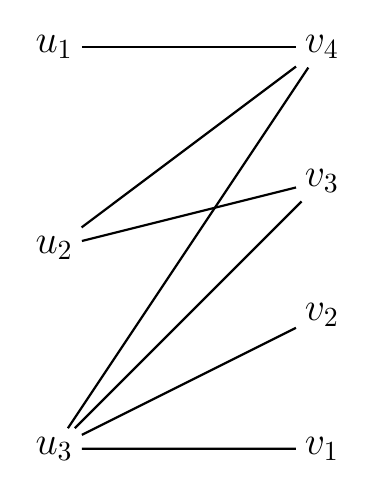
\begin{tikzpicture}[thick,scale=1.7]

        \def \m {3}
        \def \n {4}
        \def \width {2}
        \def \height {3}

        \footnotesize

        % Draw vertices
        \foreach \a in {1,...,\m} {
            \def \y {\height * (\a - 1) / (\m - 1)}
            \node (a-\a) at (0, -{\y}) {\Large $u_{\a}$};
        }
        \foreach \b in {1,...,\n} {
            \def \y {\height * (\b - 1) / (\n - 1)}
            \def \index {\pgfmathparse{int(1 + \n - \b)}\pgfmathresult}
            \node (b-\b) at (\width, -{\y}) {\Large $v_{\index}$};
        }
        % Draw edges
        \def \drawedge#1#2{\draw[-] (a-#1) -- (b-#2);}
        \drawedge{1}{1}
        \drawedge{2}{1} \drawedge{2}{2}
        \drawedge{3}{1} \drawedge{3}{2} \drawedge{3}{3} \drawedge{3}{4}

    \end{tikzpicture}
    \caption{An example of a chain graph}
    \label{tourn_fig_chain_graph_example}
\end{figure}

In other words, a chain graph is a bipartite graph where the neighbourhoods of
the vertices on one side can be ordered so as to form a chain with respect to
set inclusion. It is easily seen that this nesting property holds for $U$ if
and only if it holds for $V$. \Cref{tourn_fig_chain_graph_example} shows an example
of a chain graph.

Now, as our terminology might suggest, the neighbourhood $K(a)$ of some player
$a \in A$ in a tournament $K$ coincides with the neighbourhood of the
corresponding vertex in $G_K$. If $G_K$ is a chain graph we can therefore
enumerate $A$ as $\{a_1,\ldots,a_m\}$ such that $K(a_i) \subseteq K(a_{i+1})$
for each $1 \le i < m$. This indicates that each $a_{i+1}$ has performed
\emph{at least as well} as $a_i$ in a strong sense: every opponent which $a_i$
defeated was also defeated by $a_{i+1}$, and $a_{i+1}$ may have additionally
defeated opponents which $a_i$ did not.\footnotemark{} It seems only natural in
this case that one should rank $a_i$ (weakly) below $a_{i+1}$.
%
\footnotetext{
    Note that this is a more robust notion of performance than comparing the
    neighbourhoods of $a_i$ and $a_{i+1}$ by \emph{cardinality}, which may fail
    to account for differences in the strength of opponents when counting wins
    and losses.
}
%
Appealing to transitivity and the fact that each $a \in A$ appears as
\emph{some} $a_i$, we see that any tournament $K$ where $G_K$ is a chain graph
comes pre-equipped with a natural total preorder on $A$, where $a'$ ranks
higher than than $a$ if and only if $K(a) \subseteq K(a')$. The duality of the
neighbourhood-nesting property for chain graphs implies that $B$ can also be
totally preordered, with $b'$ ranked higher than $b$ if and only if $K^{-1}(b)
\supseteq K^{-1}(b')$.\footnotemark{}
%
Moreover, these total preorders relate to the tournament results in an
important sense: if $a$ defeats $b$ and $b'$ ranks worse than $b$, then $a$
must defeat $b'$ also. That is, the neighbourhood of each $a \in A$ is
\emph{downwards closed} w.r.t the ranking of $B$, and the neighbourhood of each
$b \in B$ is \emph{upwards closed} in $A$.

\footnotetext{
    Note that the ordering of the $B$s is reversed compared to the $A$s, since
    the larger $K^{-1}(b)$ the \emph{worse} $b$ has performed.
}

Tournaments corresponding to chain graphs will be said to satisfy the
\emph{chain property}, and will accordingly be called \emph{chain tournaments}.
We give a simpler (but equivalent) definition which does not refer to the
underlying graph $G_K$. First, define relations ${\anle_K}, {\bnle_K}$ on
$A$ and $B$ respectively by $a \anle_K a'$ iff $K(a) \subseteq K(a')$ and $b
\bnle_K b'$ iff $K^{-1}(b) \supseteq K^{-1}(b')$, for any tournament $K$.

\begin{definition}%[Chain property]
    A tournament $K$ has the \emph{chain property} if $\anle_K$ is a total
    preorder.
\end{definition}

According to the duality principle mentioned already, the chain property
implies that $\bnle_K$ is also a total preorder. Note that the relations
$\anle_K$ and $\bnle_K$ are analogues of the \emph{covering relation} for
non-bipartite tournaments \cite{brandt2016a}.

\begin{example}
    Consider
    $
        K = \left[\begin{smallmatrix}
            1 & 0 & 0 & 0 \\
            1 & 1 & 0 & 0 \\
            1 & 1 & 1 & 1
        \end{smallmatrix}\right]
    $. Then $K(1) \subset K(2) \subset K(3)$, so $K$ has the chain
    property.  In fact, $K$ is the tournament corresponding to the chain graph
    $G$ from \Cref{tourn_fig_chain_graph_example}.

\end{example}

\section{Ranking via Chain Editing}
\label{tourn_sec_ranking_via_chain_editing}

We have seen that chain tournaments
come equipped with natural rankings of $A$ and $B$. Such tournaments represent
an ``ideal'' situation, wherein the abilities of the players on both sides of the
tournament are perfectly nested. Of course this may not be so in reality:
the nesting may be broken by some $a \in A$ winning a match it ought not to by
chance, or by losing a match by accident.

One idea for recovering a ranking in this case, originally suggested
by \textcite{jiao2017algorithms}, is to apply \emph{chain editing}: find the
minimum number of edge changes required to convert the graph $G_K$ into a chain
graph. This process can be seen as correcting the ``noise'' in an observed
tournament $K$ to obtain an ideal ranking. In this section we introduce the
class of operators producing rankings in this way.

\subsection{Chain-minimal Operators}

To define chain-editing in our framework we once again present an equivalent
definition which does not refer to the underlying graph $G_K$: the number of
edge changes between graphs can be replaced by the \emph{Hamming distance}
between tournament matrices.

\begin{definition}
    For $m, n \in \N$, let $\ch_{m,n}$ denote the set of all $m \times n$
    chain tournaments. For an $m \times n$ tournament $K$,
    write $\minch{K} = \argmin_{K' \in \ch_{m,n}}{d(K, K')} \subseteq \K$ for
    the set of chain tournaments closest to $K$ w.r.t the Hamming
    distance $d(K, K') = |\{(a,b) \in A \times B \mid K_{ab} \ne K'_{ab}\}|$.
    Let $\mindist{K}$ denote this minimum distance.
\end{definition}

Note that chain editing, which is \complexityclass{NP}-hard in
general~\cite{jiao2017algorithms}, amounts to finding a single element of
$\minch{K}$.\footnotemark{} We comment further on the computational complexity
of chain editing in \Cref{tourn_sec_related_work}. The following
property characterises chain editing-based operators $\T$.

\footnotetext{
    The decision problem associated with chain editing -- which in tournament
    terms is the question of whether $\mindist{K} \le k$ for a given integer
    $k$ -- is \complexityclass{NP}-complete~\cite{drange2015threshold}.
}

\begin{axiom}[\chainmin{}]
    For every tournament $K$ there is $K' \in \minch{K}$ such that $\T(K) =
    ({\anle_{K'}}, {\bnle_{K'}})$.
\end{axiom}

\sloppy
That is, the ranking of $K$ is obtained by choosing the neighbourhood-subset
rankings for some closest chain tournament $K'$. Operators satisfying
\chainmin{} will be called \emph{chain-minimal}.

\begin{example}
    \label{tourn_ex_minch}
    Consider
    $
        K = \left[\begin{smallmatrix}
            1 & 0 & 1 & 0 \\
            1 & 1 & 0 & 0 \\
            0 & 1 & 1 & 1
        \end{smallmatrix}\right]
    $.
    $K$ does not have the chain property, since neither $K(1) \subseteq K(2)$
    nor $K(2) \subseteq K(1)$. The set $\minch{K}$ consists of four
    tournaments a distance of 2 from $K$:
    \[
        \minch{K} = \left\{
            \left[\begin{smallmatrix}
                1 & \bm{{\color{red}1}} & 1 & 0 \\
                1 & 1 & 0 & 0 \\
                \bm{{\color{red}1}} & 1 & 1 & 1
            \end{smallmatrix}\right],
            \left[\begin{smallmatrix}
                1 & 0 & \bm{{\color{red}0}} & 0 \\
                1 & 1 & 0 & 0 \\
                \bm{{\color{red}1}} & 1 & 1 & 1
            \end{smallmatrix}\right],
            \left[\begin{smallmatrix}
                1 & 0 & 1 & 0 \\
                1 & \bm{{\color{red}0}} & 0 & 0 \\
                \bm{{\color{red}1}} & 1 & 1 & 1
            \end{smallmatrix}\right],
            \left[\begin{smallmatrix}
                1 & 0 & 1 & 0 \\
                1 & 1 & \bm{{\color{red}1}} & 0 \\
                \bm{{\color{red}1}} & 1 & 1 & 1
            \end{smallmatrix}\right]
        \right\}
    \]

    \sloppy
    The corresponding rankings are $(213, \{12\}34)$, $(123, 12\{34\})$, $(213,
    13\{24\})$ and $(123, \{13\}24)$.\footnotemark{}
    % Note that while the
    % intersection of these rankings is not a total preorder, $3 \in A$
    % ranks maximally in each case.

    % Note that the $(3, 1)$
    % entry of $K$ is changed to a $1$ in each matrix of $\minch{K}$, and
    % consequently $3 \in A$ ranks maximally in each case. This can be
    % interpreted as $3 \in A$ being the strongest player of $A$ in any
    % ``ideal''
    % ranking; otherwise more than 2 changes would be required to obtain a chain
    % tournament.

    \footnotetext{
        Here $a_1a_2a_3$ is shorthand for the ranking $a_1 \alt a_2 \alt a_3$
        of $A$, and similar for $B$. Elements in brackets are ranked equally.
    }

\end{example}

\Cref{tourn_ex_minch} shows that there is no unique chain-minimal operator, since for
a given tournament $K$ there may be several closest chain tournaments to choose
from. In \Cref{tourn_sec_match_preference_operators} we introduce a principled way to
single out a \emph{unique} chain tournament and thereby construct a
well-defined chain-minimal operator.

\subsection{A Maximum Likelihood Interpretation}
\label{tourn_sec_mle}

So far we have motivated \chainmin{} as a way to fix
errors in a tournament and recover the ideal or \emph{true} ranking. In this
section we make this notion precise by defining a probabilistic model in which
chain-minimal rankings arise as maximum likelihood estimates.
%
The maximum likelihood approach has been applied for (non-bipartite)
tournaments (e.g. the Bradley-Terry
model~\cite{bradley_terry_52,gonzalez2014paired}), voting in social choice
theory~\cite{elkind2016rationalizations}, truth
discovery~\cite{wang_truth_2012}, belief merging~\cite{everaere2020} and other
related problems.

In this approach we take an epistemic view of tournament ranking: it is assumed
there exists a true ``state of the world'' which determines the tournament
results along with objective rankings of $A$ and $B$. A given
tournament $K$ is then seen as a \emph{noisy observation} derived from the
true state, and a \emph{maximum likelihood estimate} is a state for which the
probability of observing $K$ is maximal.

More specifically, a state of the world is represented as a vector of
\emph{skill levels} for the players in $A$ and $B$.\footnotemark{}

\footnotetext{
    For simplicity we use numerical skill levels here, although it would
   suffice to have a partial preorder on $A \sqcup B$ such that each
   $a \in A$ is comparable with every $b \in B$.
}

\begin{definition}
   \label{tourn_def_stateworld}

    For a fixed size $m \times n$, a \emph{state of the world} is a tuple
    $\theta = \tuple{\bm{x}, \bm{y}}$, where $\bm{x} \in \R^m$ and
    $\bm{y} \in \R^n$ satisfies the following properties:
   \begin{equation}
        \forall a, a' \in A \quad (
            x_a < x_{a'} \implies \exists b \in B: x_a < y_b \le x_{a'}
        )
        \label{tourn_eqn_state_condition_a}
   \end{equation}
   \begin{equation}
        \forall b, b' \in B \quad(
            y_b < y_{b'} \implies \exists a \in A: y_b \le x_a < y_{b'}
        )
        \label{tourn_eqn_state_condition_b}
   \end{equation}
   where $A = [m]$, $B = [n]$. Write $\Theta_{m,n}$ for the set of all $m
   \times n$ states.

\end{definition}

For $a \in A$, $x_a$ is the \emph{skill level} of $a$ in state $\theta$ (and
similarly for $y_b$). These skill levels represent the true capabilities of the
players in $A$ and $B$ in state $\theta$: $a$ is capable of defeating $b$ if
and only if $x_a \ge y_b$.
%
Note that \cref{tourn_eqn_state_condition_a} suggests a simple form of
\emph{explainability}: $a'$ can only be strictly more skilful than $a$ if there
is some $b \in B$ which \emph{explains} this fact, i.e. some $b$ which $a'$ can
defeat but $a$ cannot (\cref{tourn_eqn_state_condition_b} is analogous for the
$B$s). These conditions are intuitive if we assume that skill levels are
relative to the sets $A$ and $B$ currently under consideration (i.e.
they do not reflect the abilities of players in future matches against new
contenders outside of $A$ or $B$). Finally note that our states of the world
are \emph{richer} than the output of an operator, in contrast to other work in
the literature~\cite{bradley_terry_52, gonzalez2014paired,
elkind2016rationalizations}. Specifically, a state $\theta$ contains extra
information in the form of comparisons between $A$ and $B$.

Noise is introduced in the observed tournament $K$ via \emph{false positives}
(where $a \in A$ defeats a more skilled $b \in B$ by accident) and \emph{false
negatives} (where $a \in A$ is defeated by an inferior $b \in B$ by
mistake).\footnote{Note that a false positive for $a$ is a false negative for
$b$ and vice versa.} The noise model is therefore parametrised by the false
positive and false negative rates $\bm{\alpha} = \tuple{\alpha_+, \alpha_-}
\in [0,1]^2$, which we assume are the same for all $a \in A$.\footnotemark{} We
also assume that noise occurs independently across all matches.

\footnotetext{
    %
    This is a strong assumption, and it may be more realistic to model the
    false positive/negative rates as a function of $x_a$. We leave this to
    future work.
    %}
}

\begin{definition}
   \label{tourn_def_probdist}

   Let $\bm{\alpha} = \tuple{\alpha_+, \alpha_-} \in [0,1]^2$. For each $m,
   n \in \N$ and $\theta = \tuple{\bm{x}, \bm{y}} \in \Theta_{m,n}$, consider
   independent binary random variables $X_{ab}$ representing the outcome of a
   match between $a \in [m]$ and $b \in [n]$, where
   \begin{equation}
        \label{tourn_eqn_probdist_random_var_one}
        P_{\bm{\alpha}}(X_{ab} = 1 \mid \theta)
        = \begin{cases}
            \alpha_+,& x_a < y_b \\
            1 - \alpha_-,& x_a \ge y_b
        \end{cases}
   \end{equation}
   \begin{equation}
        \label{tourn_eqn_probdist_random_var_zero}
        P_{\bm{\alpha}}(X_{ab} = 0 \mid \theta)
        = \begin{cases}
            1 - \alpha_+,& x_a < y_b \\
            \alpha_-,& x_a \ge y_b
        \end{cases}
   \end{equation}

   This defines a probability distribution $P_{\bm{\alpha}}({\cdot} \mid
   \theta)$ over $m \times n$ tournaments by
   \[
      P_{\bm{\alpha}}(K \mid \theta) = \prod_{(a, b) \in [m] \times [n]}{
           P_{\bm{\alpha}}(X_{ab} = K_{ab} \mid \theta)
      }
   \]
\end{definition}

Here $P_{\bm{\alpha}}(K \mid \theta)$ is the probability of observing the
tournament results $K$ when the false positive and negative rates are given by
$\bm{\alpha}$ and the true state of the world is $\theta$. Note that the
four cases in \cref{tourn_eqn_probdist_random_var_one} and
\cref{tourn_eqn_probdist_random_var_zero} correspond to a false positive, true
positive, true negative and false negative respectively. We can now define a
maximum likelihood operator.

\begin{definition}

    Let $\bm{\alpha} \in [0,1]^2$ and $m, n \in \N$. Then $\theta \in
    \Theta_{m,n}$ is a \emph{maximum likelihood estimate} (MLE) for an $m
    \times n$ tournament $K$ w.r.t $\bm{\alpha}$ if $\theta \in
    \argmax_{\theta' \in \Theta_{m,n}}{P_{\bm{\alpha}}(K \mid \theta')}$. An
    operator $\T$ is a \emph{maximum likelihood operator} w.r.t
    $\bm{\alpha}$ if for any $m, n \in \N$ and any $m \times n$ tournament $K$
    there is an MLE $\theta = \tuple{\bm{x}, \bm{y}} \in \Theta_{m,n}$ for $K$
    such that $a \ale_K^\T a'$ iff $x_a \le x_{a'}$ and $b \ble_K^\T b'$
    iff $y_b \le y_{b'}$.

\end{definition}

To help analyse MLE operators, we consider the tournament $K_\theta$ associated
with each state $\theta = \tuple{\bm{x}, \bm{y}}$, given by $[K_\theta]_{ab} =
1$ if $x_a \ge y_b$ and $[K_\theta]_{ab} = 0$ otherwise. Note that $K_\theta$
is the unique tournament with non-zero probability when there are no false
positive or false negatives. The following technical lemma obtains an
expression for $P_{\bm{\alpha}}(K \mid \theta)$ in terms of $K_\theta$ and $K$.

\begin{lemma}
   \label{tourn_result_probexpression}

   Let $K$ be an $m \times n$ tournament, $\bm{\alpha} \in [0,1]^2$ and
   $\theta \in \Theta_{m,n}$. Then
   \begin{equation*}
      \begin{split}
          P_{\bm{\alpha}}(K \mid \theta)
          =
          \prod_{a \in A}
            &\alpha_+^{|K(a) \setminus K_\theta(a)|}
            (1 - \alpha_-)^{|K(a) \cap K_\theta(a)|}
            \\
            &\quad (1 - \alpha_+)^{|B \setminus (K(a) \cup K_\theta(a))|}
            \alpha_-^{|K_\theta(a) \setminus K(a)|}.
      \end{split}
   \end{equation*}
\end{lemma}

\begin{proof}
    Write $p_{ab,K}$ for $P_{\bm{\alpha}}(X_{ab} = K_{ab} \mid \theta)$.
    Expanding the product in \cref{tourn_def_probdist}, we have
    \[
       P_{\bm{\alpha}}(K \mid \theta)
       = \prod_{a \in A}{\prod_{b \in B}{p_{ab,K}}}.
    \]
    Let $a \in A$. Note that $B$ can be written as the disjoint
    union $B = B_1 \cup B_2 \cup B_3 \cup B_4$, where
    \[
       \begin{aligned}
          B_1 &= K(a) \setminus K_\theta(a) \\
          B_2 &= K(a) \cap K_\theta(a) \\
          B_3 &= B \setminus (K(a) \cup K_\theta(a)) \\
          B_4 &= K_\theta(a) \setminus K(a).
       \end{aligned}
    \]
    Recall that $b \in K_\theta(a)$ iff $x_a \ge y_b$
    (where $\theta = \tuple{\bm{x}, \bm{y}}$).  It follows that
    \begin{itemize}
        \item $b \in B_1$ iff $K_{ab} = 1$ and $x_a < y_b$
        \item $b \in B_2$ iff $K_{ab} = 1$ and $x_a \ge y_b$
        \item $b \in B_3$ iff $K_{ab} = 0$ and $x_a < y_b$
        \item $b \in B_4$ iff $K_{ab} = 0$ and $x_a \ge y_b$
    \end{itemize}
    Note that this correspond exactly to the four cases in
    \cref{tourn_eqn_probdist_random_var_one} and
    \cref{tourn_eqn_probdist_random_var_zero} which define $p_{ab, K}$; we have
    \[
        p_{ab,K} = \begin{cases}
            \alpha_+,& b \in B_1 \\
            1 - \alpha_-,& b \in B_2 \\
            1 - \alpha_+,& b \in B_3 \\
            \alpha_-,& b \in B_4.
        \end{cases}
    \]
    Consequently
    \[
       \begin{aligned}
           \prod_{b \in B}{p_{ab,K}}
           &=
               \left(\prod_{b \in B_1}{\alpha_+}\right)
               \left(\prod_{b \in B_2}{(1-\alpha_-)}\right)
               \left(\prod_{b \in B_3}{(1-\alpha_+)}\right)
               \left(\prod_{b \in B_4}{\alpha_-}\right)
           \\
           &= \alpha_+^{|B_1|} (1-\alpha_-)^{|B_2|} (1-\alpha_+)^{|B_3|}
              \alpha_-^{|B_4|} \\
           &= \alpha_+^{|K(a) \setminus K_\theta(a)|}
              (1-\alpha_-)^{|K(a) \cap K_\theta(a)|}
              \\
           &\quad \quad (1-\alpha_+)^{|B \setminus (K(a) \cup K_\theta(a))|}
              \alpha_-^{|K_\theta(a) \setminus K(a)|}.
       \end{aligned}
    \]
    Taking the product over all $a \in A$ we reach the desired
    expression for $P_{\bm{\alpha}}(K \mid \theta)$.
\end{proof}


Expressed in terms of $K_\theta$, the MLEs take a
particularly simple form if $\alpha_+ = \alpha_-$, i.e. if false positives and
false negatives occur at the same rate.

\begin{lemma}
   \label{tourn_result_mle_hamming}

   Let $\bm{\alpha} = \tuple{\beta, \beta}$ for some $\beta < \frac{1}{2}$.
   Then $\theta$ is an MLE for $K$ if and only if $\theta \in \argmin_{\theta'
   \in \Theta_{m,n}}{d(K, K_{\theta'})}$.
\end{lemma}

\begin{proof}

    Let $K$ be an $m \times n$ tournament. By
    \cref{tourn_result_probexpression},
    \begin{equation*}
       \begin{split}
           P_{\bm{\alpha}}(K \mid \theta)
           =
           \Big(
           \prod_{a \in A}
             &\alpha_+^{|K(a) \setminus K_\theta(a)|}
             (1 - \alpha_-)^{|K(a) \cap K_\theta(a)|}
             \\
             &\quad (1 - \alpha_+)^{|B \setminus (K(a) \cup K_\theta(a))|}
             \alpha_-^{|K_\theta(a) \setminus K(a)|}
           \Big).
       \end{split}
    \end{equation*}
    Plugging in $\alpha_+ = \alpha_- = \beta$ and simplifying, one can obtain
    \[
       \begin{aligned}
       P_{\bm{\alpha}}(K \mid \theta)
           &=  c
               \prod_{a \in A}{
                \left(
                  \frac{\beta}{1 - \beta}
                \right)^{
                  |K(a) \symdiff K_\theta(a)|
                }
           }
       \end{aligned},
    \]
    where $X \symdiff Y = (X \setminus Y) \cup (Y \setminus X)$ is the
    symmetric difference of two sets $X$ and $Y$, and $c = (1
    - \beta)^{|A| \cdot |B|}$ is a positive constant that does not depend on
    $\theta$. Now, $P_{\bm{\alpha}}(K \mid \theta)$ is positive, and is maximal
    when its logarithm is. We have
    \[
       \begin{aligned}
           \log{P_{\bm{\alpha}}(K \mid \theta)}
           % &=
           %    \log{c}
           %    + \sum_{a \in A}{
           %        |K(a) \symdiff K_\theta(a)|
           %        \log{\left(\frac{\beta}{1 - \beta}\right)}
           %    } \\
           &=
              \log{c}
              +
              \log{\left(\frac{\beta}{1 - \beta}\right)}
              \sum_{a \in A}{
                  |K(a) \symdiff K_\theta(a)|
              } \\
           &=
              \log{c}
              +
              \log{\left(\frac{\beta}{1 - \beta}\right)}
              d(K, K_\theta)
       \end{aligned}.
    \]
    Since $\log{c}$ is constant and $\beta < 1/2$ implies
    $\log{\left(\frac{\beta}{1 - \beta}\right)} < 0$, it follows that
    $\log{P_{\bm{\alpha}}(K \mid \theta)}$ is maximised exactly when $d(K,
    K_\theta)$ is minimised, which proves the result.
\end{proof}

This result characterises the MLE states for $K$ as those for which $K_\theta$
is the closest to $K$. As it turns out, the tournaments $K_\theta$ that arise
in this way are exactly those with the chain property.

\begin{lemma}
   \label{tourn_result_ktheta_ordering}

   Let $\theta = \tuple{\bm{x}, \bm{y}} \in \Theta_{m,n}$. Then for all
   $a, a' \in A$ and $b, b' \in B$:

   \begin{enumerate}
       \item\label{tourn_item_ktheta_ordering_a} $K_\theta(a) \subseteq
           K_\theta(a')$ iff $x_a \le x_{a'}$
       \item\label{tourn_item_ktheta_ordering_b} $K_\theta^{-1}(b) \supseteq
           K_\theta^{-1}(b')$ iff $y_b \le y_{b'}$.
   \end{enumerate}
\end{lemma}

\begin{proof}

    We prove \cref{tourn_item_ktheta_ordering_a};
    \cref{tourn_item_ktheta_ordering_b} is shown similarly. Let $a, a' \in A$.
    First suppose $x_a \le x_{a'}$. Let $b \in K_\theta(a)$. Then $y_b \le x_a
    \le x_{a'}$, so $b \in K_\theta(a')$ also. This shows $K_\theta(a)
    \subseteq K_\theta(a')$.

    Now suppose $K_\theta(a) \subseteq K_\theta(a')$. For the sake of
    contradiction, suppose $x_a > x_{a'}$. By \cref{tourn_eqn_state_condition_a}
    in the definition of a state (\cref{tourn_def_stateworld}), there is $b \in B$
    such that $x_{a'} < y_b \le x_{a}$. But this means $b \in K_\theta(a)
    \setminus K_\theta(a')$, which contradicts $K_\theta(a) \subseteq
    K_\theta(a')$. Thus \cref{tourn_item_ktheta_ordering_a} is proved.
\end{proof}

\begin{lemma}
   \label{tourn_result_chain_iff_ktheta}

   An $m \times n$ tournament $K$ has the chain property if and only if $K =
   K_\theta$ for some $\theta \in \Theta_{m,n}$.

\end{lemma}

\begin{proof}
    The ``if'' direction follows from \cref{tourn_result_ktheta_ordering}
    \cref{tourn_item_ktheta_ordering_a}:
    if $\theta = \tuple{\bm{x}, \bm{y}}$ and $a, a' \in A$ then
    either $x_a \le x_{a'}$ -- in which case $K_\theta(a)
    \subseteq K_\theta(a')$ -- or $x_{a'} < x_a$ -- in
    which case $K_\theta(a') \subseteq K_\theta(a)$. Therefore $K_\theta$ has
    the chain property.

    For the ``only if'' direction, suppose $K$ has the chain property.
    Define $\theta = \tuple{\bm{x}, \bm{y}}$ by

    \[
       \begin{aligned}
           x_a &= |\{a' \in A \mid K(a') \subseteq K(a)\}| \\
           y_b &= \begin{cases}
              \min\{x_a \mid a \in K^{-1}(b)\}
                  ,& K^{-1}(b) \ne \emptyset \\
              1 + |A|,& K^{-1}(b) = \emptyset
           \end{cases}
       \end{aligned}
    \]

    It is easily that since the neighbourhood-subset relation ${\anle_K}$ is a
    total preorder, we have $K(a) \subseteq K(a')$ if and only if $x_a \le
    x_{a'}$.  First we show that $K_\theta = K$ by showing that $K_{ab} = 1$ if
    and only if $[K_\theta]_{ab} = 1$. Suppose $K_{ab} = 1$. Then $a \in
    K^{-1}(b)$, so $y_b = \min\{x_{a'} \mid a' \in K^{-1}(b)\} \le x_a$ and
    consequently $[K_\theta]_{ab} = 1$.

    Now suppose $[K_\theta]_{ab} = 1$. Then $x_a \ge y_b$.  We must have
    $K^{-1}(b) \ne \emptyset$; otherwise $y_b = 1 + |A|
    > |A| \ge x_a$. We can therefore take $\hat{a} \in \argmin_{a'
    \in K^{-1}(b)}{x_{a'}}$. By definition of $y_b$, $x_{\hat{a}} = y_b \le
    x_a$. But $x_{\hat{a}} \le x_a$ implies $K(\hat{a}) \subseteq K(a)$; since
    $\hat{a} \in K^{-1}(b)$ this gives $b \in K(\hat{a})$ and $b \in K(a)$,
    i.e. $K_{ab} = 1$. This completes the claim that $K = K_\theta$.

    It only remains to show that $\theta$ satisfies conditions
    \cref{tourn_eqn_state_condition_a} and \cref{tourn_eqn_state_condition_b} of
    \cref{tourn_def_stateworld}. For \cref{tourn_eqn_state_condition_a}, suppose $x_a
    < x_{a'}$. Then $K(a) \subset K(a')$, i.e there is $b \in K(a') \setminus
    K(a) = K_\theta(a') \setminus K_\theta(a)$. But $b \in K_\theta(a')$ gives
    $y_b \le x_{a'}$, and $b \not\in K_\theta(a)$ gives $x_a < y_b$; this shows
    that \cref{tourn_eqn_state_condition_a} holds.

    For \cref{tourn_eqn_state_condition_b}, suppose $y_b < y_{b'}$. Clearly
    $K^{-1}(b) \ne \emptyset$ (otherwise $y_b = 1 + |A|$ is maximal). Thus
    there is $a \in K^{-1}(b)$ such that $y_b = x_a$. This of course means $x_a
    < y_{b'}$; in particular we have $y_b \le x_a < y_{b'}$ as required for
    \cref{tourn_eqn_state_condition_b}.

    We have shown that $K = K_\theta$ and that $\theta \in \Theta_{m,n}$, and the
    proof is complete.
\end{proof}

Note that the proof of \Cref{tourn_result_ktheta_ordering} relies crucially on
\cref{tourn_eqn_state_condition_a} and
\cref{tourn_eqn_state_condition_b} in the definition of a state. Combining
all the results so far we obtain our first main result: the maximum likelihood
operators for $\bm{\alpha} = \tuple{\beta,\beta}$ are exactly the chain-minimal
operators.

\begin{theorem}
   \label{tourn_result_mle_iff_chainmin_operator}
   Let $\bm{\alpha} = \tuple{\beta, \beta}$ for some $\beta < \frac{1}{2}$.
   Then $\T$ is a maximum likelihood operator w.r.t $\bm{\alpha}$
    if and only if $\T$ satisfies \chainmin{}.
\end{theorem}

\begin{proof}
    First we show that for any $m, n \in \N$ and any $m \times n$ tournament
    $K$ it holds that $\theta$ is an MLE state for $K$ if and only if $K_\theta
    \in \minch{K}$.

    Indeed, fix some $m, n$ and $K$. Write $\K_{\Theta_{m,n}} = \{K_\theta \mid
    \theta \in \Theta_{m,n}\}$. By \cref{tourn_result_mle_hamming}, $\theta$ is an MLE
    if and only if $d(K, K_\theta) \le d(K, K_{\theta'})$ for all $\theta' \in
    \Theta_{m,n}$, i.e. $K_\theta \in \argmin_{K' \in \K_{\Theta_{m,n}}}{d(K,
    K')}$. But by \cref{tourn_result_chain_iff_ktheta}, $\K_{\Theta_{m,n}}$ is just
    $\ch_{m,n}$, the set of all $m \times n$ tournaments with the chain
    property. We see that $\argmin_{K' \in \K_{\Theta_{m,n}}}{d(K, K')} =
    \argmin_{K' \in \ch_{m,n}}{d(K, K')} = \minch{K}$ by definition of
    $\minch{K}$. This shows that $\theta$ is an MLE iff $K_\theta \in
    \minch{K}$.

    Now, by definition, $\T$ satisfies \chainmin{} iff for every
    tournament $K$ there is $K' \in \minch{K}$ such that $\T(K) =
    ({\anle_{K'}}, {\bnle_{K'}})$. Using \cref{tourn_result_chain_iff_ktheta} and the
    above result, $K' \in \minch{K}$ if and only if $K' = K_\theta$ for some
    MLE $\theta$ for $K$. We see that \chainmin{} can be equivalently
    stated as follows: for all tournament $K$ there exists an MLE $\theta$ such
    that $\T(K) = ({\anle_{K_\theta}}, {\bnle_{K_\theta}})$. But by
    \cref{tourn_result_ktheta_ordering} we have $a \anle_{K_\theta} a'$ iff $x_a \le
    x_{a'}$ and $b \bnle_{K_\theta} b'$ iff $y_b \le y_{b'}$ (where $\theta =
    \tuple{\bm{x}, \bm{y}}$). The above reformulation of \chainmin{}
    now coincides with the definition of a maximum likelihood operator, and we
    are done.
\end{proof}

Similar results can be obtained for
other limiting values of $\bm{\alpha}$. If $\alpha_+ = 0$ and $\alpha_- \in (0,
1)$ then the MLE operators correspond to \emph{chain completion}: finding
the minimum number of edge \emph{additions} required to make $G_K$ a chain graph. This
models situations where false positives never occur, although false negatives
may (e.g. numerical entry questions in the case where $A$ represents students
and $B$ exam questions~\cite{jiao2017algorithms}). Similarly, the case
$\alpha_- = 0$ and $\alpha_+ \in (0, 1)$ corresponds to \emph{chain deletion},
where edge additions are not allowed.

\section{Axiomatic analysis}
\label{tourn_sec_axiomatic_analysis}

Chain-minimal operators have theoretical backing in a probabilistic sense due
to the results of \Cref{tourn_sec_mle}, but are they appropriate ranking methods in
practise? To address this question we consider the \emph{normative} properties
of chain-minimal operators via the axiomatic method of social choice theory. We
formulate several axioms for bipartite tournament ranking
% -- mostly adaptations of standard ones --
and assess whether they
are compatible with \chainmin{}. It will be seen that an important
\emph{anonymity} axiom fails for all chain-minimal operators; later in
\Cref{tourn_sec_match_preference_operators} we describe a scenario in which this is
acceptable and define a class of concrete operators for this case, and in
\Cref{tourn_sec_relaxing_chain_min} we relax the \chainmin{} requirement in
order to gain anonymity.

\subsection{The Axioms}

We will consider five axioms -- mainly adaptations of standard social choice
properties to the bipartite tournament setting.

\paragraph{Symmetry Properties.}
%
We consider two symmetry properties. The first is a classic anonymity
axiom, which says that an operator $\T$ should not be sensitive to the
``labels'' used to identify participants in a tournament. Axioms of this form are
standard in social choice theory; a tournament version goes at least as far
back as~\cite{rubinstein1980ranking}.

We need some notation: for a tournament $K$ and permutations $\sigma: A \to A$,
$\pi: B \to B$, let $\sigma(K)$ and $\pi(K)$ denote the tournament obtained by
permuting the rows and columns of $K$ by $\sigma$ and $\pi$ respectively, i.e.
$[\sigma(K)]_{ab} = K_{\sigma^{-1}(a), b}$ and $[\pi(K)]_{ab} = K_{a,
\pi^{-1}(b)}$. Note that in the statement of the axioms we omit universal
quantification over $K$, $a, a' \in A$ and $b, b' \in B$ for
brevity.

\begin{axiom}[\anon{}]
    Let $\sigma:A \to A$ and $\pi:B \to B$ be permutations. Then $a \ale_K^\T
    a'$ iff $\sigma(a) \ale_{\pi(\sigma(K))}^\T \sigma(a')$.
\end{axiom}

Our second axiom is specific to bipartite tournaments, and expresses a
\emph{duality} between the two sides $A$ and $B$: given the two sets of
conceptually disjoint entities participating in a bipartite tournament, it
should not matter which one we label $A$ and which one we label $B$. We need
the notion of a \emph{dual tournament}.

\begin{definition}%[Dual tournament]

    The \emph{dual tournament} of $K$ is $\dual{K} = \bm{1} - K^\tr$, where
    $\bm{1}$ denotes the matrix consisting entirely of 1s.

\end{definition}

$\dual{K}$ is essentially the same tournament as $K$, but with the roles of $A$
and $B$ swapped. In particular, $A_K = B_\dual{K}$, $B_K = A_\dual{K}$ and
$K_{ab} = 1$ iff $\dual{K}_{ba} = 0$. Also note that $\dual{\dual{K}} = K$.
The duality axiom states that the ranking of the $B$s in $K$ is the same as the
$A$s in $\dual{K}$.

\begin{axiom}[\dualaxiom{}]
    $b \ble_K^\T b'$ iff $b \ale_\dual{K}^\T b'$.
\end{axiom}

Whilst \dualaxiom{} is not necessarily a universally desirable property --
one can imagine situations where $A$ and $B$ are not fully abstract and should
not be treated symmetrically -- it is important to consider in any study of
bipartite tournaments. Note that \dualaxiom{} implies $a \ale_K^\T
a'$ iff $a \ble_{\dual{K}}^\T a'$, so that a \dualaxiom{}-operator can be
defined by giving the ranking for one of $A$ or $B$ only, and defining the
other by duality. This explains our choice to define \anon{} (and
subsequent axioms) solely in terms of the $A$ ranking: the analogous anonymity
constraint for the $B$ ranking follows from \anon{} together with
\dualaxiom{}.

\paragraph{An Independence Property.}
%
Independence axioms play a crucial role in social choice. We present a
bipartite adaptation of a classic axiom introduced
in~\cite{rubinstein1980ranking}, which has subsequently been called
\emph{Independence of Irrelevant Matches}~\cite{gonzalez2014paired} in analogy
with Independence of Irrelevant Alternatives in voting theory.

\begin{axiom}[\iim{}]
    If $K_1, K_2$ are tournaments of the same size with identical $a$-th and
    $a'$-th rows, then $a \ale_{K_1}^\T a'$ iff $a \ale_{K_2}^\T a'$.

\end{axiom}

\iim{} is a strong property, which says the relative ranking of $a$ and
$a'$ does not depend on the results of any match not involving $a$ or $a'$.
This axiom has been questioned for generalised
tournaments~\cite{gonzalez2014paired}, and a similar argument can be made
against it here: although each player in $A$ faces the same opponents, we may
wish to take the \emph{strength} of opponents into account, e.g. by rewarding
victories against highly-ranked players in $B$. Consequently we do not view
\iim{} as an essential requirement, but rather introduce it to
facilitate comparison with our work and the existing tournament literature.

\paragraph{Monotonicity Properties.}
%
Our final axioms are monotonicity properties, which express the idea that
\emph{more victories are better}. The first axiom follows our original
intuition for constructing the natural ranking associated with a chain graph;
namely that $K(a) \subseteq K(a')$ indicates $a'$ has performed at least as
well as $a$.

\begin{axiom}[\mon{}]
    If $K(a) \subseteq K(a')$ then $a \ale_K^\T a'$.
\end{axiom}

Note that \mon{} simply says ${\ale_K^\T}$ extends the (in general,
partial) preorder ${\anle_K}$.
%
Yet another standard axiom is positive responsiveness.

\begin{axiom}[\posresp{}]
    If $a \ale_K^\T a'$ and $K_{a',b} = 0$ for some $b \in B$, then $a
    \alt_{K + \bm{1}_{a', b}}^\T a'$, where $\bm{1}_{a', b}$ is the matrix
    with 1 in position $(a', b)$ and zeros elsewhere.

\end{axiom}

That is, adding an extra victory for $a$ should only improve its ranking, with
ties now broken in its favour. This version of positive responsiveness was
again introduced in~\cite{rubinstein1980ranking}, where together with
\anon{} and \iim{} it characterises the \emph{points system}
ranking method for round-robin tournaments, which simply ranks players
according to the number of victories. The analogous operator in our framework
is $\Tcount$, and it can be shown that $\Tcount$ is uniquely characterised
by \anon{}, \iim{}, \posresp{} and \dualaxiom{} (in fact, the proof follows the
same argument as characterisation of voting in truth discovery in
\cref{td_new_thm_voting_characterisation}).
%
Finally, note that \posresp{} also acts as a kind of
\emph{strategyproofness}: $a$ cannot improve its ranking by deliberately losing
a match. Specifically, if $K_{ab} = 1$ and $a \ale_K^\T a'$, then
\posresp{} implies $a \alt_{K - \bm{1}_{ab}}^\T a'$.

% \subsection{Axiom Satisfaction for Chain-minimal Operators}
\subsection{Axiom Compatibility with \chainmin{}}

% \begin{table}
%     \centering
%     \caption{Satisfaction of the axioms}
%     % Shortcuts for table readability
%     \def\a{anon}
%     \def\d{dual}
%     \def\iim{IIM}
%     \def\m{mon}
%     \def\p{pos-resp}
%     \def\yes{\checkmark}
%     \def\no{\sffamily{X}}
%     \def\notsure{?}
%     \begin{tabular}{cccccc}
%       \toprule
%                     & \a   & \d   & \iim & \m       & \p   \\
%       \midrule
%       chain-min     & \no  & \yes & \no  & \yes & \no  \\
%       chain-def     & \yes & \yes & \yes & \yes     & \yes \\
%       $\Tcardint$ & \yes & \yes & \no  & \yes     & \no \\
%       \bottomrule
%     \end{tabular}
%     \label{tourn_tab_axiom_satisfaction}
% \end{table}

We come to analysing the compatibility of \chainmin{} with the axioms.
First, the negative results.

\begin{theorem}
    \label{tourn_result_chainmin_axiom_incompatibilities}

    There is no operator satisfying \chainmin{} and any of
    \anon{}, \iim{} or \posresp{}.

\end{theorem}

\begin{proof}

    We take each axiom in turn. Let $\T$ be any operator satisfying
    \chainmin{}.

    \anon{}. Consider $K = \left[\begin{smallmatrix} 1&0\\0&1
    \end{smallmatrix}\right]$, and define permutations $\sigma = \pi = (1\ 2)$,
    i.e. the permutations which simply swap 1 and 2. It is easily seen that
    $\pi(\sigma(K)) = K$. Supposing $\T$ satisfied \anon{}, we would
    get $1 \ale_K^\T 2$ iff $\sigma(1) \ale_{\pi(\sigma(K))}^\T \sigma(2)$
    iff $2 \ale_K^\T 1$, which implies $1 \aeq_K^\T 2$.
    %
    On the other hand, we have
    \[
        \minch{K} = \left\{
           \left[\begin{smallmatrix}
               1 & \color{red}{1} \\
               0 & 1
           \end{smallmatrix}\right],
           \left[\begin{smallmatrix}
               1 & 0 \\
               \color{red}{1} & 1
           \end{smallmatrix}\right],
           \left[\begin{smallmatrix}
               1 & 0 \\
               0 & \color{red}{0}
           \end{smallmatrix}\right],
           \left[\begin{smallmatrix}
               \color{red}{0} & 0 \\
               0 & 1
           \end{smallmatrix}\right]
        \right\}
    \]
    Since $\T$ satisfies \chainmin{} and $1, 2 \in A$ rank equally
    in ${\ale_K^\T}$, there must be $K' \in \minch{K}$ such that 1 and 2 rank
    equally in ${\anle_{K'}}$, i.e. $K'(1) = K'(2)$. But clearly there is no
    such $K'$; all tournaments in $\minch{K}$ have distinct first and second
    rows. Hence $\T$ cannot satisfy \anon{}.

    \iim{}. Suppose $\T$ satisfies \chainmin{} and
    \iim{}. Write
    \[
         K_1 = \left[\begin{smallmatrix}
            1 & 0 & 0 \\
            0 & 1 & 0 \\
            0 & 1 & 1
         \end{smallmatrix}\right]
         , \quad
         K_2 = \left[\begin{smallmatrix}
            1 & 0 & 0 \\
            0 & 1 & 0 \\
            1 & 0 & 1
         \end{smallmatrix}\right]
    \]
    Note that the first and second rows of $K_1$ and $K_2$ are identical, so by
    \iim{} we have $1 \ale_{K_1}^\T 2$ iff $1 \ale_{K_2}^\T 2$.
    Both tournaments have a unique closest chain tournament requiring changes
    to only a single entry:
    \[
        \minch{K_1} = \left\{
            \left[\begin{smallmatrix}
               \color{red}{0} & 0 & 0 \\
               0 & 1 & 0 \\
               0 & 1 & 1
            \end{smallmatrix}\right]
        \right\}
        , \quad
        \minch{K_2} = \left\{
            \left[\begin{smallmatrix}
               1 & 0 & 0 \\
               0 & \color{red}{0} & 0 \\
               1 & 0 & 1
            \end{smallmatrix}\right]
        \right\}
    \]
    Write ${K_1}'$ and ${K_2}'$ for these nearest chain tournaments
    respectively. By \chainmin{}, we must have $\T(K_i) =
    ({\anle_{{K_i}'}}, {\bnle_{{K_i}'}})$. In particular, $1
    \alt_{K_1}^\T 2$ and $2 \alt_{K_2}^\T 1$. But this contradicts
    \iim{}, and we are done.

    \posresp{}. Suppose $\T$ satisfies \chainmin{} and
    \posresp{}, and consider
    \[
        K = \left[\begin{smallmatrix}
            1 & 1 & 1 \\
            1 & 1 & 0 \\
            0 & 0 & 1 \\
            0 & 0 & 1
        \end{smallmatrix}\right]
    \]
    $K$ has a unique closest chain tournament $K'$:
    \[
        \minch{K} = \{K'\} = \left\{
            \left[\begin{smallmatrix}
            1 & 1 & 1 \\
            1 & 1 & \color{red}{1} \\
            0 & 0 & 1 \\
            0 & 0 & 1
        \end{smallmatrix}\right]
        \right\}
    \]
    \chainmin{} therefore implies $\T(K) = ({\anle_{K'}},
    {\bnle_{K'}})$.  Note that $K'(1) = K'(2)$, so we have $1 \aeq_K^\T 2$.
    In particular, $1 \ale_K^\T 2$. Since $K_{23} = 0$, we may apply
    \posresp{} to get $1 \alt_{K + \bm{1}_{23}}^\T 2$.  But $K +
    \bm{1}_{23}$ is just $K'$. Since the chain property already holds for
    $K'$, we have $\minch{K'} = \{K'\}$ and consequently
    \[
        \T(K + \bm{1}_{23})
        = \T(K')
        = ({\anle_{K'}}, {\bnle_{K'}})
        = \T(K)
    \]
    so in fact $1 \aeq_{K + \bm{1}_{23}}^\T 2$, contradicting
    \posresp{}.
\end{proof}

Note that the counterexample for \anon{} is particularly simple: we
take $K = \left[\begin{smallmatrix} 1&0\\0&1 \end{smallmatrix}\right]$.
    Swapping the rows and columns brings us back to $K$, so \anon{} implies
$1, 2 \in A$ rank equally. However, we saw that no chain tournament in
$\minch{K}$ yields this ranking.

The MLE results of \Cref{tourn_sec_mle} provides informal
explanation for this result. For $K$ above to arise in the noise model of
\Cref{tourn_def_probdist} there must have been two ``mistakes'' (false positives or
false negatives). This is less likely than a single mistake from just one of
$1,2 \in A$, but the likelihood maximisation forces us to choose one or the
other. A similar argument explains the \posresp{} failure.

It is also worth noting that \anon{} only fails at the last step of chain
editing, where a single element of $\minch{K}$ is chosen. Indeed, the set
$\minch{K}$ itself \emph{does} exhibit the kind of symmetry one might expect:
we have $\minch{\pi(\sigma(K))} = \{\pi(\sigma(K')) \mid K' \in \minch{K}\}$.
This means that an operator which aggregates the rankings from \emph{all} $K'
\in \minch{K}$ -- e.g. any anonymous and neutral social welfare
function~\cite{zwicker2016voting} -- would satisfy \anon{}. The other axioms
are compatible with \chainmin{}.

\begin{theorem}
    \label{tourn_result_chainmin_axiom_compatibilities}

    For each of \dualaxiom{} and \mon{}, there exists an operator
    satisfying \chainmin{} and the stated property.

\end{theorem}

Despite the simplicity of \mon{},
\Cref{tourn_result_chainmin_axiom_compatibilities} is deceptively difficult to
prove, and we devote the rest of this section to its proof. We describe
operators satisfying \chaindef{} and \dualaxiom{} or \mon{}
non-constructively by first taking an \emph{arbitrary} chain-minimal operator
$\T$, and using properties of the set $\minch{K}$ to produce another operator
$\T'$ satisfying \dualaxiom{} or \mon{}. Note also that we have
not yet constructed an operator satisfying \dualaxiom{}, \mon{} and
\chainmin{} simultaneously, although we conjecture that such operators
do exist.

First we show compatibility of \chainmin{} and \dualaxiom{}. We
need a preliminary result.

\begin{lemma}
    \label{tourn_result_chainmin_dual_lemma}
    Let $K$ be a tournament. Then
    \begin{enumerate}
        \item ${\bnle_K} = {\anle_{\dual{K}}}$ \label{tourn_item_dual_lemma_nle}
        \item $K' \in \minch{K}$ if and only if $\dual{K'} \in
              \minch{\dual{K}}$
              \label{tourn_item_dual_lemma_minch}
    \end{enumerate}
\end{lemma}

\begin{proof}
    Fix an $m \times n$ tournament $K$.

    \begin{itemize}
    \item
    Note that for any $b \in B$, we have $K^{-1}(b) = A \setminus \dual{K}(b)$.
    Indeed, for any $a \in A = A_K = B_{\dual{K}}$,
    \begin{align*}
        a \in K^{-1}(b)
        &\iff K_{ab} = 1 \\
        &\iff 1 - K_{ab} = 0 \\
        &\iff \dual{K}_{ba} = 0 \\
        &\iff a \notin \dual{K}(b)
    \end{align*}
    This means that for any $b, b' \in B$,
    \begin{align*}
        b \bnle_K b'
        &\iff K^{-1}(b) \supseteq K^{-1}(b') \\
        &\iff A \setminus \dual{K}(b) \supseteq A \setminus \dual{K}(b') \\
        &\iff \dual{K}(b) \subseteq \dual{K}(b') \\
        &\iff b \anle_{\dual{K}} b'
    \end{align*}
    so ${\bnle_K} = {\anle_{\dual{K}}}$.

    \item
    %
    ``only if'': Suppose $K' \in \minch{K}$. First we show that $\dual{K'}$ has
    the chain property. It is sufficient to show that ${\bnle_{K'}}$ is a total
    preorder,\footnotemark{} since part \cref{tourn_item_dual_lemma_nle}
    then implies ${\anle_{\dual{K'}}}$ is a total preorder and $\dual{K'}$ has
    the chain property by definition.

    \footnotetext{
        Note that we claim this holds for any $K'$ with the chain property,
        but this has not yet been proven.
    }

    Since ${\bnle_{K'}}$ always has reflexivity and transitivity, we only need
    to show the totality property. Let $b, b' \in B$ and suppose $b
    \not\bnle_{K'} b'$. We must show $b' \bnle_{K'} b$, i.e. $(K')^{-1}(b')
    \supseteq (K')^{-1}(b)$. To that end, let $a \in (K')^{-1}(b)$.

    Since $(K')^{-1}(b) \not\supseteq (K')^{-1}(b')$, there is some $\hat{a}
    \in (K')^{-1}(b')$ with $\hat{a} \notin (K')^{-1}(b)$. That is, $b' \in
    K'(\hat{a})$ but $b \notin K'(\hat{a})$. Since $b \in K'(a)$, we have
    $K'(a) \not\subseteq K'(\hat{a})$. By the chain property for $K'$, we get
    $K'(\hat{a}) \subset K'(a)$. Finally, this means $b' \in K'(\hat{a})
    \subseteq K'(a)$, i.e $a \in (K')^{-1}(b')$. This shows $b' \bnle_{K'} b$
    as required.

    It remains to show that $d(\dual{K}, \dual{K'})$ is minimal. Since every
    tournament is the dual of its dual, any $n \times m$ chain tournament is of
    the form $\dual{K''}$ for an $m \times n$ tournament $K''$. The above
    argument shows that the chain property is preserved by taking the dual, so
    that $K''$ has the chain property also. Since $K' \in \minch{K}$, we have
    $d(K, K'') \ge d(K, K')$. It is easily verified that the Hamming distance
    is also preserved under duals, so
    \[
        d(\dual{K}, \dual{K'})
        = d(K, K')
        \le d(K, K'')
        = d(\dual{K}, \dual{K''})
    \]
    We have shown that $\dual{K'}$ is as close to $\dual{K}$ as any other $n
    \times m$ tournament with the chain property, which shows $\dual{K'} \in
    \minch{\dual{K}}$ as required.

    ``if'': Suppose $\dual{K'} \in \minch{\dual{K}}$. By the ``only if'' statement
    above, we have $\dual{\dual{K'}} \in \minch{\dual{\dual{K}}}$. But
    $\dual{\dual{K}} = K$ and $\dual{\dual{K'}} = K'$, so $K' \in \minch{K}$ as
    required.
    \end{itemize}
\end{proof}

We can now find an operator with both \chainmin{} and \dualaxiom{}.

\begin{proposition}
    \label{tourn_result_chainmin_dual_compatibility}
    There exists an operator $\T$ satisfying \chainmin{} and
    \dualaxiom{}.
\end{proposition}

\begin{proof}
    %
    Let $\T$ be an arbitrary operator satisfying \chainmin{}. Then
    there is a function $\alpha: \K \to \K$ such that $\T(K) =
    ({\anle_{\alpha(K)}}, {\bnle_{\alpha(K)}})$ and $\alpha(K) \in \minch{K}$
    for all tournaments $K$. We will construct a new function $\alpha'$, based
    on $\alpha$, such that $\alpha'(\dual{K}) = \dual{\alpha'(K)}$.

    Let $\ll$ be a total order on the set of all tournaments
    $\K$.\footnotemark{} Write
    \[
        T = \{K \in \K \mid K \ll \dual{K}\}
    \]
    Note that since $K \ne \dual{K}$ for all $K$, exactly one of $K$ and
    $\dual{K}$ lies in $T$. Informally, we view the tournaments in $T$ as
    somehow ``canonical'', and those in $\K \setminus T$ as the dual of a
    canonical tournament. We use this notion to define $\alpha'$:
    \[
        \alpha'(K) = \begin{cases}
            \alpha(K),& K \in T \\
            \dual{\alpha(\dual{K})},& K \notin T
        \end{cases}
    \]
    %
    First we claim $\alpha'(K) \in \minch{K}$ for all $K$. Indeed, if $K \in T$
    then $\alpha'(K) = \alpha(K) \in \minch{K}$ by the assumption on $\alpha$.
    Otherwise, $\alpha(\dual{K}) \in \minch{\dual{K}}$, so
    \Cref{tourn_result_chainmin_dual_lemma} part \cref{tourn_item_dual_lemma_minch}
    implies $\alpha'(K) = \dual{\alpha(\dual{K})} \in \minch{\dual{\dual{K}}} =
    \minch{K}$.

    Next we show $\dual{\alpha'(K)} = \alpha'(\dual{K})$. First suppose $K \in
    T$. Then $\alpha'(K) = \alpha(K)$ and $\dual{K} \notin T$, so
    $\alpha'(\dual{K}) = \dual{\alpha(\dual{\dual{K}})} = \dual{\alpha(K)} =
    \dual{\alpha'(K)}$ as required. Similarly, if $K \notin T$ then $\dual{K}
    \in T$, so $\alpha'(\dual{K}) = \alpha(\dual{K})$, and $\alpha'(K) =
    \dual{\alpha(\dual{K})} = \dual{\alpha'(\dual{K})}$. Taking the dual of
    both sides, we get $\dual{\alpha'(K)} = \alpha'(\dual{K})$.

    Finally, define a new operator $\T'$ by $\T'(K) =
    ({\anle_{\alpha'(K)}}, {\bnle_{\alpha'(K)}})$. Since $\alpha'(K) \in
    \minch{K}$ for all $K$, $\T'$ satisfies \chainmin{}. Moreover,
    using \Cref{tourn_result_chainmin_dual_lemma} part
    \cref{tourn_item_dual_lemma_nle} and the fact that $\dual{\alpha'(K)} =
    \alpha'(\dual{K})$, for any tournament $K$ and $b, b' \in B$ we have
    %
    \begin{align*}
        b \ble_K^{\T'} b'
        &\iff b \bnle_{\alpha'(K)} b' \\
        &\iff b \anle_{\dual{\alpha'(K)}} b' \\
        &\iff b \anle_{\alpha'(\dual{K})} b' \\
        &\iff b \ble_{\dual{K}}^{\T'} b'
    \end{align*}
    which shows $\T'$ also satisfies \dualaxiom{}.
    %
    \footnotetext{
        Note that $\K$ is countable, so such an order can be easily
        constructed. Alternatively, one could use the axiom of choice and
        appeal to the well-ordering theorem to obtain $\ll$.
    }
    %
\end{proof}

To find an operator satisfying \chainmin{} and \mon{}, we
proceed in three stages. First, \Cref{tourn_result_chainmin_mon_swapping} shows
that if $K(a_1) \subseteq K(a_2)$ and $K' \in \minch{K}$ is some closest chain
tournament with the reverse inclusion $K'(a_2) \subseteq K'(a_1)$, then
swapping $a_1$ and $a_2$ in $K'$ yields another closest chain tournament
$K'' \in \minch{K}$. Next, we show in
\Cref{tourn_result_chainmin_mon_extend_strict_part} that by performing
successive swaps in this way, we can find $K' \in \minch{K}$ such that $K'(a_1)
\subseteq K'(a_2)$ whenever $K(a_1) \subset K(a_2)$ (note the strict
inclusion). Finally, we modify this $K'$ in
\Cref{tourn_result_chainmin_mon_extend_full} to additionally satisfy $K'(a_1) =
K'(a_2)$ whenever $K(a_1) = K(a_2)$.  This shows that there always exist an
element of $\minch{K}$ extending the neighbourhood-subset relation $\anle_K$,
and consequently it is possible to satisfy \chainmin{} and
\mon{} simultaneously.

\begin{definition}
    %
    Let $K$ be a tournament and $a_1, a_2 \in A$. We denote by
    $\swap{K}{a_1}{a_2}$ the tournament obtained by swapping the $a_1$ and
    $a_2$-th rows of $K$, i.e.
    \[
        [\swap{K}{a_1}{a_2}]_{ab} = \begin{cases}
            K_{a_1,b},& a = a_2 \\
            K_{a_2,b},& a = a_1 \\
            K_{a,b},& a \notin \{a_1,a_2\}
        \end{cases}
    \]
    %
\end{definition}

\begin{lemma}
    \label{tourn_result_chainmin_mon_swapping}
    Suppose $K(a_1) \subseteq K(a_2)$ and $K' \in \minch{K}$ is such that
    $K'(a_2) \subseteq K'(a_1)$. Then $\swap{K'}{a_1}{a_2} \in \minch{K}$.
\end{lemma}

% Macros for the sets of the Venn diagrams in the figures as part of the next
% proof
\def\xset{(-1, 0) circle (1cm)}
\def\yset{(1, 0) circle (1cm)}
\def\xprimeset{(0, 1) circle (1cm)}
\def\yprimeset{(0, -1) circle (1cm)}
% Macro to draw all the above sets and their labels
\newcommand{\setboundaries}{
    \draw \xset node {$X$};
    \draw \yset node {$Y$};
    \draw \xprimeset node {$X'$};
    \draw \yprimeset node {$Y'$};
}
% Macro to draw a set difference. Idea gratefully taken from here:
% https://texample.net/tikz/examples/venn-diagram/
\newcommand{\thiswithoutthose}[2]{
    \begin{scope}[even odd rule]
        \clip #2 (-2, -2) rectangle (2, 2);
        \fill[orange!60] #1;
    \end{scope}
}

\begin{figure*}
    \centering
    \begin{subfigure}{.4\textwidth}
        \centering
        \begin{tikzpicture}
            \thiswithoutthose{\xset}{\xprimeset \yprimeset}
            \thiswithoutthose{\xprimeset}{\xset}
            \thiswithoutthose{\yprimeset}{\xset}
            \setboundaries
        \end{tikzpicture}
        \caption{$X \symdiff (X' \cup Y')$}
    \end{subfigure}
    \begin{subfigure}{.4\textwidth}
        \centering
        \begin{tikzpicture}
            \thiswithoutthose{\xset}{\xprimeset}
            \thiswithoutthose{\yset}{\xprimeset}
            \thiswithoutthose{\xprimeset}{\xset \yset}
            \setboundaries
        \end{tikzpicture}
        \caption{$(X \cup Y) \symdiff X'$}
    \end{subfigure}
    \begin{subfigure}{.4\textwidth}
        \centering
        \begin{tikzpicture}
            \thiswithoutthose{\xset}{\xprimeset}
            \thiswithoutthose{\xprimeset}{\xset}
            \setboundaries
        \end{tikzpicture}
        \caption{$X \symdiff X'$}
    \end{subfigure}
    \begin{subfigure}{.4\textwidth}
        \centering
        \begin{tikzpicture}
            \thiswithoutthose{\xset}{\xprimeset \yprimeset}
            \thiswithoutthose{\yset}{\xprimeset \yprimeset}
            \thiswithoutthose{\xprimeset}{\xset \yset}
            \thiswithoutthose{\yprimeset}{\xset \yset}
            \setboundaries
        \end{tikzpicture}
        \caption{$(X \cup Y) \symdiff (X' \cup Y')$}
    \end{subfigure}
    \caption{Depictions of the sets in \Cref{tourn_eqn_swap_lemma_symdiffs}}
    \label{tourn_fig_swap_lemma_venns}
\end{figure*}

\begin{proof}
    %
    Write $K'' = \swap{K'}{a_1}{a_2}$. It is clear that $K''$ has the chain
    property since $K'$ does. Since $K' \in \minch{K}$, we have $d(K, K'') \ge
    d(K, K')$. We will show that $d(K, K'') \le d(K, K')$ also, which implies
    $d(K, K'') = d(K, K') = \mindist{K}$ and thus $K'' \in \minch{K}$.

    To that end, observe that for any tournament $\hat{K}$,
    \[
        d(K, \hat{K}) = \sum_{a \in A}{|K(a) \symdiff \hat{K}(a)|}
    \]
    Noting that $K'(a) = K''(a)$ for $a \notin \{a_1,a_2\}$ and $K''(a_1) =
    K'(a_2)$, $K''(a_2) = K'(a_1)$, we have
    \begin{align*}
        d(K, K') - d(K, K'')
        &= \sum_{i \in \{1,2\}}{\left(
            |K(a_i) \symdiff K'(a_i)| - |K(a_i) \symdiff K''(a_i)|
        \right)} \\
        &= |K(a_1) \symdiff K'(a_1)| - |K(a_1) \symdiff K'(a_2)| \\
        &\quad + |K(a_2) \symdiff K'(a_2)| - |K(a_2) \symdiff K'(a_1)|
    \end{align*}

    To simplify notation, write $X = K(a_1)$, $X' = K'(a_2)$, $Y = K(a_2)
    \setminus K(a_1)$ and $Y' = K'(a_1) \setminus K'(a_2)$. Since $K(a_1)
    \subseteq K(a_2)$ and $K'(a_2) \subseteq K'(a_1)$ by hypothesis, we have
    \begin{align*}
        K(a_1) = X;
            &\quad\quad
        K(a_2) = X \cup Y \\
        K'(a_1) = X' \cup Y';
            &\quad\quad
        K'(a_2) = X'
    \end{align*}
    and $X \cap Y = X' \cap Y' = \emptyset$. Rewriting the above we have
    \begin{align}
        d(K, K') - d(K, K'')
        &= |K(a_1) \symdiff K'(a_1)|
           + |K(a_2) \symdiff K'(a_2)|
            \nonumber \\
        &  \quad
           - |K(a_1) \symdiff K'(a_2)|
           - |K(a_2) \symdiff K'(a_1)| \nonumber \\
        &= |X \symdiff (X' \cup Y')|
           + |(X \cup Y) \symdiff X'| \nonumber \\
        &  \quad
           -
           |X \symdiff X'|
           - |(X \cup Y) \symdiff (X' \cup Y')|
           \label{tourn_eqn_swap_lemma_symdiffs}
    \end{align}

    Each of the symmetric differences in \cref{tourn_eqn_swap_lemma_symdiffs} are
    depicted in \Cref{tourn_fig_swap_lemma_venns}. Note that each of these sets can
    be expressed as a union of the 8 disjoint subsets of $X \cup Y \cup X' \cup
    Y'$ shown in the figure. Expanding the symmetric differences in
    \cref{tourn_eqn_swap_lemma_symdiffs} and consulting \Cref{tourn_fig_swap_lemma_venns},
    it can be seen that most terms cancel out, and in fact we are left with
    \[
        d(K, K') - d(K, K'') = 2|Y \cap Y'|  \ge 0
    \]
    This shows that $d(K, K'') \le d(K, K')$, and the proof is complete.
\end{proof}

We need some new notation. For a relation $R$ on a set $X$ and $x \in X$, write
\[ U(x, R) = \{y \in X \mid x \mathrel{R} y\} \]
\[ L(x, R) = \{y \in X \mid y \mathrel{R} x\} \]
for the upper- and lower-sets of $x$ respectively.

\begin{lemma}
    \label{tourn_result_chainmin_mon_extend_strict_part}
    For any tournament $K$ there is $K' \in \minch{K}$ such that for all $a \in
    A$:
    \[
        U(a, {\anlt_K}) \subseteq U(a, {\anle_{K'}})
    \]
    That is, $K(a) \subset K(a')$ implies $K'(a) \subseteq K'(a')$ for all $a,
    a' \in A$.
\end{lemma}

\begin{proof}
    %
    Write $A = \{a_1,\ldots,a_m\}$, ordered such that $|L(a_1, {\anle_K})| \le
    \cdots \le |L(a_m, {\anle_K})|$. We will show by induction that for each $0
    \le i \le m$ there is $K_i \in \minch{K}$ such that:
    \begin{equation}
        1 \le j \le i
        \implies
        U(a_j, {\anlt_K}) \subseteq U(a_j, {\anle_{K_i}})
        \label{tourn_eqn_mon_lemma_induction}
    \end{equation}
    The result follows by taking $K' = K_m$.

    The case $i=0$ is vacuously true, and we may take $K_0$ to be an arbitrary
    member of $\minch{K}$. For the inductive step, suppose
    \cref{tourn_eqn_mon_lemma_induction} holds for some $0 \le i < m$. If
    $U(a_{i+1}, {\anlt_K}) = \emptyset$ then we may set $K_{i+1} = K_i$, so
    assume that $U(a_{i+1}, {\anlt_K})$ is non-empty. Take some $\hat{a} \in
    \min(U(a_{i+1}, {\anlt_K}), {\anle_{K_i}})$. Then $\hat{a}$ has (one of)
    the smallest neighbourhoods in $K_i$ amongst those in $A$ with a strictly
    larger neighbourhood than $a_{i+1}$ in $K$.

    If $K_i(a_{i+1}) \subseteq K_i(\hat{a})$ then we claim
    \cref{tourn_eqn_mon_lemma_induction} holds with $K_{i+1} = K_i$. Indeed, for
    $j < i + 1$ the inclusion in \cref{tourn_eqn_mon_lemma_induction} holds
    since it does for $K_i$. For $j = i+1$, let $a \in U(a_{i+1}, {\anlt_K})$.
    The definition of $\hat{a}$ implies $K_i(a) \not\subset K_i(\hat{a})$;
    since $K_i$ has the chain property this means $K_i(\hat{a}) \subseteq
    K_i(a)$. Consequently $K_i(a_{i+1}) \subseteq K_i(\hat{a}) \subseteq
    K_i(a)$, i.e. $a \in U(a_{i+1}, {\anle_{K_i}}) = U(a_{i+1},
    {\anle_{K_{i+1}}})$ as required.

    For the remainder of the proof we therefore suppose $K_i(a_{i+1})
    \not\subseteq K_i(\hat{a})$. The chain property for $K_i$ gives
    $K_i(\hat{a}) \subset K_i(a_{i+1})$. Since $K_i \in \minch{K}$ and
    $K(a_{i+1}) \subset K(\hat{a})$, we may apply
    \Cref{tourn_result_chainmin_mon_swapping}. Set $K_{i+1} =
    \swap{K_i}{a_{i+1}}{\hat{a}} \in \minch{K}$. The inclusion in
    \cref{tourn_eqn_mon_lemma_induction} is easy to show for $j=i+1$: if $a \in
    U(a_{i+1}, {\anlt_K})$ then either $a = \hat{a}$ -- in which case
    $K_{i+1}(a_{i+1}) \subset K_{i+1}(a)$ by construction -- or $a \ne \hat{a}$
    and $K_{i+1}(a_{i+1}) = K_i(\hat{a}) \subseteq K_i(a) = K_{i+1}(a)$. In
    either case $a \in U(a_{i+1}, {\anle_{K_{i+1}}})$ as required.

    Now suppose $1 \le j < i + 1$. First note that due to our assumption on the
    ordering of $\{a_1,\ldots,a_m\}$, we have $a_j \ne \hat{a}$ (indeed, if
    $a_j = \hat{a}$ then $K(a_{i+1}) \subset K(a_j)$ and $|L(a_j, {\anlt_K})| >
    |L(a_{i+1}, {\anlt_K})|$). Since $a_j \ne a_{i+1}$ also, $a_j$ was not
    involved in the swapping in the construction of $K_{i+1}$, and consequently
    $K_{i+1}(a_j) = K_i(a_j)$. Let $a \in U(a_j, {\anlt_K})$. We must show that
    $K_{i+1}(a_j) \subseteq K_{i+1}(a)$. We consider cases.

    \textbf{Case 1:} $a = \hat{a}$. Using the fact that
    \cref{tourn_eqn_mon_lemma_induction} holds for $K_i$ we have
    \[
        K_{i+1}(a_j)
        = K_i(a_j)
        \subseteq K_i(\hat{a})
        \subset K_i(a_{i+1})
        = K_{i+1}(\hat{a})
    \]

    \textbf{Case 2:} $a = a_{i+1}$. Here $K(a_j) \subset K(a_{i+1}) \subset
    K(\hat{a})$, i.e. $\hat{a} \in U(a_j, {\anlt_K})$. Applying the inductive
    hypothesis again we have
    \[
        K_{i+1}(a_j)
        = K_i(a_j)
        \subseteq K_i(\hat{a})
        = K_{i+1}(a_{i+1})
    \]

    \textbf{Case 3:} $a \notin \{\hat{a}, a_{i+1}\}$. Here neither $a_j$ nor
    $a$ were involved in the swap, so $K_{i+1}(a_j) = K_i(a_j) \subseteq K_i(a)
    = K_{i+1}(a)$.

    By induction, the proof is complete.
    %
\end{proof}

\begin{lemma}
    \label{tourn_result_chainmin_mon_extend_full}
    Let $K$ be a tournament and suppose $K' \in \minch{K}$ is such that $U(a,
    {\anlt_K}) \subseteq U(a, {\anle_{K'}})$ for all $a \in A$. Then there is
    $K'' \in \minch{K}$ such that ${\anle_K} \subseteq {\anle_{K''}}$.

    % $U(a, {\anle_K}) \subseteq U(a,
    % {\anle_{K''}})$.

\end{lemma}

\begin{proof}
    %
    Let $A_1, \ldots, A_t \subseteq A$ be the equivalence classes of
    ${\aneq_K}$, the symmetric part of ${\anle_K}$. Note that $a \aneq_K a'$
    iff $K(a) = K(a')$, so we can associate each $A_i$ with a neighbourhood
    $B_i \subseteq B$ such that $K(a) = B_i$ whenever $a \in A_i$.

    Our aim is to select a single element from each equivalence class $A_i$,
    which we denote by $f(A_i)$, and modify $K'$ to set the neighbourhood of
    each $a \in A_i$ to $K'(f(A_i))$. To that end, construct a function $f:
    \{A_1,\ldots,A_t\} \to A$ such that
    \[
        f(A_i) \in \argmin_{a \in A_i}{|B_i \symdiff K'(a)|} \in A_i
    \]
    Define $K''$ by $K''_{ab} = K'_{f([a]), b}$, where $[a]$ denotes the
    equivalence class of $a$. Then $K''(a) = K'(f([a]))$ for all $a$.

    Next we show that $K'' \in \minch{K}$. Note that $K''$ has the chain
    property, since $a_1 \anle_{K''} a_2$ iff $f([a_1]) \anle_{K'} f([a_2])$,
    and $f([a_1]), f([a_2])$ are guaranteed to be comparable with respect to
    ${\anle_{K'}}$ since $K'$ has the chain property. To show $d(K, K'')$ is
    minimal, observe that
    \begin{align*}
        d(K, K'')
        &= \sum_{a \in A}{|K(a) \symdiff K''(a)|} \\
        &= \sum_{i=1}^{t}{
            \sum_{a \in A_i}{
                |B_i \symdiff K'(f(A_i))|
            }
        }
    \end{align*}
    By definition of $f$, we have $|B_i \symdiff K'(f(A_i))| \le |B_i \symdiff
    K'(a)|$ for all $a \in A_i$. Consequently
    \begin{align*}
        d(K, K'')
        &\le \sum_{i=1}^{t}{
            \sum_{a \in A_i}{
                |B_i \symdiff K'(a)|
            }
        } \\
        &= d(K, K') \\
        &= \mindist{K}
    \end{align*}
    which implies $K'' \in \minch{K}$.

    We are now ready to prove the result. Suppose $a \anle_K a'$ i.e. $K(a)
    \subseteq K(a')$. If $K(a) = K(a')$ then $[a] = [a']$, so
    \[
        K''(a) = K'(f([a])) = K'(f([a'])) = K''(a')
    \]
    and in particular $K''(a) \subseteq K''(a')$. If instead $K(a) \subset
    K(a')$, then $K(f([a])) = K(a) \subset K(a') = K(f([a']))$, i.e.  $f([a])
    \anlt_K f([a'])$. By the assumption on $K'$ in the statement of the lemma,
    this means $f([a]) \anle_{K'} f([a'])$, and so
    \[
        K''(a) = K'(f([a])) \subseteq K'(f([a'])) = K''(a')
    \]
    In either case $K''(a) \subseteq K''(a')$, i.e. $a \anle_{K''} a'$. Since
    $a, a'$ were arbitrary, this shows that ${\anle_K} \subseteq {\anle_{K''}}$
    as required.
    %
\end{proof}

The pieces are now in place to prove the following.

\begin{proposition}
    \label{tourn_result_chainmin_mon_compatibility}
    There exists an operator $\T$ satisfying \chainmin{} and
    \mon{}.
\end{proposition}

\begin{proof}
    %
    For any tournament $K$, write
    \[
        \minchmon{K} = \{
            K' \in \minch{K} \mid {\anle_K} \subseteq {\anle_{K'}}
        \}
    \]
    By \Cref{tourn_result_chainmin_mon_extend_strict_part} and
    \Cref{tourn_result_chainmin_mon_extend_full}, $\minchmon{K}$ is non-empty. Let
    $\ll$ be any total order on the set $\K$ of all tournaments.
    Define a function $\alpha: \K \to \K$ by
    \[
        \alpha(K) = \min(\minchmon{K}, {\ll}) \in \minchmon{K}
    \]
    Note that the minimum is unique since ${\ll}$ is a total order. Defining an
    operator $\T$ by $\T(K) = ({\anle_{\alpha(K)}}, {\bnle_{\alpha(K)}})$,
    we see that $\T$ satisfies \chainmin{} and \mon{}, as
    required.
    %
\end{proof}

\Cref{tourn_result_chainmin_axiom_compatibilities} now follows from
\Cref{tourn_result_chainmin_dual_compatibility} and
\Cref{tourn_result_chainmin_mon_compatibility}.

\section{Match-preference operators}
\label{tourn_sec_match_preference_operators}

% The counterexample for \chainmin{} and \anon{} in
% \Cref{tourn_result_chainmin_axiom_incompatibilities} suggests that chain-minimal
% operators require some form of tie-breaking mechanism when the
% tournaments in $\minch{K}$ cannot be distinguished while respecting
% anonymity. In this section we define a class of chain-minimal operators which
% use additional information to implement such tie-breaking in a principled way.

The counterexample for \chainmin{} and \anon{} suggests that
chain-minimal operators require some form of tie-breaking mechanism when the
tournaments in $\minch{K}$ cannot be distinguished while respecting anonymity.
While this limits the use of chain-minimal operators as general purpose ranking
methods, it is not such a problem if additional information is available to
guide the tie-breaking. In this section we introduce a new class of operators
for this case.

The core idea is to single out a unique chain tournament close to $K$ by paying
attention to not only the \emph{number} of entries in $K$ that need to be
changed to produce a chain tournament, but \emph{which} entries. Specifically, we
assume the availability of a total order on the set of matrix indices $\N
\times \N$ (the \emph{matches}) which indicates our willingness to change an
entry in $K$: the higher up $(a, b)$ is in the ranking, the more acceptable it
is to change $K_{ab}$ during chain editing.

This total order -- called the \emph{match-preference relation} -- is fixed for
all tournaments $K$; this means we are dealing with extra information about how
tournaments are \emph{constructed in matrix form}, not extra information about
any specific tournament $K$.

One possible motivation for such a ranking comes from cases where matches occur
at distinct points in time. In this case the matches occurring more recently
are (presumably) more representative of the players' \emph{current} abilities,
and we should therefore prefer to modify the outcome of old matches where
possible.

For the formal definition we need notation for the \emph{vectorisation} of a
tournament $K$: for a total order ${\trianglelefteq}$ on $\N \times \N$ and an
$m \times n$ tournament $K$, we write $\vect_{\trianglelefteq}(K)$ for the
vector in $\{0,1\}^{mn}$ obtained by collecting the entries of $K$ in the order
given by ${\trianglelefteq} \rs (A \times B)$,\footnotemark{} starting with the
minimal entry. That is, $\vect_{\trianglelefteq}(K) = (K_{a_1,b_1}, \ldots,
K_{a_{mn},b_{mn}})$, where $(a_1,b_1), \ldots, (a_{mn},b_{mn})$ is the unique
enumeration of $A \times B$ such that $(a_i,b_i) \trianglelefteq
(a_{i+1},b_{i+1})$ for each $i$.

\footnotetext{
    This denotes the restriction of ${\trianglelefteq}$ to $A \times B$, i.e.
    ${\trianglelefteq} \cap (A \times B)^2$.
}

The operator corresponding to $\trianglelefteq$ is defined using the notion of
a \emph{choice function}: a function $\alpha$ which maps any tournament $K$ to
an element of $\minch{K}$. Any such function defines a chain-minimal operator
$\T$ by setting $\T(K) = ({\anle_{\alpha(K)}}, {\bnle_{\alpha(K)}})$.

\begin{definition}%[Match-preference operator]
   \label{tourn_def_matchpref_operator}

    Let $\trianglelefteq$ be a total order on $\N \times \N$. Define an
    operator $\T_{\trianglelefteq}$ according to the choice function
    \begin{equation}
        \label{tourn_eqn_match_preference_alpha_definition}
        \alpha_{\trianglelefteq}(K)
        = \argmin_{K' \in \minch{K}}{
            \vect_{\trianglelefteq}(K \oplus K')
        }
    \end{equation}
    where $[K \oplus K']_{ab} = |K_{ab} - K_{ab}'|$, and the minimum is taken
    w.r.t the lexicographic ordering on $\{0,1\}^{|A| \cdot
    |B|}$.\footnotemark{} Operators generated in this way will be called
    \emph{match-preference operators}.

\end{definition}

\footnotetext{
    Note that $K \oplus K'$ is 1 in exactly the entries where $K$ and $K'$
    differ.
}

\begin{example}
    \label{tourn_ex_match_preference_example}

    Let $\trianglelefteq$ be the lexicographic order\footnotemark{} on $\N
    \times \N$ so that $\vect_{\trianglelefteq}(K \oplus K')$ is obtained by
    collecting the entries of $K \oplus K'$ row-by-row, from top to
    bottom and left to right.
    %
    Take $K$ from \Cref{tourn_ex_minch}. Writing $K_1,\ldots,K_4$ for the elements of
    $\minch{K}$ in the order that they appear in \Cref{tourn_ex_minch} and setting
    $v_i = \vect_{\trianglelefteq}(K \oplus K_i)$, we have
    \begin{align*}
        v_1 = (0\bm{{\color{red}1}}00\ 0000\ \bm{{\color{red}1}}0000);
        & \quad \quad
        v_2 = (00\bm{{\color{red}1}}0\ 0000\ \bm{{\color{red}1}}0000) \\
        v_3 = (0000\ 0\bm{{\color{red}1}}00\ \bm{{\color{red}1}}0000);
        & \quad \quad
        v_4 = (0000\ 00\bm{{\color{red}1}}0\ \bm{{\color{red}1}}0000)
    \end{align*}
    The lexicographic minimum is the one with the 1 entries as far right as
    possible, which in this case is $v_4$. Consequently
    $\T_{\trianglelefteq}$ ranks $K$ according to $K_4$, i.e. $1
    \alt_K^{\T_{\trianglelefteq}} 2 \alt_K^{\T_{\trianglelefteq}} 3$ and $1
    \beq_K^{\T_{\trianglelefteq}} 3 \blt_K^{\T_{\trianglelefteq}} 2
    \blt_K^{\T_{\trianglelefteq}} 4$.

\end{example}

\footnotetext{
    That is, $(a, b) \trianglelefteq (a', b')$ iff $a < a'$ or ($a = a'$ and
    $b \le b'$).
}

To conclude the discussion of match-preference operators, we note that one can
compute $\alpha_{\trianglelefteq}(K)$ as the unique closest chain tournament to
$K$ w.r.t a \emph{weighted} Hamming distance, and thereby avoid the need to
enumerate $\minch{K}$ in full as per
\cref{tourn_eqn_match_preference_alpha_definition}. First, a technical result
is required.

\begin{lemma}
   \label{tourn_result_powertwo}

   Let $k$ and $l$ be integers with $1 \le k \le l$. Then
   \[ \sum_{i=k}^{l}{2^{-i}} < 2^{-(k - 1)}. \]

\end{lemma}

\begin{proof}

    This follows from the formula for the sum of a finite geometric
    series:
    %\footnote{\url{https://en.wikipedia.org/wiki/Geometric\_series\#Formula}}
    \[
        \sum_{i=0}^{n-1}{r^i} = \frac{1-r^n}{1-r}
    \]
    which holds for all $r \ne 1$. In this case we have
    \begin{align*}
        \sum_{i=k}^{l}{2^{-i}}
        &= \sum_{i=0}^{l}{2^{-i}} - \sum_{i=0}^{k-1}{2^{-i}} \\
        &= \sum_{i=0}^{l}{\left(\frac{1}{2}\right)^i}
           -
           \sum_{i=0}^{k - 1}{\left(\frac{1}{2}\right)^i} \\
        &= \frac{
               1 - \left(\frac{1}{2}\right)^{l+1}
           }{
               1 - \left(\frac{1}{2}\right)
           }
           -
           \frac{
               1 - \left(\frac{1}{2}\right)^k
           }{
               1 - \left(\frac{1}{2}\right)
           } \\
        &= 2 \left(
           2^{-k} - 2^{-(l+1)}
        \right) \\
        &= 2^{-(k-1)} - \underbrace{2^{-l}}_{> 0} \\
        &< 2^{-(k-1)}
    \end{align*}
    as required.
\end{proof}

The characterisation in terms of weighted Hamming distances is as follows

\begin{theorem}
   \label{tourn_prop_matchpref_weightings}

    Let $\trianglelefteq$ be a total order on $\N \times \N$. Then for any $m,
    n \in \N$ there exists a function $w: [m] \times [n] \to \R_{\ge 0}$ such
    that for all $m \times n$ tournaments $K$:
    \begin{equation}
        \label{tourn_eqn_matchpref_argmin}
        \argmin_{K' \in \ch_{m,n}}{d_w(K, K')} = \{\alpha_{\trianglelefteq}(K)\}
    \end{equation}
    where $d_w(K, K') = \sum_{(a,b) \in [m] \times [n]}{w(a,b) \cdot |K_{ab} -
    K'_{ab}|}$.

\end{theorem}

\begin{proof}

    Let $\trianglelefteq$ be a total order on $\N \times \N$ and let $m, n \in
    \N$. For $a \in [m]$ and $b \in [n]$, write
    \[
        p(a,b)
        =
        1 + |\{(a',b') \in [m] \times [n] : (a',b') \vartriangleleft (a,b)\}|
    \]
    for the ``position'' of $(a,b)$ in ${\trianglelefteq} \rs ([m] \times [n])$
    (where 1 corresponds to the minimal pair). Define $w$ by
    \[
        w(a,b) = 1 + 2^{-p(a,b)}
    \]
    If we abuse notation slightly and view $w$ as an $m \times n$ matrix, we
    have, by construction, $\vect_{\trianglelefteq}(w) = (1 +
    2^{-1},\ldots,1 + 2^{-mn})$. Noting that $|K_{ab} - K'_{ab}| = [K \oplus
    K']_{ab}$ for any tournaments $K, K'$, and letting $\dotprod$ denote the
    dot product, it is easy to see that
    \begin{align*}
        d_w(K, K')
        &= \vect_{\trianglelefteq}(w)
            \dotprod \vect_{\trianglelefteq}(K \oplus K') \\
        &= (1 + 2^{-1},\ldots,1 + 2^{-mn})
           \dotprod
           \vect_{\trianglelefteq}(K \oplus K') \\
        &= d(K, K') + \bm{x} \dotprod \vect_{\trianglelefteq}(K \oplus K')
    \end{align*}
    where $\bm{x} = (2^{-1},\ldots,2^{-mn})$ and $d(K, K')$ is the
    unweighted Hamming distance. In particular, since $\bm{x}$ and
    $\vect_{\trianglelefteq}(K \oplus K')$ are non-negative, we have $d_w(K, K')
    \ge d(K, K')$.

    Now, we will show that for any $m \times n$ tournament $K$ and $K' \in
    \ch_{m,n}$ with $K' \ne \alpha_{\trianglelefteq}(K)$ we have $d_w(K,
    \alpha_{\trianglelefteq}(K)) < d_w(K, K')$. Since
    $\alpha_{\trianglelefteq}(K) \in \minch{K} \subseteq \ch_{m,n}$ by
    definition, this will show that $\alpha_{\trianglelefteq}(K)$ is the
    unique minimum in \Cref{tourn_eqn_matchpref_argmin}, as required.

    So, let $K$ be an $m \times n$ tournament and $K' \in \ch_{m,n}$. To ease
    notation, write $v = \vect_{\trianglelefteq}(K \oplus
    \alpha_{\trianglelefteq}(K))$ and $v' = \vect_{\trianglelefteq}(K \oplus K')$.
    There are two cases.

    \textbf{Case 1:} $K' \not\in \minch{K}$. In this case we have $d(K, K')
    \ge \mindist{K} + 1$, and
    \begin{align*}
       d_w(K, \alpha_{\trianglelefteq}(K))
       &=
           \underbrace{d(K, \alpha_{\trianglelefteq}(K))}_{= \mindist{K}}
           +
           \bm{x} \dotprod v \\
       &= \mindist{K} + \sum_{i=1}^{mn}{2^{-i} \cdot \underbrace{v_i}_{\le 1}}
       \\
       &\le \mindist{K} + \underbrace{\sum_{i=1}^{mn}{2^{-i}}}_{< 2^{-0} = 1}
       \\
       &< \mindist{K} + 1 \\
       &\le d(K, K') \\
       &\le d_w(K, K')
    \end{align*}
    where \Cref{tourn_result_powertwo} was applied in the 4th step. This shows $d_w(K,
    \alpha_{\trianglelefteq}(K)) < d_w(K, K')$, as required.

    \textbf{Case 2:} $K \in \minch{K}$. In this case we have
    \begin{align*}
       d(K, \alpha_{\trianglelefteq}(K)) - d(K, K')
       &= (\mindist{K} + \bm{x} \dotprod v)
          -
          (\mindist{K} + \bm{x} \dotprod v') \\
       &= \bm{x} \dotprod (v - v')
    \end{align*}

    Now, since $K' \in \minch{K}$, $v'$ appears as one of the vectors over
    which the $\argmin$ is taken in
    \Cref{tourn_eqn_match_preference_alpha_definition}. By definition of
    $\alpha_{\trianglelefteq}$ we therefore know that $v$ strictly precedes
    $v'$ with respect to the lexicographic order on $\{0,1\}^{mn}$.
    Consequently there is $j \ge 1$ such that $v_i = v'_i$ for $i < j$ and $v_j
    < v'_j$. That is, $v_j = 0$ and $v'_j = 1$. This means
    %
    \begin{align*}
       d(K, \alpha_{\trianglelefteq}(K)) - d(K, K')
       &= \bm{x} \dotprod (v - v') \\
       &= \sum_{i=1}^{mn}{2^{-i}(v_i - v'_i)} \\
       &= \sum_{i=1}^{j-1}{2^{-i}\underbrace{(v_i - v'_i)}_{=0}}
          +
          \sum_{i=j}^{mn}{2^{-i}(v_i - v'_i)} \\
       &= 2^{-j}\underbrace{(v_j - v'_j)}_{=-1}
          + \sum_{i=j + 1}^{mn}{
               2^{-i}
               \underbrace{(v_i - v'_i)}_{\le 1}
            } \\
       &\le -2^{-j}
            + \sum_{i=j+1}^{mn}{
                  2^{-i}
              } \\
       &< -2^{-j} + 2^{-j} \\
       &= 0
    \end{align*}
    where \Cref{tourn_result_powertwo} was applied in the second to last step.
    Again, this shows $d_w(K, \alpha_{\trianglelefteq}(K)) < d_w(K, K')$, and
    the proof is complete.
\end{proof}

For example, the weights corresponding to $\trianglelefteq$ from
\Cref{tourn_ex_match_preference_example} and $m = 2$, $n = 3$ are
$
    w = \left[\begin{smallmatrix}
        1.5 & 1.25 & 1.125 \\
        1.0625 & 1.03125 & 1.015625
    \end{smallmatrix}\right]
$.

\section{Relaxing chain-min}
\label{tourn_sec_relaxing_chain_min}

Having studied chain-minimal operators in some detail, we turn to two remaining
problems: \chainmin{} is incompatible with \anon{}, and
computing a chain-minimal operator is \complexityclass{NP}-hard. In this
section we obtain both anonymity and tractability by relaxing the
\chainmin{} requirement to a property we call
\emph{chain-definability}. We go on to characterise the class of operators with
this weaker property via a greedy approximation algorithm, single out a
particularly intuitive instance, revisit the axioms of
\Cref{tourn_sec_axiomatic_analysis}, and present new axioms which characterise
this intuitive instance.

\subsection{Chain-definability}

The source of the difficulties with \chainmin{} lies in the
minimisation aspect of chain editing. A natural way to retain the spirit of
\chainmin{} without the complications is to require that $\T(K)$
corresponds to \emph{some} chain tournament, not necessarily one closest to
$K$. We call this property \emph{chain-definability}.

\begin{axiom}[\chaindef{}]
    For every $m \times n$ tournament $K$ there is $K' \in \ch_{m,n}$ such that
    $\T(K) = ({\anle_{K'}}, {\bnle_{K'}})$.
\end{axiom}

Clearly \chainmin{} implies \chaindef{}. ``Chain-definable''
operators can also be cast in the MLE framework of \Cref{tourn_sec_mle} as those
whose rankings correspond to \emph{some} (not necessarily MLE) state $\theta$.

At first glance it may seem difficult to determine whether a given pair of
rankings correspond to a chain tournament, since the number of such tournaments
grows rapidly with $m$ and $n$.
%
Fortunately, \chaindef{} can be characterised without reference to
chain tournaments by considering the number of \emph{ranks} of ${\ale_K^\T}$
and ${\ble_K^\T}$. In what follows $\ranks{\preceq}$ denotes the number of
ranks of a total preorder $\preceq$, i.e. the number of equivalence classes of
its symmetric part.

\begin{theorem}
    \label{tourn_result_chain_def_ranks_characterisation}

    $\T$ satisfies \chaindef{} if and only if $|\ranks{\ale_K^\T}
    - \ranks{\ble_K^\T}| \le 1$ for every tournament $K$.
\end{theorem}

\begin{proof}

    First we set up some notation. For a total preorder $\preceq$ on a set $Z$
    and $z \in Z$, write $[z]_{\preceq}$ for the rank of ${\preceq}$ containing
    $z$, i.e. the equivalence class of $z$ in the symmetric closure of
    ${\preceq}$:
    \[
        [z]_{\preceq}
        = \{z' \in Z \mid z \preceq z' \text{ and } z' \preceq z\}.
    \]
    Also note that $\preceq$ can be extended to a total order on the ranks by
    setting $[z]_{\preceq} \le [z']_{\preceq}$ iff $z \preceq z'$.

    We start with the ``only if'' statement of the theorem. Suppose
    $\T$ satisfies \chaindef{}, and let $K$ be a tournament. We need
    to show that $|\ranks{\ale_K^\T} - \ranks{\ble_K^\T}| \le 1$.

    By chain-definability, there is $K'$ with the chain property such that $a
    \ale_K^\T a'$ iff $K'(a) \subseteq K'(a')$ and $b \ble_K^\T b'$ iff
    $(K')^{-1}(b) \supseteq (K')^{-1}(b')$. Write
    \[ \mathcal{X} = \{ [a]_{\ale_K^\T} \mid a \in A, K'(a) \ne \emptyset \} \]
    \[ \mathcal{Y} = \{ [b]_{\ble_K^\T} \mid b \in B, (K')^{-1}(b) \ne \emptyset \} \]
    for the set of ranks in each of the two orders, excluding those who have
    empty neighbourhoods in $K'$. Note that $[a]_{\ale_K^\T} =
    [a']_{\ale_K^\T}$ if and only if $K'(a) = K'(a')$ (and similar for $B$).

    We will show that $|\mathcal{X}| = |\mathcal{Y}|$. Enumerate $\mathcal{X} =
    \{X_1,\ldots,X_s\}$ and $\mathcal{Y} = \{Y_1,\ldots,Y_t\}$, ordered such
    that $X_1 < \cdots < X_s$ and $Y_1 < \cdots < Y_t$. First we show
    $|\mathcal{X}| \le |\mathcal{Y}|$.

    For each $1 \le i \le s$, the $a_i$ be an arbitrary element of $X_i$. Then
    $a_1 \alt_K^\T \cdots \alt_K^\T a_s$, so $\emptyset \subset K'(a_1)
    \subset \cdots \subset K'(a_s)$. Since these inclusions are strict, we can
    choose $b_1,\ldots,b_s \in B$ such that $b_1 \in K'(a_1)$ and $b_{i+1} \in
    K'(a_{i+1}) \setminus K'(a_i)$ for $1 \le i < s$.

    It follows that $a_i \in (K')^{-1}(b_i) \setminus (K')^{-1}(b_{i+1})$, and
    thus $(K')^{-1}(b_i) \not\subseteq (K')^{-1}(b_{i+1})$. Since $K'$ has
    the chain property, this means $(K')^{-1}(b_{i+1}) \subset
    (K')^{-1}(b_i)$, i.e. $b_i \blt_K^\T b_{i+1}$.

    We now have $b_1 \blt_K^\T \cdots \blt_K^\T b_s$; a chain of $s$ strict
    inequalities in $\ble_K^\T$. The corresponding ranks $[b_1], \ldots,
    [b_s]$ are all distinct and lie inside $\mathcal{Y}$. But now we have found
    $s = |\mathcal{X}|$ distinct elements of $\mathcal{Y}$, so $|\mathcal{X}|
    \le |\mathcal{Y}|$ as promised.

    Repeating this argument with the roles of $\mathcal{X}$ and $\mathcal{Y}$
    interchanged, we find that $|\mathcal{Y}| \le |\mathcal{X}|$ also, and
    therefore $|\mathcal{X}| = |\mathcal{Y}|$.

    To conclude, note that $\ranks{\ale_K^\T} \in \{|\mathcal{X}|,
    |\mathcal{X}| + 1\}$, since there can exist at most one rank which was
    excluded from $\mathcal{X}$ (namely, those $a \in A$ with $K'(a) =
    \emptyset$). For identical reasons, $\ranks{\ble_K^\T} \in
    \{|\mathcal{Y}|, |\mathcal{Y}| + 1\}$. Since $|\mathcal{X}| =
    |\mathcal{Y}|$, it is clear that $\ranks{\ale_K^\T}$ and
    $\ranks{\ble_K^\T}$ can differ by at most one, as required.

    Now we prove the ``if'' statement. Let $K$ be a tournament. We have
    $|\ranks{\ale_K^\T} - \ranks{\ble_K^\T}| \le 1$, and must show there is
    tournament $K'$ with the chain property such that $\T(K) = ({\anle_{K'}},
    {\bnle_{K'}})$.

    Let $X_1 < \cdots < X_s$ and $Y_1 < \cdots < Y_t$ be the ranks of
    $\ale_K^\T$ and $\ble_K^\T$ respectively. By hypothesis $|s - t| \le
    1$. Define $g: \{1,\ldots,s\} \to \{0,\ldots,t\}$ by
    \[
        g(i) = \begin{cases}
            i,& s \in \{t-1, t\} \\
            i - 1,& s = t + 1.
        \end{cases}
    \]
    Not that the two cases above cover all possibilities, since $|s - t| \le
    1$. For $i \in [s]$, write
    \[
        N_i = \bigcup_{0 \le j \le g(i)}{Y_j},
    \]
    where $Y_0 := \emptyset$. Note that $g(i+1) = g(i) + 1$, and consequently
    \[
        N_{i+1}
        = \bigcup_{j \le g(i) + 1}{Y_j}
        = N_i \cup Y_{g(i) + 1}
        = N_i \cup Y_{g(i + 1)}.
    \]
    Since $g(i+1) > 0$ we have $Y_{g(i+1)} \ne \emptyset$, and thus $N_{i+1}
    \supset N_i$ for all $i < s$.

    Now, for any $a \in A$, let $p(a) \in [s]$ be the unique integer such that
    $a \in X_{p(a)}$; such $p(a)$ always exists since $\{X_1,\ldots,X_s\}$ is a
    partition of $A$. Note that due to the assumption on the ordering of the
    $X_i$, we have $a \ale_K^\T a'$ if and only if $p(a) \le p(a')$.

    Let $K'$ be the unique tournament such that $K'(a) = N_{p(a)}$ for each $a
    \in A$. Since $N_1 \subset \cdots \subset N_p$, we have
    \begin{equation}
        \label{tourn_eqn_ale_k_t_iff_anle_kprime}
        \begin{aligned}
            a \ale_K^\T a'
            &\iff p(a) \le p(a') \\
            &\iff N_{p(a)} \subseteq N_{p(a')} \\
            &\iff K'(a) \subseteq K'(a') \\
            &\iff a \anle_{K'} a',
        \end{aligned}
    \end{equation}
    i.e. ${\ale_K^\T} = {\anle_{K'}}$. Since ${\ale_K^\T}$ is a total
    preorder, this shows that $K'$ has the chain property.

    It only remains to show that ${\ble_K^\T} = {\bnle_{K'}}$. First note
    that if $a \in X_i$ and $b \in Y_j$, the fact that $\{Y_1,\ldots,Y_t\}$ are
    disjoint implies
    \begin{align*}
        a \in (K')^{-1}(b)
        &\iff b \in K'(a) = N_i = \bigcup_{0 \le k \le g(i)}{Y_k} \\
        &\iff j \le g(i).
    \end{align*}
    Hence $(K')^{-1}(b)$ only depends on $j$: every $b \in Y_j$ shares the same
    neighbourhood $M_j$, given by
    \[
        M_j = \bigcup_{i \in [s] :\ g(i) \ge j}{X_i}.
    \]
    Note that if $1 \le j < t$,
    \begin{align*}
        M_j
        &= \bigcup_{i \in [s] :\ g(i) \ge j}{X_i} \\
        &= \left(\bigcup_{i \in [s] :\ g(i) \ge j + 1}{X_i}\right)
            \cup
            \left(\bigcup_{i \in g^{-1}(j)}{X_i}\right) \\
        &= M_{j+1} \cup \bigcup_{i \in g^{-1}(j)}{X_i}.
    \end{align*}
    Since $1 \le j < t$ we have
    \[
        g^{-1}(j) = \begin{cases}
            \{j\},& s \in \{t-1,t\} \\
            \{j+1\},& s = t + 1.
        \end{cases}
    \]
    In particular $g^{-1}(j) \ne \emptyset$, which means $\bigcup_{i \in
    g^{-1}(j)}{X_i} \ne \emptyset$ and thus $M_j \supset M_{j+1}$
    for all $1 \le j < t$.

    Finally, since $(K')^{-1}(b) = M_j$ for $b \in Y_j$ and $M_1 \supset \cdots
    \supset M_t$, an argument almost identical to
    \cref{tourn_eqn_ale_k_t_iff_anle_kprime} shows that ${\ble_K^\T} =
    {\bnle_{K'}}$.

    We have shown that $\T(K) = ({\anle_{K'}}, {\bnle_{K'}})$ and that $K'$
    has the chain property, and the proof is therefore complete.
\end{proof}

\subsection{Interleaving Operators}
\label{tourn_sec_interleaving}

According to \Cref{tourn_result_chain_def_ranks_characterisation}, to construct a
chain-definable operator it is enough to ensure that the number of ranks of
$\ale_K^\T$ and $\ble_K^\T$ differ by at most one. A simple way to achieve
this is to iteratively select and remove the top-ranked players of $A$ and $B$
simultaneously, until one of $A$ or $B$ is exhausted. We call such operators
\emph{interleaving operators}. Closely related ranking methods have been
previously introduced for non-bipartite tournaments by
\textcite{bouyssou2004monotonicity}.

Formally, our procedure is defined by two functions $f$ and $g$ which select
the next top ranks given a tournament $K$ and subsets $A' \subseteq A$, $B'
\subseteq B$ of the remaining players.

\begin{definition}%[Selection functions]
    \label{tourn_def_selectionfunction}

     An $\asymb$-\emph{selection function} is a mapping $f: \K \times 2^\N \times
     2^\N \to 2^\N$ such that for any tournament $K$, $A' \subseteq A$ and $B'
     \subseteq B$:
    \begin{enumerate}
        \item \label{tourn_item_f_sel_1} $f(K, A', B') \subseteq A'$;
        \item \label{tourn_item_f_sel_2} If $A' \ne \emptyset$ then $f(K, A', B') \ne
              \emptyset$;
        \item \label{tourn_item_f_sel_3} $f(K, A', \emptyset) = A'$
    \end{enumerate}

    Similarly, a $\bsymb$-\emph{selection function} is a mapping $g: \K \times 2^\N
    \times 2^\N \to 2^\N$ such that
    \begin{enumerate}
        \item \label{tourn_item_g_sel_1} $g(K, A', B') \subseteq B'$;
        \item \label{tourn_item_g_sel_2} If $B' \ne \emptyset$ then $g(K, A', B') \ne
              \emptyset$;
        \item \label{tourn_item_g_sel_3} $g(K, \emptyset, B') = B'$
    \end{enumerate}

\end{definition}

The corresponding interleaving operator ranks players according to how soon
they are selected in this way; the earlier the better.

\begin{definition}%[Interleaving operator]
    \label{tourn_def_interleaving}

    Let $f$ and $g$ be selection functions and $K$ a tournament. Write $A_0
    = A$, $B_0 = B$, and for $i \ge 0$:
    \[
        A_{i+1} = A_i \setminus f(K, A_i, B_i);
        \quad
        B_{i+1} = B_i \setminus g(K, A_i, B_i)
    \]
    For $a \in A$ and $b \in B$, write $r(a) = \max{\{ i \mid a \in A_i \}}$
    and $s(b) = \max{\{ i \mid b \in B_i \}}$. We define the
    corresponding \emph{interleaving operator} $\T = \intop{f,g}$ by $a
    \ale_K^\T a'$ iff $r(a) \ge r(a')$ and $b \ble_K^\T b'$ iff $s(b) \ge
    s(b')$.

\end{definition}

Note that $A_i$ and $B_i$ are the players left remaining after $i$ applications
of $f$ and $g$, i.e. after removing the top $i$ ranks from both sides. Taking
the maximum index in the definition of $r$ and $s$ is justified by the
following result, which shows the interleaving process eventually terminates
with $A_i = B_i = \emptyset$. Since $A_{i + 1} \subseteq A_i$ and $B_{i + 1}
\subseteq B_i$, this shows $r$ and $s$ are well-defined.

\begin{proposition}
    \label{tourn_prop_interleaving_terminates}

    Let $f$ and $g$ be selection functions. Fix a tournament $K$ and let $A_i,
    B_i$ ($i \ge 0$) be as in \Cref{tourn_def_interleaving}. Then there are $j, j'
    \ge 1$ such that $A_j = \emptyset$ and $B_{j'} = \emptyset$. Moreover,
    there is $t \ge 1$ such that both $A_t = B_t = \emptyset$.

\end{proposition}

\begin{proof}

    Suppose $i \ge 0$ and $A_i \ne \emptyset$. Then properties
    \cref{tourn_item_f_sel_1} and \cref{tourn_item_f_sel_2} for $f$ in
    \Cref{tourn_def_selectionfunction} imply that $\emptyset \subset f(K, A_i, B_i)
    \subseteq A_i$, and consequently $A_{i+1} = A_i \setminus f(K, A_i, B_i)
    \subset A_i$.

    Supposing that $A_j \ne \emptyset$ for all $j \ge 0$, we would have $A_0
    \supset A_1 \supset A_2 \supset \cdots$ which clearly cannot be the case
    since each $A_j$ lies inside $A$ which is a finite set. Hence there is $j
    \ge 1$ such that $A_j = \emptyset$. Moreover, since $A_j \supseteq A_{j+1}
    \supseteq A_{j+2} \supseteq \cdots$, we have $A_k = \emptyset$ for all $k
    \ge j$.

    An identical argument with $g$ shows that there is $j' \ge 1$ such that
    $B_{j'} = \emptyset$ and $B_k = \emptyset$ for all $k \ge j'$.

    Taking $t = \max\{j, j'\}$, we have $A_t = B_t = \emptyset$ as required.
\end{proof}

Before giving a concrete example of an interleaving operator, we note that
interleaving is not just \emph{one} way to satisfying \chaindef{}, it
is the \emph{only} way.

\begin{theorem}
   \label{tourn_result_chaindef_iff_interleaving}

    An operator $\T$ satisfies \chaindef{} if and only if $\T =
    \intop{f,g}$ for some selection functions $f, g$.

\end{theorem}

\Cref{tourn_result_chaindef_iff_interleaving} justifies our study of interleaving
operators, and provides a different perspective on chain-definability via the
selection functions $f$ and $g$.

\begin{proof}

    Throughout the proof we will refer to a pair of total preorders
    $({\ale}, {\ble})$ as ``chain-definable'' if there is a chain tournament $K$
    such that ${\ale} = {\anle_K}$ and ${\ble} = {\bnle_K}$.

    First we prove the ``if'' direction. Let $\T = \intop{f,g}$ be an
    interleaving operator with selection functions $f, g$, and fix a
    tournament $K$. We will show that $\T(K)$ is chain-definable.

    As per \Cref{tourn_prop_interleaving_terminates}, let $j, j' \ge 1$ be the
    minimal integers such that $A_j = \emptyset$ and $B_{j'} = \emptyset$. Then
    we have $A_0 \supset \cdots \supset A_{j-1} \supset A_j = \emptyset$ and
    $B_0 \supset \cdots \supset B_{j'-1} \supset B_{j'} = \emptyset$.

    Recall that, for $a \in A$, we have by definition $r(a) = \max\{i \mid a
    \in A_i\}$, which is the unique integer such that $a \in A_{r(a)} \setminus
    A_{{r(a)}+1}$. Since $a \ale_K^\T a'$ iff $r(a) \ge r(a')$, it follows
    that the non-empty sets $A_0 \setminus A_1, \ldots, A_{j-1} \setminus A_j$
    form the ranks of the total preorder ${\ale_K^\T}$ (that is, the
    equivalence classes of the symmetric closure ${\aeq_K^\T}$). Thus,
    ${\ale_K^\T}$ has $j$ ranks. An identical argument shows that
    ${\ble_K^\T}$ has $j'$ ranks.

    It follows from \Cref{tourn_result_chain_def_ranks_characterisation} that $\T(K)$
    is chain-definable if and only if $|j - j'| \le 1$.  If $j = j'$ this is
    clear. Suppose $j < j'$.  Then $A_j = \emptyset$ and $B_j \ne \emptyset$.
    By property \cref{tourn_item_g_sel_3} for $g$ in
    \Cref{tourn_def_selectionfunction}, we have $g(K, A_j, B_j) = g(K, \emptyset,
    B_j) = B_j$. But this means $B_{j+1} = B_j \setminus g(K, A_j, B_j) = B_j
    \setminus B_j = \emptyset$.  Consequently $j' = j+1$, and $|j - j'| = |-1|
    = 1$

    If instead $j > j'$, then a similar argument using property
    \cref{tourn_item_f_sel_3} for $f$ in \Cref{tourn_def_selectionfunction} shows
    that $j = j' + 1$, and we have $|j - j'| = |1| = 1$.

    Hence $|j - j'| \le 1$ in all cases, and $\T(K)$ is chain-definable as
    required.

    Now for the ``only if'' direction. Suppose $\T$ satisfies
    \chaindef{}. We will define $f, g$ such that $\T = \intop{f,g}$.
    The idea behind the construction is straightforward: since $f$ and $g$ pick
    off the next-top-ranked $A$s and $B$s at each iteration, simply define
    $f(K, A_i, B_i)$ as the maximal elements of $A_i$ with respect to the
    existing ordering ${\ale_K^\T}$ ($g$ will be defined similarly). The
    interleaving algorithm will then select the ranks of ${\ale_K^\T}$ and
    ${\ble_K^\T}$ one-by-one; the fact that $\T(K)$ is chain-definable
    ensures that we select \emph{all} the ranks before the iterative procedure
    ends. The formal details follow.

    Fix a tournament $K$. By \Cref{tourn_result_chain_def_ranks_characterisation},
    $|\ranks{{\ale_K^\T}} - \ranks{{\ble_K^\T}}| \le 1$. Taking $t =
    \max\{\ranks{{\ale_K^\T}}, \ranks{{\ble_K^\T}}\}$, we can write $X_1,
    \ldots, X_t \subseteq A$ and $Y_1, \ldots, Y_t \subseteq B$ for the ranks
    of ${\ale_K^\T}$ and ${\ble_K^\T}$ respectively, possibly with $X_1 =
    \emptyset$ if $\ranks{{\ble_K^\T}} = 1 + \ranks{{\ale_K^\T}}$ or $Y_1 =
    \emptyset$ if $\ranks{{\ale_K^\T}} = 1 + \ranks{{\ble_K^\T}}$. Note
    that $X_i, Y_i \ne \emptyset$ for $i > 1$. Assume these sets are ordered
    such that $a \ale_K^\T a'$ iff $i \le j$ whenever $a \in X_i$ and $a' \in
    X_j$ (and similar for the $Y_i$). Also note that the $X_i \cap X_j =
    \emptyset$ for $i \ne j$ (and similar for the $Y_i$).

    Now set\footnotemark{}
    \[
        f(K, A', B') = \begin{cases}
           \max(A', {\ale_K^\T}),& B' \ne \emptyset \\
           A',& B' = \emptyset
        \end{cases}
    \]
    \[
        g(K, A', B') = \begin{cases}
            \max(B', {\ble_K^\T}),& A' \ne \emptyset \\
            B',& A' = \emptyset
        \end{cases}
    \]

    \footnotetext{
        Here $\max(Z, {\preceq}) = \{z \in Z \mid \not\exists z' \in Z : z
        \prec z'\}$, for any set $Z$ and a total preorder ${\preceq}$ on $Z$
        (with strict part ${\prec}$).
    }

    It is not difficult to see that $f$ and $g$ satisfy the conditions of
    \Cref{tourn_def_selectionfunction} for selection functions. We claim that for
    with $A_i, B_i$ denoting the interleaving sets for $K$ and $f, g$, for
    all $0 \le i \le t$ we have
    \begin{equation}
        \label{tourn_eqn_ai_bi_unions}
        A_i = \bigcup_{j=1}^{t - i}{X_j},
        \quad
        B_i = \bigcup_{j=1}^{t - i}{Y_j}
        \quad
        \quad
    \end{equation}
    For $i = 0$ this is clear: since $X_1,\ldots,X_t$ contains all ranks of
    ${\ale_K^\T}$ we have $\bigcup_{j=1}^{t-0} = X_1 \cup \cdots \cup X_t = A
    = A_0$ (and similar for $B$).

    Now suppose \cref{tourn_eqn_ai_bi_unions} holds for some $0 \le i < t$. We
    will show that $f(K, A_i, B_i) = X_{t-i}$ by considering three possible
    cases, at least one of which must hold.

    \textbf{Case 1:} ($A_i \ne \emptyset$, $B_i \ne \emptyset$). Here we have
    \begin{align*}
        f(K, A_i, B_i)
        &= \max(A_i, {\ale_K^\T}) \\
        &= \max(X_1 \cup \cdots \cup X_{t-i}, {\ale_K^\T}) \\
        &= X_{t-i}
    \end{align*}
    since the $X_j$ form (disjoint) ranks of ${\ale_K^\T}$ with $X_{j} \alt
    X_{k}$ for $j < k$.

    \textbf{Case 2:} ($B_i = \emptyset$). Here we have
    $\bigcup_{j=1}^{t-i}{Y_j} = \emptyset$. Since $t - i \ge 1$ and $Y_j \ne
    \emptyset$ for $j > 1$, it must be the case that $t - i = 1$ and $B_i = Y_1
    = \emptyset$. Consequently by the induction hypothesis we have $A_i =
    \bigcup_{j=1}^{1}{X_j} = X_1$, and thus
    \begin{align*}
        f(K, A_i, B_i)
        &= f(K, A_i, \emptyset) \\
        &= A_i \\
        &= X_1 \\
        &= X_{t-i}
    \end{align*}

    \textbf{Case 3:} ($A_i = \emptyset$). By a similar argument as in case 2,
    we must have $t - i = 1$ and $A_i = X_1 = \emptyset$. Using the fact that
    $f(K, A_i, B_i) \subseteq A_i$ we get
    \begin{align*}
        f(K, A_i, B_i)
        &= \underbrace{f(K, \emptyset, B_i)}_{\subseteq \emptyset} \\
        &= \emptyset \\
        &= X_1 \\
        &= X_{t-i}
    \end{align*}
    We have now covered all cases, and have shown that $f(K, A_i, B_i) =
    X_{t-i}$ must hold. Consequently, using again the fact that the $X_j$ are
    disjoint,
    \begin{align*}
        A_{i+1}
        &= A_i \setminus f(K, A_i, B_i) \\
        &= \left(\bigcup_{j=1}^{t-i}{X_j}\right) \setminus X_{t-i} \\
        &= \bigcup_{j=1}^{t-(i+1)}{X_j}
    \end{align*}
    as required. By almost identical arguments we can show that $g(K, A_i, B_i)
    = Y_{t-i}$, and thus $B_{i+1} = \bigcup_{j=1}^{t-(i+1)}{Y_j}$ also. By
    induction, \cref{tourn_eqn_ai_bi_unions} holds for all $0 \le i \le t$.

    It remains to show that $a \ale_K^\T a'$ iff $a \ale_K^{\intop{f,g}} a'$
    and that $b \ble_K^\T b'$ iff $b \ble_K^{\intop{f,g}} b'$.

    For $a \in A$, let $p(a)$ be the unique integer such that $a \in X_{p(a)}$,
    i.e. $p(a)$ is the index of the rank of $a$ in the ordering
    ${\ale_K^\T}$. Note that we have
    \[
        a \in A_i = X_1 \cup \cdots \cup X_{t-i}
        \iff
        t - i \ge p(a)
    \]
    and therefore
    \[
        r(a)
        = \max\{i \mid a \in A_i\}
        = \max\{i \mid t - i \ge p(a)\}
        = t - p(a)
    \]
    Using the fact that $X_i \alt X_j$ for $i < j$, we get
    \begin{align*}
        a \ale_K^{\intop{f,g}} a'
        &\iff r(a) \ge r(a') \\
        &\iff t - p(a) \ge t - p(a') \\
        &\iff p(a) \le p(a') \\
        &\iff a \ale_K^\T a'
    \end{align*}
    A similar argument shows that $b \ble_K^\T b'$ iff $b
    \ble_K^{\intop{f,g}} b'$ for any $b, b' \in B$. Since $K$ was arbitrary, we
    have shown that $\T = \intop{f,g}$ as required.
\end{proof}

We now come to an important example.

\begin{example}
    \label{tourn_ex_cardint}

    Define the \emph{cardinality-based interleaving operator} $\Tcardint =
    \intop{f,g}$ where $f(K, A', B') = \argmax_{a \in A'}{|K(a) \cap B'|}$ and
    \\  % Prevent a really long line
    $g(K, A', B') = \argmin_{b \in B'}{|K^{-1}(b) \cap A'|}$, so that the
    ``winners'' at each iteration are the $A$s with the most wins, and the $B$s
    with the least losses, when restricting to $A'$ and $B'$ only.  We take the
    $\argmin$/$\argmax$ to be the emptyset whenever $A'$ or $B'$ is empty.

    \Cref{tourn_tab_cardint_example} shows the iteration of the algorithm for a $4
    \times 5$ tournament $K$. In each row $i$ we show $K$ with the rows and
    columns of $A \setminus A_i$ and $B \setminus B_i$ greyed out, so as to
    make it more clear how the $f$ and $g$ values are
    calculated.\footnotemark{} For brevity we also write $f$ and $g$ in place
    of $f(K, A_i, B_i)$ and $g(K, A_i, B_i)$ respectively.

    The $r$ and $s$ values can be read off as 0, 2, 1, 3 for $A$ and 0, 3, 1,
    1, 2 for $B$, giving the ranking on $A$ as $4 \alt 2 \alt 3 \alt 1$, and
    the ranking on $B$ as $2 \blt 5 \blt 3 \beq 4 \blt 1$. Note also that each
    $f(K, A_i, B_i)$ is a rank of $\ale_K^\T$ (and similar for $g(K, A_i,
    B_i)$), so the rankings can in fact be read off by looking at the $f$ and
    $g$ columns of \Cref{tourn_tab_cardint_example}.

    \footnotetext{
        Note that while $f$ and $g$ for $\Tcardint$ are independent of the
		greyed out entries, we do not require this property for selection
        functions in general.
    }

\end{example}

\begin{table}
    \centering
	\caption{Iteration of the interleaving algorithm for $\Tcardint$}
	% Define some helper commands to make it easier to have large matrices in
	% each row of the table
	\def\g#1{{\color{lightgray}#1}}
	\def\r#1{\bm{{\color{red}#1}}}
	\def\kzero{
		\left[
			\begin{smallmatrix}
				1 & 1 & 1 & 1 & 0 \\
				0 & 1 & 0 & 0 & 1 \\
				0 & 1 & 0 & 1 & 1 \\
				0 & 1 & 1 & 0 & 0 \\
			\end{smallmatrix}
		\right]
	}
	\def\kone{
		\left[
			\begin{smallmatrix}
				\g{1} & \g{1} & \g{1} & \g{1} & \g{0} \\
				\g{0} & 1     & 0     & 0     & 1 \\
				\g{0} & 1     & 0     & 1     & 1 \\
				\g{0} & 1     & 1     & 0     & 0 \\
			\end{smallmatrix}
		\right]
	}
	\def\ktwo{
		\left[
			\begin{smallmatrix}
				\g{1} & \g{1} & \g{1} & \g{1} & \g{0} \\
				\g{0} & 1     & \g{0} & \g{0} & 1 \\
				\g{0} & \g{1} & \g{0} & \g{1} & \g{1} \\
				\g{0} & 1     & \g{1} & \g{0} & 0 \\
			\end{smallmatrix}
		\right]
	}
	\def\kthree{
		\left[
			\begin{smallmatrix}
				\g{1} & \g{1} & \g{1} & \g{1} & \g{0} \\
				\g{0} & \g{1} & \g{0} & \g{0} & \g{1} \\
				\g{0} & \g{1} & \g{0} & \g{1} & \g{1} \\
				\g{0} & 1     & \g{1} & \g{0} & \g{0} \\
			\end{smallmatrix}
		\right]
	}

	\def\kpzero{
		\left[
			\begin{smallmatrix}
				1 & 1 & 1 & 1 & \r{1} \\
				0 & 1 & 0 & 0 & 1     \\
				0 & 1 & 0 & 1 & 1     \\
				0 & 1 & 1 & 0 & 0     \\
			\end{smallmatrix}
		\right]
	}
	\def\kpone{
		\left[
			\begin{smallmatrix}
				1 & 1 & 1     & 1 & \r{1} \\
				0 & 1 & 0     & 0 & 1     \\
				0 & 1 & \r{1} & 1 & 1     \\
				0 & 1 & \r{0} & 0 & 0     \\
			\end{smallmatrix}
		\right]
	}

	\def\es{\emptyset}

	\begin{tabular}{ccccccc}
\toprule
$i$ & $K$        & $A_i$         & $B_i$           & $f$         & $g$       & $K'_i$    \\
\midrule
$0$ & $\kzero$   & $\{1,2,3,4\}$ & $\{1,2,3,4,5\}$ & $\{1\}$     & $\{1\}$   & $\kpzero$ \\[2mm]
$1$ & $\kone$    & $\{2,3,4\}$   & $\{2,3,4,5\}$   & $\{3\}$     & $\{3,4\}$ & $\kpone$  \\[2mm]
$2$ & $\ktwo$    & $\{2,4\}$     & $\{2,5\}$       & $\{2\}$     & $\{5\}$   & -         \\[2mm]
$3$ & $\kthree$  & $\{4\}$       & $\{2\}$         & $\{4\}$     & $\{2\}$   & -         \\[2mm]
$4$ & -          & $\es$         & $\es$    	   & $\es$       & $\es$     & -         \\
\bottomrule
	\end{tabular}
    \label{tourn_tab_cardint_example}
\end{table}

The interleaving algorithm can also be seen as a greedy algorithm for
converting $K$ into a chain graph directly. Indeed, by setting the
neighbourhood of each $a \in f(K, A_i, B_i)$ to $B_i$, and removing each $b \in
g(K, A_i, B_i)$ from the neighbourhoods of all $a \in A_{i+1}$, we eventually
obtain a chain graph. We show this process in the $K'_i$ column of
\Cref{tourn_tab_cardint_example}, where only three entries need to be
changed.\footnotemark{} The selection functions $f$ and $g$ can therefore be
seen as \emph{heuristics} with the goal of finding a chain graph ``close'' to
$K$.

\footnotetext{
    In this example $\minch{K}$ contains a single tournament a distance of 2
    from $K$, so $\Tcardint$ makes one more change than necessary.
}

The operator $\Tcardint$ from \Cref{tourn_ex_cardint} uses simple cardinality-based
heuristics, and can be seen as a chain-definable version of $\Tcount$ (which
is not chain-definable). It is also the bipartite counterpart to repeated
applications of Copeland's rule \cite{bouyssou2004monotonicity}. Note that
$f(K, A_i, B_i)$ and $g(K, A_i, B_i)$ can be computed in $O(N^2)$ time at each
iteration $i$, where $N = |A| + |B|$. Since there cannot be more than $N$
iterations, it follows that the rankings of $\Tcardint$ can be computed in
$O(N^3)$ time.

% \subsection{Axiom Satisfaction for Chain-definable Operators}
\subsection{Axiom Compatibility}

We now revisit the axioms of \Cref{tourn_sec_axiomatic_analysis} in relation to
chain-definable operators in general and $\Tcardint$ specifically. Firstly,
the weakening of \chainmin{} pays off: \chaindef{} is
compatible with all our axioms.

\begin{theorem}
    \label{tourn_result_chaindef_axiom_compatibilities}

    For each of \anon{}, \dualaxiom{}, \iim{},
    \mon{} and \posresp{}, there exists an operator satisfying
    \chaindef{} and the stated property.

\end{theorem}

\begin{proof}

    Since \chainmin{} implies \chaindef{},
    \Cref{tourn_result_chainmin_axiom_compatibilities} implies the existence of an
    operator with \chaindef{} and \dualaxiom{}, and an operator
    with \chaindef{} and \mon{}.  Moreover, the trivial
    operator which ranks all $A$s and $B$s equally satisfies
    \chaindef{}, \anon{}
    and \iim{}. It only remains to show that there is an operator
    satisfying both \chaindef{} and \posresp{}.

    To that end, for any tournament $K$, define $K'$ by
    \[
        K'_{ab} = \begin{cases}
            1 ,& b \le |K(a)| \\
            0 ,& b > |K(a)|
        \end{cases}
    \]
    Note that $K'(a) = \{1,\ldots,|K(a)|\}$ for $|K(a)| > 0$. Consequently
    $K'(a) \subseteq K'(a')$ iff $|K(a)| \le |K(a)|$. We see that $K'$ has the
    chain property, and the operator $\T$ defined by $\T(K) =
    ({\anle_{K'}}, {\bnle_{K'}})$ satisfies \chaindef{}. In
    particular, $a \ale_K^\T a'$ iff $|K(a)| \le |K(a')|$.

    To show \posresp{}, suppose $a \ale_K^\T a'$ and $K_{a',b} = 0$
    for some $a, a' \in A$ and $b \in B$. Write $\hat{K} = K + \bm{1}_{a',b}$.

    Since $a \ale_K^\T a'$ implies $|K(a)| \le |K(a')|$, we have
    $|\hat{K}(a')| = 1 + |K(a')| > |K(a)| = |\hat{K}(a)|$, and therefore $a
    \alt_{\hat{K}}^\T a'$ as required for \posresp{}.
\end{proof}

Unfortunately, these cannot all hold at the same time. Indeed, taking
$
    K = \left[\begin{smallmatrix}
        0 & 0 & 1 & 1 \\
        0 & 1 & 0 & 1
    \end{smallmatrix}\right]^\tr
$
and assuming \anon{} and \posresp{}, the ranking on $A$ is
fully determined as $1 \alt 2 \aeq 3 \alt 4$, and $\ranks{\ale_K^\T} = 3$.
However, \anon{} with \dualaxiom{} implies the ranking of $B$ is
flat, i.e.  $\ranks{\ble_K^\T} = 1$. This contradicts \chaindef{} by
\Cref{tourn_result_chain_def_ranks_characterisation}, yielding the following
impossibility result.

\begin{theorem}
    \label{tourn_result_chaindef_impossibility}

    There is no operator satisfying \chaindef{}, \anon{},
    \dualaxiom{} and \posresp{}.

\end{theorem}

\begin{proof}

    For contradiction, suppose there is an operator $\T$ satisfying the
    stated axioms. Consider
    \[
        K = \left[\begin{smallmatrix}
            0 & 0 \\
            0 & 1 \\
            1 & 0 \\
            1 & 1
        \end{smallmatrix}\right]
    \]
    and two tournaments obtained by removing a single 1 entry:
    \[
        K_1 = \left[\begin{smallmatrix}
            0 & 0 \\
            0 & \bm{{\color{red}0}} \\
            1 & 0 \\
            1 & 1
        \end{smallmatrix}\right],
        \quad
        K_2 = \left[\begin{smallmatrix}
            0 & 0 \\
            0 & 1 \\
            1 & 0 \\
            1 & \bm{{\color{red}0}}
        \end{smallmatrix}\right].
    \]
    Now, \anon{} in $K_1$ gives $1 \aeq_{K_1}^\T 2$ (e.g. take
    $\sigma = (1\ 2)$, $\pi = \text{id}_B$). In particular, $1 \ale_{K_1}^\T
    2$, so \posresp{} implies $1 \alt_K^\T 2$. A similar argument
    with $K_2$ shows that $3 \aeq_{K_2}^\T 4$ and $3 \alt_K^\T 4$.

    On the other hand, applying \anon{} to $K$ directly with $\sigma =
    (2\ 3)$ and $\pi = (1\ 2)$, we see that $2 \aeq_K^\T 3$. The ranking of
    $A$ is thus fully determined as $1 \alt 2 \aeq 3 \alt 4$. In particular,
    $\ranks{\ale_K^\T} = 3$.

    But now considering the dual tournament $\dual{K} =
    \left[\begin{smallmatrix} 1&1&0&0 \\ 1&0&1&0 \end{smallmatrix}\right]$ and
    applying permutations $\sigma = (1\ 2)$ and $\pi = (2\ 3)$, we obtain $1
    \aeq_{\dual{K}}^\T 2$ by \anon{}, i.e. the $A$ ranking in
    $\dual{K}$ is flat. By \dualaxiom{} this implies the $B$ ranking in $K$
    is flat, i.e. $\ranks{\ble_K^\T} = 1$. We see that $\ranks{\ale_K^\T}$
    and $\ranks{\ble_K^\T}$ differ by 2, contradicting \chaindef{}
    according to \Cref{tourn_result_chain_def_ranks_characterisation}.
\end{proof}

For interleaving operators, we have the following sufficient conditions for
$\intop{f, g}$ to satisfy various axioms.

\begin{lemma}
   \label{tourn_result_interleaving_suffconditions}

   Let $\T = \T_{f,g}^{\text{int}}$ be an interleaving operator.

   \begin{enumerate}
       \item \label{tourn_item_int_lemma_anon}

        If for any tournament $K$, $A' \subseteq A$, $B' \subseteq B$ and for
        any pair of permutations $\sigma: A \to A$ and $\pi: B \to B$ we have
        \begin{align*}
            f(\pi(\sigma(K)), \sigma(A'), \pi(B')) &= \sigma(f(K, A', B')) \\
            g(\pi(\sigma(K)), \sigma(A'), \pi(B')) &= \pi(g(K, A', B'))
        \end{align*}
           then $\T$ satisfies \anon{}.

   \item \label{tourn_item_int_lemma_dual}

        If for any tournament $K$ and $A' \subseteq A$, $B \subseteq B$ we have
        \[ g(K, A', B') = f(\dual{K}, B', A') \] then $\T$ satisfies
           \dualaxiom{}.

   \item \label{tourn_item_int_lemma_mon}

        If for any tournament $K$, $A' \subseteq A$, $B' \subseteq B$ and $a,
        a' \in A'$ we have
        \[
            K(a) \subseteq K(a')
            \implies
            a \not\in f(K, A', B') \text{ or } a' \in f(K, A', B')
        \]
           then $\T$ satisfies \mon{}.

    \end{enumerate}

\end{lemma}

\begin{proof}

    We take each statement in turn.

    \begin{enumerate}

    \item
    Let $K$ be a tournament. For brevity, write $K' = \pi(\sigma(K))$.  Let us
    write $A_i, B_i$ and $A_i', B_i'$ $(i \ge 0)$ for the sets defined in
    \Cref{tourn_def_interleaving} for $K$ and $K'$ respectively.  We claim that for
    all $i \ge 0$:
    \begin{equation}
        \label{tourn_eqn_interleaving_lemma_anon}
        A_i' = \sigma(A_i),
        \quad
        B_i' = \pi(B_i)
    \end{equation}
    For $i = 0$ this is trivial since $A_0' = A = \sigma(A) = \sigma(A_0)$
    since $\sigma$ is a bijection. The fact that $B_0' = \pi(B_0)$ is shown
    similarly.

    Suppose that \cref{tourn_eqn_interleaving_lemma_anon} holds for some $i \ge
    0$. Then applying our assumption on $f$:
    \begin{align*}
        A_{i+1}'
        &= A_i' \setminus f(K', A_i', B_i') \\
        &= \sigma(A_i) \setminus f(K', \sigma(A_i), \pi(B_i)) \\
        &= \sigma(A_i) \setminus \sigma(f(K, A_i, B_i)) \\
        &= \sigma(A_i \setminus f(K, A_i, B_i)) \\
        &= \sigma(A_{i+1})
    \end{align*}
    (note that $\sigma(X) \setminus \sigma(Y) = \sigma(X \setminus Y)$ holds
    for any sets $X, Y$ due to injectivity of $\sigma$). Using the assumption
    on $g$ we can show that $B_{i+1}' = \pi(B_{i+1})$ in a similar manner.
    Therefore, by induction, \cref{tourn_eqn_interleaving_lemma_anon} holds for
    all $i \ge 0$. This means that for any $a \in A$ we have
    \[
        \sigma(a) \in A_i'
        \iff
        \sigma(a) \in \sigma(A_i)
        \iff
        a \in A_i
    \]
    and therefore, with $r_K$ and $r_{K'}$ denoting the functions $A \to \N_0$
    defined in \Cref{tourn_def_interleaving} for $K$ and $K'$ respectively,
    \begin{align*}
        r_{K'}(\sigma(a))
        &= \max\{i \mid \sigma(a) \in A_i'\} \\
        &= \max\{i \mid a \in A_i\} \\
        &= r_K(a)
    \end{align*}

    From this it easily follows that $a \ale_K^\T a'$ iff $\sigma(a)
            \ale_{K'}^\T \sigma(a')$, i.e.  $\T$ satisfies \anon{}.

    \item
    Once again, fix a tournament $K$ and let $A_i, B_i$ and $A_i', B_i'$ denote
    the sets from \Cref{tourn_def_interleaving} for $K$ and $\dual{K}$ respectively.
    It is easy to show by induction that the assumption on $f$ and $g$ implies
    $A'_i = B_i$ and $B_i' = A_i$ for all $i \ge 0$ . This means that for any
    $b \in B_K$:
    \begin{align*}
        s_K(b)
        &= \max\{i \mid b \in B_i\} \\
        &= \max\{i \mid b \in A_i'\} \\
        &= r_{\dual{K}}(b)
    \end{align*}
    which implies $b \ble_K^\T b'$ iff $b \ale_{\dual{K}}^\T b'$, as
    required for \dualaxiom{}.

    \item
    Let $K$ be a tournament and $a, a' \in A$ such that $K(a) \subseteq K(a')$.
    We must show that $a \ale_K^\T a'$.

    Suppose otherwise, i.e. $a' \alt_K^\T a$. Then $r(a') > r(a)$. Note that
    by definition of $r$, we have $a \in A_{r(a)} \setminus A_{r(a) + 1} = f(K,
    A_{r(a)}, B_{r(a)})$. Since $r(a') \ge r(a) + 1$ and $A_{r(a)} \supseteq
    A_{r(a) + 1} \supseteq A_{r(a) + 2} \supseteq \cdots$, we get $a' \in
    A_{r(a) + 1} \subseteq A_{r(a)}$. In particular, $a' \notin f(K, A_{r(a)},
    B_{r(a)})$.

    Piecing this all together, we have $a, a' \in A_{r(a)}$, $K(a) \subseteq
    K(a')$, $a \in f(K, A_{r(a)}, B_{r(a)})$ and $a' \not\in f(K, A_{r(a)},
    B_{r(a)})$. But this directly contradicts our assumption on $f$, so we are
    done.
    \end{enumerate}
\end{proof}

For the specific operator $\Tcardint$,
\Cref{tourn_result_interleaving_suffconditions} yields the following.

\begin{theorem}
    \label{tourn_result_tcardint_axioms}

    $\Tcardint$ satisfies \chaindef{}, \anon{},
    \dualaxiom{} and \mon{}, and does not satisfy \iim{} or
    \posresp{}.

\end{theorem}

\begin{proof}

    We take each axiom in turn. Let $f$ and $g$ be the selection functions
    corresponding to $\Tcardint$ from \Cref{tourn_ex_cardint}.

    \chaindef{}. Since $\Tcardint$ is an interleaving operator,
    \chaindef{} follows from \Cref{tourn_result_chaindef_iff_interleaving}.

    \anon{}. Let $K$ be a tournament and let $\sigma: A \to A$ and $\pi:
    B \to B$ be bijective mappings. Write $K' = \pi(\sigma(K))$. We will show
    that the conditions on $f$ and $g$ in
    \Cref{tourn_result_interleaving_suffconditions} part
    \cref{tourn_item_int_lemma_anon} are satisfied.

    Let $A' \subseteq A$ and $B' \subseteq B$. We have
    \begin{align*}
        f(K', \sigma(A'), \pi(B'))
        &= \argmax_{\hat{a} \in \sigma(A')}{|K'(\hat{a}) \cap \pi(B')|} \\
        &= \sigma(\argmax_{a \in A'}{|K'(\sigma(a)) \cap \pi(B')|})
    \end{align*}
    where we make the ``substitution'' $a = \sigma^{-1}(\hat{a})$. Using the
    definition of $K' = \pi(\sigma(K))$ it is easily seen that $K'(\sigma(a)) =
    \pi(K(a))$. Also, since $\pi$ is a bijection we have $\pi(X) \cap \pi(Y) =
    \pi(X \cap Y)$ for any sets $X$ and $Y$, and $|\pi(X)| = |X|$. Thus
    \begin{align*}
        f(K', \sigma(A'), \pi(B'))
        &= \sigma(\argmax_{a \in A'}{|K'(\sigma(a)) \cap \pi(B')|}) \\
        &= \sigma(\argmax_{a \in A'}{|\pi(K(a)) \cap \pi(B')|}) \\
        &= \sigma(\argmax_{a \in A'}{|\pi(K(a) \cap B')|}) \\
        &= \sigma(\argmax_{a \in A'}{|K(a) \cap B'|}) \\
        &= \sigma(f(K, A', B'))
    \end{align*}
    as required. The result for $g$ follows by a near-identical argument. Thus
    $\Tcardint$ satisfies \anon{} by
    \Cref{tourn_result_interleaving_suffconditions} part
    \cref{tourn_item_int_lemma_anon}.

    \dualaxiom{}. Fix a tournament $K$ and let $A' \subseteq A$, $B'
    \subseteq B$. Note that for $b \in B'$ we have
    \begin{align*}
        |K^{-1}(b) \cap A'|
        &= |(A \setminus \dual{K}(b)) \cap A'| \\
        &= |A' \setminus \dual{K}(b)| \\
        &= |A'| - |\dual{K}(b) \cap A'|
    \end{align*}
    Consequently
    \begin{align*}
        g(K, A', B')
        &= \argmin_{b \in B'}{|K^{-1}(b) \cap A'|} \\
        &= \argmin_{b \in B'}{\left(|A'| - |\dual{K}(b) \cap A'|\right)} \\
        &= \argmax_{b \in B'}{|\dual{K}(b) \cap A'|} \\
        &= f(\dual{K}, B', A')
    \end{align*}
    and, by \Cref{tourn_result_interleaving_suffconditions} part
    \cref{tourn_item_int_lemma_dual}, $\Tcardint$ satisfies
    \dualaxiom{}.

    \mon{}. Once again, we use
    \Cref{tourn_result_interleaving_suffconditions}.  Let $K$ be a tournament and $A'
    \subseteq A$, $B' \subseteq B$. Suppose $a, a' \in A'$ with $K(a) \subseteq
    K(a')$. We need to show that either $a \not\in f(K, A', B')$ or $a' \in
    f(K, A', B')$

    Suppose $a \in f(K, A', B')$. Then $a \in \argmax_{\hat{a} \in
    A'}{|K(\hat{a}) \cap B'|}$, so $|K(a) \cap B'| \ge |K(a') \cap B'|$. On the
    other hand $K(a) \cap B' \subseteq K(a') \cap B'$, so $|K(a) \cap B'| \le
    |K(a') \cap B'|$.  Consequently $|K(a) \cap B'| = |K(a') \cap B'|$, and so
    $a' \in f(K, A', B')$. This shows the property required by
    \Cref{tourn_result_interleaving_suffconditions} part
    \cref{tourn_item_int_lemma_mon} is satisfied, and thus $\Tcardint$
    satisfies \mon{}.

    \posresp{}. We have show that $\Tcardint$ satisfies
    \chaindef{}, \anon{} and \dualaxiom{}; due to
    impossibility result of \Cref{tourn_result_chaindef_impossibility}, $\Tcardint$
    cannot satisfy \posresp{}.

    \iim{}. Write
    \[
        K_1 = \begin{bmatrix}
            1 & 0 & 0 \\
            0 & 1 & 0 \\
            0 & 1 & 1
        \end{bmatrix}
        , \quad
        K_2 = \begin{bmatrix}
            1 & 0 & 0 \\
            0 & 1 & 0 \\
            1 & 0 & 1
        \end{bmatrix}
    \]
    Note that the first and second rows of each tournament are identical, so
    \iim{} would imply $1 \ale_{K_1}^\Tcardint 2$ iff $1
    \ale_{K_2}^\Tcardint 2$.  However, it is easily verified that $1
    \alt_{K_1}^\Tcardint 2$ whereas $2 \alt_{K_2}^\Tcardint 1$. Therefore
    $\Tcardint$ does not satisfy \iim{}.
\end{proof}
Note that \anon{} \emph{is} satisfied. This makes $\Tcardint$ an
important example of a well-motivated, tractable, chain-definable
and anonymous operator, meeting the criteria outlined at the start of
this section.

\subsection{Axiomatic Characterisation of $\Tcardint$}
\label{tourn_sec_axiomatic_characterisation_of_tcardint}

In \Cref{tourn_result_tcardint_axioms} we saw which of the axioms from
\cref{tourn_sec_axiomatic_analysis} hold for $\Tcardint$. We now characterise
$\Tcardint$ axiomatically by introducing two new axioms. The first, which we
call \rankremoval{}, is a technical axiom obtained via a related
property specific to interleaving operators. The second, called
\argmaxaxiom{}, says that the maximum rank in $\ale_K^\T$ should coincide
with that of $\ale_K^{\Tcardint}$. Together with \dualaxiom{} and
\chaindef{}, these will characterise $\Tcardint$.

Unlike the axioms introduced so far, which were straightforward, general
properties for ranking methods, the new axioms are geared specifically towards
characterising $\Tcardint$. Thus, this section takes a \emph{descriptive}
perspective as opposed to the \emph{normative} perspective of
\cref{tourn_sec_axiomatic_analysis}.

Towards the characterisation result, we first note that $\Tcardint$ satisfies
a kind of independence property for interleaving operators: $f(K, A', B')$ and
$g(K, A', B')$ only depends on the sub-matrix of $K$ with rows and columns
corresponding to $A'$ and $B'$. In graphical terms, the greyed out rows and
columns in \Cref{tourn_tab_cardint_example} do not affect the output of $f$ and
$g$. In general this does not hold for interleaving operators. We express this
formally as an axiom for interleaving operators $\intop{f, g}$, called
\emph{sub-matrix independence}.

\begin{axiom}[\smi{}]
    Let $K$ be a tournament and $A_i$, $B_i$ a pair of non-empty sets arising
    in the interleaving algorithm for $f$, $g$ and $K$ in
    \cref{tourn_def_interleaving}. Write $A_i = \{a_1, \ldots, a_{m'}\}$ and
    $B_i = \{b_1, \ldots, b_{n'}\}$, ordered such that $a_p < a_{p+1}$ and $b_q
    < b_{q+1}$. Let $K^-$ be the corresponding $m' \times n'$ sub-matrix of
    $K$, where $K^-_{pq} = K_{a_p,b_q}$. Then for all $a_p \in A_i$ and $b_q
    \in B_i$,
    \begin{align*}
        a_p \in f(K, A_i, B_i) &\iff p \in f(K^-, [m'], [n']), \\
        b_q \in g(K, A_i, B_i) &\iff q \in g(K^-, [m'], [n']).
    \end{align*}
\end{axiom}

Note that \smi{} is a property of the selection functions $f$ and $g$.
In principle, it is possible that an interleaving operator $\T$ admits two
pairs of selection functions $(f, g)$ and $(f', g')$ such that \smi{}
holds for one pair but not the other. However, it will follow from later
results (\Cref{tourn_result_rank_removal_smi}) that this is not possible:
\smi{} either holds for $\T$ or does not, independently of the choice
of selection functions $f$ and $g$. Nevertheless, to avoid circularity we will
say $\T$ satisfies \smi{} if \emph{there exist} $f, g$ with the
\smi{} property such that $\T = \intop{f, g}$.

First, $\Tcardint$ does indeed satisfy \smi{}.

\begin{proposition}
    \label{tourn_result_tcardint_smi}
    $\Tcardint$ satisfies \smi{}.
\end{proposition}

\begin{proof}
    Let $f$ and $g$ denote the selection functions for $\Tcardint$. Let $A_i,
    B_i$ and $K^-$ be as in the statement of \smi{}. Note that for any
    $a_p \in A_i$,
    \begin{align*}
        K(a_p) \cap B_i
        &= \{b \in B_i \mid K_{a_p,b} = 1\} \\
        &= \{b_q \mid q \in [n'], K_{a_p, b_q} = 1\} \\
        &= \{b_q \mid q \in K^-(p)\},
    \end{align*}
    so $|K(a_p) \cap B_i| = |K^-(p)| = |K^-(p) \cap [n']|$. Consequently,
    \begin{align*}
        a_p \in f(K, A_i, B_i)
        &\iff a_p \in \argmax_{a \in A_i}{|K(a) \cap B_i|} \\
        &\iff p \in \argmax_{p' \in [m']}{|K(a_{p'}) \cap B_i|} \\
        &\iff p \in \argmax_{p' \in [m']}{|K^-(p)|} \\
        &\iff p \in f(K^-, [m'], [n'])
    \end{align*}
    as required. An identical argument shows the desired property for $g$.
    Hence $\Tcardint$ satisfies \smi{}.
\end{proof}

Note that in the statement of \smi{}, $[m'] = A_{K^-}$ and $[n'] =
B_{K^-}$. Consequently, \smi{} implies that the ranks of $A$ and $B$
are fully determined by the \emph{maximal} ranks of successively smaller
sub-tournaments. This is expressed in the following result, which shows that
two \smi{} operators agreeing on maximal ranks for all $K$ must in fact
be equal.

\begin{proposition}
    \label{tourn_result_smi_maximal_ranks_equal}
    Let $\T$ and $\T'$ be interleaving operators satisfying \smi{}.
    Suppose that for all tournaments $K$,
    \begin{align*}
        \max(A, {\ale_K^\T}) &= \max(A, \ale_K^{\T'}) \\
        \max(B, {\ble_K^\T}) &= \max(B, \ble_K^{\T'}).
    \end{align*}
    Then $\T = \T'$.
\end{proposition}

\begin{proof}
    Let $f, g$ and $f', g'$ be selection functions corresponding to $\T$
    and $\T'$ respectively. Take a tournament $K$. To show $\T(K) =
    \T(K')$ it is sufficient to show $A_i = A'_i$ and $B_i = B'_i$ for all $i
    \ge 0$, where $A_i, B_i$ and $A'_i, B'_i$ are the interleaving sets from
    \cref{tourn_def_interleaving} for $\T$ and $\T'$ respectively.

    We proceed by induction on $i$. For $i = 0$ this is clear, since $A_0 =
    A'_0 = A$ and $B_0 = B'_0 = B$ by definition. Suppose $A_i = A'_i$ and $B_i
    = B'_i$. If $A_i = A'_i = \emptyset$ then $A_{i+1} = A'_{i+1} = \emptyset$
    (since $A_{i+1} \subseteq A_i$), and similarly $B_i = B'_i = \emptyset$
    implies $B_{i+1} = B'_{i+1} = \emptyset$. Hence we may assume without loss
    of generality that $A_i, B_i \ne \emptyset$.

    Write $A_i = A'_i = \{a_1, \ldots, a_{m'}\}$ and $B_i = B'_i =
    \{b_1, \ldots, b_{n'}\}$, with $a_p < a_{p+1}$ and $b_q < b_{q+1}$. Let
    $K^-$ be the associated sub-matrix, as in the statement of \smi{}.
    From property \cref{tourn_item_f_sel_1} from
    \Cref{tourn_def_selectionfunction} for $f$ and \smi{}, we have
    \begin{align}
        \label{tourn_eqn_smi_maximal_ranks_equal_f}
        \begin{split}
            f(K, A_i, B_i) &= \{a_p \mid p \in f(K^-, [m'], [n'])\} \\
            f'(K, A'_i, B'_i) &= \{a_p \mid p \in f'(K^-, [m'], [n'])\}.
        \end{split}
    \end{align}
    But $[m']$ and $[n']$ are the full set of players in $K^-$, so
    \begin{align*}
        f(K^-, [m'], [n'])
        &= \max(A_{K^-}, {\ale_{K^-}^\T}) \\
        &= \max(A_{K^-}, {\ale_{K^-}^{\T'}}) \\
        &= f'(K^-, [m'], [n']),
    \end{align*}
    where our assumption on the maximal ranks for $\T$ and $\T'$ is
    employed in the second step. Consulting
    \cref{tourn_eqn_smi_maximal_ranks_equal_f} we see $f(K, A_i, B_i) =
    f'(K, A'_i, B'_i)$. An identical argument shows $g(K, A_i, B_i) = g'(K,
    A'_i, B'_i)$. Together with the induction hypothesis, we get
    \[
        A_{i + 1}
        = A_i \setminus f(K, A_i, B_i)
        = A'_i \setminus f'(K, A'_i, B'_i)
        = A'_{i + 1}
    \]
    and similarly, $B_{i + 1} = B'_{i + 1}$. By induction, $A_i = A'_i$ and
    $B_i = B'_i$ for all $i \ge 0$, and we are done.
\end{proof}

This result simplifies the task of characterising $\Tcardint$ among the
interleaving operators with \smi{}, since we only need to consider the
maximal ranks of $A$ and $B$. In fact, given that $\Tcardint$ satisfies
\dualaxiom{} we only need to consider the $A$ ranking. The following axiom
says that maximally-ranked players in $A$ are exactly those for whom $|K(a)|$
is maximal; this will clearly capture the maximal ranks of $\Tcardint$
together with \dualaxiom{}.

\begin{axiom}[\argmaxaxiom{}]
    $\max(A, {\ale_K^\T}) = \argmax_{a \in A}{|K(a)|}$.
\end{axiom}

Note that \argmaxaxiom{} does \emph{not} require $\ale_K^\T$ to reduce to
$\Tcount$, since we only consider $a$ such that $|K(a)|$ is \emph{maximal}.
%
Now, since \chaindef{} characterises interleaving operators, to obtain
a characterisation of $\Tcardint$ among \emph{all} operators it suffices to
find an alternative version of \smi{} which can be applied to any
operator. This is the role of the following axiom, which says that removing the
maximally ranked players from each side preserves the ordering among the rest
of $A$ and $B$.

\begin{axiom}[\rankremoval{}]
    Suppose $\max(A, {\ale_K^\T}) \ne A$ and $\max(B, {\ble_K^\T}) \ne B$.
    Write $A \setminus \max(A, {\ale_K^\T}) = \{a_1, \ldots, a_{m'}\}$ and $B
    \setminus \max(B, {\ble_K^\T}) = \{b_1, \ldots, b_{m'}\}$, ordered such
    that $a_p < a_{p+1}$ and $b_q < b_{q+1}$. Let $K^-$ be the corresponding
    $m' \times n'$ sub-matrix of $K$. Then for all $p, p'$ and $q, q'$,
    \begin{align*}
        a_p \ale_K^\T a_{p'} &\iff p \ale_{K^-}^\T p' \\
        b_q \ble_K^\T b_{q'} &\iff q \ble_{K^-}^\T q'.
    \end{align*}
\end{axiom}

In what sense does \rankremoval{} capture \smi{}? In the
following we show it is \emph{equivalent} to \smi{}, when taken with
\chaindef{}. We need a preliminary lemma.

\begin{lemma}
    \label{tourn_result_selectionfunction_lemma}
    Let $f, g$ be selection functions, $K$ a tournament, and $A_i, B_i$ sets
    arising in the interleaving algorithm for $f, g$ and $K$. Suppose $A_i \ne
    \emptyset$ and $B_i \ne \emptyset$. Then
    \begin{align*}
        f(K, A_i, B_i) &= \max(A_i, {\ale_K^{\intop{f, g}}}) \\
        g(K, A_i, B_i) &= \max(B_i, {\ble_K^{\intop{f, g}}}).
    \end{align*}
\end{lemma}

\begin{proof}
    We show the first statement; the second follows by an identical argument.
    For brevity, write $\T$ for $\intop{f, g}$.
    For the left-to-right inclusion, suppose $a \in f(K, A_i, B_i)$. Then $a
    \in A_i$. Take any $a' \in A_i$. We need to show $a' \ale_K^\T a$.
    Indeed, we have $a \in A_i \cap f(K, A_i, B_i)$, so $a \notin A_{i + 1}$.
    Consequently $r(a) = \max\{j \mid a \in A_j\} = i$. Since $a' \in A_i$,
    $r(a') \ge i = r(a)$. Hence $a' \ale_K^\T a$.

    For the right-to-left we show the contrapositive. Suppose $a \notin  f(K,
    A_i, B_i)$. If $a \notin A_i$ then clearly $a \notin \max(A_i,
    {\ale_K^\T}$). So suppose $a \in A_i$. Then $a \in A_i \setminus f(K,
    A_i, B_i) = A_{i + 1}$. Hence $r(a) \ge i + 1 > i$. On the other hand,
    since $A_i \ne \emptyset$ we have by properties of the selection function
    $f$ that $f(K, A_i, B_i) \ne \emptyset$. Thus there is some $a' \in A_i
    \cap f(K, A_i, B_i)$. We see that $r(a') = i < r(a)$, so $a \alt_K^\T
    a'$.  Hence $a \notin \max(A_i, {\ale_K^\T})$, as required.
\end{proof}

\begin{proposition}
    \label{tourn_result_rank_removal_smi}
    $\T$ satisfies \chaindef{} and \rankremoval{} if and
    only if $\T$ is an interleaving operator satisfying \smi{}.
\end{proposition}

\begin{proof}
    For the ``if'' direction, suppose $\T = \intop{f, g}$ is an interleaving
    operator satisfying \smi{}. Then $\T$ satisfies
    \chaindef{} by \Cref{tourn_result_chaindef_iff_interleaving}. We
    show \rankremoval{}. Let $\{a_1, \ldots, a_{m'}\}$, $\{b_1,
    \ldots, b_{n'}\}$ and $K^-$ be as in the statement of
    \rankremoval{}.

    Let $A_i, B_i$ denote the interleaving sets for $\T$ applied to $K$, and
    $A^-_i, B^-_i$ those for $\T$ applied to $K^-$. First we claim that for
    all $p \in [m']$, $q \in [n']$ and $i \ge 0$,
    \begin{equation}
        \label{tourn_eqn_smi_rr_induction}
        \begin{split}
            p \in A^-_i \iff a_p \in A_{i + 1}, \\
            q \in B^-_i \iff b_q \in B_{i + 1}.
        \end{split}
    \end{equation}
    We prove \cref{tourn_eqn_smi_rr_induction} by induction on $i$. Take
    $i = 0$. By definition, $A^-_0 = A_{K^-} = [m']$, so $p \in A^-_0$ always
    holds. Recall that $\{a_1, \ldots, a_{m'}\} = A \setminus \max(A,
    {\ale_K^\T})$. It is easily seen that $\max(A, {\ale_K^\T}) = f(K, A_0,
    B_0)$, so in fact $\{a_1, \ldots, a_{m'}\} = A_1$. Hence $a_p \in A_1$
    always holds. The argument for the $B$s is identical. This proves
    \cref{tourn_eqn_smi_rr_induction} for $i = 0$.

    For the inductive step, suppose \cref{tourn_eqn_smi_rr_induction}
    holds for some $i \ge 0$. We consider cases. First, suppose $A^-_i =
    \emptyset$. Then $A^-_{i + 1} \subseteq A^-_i$ means $A^-_{i + 1} =
    \emptyset$. On the other hand the inductive hypothesis gives $A_{i + 1} =
    \emptyset$, so we get $A_{i + 2} = \emptyset$. In particular, the first
    part of \cref{tourn_eqn_smi_rr_induction} holds for $i + 1$. For the
    second part, using property \cref{tourn_item_g_sel_3} from
    \cref{tourn_def_selectionfunction} for the selection function $g$ we find
    \[
        B^-_{i + 1}
        = B^-_i \setminus g(K^-, \emptyset, B^-_i)
        = B^-_i \setminus B^-_i
        = \emptyset.
    \]
    By the inductive hypothesis again we have $A_{i + 1} = \emptyset$, so the
    same line of reasoning gives $B_{i + 1} = \emptyset$. Thus
    \cref{tourn_eqn_smi_rr_induction} holds. The case $B^-_i = \emptyset$
    is identical, using properties of $f$ instead of $g$.

    Now suppose both $A^-_i$ and $B^-_i$ are non-empty. Recall $A^-_i \subseteq
    A^-_0 = [m']$ and $B^-_i \subseteq B^-_0 = [n']$. Write $A^-_i = \{p_1,
    \ldots, p_{m''}\}$ and $B^-_i = \{q_1, \ldots, q_{n''}\}$ in increasing
    order. Let $K^{--}$ be the $m'' \times n''$ sub-matrix of $K^-$ formed by
    $A^-_i$ and $B^-_i$, i.e. $K^{--}_{st} = K^-_{p_s, q_t}$. Since $\T =
    \intop{f, g}$ satisfies \smi{}, we get that for all $s \in [m'']$
    and $t \in [n'']$,
    \[
        p_s \in f(K^-, A^-i, B^-_i) \iff s \in f(K^{--}, [m''], [n'']).
    \]
    Now, recall that $K^-_{pq} = K_{a_p, b_q}$. Hence
    \[
        K^{--}_{st} = K^-_{p_s, q_t} = K_{a_{p_s}, b_{q_t}}.
    \]
    By the inductive hypothesis,
    \begin{align*}
        A_{i + 1} &= \{a_p \mid p \in A^-_i\} = \{a_{p_s} \mid s \in [m'']\}, \\
        B_{i + 1} &= \{b_q \mid q \in B^-_i\} = \{b_{q_t} \mid t \in [n'']\}.
    \end{align*}
    We see that $K^{--}$ can also be viewed as the $m'' \times n''$ sub-matrix
    of $K$ formed by $A_{i + 1}$ and $B_{i + 1}$. Applying \smi{} in
    this instance, we find
    \[
        a_{p_s} \in f(K, A_{i + 1}, B_{i + 1})
            \iff s \in f(K^{--}, [m''], [n'']).
    \]
    Putting things together,
    \[
        a_{p_s} \in f(K, A_{i + 1}, B_{i + 1})
            \iff p_s \in f(K^-, A^-_i, B^-_i).
    \]
    Consequently, for any $p \in [m']$ we get
    \begin{align*}
        p \in A^-_{i + 1}
        &\iff p \in A^-_i \text{ and } p \notin f(K^-, A^-_i, B^-_i) \\
        &\iff \exists s \in [m'']:\ p = p_s \text{ and } p_s \notin f(K^-, A^-_i, B^-_i) \\
        &\iff \exists s \in [m'']:\ p = p_s \text{ and } a_{p_s} \notin f(K, A_{i + 1}, B_{i + 1}) \\
        &\iff a_p \in A_{i + 1} \text{ and } a_p \notin f(K, A_{i + 1}, B_{i + 1}) \\
        &\iff a_p \in A_{i + 2}.
    \end{align*}
    An identical argument shows $q \in B^-{i + 1} \iff b_q \in B_{i + 2}$. By
    induction, this
    completes the proof of \cref{tourn_eqn_smi_rr_induction}.

    Finally, for any $p \in [m']$ we get
    \begin{align*}
        r_{K^-}(p)
        &= \max\{i \mid p \in A^-_i\} \\
        &= \max\{i \mid a_p \in A_{i + 1}\} \\
        &= \max\{i - 1\mid a_p \in A_i\} \\
        &= -1 + r_K(a_p),
    \end{align*}
    where we use \cref{tourn_eqn_smi_rr_induction} and the fact that $a_p
    \in A_1$. Since the additive constant of $-1$ does not affect the ranking,
    we see that the ranking of $[m']$ in $\ale_{K^-}^\T$ corresponds exactly
    to that of $\{a_1, \ldots, a_{m'}\}$ in $\ale_K^\T$, as required for
    \rankremoval{}. The case for the $B$ ranking is identical, and we
    are done.

    Now for the ``only if'' direction, suppose $\T$ satisfies
    \chaindef{} and \rankremoval{}. By
    \Cref{tourn_result_chaindef_iff_interleaving} there are selection functions
    $f$ and $g$ such that $\T = \intop{f, g}$. We need to show that
    \smi{} holds. Let $K$, $A_i = \{a_1, \ldots, a_{m'}\}, B_i = \{b_1,
    \ldots, b_{n'}\}$ and $K^-$ be as in the statement of \smi{}.
    Without loss of generality, $i > 0 $. A simple induction shows that
    \[
        A_j = A \setminus \bigcup_{k < j}{f(K, A_k, B_k)}
    \]
    for all $j \ge 0$. From \Cref{tourn_result_selectionfunction_lemma} we see
    that $A_i$ is the result of removing the top $i - 1$ ranks of players in
    $A$, according to the ranking $\ale_K^\T$. Applying
    \rankremoval{} $i - 1$ times, we get
    \[
        a_p \ale_K^\T a_{p'}
        \iff p \ale_{K^-}^\T p'
    \]
    for all $p, p' \in [m']$. Consequently, using
    \Cref{tourn_result_selectionfunction_lemma} again,
    \begin{align*}
        a_p \in f(K, A_i, B_i)
        &\iff a_p \in \max(A_i, {\ale_K^\T}) \\
        &\iff \forall p' \in [m']:\ a_{p'} \ale_K^\T a_p \\
        &\iff \forall p' \in [m']:\ p' \ale_{K^-}^\T p \\
        &\iff p \in \max([m'], {\ale_{K^-}^\T}) \\
        &\iff p \in f(K^-, [m'], [n'])
    \end{align*}
    as required for \smi{}. One can show $b_q \in g(K, A_i, B_i) \iff q
    \in g(K^-, [m'], [n'])$ by an identical argument.
\end{proof}

Finally, we can state the axiomatic characterisation of $\Tcardint$.

\begin{theorem}
    $\Tcardint$ is the unique operator satisfying \dualaxiom{},
    \chaindef{}, \rankremoval{} and \argmaxaxiom{}.
\end{theorem}

\begin{proof}
    We have already seen in \Cref{tourn_result_tcardint_axioms} that
    $\Tcardint$ satisfies \dualaxiom{} and \chaindef{}. For
    \argmaxaxiom{}, note that for any tournament $K$,
    \begin{align*}
        \max(A, {\ale_K^{\Tcardint}})
        &= f(K, A, B) \\
        &= \argmax_{a \in A}{|K(a) \cap B|} \\
        &= \argmax_{a \in A}{|K(a)|}
    \end{align*}
    directly from the definition of the selection function $f$ for
    $\Tcardint$. Finally, \rankremoval{} follows from
    \Cref{tourn_result_rank_removal_smi} since $\Tcardint$ is an interleaving
    operator with \smi{} (by \Cref{tourn_result_tcardint_smi}).

    For uniqueness, suppose some operator $\T$ also satisfies the stated
    axioms. By \Cref{tourn_result_rank_removal_smi}, $\T$ is an interleaving
    operator satisfying \smi{}. To show $\T = \Tcardint$ it is
    sufficient by \Cref{tourn_result_smi_maximal_ranks_equal} to show that
    $\T$ and $\Tcardint$ agree on maximal ranks for all tournaments $K$.
    Clearly this is the case for the ranking of $A$, since \argmaxaxiom{}
    completely prescribes $\max(A, {\ale_K^\T})$ solely in terms of $K$.
    Moreover, by \dualaxiom{} we have ${\ble_K^\T} =
    {\ale_{\dual{K}}^\T}$, so
    \begin{align*}
        \max(B_K, {\ble_K^\T})
        &= \max(A_{\dual{K}}, {\ale_{\dual{K}}^\T}) \\
        &= \argmax_{b \in A_{\dual{K}}}|\dual{K}(b)| \\
        &= \max(A_{\dual{K}}, {\ale_{\dual{K}}^{\Tcardint}}) \\
        &= \max(B, {\ble_K^{\Tcardint}})
    \end{align*}
    where we apply \argmaxaxiom{} for $\T$ and $\Tcardint$ to the dual
    tournament $\dual{K}$. This completes the proof.
\end{proof}

\section{Related Work}
\label{tourn_sec_related_work}

\paragraph{Chain graphs.}
%
Chain graphs were originally introduced by \textcite{yannakakis1981computing}, who
proved that \emph{chain completion} -- finding the minimum number of edges that
when added to a bipartite graph form a chain graph -- is
\complexityclass{NP}-complete. Hardness results have subsequently been obtained
for chain \emph{deletion}~\cite{natanzon2001complexity} (where only edge
deletions are allowed) and chain \emph{editing}~\cite{drange2015threshold}
(where both additions and deletions are allowed). We refer the reader to the
work of \textcite{jiao2017algorithms} and \textcite{drange2015threshold} for a more
detailed account of this literature.
%
Outside of complexity theory, chain graphs have been studied for their spectral
properties in \cite{andelic_2015,ghorbani2017spectral}, and the more general
notion of a \emph{nested colouring} was introduced in \cite{cook2015nested}.

\paragraph{Tournaments in social choice.}
%
Tournaments have important applications in the design of voting rules, where an
alternative $x$ beats $y$ in a pairwise comparison if a majority of voters
prefer $x$ to $y$.  Various \emph{tournament solutions} have been proposed,
which select a set of ``winners'' from a given tournament.\footnote{Note that a
ranking, such as we consider in this chapter, induces a set of winners by taking
the maximally ranked players.}
%
Of particular relevance to our work are the \emph{Slater set} and
\emph{Kemeney's rule} \cite{brandt2016a}, which find minimal sets of edges to
invert in the tournament graph such that the beating relation becomes a total
order.\footnotemark{}
% The tournament winners are then those ranked maximally in
% such orders.
These methods are intuitively similar to chain editing: both
involve making minimal changes to the tournament until some property is
satisfied. A rough analogue to the Slater set in our framework is the union of
the top-ranked players from each $K' \in \minch{K}$. Solutions based on the
covering relation -- such as the \emph{uncovered} and \emph{Banks} set
\cite{brandt2016a} -- also bear similarity to chain editing.

\footnotetext{
    Note that like chain editing, Kemeny's rule also admits a maximum
    likelihood characterisation~\cite{elkind2016rationalizations}.
}

Finally, note that directed versions of chain graphs (obtained by orienting
edges from $A$ to $B$ and adding missing edges from $B$ to $A$) correspond to
\emph{acyclic tournaments}, and a topological sort of $A$ becomes a
linearisation of the chain ranking $\anle_K$. This suggests a connection
between chain deletion and the standard \emph{feedback arc set} problem for
removing cycles and obtaining a ranking.

\paragraph{Generalised tournaments.}
%
A \emph{generalised} tournament~\cite{gonzalez2014paired} is a pair $(X, A)$,
where $X = [t]$ for some $t \in \N$ and $A \in \R_{\ge 0}^{t \times t}$ is a
non-negative $t \times t$ matrix with $A_{ii} = 0$ for all $i \in X$. In this
formalism each encounter between a pair of players $i$ and $j$ is represented
by \emph{two} numbers: $A_{ij}$ and $A_{ji}$. This allows one to model both
intensities of victories and losses (including draws) via the difference
$A_{ij} - A_{ji}$, and the case where a comparison is not available (where
$A_{ij} = A_{ji} = 0$).

Any $m \times n$ bipartite tournament $K$ has a natural generalised tournament
representation via the $(m + n) \times (m + n)$ \emph{anti-diagonal block
matrix}
$
    A = \left[\begin{smallmatrix}
        0 & K \\
        \dual{K} & 0
    \end{smallmatrix}\right]
$, where the top-left and bottom-right blocks are the $m \times m$ and $n
\times n$ zero matrices respectively.  However, such anti-diagonal block
matrices are often excluded in the generalised tournament literature due to an
assumption of \emph{irreducibility}, which requires that the directed graph
corresponding to $A$ is strongly connected. This is not the case in general for
$A$ constructed as above, which means not all existing tournament
operators (and tournament axioms) are well-defined for bipartite
inputs.\footnotemark{} Consequently, bipartite tournaments are a special case
of generalised tournaments \emph{in principle}, but not in practise.

\footnotetext{
    We note that \textcite{slutzki2005ranking} side-step the reducibility issue by
    decomposing $T$ into irreducible components and ranking each separately,
    although their methods may give only \emph{partial} orders.
    % This is acceptable in our setting so long as all players in $A$ (resp. $B$)
    % are comparable; in future work we aim to determine which additional
    % constraints on $K$ (if any) can guarantee this.
}

\section{Conclusion}
\label{tourn_sec_conclusion}

\paragraph{Summary.}
%
In this chapter we studied chain editing, an interesting problem from
computational complexity theory, as a ranking mechanism for bipartite
tournaments. We analysed such mechanisms from a probabilistic viewpoint via the
MLE characterisation, and in axiomatic terms. To resolve both the failure of an
important anonymity axiom and \complexityclass{NP}-hardness, we weakened the
chain editing requirement to one of \emph{chain definability}, and
characterised the resulting class of operators by the intuitive interleaving
algorithm. Moreover, we characterised the particular interleaving instance
$\Tcardint$ by way of new axioms.

\paragraph{Limitations and future work.}
%
The hardness of chain editing remains a limitation of our approach. A possible
remedy is to look to one of the numerous variant problems that are
polynomial-time solvable. For instance, \textcite{jiao2017algorithms} found a
polynomial-time algorithm for \emph{constrained $k$-near chain editing}, where
the ranking of $B$ is fixed, and one must minimise edge edits to find a chain
graph in which each $a \in A$ deviates from a given fixed ranking by no more
than $k$ positions. This scenario could be relevant to our problem if prior
rankings are available (for instance, from a previous tournament). One could
develop approximation algorithms for chain editing, possibly based on existing
approximations of chain completion \cite{natanzon2000polynomial}. The
interleaving operators of \Cref{tourn_sec_interleaving} go in this direction,
but we did not yet obtain any theoretical or experimental bounds on the
approximation ratio.

A second limitation of our work lies in the assumptions of the probabilistic
model; namely that the true state of the world can be reduced to vectors of
numerical skill levels which totally describe the tournament participants. This
assumption may be violated when the competitive element of a tournament is
\emph{multi-faceted}, since a single number cannot represent multiple
orthogonal components of a player's capabilities. For instance, in the truth
discovery scenario of \cref{tourn_ex_td_example} sources may have varying
levels of trustworthiness across different topics.\footnotemark{} Nevertheless,
if skill levels are taken as \emph{aggregations} of these components, chain
editing may prove to be a useful, albeit simplified, model.

\footnotetext{
    Topic-dependent expertise will be considered in the next chapter.
}

The basic assumptions on tournaments could also be relaxed to bring our setting
closer to generalised tournaments; e.g. by considering \emph{partial
tournaments}, in which not every $a$ faces every $b$, and \emph{graded
outcomes}, in which results are not limited to $0$ or $1$ (indicating a win for
$a$ or $b$, respectively), but may take any value in the interval $[0, 1]$.
Such extensions would improve the applicability of bipartite tournaments to new
domains. The question of how best to adapt chain editing to these cases remains
open.

Finally, there is room for more detailed axiomatic investigation. In this
chapter we have stuck with fairly standard social choice axioms and performed
preliminary analysis. However, the indirect nature of the comparisons in a
bipartite tournament presents unique challenges; new axioms may need to be
formulated to properly evaluate bipartite ranking methods in a normative sense.

}

\part{Logic-based Perspectives}
\label{part_logic_based}

\chapter{Introduction}
\begin{notes}
    \begin{itemize}
        \item \ldots
    \end{itemize}
\end{notes}


{
    \renewcommand{\phi}{\varphi}

\newcommand{\Prop}{\mathsf{Prop}}

\newcommand{\R}{\mathbb{R}}
\newcommand{\N}{\mathbb{N}}

\newcommand{\limplies}{\to}
\newcommand{\limpliedby}{\leftarrow}
\newcommand{\liff}{\leftrightarrow}
\newcommand{\bigland}{\bigwedge}
\newcommand{\biglor}{\bigvee}

\newcommand{\modalnec}{\Box}
\newcommand{\modalposs}{\Diamond}

\newcommand{\E}{\mathsf{E}}
\renewcommand{\S}{\mathsf{S}}
\newcommand{\A}{\mathsf{A}}
\newcommand{\K}{\mathsf{K}}

\newcommand{\J}{\mathcal{J}}
\newcommand{\dist}{\mathsf{dist}}
\newcommand{\shared}{\mathsf{sh}}
\newcommand{\common}{\mathsf{com}}

\newcommand{\Kdist}{\mathsf{K}^\dist}
\newcommand{\Kshared}{\mathsf{K}^\shared}
\newcommand{\Kcommon}{\mathsf{K}^\common}

\newcommand{\Pdist}{P^\dist}
\newcommand{\Pcommon}{P^\common}
\newcommand{\Rdist}{R^\dist}
\newcommand{\Rcommon}{R^\common}

\newcommand{\cL}{\mathcal{L}}
\newcommand{\cLSA}{\mathcal{L}_{\S\A}}
\newcommand{\cLJ}{\cL^{\J}}
\newcommand{\cLKA}{\mathcal{L}_{\K\A}}
\newcommand{\cLKAJ}{\cLKA^{\J}}
\newcommand{\cLzero}{\cL_0}

\newcommand{\sL}{\mathsf{L}}
\newcommand{\sLint}{\mathsf{L}_{\mathsf{int}}}
\newcommand{\sLtop}{\mathsf{L}_{\mathsf{top}}}
\newcommand{\sLintcompl}{\mathsf{L}_{\mathsf{int-compl}}}
\newcommand{\sLsfoura}{\mathsf{L}_{\mathsf{S4A}}}
\newcommand{\sLsfivea}{\mathsf{L}_{\mathsf{S5A}}}

\newcommand{\axiomm}[1]{(#1)}  % double m to not conflict with global axiom env
\newcommand{\axiomstyle}{\text}
\newcommand{\EA}{\axiomm{\axiomstyle{EA}}}
\newcommand{\weakeningE}{\axiomm{\axiomstyle{W}_{\E}}}
\newcommand{\redE}{\axiomm{\axiomstyle{Red}_{\E}}}
\newcommand{\weakeningS}{\axiomm{\axiomstyle{W}_{\S}}}
\newcommand{\reE}{\axiomm{\axiomstyle{RE}_\E}}
\newcommand{\Kuniv}{\axiomm{\axiomstyle{K}_{\A}}}
\newcommand{\Kk}{\axiomm{\axiomstyle{K}_{\K}}}
\newcommand{\Tk}{\axiomm{\axiomstyle{T}_{\K}}}
\newcommand{\fourk}{\axiomm{\axiomstyle{4}_{\K}}}
\newcommand{\fivek}{\axiomm{\axiomstyle{5}_{\K}}}
\newcommand{\inck}{\axiomm{\axiomstyle{Inc}_{\K}}}
\newcommand{\Tuniv}{\axiomm{\axiomstyle{T}_{\A}}}
\newcommand{\fiveuniv}{\axiomm{\axiomstyle{5}_{\A}}}
\newcommand{\necuniv}{\axiomm{\axiomstyle{Nec}_{\A}}}
\newcommand{\Ksoundness}{\axiomm{\axiomstyle{K}_{\S}}}
\newcommand{\Tsoundness}{\axiomm{\axiomstyle{T}_{\S}}}
\newcommand{\foursoundness}{\axiomm{\axiomstyle{4}_{\S}}}
\newcommand{\fivesoundness}{\axiomm{\axiomstyle{5}_{\S}}}
\newcommand{\modpon}{\axiomm{\axiomstyle{MP}}}
\newcommand{\inc}{\axiomm{\axiomstyle{Inc}}}

\newcommand{\thm}{\vdash}
\newcommand{\entails}{\thm}

\newcommand{\M}{\mathbb{M}}
\newcommand{\Mint}{\M_{\mathsf{int}}}
\newcommand{\Munions}{\M_{\mathsf{unions}}}
\newcommand{\Mfunions}{\M_{\mathsf{finite-unions}}}
\newcommand{\Mtop}{\M_{\mathsf{top}}}
\newcommand{\Mcompl}{\M_{\mathsf{compl}}}
\newcommand{\Mrel}{\M^*}
\newcommand{\Msfour}{\M^*_{\mathsf{S4}}}
\newcommand{\Msfive}{\M^*_{\mathsf{S5}}}
\newcommand{\MJ}{\M^\J}
\newcommand{\MintJ}{\Mint^\J}
\newcommand{\MunionsJ}{\Munions^\J}
\newcommand{\McomplJ}{\Mcompl^\J}
\newcommand{\MsfourJ}{\M^{\J}_{\mathsf{S4}}}
\newcommand{\MsfiveJ}{\M^{\J}_{\mathsf{S5}}}

\newcommand{\expinc}{+}
\newcommand{\sndann}{?}

\newcommand{\econ}{\mathsf{econ}}
\newcommand{\dr}{\mathsf{dr}}
\newcommand{\analyst}{\mathsf{analyst}}

    \chapter{Expertise and Knowledge}

\section{Introduction}

In order to properly assess incoming information, it is important to consider
the expertise of the reporting source. We should generally believe statements
within the domain of expertise of the source, but ignore (or otherwise
discount) statements about which the source has no expertise. This applies even
when dealing with honest sources: a well-meaning but non-expert source may make
false claims due to lack of expertise on the relevant facts.
%
The situation may be further complicated if a source comments on multiple
topics at once: we must \emph{filter out} the parts of the statement within
their domain of expertise.

Expertise has been well-studied, with perspectives from behavioural and
cognitive science \cite{chi2014nature,ericsson2010expertise}, sociology
\cite{collins2008rethinking}, and philosophy
\cite{kilov2021brittleness,whyte2010trust,goldman2018expertise}, among other
fields. In this work we study the \emph{logical} content of expertise, and its
relation to truthfulness of information.

Specifically, we generalise the \emph{modal logic} setting
of~\textcite{singleton2021logic}. The two core notions of the framework are
\emph{expertise} and \emph{soundness of information}. Intuitively, a source has
expertise on $\phi$ if they are able to correctly refute $\phi$ in any
situation where it is false.\footnotemark{} Thus, our notion of expertise
\emph{does not depend on the ``actual" state of affairs}, but only on the
source's epistemic state.

\footnotetext{
    Note that we could instead consider the dual case: expertise means being
    able to \emph{verify} when a proposition is true.
}

It is \emph{sound} for a source to report $\phi$ if $\phi$ is true \emph{up to
lack of expertise}: if $\phi$ is logically weakened to a proposition $\psi$ on
which the source has expertise, then $\psi$ must be true. That is, the
consequences of $\phi$ on which the source has expertise are true.
%
This formalises the idea of ``filtering out" parts of a statement within a
source's expertise. For example, suppose $\phi = p \land q$, and the source has
expertise on $p$ but not $q$. Supposing $p$ is true but $q$ is false, $\phi$ is
false. However, if we discard information by ignoring $q$ (on which the source
has no expertise), we obtain the weaker formula $p$, which is true. Thus $p
\land q$ is \emph{false}, but \emph{sound} for the source to report.

In terms of refutation, $\phi$ is sound if the source cannot refute $\neg\phi$.
That is, either $\phi$ is in fact true, or the source does not possess
sufficient expertise to rule out $\phi$.

This informal picture of expertise already suggests a close connection between
expertise, soundness and \emph{knowledge}. Indeed, we will see that, under
certain conditions, expertise can be equivalently interpreted in terms of
\emph{S4 or S5 knowledge}, familiar from epistemic logic.

Beyond the individual expertise of a single source, one can also consider the
\emph{collective expertise} of a group. For example, consider a government
composed of ministers and officials. While it would be unreasonable to expect
each individual to have expertise on all areas of policy, one hopes that there
is sufficient broadness of expertise among the government so that this is the
case \emph{collectively} (i.e. if expertise is ``pooled together"). Such
collective expertise may even go beyond the sum of its parts: if $A$ is an
expert on policy area $X$ and $B$ is an expert on how $X$ affects some other
area $Y$, then together $A$ and $B$ will have expertise on $Y$.

Towards defining collective expertise we will again turn to (multi-agent)
epistemic logic, borrowing from the well-known notions of \emph{distributed}
and \emph{common knowledge}~\cite{fagin2003reasoning}. Just as individual
expertise (and soundness) can be expressed in terms of knowledge, we will see
that collective expertise can be expressed in terms of collective knowledge.

\todo{mention dynamic stuff.}

\textbf{Contributions.} On the conceptual side, we extend the modal framework
of expertise of \textcite{singleton2021logic} to reason about the expertise of
sources and soundness of information. We generalise this framework by working
with a more general semantics, introducing collective expertise among
multiple sources, and considering how expertise may evolve via learning and
announcements.
%
On the technical side we obtain axiomatisations for the more general semantics,
and axiomatise several new sub-classes of models with additional axioms.

\begin{chapteroutline}
    In \cref{exp_sec_expertise_and_soundness} we give a motivating example and
    define the syntax and semantics.  \cref{exp_sec_closure_properties} looks
    at how expertise may be closed under certain operations (e.g. conjunction,
    negation). The core connection with epistemic logic is given in
    \cref{exp_sec_connection_with_ep_logic}. We turn to axiomatics in
    \cref{exp_sec_axiomatisation}, and give sound and complete logics for
    various classes of expertise models. In \cref{exp_sec_multisource} we
    generalise to multiple sources. \cref{exp_sec_dynamic_extension} introduces
    the dynamic extension of the logic, and we conclude in
    \cref{exp_sec_conclusion}. Several of the main proofs have also been
    formalised with the Lean theorem
    prover.\footnote{\url{https://github.com/anonymous-logician/expertise}}
    \todo{reference appendix instead.}
\end{chapteroutline}

\section{Expertise and Soundness}
\label{exp_sec_expertise_and_soundness}

Before the formal definitions we give an example to illustrate the notions of
\emph{expertise} and \emph{soundness}, which are central to the framework.

\begin{example}
    \label{exp_ex_economist_motivation}

    Consider an economist reporting on the possible impact of a novel virus
    which has recently been detected. The virus may or may not be highly
    infectious ($i$) and go on to cause a high death toll ($d$), and there may
    or may not be economic prosperity in the near future ($p$). The economist
    reports that despite the virus, the economy will prosper and there will not
    be mass deaths ($p \land \neg d$). Assume the economist is an expert on
    matters relating to the economy ($\E p$, $\E\neg p$), but not on matters of
    public health ($\neg\E d$, $\neg\E\neg d$). For the sake of the example,
    suppose the virus will in fact cause a high death toll, but the economy
    will nonetheless prosper. Then while the report of $p \land \neg d$ is
    false, it is true if one \emph{ignores the parts on which the economist has
    no expertise} (namely, $\neg d$); in doing so we obtain $p$, which is true.
    The report therefore carries \emph{some} true information, even though it
    is false. We say $p \land \neg d$ is \emph{sound} for the economist in this
    case.

\end{example}

\paragraph{Syntax}

Let $\Prop$ be a countable set of atomic propositions.
%
To start with, we consider a single information source. Our language $\cL$
includes modal operators to express expertise and soundness statements for this
source, and is defined by the following grammar:
\[
\phi ::=
 p \mid
 \phi \land \phi \mid
 \neg\phi \mid
 \E\phi \mid
 \S\phi \mid
 \A\phi
\]
for $p \in \Prop$. We read $\E\phi$ as ``the source has expertise on
$\phi$, and $\S\phi$ has ``$\phi$ is sound for the source to
report". We include the universal modality $\A$~\cite{goranko_1992}
for technical convenience; $\A\phi$ is read as ``$\phi$ holds in all
states".  Other logical connectives ($\lor$, $\limplies$,
$\liff$) and constants ($\top$, $\bot$) are introduced as
abbreviations.

\paragraph{Semantics}

On the semantic side, we use the notion of an \emph{expertise model}.

\begin{definition}
    \label{exp_def_expertise_model}

    An \emph{expertise model} (hereafter, just \emph{model})
    is a triple $M = (X, P, V)$, where $X$ is a set
    of states, $P \subseteq 2^X$ is a collection of subsets of $X$, and $V:
    \Prop \to 2^X$ is a valuation function. An \emph{expertise frame} is a pair
    $F = (X, P)$.  The class of all models is denoted by $\M$.

\end{definition}

The sets in $P$ are termed \emph{expertise sets}, and represent the
propositions on which the source has expertise. Given the earlier informal
description of expertise as refutation, we interpret $A \in P$ as saying
that whenever the ``actual" state is outside $A$, the source knows so.

For an expertise model $M = (X, P, V)$, the satisfaction relation between
states $x \in X$ and formulas $\phi \in \cL$ is defined recursively
as follows:
\[
    \begin{array}{lll}
     M, x &\models p &\iff x \in V(p) \\
     M, x &\models \phi \land \psi &\iff M, x \models \phi \text{ and } M, x
         \models \psi \\
     M, x &\models \neg\phi &\iff M, x \not\models \phi \\
     M, x &\models \E\phi &\iff \|\phi\|_M \in P \\
     M, x &\models \S\phi &\iff \forall A \in P: \|\phi\|_M \subseteq A \implies
         x \in A \\
     M, x &\models \A\phi &\iff \forall y \in X: M, y \models \phi
    \end{array}
\]
where $\|\phi\|_M = \{x \in X \mid M, x \models \phi\}$ is the truth set
of $\phi$. For an expertise frame $F = (X, P)$, write $F
\models \phi$ iff $M, x \models \phi$ for all models $M$ based on
$F$ and all $x \in X$. Write $M \models \phi$ iff
$M, x \models \phi$ for all $x \in X$, and $\models \phi$ iff
$M \models \phi$ for all models $M$; we say $\phi$ is \emph{valid}
in this case. Write $\phi \equiv \psi$ iff $\phi \liff \psi$ is
valid. For a set $\Gamma \subseteq \cL$, write $\Gamma \models
\phi$ iff for all models $M$ and states $x$, if $M, x \models
\psi$ for all $\psi \in \Gamma$ then $M, x \models \phi$.

The clauses for atomic propositions and propositional
connectives are standard. For expertise formulas, we have that $\E\phi$
holds exactly when the set of states where $\phi$ is true is an element
of $P$. Expertise is thus a special case of the \emph{neighbourhood semantics}
\cite{pacuit2017neighborhood}, where each point $x \in X$ has the same
set of neighbourhoods. The clause for soundness reflects the intuition that
$\phi$ is sound exactly when all logically weaker formulas on which the
source has expertise must be true: if $A \in P$ (i.e. the source has
expertise on $A$) and $A$ contains all $\phi$ states, then
$x \in A$. In terms of refutation, $\S\phi$ holds iff there is no
expertise set $A$, false at the actual state $x$, which allows the
source to rule out $\phi$.

Our truth conditions for expertise and soundness also have topological
interpretations, if one views $P$ as the collection of closed sets of a
topology on $X$:\footnote{For this to be the case, $P$ must be closed under
intersections and finite unions, and contain both the empty set and $X$ itself.
We will turn to these closure properties in \cref{exp_sec_closure_properties}.} $\E\phi$ holds
iff $\|\phi\|_M$ is closed, and $\S\phi$ holds at $x$ iff $x$ lies in the
\emph{closure} of $\|\phi\|_M$.\footnotemark{} In this case we can view the
closure operation as \emph{expanding} the set $\|\phi\|_M$ along the lines of
the source's expertise; $\phi$ is sound if the ``actual" state $x$ is included
in this expansion.
%
Finally, the clause for the universal modality $\A$ states that $\A\phi$ holds
iff $\phi$ holds at all states $y \in X$.

\footnotetext{
    Our semantics for soundness is therefore dual to the \emph{interior
    semantics} for modal logic, where $\Box\phi$ is true at $x$ iff $x$ lies
    in the interior of $\|\phi\|$.
}

\def\w{1}
\def\h{0.4}
\newcommand{\examplemodel}{
    \tikzset{mynode/.style={color=black}}
    \node[mynode] (a) at (0, 0) {$ipd$};
    \node[mynode] (b) at (\w, 0) {$pd$};
    \node[mynode] (c) at (0, \h) {$ip$};
    \node[mynode] (d) at (\w, \h) {$p$};
    \node[mynode] (e) at (0, 2*\h) {$id$};
    \node[mynode] (f) at (\w, 2*\h) {$d$};
    \node[mynode] (g) at (0, 3*\h) {$i$};
    \node[mynode] (h) at (\w, 3*\h) {$\emptyset$};
}

\begin{example}
    \label{exp_ex_economist_formalisation}

    To formalise \cref{exp_ex_economist_motivation}, consider the model $M = (X, P,
    V)$ shown in \cref{exp_fig_economist_example}, where $X =
    2^{\{i,p,d\}}$, $P = \{\emptyset, X, \{ipd,pd,ip,p\},
    \{id,d,i,\emptyset\}\}$ (indicated by the solid rectangles; sets in $X$ are
    written as strings for brevity), and $V(q) =
    \{S \mid q \in S\}$. Then we have $M \models \E p$ but $M \not\models \E
    d$. The economist's report of $p \land \neg d$ is represented by the dashed
    region. We see that while $M, ipd \not\models p \land \neg d$, all
    expertise sets containing the dashed region also contain $ipd$, so $M, ipd
    \models \S(p \land \neg d)$. That is, the economist's report is false but
    sound if the ``actual" state of the world were $ipd$. This act of
    ``expanding" $\|p \land \neg d\|$ until we reach an expertise set
    corresponds to ignoring the parts of the report on which the economist has
    no expertise, as in \cref{exp_ex_economist_motivation}.

\end{example}

\begin{figure}
    \centering
    \begin{tikzpicture}[scale=1.9]
        \def\px{0.4}
        \def\py{0.2}
        \def\s{0.8}

        % economist's expertise sets
        \tikzset{expertiseset/.style={
            rounded corners,draw=red,thick
        }}
        \draw[expertiseset]
            (-\px, -\py*\s) -- (\w + \px, -\py*\s) -- (\w + \px, \h + \py*\s)
            -- (-\px, \h + \py*\s) -- cycle;
        \draw[expertiseset]
            (-\px, 2*\h -\py*\s) -- (\w + \px, 2*\h -\py*\s) -- (\w + \px, 3*\h + \py*\s)
            -- (-\px, 3*\h + \py*\s) -- cycle;
        \node[color=red,opacity=0.7,anchor=east] at (-\px, 0.5*\h) {$\|p\|$};
        \node[color=red,opacity=0.7,anchor=east] at (-\px, 2.5*\h) {$\|\neg p\|$};

        % e ∧ ¬d
        \def\r{0.7}
        \draw[rounded corners,draw=blue,thick,dashed]
            (-\px*\r, \h + -\py*\s*\r) -- (\w + \px*\r, \h + -\py*\s*\r) --
            (\w + \px*\r, \h + \py*\s*\r) -- (-\px*\r, \h + \py*\s*\r) -- cycle;
        \node[color=blue,opacity=0.7,anchor=west] at (\w + \px, \h) {$\|p \land \neg d\|$};

        \examplemodel{}

    \end{tikzpicture}
    \caption{
        Expertise model from \cref{exp_ex_economist_formalisation}, which
        formalises the situation described in \cref{exp_ex_economist_motivation}.
        Note that $\emptyset, X \in P$, but for clarity this is not indicated
        in the diagram.
    }
    \label{exp_fig_economist_example}
\end{figure}

We further illustrate the semantics by listing some valid formulas.

\begin{proposition}
\label{exp_prop_validities}

    The following formulas are valid:

    \begin{enumerate}
        \item\label{exp_item_truths_sound} $\phi \limplies \S\phi$

        \item\label{exp_item_e_global} $\E\phi \liff \A\E\phi$

        \item\label{exp_item_weakening} $\A(\phi \limplies \psi) \limplies (\S\phi
        \land \E\psi \limplies \psi)$

        \item\label{exp_item_e_and_s} $\E\phi \limplies \A(\S\phi \limplies \phi)$

    \end{enumerate}
\end{proposition}

\begin{proof}

    Let $M = (X, P, V)$ be a model and $x \in X$. \cref{exp_item_truths_sound} and
    \cref{exp_item_e_global} are clear. For \cref{exp_item_weakening}, suppose $M, x
    \models \A(\phi \limplies \psi)$. Then $\|\phi\|_M \subseteq \|\psi\|_M$.
    Further, suppose $M, x \models \S\phi \land \E\psi$. Then $\|\phi\|_M
    \subseteq \|\psi\|_M \in P$; taking $A = \|\psi\|_M$ in the definition of
    the semantics for $\S$, we get by $M, x \models \S\phi$ that $x \in
    \|\psi\|_M$, i.e. $M, x \models \psi$. Finally, \cref{exp_item_e_and_s}
    follows from \cref{exp_item_e_global} and \cref{exp_item_weakening} by taking
    $\psi = \phi$.
\end{proof}

Here \cref{exp_item_truths_sound} says that all truths are sound.
\cref{exp_item_e_global} says that expertise is global. \cref{exp_item_weakening} says
that if the source has expertise on $\psi$, and $\psi$ is logically weaker than
some sound formula $\phi$, then $\psi$ is in fact true. This formalises the
idea that if $\phi$ is true \emph{up to lack of expertise}, then weakening
$\phi$ until expertise holds (i.e. discarding parts of $\phi$ on which the
source does not have expertise) results in something true. \cref{exp_item_e_and_s}
says that if the source has expertise on $\phi$, then whenever $\phi$ is sound
it is also true.

\section{Closure Properties}
\label{exp_sec_closure_properties}

So far we have not imposed any constraints on the collection of expertise sets
$P$. But given our interpretation of $P$, it may be natural to
require that $P$ is closed under certain set-theoretic operations. Say
a frame $F = (X, P)$ is

\begin{itemize}

    \item \emph{closed under intersections} if $\{A_i\}_{i \in I} \subseteq P$
          implies $\bigcap_{i \in I}{A_i} \in P$

    \item \emph{closed under unions} if $\{A_i\}_{i \in I} \subseteq P$ implies
          $\bigcup_{i \in I}{A_i} \in P$

    \item \emph{closed under finite unions} if $A, B \in P$ implies $A \cup B
          \in P$

    \item \emph{closed under complements} if $A \in P$ implies $X \setminus A
          \in P$

\end{itemize}

In the first two cases we allow the empty collection $\emptyset \subseteq P$,
and employ the nullary intersection convention $\bigcap \emptyset = X$.
Consequently, closure under intersections implies $X \in P$, and closure under
unions implies $\emptyset \in P$.

Say a model has any of the above properties if the underlying frame does. Write
$\Mint$, $\Munions$, $\Munions$, $\Mfunions$ and $\Mcompl$ for the classes
of models closed under intersections, unions, finite unions and complements
respectively.

What are the intuitive interpretations of these closure conditions? Consider
again our interpretation of $A \in P$: whenever the actual state is not in $A$,
the source knows so. With this in mind, closure under intersections is a
natural property: if $x \notin \bigcap_{i \in I}{A_i}$ then there is some $i
\in I$ such that $x \notin A_i$; the source can then use this to refute $A_i$
and therefore know that the actual state $x$ does not lie in the intersection
$\bigcap_{i \in I}{A_i}$. A similar argument can be made for finite unions: if
$x \notin A \cup B$ then the source can use $x \notin A$ and $x \notin B$ to
refute both $A$ and $B$. Closure under \emph{arbitrary} unions is less clear
cut; determining that $x \notin \bigcup_{i \in I}{A_i}$ requires the source to
refute (potentially) infinitely many propositions $A_i$.  This is more
demanding from a computational and cognitive perspective, and we therefore view
closure under (arbitrary) unions as an optional property which may or may not
be appropriate depending on the situation one wishes to model. Finally,
closure under complements removes the distinction between refutation and
\emph{verification}: if the agent can refute $A$ whenever $A$ is false, they
can also verify $A$ whenever $A$ is true. We view this as another optional
property, which is appropriate in situations where \emph{symmetric} expertise
is desirable (i.e. when expertise on $\phi$ and $\neg\phi$ should be considered
equivalent).

Several of these properties can be formally captured in our language at the
level of frames.

\begin{proposition}
\label{exp_prop_frame_conditions}

    Let $F = (X, P)$ be a non-empty frame. Then

    \begin{enumerate}

        \item\label{exp_item_frame_condition_intersections} $F$ is closed under
            intersections iff $F \models \A(\S\phi \limplies \phi) \limplies
            \E\phi$ for all $\phi \in \cL$

        \item\label{exp_item_frame_condition_finunions} $F$ is closed under finite
            unions iff $F \models \E\phi \land \E\psi \limplies \E(\phi \lor
            \psi)$ for all $\phi \in \cL$

        \item\label{exp_item_frame_condition_compl} $F$ is closed under complements
            iff $F \models \E\phi \liff \E\neg\phi$ for all $\phi \in \cL$

    \end{enumerate}
\end{proposition}

\begin{proof}

    We prove only the first claim; the others are straightforward.

    ``if": We show the contrapositive. Suppose $F$ is not closed under
    intersections. Then there is a collection $\{A_i\}_{i \in I} \subseteq P$
    such that $B := \bigcap_{i \in I}A_i \notin P$. Let $p$ be an arbitrary
    atomic proposition, and define a valuation $V$ by $V(p) = B$ and $V(q) =
    \emptyset$ for $q \ne p$. Let $M = (X, P, V)$ be the corresponding model.
    Since $X$ is assumed to be non-empty, we may take some $x \in X$.

    We claim that $M, x \models \A(\S p \limplies p)$ but $M, x
    \not\models \E p$. Clearly $M, x \not\models \E p$ since
    $\|p\|_M = B \notin P$. For $M, x \models \A(\S p \limplies
    p)$, suppose $y \in X$ and $M, y \models \S p$. Let $j
    \in I$. Then $A_j \in P$, and
    \[
        \|p\|_M
        = B
        = \bigcap_{i \in I}{A_i}
        \subseteq A_j
    \]
    so by $M, y \models \S p$ we have $y \in A_j$. Hence $y
    \in \bigcap_{j \in I}A_j = B = \|p\|_M$, so $M, y \models p$. This
    shows that any $y \in X$ has $M, y \models \S p \limplies p$,
    and thus $M, x \models \A(\S p \limplies p)$. Hence $F
    \not\models \A(\S p \limplies p) \limplies \E p$.

    ``only if": Suppose $F$ is closed under intersections. Let $M$
    be a model based on $F$ and take $x \in X$. Let $\phi
    \in \cL$. Suppose $M, x \models \A(\S\phi \limplies \phi)$. Then
    $\|\S\phi\|_M \subseteq \|\phi\|_M$. But since $\models \phi
    \limplies \S\phi$, we have $\|\phi\|_M \subseteq \|\S\phi\|_M$ too.
    Hence $\|\phi\|_M = \|\S\phi\|_M$, i.e.
    \[
        \|\phi\|_M
        = \|\S\phi\|_M
        = \bigcap\{A \in P \mid \|\phi\|_M \subseteq A\}
        \in P
    \]
    where we use the fact that $P$ is closed under intersections in the
    final step. Hence $\|\phi\|_M \in P$, so $M, x \models
    \E\phi$.
\end{proof}

The question of whether closure under (arbitrary) unions can be expressed in
the language is still open. By \cref{exp_prop_frame_conditions}
\cref{exp_item_frame_condition_intersections} and \cref{exp_prop_validities}
\cref{exp_item_e_and_s}, the language fragment $\cLSA$ containing only the $\S$
and $\A$ modalities is equally expressive as the full language $\cL$ with
respect to $\Mint$, since $\E\phi$ is equivalent to $\A(\S\phi \limplies \phi)$
in such models. In general $\cLSA$ is strictly less expressive, since $\cLSA$
cannot distinguish between a model and its closure under intersections.

\begin{lemma}
\label{exp_lemma_lsa_intersections}

    Let $M = (X, P, V)$ be a model, and $M' = (X, P', V)$ its closure under
    intersections, where $A \in P'$ iff $A = \bigcap_{i \in I}{A_i}$ for some
    $\{A_i\}_{i \in I} \subseteq P$. Then for all $\phi \in \cLSA$ and $x \in
    X$, we have $M, x \models \phi$ iff $M', x \models \phi$.

\end{lemma}

\begin{proof}

    By induction on $\cLSA$ formulas. The cases for atomic
    propositions, propositional connectives and $\A$ are straightforward. We
    treat only the case for $\S$.
    %
    The ``if" direction is clear using
    the induction hypothesis and the fact that $P \subseteq P'$. Suppose $M, x
    \models \S\phi$. Take $A = \bigcap_{i \in I}{A_i} \in P'$, where each $A_i$
    is in $P$, such that $\|\phi\|_{M'} \subseteq A$. By the induction
    hypothesis, $\|\phi\|_M \subseteq A$. For any $i \in I$, $\|\phi\|_M
    \subseteq A \subseteq A_i$ and $M, x \models \S\phi$ gives $x \in A_i$.
    Hence $x \in \bigcap_{i \in I}{A_i} = A$. This shows $M', x \models
    \S\phi$.
\end{proof}

It follows that $\cLSA$ is strictly less expressive than $\cL$.\footnote{
    Indeed, consider $M = (X, P, V)$, where $X = \{1, 2, 3\}$, $P = \{\{1, 2\}, \{2,
    3\}\}$ and $V(p) = \{1, 2\}$, $V(q) = \{2, 3\}$ for some fixed $p, q \in
    \Prop$. Let $M'$ be as in \cref{exp_lemma_lsa_intersections}. Then $M', 1
    \models \E(p \land q)$ and $M, 1 \not\models \E(p \land q)$, but $M$ and
    $M'$ agree on $\cLSA$ formulas. Hence $\E(p \land q)$ is not equivalent to
    any $\cLSA$ formula.
}
%
To round off the discussion of closure properties, we note that within the
class of frames closed under intersections, closure under finite unions is also
captured by the well-known \textbf{K} axiom -- $\Box(\phi \limplies \psi)
\limplies (\Box\phi \limplies \Box\psi)$ -- for the dual soundness operator
$\hat{\S}\phi := \neg\S\neg\phi$:

\begin{proposition}
\label{exp_prop_finite_unions_frame_condition}

    Suppose $F = (X, P)$ is non-empty and closed under intersections. Then $F$
    is closed under finite unions if and only if $F \models \hat{\S}(\phi
    \limplies \psi) \limplies (\hat{\S}\phi \limplies \hat{\S}\psi)$ for all
    $\phi, \psi \in \cL$.

\begin{proof}

    ``if": We show the contrapositive. Suppose $F$ is closed under
    intersections but not finite unions, so that there are $B_1, B_2
    \in P$ with $B_1 \cup B_2 \notin P$. Set
    \[
    C = \bigcap\{A \in P \mid B_1 \cup B_2 \subseteq A\}\]
    By closure under intersections, $C \in P$. Clearly $B_1 \cup
    B_2 \subseteq C$. Since $C \in P$ but $B_1 \cup B_2 \notin
    P$, $B_1 \cup B_2 \subset C$. Hence there is $x \in C
    \setminus (B_1 \cup B_2)$.

    Now pick distinct atomic propositions $p$ and $q$, and let $V$ be any
    valuation with $V(p) = B_1 \cup B_2$ and $V(q) = B_1$. Let $M = (X, P, V)$
    be the corresponding model. We make three claims:

    \begin{itemize}

        \item $M, x \models \S p$: Take $A \in P$ such that $\|p\|_M \subseteq
              A$. Then $B_1 \cup B_2 \subseteq A$, so $C \subseteq A$. Since $x
              \in C$, we have $x \in A$ as required.

        \item $M, x \not\models \S q$: This is clear since $B_1 \in P$,
              $\|q\|_M \subseteq B_1$, but $x \notin B_1$.

        \item $M, x \not\models \S (p \land \neg q)$: Note that $\|p \land \neg
              q\|_M = V(p) \setminus V(q) = B_2 \setminus B_1$. Therefore we
              have $B_2 \in P$ and $\|p \land \neg q\|_M \subseteq B_2$, but $x
              \notin B_2$.

    \end{itemize}

    Now set $\phi = \neg q$ and $\psi = \neg p$. We have
    \[
       \hat{\S}(\phi \limplies \psi)
       = \neg\S\neg(\phi \limplies \psi)
       \equiv \neg\S(\phi \land \neg\psi)
       \equiv \neg\S(p \land \neg q)
    \]
    \[
       \hat{\S}\phi \limplies \hat{\S}\psi
       = \neg\S\neg\phi \limplies \neg\S\neg\psi
       \equiv \neg\S q \limplies \neg\S p
       \equiv \S p \limplies \S q
    \]
    From the claims above we see that $M, x \models \hat{\S}(\phi
    \limplies \psi)$ but $M, x \not\models \hat{\S}\phi \limplies
    \hat{\S}\psi$. Since $M$ is a model based on $F$, we are
    done.

    ``only if": Suppose $F$ is closed under intersections and finite
    unions. Let $M$ be a model based on $F$ and $x$ a state
    in $M$. Suppose $M, x \models \hat\S(\phi \limplies \psi)$
    and $M, x \models \hat\S\phi$. Then $M, x \not\models
    \S\neg(\phi \limplies \psi)$ and $M, x \not\models \S\neg\phi$.
    Hence there is $A \in P$ such that $\|\neg(\phi \limplies
    \psi)\|_M \subseteq A$ but $x \notin A$, and $B \in P$ such
    that $\|\neg\phi\|_M \subseteq B$ but $x \notin B$. Note
    \[
        \|\neg\psi\|_M
        \subseteq \|\phi \land \neg\psi\|_M \cup \|\neg\phi\|_M
        = \|\neg(\phi \limplies \psi)\|_M \cup \|\neg\phi\|_M
        \subseteq A \cup B.
    \]
    Since $x \notin A \cup B$ and $A \cup B \in P$ by closure
    under finite unions, this shows $M, x \not\models \S\neg\psi$, i.e.
    $M, x \models \hat\S\psi$. This completes the proof of $F
    \models \hat{\S}(\phi \limplies \psi) \limplies (\hat{\S}\phi \limplies
    \hat{\S}\psi)$.
\end{proof}
\end{proposition}

\section{Connection with Epistemic Logic}
\label{exp_sec_connection_with_ep_logic}

In this section we explore the connection between our logic and \emph{epistemic
logic}, for certain classes of expertise models. In particular, we show a
one-to-one mapping between classes of expertise models and \emph{S4 and S5
relational models}, and a translation from $\cL$ to the modal language with
knowledge operator $\K$ which allows expertise and soundness to be expressed in
terms of \emph{knowledge}.

First, we introduce the syntax and (relational) semantics of epistemic logic.
Let $\cLKA$ be the language formed from $\Prop$ with modal operators $\K$ and
$\A$. We read $\K\phi$ as \emph{the source knows} $\phi$.

\begin{definition}
\label{exp_def_relational_models}

    A \emph{relational model} is a triple $M^* = (X, R, V)$, where $X$ is a set
    of states, $R \subseteq X \times X$ is a binary relation on $X$, and $V:
    \Prop \to 2^X$ is a valuation function. The class of all relational models
    is denoted by $\Mrel$.

\end{definition}

The satisfaction relation for $\cLKA$ is defined recursively: the clauses
for atomic propositions, propositional connectives and $\A$ are the same
as for expertise models, and
\[
    M^*, x \models \K\phi
    \iff
    \forall y \in X: xRy \implies M^*, y \models \phi.
\]
As is standard, $R$ is interpreted as an \emph{epistemic accessibility relation}:
$xRy$ means that the sources considers $y$ possible if the ``actual"
state of the world is $x$. We will be interested in the logics of S4 and
S5, which are axiomatised by \textbf{KT4} and \textbf{KT5}, respectively:

\begin{itemize}
    \item \textbf{K}: $\K(\phi \limplies \psi) \limplies (\K\phi \limplies
          \K\psi)$

    \item \textbf{T}: $\K\phi \limplies \phi$

    \item \textbf{4}: $\K\phi \limplies \K\K\phi$

    \item \textbf{5}: $\neg\K\phi \limplies \K\neg\K\phi$

\end{itemize}

\textbf{T} says that all knowledge is true, \textbf{4} expresses \emph{positive
introspection} of knowledge, and \textbf{5} expresses \emph{negative
introspection}.

It is well known that S4 is sound and complete for the class of relational
models where $R$ is reflexive and transitive, and that S5 is sound and complete
for the class of relational models where $R$ is an equivalence relation.
Accordingly, we write $\Msfour$ for the class of all $M^*$ where $R$ is
reflexive and transitive, and $\Msfive$ for $M^*$ where $R$ is an equivalence
relation.

Our first result connecting expertise and knowledge is on the semantic side: we
show there is a bijection between expertise models closed under intersections
and unions and S4 models. Moreover, there is a close connection between the
collection of expertise sets $P$ and the corresponding relation $R$.
Since expertise models closed under intersections and unions
are \emph{Alexandrov topological spaces} (where $P$ is the set of closed sets),
this is essentially a reformulation of a known result linking relational
semantics over S4 frames and topological interior semantics over Alexandrov
spaces~\cite{van2007modal,ozgun_evidence}.\footnotemark{} To be self-contained,
we prove it for our setting here. First, we show how to map a collection of
sets $P$ to a binary relation.

\footnotetext{
    In fact, the interior semantics has an intrinsic epistemic interpretation
    (without appeal to any link with relational semantics) if one views
    open sets as \emph{evidence}~\cite[pp. 24]{ozgun_evidence}.
}

\begin{definition}
\label{exp_def_rp}

    For a set $X$ and $P \subseteq 2^X$, let $R_P$ be the binary relation on
    $X$ given by
    \[
        x{R_P}y \iff \forall A \in P: y \in A \implies x \in A
    \]
\end{definition}

\begin{figure}[h]
    \centering
    \begin{subfigure}{.4\textwidth}
        \centering
        \begin{tikzpicture}[scale=2.2]
            \examplemodel{}
            % economist's accessibility relation
            \tikzset{symmacc/.style={<->,thick,draw=red}}
            \def\b{15}
            \draw[symmacc] (a) edge[bend right=\b] (b);
            \draw[symmacc] (a) -- (c);
            \draw[symmacc] (a) -- (d);
            \draw[symmacc] (b) -- (c);
            \draw[symmacc] (b) -- (d);
            \draw[symmacc] (c) edge[bend left=\b] (d);

            \draw[symmacc] (e) edge[bend right=\b] (f);
            \draw[symmacc] (e) -- (g);
            \draw[symmacc] (e) -- (h);
            \draw[symmacc] (f) -- (g);
            \draw[symmacc] (f) -- (h);
            \draw[symmacc] (g) edge[bend left=\b] (h);
        \end{tikzpicture}
    \end{subfigure}
    \begin{subfigure}{.4\textwidth}
        \centering
        \begin{tikzpicture}[scale=2.2]
            \examplemodel{}
            % non-symmetric accessibility relation
            \tikzset{acc/.style={->,thick,draw=blue}}
            \def\b{15}
            \draw[acc] (c) -- (a);
            \draw[acc] (e) edge[bend right=30] (a);
            \draw[acc] (e) -- (c);

            \draw[acc] (h) -- (g);
            \draw[acc] (h) -- (f);

            \draw[acc] (b) -- (d);
            \draw[acc] (d) -- (b);
        \end{tikzpicture}
    \end{subfigure}
    \caption{
        Left: the relation $R_P$ corresponding to $X$ and $P$ from
        \cref{exp_ex_economist_formalisation} (with reflexive edges omitted). Note
        that $R_P$ is an equivalence relation, with equivalence classes $\|p\|$
        and $\|\neg p\|$. Right: an example of a non-symmetric relation $R_P$,
        corresponding to $P = \{
            \emptyset,
            X,
            \{id,ip,ipd\},
            \{id,ip\},
            \{id\},
            \{i,\emptyset\},
            \{\emptyset,d\},
            \{p,pd\}
        \}$.
    }
    \label{exp_fig_rp_example}
\end{figure}

In the case where $P$ is the collection of closed sets of a topology on $X$,
$R_P$ is the \emph{specialisation preorder}.
%
\cref{exp_fig_rp_example} shows an example of $R_P$ for $X$ and $P$ from
\cref{exp_ex_economist_formalisation}.
%
In what follows, say a set $A \subseteq X$ is \emph{downwards closed} with
respect to a relation $R$ if $xRy$ and $y \in A$ implies $x \in A$.

\begin{lemma}
\label{exp_lemma_same_dc_sets_implies_equality}
    Let $X$ be a set and $R, S$ reflexive and transitive relations on $X$. Then
    if $R$ and $S$ share the same downwards closed sets, $R = S$.
\end{lemma}
\begin{proof}
    Suppose $xRy$. Set $A = \{z \in X \mid zSy\}$. By transitivity of $S$, $A$
    is downwards closed wrt $S$.  By assumption, $A$ must also be downwards
    closed wrt $R$. By reflexivity of $S$, $y \in A$. Hence $xRy$ implies $x
    \in A$, i.e. $xSy$. This shows $R \subseteq S$, and the reverse inclusion
    holds by a symmetrical argument. Hence $R = S$.
\end{proof}

\begin{lemma}
\label{exp_lemma_p_to_rp_mapping}
    Let $X$ be a set.

    \begin{enumerate}
        \item\label{exp_item_rp_ref_and_tr} For any $P \subseteq 2^X$, $R_P$ is
            reflexive and transitive.

        \item\label{exp_item_rp_dc_property} If $P \subseteq 2^X$ is closed under
             unions and intersections, then for all $A \subseteq X$:
            \[
                A \in P \iff A \text{ is downwards closed wrt } R_P.
            \]

        \item\label{exp_item_rp_surjectivity} If $R$ is a reflexive and transitive
            relation on $X$, there is $P \subseteq 2^X$ closed under unions and
            intersections such that $R_P = R$.
    \end{enumerate}
\end{lemma}

\begin{proof}\leavevmode
    \begin{enumerate}
        % \item Reflexivity is clear. For transitivity, suppose $x{R_P}y$ and
        %       $y{R_P}z$. Take $A \in P$ such that $z \in A$. Then $y{R_P}z$
        %       gives $y \in A$. But then $x{R_P}y$ gives $x \in A$. Hence
        %       $x{R_P}z$.
        \item Straightforward by the definition of $R_P$.

        \item Suppose $P$ is closed under unions and intersections and let $A
              \subseteq X$.  First suppose $A \in P$. Then $A$ is downwards
              closed with respect to $R_P$: if $y \in A$ and $x{R_P}y$ then, by
              definition of $R_P$, we have $x \in A$.

              Next suppose $A$ is downwards closed with respect to $R_P$. We
              claim \[ A = \bigcup_{y \in A}\bigcap\{B \in P \mid y \in B\} \]
              Since $P$ is closed under intersections and unions, this will
              show $A \in P$. The left-to-right inclusion is clear, since any
              $y \in A$ lies in the term of the union corresponding to $y$. For
              the right-to-left inclusion, take any $x$ in the set on the RHS.
              Then there is $y \in A$ such that $x \in \bigcap\{B \in P \mid y
              \in B\}$. But this is just a rephrasing of $x{R_P}y$. Since $A$
              is downwards closed, we get $x \in A$ as required.

        \item Take any reflexive and transitive relation $R$. Set
              \[
                  P
                  =
                  \{A \subseteq X \mid A \text{ is downwards closed wrt } R\}.
                \]
              It is easily seen that $P$ is closed under unions and
              intersections. We need to show that $R_P = R$.
              %
              By \cref{exp_item_rp_ref_and_tr}, $R_P$ is reflexive and
              transitive.  By \cref{exp_lemma_same_dc_sets_implies_equality}, it is
              sufficient to show that $R_P$ and $R$ share the same downwards
              closed sets.  Indeed, for any $A \subseteq X$ we get by
              \cref{exp_item_rp_dc_property} and the definition of $P$ that
              \[
              \begin{aligned}
                  A \text{ is downwards closed wrt } R_P
                  &\iff A \in P \\
                  &\iff A \text{ is downwards closed wrt } R.
              \end{aligned}
              \]
              Hence $R = R_P$.
    \end{enumerate}
\end{proof}

We can now state the correspondence between expertise models and S4 relational
models.

\begin{theorem}
\label{exp_thm_s4_semantic_link}

    The mapping $f: \Mint \cap \Munions \to \Msfour$ given by $(X, P, V)
    \mapsto (X, R_P, V)$ is bijective.
\end{theorem}

\begin{proof}

    \cref{exp_lemma_p_to_rp_mapping} \cref{exp_item_rp_ref_and_tr} shows that $f$ is
    well-defined, i.e. that $f(M)$ does indeed lie in $\Msfour$ for any
    expertise model $M$. Injectivity follows from \cref{exp_lemma_p_to_rp_mapping}
    \cref{exp_item_rp_dc_property}, since $P$ is fully determined by $R_P$ for
    expertise models closed under unions and intersections. Finally,
    \cref{exp_lemma_p_to_rp_mapping} \cref{exp_item_rp_surjectivity} shows that $f$
    is surjective.
\end{proof}

If we consider closure under complements together with intersections, an
analogous result holds with S5 taking the place of S4.

\begin{theorem}
\label{exp_thm_s5_semantic_link}

    The mapping $g: \Mint \cap \Mcompl \to \Msfive$ given by $(X, P, V)
    \mapsto (X, R_P, V)$ is bijective.
\end{theorem}

\begin{proof}
    First, note that $\Mint \cap \Mcompl \subseteq \Mint \cap
    \Munions$, since any union of sets in $P$ can be written as a
    complement of intersection of complements of sets in $P$. Therefore
    $g$ is simply the restriction of $f$ from
    \cref{exp_thm_s4_semantic_link} to $\Mint \cap \Mcompl$.

    To show $g$ is well-defined, we need to show that $R_P$ is an equivalence
    relation whenever $P$ is closed under intersections and complements.
    Reflexivity and transitivity were already shown in
    \cref{exp_lemma_p_to_rp_mapping} \cref{exp_item_rp_ref_and_tr}. We show $R_P$ is
    symmetric.  Suppose $x{R_P}y$. Let $A \in P$ such that $x \in A$.  Write $B
    = X \setminus A$. Then since $P$ is closed under complements, $B \in P$.
    Since $x{R_P}y$ and $x \notin B$, we cannot have $y \in B$. Thus $y \notin
    B = X \setminus A$, i.e. $y \in A$. This shows $y{R_P}x$. Hence $R_P$ is an
    equivalence relation.

    Injectivity of $g$ is inherited from injectivity of $f$ from
    \cref{exp_thm_s4_semantic_link}. For surjectivity, it suffices to show that
    $f^{-1}(M^*)$ is closed under complements when $M^* = (X, R, V) \in
    \Msfive$. Recall, from \cref{exp_lemma_p_to_rp_mapping}
    \cref{exp_item_rp_surjectivity}, that $f^{-1}(M^*) = (X, P, V)$, where $A
    \in P$ iff $A$ is downwards closed with respect to $R$. Suppose $A \in P$,
    i.e. $A$ is downwards closed. To show $X \setminus A$ is downwards closed,
    suppose $y \in X \setminus A$ and $xRy$.  By symmetry of $R$, $yRx$. If $x
    \in A$, then downwards closure of $A$ would give $y \in A$, but this is
    false. Hence $x \notin A$, i.e. $x \in X \setminus A$. Thus $X \setminus A$
    is downwards closed, so $P$ is closed under complements. This completes the
    proof.
\end{proof}

The mappings between expertise models and relational models also preserve the
truth value of formulas, via the following translation $t: \cL \to
\cLKA$, which expresses expertise and soundness in terms of knowledge:
\[
\begin{array}{lll}
 &t(p) &= p \\
 &t(\phi \land \psi) &= t(\phi) \land t(\psi) \\
 &t(\neg\phi) &= \neg t(\phi) \\
 &t(\E\phi) &= \A(\neg t(\phi) \limplies \K\neg t(\phi)) \\
 &t(\S\phi) &= \neg\K\neg t(\phi) \\
 &t(\A\phi) &= \A t(\phi).
\end{array}
\]
The only interesting cases are for $\E\phi$ and $\S\phi$. The
translation of $\E\phi$ corresponds directly to the intuition of
expertise as refutation: in all possible scenarios, if $\phi$ is false
the source knows so. The translation of $\S\phi$ says that soundness is
just the dual of knowledge: $\phi$ is sound if the source does not \emph{know}
that $\phi$ is false.

\begin{theorem}
\label{exp_thm_s4s5_translation}

    Let $f: \Mint \cap \Munions \to \Msfour$ be the bijection from
    \cref{exp_thm_s4_semantic_link}. Then for all $M = (X, P, V) \in \Mint
    \cap \Munions$, $x \in X$ and $\phi \in \cL$:
    \begin{equation}
        \label{exp_eqn_s4s5_1}
        M, x \models \phi \iff f(M), x \models t(\phi)
    \end{equation}
    Moreover, if $g: \Mint \cap \Mcompl \to \Msfive$ is the bijection from
    \cref{exp_thm_s5_semantic_link}, then for all $M = (X, P, V) \in
    \Mint \cap \Mcompl$:
    \begin{equation}
        \label{exp_eqn_s4s5_2}
        M, x \models \phi \iff g(M), x \models t(\phi)
    \end{equation}
\end{theorem}

\begin{proof}

    Note that since $g$ is defined as the restriction of $f$ to $\Mint \cap
    \Mcompl$, \cref{exp_eqn_s4s5_2} follows from \cref{exp_eqn_s4s5_1}. We show
    \cref{exp_eqn_s4s5_1} only.
    %
    Let $M = (X, P, V) \in \Mint \cap \Munions$. Write $f(M) =
    (X, R, V)$. From the definition of $f$ and
    \cref{exp_lemma_p_to_rp_mapping} \cref{exp_item_rp_dc_property}, we have
    \[
        A \in P \iff A \text{ is downwards closed wrt R} \qquad(*)
    \]
    We show \cref{exp_eqn_s4s5_1} by induction. The only non-trivial cases are
    $\E$ and $\S$ formulas.

    \begin{itemize}
        \item $\E$: Suppose $M, x \models \E\phi$. Then $\|\phi\|_M \in P$. By
              the induction hypothesis and $(*)$, this means
              $\|t(\phi)\|_{f(M)}$ is downwards closed with respect to $R$. Now
              take $y \in X$ such that $f(M), y \models \neg t(\phi)$. Then $y
              \notin \|t(\phi)\|_{f(M)}$. Since this set is downwards closed,
              it cannot contain any $R$-successor of $y.$ Hence $f(M), y
              \models \K\neg t(\phi)$. This shows that $f(M), x \models \A(\neg
              t(\phi) \limplies \K\neg t(\phi))$, i.e. $f(M), x \models
              t(\E\phi)$.

              Now suppose $f(M), x \models t(\E\phi)$, i.e. $f(M), x \models
              \A(\neg t(\phi) \limplies \K\neg t(\phi))$. We show $\|\phi\|_M$
              is downwards closed. Suppose $yRz$ and $z \in \|\phi\|_M$. By the
              induction hypothesis, $f(M), z \not\models \neg t(\phi)$. Hence
              $f(M), y \not\models \K\neg t(\phi)$. Since $\neg t(\phi)
              \limplies \K\neg t(\phi)$ holds everywhere in $f(M)$, this means
              $f(M), y \models t(\phi)$; by the induction hypothesis again we
              get $M, y \models \phi$ and thus $y \in \|\phi\|_M$. This shows
              that $\|\phi\|_M$ is downwards closed, and by $(*)$ we have
              $\|\phi\|_M \in P$.  Hence $M, x \models \E\phi$.

        \item $\S$: We show both directions by contraposition. Suppose $M, x
              \not\models \S\phi$. Then there is $A \in P$ such that
              $\|\phi\|_M \subseteq A$ and $x \notin A$. Since $A$ is downwards
              closed (by $(*)$), this means $xRy$ implies $y \notin A$ and
              hence $y \notin \|\phi\|_M$, for any $y \in X$. By the induction
              hypothesis, we get that $xRy$ implies $f(M), y \models \neg
              t(\phi)$, i.e.  $f(M), x \models \K\neg t(\phi)$. Hence $f(M), x
              \not\models t(\S\phi)$.

              Finally, suppose $f(M), x \not\models t(\S\phi)$, i.e.  $f(M), x
              \models \K\neg t(\phi)$. Let $A$ be the $R$-downwards closure of
              $\|\phi\|_M$, i.e.
              \[
                  A = \{y \in X \mid \exists z \in \|\phi\|_M: yRz\}
              \]
              Then $\|\phi\|_M \subseteq A$ by reflexivity of $R$, and $A$ is
              downwards closed by transitivity.  Hence $A \in P$.  But $x
              \notin A$, since for all $z$ with $xRz$ we have $f(M), z \models
              \neg t(\phi)$, so $z \notin \|t(\phi)\|_{f(M)} = \|\phi\|_M$.
              Hence $M, x \not\models \S\phi$.
    \end{itemize}
\end{proof}

Taken together, the results of this section show that, when considering
expertise models closed under intersections and unions, $P$ \emph{uniquely determines}
an epistemic accessibility relation such that expertise and soundness have
precise interpretations in terms of S4 knowledge. If we also impose closure
under complements, the notion of knowledge is strengthened to S5. Moreover,
every S4 and S5 model arises from some expertise model in this way.

\section{Axiomatisation}
\label{exp_sec_axiomatisation}

In this section we give sound and complete logics with respect to various
classes of expertise models. We start with the class of all expertise
models $\M$, and show how adding more axioms captures the closure conditions of
\cref{exp_sec_closure_properties}.

\paragraph{The General Case}

Let $\sL$ be the extension of propositional logic generated by the axioms and
inference rules shown in \cref{exp_tab_axioms_general_case}. Note that we treat
$\A$ as a ``box" and $\S$ as a ``diamond" modality. Some of the axioms were
already seen in \cref{exp_prop_validities}; new ones include ``replacement of
equivalents" for expertise $\reE$, \textbf{4} for $\S$ $\foursoundness$,
and $\weakeningS$, which says that if $\psi$ is logically weaker than $\phi$
then the same holds for $\S\psi$ and $\S\phi$. First, $\sL$ is sound.

\begin{table}
    \centering
    \caption{Axioms and inference rules for $\sL$.}
    \begin{tabular}{lr}
        \toprule
         $\E\phi \liff \A\E\phi$
             & $\EA$ \\
         $\A(\phi \liff \psi) \limplies (\E\phi \liff \E\psi)$
             & $\reE$ \\
         $\A(\phi \limplies \psi) \limplies (S\phi \land E\psi \limplies \psi)$
             & $\weakeningE$ \\
         \midrule
         $\phi \limplies \S\phi$
             & $\Tsoundness$ \\
         $\S\S\phi \limplies \S\phi$
             & $\foursoundness$ \\
         $\A(\phi \limplies \psi) \limplies (S\phi \limplies \S\psi)$
             & $\weakeningS$ \\
         \midrule
         $\A(\phi \limplies \psi) \limplies (\A\phi \limplies \A\psi)$
             & $\Kuniv$ \\
         $\A\phi \limplies \phi$
             & $\Tuniv$ \\
         $\neg\A\phi \limplies \A\neg\A\phi$
             & $\fiveuniv$ \\
         \midrule
         From $\phi$ infer $\A\phi$
             & $\necuniv$ \\
         From $\phi \limplies \psi$ and $\phi$ infer $\psi$
             & $\modpon$ \\
        \bottomrule
    \end{tabular}
    \label{exp_tab_axioms_general_case}
\end{table}

\begin{lemma}
\label{exp_lemma_soundness_m}
    $\sL$ is sound with respect to $\M$.
\end{lemma}

\begin{proof}
    The inference rules are clearly sound. All axioms were either shown to be
    sound in \cref{exp_prop_validities} or are straightforward to see, with the
    possible exception of $\foursoundness$ which we will show explicitly. Let
    $M = (X, P, V)$ be an expertise model and $x \in X$. Suppose $M, x \models
    \S\S\phi$. We need to show $M, x \models \S\phi$. Take $A \in P$ such that
    $\|\phi\|_M \subseteq A$. Now for any $y \in X$, if $M, y \models \S\phi$
    then clearly $y \in A$. Hence $\|\S\phi\|_M \subseteq A$. But then $M, x
    \models \S\S\phi$ gives $x \in A$. Hence $M, x \models \S\phi$.
\end{proof}

For completeness, we use a variation of the standard canonical model method.
In taking this approach, one constructs a model whose states are maximally
$\sL$-consistent sets of formulas, and aims to prove the \emph{truth lemma}:
that a set $\Gamma$ satisfies $\phi$ in the canonical model if and only if
$\phi \in \Gamma$. However, the truth lemma poses some difficulties for our
semantics. Roughly speaking, we find there is an obvious choice of $P$ to
ensure the truth lemma for $\E\phi$ formulas, but that this may be too small
for $\S\phi$ to be refuted when $\S\phi \notin \Gamma$ (recall that $M, x
\not\models \S\phi$ iff \emph{there exists} some $A \in P$ such that
$\|\phi\|_M \subseteq A$ and $x \notin A$). We therefore ``enlargen" the set of
states so we can add new expertise sets $A$ -- without affecting the truth
value of expertise formulas -- to obtain the truth lemma for soundness
formulas.

First, some standard notation and terminology. Write $\thm \phi$ iff
$\phi \in \sL$. For $\Gamma \subseteq \cL$ and $\phi \in \cL$, write $\Gamma
\thm \phi$ iff there are $\psi_0, \ldots, \psi_n \in \Gamma$, $n \ge 0$, such
that $\thm (\psi_0 \land \cdots \land \psi_n) \limplies \phi$.  Say $\Gamma$
is \emph{inconsistent} if $\Gamma \entails \bot$, and
\emph{consistent} otherwise. $\Gamma$ is \emph{maximally
consistent} iff $\Gamma$ is consistent and $\Gamma \subset \Delta$ implies that
$\Delta$ is inconsistent. We recall some standard facts about maximally
consistent sets.

\begin{lemma}
\label{exp_lemma_mcs_facts}
    Let $\Gamma$ be a maximally consistent set and $\phi, \psi \in \cL$. Then
    \begin{enumerate}
        \item\label{exp_item_mcs_mem_entail} $\phi \in \Gamma$ iff $\Gamma \entails
            \phi$

        \item\label{exp_item_mcs_modpon} If $\phi \limplies \psi \in \Gamma$ and
            $\phi \in \Gamma$, then $\psi \in \Gamma$

        \item\label{exp_item_mcs_negations} $\neg\phi \in \Gamma$ iff $\phi \notin
            \Gamma$

        \item\label{exp_item_mcs_conjunctions} $\phi \land \psi \in \Gamma$ iff
            $\phi \in \Gamma$ and $\psi \in \Gamma$
    \end{enumerate}
\end{lemma}

\begin{proof}\leavevmode
    \begin{enumerate}

        \item First suppose $\phi \in \Gamma$. Since $\phi \limplies \phi$ is
              an instance of the propositional tautology $p \limplies p$, we
              have $\thm \phi \limplies \phi$. Since $\phi \in \Gamma$, this
              gives $\Gamma \entails \phi$.

              Now suppose $\Gamma \entails \phi$. Set $\Delta = \Gamma \cup
              \{\phi\}$. We claim $\Delta$ is consistent. If not, there are
              $\psi_0,\ldots,\psi_n \in \Delta$ such that $\thm (\psi_0 \land
              \cdots \land \psi_n) \limplies \bot$. Since $\Gamma$ is
              consistent, at least one of the $\psi_i$ must be equal to $\phi$.
              Without loss of generality, $\psi_0 = \phi$ and $\psi_j \in
              \Gamma$ for $j > 0$. Hence, by propositional logic and $\modpon$,
              $\thm (\psi_1 \land \cdots \land \psi_n) \limplies \neg \phi$.
              Thus $\Gamma \entails \neg\phi$.  But since $\Gamma \entails
              \phi$ also, it follows that $\Gamma \entails \bot$, and thus
              $\Gamma$ is inconsistent: contradiction. So $\Delta$ must be
              consistent after all. Clearly $\Gamma \subseteq \Delta$, and by
              maximal consistency of $\Gamma$, $\Gamma \not\subset \Delta$.
              Hence $\Delta = \Gamma$, so $\phi \in \Gamma$ as required.

        \item By propositional logic we have $\thm ((\phi \limplies \psi) \land
              \phi) \limplies \psi$. Hence $\Gamma \entails \psi$; by
              \cref{exp_item_mcs_mem_entail} we get $\psi \in \Gamma$.

        \item If $\neg\phi \in \Gamma$ then clearly $\phi \notin \Gamma$, since
              otherwise $\Gamma$ would be inconsistent. If $\phi \notin \Gamma$
              then $\Gamma \not\entails \phi$ by \cref{exp_item_mcs_mem_entail}.
              Set $\Delta = \Gamma \cup \{\neg\phi\}$. Then $\Delta$ is
              consistent (one can show that assuming $\Delta$ is inconsistent
              leads to $\Gamma \entails \phi$; a contradiction). Again, since
              $\Gamma \subseteq \Delta$ and $\Gamma$ is maximally consistent,
              we must in fact have $\Gamma = \Delta$, so $\neg\phi \in \Gamma$.

        \item If $\phi \land \psi \in \Gamma$ then both $\Gamma \entails \phi$
              and $\Gamma \entails \psi$, so $\phi, \psi \in \Gamma$ by
              \cref{exp_item_mcs_mem_entail}.  Conversely, if $\phi, \psi \in
              \Gamma$ then $\Gamma \entails \phi \land \psi$, so $\phi \land
              \psi \in \Gamma$ by \cref{exp_item_mcs_mem_entail} again.

    \end{enumerate}
\end{proof}

\begin{lemma}[Lindenbaum's Lemma]
\label{exp_lemma_lindenbaum}
    If $\Gamma \subseteq \cL$ is consistent there is a maximally consistent set
    $\Delta$ such that $\Gamma \subseteq \Delta$.
\end{lemma}

Let $X_{\sL}$ denote the set of maximally consistent sets. Define a relation
$R$ by
\[
    \Gamma R \Delta
    \iff
    \forall \phi \in \cL:
     \A\phi \in \Gamma \implies \phi \in \Delta
\]
The $\Tuniv$ and $\fiveuniv$ axioms for $\A$ show that $R$ is an equivalence
relation; this is part of the standard proof that S5 is complete for
equivalence relations.

\begin{lemma}
\label{exp_lemma_r_equiv_reln}
    $R$ is an equivalence relation.
\end{lemma}

\begin{proof}

    We first show that $R$ is reflexive and has the \emph{Euclidean property}
    ($xRy$ and $xRz$ implies $yRz$). For reflexivity, let $\Gamma \in X_{\sL}$.
    Suppose $\A\phi \in \Gamma$. By $\Tuniv$ and closure of maximally
    consistent sets under modus ponens, $\phi \in \Gamma$. Hence $\Gamma R
    \Gamma$.

    For the Euclidean property, suppose $\Gamma R \Delta$ and $\Gamma R
    \Lambda$. We show $\Delta R \Lambda$ by contraposition. Suppose $\phi
    \notin \Lambda$.  Since $\Gamma R \Lambda$, this means $\A\phi \notin
    \Gamma$. Hence $\neg\A\phi \in \Gamma$, and by $\fiveuniv$ we get
    $\A\neg\A\phi \in \Gamma$. Now $\Gamma R \Delta$ gives $\neg\A\phi \in
    \Delta$, so $\A\phi \notin \Delta$.

    To conclude we need to show $R$ is symmetric and transitive.  For symmetry,
    suppose $\Gamma R \Delta$. By reflexivity, $\Gamma R \Gamma$. The Euclidean
    property therefore gives $\Delta R \Gamma$. For transitivity, suppose
    $\Gamma R \Delta$ and $\Delta R \Lambda$. By symmetry, $\Delta R \Gamma$.
    The Euclidean property again gives $\Gamma R \Lambda$.
\end{proof}

For $\phi \in \cL$, let $|\phi| = \{\Gamma \in X_{\sL} \mid \phi \in \Gamma\}$
be the \emph{proof set} of $\phi$. For $\Sigma \in X_{\sL}$, let $X_\Sigma$ be
the equivalence class of $\Sigma$ in $R$, and write $|\phi|_\Sigma = |\phi|
\cap X_\Sigma$.
%
Using what is essentially the standard proof of the truth lemma for the modal
logic \textbf{K} with respect to relational semantics, $\Kuniv$ yields the
following.

\begin{lemma}
\label{exp_lemma_xsigma_properties}
    Let $\Sigma \in X_{\sL}$. Then
    \begin{enumerate}
        \item\label{exp_item_xsigma_mem} For any $\phi \in \cL$, $\A\phi \in
            \Sigma$ iff $|\phi|_\Sigma = X_\Sigma$

        \item\label{exp_item_xsigma_imp} For any $\phi, \psi \in \cL$, $\A(\phi
            \limplies \psi) \in \Sigma$ iff $|\phi|_\Sigma \subseteq
            |\psi|_\Sigma$

        \item\label{exp_item_xsigma_iff} For any $\phi, \psi \in \cL$, $\A(\phi
            \liff \psi) \in \Sigma$ iff $|\phi|_\Sigma = |\psi|_\Sigma$
    \end{enumerate}
\end{lemma}

\begin{proof}\leavevmode
\begin{enumerate}
      \item For the left-to-right direction, suppose $\A\phi \in \Sigma$. Let
      $\Gamma \in X_\Sigma$. Then $\Sigma R \Gamma$, so clearly $\phi
      \in \Gamma$. Hence $|\phi|_\Sigma = X_\Sigma$.
      %
      For the other direction we show the contrapositive. Suppose
      $\A\phi \notin \Sigma$. Set
      \[
        \Gamma_0 = \{\psi \mid \A\psi \in \Gamma\} \cup \{\neg\phi\}.
      \]
      We claim $\Gamma_0$ is consistent. If not, without loss of
      generality there are $\psi_0, \ldots, \psi_n \in \Gamma_0$ such
      that $\A\psi_i \in \Sigma$ for each $i$, and
      $
        \thm \psi_0 \land \cdots \land \psi_n \limplies \phi.
      $
      By propositional logic, we get
      $
          \thm \psi_0 \limplies \cdots \limplies \psi_n \limplies
          \phi
      $
      (where the implication arrows associate to the right) and by
      $\necuniv$,
      $
          \thm \A(\psi_0 \limplies \cdots \limplies \psi_n \limplies
          \phi).
      $
      Since $\Kuniv$ together with $\modpon$ says that $\A$ distributes
      over implications, repeated applications gives
      $
        \thm \A\psi_0 \limplies \cdots \limplies \A\psi_n \limplies
        \A\phi
      $
      and propositional logic again gives
      $
          \thm \A\psi_0 \land \cdots \land \A\psi_n \limplies \A\phi.
      $
      But recall that $\A\psi_i \in \Sigma$. Hence $\Sigma \entails
      \A\phi$. Since $\Sigma$ is maximally consistent, this means
      $\A\phi \in \Sigma$: contradiction.

      So $\Gamma_0$ is consistent. By Lindenbaum's lemma
      (\cref{exp_lemma_lindenbaum}), there is a maximally consistent set
      $\Gamma \supseteq \Gamma_0$. Clearly $\Sigma R \Gamma$, since if
      $\A\psi \in \Sigma$ then $\psi \in \Gamma_0 \subseteq \Gamma$.
      Moreover, $\neg\phi \in \Gamma_0 \subseteq \Gamma$, so by
      consistency $\phi \notin \Gamma$. Hence $\Gamma \in X_\Sigma
      \setminus |\phi|_\Sigma$, and we are done.

    \item Note that by \cref{exp_item_xsigma_mem} we have
        \[
        \begin{aligned}
            \A(\phi \limplies \psi) \in \Sigma
            &\iff |\phi \limplies \psi|_\Sigma = X_\Sigma \\
            &\iff \forall \Gamma \in X_\Sigma: \phi \limplies \psi \in
                \Gamma
        \end{aligned}
        \]
        Suppose $\A(\phi \limplies \psi) \in \Sigma$. Take $\Gamma \in
        |\phi|_\Sigma$. Then we have $\phi, \phi \limplies \psi \in
        \Gamma$, so $\psi \in \Gamma$. This shows $|\phi|_\Sigma
        \subseteq |\psi|_\Sigma$.
        %
        Conversely, suppose $|\phi|_\Sigma \subseteq |\psi|_\Sigma$.
        Take $\Gamma \in X_\Sigma$. If $\phi \notin \Gamma$ then
        $\neg\phi \in \Gamma$, so $\neg\phi \lor \psi \in \Gamma$ and
        thus $\phi \limplies \psi \in \Gamma$. If $\phi \in \Gamma$
        then $\Gamma \in |\phi|_\Sigma \subseteq |\psi|_\Sigma$, so
        $\psi \in \Gamma$. Thus $\phi \limplies \psi \in \Gamma$ in
        this case too. Hence $\A(\phi \limplies \psi) \in \Sigma$.

   \item First note that $\A(\alpha \land \beta)
       \in \Sigma$ iff both $\A\alpha \in \Sigma$ and $\A\beta \in \Sigma$.
       This can be shown using $\Kuniv$, $\modpon$ and instances of the
       propositional tautologies $(p \land q) \limplies p$ (for the
       left-to-right implication) and $p \limplies q \limplies (p \land q))$
       (for the right-to-left implication).
        %
        Recalling that $\phi \liff \psi$ is an abbreviation for $(\phi
        \limplies \psi) \land (\psi \limplies \phi)$, we get
        \[
        \begin{aligned}
            \A(\phi \liff \psi) \in \Sigma
            &\iff \A(\phi \limplies \psi) \in \Sigma \text{ and }
                \A(\psi \limplies \phi) \in \Sigma \\
            &\iff |\phi|_\Sigma \subseteq |\psi|_\Sigma \text { and }
                |\psi|_\Sigma \subseteq |\phi|_\Sigma \\
            & \iff |\phi|_\Sigma = |\psi|_\Sigma
        \end{aligned}
        \]
        as required.
\end{enumerate}
\end{proof}

\begin{corollary}
\label{exp_cor_xsigma_agree_on_ae}
    Let $\Sigma \in X_{\sL}$. For $\Gamma, \Delta \in X_\Sigma$ and $\phi \in
    \cL$, $\A\phi \in \Gamma$ iff $\A\phi \in \Delta$ and $\E\phi \in \Gamma$
    iff $\E\phi \in \Delta$.
\end{corollary}

\begin{proof}
    For the first point, note that if $\A\phi \in \Gamma$ then
    \cref{exp_lemma_xsigma_properties} gives $|\phi|_\Gamma = X_\Gamma$. But since
    $\Gamma$ and $\Delta$ are in the same equivalence class of $R$,
    $|\phi|_\Gamma = |\phi|_\Delta$ and $X_\Gamma = X_\Delta$.  Hence
    $|\phi|_\Delta = X_\Delta$, so $\A\phi \in \Delta$ by
    \cref{exp_lemma_xsigma_properties}. The converse holds by symmetry.

    For the second point, if $\E\phi \in \Gamma$ then $\A\E\phi \in \Gamma$ by
    $\EA$. Since $\Gamma R \Delta$, we get $\E\phi \in \Delta$. Again, the
    converse holds by symmetry.
\end{proof}

We are ready to define the ``canonical" model (for each $\Sigma$). Set
$\widehat{X}_\Sigma = X_\Sigma \times \R$. This is the step described
informally above: we enlargen $X_\Sigma$ by considering uncountably many copies
of each point (any uncountable set would do in place of $\R$). The valuation is
straightforward: set $\widehat{V}_\Sigma(p) = |p|_\Sigma \times \R$. For the
expertise component of the model, say $A \subseteq \widehat{X}_\Sigma$ is
\emph{S-closed} iff for all $\phi \in \cL$:
\[
    |\phi|_\Sigma \times \R \subseteq A
    \implies |\S\phi|_\Sigma \times \R \subseteq A.
\]
Set $\widehat{P}_\Sigma = \widehat{P}_\Sigma^0 \cup \widehat{P}_\Sigma^1$,
where
\[
\begin{aligned}
 \widehat{P}_\Sigma^0 &= \{|\phi|_\Sigma \times \R \mid \E\phi \in \Sigma\}, \\
 \widehat{P}_\Sigma^1 &= \{
     A \subseteq \widehat{X}_\Sigma
     \mid
     A \text{ is S-closed and }
     \forall \phi \in \cL: A \ne |\phi|_\Sigma \times \R
 \}.
\end{aligned}
\]
We have a version of the truth lemma for the model $\widehat{M}_\Sigma =
(\widehat{X}_\Sigma, \widehat{P}_\Sigma, \widehat{V}_\Sigma)$.

\begin{lemma}
\label{exp_lemma_truth_lemma}
    For any $(\Gamma, t) \in \widehat{X}_\Sigma$ and $\phi \in \cL$,
    \[
        \widehat{M}_\Sigma, (\Gamma, t) \models \phi
        \iff
        \phi \in \Gamma,
    \]
    i.e. $\|\phi\|_{\widehat{M}_\Sigma} = |\phi|_\Sigma \times \R$.
\end{lemma}

\begin{proof}
    By induction. The cases for atomic propositions and
    the propositional connectives are straightforward by the definition of
    $\widehat{V}_\Sigma$ and properties of
    maximally consistent sets. The case for the universal modality $\A$ is also
    straightforward by \cref{exp_lemma_xsigma_properties,exp_cor_xsigma_agree_on_ae}.
    We treat the cases of $\E$ and $\S$
    formulas.

    \begin{itemize}
        \item $\E$: First suppose $\E\phi \in \Gamma$. By
    \cref{exp_cor_xsigma_agree_on_ae}, $\E\phi \in \Sigma$. Hence $|\phi|_\Sigma
    \times \R \in \widehat{P}_\Sigma^0$. By the induction hypothesis,
    $\|\phi\|_{\widehat{M}_\Sigma} \in \widehat{P}_\Sigma^0$. Hence
    $\widehat{M}_\Sigma, (\Gamma, t) \models \E\phi$.

    Now suppose $\widehat{M}_\Sigma, (\Gamma, t) \models \E\phi$.  Then by the
    induction hypothesis, $|\phi|_\Sigma \times \R \in \widehat{P}_\Sigma$.
    Since $\widehat{P}_\Sigma^1$ does not contain any sets of this form, we
    must have $|\phi|_\Sigma \times \R \in \widehat{P}_\Sigma^0$. Therefore
    there is some $\psi$ such that $\E\psi \in \Sigma$ and $|\phi|_\Sigma
    \times \R = |\psi|_\Sigma \times \R$.  It follows that $|\phi|_\Sigma =
    |\psi|_\Sigma$, and \cref{exp_lemma_xsigma_properties} then gives $\A(\phi
    \liff \psi) \in \Sigma$. By \cref{exp_cor_xsigma_agree_on_ae}, we have $\E\psi
    \in \Gamma$ and $\A(\phi \liff \psi) \in \Gamma$ too. By $\reE$ we get
    $\E\phi \in \Gamma$ as required.

    \item $\S$: First suppose $\S\phi \in \Gamma$. Take $A \in \widehat{P}_\Sigma$
    such that $\|\phi\|_{\widehat{M}_\Sigma} \subseteq A$. By the induction
    hypothesis, $|\phi|_\Sigma \times \R \subseteq A$. There are two cases:
    either $A \in \widehat{P}_\Sigma^0$ or $A \in \widehat{P}_\Sigma^1$.

    If $A \in \widehat{P}_\Sigma^0$, there is $\psi$ such that $A =
    |\psi|_\Sigma \times \R$ and $\E\psi \in \Sigma$.  Since $|\phi|_\Sigma
    \times \R \subseteq A$, we have $|\phi|_\Sigma \subseteq |\psi|_\Sigma$.
    By \cref{exp_lemma_xsigma_properties}, $\A(\phi \limplies \psi) \in \Sigma$. By
    \cref{exp_cor_xsigma_agree_on_ae} we have $\E\psi, \A(\phi \limplies \psi) \in
    \Gamma$ too. Applying $\weakeningE$ gives $\S\phi \land \E\psi \limplies
    \psi \in \Gamma$; since $\S\phi, \E\psi \in \Gamma$ we have $\S\phi \land
    \E\psi \in \Gamma$ and thus $\psi \in \Gamma$. This means $(\Gamma, t) \in
    |\psi|_\Sigma \times \R = A$, as required.

    If $A \in \widehat{P}_\Sigma^1$, $A$ is S-closed by definition.  Hence
    $|\S\phi|_\Sigma \times \R \subseteq A$. Since $\S\phi \in \Gamma$ we get
    $(\Gamma, t) \in A$ as required.
    %
    In either case we have $(\Gamma, t) \in A$. This shows $\widehat{M}_\Sigma,
    (\Gamma, t) \models \S\phi$.

    For the other direction we show the contrapositive. Take any $(\Gamma, t)
    \in \widehat{X}_\Sigma$ and suppose $\S\phi \notin \Gamma$. We show that
    $\widehat{M}_\Sigma, (\Gamma, t) \not\models \S\phi$, i.e. there is $A \in
    \widehat{P}_\Sigma$ such that $\|\phi\|_{\widehat{M}_\Sigma} \subseteq A$
    but $(\Gamma, t) \notin A$.
    %
    First, set
    \[
        \mathcal{U} = \{
        |\psi|_\Sigma \times \R
        \mid
        \psi \in \cL \text{ and }
        |\psi|_\Sigma \times \R \not\subseteq |\S\phi|_\Sigma \times \R
        \}.
    \]
    Since $\cL$ is countable, $\mathcal{U}$ is at most countable.
    Hence we may write $\mathcal{U} = \{U_n\}_{n \in N}$ for some
    index set $N \subseteq \N$. Since $U_n \not\subseteq
    |\S\phi|_\Sigma \times \R$, we may choose some $(\Delta_n, t_n)
    \in U_n \setminus (|\S\phi|_\Sigma \times \R)$ for each $n$. Now
    write
    \[
      \mathcal{D} = \{(\Delta_n, t_n)\}_{n \in N} \cup \{(\Gamma,
      t)\}.
    \]
    Since $N$ is at most countable, so too is $\mathcal{D}$.  Since
    $\R$ is uncountable, there is some $s \in \R$ such that $(\Gamma,
    s) \notin \mathcal{D}$.\footnote{If not, then $s \mapsto
    (\Gamma, s)$ is an injective mapping $\R \to \mathcal{D}$, which
    would imply $\R$ is countable.} We necessarily have $s \ne t$. We
    are ready to define $A$: set
    \[
      A = (|\S\phi|_\Sigma \times \R) \cup \{(\Gamma, s)\}.
    \]
    Note that $(\Gamma, t) \notin A$ since $\S\phi \notin \Gamma$ and
    $s \ne t$.
    %
    Next we show $\|\phi\|_{\widehat{M}_\Sigma} \subseteq A$. By the
    induction hypothesis, this is equivalent to $|\phi|_\Sigma \times
    \R \subseteq A$. By $\Tsoundness$ and $\necuniv$, we have
    $\A(\phi \limplies \S\phi) \in \Sigma$, and consequently
    $|\phi|_\Sigma \subseteq |\S\phi|_\Sigma$ by
    \cref{exp_lemma_xsigma_properties}. Hence $|\phi|_\Sigma \times \R
    \subseteq |\S\phi|_\Sigma \times \R \subseteq A$ as required.

    It only remains to show that $A \in \widehat{P}_\Sigma$. We claim
    that $A \in \widehat{P}_\Sigma^1$. First, $A$ is S-closed.
    Indeed, suppose $|\psi|_\Sigma \times \R \subseteq A$. We claim
    that, in fact, $|\psi|_\Sigma \times \R \subseteq |\S\phi|_\Sigma
    \times \R$. If not, then by definition of $\mathcal{U}$ there is
    $n \in N$ such that $|\psi|_\Sigma \times \R = U_n$.  Hence $U_n
    \subseteq A$. This means $(\Delta_n, t_n) \in A$. But
    $(\Delta_n, t_n) \notin |\S\phi|_\Sigma \times \R$, so we must
    have $(\Delta_n, t_n) = (\Gamma, s)$. But then $(\Gamma, s) \in
    \mathcal{D}$: contradiction. So we do indeed have $|\psi|_\Sigma
    \times \R \subseteq |\S\phi|_\Sigma \times \R$, and thus
    $|\psi|_\Sigma \subseteq |\S\phi|_\Sigma$. By
    \cref{exp_lemma_xsigma_properties}, $\A(\psi \limplies \S\phi) \in
    \Sigma$.

    Now, take any $(\Lambda, u) \in |\S\psi|_\Sigma \times \R$.
    Since $\Lambda \in X_\Sigma$, \cref{exp_cor_xsigma_agree_on_ae} gives
    $\A(\psi \limplies \S\phi) \in \Lambda$. By $\weakeningS$,
    $\S\psi \limplies \S\S\phi \in \Lambda$. Since $\Lambda \in
    |\S\psi|_\Sigma$, we get $\S\S\phi \in \Lambda$. But then
    $\foursoundness$ gives $\S\phi \in \Lambda$. That is, $(\Lambda,
    u) \in |\S\phi|_\Sigma \times \R \subseteq A$. This shows
    $|\S\psi|_\Sigma \times \R \subseteq A$, so $A$ is
    S-closed.

    Finally, we show that for all $\psi \in \cL$, $A \ne
    |\psi|_\Sigma \times \R$.  For contradiction, suppose there is
    $\psi$ with $A = |\psi|_\Sigma \times \R$. Then since $(\Gamma,
    s) \in A$, we have $\Gamma \in |\psi|_\Sigma$. But then $(\Gamma,
    t) \in |\psi|_\Sigma \times \R = A$: contradiction.

    This completes the proof that $A \in \widehat{P}_\Sigma^1$.  Thus
    $\widehat{M}_\Sigma, (\Gamma, t) \not\models \S\phi$, and we are done.
    \end{itemize}
\end{proof}

\begin{theorem}
\label{exp_thm_strong_completeness}
    $\sL$ is strongly complete\footnotemark{} with respect to $\M$.
\end{theorem}

\footnotetext{
    That is, for all sets $\Gamma \subseteq \cL$ and $\phi \in \cL$, if $\Gamma
    \models \phi$ then $\Gamma \entails \phi$.
}

\begin{proof}
We show the contrapositive. Suppose $\Gamma \not\entails \phi$.
Then $\Gamma \cup \{\neg\phi\}$ is consistent. By Lindenbaum's
Lemma, there is a maximally consistent set $\Sigma \supseteq \Gamma
\cup \{\neg\phi\}$. Consider the model $\widehat{M}_\Sigma$. For
any $\psi \in \Gamma$ we have $\psi \in \Sigma$, so
\cref{exp_lemma_truth_lemma} (with $t = 0$, say) gives
$\widehat{M}_\Sigma, (\Sigma, 0) \models \psi$. Also,
$\neg\phi \in \Gamma \subseteq \Sigma$ gives
$\widehat{M}_\Sigma, (\Sigma, 0) \models \neg\phi$, so
$\widehat{M}_\Sigma, (\Sigma, 0) \not\models \phi$. This shows that
$\Gamma \not\models \phi$, and we are done.
\end{proof}

\paragraph{Extensions of the Base Logic}

We now extend $\sL$ to obtain axiomatisations of sub-classes of $\M$
corresponding to closure conditions.

To start, consider closure under intersections. It was shown in
\cref{exp_prop_frame_conditions} that the formula $\A(\S\phi \limplies
\phi) \limplies \E\phi$ characterises frames closed under intersections. It is
perhaps no surprise that adding this as an axiom results in a sound and
complete axiomatisation of $\Mint$. Formally, let $\sLint$ be the
extension of $\sL$ with the following axiom
\[
    \A(\S\phi \limplies \phi) \limplies \E\phi \quad \redE,
\]
so-named since together with $\E\phi \limplies \A(\S\phi \limplies \phi)$
-- which is derivable in $\sL$ -- it allows expertise to be reduced
to soundness. That is, expertise on $\phi$ is equivalent to the statement that,
in all situations, $\phi$ is only true up to lack of expertise if it is in fact
true.

\begin{theorem}
\label{exp_thm_mint_axiomatisation}
$\sLint$ is sound and strongly complete with respect to
$\Mint$.
\end{theorem}

\begin{proof}
    For soundness, we only need to check that $\redE$ is sound for $\Mint$. But
    this follows from \cref{exp_prop_frame_conditions}
    \cref{exp_item_frame_condition_intersections}.

    For completeness, we adopt a roughly
    similar approach to the general case. Let consistency, maximal consistency and
    other standard notions and notation be defined as before, but now for $\sLint$
    instead of $\sL$. Let $X_{\sLint}$ be the set of maximally $\sLint$-consistent
    sets. Define the relation $R$ on $X_{\sLint}$ in exactly the same way. Since
    $\sLint$ extends $\sL$, $R$ is again an equivalence relation, and we have the
    analogues of \cref{exp_lemma_xsigma_properties,exp_cor_xsigma_agree_on_ae}.

    This time, however, the construction of the canonical model for a given
    $\Sigma \in X_{\sLint}$ is much more straightforward. The set of
    states is simply $X_\Sigma$, i.e. the equivalence class of
    $\Sigma$ in $R$. Overriding earlier terminology, say $A
    \subseteq X_\Sigma$ is \emph{S-closed} iff $|\phi|_\Sigma \subseteq A$
    implies $|\S\phi|_\Sigma \subseteq A$ for all $\phi \in \cL$.
    Then set
    \[
        P_\Sigma = \{A \subseteq X_\Sigma \mid A \text{ is S-closed}\}.
    \]
    Finally, set $V_\Sigma(p) = |p|_\Sigma$, and write $M_\Sigma
    = (X_\Sigma, P_\Sigma, V_\Sigma)$.

    First, we have $M_\Sigma \in \Mint$, i.e. intersections of S-closed sets are
    S-closed.  Indeed, suppose $\{A_i\}_{i \in I}$ is a collection of S-closed
    sets, and suppose $|\phi|_\Sigma \subseteq \bigcap_{i \in I}{A_i}$. Then
    $|\phi|_\Sigma \subseteq A_i$ for each $i$, so S-closure gives $|\S\phi|_\Sigma
    \subseteq A_i$.  Hence $|\S\phi|_\Sigma \subseteq \bigcap_{i \in I}{A_i}$.

    Importantly, we have the truth lemma for $M_\Sigma$: for all $\Gamma \in
        X_\Sigma$ and $\phi \in \cL$,
    \[
        M_\Sigma, \Gamma \models \phi \iff \phi \in \Gamma,
    \]
    i.e. $\|\phi\|_{M_\Sigma} = |\phi|_\Sigma$.

    As usual, the proof is by induction on formulas. The case for atomic
    propositions follows from the definition of $V_\Sigma$, the cases for
    conjunctions and negations hold by properties of maximally consistent sets,
    and the case for $\A\phi$ holds by an argument identical to the one used in
    the general case (\cref{exp_lemma_truth_lemma}). The only interesting cases are
    therefore for $\E\phi$ and $\S\phi$ formulas:

    \begin{itemize}
    \item $\E$: First suppose $\E\phi \in \Gamma$. We claim $|\phi|_\Sigma$ is
    S-closed. This will give $\|\phi\|_{M_\Sigma} \in P_\Sigma$ by the
    induction hypothesis and definition of $P_\Sigma$, and therefore $M_\Sigma,
    \Gamma \models \E\phi$.

    So, suppose $|\psi|_\Sigma \subseteq |\phi|_\Sigma$. Then
    $\A(\psi \limplies \phi) \in \Sigma$. Let $\Delta \in
    |\S\psi|_\Sigma$. Since $\Delta, \Gamma, \Sigma \in X_\Sigma$,
    we have $\E\phi \in \Delta$ and $\A(\psi \limplies \phi) \in
    \Delta$ too. By $\weakeningE$, $\S\psi \land \E\phi \limplies
    \phi \in \Delta$. But $\S\psi \in \Delta$, so $\S\psi \land
    \E\phi \in \Delta$ and thus $\phi \in \Delta$, i.e.  $\Delta
    \in |\phi|_\Sigma$. This shows $|\S\psi|_\Sigma \subseteq
    |\phi|_\Sigma$, so $|\phi|_\Sigma$ is S-closed as required.

    Now suppose $M_\Sigma, \Gamma \models \E\phi$. Then, by the
    induction hypothesis, $|\phi|_\Sigma$ is S-closed. Since
    $|\phi|_\Sigma \subseteq |\phi|_\Sigma$ clearly holds, we get
    $|\S\phi|_\Sigma \subseteq |\phi|_\Sigma$. This implies
    $\A(\S\phi \limplies \phi) \in \Sigma$, and $\redE$ gives
    $\E\phi \in \Sigma$. Since $\Gamma \in X_\Sigma$, we get
    $\E\phi \in \Gamma$ as required.

    \item $\S$: Suppose $\S\phi \in \Gamma$. Take any $A \in P_\Sigma$
    such that $\|\phi\|_{M_\Sigma} \subseteq A$. By the induction
    hypothesis, $|\phi|_\Sigma \subseteq A$. By S-closure of $A$,
    $|\S\phi|_\Sigma \subseteq A$. Hence $\Gamma \in
    |\S\phi|_\Sigma \subseteq A$. This shows $M_\Sigma, \Gamma
    \models \S\phi$.

    For the other direction we show the contrapositive. Suppose
    $\S\phi \notin \Gamma$. First, we claim $|\S\phi|_\Sigma$ is
    S-closed. Indeed, suppose $|\psi|_\Sigma \subseteq
    |\S\phi|_\Sigma$. Then $\A(\psi \limplies \S\phi) \in \Sigma$.
    Take any $\Delta \in |\S\psi|_\Sigma$. Since $\Delta \in
    X_\Sigma$, $\A(\psi \limplies \S\phi) \in \Delta$ also. By
    $\weakeningS$, $\S\psi \limplies \S\S\phi \in \Delta$.  Now
    $\S\psi \in \Delta$ implies $\S\S\phi \in \Delta$, and
    $\foursoundness$ gives $\S\phi \in \Delta$, i.e.  $\Delta \in
    |\S\phi|_\Sigma$. This shows $|\S\psi|_\Sigma \subseteq
    |\S\phi|_\Sigma$, and thus $|\S\phi|_\Sigma$ is S-closed.

    Hence $|\S\phi|_\Sigma$ is a set in $P_\Sigma$ not containing
    $\Gamma$. Moreover, $\|\phi\|_{M_\Sigma} \subseteq
    |\S\phi|_\Sigma$ by the induction hypothesis and $\Tsoundness$.
    Hence $M_\Sigma, \Gamma \not\models \S\phi$.
    \end{itemize}

    Strong completeness now follows. If $\Gamma \not\entails_{\sLint} \phi$, then
    $\Gamma \cup \{\neg\phi\}$ is consistent, so by Lindenbaum's Lemma
    there is $\Sigma \in X_{\sLint}$ with $\Sigma \supseteq \Gamma \cup
    \{\neg\phi\}$.  Considering the model $M_\Sigma \in \Mint$, we have
    $M_\Sigma, \Sigma \models \Gamma$ and $M_\Sigma, \Sigma \not\models
    \phi$ by the truth lemma. Hence $\Gamma \not\models_{\Mint} \phi$.
\end{proof}

Now we add finite unions to the mix. It was shown in
\cref{exp_prop_finite_unions_frame_condition} that within class $\Mint$, the
\textbf{K} axiom for the dual operator $\hat\S$ characterises closure under
finite unions. Note that any frame $(X, P)$ closed under intersections and
finite unions is a topological space,\footnote{By the convention that the empty
intersection is the whole space $X$ and the empty union is $\emptyset$, we have
$X, \emptyset \in P$ too.} where $P$ is the set of \emph{closed} sets. Write
$\Mtop = \Mint \cap \Mfunions$ for the class of models over such frames. We
obtain an axiomatisation of $\Mtop$ by adding \textbf{K} for $\hat\S$ and a
bridge axiom linking $\hat\S$ and $\A$:
\[
    \begin{array}{lr}
        \hat{\S}(\phi \limplies \psi) \limplies (\hat{\S}\phi \limplies \hat{\S}\psi)
            & \Ksoundness \\
        \A\phi \limplies \hat\S\phi
    & \inc
    \end{array}
\]
Let $\sLtop$ be the extension
of $\sLint$ by $\Ksoundness$ and $\inc$. Note that $\sLtop$ contains the
\textbf{KT4} axioms for $\hat\S$ (recalling that $\Tsoundness$ and
$\foursoundness$ are the ``diamond" versions of \textbf{T} and \textbf{4}).
Since \textbf{KT4} together with the bridge axiom $\inc$ is complete for the
class of relational models $\Msfour$, we can exploit
\cref{exp_thm_s4s5_translation} to obtain completeness of $\sLtop$ with respect to
$\Mint \cap \Munions$. Since this class is included in $\Mtop$, we also get
completeness with respect to $\Mtop$.\footnote{Note that \textbf{KT4} is also
complete for topological spaces with respect to the interior
semantics~\cite{van2007modal}.}

\begin{theorem}
\label{exp_thm_mtop_axiomatisation}
    $\sLtop$ is sound and strongly complete with respect to $\Mtop$.
\end{theorem}

\begin{proof}
    Soundness of $\Ksoundness$ for $\Mtop$ follows from
    \cref{exp_prop_finite_unions_frame_condition}. For $\inc$, suppose $M = (X, P,
    V) \in \Mtop$, $x \in X$ and $M, x \models \A\phi$. Then $\|\phi\|_M = X$,
    so $\|\neg\phi\|_M = \emptyset$. By the convention that the empty set is
    the empty union $\bigcup\emptyset$ (which is a finite union), we have
    $\emptyset \in P$. Taking $A = \emptyset$ in the definition of the
    semantics for $\S$, we have $\|\neg\phi\|_M \subseteq A$ but clearly $x
    \notin A$. Hence $M, x \not\models \S\neg\phi$, so $M, x \models
    \hat\S\phi$.


For completeness, we go via relational
semantics using the translation $t: \cL \to \cLKA$ and
\cref{exp_thm_s4s5_translation}. First, let $\sLsfoura$ be the logic of $\cLKA$
formulas formed by the axioms and inference rules shown in
\cref{exp_tab_axioms_sfoura}. It is well known that $\sLsfoura$ is strongly
complete with respect to $\Msfour$~\cite[Theorem 7.2]{blackburn2002modal}.

\begin{table}[h]
    \centering
    \caption{Axioms and inference rules for $\sLsfoura$.}
    \begin{tabular}{lr}
        \toprule
       $\K(\phi \limplies \psi) \limplies (\K\phi \limplies \K\psi)$
           & $\Kk$ \\
       $\K\phi \limplies \phi$
           & $\Tk$ \\
       $\K\phi \limplies \K\K\phi$
           & $\fourk$ \\
       \midrule
       $\A(\phi \limplies \psi) \limplies (\A\phi \limplies \A\psi)$
           & $\Kuniv$ \\
       $\A\phi \limplies \phi$
           & $\Tuniv$ \\
       $\neg\A\phi \limplies \A\neg\A\phi$
           & $\fiveuniv$ \\
       \midrule
       $\A\phi \limplies \K\phi$
           & $\inck$ \\
       \midrule
       From $\phi$ infer $\A\phi$
           & $\necuniv$ \\
       From $\phi \limplies \psi$ and $\phi$ infer $\psi$
           & $\modpon$ \\
        \bottomrule
    \end{tabular}
    \label{exp_tab_axioms_sfoura}
\end{table}

Now, define a translation $u: \cLKA \to \cL$ as follows:
\[
\begin{array}{lll}
 &u(p) &= p \\
 &u(\phi \land \psi) &= u(\phi) \land u(\psi) \\
 &u(\neg\phi) &= \neg u(\phi) \\
 &u(\K\phi) &= \neg\S\neg u(\phi) \\
 &u(\A\phi) &= \A u(\phi).
\end{array}\]
Recall the translation $t: \cL \to \cLKA$ from
\cref{exp_sec_connection_with_ep_logic}. While $u$ is not the inverse of $t$ (for
instance, there is no $\psi \in \cLKA$ with $u(\psi) = \E p$), for any $\phi
\in \cL$ we have that $\phi$ is $\sLtop$-provably equivalent to $u(t(\phi))$.

\begin{claim}
\label{exp_claim_ut_equivalence}
Let $\phi \in \cL$. Then $\entails_{\sLtop}
\phi \liff u(t(\phi))$.
\end{claim}

\begin{proof}

By induction on $\cL$ formulas. The cases of atomic
propositions and propositional connectives are straightforward. For
the other cases, first note that the ``replacement of equivalents"
rule is derivable in $\sL$ (and thus in $\sLtop$) for
$\S$, $\E$ and $\A$:
\[
    \text{From } \phi \liff \psi \text{ infer } \bigcirc\phi \liff
    \bigcirc\psi \quad (\bigcirc \in \{\S, \E, \A\}).
\]
For $\S$ this follows from $\necuniv$ and $\weakeningS$; for $\E$ from
$\necuniv$ and $\reE$, and for $\A$ from $\necuniv$ and $\Kuniv$. Now for the
inductive step, suppose $\entails_{\sLtop} \phi \liff u(t(\phi))$.

\begin{itemize}
    \item $\S$: Note that
        \[
        u(t(\S\phi))
= u(\neg\K\neg t(\phi))
= \neg\neg\S\neg\neg u(t(\phi)).\]
        By the inductive hypothesis, propositional logic and replacement
of equivalents, $\entails_{\sLtop} \S\phi \liff
u(t(\S\phi))$.

        \item $\E$: We have
        \[
        \begin{aligned}
   u(t(\E\phi))
   &= u(\A(\neg t(\phi) \limplies \K\neg t(\phi))) \\
   &= \A u(\neg t(\phi) \limplies \K\neg t(\phi)) \\
   &= \A (u(\neg t(\phi)) \limplies u(\K\neg t(\phi))) \\
   &= \A (\neg u(t(\phi)) \limplies \neg\S\neg u(\neg t(\phi))) \\
   &= \A (\neg u(t(\phi)) \limplies \neg\S\neg \neg u(t(\phi))).
\end{aligned}\]
        Taking the contrapositive of the implication, and using
replacement of equivalents together with the inductive hypothesis,
we get
        \[
        \entails_{\sLtop} u(t(\E\phi))
    \liff
    \A(
       \S\phi \limplies \phi
    ).\]
        But we have already seen that $\entails_{\sLint} \E\phi
\liff \A(\S\phi \limplies \phi)$; since $\sLtop$ extends
$\sLint$, we get $\entails_{\sLtop} \E\phi \liff
u(t(\E\phi))$.

        \item $\A$: This case is straightforward by the inductive
hypothesis and replacement of equivalents, since
$u(t(\A\phi)) = \A u(t(\phi)$.

        \end{itemize}
\end{proof}

Next we show that if $\phi \in \cLKA$ is a theorem of
$\sLsfoura$, then $u(\phi)$ is a theorem of $\sLtop$.

\begin{claim}
\label{exp_claim_u_thm}

Let $\phi \in \cLKA$. Then
$\entails_{\sLsfoura} \phi$ implies $\entails_{\sLtop}
u(\phi)$.

\end{claim}
    \begin{proof}
    By induction on the length of $\sLsfoura$ proofs. The base
case consists of showing that if $\phi$ is an instance of an
$\sLsfoura$ axiom or a substitution instance of a
propositional tautology, then $\entails_{\sLtop} u(\phi)$.
The case for instances of tautologies is straightforward, since
$u$ does not affect the structure of a propositional formula.
We take the axioms of $\sLsfoura$ in turn.

    \begin{itemize}
    \item $\Kk$: We have
        \[
        \begin{aligned}
   &u(\K(\phi \limplies \psi) \limplies (\K\phi \limplies \K\psi))
    \\
   &\qquad
   = \neg\S\neg (u(\phi) \limplies u(\psi))
        \limplies (\neg\S\neg u(\phi) \limplies \neg\S\neg u(\psi))
       \\
   &\qquad
   = \hat\S (u(\phi) \limplies u(\psi)) \limplies
       (\hat\S u(\phi) \limplies \hat\S u(\psi))
\end{aligned}\]
        which is an instance of $\Ksoundness$.

        \item $\Tk$: We have
        \[
        u(\K\phi \limplies \phi)
= \neg\S\neg u(\phi) \limplies u(\phi)\]
        Taking the contrapositive, this is $\sLtop$-provably
equivalent to $\neg u(\phi) \limplies \S\neg u(\phi)$, which
is an instance of $\Tsoundness$.

        \item $\fourk$: We have
        \[
        u(\K\phi \limplies \K\K\phi)
= \neg\S\neg u(\phi) \limplies \neg\S\neg\neg\S\neg u(\phi)\]
        This is provably equivalent to $\S\S\neg u(\phi) \limplies
\S\neg u(\phi)$, which is an instance of $\foursoundness$.

        \item $\Kuniv$: We have
        \[
        u(\A(\phi \limplies \psi) \limplies (\A\phi \limplies \A\psi))
=
\A (u(\phi) \limplies u(\psi)) \limplies (\A u(\phi) \limplies \A u(\psi))\]
        which is an instance of $\Kuniv$ in $\sLtop$.

        \item $\Tuniv$: We have
        \[
        u(\A\phi \limplies \phi)
=
\A u(\phi) \limplies u(\phi)\]
        which is an instance of $\Tuniv$ in $\sLtop$.

        \item $\fiveuniv$: We have
        \[
        u(\neg\A\phi \limplies \A\neg\A\phi)
=
\neg\A u(\phi) \limplies \A \neg\A u(\phi)\]
        which is an instance of $\fiveuniv$ in $\sLtop$.

        \item $\inck$: We have
        \[
        u(\A\phi \limplies \K\phi)
=
\A u(\phi) \limplies \neg\S\neg u(\phi)
=
\A u(\phi) \limplies \hat\S u(\phi)\]
        which is an instance of $\inc$.

        \end{itemize}
    For the inductive step, we show that for each inference rule
$\frac{\psi_1,\ldots,\psi_n}{\phi}$, if
$\entails_{\sLtop}u(\psi_i)$ for each $i$ then
$\entails_{\sLtop}u(\phi)$.

    \begin{itemize}
    \item $\necuniv$: If $\entails_{\sLtop} u(\phi)$, then from
$\necuniv$ in $\sLtop$ we get
$\entails_{\sLtop} \A u(\phi)$. But $\A u(\phi) =
u(\A\phi)$, so we are done.

        \item $\modpon$: Similarly, this clear from $\modpon$ for
$\sLtop$ and the fact that $u(\phi \limplies \psi) =
u(\phi) \limplies u(\psi)$.
        \end{itemize}
    \end{proof}

\cref{exp_claim_ut_equivalence,exp_claim_u_thm} easily imply the following.

\begin{claim}
\label{exp_claim_t_thm}

Let $\phi \in \cL$. Then
$\entails_{\sLsfoura} t(\phi)$ implies $\entails_{\sLtop}
\phi$.

\end{claim}

    \begin{proof}
    Suppose $\entails_{\sLsfoura} t(\phi)$. By \cref{exp_claim_u_thm},
$\entails_{\sLtop} u(t(\phi))$. By \cref{exp_claim_ut_equivalence},
$\entails_{\sLtop} \phi \liff u(t(\phi))$. By
$\modpon$, $\entails_{\sLtop} \phi$.
    \end{proof}

We can now show strong completeness. Suppose $\Gamma \subseteq \cL$, $\phi \in
\cL$ and $\Gamma \models_{\Mtop} \phi$. We claim $t(\Gamma) \models_{\Msfour}
t(\phi)$. Indeed, if $M^* \in \Msfour$ and $x$ is a state in $M^*$ with $M^*, x
\models t(\psi)$ for all $\psi \in \Gamma$, then with $f$ as in
\cref{exp_thm_s4s5_translation} we have $f^{-1}(M^*), x \models \psi$ for all $\psi
\in \Gamma$. Since $f^{-1}(M^*) \in \Mint \cap \Munions \subseteq \Mtop$,
$\Gamma \models_{\Mtop} \phi$ gives $f^{-1}(M^*), x \models \phi$, and thus
$M^*, x \models t(\phi)$.

By (strong) completeness of $\sLsfoura$ for $\Msfour$, we get $t(\Gamma)
\entails_{\sLsfoura} t(\phi)$. That is, there are $\psi_0, \ldots, \psi_n \in
\Gamma$ such that $\entails_{\sLsfoura} t(\psi_0) \land \cdots \land t(\psi_n)
\limplies t(\phi)$. Since $t$ passes over conjunctions and implications, this
means $\entails_{\sLsfoura} t(\psi_0 \land \cdots \land \psi_n \limplies
\phi)$. By \cref{exp_claim_t_thm}, $\entails_{\sLtop} \psi_0 \land \cdots \land
\psi_n \limplies \phi$. Hence $\Gamma \entails_{\sLtop} \phi$, and we are done.
\end{proof}

Just as the connection between S4 and $\Mint \cap \Munions$ allowed us
to obtain a complete axiomatisation of $\Mtop$, we can axiomatise $\Mint \cap
\Mcompl$ by considering S5. For brevity, write $\Mintcompl = \Mint
\cap \Mcompl$. Let $\sLintcompl$ be the extension of $\sLtop$
with the \textbf{5} axiom for $\hat\S$, which we present in the ``diamond"
form:
\[
    \S\neg\S\phi \limplies \neg\S\phi
    \quad
    \fivesoundness
\]

\begin{theorem}
\label{exp_thm_mintcompl_axiomatisation}
$\sLintcompl$ is sound and strongly complete with respect to
$\Mintcompl$.
\end{theorem}

\begin{proof}
    For soundness, we need to check that $\fivesoundness$ is valid on
    $\Mintcompl$. Let $M = (X, P, V)$ be closed under intersections and
    complements, and suppose $M, x \models \S\neg\S\phi$. Note that
    $\|\S\phi\|_M = \bigcap\{A \in P \mid \|\phi\|_M \subseteq A\}$ is an
    intersection from $P$, so $\|\S\phi\|_M \in P$. By closure under
    complements, $\|\neg\S\phi\|_M \in P$ too. Hence $M, x \models \S\neg\S\phi
    \land \E\neg\S\phi$. By \cref{exp_prop_validities} \cref{exp_item_e_and_s},
    we get $M, x \models \neg\S\phi$.

    The completeness proof goes in exactly the same way as
    \cref{exp_thm_mtop_axiomatisation}. Letting $\sLsfivea$ be the extension of
    $\sLsfoura$ with the $\fivek$ axiom $\neg\K\phi \limplies \K\neg\K\phi$, it
    can be shown that $\sLsfivea$ is strongly complete with respect to
    $\Msfive$.  With $u$ as in the proof of \cref{exp_thm_mtop_axiomatisation}, we
    have that $\entails_{\sLsfivea} \phi$ implies $\entails_{\sLintcompl}
    u(\phi)$, for $\phi \in \cLKA$ (the only new part to check there is that
    $u(\neg\K\phi \limplies \K\neg\K\phi)$ is a theorem of $\sLintcompl$, but
    this follows from $\fivesoundness$). The remainder of the proof goes
    through as before, this time appealing to the bijection $g: \Mintcompl \to
    \Msfive$.
\end{proof}

\section{The Multi-source Case}
\label{exp_sec_multisource}

So far we have been able to model the expertise of only a single
source. In this section we generalise the setting to handle \emph{multiple}
sources. This allows us to consider not only the expertise of different
sources individually, but also notions of \emph{collective expertise}. For
example, how may sources \emph{combine} their expertise? Is there a suitable
notion of
\emph{common expertise}? To answer these questions we take inspiration from the
well-studied notions of \emph{distributed knowledge} and \emph{common
knowledge} from epistemic logic \cite{fagin2003reasoning}, and
establish connections between collective expertise and collective knowledge.

\subsection{Collective Knowledge}

Let $\J$ be a finite, non-empty set of sources. Turning briefly to epistemic
logic interpreted under relational semantics, we recount several notions of
collective knowledge. First, a \emph{multi-source relational model} is a triple
$M^* = (X, \{R_j\}_{j \in \J}, V)$, where $R_j$ is a binary relation on $X$ for
each $j$. Consider the following knowledge operators \cite{fagin2003reasoning}:

\begin{itemize}
\item $\K_j\phi$ (individual knowledge): for $j \in J$ and a formula
$\phi$, set
    \[
    M^*, x \models \K_j\phi
\iff
\forall y \in X: x{R_j}y \implies M^*, y \models \phi.\]
    This is the straightforward adaptation of knowledge in the single-source case
to the multi-source setting.

    \item $\Kdist_J\phi$ (distributed knowledge): for $J \subseteq \J$
non-empty, set
    \[
    M^*, x \models \Kdist_J\phi
\iff
\forall y \in X: (x, y) \in \bigcap_{j \in J}{R_j}
    \implies M^*, y \models \phi.\]
    That is, knowledge of $\phi$ is distributed among the sources in
$J$ if, by combining their accessibility relations $R_j$, all
states possible at $x$ satisfy $\phi$. Here the $R_j$ are
combined by taking their intersection: a state $y$ is possible
according to the group at $x$ iff \emph{every} source in $J$ considers
$y$ possible at $x$.

    \item $\Kshared_J\phi$ (shared knowledge):\footnotemark{} for $J \subseteq
      \J$ non-empty, set
    \[
    M^*, x \models \Kshared_J\phi
\iff
\forall j \in J: M^*, x \models \K_j\phi.\]
    That is, a group $J$ have shared knowledge of $\phi$ exactly when
each agent in $J$ knows $\phi$. Thus we have
$\Kshared_J\phi \equiv \bigland_{j \in J}\K_j\phi$.

    \footnotetext{In \textcite{fagin2003reasoning}, shared knowledge is denoted
        $\mathsf{E}_J\phi$ for ``everybody knows $\phi$". We opt to use the
        term ``shared" knowledge to avoid conflict with our notation for
        expertise.}

    \item $\Kcommon_J\phi$ (common knowledge): write $\K_J^1\phi$ for
$\Kshared_J\phi$, and for $n \in \N$ write $\K_J^{n +
1}\phi$ for $\Kshared_J\K_J^n\phi$. Then
    \[
    M^*, x \models \Kcommon_J\phi
\iff
\forall n \in \N: M^*, x \models \K_J^n\phi.\]
    Here $\K_J^1\phi$ says that everyone in $J$ knows $\phi$,
$\K_J^2\phi$ says that everybody in $J$ knows that everybody in
$J$ knows $\phi$, and so on. There is common knowledge of
$\phi$ among $J$ if this nesting of ``everybody knows" holds for
any order $n$.

    \end{itemize}

In what follows we write $\cLKAJ$ for the language formed from $\Prop$ with
knowledge operators $\K_j$, $\Kdist_J$, $\Kshared_J$ and $\Kcommon_J$, for $j
\in \J$ and $J \subseteq \J$ non-empty, and the universal modality $\A$.

\subsection{Collective Expertise}

Returning to expertise semantics, define a \emph{multi-source expertise model}
as a triple $M = (X, \{P_j\}_{j \in \J}, V)$, where $P_j \subseteq 2^X$ is the
collection of expertise sets for source $j$. Say $M$ is closed under
intersections, unions, complements etc. if each $P_j$ is. Since the connection
between expertise and S4 knowledge (\cref{exp_thm_s4s5_translation}) holds for
expertise models closed under unions and intersections, we restrict
attention to this class of (multi-source) models in this section.

The counterpart of individual knowledge -- individual expertise -- is
straightforward: we may simply introduce expertise and soundness operators
$\E_j$ and $\S_j$ for each source $j \in \J$, and interpret
$\E_j\phi$ and $\S_j\phi$ as in the single-source case using
$P_j$. For notions of collective expertise and soundness, we define new
collections $P_J$ by combining the $P_j$ in an appropriate way.

\paragraph{Distributed Expertise}

For distributed expertise, the intuition is clear: the sources in a group
$J$ should combine their expertise collections $P_j$ to form a
larger collection $\Pdist_J$. A first candidate for $\Pdist_J$
would therefore be $\bigcup_{j \in J}{P_j}$. However, since we assume
each $P_j$ is closed under unions and intersections, we suppose that each
source $j$ has the cognitive or computational capacity to combine expertise
sets $A \in P_j$ by taking unions or intersections. We argue that the
same should be possible for the group $J$ as a whole, and therefore let
$\Pdist_J$ be the closure of $\bigcup_{j \in J}{P_j}$ under unions
and intersections:
\[
\Pdist_J
= \bigcap\left\{
 P' \supseteq \bigcup_{j \in J}{P_j}
 \mid
 P' \text{ is closed under unions and intersections}
\right\}.\]
Note that $\Pdist_J$ is closed under unions and intersections, and
$P_j \subseteq \Pdist_J$ for all $j \in J$ (in fact,
$\Pdist_J$ is the smallest set with these properties). While
$\Pdist_J$ depends on the model $M$, we suppress this from the
notation.

Now, recall from \cref{exp_thm_s4s5_translation} that our semantics for
expertise and soundness is connected to relational semantics via the mapping
$P \mapsto R_P$ (\cref{exp_def_rp}). The following result shows that
$\Pdist_J$ corresponds to distributed knowledge under this mapping. For
ease of notation, write $\Rdist_J$ for $R_{\Pdist_J}$ and
$R_j$ for $R_{P_j}$.

\begin{proposition}
\label{exp_prop_rpdist}
For any multi-source expertise model $M$ and $J \subseteq \J$ non-empty,
\[
\Rdist_J = \bigcap_{j \in J}{R_j}.\]
\end{proposition}

\begin{proof}
    ``$\subseteq$": Suppose $x{\Rdist_J}y$. Let $j \in J$.  We need to show
    $x{R_j}y$. Take any $A \in P_j$ such that $y \in A$. Then $A \in \Pdist_J$,
    so $x{\Rdist_J}y$ gives $x \in A$. Hence $x{R_j}y$.

    ``$\supseteq$": Suppose $(x, y) \in \bigcap_{j \in J}{R_j}$, i.e. $x{R_j}y$
    for all $j \in J$. Set
    \[
        P' = \{A \in \Pdist_J \mid y \in A \implies x \in A\}
        \subseteq \Pdist_J.
    \]
    Then $P' \supseteq \bigcup_{j \in J}{P_j}$, since if $j \in J$ and $A \in
    P_j$ then $A \in \Pdist_J$ and $y \in A$ implies $x \in A$ by $x{R_j}y$.
    We claim $P'$ is closed under intersections. Suppose $\{A_i\}_{i \in I}
    \subseteq P'$ and write $A = \bigcap_{i \in I}{A_i}$. Since $P' \subseteq
    \Pdist_J$ and $\Pdist_J$ is closed under intersections, $A \in \Pdist_J$.
    Suppose $y \in A$.  Then $y \in A_i$ for each $i$, so $x \in A_i$ by the
    defining property of $P'$. Hence $x \in \bigcap_{i \in I}{A_i} = A$. This
    shows $A \in P'$ as desired. A similar argument shows that $P'$ is also
    closed under unions.

    We see from the definition of $\Pdist_J$ that $\Pdist_J \subseteq P'$, so
    in fact $P' = \Pdist_J$. It now follows that $x{\Rdist_J}y$: for any $A \in
    \Pdist_J$ with $y \in A$ we have $A \in P'$, so $x \in A$ also.
\end{proof}

\paragraph{Common Expertise}

Common expertise admits a straightforward definition: simply take the expertise
sets in common with all $P_j$:
\[
\Pcommon_J = \bigcap_{j \in J}{P_j}.\]
If each $P_j$ is closed under unions and intersections, then so too is
$\Pcommon_J$.

At first this may appear \emph{too} straightforward. The form of the definition
is closer to \emph{shared} knowledge than to common knowledge. But in fact,
shared knowledge has \emph{no} expertise counterpart which admits the type of
connection established in \cref{exp_thm_s4s5_translation}. Indeed, shared knowledge
may fail positive introspection (axiom \textbf{4}: $\K\phi \limplies
\K\K\phi$), but we have seen that the knowledge derived from expertise and
soundness satisfies S4 (when the collection of expertise sets is closed under
unions and complements).

However, this problem is only apparent in the translation of $\S\phi$ as
$\neg\K\neg\phi$. For our translation of $\E\phi$ as $\A(\neg\phi \limplies
\K\neg\phi)$, the universal quantification via $\A$ dissolves the differences
between shared and common knowledge.

\begin{proposition}
\label{exp_prop_shared_common_collapse}
Let $\phi \in \cLKAJ$ and let $J \subseteq \J$ be non-empty.
Then
\[
\A(\neg\phi \limplies \Kcommon_J\neg\phi)
\equiv
\A(\neg\phi \limplies \Kshared_J\neg\phi).\]
\end{proposition}

\begin{proof}

Let $M^* = (X, \{R_j\}_{j \in \J}, V)$ be a multi-source relational
model. Since $\Kcommon_J\psi \limplies \Kshared_J\psi$ is valid for
any $\psi$, the left-to-right implication of the above equivalence
is straightforward.

For the right-to-left implication, suppose $M^*, x \models
\A(\neg\phi \limplies \Kshared_J\neg\phi)$. We show by induction that
$M^*, x \models \A(\neg\phi \limplies \K_J^n\neg\phi)$ for all
$n \in \N$, from which the result follows.

The base case $n = 1$ is given, since $\K_J^1\neg\phi =
\Kshared_J\neg\phi$. For the inductive step, suppose $M^*, x
\models \A(\neg\phi \limplies \K_J^n\neg\phi)$. Take $y \in X$ such
that $M^*, y \models \neg\phi$. Let $j \in J$. Take $z
\in X$ such that $y{R_j}z$. From the initial assumption we have
$M^*, y \models \Kshared_J\neg\phi$, so $M^*, y \models
\K_j\neg\phi$ and thus $M^*, z \models \neg\phi$. By the inductive
hypothesis, $M^*, z \models \K_J^n\neg\phi$. This shows that
$M^*, y \models \K_j\K_J^n\neg\phi$ for all $j \in J$, and
thus $M^*, y \models K^{n+1}_J\neg\phi$. Hence $M^*, x
\models \A(\neg\phi \limplies \K^{n+1}_J\neg\phi)$ as required.
\end{proof}

\cref{exp_prop_shared_common_collapse} shows that when interpreting collective
expertise on $\phi$ as collective refutation of $\phi$ whenever
$\phi$ is false, there is no difference between using common knowledge
and just shared knowledge.

We now confirm that $\Pcommon_J$ does indeed correspond to common
knowledge. First we recall a well-known result from \textcite{fagin2003reasoning}.
In what follows, write $R^\trcls = \bigcup_{n \in \N}{R^n}$ for the transitive
closure of $R$.

\begin{lemma}[\textcite{fagin2003reasoning}, Lemma 2.2.1]
\label{exp_lemma_common_knowledge_transitive_closure}
Let $M^* = (X, \{R_j\}_{j \in \J}, V)$ be a multi-source relational
model and $J \subseteq \J$ non-empty. Write $R' =
\left(\bigcup_{j \in J}{R_j}\right)^\trcls$. Then for all $x \in X$
and $\phi \in \cLKAJ$:
\[
M^*, x \models \Kcommon_J\phi
\iff
\forall y \in X: x{R'}y \implies M^*, y \models \phi.\]
\end{lemma}

By \cref{exp_lemma_common_knowledge_transitive_closure}, common knowledge has an
interpretation in terms of the usual relational semantics for knowledge, where
we use the transitive closure of the union of the accessibility relations of
the sources in $J$.
%
Writing $\Rcommon_J$ for $R_{\Pcommon_J}$, we have the following.

\begin{proposition}
\label{exp_prop_rcommon}
Let $M$ be a multi-source model closed under unions and intersections.
Then for $J \subseteq \J$ non-empty,
$
\Rcommon_J = \left(
  \bigcup\nolimits_{j \in J}{R_j}
\right)^{\trcls}.$
\end{proposition}
\begin{proof}

    Write $R' = (\bigcup_{j \in J}{R_j})^{\trcls}$. Note that $\Rcommon_J$ is
    reflexive and transitive by \cref{exp_lemma_p_to_rp_mapping}
    \cref{exp_item_rp_ref_and_tr}. $R'$ is transitive by its definition as a
    transitive closure, and reflexive since each $R_j$ is (and $J \ne
    \emptyset$).
    %
    It is therefore sufficient by
\cref{exp_lemma_same_dc_sets_implies_equality} to show that any set
is downwards closed wrt $\Rcommon_J$ iff it is
downwards closed wrt $R'$. Since each $P_j$ is closed under
unions and intersections, so too is $\Pcommon_J$. Using
\cref{exp_lemma_p_to_rp_mapping} \cref{exp_item_rp_dc_property}, we have
\[
\begin{aligned}
   A \text{ downwards closed wrt } \Rcommon_J
   &\iff A \in \Pcommon_J \\
   &\iff \forall j \in J: A \in P_j \\
   &\iff \forall j \in J: A \text{ downwards closed wrt } R_j \\
   &\iff A \text{ downwards closed wrt } \bigcup\nolimits_{j \in J}{R_j} \\
   &\iff A \text{ downwards closed wrt } R'
\end{aligned}\]
where the last step uses the fact that $A$ is downwards closed with respect to
some relation if and only if it is downwards closed with respect to the
transitive closure. This completes the proof.
\end{proof}

\paragraph{Collective semantics}

We now formally define the syntax and semantics of collective expertise. Let
$\cLJ$ be the language defined by the following grammar:
\[
\phi ::=
p \mid
\phi \land \phi \mid
\neg\phi \mid
\E_j\phi \mid \S_j\phi \mid
\E_J^g\phi \mid \S_J^g\phi \mid
\A\phi\]
for $p \in \Prop$, $j \in \J$, $g \in \{\dist, \common\}$ and
$J \subseteq \J$ non-empty. For a multi-source expertise model $M =
(X, \{P_j\}_{j \in \J}, V)$, define the satisfaction relation as before for
atomic propositions, propositional connectives and
$\A$, and set
\[
\begin{array}{lllr}
 M, x &\models E_j\phi &\iff \|\phi\|_M \in P_j \\
 M, x &\models E_J^g\phi &\iff \|\phi\|_M \in P_J^g
     & (g \in \{\dist, \common\}) \\
 M, x &\models S_j\phi &\iff \forall A \in P_J: \|\phi\|_M \subseteq A
     \implies x \in A \\
 M, x &\models S_J^g\phi &\iff \forall A \in P_J^g: \|\phi\|_M \subseteq A
     \implies x \in A
     & (g \in \{\dist, \common\})
\end{array}\]
Note that expertise and soundness are interpreted as before, but with respect
to different collections $P$. Consequently, the interactions
shown in \cref{exp_prop_validities} still hold for individual and collective
notions of expertise and soundness.

\begin{example}
\label{exp_ex_mutlisource}

    Extending \cref{exp_ex_economist_motivation,exp_ex_economist_formalisation},
    consider $\J = \{\econ, \dr, \analyst\}$, where $\econ$ is the economist,
    $\dr$ is a doctor with expertise on $i$ only, and $\analyst$ has access to
    aggregate data distinguishing three levels of virus activity: minimal
    ($\neg i \land \neg d$), high ($(i \lor d) \land \neg(i \land d)$) and very
    high ($i \land d$). This can be modelled by a multi-source model $M$ with
    $X$, $V$ and $P_\econ$ as in \cref{exp_ex_economist_formalisation}, and $P_\dr
    = \{\emptyset, X, \{ipd, ip, id, i\}, \{pd, p, d, \emptyset\}\}$,
    $P_\analyst$ is the closure under unions of $\{\emptyset, X, \{ipd, id\},
    \{ip, pd, i, d\}, \{p, \emptyset\}\}$.

    Note that neither $\dr$ nor $\analyst$ have expertise on $d$ individually.
    However, if $\dr$ can communicate whether or not $i$ holds, this gives
    $\analyst$ enough information to disambiguate the ``high activity'' case
    and therefore determine $d$. Indeed, we have $\|d\| = \|i \land d\| \cup
    (\|i \lor d\| \setminus \|i \land d\| \cap \|\neg i\|)$, which is formed by
    unions and intersections from $P_\dr \cup P_\analyst$, and thus $\|d\| \in
    \Pdist_{\{\dr, \analyst\}}$. Hence $M \models \E_{\{\dr, \analyst\}}^\dist
    d$.
    %
    Similarly, $\dr$ and $\analyst$ have distributed expertise on $\neg d$.
    Bringing back $\econ$, the grand coalition $\J$ have distributed expertise
    on the original report $p \land \neg d$ from
    \cref{exp_ex_economist_motivation}. Consequently, the report is no longer sound
    at ``actual" state $idp$: all sources together have sufficient expertise to
    know it is false.

\end{example}

The following validities express properties
specific to collective expertise.
% In what follows, we write $\MJ$ for
% the class of multi-source models, and adopt similar notation for sub-classes.

\begin{proposition}
\label{exp_prop_collective_validities}
The following formulas are valid.

\begin{enumerate}
    \item For $j \in J$, $\E_j\phi \limplies \E_J^\dist\phi$

    \item $\E_J^\common\phi \liff \bigland_{j \in J}{\E_j\phi}$

    \item\label{exp_item_common_exp_fp} $\S_J^\common\phi \liff \biglor_{j \in
        J}\S_j\S_J^\common\phi$

    \item $\E_{\{j\}}^\dist\phi \liff \E_j\phi$ is valid on $\MintJ \cap
          \MunionsJ$

    \end{enumerate}
\end{proposition}
\begin{proof}
    We prove only \cref{exp_item_common_exp_fp}; the others are straightforward.
    The right implication is valid since $\psi \limplies \S_j\psi$ is, with
    $\psi$ set to $\S_J^\common\phi$ and $j \in J$ arbitrary (recall $J$ is
    non-empty).
    %
    For the left implication, suppose there is $j \in J$ with $M, x \models
    \S_j\S_J^\common\phi$. Then $x \in \bigcap\{A \in P_j \mid
    \|\S_J^\common\phi\|_M \subseteq A\}$. Now take $B \in P_J^\common$ such
    that $\|\phi\|_M \subseteq B$. Note that if $y \in \|\S_J^\common\phi\|$
    then $y \in B$ by the definition of the semantics for $\S_J^\common$, so
    $\|\S_J^\common\phi\|_M \subseteq B$. Since $B \in P_J^\common \subseteq
    P_j$, we get $x \in B$.  This shows $M, x \models \S_J^\common\phi$.
\end{proof}

Validity \cref{exp_item_common_exp_fp} comes from the
\emph{fixed-point axiom} for common knowledge: $\Kcommon_J\phi \liff
\Kshared_J(\phi \land \Kcommon_J\phi)$. Our version says
$\S_J^\common\phi$ is a fixed-point of the function $\theta \mapsto \biglor_{j
\in J}{\S_j\theta}$. In words, $\phi$ is true up to lack of \emph{common}
expertise iff there is some source for whom $\S_J^\common\phi$ is true up to
their lack of (individual) expertise.

As promised, there is a tight link between our notions of collective
expertise and knowledge. Define a translation $t: \cLJ \to
\cLKAJ$ inductively by
\[
\begin{array}{lllr}
 &t(\E_j\phi) &= \A(\neg t(\phi) \limplies \K_j\neg t(\phi)) \\
 &t(\E_J^g\phi) &= \A(\neg t(\phi) \limplies \K_J^g\neg t(\phi))
     &(g \in \{\dist, \common\}) \\
 &t(\S_j\phi) &= \neg\K_j\neg t(\phi) \\
 &t(\S_J^g\phi) &= \neg\K_J^g\neg t(\phi)
     &(g \in \{\dist, \common\}) \\
\end{array}\]
where the other cases are as for $t$ in \cref{exp_sec_connection_with_ep_logic}.
This is essentially the same translation as before, but with the various
types of expertise and soundness matched with their knowledge counterparts. We
have an analogue of \cref{exp_thm_s4s5_translation}.

\begin{theorem}
\label{exp_thm_collective_s4s5_translation}
The mapping $f: \MintJ \cap \MunionsJ \to \MsfourJ$ given by
$(X, \{P_j\}_{j \in \J}, V) \mapsto (X, \{R_{P_j}\}_{j \in \J}, V)$ is
bijective, and for $x \in X$ and $\phi \in \cLJ$:
\[
M, x \models \phi \iff f(M), x \models t(\phi).\]
Moreover, the restriction of this map to $\MintJ \cap \McomplJ$ is a
bijection into $\MsfiveJ$.
\end{theorem}

\begin{proof}
That the map is bijective follows easily from
\cref{exp_thm_s4_semantic_link,exp_thm_s5_semantic_link}. For
the stated property we proceed by induction on $\cLJ$ formulas. As in
\cref{exp_thm_s4s5_translation}, the cases for atomic propositions,
propositional connectives and $\A$ are straightforward.
%
For expertise and soundness, the argument in the proof of
\cref{exp_thm_s4s5_translation} showed that $\E\phi$ and
$\S\phi$ interpreted via some collection $P$ is
equivalent to $t(\E\phi)$ and $t(\S\phi)$ interpreted wrt
relational semantics via $R_P$.
%
It is therefore sufficient to show that for each notion of individual and
collective expertise interpreted in $M$ via $P$, its
corresponding notion of individual or collective knowledge (used in the
translation $t$) is interpreted in $f(M)$ via $R_P$.
This is self-evident for individual expertise. For distributive expertise
this was shown in \cref{exp_prop_rpdist}. For common expertise this was
shown in \cref{exp_lemma_common_knowledge_transitive_closure,exp_prop_rcommon}.
\end{proof}

\cref{exp_thm_collective_s4s5_translation} can be used to adapt any sound and
complete axiomatisation for $\MsfourJ$ (resp., $\MsfiveJ$) over
the language $\cLKAJ$ to obtain an axiomatisation for $\MintJ \cap
\MunionsJ$ (resp., $\MintJ \cap \McomplJ$) over $\cLJ$, in the
same way as we did earlier when adapting S4 and S5 in
\cref{exp_thm_mtop_axiomatisation,exp_thm_mintcompl_axiomatisation}.

\section{Dynamic Extension}
\label{exp_sec_dynamic_extension}

So far our picture has been entirely static. We cannot speak of expertise
changing over time, nor of the information in a model changing via
announcements from sources. To remedy this, we extend the framework with two
\emph{dynamic} operators: one to account for \emph{increases in expertise} --
e.g. after a process of learning or acquisition of new evidence -- and one to
model \emph{sound announcements}. For simplicity, we return to the
single-source case.

\subsection{Expertise Increase}

As a source interacts with the world over time, they may learn to make more
distinctions between possible states of the world, and thereby increase their
expertise. Leaving the particulars of the learning mechanism unspecified, we
study only the end result: the source's expertise collection $P$ is
expanded to include a new set $A$.

However, this may not be so simple as setting $P' = P \cup \{A\}$ in light of
the closure properties that may be imposed $P$. As remarked in
\cref{exp_sec_closure_properties}, closure conditions correspond to assumptions
about the source's cognitive or computational capabilities. It seems natural
that if the source has the ability to combine sets in $P$ by taking
intersections, for example, then they should also be able to do after the
learning, i.e.  $P'$ should also be closed under intersections. Thus, the new
collection $P'$ should inherit any closure properties from $P$, while extending
$P \cup \{A\}$. In principle, we could therefore consider an expertise increase
operation for \emph{each} combination of closure properties.

For concreteness we will not do this, and will instead focus on the class
$\Mint$ of models closed under intersections. Conceptually, this is a minimal
requirement, since we argued in section \cref{exp_sec_closure_properties} that
closure under intersections is a natural property. There are also technical
advantages: we will later show that closure under intersections allows us to
find reduction axioms which allow the formulas involving expertise increase to
be equivalently expressed in the static language.

\begin{definition}
\label{exp_def_expinc_model}
Given an expertise model $M = (X, P, V)$ and a formula $\phi$,
define the model $M^{\expinc\phi} = (X, P^{\expinc\phi}, V)$ by
setting
\[
P^{\expinc\phi}
=
\left\{\bigcap \mathcal{A} \mid \mathcal{A} \subseteq P \cup \{\|\phi\|_M\}\right\}.
\]
That is, $P^{\expinc\phi}$ is obtained by adding
$\|\phi\|_M$ to $P$ and closing under intersections.

\end{definition}

Syntactically, we introduce formulas of the form $[\expinc\phi]\psi$,
which are to be read as ``$\psi$ holds after the source gains expertise on
$\phi$". The truth condition for $[\expinc\phi]\psi$ in a model
$M$ is defined in terms of $M^{\expinc\phi}$:
\[
M, x \models [\expinc\phi]\psi
\iff
M^{\expinc\phi}, x \models \psi.\]
If $\cLzero$ denotes the propositional language built from $\Prop$,
then $[\expinc\alpha]\E\alpha$ is valid for all $\alpha \in
\cLzero$. That is, expertise increase is successful for any propositional
formula. However, this is not the case for general formulas $\phi \in
\cL$. This comes from the fact that expertise is represented \emph{semantically} via
sets of states. The operator $[\expinc\phi]$ represents the source
obtaining expertise on the set of $\phi$ states, where $\phi$ is
interpreted \emph{before the increase took place}. If $\phi$ refers to
expertise (with $\E$ or $\S$) then the meaning of $\phi$ may
change after the increase. For example, consider the model $M = (X, P,
V)$ with
\[
\begin{aligned}
    &X = \{1, 2, 3, 4\} \\
    &P = \{\emptyset, X, \{1, 3\}\} \\
    &V(p) = \{1\} \\
    &V(q) = \{2, 3\}
\end{aligned}\]
Then, with $\phi = p \lor (q \land \neg\S p)$ we have $M, 1 \not\models
[\expinc\phi]\E\phi$.\footnotemark{} This counterexample is reminiscent of
\emph{Moore sentences} as formalised in Dynamic Epistemic Logic; e.g. an agent
cannot know $p \land \neg\K p$ (``$p$ is true but I do not know it") after this
is truthfully announced \cite{baltag2008qualitative}.

\footnotetext{In detail, we have $\|\phi\|_M = \{1, 2\}$, so
$P^{\expinc\phi} = \{\emptyset, X, \{1, 3\}, \{1, 2\}, \{1\}\}$. Then
$\|\phi\|_{M^{\expinc\phi}} = \{1, 2, 3\} \notin P^{\expinc\phi}$, so
$M^{\expinc\phi}, 1 \not\models \E\phi$.}

Next we give reduction axioms to express any formula involving
$[\expinc\phi]$ by an equivalent formula in the static language
$\cL$.

\begin{proposition}
\label{exp_prop_expinc_reduction_axioms}
The following formulas are valid on $\M$:
\[
\begin{aligned}
[\expinc\phi]p &\quad\liff\quad [\expinc\phi]p \\
[\expinc\phi](\psi \land \theta)
     &\quad\liff\quad [\expinc\phi]\psi \land [\expinc\phi]\theta \\
[\expinc\phi]\neg\psi &\quad\liff\quad \neg[\expinc\phi]\psi \\
[\expinc\phi]\A\psi &\quad\liff\quad \A[\expinc\phi]\psi \\
[\expinc\phi]\S\psi
    &\quad\liff\quad
         \S[\expinc\phi]\psi
         \land
         (
             \A([\expinc\phi]\psi \limplies \phi)
             \limplies
             \phi
         )
    \\
[\expinc\phi]\E\psi
    &\quad\liff\quad
     \A(
         (
             \S[\expinc\phi]\psi
             \land
             (
                 \A([\expinc\phi]\psi \limplies \phi)
                 \limplies
                 \phi
             )
         )
         \limplies
         [\expinc\phi]\psi
     )
\end{aligned}\]
\end{proposition}
\begin{proof}
The cases for atomic propositions, propositional connectives and
$\A$ are straightforward. We show the reduction axiom for
$\S$. Let $M = (X, P, V)$ be a model and $x \in X$.

``$\limplies$": Suppose $M, x \models [\expinc\phi]\S\psi$.
Then $M^{\expinc\phi}, x \models \S\psi$. Hence
\[
x \in
\bigcap\{
   A \in P^{\expinc\phi}
   \mid
   \|\psi\|_{M^{\expinc\phi}} \subseteq A
\}
\quad (*)\]
Note that $\|\psi\|_{M^{\expinc\phi}} = \|[\expinc\phi]\psi\|_M$.
Now take $A \in P$ such that $\|[\expinc\phi]\psi\|_M
\subseteq A$. Since $P \subseteq P^{\expinc\phi}$, we get $x
\in A$ from $(*)$. Hence $M, x \models \S[\expinc\phi]\psi$.

Now suppose $M, x \models \A([\expinc\phi]\psi \limplies \phi)$.
Then $\|[\expinc\phi]\psi\|_M \subseteq \|\phi\|_M$, so
$\|\psi\|_{M^{\expinc\phi}} \subseteq \|\phi\|_M$. Since
$\|\phi\|_M \in P^{\expinc\phi}$, we get $x \in \|\phi\|_M$
from $(*)$, i.e. $M, x \models \phi$ as required.

``$\limpliedby$": Suppose $M, x \models \S[\expinc\phi]\psi$
and $M, x \models \A([\expinc\phi]\psi \limplies \phi) \limplies
\phi$. Take $A \in P^{\expinc\phi}$ such that
$\|\psi\|_{M^{\expinc\phi}} \subseteq A$. Then
$\|[\expinc\phi]\psi\|_M \subseteq A$. By definition of
$P^{\expinc\phi}$, there is a collection $\mathcal{A}
\subseteq P \cup \{\|\phi\|_M\}$ such that $A =
\bigcap\mathcal{A}$. Let $B \in \mathcal{A}$. If $B \in P$,
then $\|[\expinc\phi]\psi\|_M \subseteq A \subseteq B$ and
$M, x \models \S[\expinc\phi]\psi$ give $x \in B$. Otherwise,
$B = \|\phi\|_M$. Hence $\|[\expinc\phi]\psi\|_M \subseteq
\|\phi\|_M$, so $M, x \models \A([\expinc\phi]\psi \limplies
\phi)$. By the second assumption, we get $M, x \models \phi$, i.e.
$x \in \|\phi\|_M = B$. We have now shown that $x \in
\bigcap\mathcal{A} = A$, and thus $M^{\expinc\phi}, x \models
\S\psi$ and $M, x \models [\expinc\phi]\S\psi$.

For the reduction axiom for $\E$, note that since
$M^{\expinc\phi} \in \Mint$ we have $M^{\expinc\phi}, x
\models E\psi$ iff $M^{\expinc\phi}, x \models \A(\S\psi \limplies
\psi)$. Using the reduction axioms for $\A$ and $\S$ (and the
reduction axiom for the implication, derived from those for $\neg$
and $\land$), we obtain the desired equivalence.
\end{proof}

Note that only the reduction axiom for $[\expinc\phi]\E\psi$ requires
$M^{\expinc\phi}$ to be closed under intersections.

\subsection{Sound Announcements}

In logics of public announcement \cite{plaza2007logics,van_Ditmarsch_2008},
the dynamic operator $[!\phi]$ represents a \emph{public} and \emph{truthful}
announcement of $\phi$; the formula $[!\phi]\psi$ is read as ``after
$\phi$ is announced, $\psi$ holds". Such an announcement changes
the information available in a model: after the announcement, all
$\neg\phi$ states are eliminated.

Since the premise of our work is to deal with non-expert sources, the
truthfulness requirement is too strong for an announcement operator in our
setting. Instead, we consider \emph{sound announcements}: the source may announce
$\phi$ whenever $\phi$ is sound at the current state. That is, the
source may announce any (possibly false) statement which is true up to their
lack of expertise.

Such an announcement is denoted syntactically by $[\sndann\phi]$. As with
the expertise increase operator, we define a model update operation
$M \mapsto M^{\sndann\phi}$.

It is clear how one should define new set of
states: since the announcement tells us $\phi$ is sound, we eliminate
unsound states by setting $X^{\sndann\phi} = \|\S\phi\|_M$. The valuation
is also straightforward, since announcements should not change the meaning of
atomic propositions.

What about the new expertise collection $P^{\sndann\phi}$? If we restrict
attention to models closed under intersections, as we did for expertise
increase, then a natural choice is to simply restrict each $A \in P$ to
$X^{\sndann\phi}$ by intersection. Since $X^{\sndann\phi} =
\|\S\phi\|_M = \bigcap\{B \in P \mid \|\phi\|_M \subseteq B\}$, by the closure
property we will have $P^{\sndann\phi} \subseteq P$, so that
announcements do not increase expertise. This assumption will also permit us to
find reduction axioms later on.

\begin{definition}
\label{exp_def_sndann_model}
Let $M = (X, P, V)$ be an expertise model. For a formula $\phi$,
define the model $M^{\sndann\phi} = (X^{\sndann\phi}, P^{\sndann\phi},
V^{\sndann\phi})$ by setting
\[
\begin{aligned}
  X^{\sndann\phi} &= \|\S\phi\|_M \\
  P^{\sndann\phi} &= \{A \cap X^{\sndann\phi} \mid A \in P\} \\
  V^{\sndann\phi} &= V(p) \cap X^{\sndann\phi}
\end{aligned}\]
\end{definition}

Semantically, the truth condition for $[\sndann\phi]\psi$ is as follows.
\[
M, x \models [\sndann\phi]\psi
    \iff
M, x \models \S\phi \implies M^{\sndann\phi}, x \models \psi.
\]
Here we have the precondition that $\S\phi$ is true: if $\phi$ is unsound,
$[\sndann\phi]\psi$ is true for \emph{any} $\psi$. Note that a sound
announcement of $\phi$ can also be seen as a public (\emph{truthful})
announcement of $\S\phi$.

\begin{example}
\label{exp_ex_dynamic}

    The report of the economist in \cref{exp_ex_economist_motivation} can be
    modelled as $[\sndann(p \land \neg d)]$. Note that, with $M$ as in
    \cref{exp_ex_economist_formalisation}, $\|\S(p \land \neg d)\|_M = \|p\|_M$.
    The updated model $M^{\sndann(p \land \neg d)}$ therefore consists only of
    the bottom half of $M$ as shown in \cref{exp_fig_economist_example}. We see
    that $M, idp \models [\sndann(p \land \neg d)]d$ -- showing that even
    propositional announcements can ``fail" due to lack of expertise -- and $M
    \models [\sndann(p \land \neg d)]\A p$ -- showing that the parts of the
    report on which the sources does have expertise are \emph{always} true
    after their announcement.

\end{example}

As with the expertise increase operator, sound announcements remain sound for
purely propositional formulas $\alpha \in \cLzero$:
$[\sndann\alpha]\S\alpha$ is valid on $\Mint$. This is
not true for general formulas $\phi \in \cL$ which may refer to expertise
itself. For example, in the model $M = (X, P, V) \in \Mint$ given by
$X = \{1,2,3,4\}$, $P = \{\emptyset, X, \{1\}, \{2\}, \{1, 2,
3\}\}$, $V(p) = \{1, 2\}$ and $V(q) = \{2, 4\}$, with $\phi =
p \land \neg\E q$ we have $M, 1 \not\models [\sndann\phi]\S\phi$.

The following reduction axioms allow formulas involving announcements to be
expressed in the static language.

\begin{proposition}
\label{exp_prop_sndann_reduction_axioms}
The following formulas are valid on $\M$:
\[
\begin{aligned}
  [\sndann\phi]p &\quad\liff\quad
      \S\phi \limplies p \\
  [\sndann\phi](\psi \land \theta) &\quad\liff\quad
      [\sndann\phi]\psi \land [\sndann\phi]\theta \\
  [\sndann\phi]\neg\psi &\quad\liff\quad
      \S\phi \limplies \neg[\sndann\phi]\psi \\
  [\sndann\phi]\A\psi &\quad\liff\quad
      \S\phi \limplies \A[\sndann\phi]\psi \\
  [\sndann\phi]\S\psi &\quad\liff\quad
      \S\phi \limplies \S(\S\phi \land [\sndann\phi]\psi)
\end{aligned}\]
and the following is valid on $\Mint$:
\[
[\sndann\phi]\E\psi \quad\liff\quad
    \S\phi \limplies \E(\S\phi \land [\sndann\phi]\psi)\]
\end{proposition}
\begin{proof}
The cases of atomic propositions, propositional connectives and the
universal modality $\A$ are straightforward.

For the reduction axiom for $\S$, first note that
$\|\psi\|_{M^{\sndann\phi}} = \|\S\phi \land
[\sndann\phi]\psi\|_M$. We need to show that $M, x \models
[\sndann\phi]\S\psi$ iff $M, x \models \S\phi \limplies \S(\S\phi
\land [\sndann\phi]\psi)$. If $M, x \not\models \S\phi$ this is
clear. Otherwise $x \in \|\S\phi\|_M$, and we have
\[
\begin{aligned}
   M, x \models [\sndann\phi]\S\psi
   &\iff M^{\sndann\phi}, x \models \S\psi \\
   &\iff \forall B \in P^{\sndann\phi}: \|\psi\|_{M^{\sndann\phi}}
   \subseteq B \implies x \in B \\
   &\iff \forall A \in P: \|\S\phi \land
       [\sndann\phi]\psi\|_M \subseteq A \cap
       \|\S\phi\|_M \implies x \in A \cap \|\S\phi\|_M \\
   &\iff \forall A \in P: \|\S\phi \land
       [\sndann\phi]\psi\|_M \subseteq A \implies x \in A \\
   &\iff M, x \models \S(\S\phi \land [\sndann\phi]\psi)
\end{aligned}\]
and the result follows.

For the $\E$ reduction axiom, take $M \in \Mint$. Again,
suppose without loss of generality that $x \in \|\S\phi\|_M$. Then
we have
\[
\begin{aligned}
   M, x \models [\sndann\phi]\E\psi
   &\iff M^{\sndann\phi}, x \models \E\psi \\
   &\iff \|\psi\|_{M^{\sndann\phi}} \in P^{\sndann\phi} \\
   &\iff \|\S\phi \land [\sndann\phi]\psi\|_M \in P^{\sndann\phi} \\
   &\iff \|\S\phi \land [\sndann\phi]\psi\|_M \in P \\
   &\iff M, x \models \E(\S\phi \land [\sndann\phi]\psi)
\end{aligned}\]
where the forwards direction of the penultimate equivalence holds since
$P^{\sndann\phi} \subseteq P$ when $M$ is closed under
intersections, and the backwards direction holds since $\|\S\phi
\land [\sndann\phi]\psi\|_M \subseteq \|\S\phi\|_M = X^{\sndann\phi}$. It
follows that $M, x \models [\sndann\phi]\E\psi$ iff $M, x
\models \S\phi \limplies \E(\S\phi \land [\sndann\phi]\psi)$, as
required.
\end{proof}

To conclude, we note some interesting validities involving the dynamic
operators and their interaction.

\begin{proposition}
\label{exp_prop_dynamic_validities}
For any $\alpha, \beta \in \cLzero$, the following formulas are valid
on $\Mint$:

\begin{enumerate}
    \item\label{exp_item_exp_sndann} $\E\alpha \liff \A[\sndann\alpha]\alpha$

    \item\label{exp_item_weakening_sndann} $\A(\alpha \limplies \beta) \limplies
          [\expinc\beta][\sndann\alpha]\beta$

  \item\label{exp_item_weakening_sndann_eq} $[\expinc\alpha][\sndann\alpha]\alpha$

    \end{enumerate}
\end{proposition}

\begin{proof}\leavevmode
\begin{enumerate}
\item Using the reduction axioms for atomic propositions, conjunctions and
negations, one can show by induction that $[\sndann\phi]\alpha$
is equivalent to $\S\phi \limplies \alpha$. Applying this with
$\phi = \alpha$, we have that $\A[\sndann\alpha]\alpha$ is
equivalent to $\A(\S\alpha \limplies \alpha)$, which is
equivalent to $\E\alpha$ for models closed under intersections.

    \item We use the following fact, whose proof is straightforward by
induction on $\cLzero$ formulas.

    \begin{itemize}
    \item For $\alpha \in \cLzero$, $\phi \in \cL$ and any model
$M$, $\|\alpha\|_{M^{\expinc\phi}} = \|\alpha\|_M$ and
$\|\alpha\|_{M^{\sndann\phi}} = \|\alpha \land \S\phi\|_M$.

        \end{itemize}
    Now, take $M = (X, P, V) \in \Mint$, $x \in X$, and
suppose $M, x \models \A(\alpha \limplies \beta)$. Then
$\|\alpha\|_M \subseteq \|\beta\|_M$.

    We need to show $M, x \models
[\expinc\beta][\sndann\alpha]\beta$, i.e. $M^{\expinc\beta}, x
\models [\sndann\alpha]\beta$. Suppose $M^{\expinc\beta}, x
\models \S\alpha$. To show $(M^{\expinc\beta})^{\sndann\alpha},
x \models \beta$, we need
    \[
    x \in \|\beta\|_{(M^{\expinc\beta})^{\sndann\alpha}}
= \|\beta \land \S\alpha\|_{M^{\expinc\beta}}\]
    where the equality follows from the claim above. By assumption
$M^{\expinc\beta}, x \models \S\alpha$, so we only need to show
$M^{\expinc\beta}, x \models \beta$.

Since $[\expinc\beta]\E\beta$ is valid in $M$, we have $M^{\expinc\beta}, x
\models \E\beta$. From \cref{exp_prop_validities} \cref{exp_item_weakening},
        $M^{\expinc\beta}, x \models \A(\alpha \limplies \beta) \limplies
        (\S\alpha \land \E\beta \limplies \beta)$.  But from the above claim
        and $\|\alpha\|_M \subseteq \|\beta\|_M$ we have
        $\|\alpha\|_{M^{\expinc\beta}} \subseteq \|\beta\|_{M^{\expinc\beta}}$,
        i.e. $M^{\expinc\beta}, x \models \A(\alpha \limplies \beta)$. Hence
        $M^{\expinc\beta}, x \models \beta$, and we are done.

    \item Taking $\beta = \alpha$, this validity follows from
        \cref{exp_item_weakening_sndann}.

    \end{enumerate}
\end{proof}

In words, \cref{exp_item_exp_sndann} says that expertise on a propositional
formula $\alpha$ is equivalent to the guarantee that $\alpha$ is true whenever
it is soundly announced. \cref{exp_item_weakening_sndann} is essentially a
reformulation of \cref{exp_prop_validities} \cref{exp_item_weakening}; it says that
if $\beta$ is logically weaker than $\alpha$, gaining expertise on $\beta$
ensures that $\beta$ is at least true after a sound announcement of the
stronger formula $\alpha$.  \cref{exp_item_weakening_sndann_eq} is the special
case of \cref{exp_item_weakening_sndann} with $\beta = \alpha$, which says that
$\alpha$ is true following a sound announcement after the sources gains
expertise on $\alpha$.

\section{Conclusion}
\label{exp_sec_conclusion}

This chapter presented a simple modal logic framework to reason about the
expertise of information sources and soundness of information, generalising the
framework of \textcite{singleton2021logic}. We investigated both conceptual and
technical issues, establishing several completeness for various classes of
expertise models. The connection with epistemic logic showed how expertise and
soundness may be given precise interpretations in terms of knowledge; if
expertise is closed under intersections and unions this results in S4
knowledge, and closure under complements strengthens this to S5. Finally, we
extended the framework to handle multiple sources and studied notions of
collective expertise.

There are many directions for future work.
%
First, our approach allows one to reason about soundness of information
only if the extent of a source's expertise is known up-front. In practical
situations it is more likely that one has to \emph{estimate} a source's
expertise, e.g. on the basis of previous reports
\cite{hunter_building_2021,dastani2004inferring}; such approaches could be
combined with our logical framework in future work.

Expertise is also not static: it may change over time as sources learn and
acquire new evidence. To model this one could introduce \emph{dynamic expertise
operators}, as in Dynamic Epistemic Logic. One
source of inspiration here is \emph{dynamic evidence logics}
~\cite{van2011dynamic,vanbenthem2014106}, which study how evidence (and
beliefs formed on the basis of evidence) change over time. Such logics also use
neighbourhood semantics to interpret evidence modalities, which is technically
(and possibly conceptually) similar to our semantics for expertise.

Finally, there is scope to study the interaction between interaction between
expertise and \emph{trust}, which has been extensively studied from a logical
perspective~\cite{booth_trust_2018,Liau_2003,lorini2014trust,herzig2010logic}.
Intuitively, source $i$ should trust $j$ on $\phi$ if $i$ believes that $j$ has
expertise on $\phi$. ``Belief in expertise" in this manner is not particularly
meaningful in the current framework, since $\E_j\phi$ either holds everywhere
or nowhere. Future work could extend the semantics to allow the expertise
collection $P_j$ to vary between states, so as to model one source's
uncertainty about the expertise of another.

}

{
    % Environment for postulate definition
% See https://tex.stackexchange.com/a/417959 or `texdoc amsthm` for arguments
\newtheoremstyle{postulatestyle}{}{}{\slshape}{}{\bfseries}{}{ }{\thmnote{ #3 }}
\theoremstyle{postulatestyle} \newtheorem*{postulate}{}

% symbols
\let\sectionsymbol\S
\renewcommand{\S}{\mathcal{S}}
\renewcommand{\C}{\mathcal{C}}
\newcommand{\W}{\mathcal{W}}
\newcommand{\X}{\mathcal{X}}
\newcommand{\Y}{\mathcal{Y}}
\newcommand{\propvars}{\mathcal{P}}
\newcommand{\lang}{\mathcal{L}}
\newcommand{\lprop}{\lang{}_0}
\newcommand{\lext}{\lang{}}
\newcommand{\vals}{\mathcal{V}}
\newcommand{\true}{\top}
\newcommand{\falsum}{\bot}
\newcommand{\Ninf}{\mathbb{N} \cup \{\infty\}}
\renewcommand{\phi}{\varphi}
\newcommand{\rs}{\upharpoonright}
\newcommand{\snd}{\mathsf{snd}}

% operators
\newcommand{\cn}{\operatorname{Cn}}
\newcommand{\mods}{\operatorname{mod}}
\renewcommand{\mod}{\mods}
\newcommand{\cnprop}{\cn_0}
\newcommand{\propmods}{\mods_0}
\newcommand{\concat}{\cdot}
\newcommand{\argmin}{\operatorname{argmin}}
\newcommand{\proppart}[1]{\left[{#1}\right]}
\newcommand{\exppart}[1]{E\left({#1}\right)}
\newcommand{\bigjoin}{\bigvee}

% postulates
% \newcommand{\postulatename}[1]{\textbf\emph{#1}}
\newcommand{\postulatename}[1]{\emph{#1}}
% \newcommand{\postulatename}[1]{{\sc{#1}}}
\newcommand{\closure}{\postulatename{Closure}}
\newcommand{\containment}{\postulatename{Containment}}
\newcommand{\consistency}{\postulatename{Consistency}}
\newcommand{\soundness}{\postulatename{Soundness}}
\newcommand{\kbound}{\postulatename{K-bound}}
\newcommand{\priorext}{\postulatename{Prior-Extension}}
\newcommand{\kconj}{\postulatename{K-conjunction}}
\newcommand{\rearr}{\postulatename{Rearrangement}}
\newcommand{\equivpost}{\postulatename{Equivalence}}
% \newcommand{\ssym}{\postulatename{Source-symmetry}}
% \newcommand{\csym}{\postulatename{Case-symmetry}}
\newcommand{\duprem}{\postulatename{Duplicate-removal}}
\newcommand{\condcons}{\postulatename{Conditional-consistency}}
\newcommand{\incvac}{\postulatename{Inclusion-vacuity}}
\newcommand{\acyc}{\postulatename{Acyc}}
\newcommand{\agm}{\postulatename{AGM-$\ast$}}
\newcommand{\condsucc}{\postulatename{Cond-success}}
\newcommand{\strongcondsucc}{\postulatename{Strong-cond-success}}
\newcommand{\boundedness}{\postulatename{Boundedness}}
\newcommand{\hboundedness}{\postulatename{H-Boundedness}}
\newcommand{\refinement}{\postulatename{Refinement}}

% concrete operators
\newcommand{\concopname}[1]{$\mathsf{#1}$}
\newcommand{\weakop}{\concopname{weak\text{-}mb}}
\newcommand{\varbasedcond}{\concopname{var\text{-}based\text{-}cond}}
\newcommand{\partbasedcond}{\concopname{part\text{-}based\text{-}cond}}
\newcommand{\scorebasedop}{\concopname{excess\text{-}min}}

% markup
\newcommand{\tuple}[1]{\langle {#1} \rangle}

    \chapter{Belief Change with Non-Expert Sources}
\label{chapter_belief_change}

In the previous chapter we introduced a logical framework to reason about the
expertise of sources and soundness of information. We now build on this
framework to study a belief change problem in which expertise is not fixed
upfront, but is to be estimated on the basis of reports from multiple sources.
In this way we develop a logic-based analogue of the truth discovery
aggregation problem, which complements the social-choice-style framework of
\cref{chapter_td}. Specifically, we identify trustworthiness with \emph{belief
in expertise}: a source $i$ is deemed trustworthy on $\phi$ if the belief
change operator includes $\E_i\phi$ in its belief set. By also including
propositional formulas in belief sets, we are able to express beliefs about the
actual world, i.e. the aggregation of the reports from sources.

Our point of departure is logic-based belief change in the AGM
paradigm~\cite{alchourron1985logic}.  To illustrate the problem -- and how it
differs from existing forms of belief change -- consider the following scenario
in a hospital. Suppose we observe the results of a blood test of patient 1,
confirming condition X. Assuming the test is reliable, AGM revision tells us
how to revise our beliefs in light of the new information. Dr.\ A then claims
that patient 2 suffers from the same condition, but Dr.\ B disagrees. Given
that doctors specialise in different areas and may make mistakes, who should we
trust?
%
Since the \axiomref{Success} postulate ($\alpha \in K \ast \alpha$) assumes
information is reliable, we are outside the realm of AGM revision, and must
instead apply some form of \emph{non-prioritised}
revision~\cite{hansson1999survey}.

Suppose it now emerges that Dr.\ A had earlier claimed patient 1 did \emph{not}
suffer from condition X, contrary to the test results. We now have reason to
suspect Dr.\ A may \emph{lack expertise} on diagnosing X, and may subsequently
revise beliefs about Dr.\ A's domain of expertise and the status of patient
2 (e.g. by opting to trust Dr.\ B instead).

While simple, this example illustrates the key features of the belief change
problem we study: we consider multiple sources, whose expertise is \emph{a
priori} unknown, providing reports on various instances of a problem domain. On
the basis of these reports we form beliefs both about the expertise of the
sources and the state of the world in each instance.

By including a distinguished \emph{completely reliable} source (the test
results in the example) we extend AGM revision. This is also analogous to
\emph{semi-supervised truth
discovery}~\cite{yin_supervised_2011,rekatsinas2017slimfast}, in which some
ground truths are known ahead of time. In some respects we also extend
approaches to non-prioritised revision (e.g. selective
revision~\cite{ferme1999selective}, credibility-limited
revision~\cite{hansson_2001}, and trust-based
revision~\cite{booth_trust_2018}), which assume information about the
reliability of sources is known up front. The problem is also related to
\emph{belief merging}~\cite{konieczny2002merging} which deals with combining
belief bases from multiple sources; a detailed comparison will be given in
\cref{kr_sec_relatedwork}.

Our work is also connected to trust and belief revision. As
\textcite{yasser_21} note in recent work, trust and belief are inexorably
linked: we should accept reports from sources we believe are trustworthy, and
we should trust sources whose reports turn out to be reliable. Trust and belief
should also be revised in tandem, so that we may increase or decrease trust in
a source as more reports are received, and revoke or reinstate previous reports
from a source as its perceived trustworthiness changes.

To unify the trust and belief aspects, we work in (a fragment of) the language
of expertise and soundness from \cref{chapter_expertise}, including formulas of
the form $\E_i\phi$, read as ``source $i$ has expertise on $\phi$'', and
$\S_i\phi$, read as ``$\phi$ is sound for source $i$ to report''. The output of
our belief change problem is then a collection of belief and knowledge sets in
the language, describing what we \emph{know} and \emph{believe} about the
expertise of the sources and the state of the world in each instance. For
example, we should \emph{know} reports from the reliable source are true,
whereas reports from ordinary sources may only be believed.

We do, however, make some simplifying assumptions compared to the modal
framework in \cref{chapter_expertise}. Firstly, we only consider only a finite
set of propositional variables, and identify states of the world with
propositional valuations. Secondly, we assume expertise is closed under both
intersections and complements, so that -- by \cref{exp_thm_s5_semantic_link} --
expertise of a source is fully captured by an equivalence relation; or
equivalently, a \emph{partition} of the propositional valuations.  In other
words, each source has a \emph{indistinguishibility relation} over valuations,
whereby any two valuations in the same partition cell are indistinguishable.

The semantics of expertise and soundness can be expressed directly in terms of
partitions; we have that a source is an expert on a proposition $\phi$ exactly
when they can distinguish every $\phi$ valuation from every $\neg\phi$
valuation, and $\phi$ is sound for $i$ if the ``actual'' state of the world is
indistinguishable from a $\phi$ valuation.

We then make the assumption that \emph{sources only report sound propositions}.
That is, reports are only false due to sources overstepping the bounds of their
expertise. In particular, we assume sources are honest in their reports, and
that experts are always right.

Note that in our introductory example, the fact that we had a report from Dr.\ A
on patient 1 (together with reliable information on patient 1) was essential
for determining the expertise of Dr.\ A, and subsequently the status of patient
2. While the patients are independent, reports on one can cause beliefs about
the other to change, as we update our beliefs about the expertise of the
sources.

In general we consider an arbitrary number of \emph{cases}, which are
seen as labels for instances of the domain. For example, a crowdsourcing worker
may label multiple images, or a weather forecaster may give predictions for
different locations. Each report in the input to the
problem then refers to a specific case. Via these cases and the presence of the
completely reliable source, we are able to model scenarios where some ``ground
truth'' is available, listing how often sources have been correct/incorrect on a
proposition (e.g. the \emph{report histories} of
\textcite{hunter_building_21}). We can also generalise this scenario, e.g. by
having only partial information about ``previous'' cases.

Throughout the chapter we make the assumption that \emph{expertise is fixed
across cases}: the expertise of a source does not depend on the particular
instance of the domain we look at. For instance, the expertise of Dr.\ A is the
same for patient 1 as for patient 2. This is a simplifying assumption, and may
rule out certain interpretations of the cases (e.g. if cases represent
different points in time, it would be natural to let expertise evolve over
time as per the dynamics of \cref{exp_sec_dynamic_extension}).

\paragraph{Contributions.} The main contribution of this chapter is the
formulation of a belief change problem in the setting of the logic of expertise
developed in the previous chapter. This allows us to explore how belief and
expertise-based trust should interact and evolve as reports are received from
the various sources.  We put forward several postulates and two concrete
classes of operators -- with a representation result for one class -- and
analyse these operators with respect to the postulates.

\begin{chapteroutline}
    In \cref{kr_sec_framework} we set out the formal framework.
    \Cref{kr_sec_the_problem} introduces the problem and lists some core
    postulates. We give two constructions and specific example operators in
    \cref{kr_sec_constructions}. \Cref{kr_sec_one_step_postulates} introduces
    some further postulates concerning belief change on the basis of one new
    report. An analogue of selective revision~\cite{ferme1999selective} is
    presented \cref{kr_sec_selective_change}. \Cref{kr_sec_relatedwork}
    discusses related work, and we conclude in \cref{kr_sec_conclusion}.
\end{chapteroutline}

\section{The Framework}
\label{kr_sec_framework}

Let $\srcs$ be a finite set of information sources. For convenience, we assume
there is a \emph{completely reliable} source in $\srcs$, which we denote by
$\ast$. For example, we can treat our first-hand observations as if they are
reported by $\ast$. Other sources besides $\ast$ will be termed \emph{ordinary
sources}. Let $\C$ be a finite set of \emph{cases}, which we interpret as
labels for different instances of the problem domain.

\paragraph{Syntax.}

In this chapter we work with the fragment of the language from
\cref{chapter_expertise}, in which expertise and soundness formulas are
restricted to propositional formulas only\footnotemark{} and the universal
modality $\mathsf{A}$ is excluded. Concretely, we assume
a fixed \emph{finite} set $\propvars$ of propositional variables, and let
$\lprop$ denote the set of propositional formulas generated from $\propvars$
using the usual propositional connectives. Formulas in $\lprop$ are used to
describe properties of the world in each case $c \in \C$. We use lower case
Greek letters ($\phi$, $\psi$ etc) for formulas in $\lprop$. The classical
logical consequence operator will be denoted by $\cnprop$, and $\equiv$ denotes
equivalence of propositional formulas.

\footnotetext{
    While this assumption is made for simplicity's sake, we do not lose much by
    excluding iterated applications of $\E$ and $\S$, at least for expertise
    models closed under intersections and complements. Indeed, we have that
    $\E\phi$ either holds globally in a model or holds nowhere, so
    $\E\E\phi$ always holds. One can show that $\E\S\psi$ also always holds in
    such models, by taking $\phi = \S\phi$ in \cref{exp_prop_frame_conditions}
    \cref{exp_item_frame_condition_intersections} and recalling that $\S\S\psi
    \limplies \S\psi$ is valid. Similarly, one can show that $\S\S\phi \liff
    \S\phi$ and $\S\E\phi \liff \E\phi$ in such models.
}

The extended language of expertise $\lext$ additionally describes the
expertise of the sources, and is defined by the following grammar:
\[
    \Phi ::= p \mid
             \Phi \land \Phi \mid
             \neg \Phi \mid
             \E_i\phi \mid
             \S_i\phi
             \\
\]
where $i\in \srcs$, $p \in \propvars$ and $\phi \in \lprop$. We introduce
Boolean connectives $\lor$, $\limplies$, $\liff$ and $\falsum$ as
abbreviations. We use upper case Greek letters ($\Phi$, $\Psi$ etc) for
formulas in $\lext$.
%
For $\Gamma \subseteq \lext$, we write $\proppart{\Gamma} = \Gamma \cap
\lprop$ for the propositional formulas in $\Gamma$.

As before, the intuitive reading of $\E_i\phi$ is source $i$ has expertise on
$\phi$. The intuitive reading of $\S_i\phi$ is that $\phi$ sound for $i$ to
report: that $\phi$ is true up to the expertise of $i$. That is, the parts of
$\phi$ on which $i$ has expertise are true. Since both operators are restricted
to propositional formulas, we will not consider iterated formulas such as
$\E_i\S_j\phi$.

\paragraph{Semantics.}

The semantics in this chapter are, in essence, a special case of
\cref{chapter_expertise}. Instead of considering arbitrary sets of possible
states, as in \cref{exp_def_expertise_model}, we fix states as propositional
valuations over $\propvars$. Expertise is also assumed to be closed under both
intersections and complements for all sources.
%
At the same time, we generalise slightly by considering the distinguished
source $\ast$ and multiple cases $c \in \C$. For convenience we also offer a
different presentation, using \emph{partitions} instead of expertise
collections to represent expertise.

Formally, let $\vals$ denote the set of propositional valuations over
$\propvars$. For each $\phi \in \lprop$, the set of valuations making $\phi$
true is denoted by $\propmods{\phi}$. A \emph{world} $W = \tuple{\{v_c\}_{c \in
\C}, \{\Pi_i\}_{i \in \srcs}}$ is a possible complete specification of the
environment we find ourselves in:
\begin{itemize}
    \item $v_c \in \vals$ is the ``true'' valuation at case $c \in \C$;
    \item $\Pi_i$ is a partition of $\vals$ for each $i \in \srcs$, representing
          the ``true'' expertise of source $i$; and
    \item $\Pi_\ast$ is the unit partition $\{\{v\} \mid v \in \vals\}$.
\end{itemize}
Let $\W$ denote the set of all worlds. Note that the partition corresponding
to the distinguished source $\ast$ is fixed in all worlds as the finest
possible partition, reflecting the fact that $\ast$ is completely reliable.

For any partition $\Pi$ and valuation $v$, write $\Pi[v]$ for the unique cell
in $\Pi$ containing $v$. For a set of valuations $U$, write $\Pi[U] =
\bigcup_{v \in U}{\Pi[v]}$. For brevity, we write $\Pi[\phi]$ for
$\Pi[\propmods{\phi}]$. Then $\Pi[\phi]$ is the set of valuations
indistinguishable from a $\phi$ valuation.

For our belief change problem we will be interested in maintaining a
collection of several belief sets, describing beliefs about each case $c \in
\C$. Towards determining when a world $W$ models such a collection, we define
semantics for $\lext$ formulas with respect to a world and a case:
\[
    \begin{array}{lll}
        &W, c \models p &\iff v_c \in \propmods{p} \\
        &W, c \models \E_i\phi &\iff \Pi_i[\phi] = \propmods{\phi} \\
        &W, c \models \S_i\phi &\iff v_c \in \Pi_i[\phi]
    \end{array}
\]
where $i \in \srcs$, $\phi \in \lprop$, and the clauses for conjunction and
negation are the expected ones. Since $\propmods{\phi} \subseteq \Pi_i[\phi]$
always holds, we have that $\E_i\phi$ holds iff there is no
$\neg\phi$ valuation which is indistinguishable from a $\phi$ valuation (c.f.
\textcite{booth_trust_2018}). Note
that since each source $i$ has only a single partition $\Pi_i$ used to
interpret the expertise formulas, the truth value of $\E_i\phi$ does not
depend on the case $c$. On the other hand, $\S_i\phi$ holds in case $c$ iff
the $c$-valuation of $W$ is indistinguishable from some model of $\phi$. That
is, it is consistent with $i$'s expertise that $\phi$ is true.

Note that the mapping $2^\vals \to 2^\vals$ given by $U \mapsto \Pi[U]$
satisfies the \emph{Kuratowski closure axioms},\footnotemark{} so can be
considered a closure operator of the set of propositional valuations. Then $W,
c \models \E_i\phi$ iff $\propmods{\phi}$ is closed in $V$, and $W, c \models
\S_i\phi$ iff $v_c$ lies in the closure of $\propmods{\phi}$, i.e. $\phi$ is
true after closing $\propmods{\phi}$ along the lines of the expertise of source
$i$. Also note that $\Pi[U] = U$ iff $U$ can be expressed as a union of the
partition cells in $\Pi$, so that $W, c \models \E_i\phi$ can alternatively be
interpreted as saying $\phi$ is a disjunction of stronger formulas on which $i$
also has expertise.
%
\footnotetext{ That is, \begin{inlinelist}
        \item $\Pi[\emptyset] = \emptyset$,
        \item $U \subseteq \Pi[U]$,
        \item $\Pi[\Pi[U]] = \Pi[U]$, and
        \item $\Pi[U_1 \cup U_2] = \Pi[U_1] \cup \Pi[U_2]$ \end{inlinelist}.  }

Also note that if $\phi$ is a propositional tautology, $\E_i\phi$ holds for
every source $i$. Thus, all sources are experts on \emph{something}, even if
just the tautologies.

The semantics so defined are indeed the same as those of
\cref{chapter_expertise}, as the following result shows.

\begin{proposition}
    \label{kr_prop_modal_semantics_link}
    Let $W$ be a world. Then there is a multi-source expertise model $M = (X,
    \{P_i\}_{i \in \srcs}, V)$ and $\{x_c\}_{c \in \C} \subseteq X$ such that
    for all $\Phi \in \lext$ and $c \in \C$,
    \begin{equation}
        \label{kr_eqn_modal_semantics_link}
        W, c \models \Phi \iff M, x_c \models \Phi.
    \end{equation}
    Moreover,
    \begin{inlinelist}
        \item $X$ is finite;
        \item each $P_i$ is closed under intersections and complements; and
        \item using the notation from \cref{exp_def_rp}, $u R_{P_i} v$ iff
              $\Pi_i[u] = \Pi_i[v]$, i.e. $R_{P_i}$ is the equivalence relation
              associated with the partition $\Pi_i$.
    \end{inlinelist}
\end{proposition}

\begin{proof}
    Take $X = \vals$ and set $V(p) = \propmods{p}$. For each $i \in \srcs$, set
    $P_i = \{A \subseteq \vals \mid \Pi_i[A] = A\}.$ For each $c \in \C$,
    simply let $x_c = v_c$. Then one can easily show that for all $U \subseteq
    \vals$ and $i \in \srcs$,
    \begin{equation}
        \label{kr_eqn_modal_semantics_link_expansion}
        \Pi_i[U] = \bigcap\{A \in P_i \mid U \subseteq A\}.
    \end{equation}
    A simple induction on $\lext$ formulas then shows
    \cref{kr_eqn_modal_semantics_link}.

    Since $\propvars$ is finite there are only finitely many propositional
    valuations, and thus $X = \vals$ is finite. It is easily checked that
    each $P_i$ is closed under intersections and complements using properties
    of partitions. Finally, we have by
    \cref{kr_eqn_modal_semantics_link_expansion} and the definition of
    $R_{P_i}$ that
    \begin{align*}
        u R_{P_i} v
        &\iff \forall A \in P_i: (v \in A \implies u \in A)  \\
        &\iff u \in \bigcap\{A \in P_i \mid v \in A\} \\
        &\iff u \in \bigcap\{A \in P_i \mid \{v\} \subseteq A\} \\
        &\iff u \in \Pi_i[\{v\}] \\
        &\iff \Pi_i[u] = \Pi_i[v]
    \end{align*}
    as required.
\end{proof}

In other words, a world corresponds to a particular kind of expertise model
together with a state $x_c$ for each case $c \in \C$. Having shown this
equivalence, we henceforth deal exclusively with worlds and models instead of
expertise models and collections. We come to an example.

\begin{example}
    \label{kr_ex_hospital_world}
    Let us extend the hospital example from the introduction. Let $\srcs = \{\ast,
    a, b\}$ denote the reliable source, Dr.\ A and Dr.\ B, and let $\C = \{c_1,
    c_2\}$ denote patients 1 and 2. Consider propositional variables
    $\propvars = \{x, y\}$, standing
    for condition X and Y respectively. Suppose that Dr.\ A has expertise on
    diagnosing condition Y only, whereas Dr.\ B only has expertise on X. For the
    sake of the example, suppose that patient 1 suffers from both conditions,
    and patient 2 suffers only from condition Y. This situation is modelled by
    the following world $W = \tuple{\{v_c\}_{c \in \{c_1, c_2\}}, \{\Pi_i\}_{i
    \in \{\ast, a, b\}}}$:
    \[
        \begin{array}{cc}
            v_{c_1} = xy;
            &
            v_{c_2} = \bar{x}y;
            \\
            \Pi_a = xy, \bar{x}y \mid x\bar{y}, \bar{x}\bar{y};
            &
            \Pi_b = xy, x\bar{y} \mid \bar{x}y, \bar{x}\bar{y}.
        \end{array}
    \]
    % (where $\Pi_\ast$ is the unit partition)
    We have $W, c \models \E_a y
    \land \E_b x$ for each $c \in \{c_1, c_2\}$. Also note that $W, c_1 \models
    x$ (patient 1 suffers from X), $W, c_1 \models \S_a{\neg x}$ (it is sound
    for Dr.\ A to report otherwise; this holds since $\Pi_a[\neg x] = \{xy,
    \bar{x}y\} \cup \{x\bar{y}, \bar{x}\bar{y}\} \ni xy = v_{c_1}$), but $W,
    c_1 \models \neg \S_b{\neg x}$ (the same formula is \emph{not} sound for
    Dr.\
    B; we have $\Pi_b[\neg x] = \{\bar{x}y, \bar{x}\bar{y}\} = \propmods{\neg
    x} \not\ni xy = v_{c_1}$).
\end{example}

Say $\Phi$ is \emph{valid} if $W, c \models \Phi$ for all $W \in \W$ and $c \in \C$.
For future reference we collect a list of validities.\footnotemark{}

\footnotetext{
    Note that some of these validities follow from
    \cref{kr_prop_modal_semantics_link} and the validities in
    \cref{chapter_expertise}.
}

\begin{proposition}
\label{kr_prop_validities}
For any $i \in \srcs$, $c \in \C$ and $\phi, \psi \in \lprop$, the following
formulas are valid
\begin{enumerate}
    \item \label{kr_item_replacement_equivalents_e_s}
          $\S_i\phi \liff \S_i\psi$ and $\E_i\phi \liff
          \E_i\psi$, whenever $\phi \equiv \psi$
    \item \label{kr_item_e_symmetric}
          $\E_i\phi \liff \E_i\neg\phi$ and $\E_i\phi \land
          \E_i\psi \limplies \E_i(\phi \land \psi)$
    \item \label{kr_item_exp_on_all_variables} $\E_i{p_1} \land \cdots \land
          \E_i{p_k} \limplies \E_i\phi$, where $p_1, \ldots, p_k$ are the
          propositional variables appearing in $\phi$
    \item \label{kr_item_e_and_s_implies_phi}
          $\E_i\phi \land \S_i\phi \limplies \phi$, and
          $\S_i\phi \land \neg \phi \limplies \neg \E_i\phi$
    \item \label{kr_item_sound_neg_pair}
          $\S_i\phi \land \S_i{\neg \phi} \limplies \neg \E_i\phi$
    \item \label{kr_item_star_exp}
          $\S_\ast{\phi} \liff \phi$ and $\E_\ast\phi$
    % \item \label{kr_item_soundness_weakening}
    %       $\S_i\phi \limplies \S_i\psi$ whenever $\phi \limplies \psi$ is
    %       a propositional tautology
\end{enumerate}
\end{proposition}

We comment on each property before giving the proof.
\cref{kr_item_replacement_equivalents_e_s} states syntax-irrelevance
properties.
%
\cref{kr_item_e_symmetric} says that expertise is symmetric with respect to
negation, and closed under conjunctions. Intuitively, symmetry means that $i$
is an expert on $\phi$ if they know \emph{whether or not} $\phi$ holds.
%
\cref{kr_item_exp_on_all_variables} says that expertise on each
propositional variable in $\phi$ is sufficient for expertise on $\phi$ itself.
%
\cref{kr_item_e_and_s_implies_phi} says that, in the presence of expertise,
soundness of $\phi$ is sufficient for $\phi$ to in fact be true.
%
\cref{kr_item_sound_neg_pair} says that if both $\phi$ and $\neg\phi$ are
true up to the expertise of $i$, then $i$ cannot have expertise on $\phi$.
%
Finally, \cref{kr_item_star_exp} says that the reliable source $\ast$ has
expertise on \emph{all} formulas, and thus $\phi$ is sound for $\ast$ iff it is
true.

\begin{proof}\leavevmode
\begin{enumerate}
    \item
        If $\phi \equiv \psi$ then $\propmods{\phi} = \propmods{\psi}$; since
        the semantics for $\S_i\phi$ and $\E_i\phi$ only refer to
        $\propmods{\phi}$ (and likewise for $\psi$), we have that $\S_i\phi
        \liff \S_i\psi$ and $\E_i\phi \liff \E_i\psi$
        are valid.

    \item
        For the first validity, suppose $W, c \models \E_i\phi$. Then
        $\propmods{\phi} = \Pi_i[\phi]$. We show $W, c \models \E_i\neg\phi$.
        Indeed, take $v \in \Pi_i[\neg\phi]$. Then there is $v' \in
        \propmods{\neg\phi}$ such that $v \in \Pi_i[v']$. Thus $v' \in
        \Pi_i[v]$ also. Supposing for contradiction that $v \in
        \propmods{\phi}$, we get
        \[
            v' \in \Pi_i[v] \subseteq \Pi_i[\phi] = \propmods{\phi}.
        \]
        But then $v' \in \propmods{\neg\phi} \cap \propmods{\phi} = \emptyset$;
        contradiction. Hence $v \notin \propmods{\phi}$, i.e. $v \in
        \propmods{\neg\phi}$. This shows that $\Pi_i[\neg\phi] \subseteq
        \propmods{\neg\phi}$, so $W, c \models \E_i\neg\phi$.

        We have shown that $\E_i\phi \limplies \E_i\neg\phi$ is valid. For
        the converse note that, by symmetry, $\E_i\neg\phi \limplies
        \E_i\neg\neg\phi$ is valid; since $\E_i\neg\neg\phi$ is equivalent to
        $\E_i\phi$ by \cref{kr_item_replacement_equivalents_e_s} we get
        $\E_i\phi \liff \E_i\neg\phi$.

        For the second validity, suppose $W, c \models \E_i\phi \land
        \E_i\psi$. Note that
        \[
            \Pi_i[\phi \land \psi]
            \subseteq \Pi_i[\phi]
            = \propmods{\phi}
        \]
        and, similarly, $\Pi_i[\phi \land \psi] \subseteq \propmods{\psi}$.
        Hence
        \[
            \Pi_i[\phi \land \psi]
            \subseteq \propmods{\phi} \cap \propmods{\psi}
            = \propmods{\phi \land \psi},
        \]
        which shows $W, c \models \E_i(\phi \land \psi)$.

    \item
        %
        Let $\phi$ be a propositional formula, and let $p_1, \ldots, p_k$ be
        the variables appearing in $\phi$. Let $\widehat{\lprop} \subseteq
        \lprop$ be the propositional formulas over $p_1, \ldots p_k$ generated
        only using conjunction and negation. Then there is some $\psi \in
        \widehat{\lprop}$ with $\phi \equiv \psi$.

        Suppose $W, c \models \E_i{p_1} \land \cdots \land \E_i{p_k}$. By this
        assumption and the properties in \cref{kr_item_e_symmetric},
        one can show by induction that $W, c \models \E_i{\theta}$ for all
        $\theta \in \widehat{\lprop}$. In particular, $W, c \models \E_i\psi$.
        Since $\phi \equiv \psi$, we get $W, c \models \E_i\phi$.

    \item
        %
        Suppose $W, c \models \E_i\phi \land \S_i\phi$. Then $v_c \in
        \Pi_i[\phi] = \propmods{\phi}$, so $W, c \models \phi$. Hence
        $\E_i\phi \land \S_i\phi \limplies \phi$ is valid. Similarly,
        $\S_i\phi \land \neg\phi \limplies \neg \E_i\phi$ is valid.

    \item
        %
        Suppose $W, c \models \S_i\phi \land \S_i\neg\phi$, and, for
        contradiction, $W, c \models \E_i\phi$. On the one hand we have $W, c
        \models \E_i\phi \land \S_i\phi$, so
        \cref{kr_item_e_and_s_implies_phi} gives $W, c \models \phi$. On
        the other hand, $W, c \models \E_i\phi$ gives $W, c \models
        \E_i\neg\phi$ by \cref{kr_item_e_symmetric}, so $W, c \models
        \E_i\neg\phi \land \S_i\neg\phi$; by
        \cref{kr_item_e_and_s_implies_phi} again we have $W, c \models
        \neg\phi$. But then $W, c \models \phi \land \neg\phi$ --
        contradiction.

    \item
        %
        Since the distinguished source $\ast$ has the unit partition $\Pi_\ast$
        in any world $W$, we have $\Pi_\ast[\phi] = \propmods{\phi}$, so $W, c
        \models \E_\ast\phi$. Similarly, $W, c \models \S_i\phi$ iff $v_c \in
        \Pi_\ast[\phi] = \propmods{\phi}$ iff $W, c \models \phi$.
\end{enumerate}
\end{proof}

\paragraph{Case-Indexed Collections.}

In the remainder of this chapter we will be interested in forming beliefs about
each case $c \in \C$. To do so we use collections of belief
sets $G = \{\Gamma_c\}_{c \in \C}$, with $\Gamma_c \subseteq \lext$, indexed by
cases.
%
Say a world $W$ is a \emph{model} of $G$ iff
\[
    W, c \models \Phi \text{ for all } c \in \C \text{ and } \Phi \in \Gamma_c,
\]
i.e. iff $W$ satisfies all formulas in $G$ in the relevant case. Let
$\mods(G)$ denote the models of $G$, and say that $G$ is
\emph{consistent} if $\mods(G) \ne \emptyset$. For $c \in \C$, define the
\emph{$c$-consequences}
\[
    \cn_c(G) = \{\Phi \in \lext \mid \forall W \in \mods(G), W, c \models \Phi\}.
\]
We write $\cn(G)$
for the collection $\{\cn_c(G)\}_{c \in \C}$.

\begin{example}
    Suppose $\C = \{c_1, c_2, c_3\}$, and define $G$ by $\Gamma_{c_1} = \{\S_i(p
    \land q)\}$, $\Gamma_{c_2} = \{\E_i{p}\}$ and $\Gamma_{c_3} = \{\E_i{q}\}$.
    Then, since expertise holds independently of case, any model $W$ of $G$ has
    $W, c_1 \models \E_i{p} \land \E_i{q}$. By \cref{kr_prop_validities} part
    \cref{kr_item_exp_on_all_variables}, $W, c_1 \models \E_i(p \land q)$.
    Since $W$ satisfies $\Gamma_{c_1}$ in case $c_1$, \cref{kr_prop_validities}
    part \cref{kr_item_e_and_s_implies_phi} gives $W, c_1 \models p \land
    q$. Since $W$ was an arbitrary model of $G$, we have $p \land q \in
    \cn_{c_1}(G)$, i.e. $p \land q$ is a $c_1$-consequence of $G$.
    %
    This illustrates how information about distinct cases can be brought
    together to have consequences for other cases.

\end{example}

For two collections $G = \{\Gamma_c\}_{c \in \C}$, $D = \{\Delta_c\}_{c \in
\C}$, write $G \sqsubseteq D$ iff $\Gamma_c \subseteq \Delta_c$ for all $c$,
and let $G \sqcup D$ denote the collection $\{\Gamma_c \cup \Delta_c\}_{c \in
\C}$. With this notation, the case-indexed consequence operator satisfies
analogues of the Tarskian consequence properties.\footnotemark{}
%
\footnotetext{
    That is, \begin{inlinelist}
        \item $G \sqsubseteq \cn(G)$,
        \item $G \sqsubseteq D$ implies $\cn(G) \sqsubseteq \cn(D)$, and
        \item $\cn(\cn(G)) = \cn(G)$.
    \end{inlinelist}
}

Say a collection $G$ is \emph{closed} if $\cn(G) = G$. Closed collections
provide an idealised representation of beliefs, which will become useful later
on. For instance, when $G$ is closed we have
$
    \E_i\phi \in \Gamma_c \text{ iff } \E_i\phi \in \Gamma_d
$
for all $c, d \in \C$; i.e. expertise statements are either present for all
cases or for none. We also have
$
    \cnprop\proppart{\Gamma_c} = \proppart{\Gamma_c},
$
i.e. the propositional parts of $G$ are (classically) closed.

In propositional logic, $\propmods{\cdot}$ is a 1-to-1 correspondence between closed
sets of formulas and sets of valuations. This is not so in our setting, since
some subsets of $\W$ do not arise as the models of any collection. Instead, we
have a 1-to-1 correspondence into a restricted collection of sets of worlds.
%
Borrowing the terminology of
\textcite{delgrande2018general}, say a set of worlds $S \subseteq \W$ is
\emph{elementary} if ${S = \mod(G)}$ for some collection $G =
\{\Gamma_c\}_{c \in \C}$.\footnotemark{}

\footnotetext{
    Non-elementary sets can also exist for weaker logics
    (such as Horn logic~\cite{delgrande2018general}) which lack the syntactic
    expressivity to identify all sets of models. In our framework, $\C$-indexed
    collections are not expressive enough to specify \emph{combinations of
    valuations}, since each $\Gamma_c$ only says something about the valuation
    for $c$.
}

Elementariness is characterised by a certain closure condition. Say that two
worlds $W, W'$ are \emph{partition-equivalent} if $\Pi^W_i = \Pi^{W'}_i$ for
all sources $i$, and say $W$ is a \emph{valuation combination} from a set $S
\subseteq \W$ if for all cases $c$ there is $W_c \in S$ such that $v^W_c =
v^{W_c}_c$.  Then a set is elementary iff it is closed under valuation
combinations of partition-equivalent worlds.

\begin{proposition}
\label{kr_prop_elementary_characterisation}
    $S \subseteq \W$ is elementary if and only if the following condition
    holds: for all $W \in \W$ and $W_1, W_2 \in S$, if $W$ is
    partition-equivalent to both $W_1, W_2$ and $W$ is a valuation combination
    from $\{W_1, W_2\}$, then $W \in S$.
\end{proposition}

\begin{proof}
    ``if'': Suppose the stated condition holds for $S \subseteq \W$. Form a
    collection $G = \{\Gamma_c\}_{c \in \C}$ by setting $\Gamma_c = \{\Phi \in
    \lext \mid S \subseteq \mod_c(\Phi)\}$. Clearly $S \subseteq \mod(G)$. For the
    reverse inclusion, suppose $W \in \mod(G)$. For any set of valuations $U
    \subseteq \vals$, let $\phi_U$ be any propositional sentence with
    $\propmods{\phi_U} = U$. For each $c \in \C$, consider the sentence
    \[
        \Phi_c = \biglor_{W' \in S}\left(
            \phi_{\{v^{W'}_c\}}
            \land
            \bigland_{i \in \srcs}
                \bigland_{U \subseteq \vals}
                    R_{W', i, U}
        \right)
    \]
    where
    \[
        R_{W', i, U} = \begin{cases}
            \E_i{\phi_U},& W', c_0 \models \E_i{\phi_U} \\
            \neg \E_i{\phi_U},& \text{ otherwise }
        \end{cases}
    \]
    for some fixed case $c_0 \in \C$. It is straightforward to see that each
    $W' \in S$ satisfies its corresponding disjunct at case $c$, so $\Phi_c \in
    \Gamma_c$. Hence $W \in \mod(G)$ implies $W, c \models \Phi_c$ for each $c$.
    Consequently, for each $c$ there is some $W_c \in S$ such that
    \begin{inlinelist}
        \item \label{kr_item_vals_equal} $v^W_c = v^{W_c}_c$; and
        \item \label{kr_item_partition_equiv} for each $i \in \srcs$ and $U \subseteq
              V$, $W, c \models \E_i{\phi_U}$ iff $W_c, c \models \E_i{\phi_U}$.
    \end{inlinelist}
    From \ref{kr_item_vals_equal}, $W$ is a valuation combination from $\{W_c\}_{c
    \in \C}$. From \ref{kr_item_partition_equiv} it can be shown that in fact
    $\Pi^W_i = \Pi^{W_c}_i$ for each $c$ and $i$; that is, $W$ is
    partition-equivalent to each $W_c$. In particular, all the $W_c$ are
    partition-equivalent to each other.
    % Self-reminder if reading this in the future: \E_i{\phi_U} holds at W, c iff U
    % is a union of partition cells in Π^W_i. The equivalence above means that
    % the set of all unions formed from Π^W_i is the same as for Π^{W_c}_i.
    % This implies the partitions themselves are equal; see Proposition 1 in
    % online notes: /trust-contraction.html#trust-sets-and-partitions
    Repeatedly applying the closure condition assumed to hold for $S$, we see
    that $W \in S$ as required.

    ``only if'': Suppose $S$ is elementary, i.e. $S = \mod(G)$ for some
    collection $G = \{\Gamma_c\}_{c \in \C}$, and let $W, W_1, W_2$ be as in
    the statement of the \lcnamecref{kr_prop_elementary_characterisation}. Take $c
    \in \C$ and $\Phi \in \Gamma_c$. We will show $W, c \models \Phi$. By assumption,
    there is $n \in \{1, 2\}$ such that $v^W_c = v^{W_n}_c$. It can be shown by
    induction on $\lext$ formulas that, since $W$ and $W_n$ are
    partition-equivalent and have the same $c$ valuation, $W, c \models \Phi$ iff
    $W_n, c \models \Phi$. But $W_n \in S = \mod(G)$ implies $W_n, c \models
    \Phi$,
    so $W, c \models \Phi$ too.  Since $\Phi \in \Gamma_c$ was arbitrary, we have $W
    \in \mod(G) = S$ as required.
\end{proof}

\section{The Problem}
\label{kr_sec_the_problem}

With the framework set out, we can formally define the problem. We
seek an operator with the following behaviour:

\begin{itemize}

\item \textbf{Input:} A sequence of reports $\sigma$, where each report is a
      triple $\tuple{i, c, \phi} \in \srcs \times \C \times \lprop$ and $\phi
      \not\equiv \falsum$. Such a report represents that {\em source $i$
      reports $\phi$ to hold in case $c$}. Note that we only allow sources to
      make \emph{propositional} reports.

\item \textbf{Output:} A pair $\tuple{B^\sigma, K^\sigma}$, where $B^\sigma =
      \{B^\sigma_c\}_{c \in \C}$ is a collection of \emph{belief sets}
      $B^\sigma_c \subseteq \lext$ and $K^\sigma = \{K^\sigma_c\}_{c \in \C}$
      is a collection of \emph{knowledge sets} $K^\sigma_c \subseteq \lext$.

\end{itemize}

%\begin{example}
%    \label{kr_ex_most_basic_example}

%    \todo{Make sure this example links back to the informal one in the
%    introduction, and discuss knowledge before belief}
%    %
%    Consider ordinary sources $i$, $j$ and the sequence
%    $
%        \sigma = (\tuple{i, c, p}, \tuple{j, c, \neg p})
%    $.
%    Here $\sigma$ exhibits total symmetry between $i$, $j$ and $p$, $\neg p$,
%    so intuitively any operator should be uncertain about $p$ (i.e. $p \notin
%    B^\sigma_c$ and $\neg p \notin B^\sigma_c$) and uncertain about $i$ and $j$
%    (i.e.  $\E_i{p} \notin B^\sigma_c$ and $\E_j{p} \notin B^\sigma_c$).
%    %
%    An ``optimistic'' operator might have $\E_i{p} \lor \E_j{p} \in B^\sigma_c$
%    (i.e. we believe \emph{at least one} of the sources has expertise on $p$).
%    %
%    We would not want to commit this to the knowledge set
%    $K^\sigma_c$, though, since it is \emph{possible} that neither $i$ nor $j$ have
%    expertise on $p$. Under the assumption that sources are honest, we do
%    however know that both cannot be experts: $\neg(\E_i{p} \land \E_j{p}) \in
%    K^\sigma_c$.\footnote{This will in fact follow from the \closure{} and
%    \soundness{} postulates we introduce in \cref{kr_sec_basic_postulates}.}

%\end{example}

%\begin{example}
%    \label{kr_ex_most_basic_example_extended}
%    Consider an extension of \cref{kr_ex_most_basic_example}: set
%    $
%        \sigma = (
%            \tuple{i, c, p}, \tuple{j, c, \neg p}, \tuple{i, d, p},
%            \tuple{\ast, d, \neg p}
%        )
%    $ (also c.f. the introductory example).
%    Here the symmetry is broken by source $i$ reporting $p$ in another case
%    $d$, where we know $\neg p$ due to the completely reliable source $\ast$.
%    From this we should have $\neg \E_i{p} \in K^\sigma_c$, which could be
%    enough to tip the scales in favour of source $j$ in case $c$, so that
%    $\E_j{p} \land \neg p \in B^\sigma_c$.\footnote{Indeed, this is the case for
%    the example operators we define later.}
%    %
%    While simple, this important
%    example shows how trust affects belief (we disbelieve $p$ since we do not
%    trust $i$ on $p$) and how reports in one case can affect beliefs in
%    another.
%\end{example}

\subsection{Basic Postulates}
\label{kr_sec_basic_postulates}

We immediately narrow the scope of operators under consideration by introducing
some basic postulates which are expected to hold. In what follows, say a
sequence $\sigma$ is \emph{$\ast$-consistent} if for each $c \in \C$ the set
$\{\phi \mid \tuple{\ast, c, \phi} \in \sigma\} \subseteq \lprop$ is
classically consistent. Write $G^\sigma_\snd$ for the collection with
$(G^\sigma_\snd)_c = \{\S_i\phi \mid \tuple{i, c, \phi} \in \sigma\}$, i.e.
the collection of soundness statements corresponding to the reports in
$\sigma$.

\begin{axiomlist}
\begin{axiom}[\closure{}]
    $B^\sigma = \cn(B^\sigma)$ and  $K^\sigma = \cn(K^\sigma)$
\end{axiom}
\begin{axiom}[\containment{}]
    $K^\sigma \sqsubseteq B^\sigma$
\end{axiom}
\begin{axiom}[\consistency{}]
    If $\sigma$ is $\ast$-consistent, $B^\sigma$ and $K^\sigma$ are
    consistent
\end{axiom}
\begin{axiom}[\soundness{}]
    If $\tuple{i, c, \phi} \in \sigma$, then $\S_i\phi \in K^\sigma_c$
\end{axiom}
\begin{axiom}[\kbound{}]
    $K^\sigma \sqsubseteq \cn(G^\sigma_\snd \sqcup K^\emptyset)$
\end{axiom}
\begin{axiom}[\priorext{}]
    $K^\emptyset \sqsubseteq K^\sigma$
\end{axiom}
\begin{axiom}[\rearr{}]
    If $\sigma$ is a permutation of $\rho$, then $B^\sigma = B^\rho$ and
    $K^\sigma = K^\rho$
\end{axiom}
\begin{axiom}[\equivpost{}]
    If $\phi \equiv \psi$ then $B^{\sigma \concat \tuple{i, c, \phi}} = B^{\sigma
    \concat \tuple{i, c, \psi}}$ and $K^{\sigma \concat \tuple{i, c, \phi}} =
    K^{\sigma \concat \tuple{i, c, \psi}}$
\end{axiom}
\end{axiomlist}

\closure{} says that the belief and knowledge collections are closed under
logical consequence. In light of earlier remarks,
this implies that the propositional belief sets $\proppart{B^\sigma_c}$ are
closed under (propositional) consequence, and that $\E_i\phi \in B^\sigma_c$
iff $\E_i\phi \in B^\sigma_d$.
%
\containment{} says that everything which is known is also believed.
%
\consistency{} ensures the output is always consistent, provided
we are not in the degenerate case where $\ast$ gives inconsistent reports.
%
\soundness{} says we \emph{know} that all reports are sound in their respective
cases. This formalises our assumption that sources are \emph{honest}, i.e. that
false reports only arise due to lack of expertise. By \cref{kr_prop_validities}
part \cref{kr_item_e_and_s_implies_phi} it also implies \emph{experts are
always right}: if a source has expertise on their report then it must be true.
%
While \soundness{} places a lower bound on knowledge, \kbound{} places an upper
bound: knowledge cannot go beyond the soundness statements corresponding to the
reports in $\sigma$ together with the prior knowledge $K^\emptyset$. That is,
from the point view of knowledge, a new report of $\tuple{i, c, \phi}$ only
allows us to learn $\S_i\phi$ in case $c$ (and to combine this with other
reports and prior knowledge). Note that the analogous property for belief is
\emph{not} desirable: we want to be more liberal when it comes to beliefs, and
allow for \emph{defeasible inferences} going beyond the mere fact that reports
are sound.
%
\priorext{} says that knowledge after a sequence $\sigma$ extends the prior
knowledge on the empty sequence $\emptyset$.
%
\rearr{} says that the order in which reports are received is irrelevant. This
can be justified on the basis that we are reasoning about \emph{static worlds}
for each case $c$, so that there is no reason
to see more ``recent'' reports as any more or less important or truthful than
earlier ones.\footnote{This argument is from \cite{delgrande2006iterated}.}
Consequently, we can essentially view the input as a \emph{multi-set} of belief
sets -- one for each source -- bringing us close to the setting of belief
merging. This postulate also appears as the commutativity postulate
\textbf{(Com)} in the work of \textcite{schwind2020}.
%
Finally, \equivpost{} says that the syntactic form of reports is irrelevant.

Taking all the basic postulates together, the knowledge component $K^\sigma$ is
fully determined once $K^\emptyset$ is chosen.

\begin{proposition}
    \label{kr_prop_prior_knowledge}
    Suppose an operator satisfies the basic postulates. Then
    \begin{enumerate}
        \item $K^\sigma = \cn(G^\sigma_\snd \sqcup K^\emptyset)$
        \item $K^\emptyset = \cn(\emptyset)$ iff $K^\sigma =
              \cn(G^\sigma_\snd)$ for all $\sigma$.
    \end{enumerate}
\end{proposition}

\begin{proof}
    \leavevmode
    \begin{enumerate}
        \item The ``$\sqsubseteq$'' inclusion is just \kbound{}.
              For the ``$\sqsupseteq$'' inclusion, note that $G^\sigma_\snd
              \sqsubseteq K^\sigma$ by \soundness{}, and $K^\emptyset
              \sqsubseteq K^\sigma$ by \priorext{}. Hence
              \[
                  G^\sigma_\snd \sqcup K^\emptyset
                  \sqsubseteq
                  K^\sigma.
              \]
              By monotonicity of $\cn$,
              \[
                  \cn(G^\sigma_\snd \sqcup K^\emptyset)
                  \sqsubseteq
                  \cn(K^\sigma)
                  = K^\sigma
              \]
              where we use \closure{} in the final step.

          \item ``if'': Suppose $K^\sigma = \cn(G^\sigma_\snd)$ for all
                $\sigma$. Taking $\sigma = \emptyset$ we obtain
                \[
                    K^\sigma = \cn(G^\emptyset_\snd) = \cn(\emptyset).
                \]
                ``only if'': Suppose $K^\emptyset = \cn(\emptyset)$. Take any
                sequence $\sigma$. By \kbound{},
                \[
                    K^\sigma
                    \sqsubseteq \cn(G^\sigma_\snd \sqcup \cn(\emptyset))
                    = \cn(G^\sigma_\snd)
                \]
                On the other hand, \soundness{} and \closure{} give
                $\cn(G^\sigma_\snd) \sqsubseteq K^\sigma$. Hence $K^\sigma =
                \cn(G^\sigma_\snd)$.
    \end{enumerate}
\end{proof}

The choice of $K^\emptyset$ depends on the scenario one wishes to model.
While $\cn(\emptyset)$ is a sensible choice if the sequence $\sigma$ is all we
have to go on, we allow $K^\emptyset \ne \cn(\emptyset)$ in case \emph{prior
knowledge} is available (for example, the expertise of particular sources may
be known ahead of time).

Another important property of knowledge, which follows from the basic
postulates, says that \emph{knowledge is monotonic}: knowledge after receiving
$\sigma$ and $\rho$ together is just the case-wise union of $K^\sigma$ and
$K^\rho$.

\begin{axiom}[\kconj{}]
    $K^{\sigma \concat \rho} = \cn(K^\sigma \sqcup K^\rho)$
\end{axiom}

This postulate reflects the idea that one should be cautious when it comes to
knowledge, a formula should only be accepted as known if it won't be given up
in light of new information.

\begin{proposition}
    \label{kr_prop_kconj}
    Any operator satisfying the basic postulates satisfies \kconj{}.
\end{proposition}

\begin{proof}
    Suppose an operator satisfies the basic postulates, and take sequences
    $\sigma$ and $\rho$. By \cref{kr_prop_prior_knowledge},
    \[
        K^{\sigma \concat \rho}
        =
        \cn(G^{\sigma \concat \rho}_\snd \sqcup K^\emptyset)
    \]
    Note that $G^{\sigma \concat \rho}_\snd = G^\sigma_\snd \sqcup
    G^\rho_\snd$. Hence we may write
    \begin{align*}
        K^{\sigma \concat \rho}
        &= \cn(G^\sigma_\snd \sqcup G^\rho_\snd \sqcup K^\emptyset) \\
        &= \cn((G^\sigma_\snd \sqcup K^\emptyset) \sqcup (G^\rho_\snd \sqcup K^\emptyset))
    \end{align*}
    By \cref{kr_prop_prior_knowledge} again, we have $K^\sigma = \cn(G^\sigma_\snd
    \sqcup K^\emptyset)$ and $K^\rho = \cn(G^\rho_\snd \sqcup K^\emptyset)$. It
    is easily verified that for any collections $G, D$, we have
    \[
        \cn(G \sqcup D) = \cn(\cn(G) \sqcup \cn(D)).
    \]
    Consequently,
    \begin{align*}
        K^{\sigma \concat \rho}
        &= \cn(\cn(G^\sigma_\snd \sqcup K^\emptyset) \sqcup \cn(G^\rho_\snd \sqcup K^\emptyset)) \\
        &= \cn(K^\sigma \sqcup K^\rho)
    \end{align*}
    as required for \kconj{}.
\end{proof}

The postulates also imply some useful properties linking \emph{trust} (seen as
belief in expertise) and \emph{belief/knowledge}.

\begin{proposition}
    \label{kr_prop_basic_postulates_consequences}
    Suppose an operator satisfies the basic postulates. Then
    \begin{enumerate}
        \item \label{kr_item_knowledge_trust_link} If $\phi \in K^\sigma_c$ and
              $\neg\psi \in \cnprop(\phi)$ then $\neg \E_i\psi \in K^{\sigma
              \concat \tuple{i, c, \psi}}_c$.
        \item \label{kr_item_trust_belief_link} If $\tuple{i, c, \phi} \in
              \sigma$ and $\E_i\phi \in B^\sigma_c$ then $\phi \in
              B^\sigma_c$.
    \end{enumerate}
\end{proposition}

\begin{proof}\leavevmode
    \begin{enumerate}

        \item Suppose $\phi \in K^\sigma_c$ and $\neg\psi \in \cnprop(\phi)$.
              Write $\rho = \sigma \concat \tuple{i, c, \psi}$. By
              \soundness{}, $\S_i\psi \in K^\rho_c$. By \kconj{}, $\phi \in
              K^\sigma_c \subseteq (K^\sigma \sqcup K^{\tuple{i, c, \psi}})_c
              \subseteq \cn_c(K^\sigma \sqcup K^{\tuple{i, c, \psi}}) =
              K^\rho_c$. Since $\neg\psi \in \cnprop(\phi)$ and $\phi \in
              K^\rho_c$, \closure{} gives $\neg\psi \in K^\rho_c$. Recalling
              from \cref{kr_prop_validities} part
              \cref{kr_item_e_and_s_implies_phi} that $\S_i\psi \land \neg
              \psi \limplies \neg \E_i\psi$, \closure{} gives $\neg
              \E_i\psi \in K^\rho_c$, as desired.

          \item Suppose $\tuple{i, c, \phi} \in \sigma$ and $\E_i\phi \in
                B^\sigma_c$. By \soundness{} and \containment{}, $\S_i\phi \in
                B^\sigma_c$. From \cref{kr_prop_validities} part
                \cref{kr_item_e_and_s_implies_phi} again we have $\E_i\phi
                \land \S_i\phi \limplies \phi$. By \closure{}, $\phi \in
                B^\sigma_c$.

    \end{enumerate}
\end{proof}

\cref{kr_item_knowledge_trust_link} expresses how knowledge can negatively
affect trust: we should distrust sources who make reports we know to be false.
\cref{kr_item_trust_belief_link} expresses how trust affects belief: we
should believe reports from trusted sources.
It can also be seen as a form of \emph{success} for ordinary sources, and
implies AGM success when $i = \ast$ (by \cref{kr_prop_validities} part
\cref{kr_item_star_exp} and \closure{}). We illustrate the basic postulates
by formalising the introductory hospital example.

\begin{example}
    \label{kr_ex_hospital_ex_formalised}
    Set $\srcs, \C$ and $\propvars$ as in \cref{kr_ex_hospital_world}, and consider
    the sequence
    \[
        \sigma
        = (
            \tuple{\ast, c_1, x},
            \tuple{a, c_2, x},
            \tuple{b, c_2, \neg x},
            \tuple{a, c_1, \neg x}
        ).
    \]
    What do we know on the basis of this sequence, assuming the basic
    postulates? First note that by \soundness{}, \cref{kr_prop_validities}
    part \cref{kr_item_star_exp} and \closure{}, the report from $\ast$ gives $x
    \in K^\sigma_{c_1}$, i.e. reliable reports are known. \soundness{} also
    gives $\S_a{x} \land \S_b{\neg x} \in K^\sigma_{c_2}$. Combined with
    \cref{kr_prop_validities} parts \cref{kr_item_e_symmetric},
    \cref{kr_item_e_and_s_implies_phi} and \closure{}, this yields
    $\neg(\E_a{x} \land \E_b{x}) \in K^\sigma_c$ for all $c$, formalising the
    intuitive idea that Drs.\ A and B cannot both be experts on X, since they
    give conflicting reports.
    %
    Considering the final report from $a$, we get $x \land \S_a{\neg x} \in
    K^\sigma_{c_1}$, and thus $\neg \E_a{x} \in K^\sigma_c$ by
    \closure{}. So in fact Dr.\ A is known to be a non-expert on X.

    What about beliefs? The basic postulates do not require beliefs to go
    beyond knowledge, so we cannot say much in general. An ``optimistic''
    operator, however, may opt to believe that sources are experts unless we
    know otherwise, and thus maximise the information that can be (defeasibly)
    inferred from the sequence (in the next section we will introduce
    concrete operators obeying this principle). In this case we may believe
    that at least one source has expertise on $x$ (i.e. $\E_a{x} \lor \E_b{x} \in
    B^\sigma_c$).  Combined with $\neg \E_a{x} \in K^\sigma_c$, \closure{} and
    \containment{}, we get $\E_b{x} \in B^\sigma_{c_2}$. Symmetry of expertise
    together with \cref{kr_prop_basic_postulates_consequences} part
    \cref{kr_item_trust_belief_link} then gives $\neg x \in
    B^\sigma_{c_2}$, i.e. we trust Dr.\ B in the example and believe patient 2
    does not suffer from condition X.

\end{example}

\subsection{Model-Based Operators}

While an operator is a purely syntactic object, it will be convenient to
specify $K^\sigma$ and $B^\sigma$ in semantic terms by selecting a set of
\emph{possible} and \emph{most plausible} worlds for each sequence $\sigma$.
We call such operators \emph{model-based}.

\begin{definition}
\label{kr_def_model_based}
An operator is \emph{model-based} if for every $\sigma$ there
are sets $\X_\sigma, \Y_\sigma \subseteq \W$ such that
\begin{inlinelist}
    \item $\X_\sigma \supseteq \Y_\sigma$;
    \item $\Phi \in K^\sigma_c$ iff $W, c \models \Phi$ for all $W \in
          \X_\sigma$; and
    \item $\Phi \in B^\sigma_c$ iff $W, c \models \Phi$ for all $W \in
          \Y_\sigma$.
\end{inlinelist}
\end{definition}

In other words, $K^\sigma_c$ (resp., $B^\sigma_c$) contains the formulas which
hold at case $c$ in \emph{all worlds} in $\X_\sigma$ (resp., $\Y_\sigma)$. It
follows from the relevant definitions that $\X_\sigma \subseteq
\mods(K^\sigma)$, and equality holds if and only if $\X_\sigma$ is elementary
(similarly for $\Y^\sigma$ and $B^\sigma$).
%
Model-based operators are characterised by our first two basic postulates.

\begin{theorem}
\label{kr_thm_model_based_characterisation}
An operator satisfies \closure{} and \containment{} if and only if it
is model-based.
\end{theorem}

\begin{proof}
    For ease of notation in what follows, write $\mods_c(\Phi) = \{W \in \W
    \mid W, c \models \Phi\}$.

``if'': Suppose an operator $\sigma \mapsto \tuple{B^\sigma, K^\sigma}$ is
model-based. For \closure{}, we need to show that $B^\sigma_c \supseteq
\cn_c(B^\sigma)$ and $K^\sigma_c \supseteq \cn_c(K^\sigma)$, for each $c$. Take
any $\Phi \in \cn_c(B^\sigma)$. Then $\mods(B^\sigma) \subseteq \mods_c(\Phi)$.
From the relevant definitions, one can easily check that $\Y_\sigma \subseteq
\mods(B^\sigma)$, so we have $\Y_\sigma \subseteq \mods_c(\Phi)$. That is, $W,
c \models \Phi$ for all $W \in \Y_\sigma$. By definition of model-based
operators, $\Phi \in B^\sigma_c$. The fact that $K^\sigma_c \supseteq
\cn_c(K^\sigma)$ follows by an identical argument upon noticing that $\X_\sigma
\subseteq \mods(K^\sigma)$.

\containment{} follows from $\X_\sigma \supseteq \Y_\sigma$: if $\Phi \in
K^\sigma_c$ then $W, c \models \Phi$ for all $W \in \X_\sigma$, and in
particular this holds for all $W \in \Y_\sigma$. Hence $\Phi \in B^\sigma_c$,
so $K^\sigma \sqsubseteq B^\sigma$.

``only if'': Suppose an operator satisfies \closure{} and
\containment{}. For any $\sigma$, set
\[
    \X_\sigma = \mods(K^\sigma)
\]
\[
    \Y_\sigma = \mods(B^\sigma)
\]
We show the three properties required in \cref{kr_def_model_based}.  $\X_\sigma
\supseteq \Y_\sigma$ follows from \containment{} and the definition of a
model of a collection. For the second property, note that $\Phi \in K^\sigma_c$
iff $\Phi \in \cn_c(K^\sigma)$ by \closure{}, i.e. iff $\mods(K^\sigma)
\subseteq \mods_c(\Phi)$.  By choice of $\X_\sigma$, this holds exactly when
$W, c \models \Phi$ for all $W \in \X_\sigma$, as required. The third property
is proved using an identical argument.
\end{proof}

Since we take \closure{} and \containment{} to be fundamental properties, all
operators we consider from now on will be model-based.
%
We introduce our first concrete operator.

\begin{definition}
    \label{kr_def_weakop}
    Define the model-based operator \weakop{} by
    \[
        \X_\sigma = \Y_\sigma = \{
            W \mid W, c \models \S_i\phi \text{ for all } \tuple{i, c, \phi}
            \in \sigma
        \}.
    \]
\end{definition}

That is, the possible worlds $\X_\sigma$ are
exactly those satisfying the soundness constraint for each report in
$\sigma$, i.e. false reports are only due to lack of expertise of the
corresponding source.
%
Syntactically, $K^\sigma = B^\sigma = \cn(G^\sigma_\snd)$.

Clearly \weakop{} satisfies \soundness{}, and one
can show that it satisfies all of the basic postulates of
\cref{kr_sec_basic_postulates}.\footnotemark In fact, it is the \emph{weakest}
operator satisfying \closure{}, \containment{} and \soundness{}, in that
for any other operator $\sigma \mapsto \tuple{\hat{B}^\sigma,
\hat{K}^\sigma}$ with these properties we have $B^\sigma \sqsubseteq
\hat{B}^\sigma$ and $K^\sigma \sqsubseteq \hat{K}^\sigma$ for any $\sigma$.
\footnotetext{
    For \consistency{}, note that for any $\ast$-consistent sequence
    $\sigma$ one can form a world $W$ such that $v_c$ is a model of all
    reports from $\ast$ at case $c$, and $\Pi_i = \{\vals\}$ for all $i \ne
    \ast$. This satisfies all the soundness constraints, so $W \in
    \X_\sigma = \Y_\sigma$.
}

\begin{example}
\label{kr_ex_model_based}
    Consider \weakop{} applied to the sequence
    $
        \sigma
        = (\tuple{\ast, c, p}, \tuple{i, c, \neg p \land q})
    $.
    By \soundness{}, \closure{} and the validities from \cref{kr_prop_validities},
    we have $p \in K^\sigma_c$ and $\neg \E_i{p} \in K^\sigma_c$. In fact, by
    \closure{}, we
    have $\neg \E_i{p} \in K^\sigma_d$ for all cases $d$.
    %
    However, we cannot say much about $q$: neither $q$, $\neg q$, $\E_i{q}$ nor
    $\neg \E_i{q}$ are in $B^\sigma_c = K^\sigma_c$.

\end{example}

\section{Constructions}
\label{kr_sec_constructions}

For model-based operators in \Cref{kr_def_model_based}, the sets $\X_\sigma$ and
$\Y_\sigma$ -- which determine knowledge and belief -- can
depend on $\sigma$ in a completely arbitrary manner. This lack of structure
leads to very wide class of operators, and one cannot say much about them in
general beyond the satisfaction of \closure{} and \containment{}. In this
section we specialise model-based operators by providing two constructions.

\subsection{Conditioning Operators}
\label{kr_sec_conditioning_operators}

Intuitively, $\Y_\sigma$ is supposed to represent the \emph{most
plausible} worlds among the possible worlds in $\X_\sigma$. This suggests the
presence of a \emph{plausibility ordering} on $\X_\sigma$, which is used to
select $\Y_\sigma$.
%
For our first construction we take this approach: we condition a fixed
plausibility total preorder\footnotemark{} on the knowledge $\X_\sigma$, and
obtain $\Y_\sigma$ by selecting the minimal (i.e. most plausible) worlds.
\footnotetext{
    A total preorder is a reflexive, transitive and total relation.
}

\begin{definition}
\label{kr_def_conditioning_operator}
An operator is a \emph{conditioning operator} if there is a total
preorder $\le$ on $\W$ and a mapping $\sigma \mapsto \tuple{\X_\sigma,
\Y_\sigma}$ as in \cref{kr_def_model_based} such that
$
    \Y_\sigma = \min_{\le}{\X_\sigma}
$
for all $\sigma$.
\end{definition}

Note that $\le$ is independent of $\sigma$: it is fixed before receiving any
reports. All conditioning operators are model-based by definition. Clearly
$\Y_\sigma$ is determined by $\X_\sigma$ and the plausibility order, so that to
define a conditioning operator it is enough to specify $\le$ and the mapping
$\sigma \mapsto \X_\sigma$.
%
Write $W \simeq W'$ iff both $W \le W'$ and $W' \le W$.
%
We now present examples of how such an ordering can be defined.

\begin{definition}
    \label{kr_def_varbasedcond}
    Define the conditioning operator \varbasedcond{} by setting
    $\X_\sigma$ in the same way as \weakop{} in \cref{kr_def_weakop}, and $W \le
    W'$ iff $r(W) \le r(W')$, where
    \[
        r(W) = - \sum_{i \in \srcs}\left|\left\{
            p \in \propvars
            \mid
            \Pi^W_i[p] = \propmods{p}
        \right\}\right|.
    \]
\end{definition}

\varbasedcond{} aims to trust each source on \emph{as many propositional
variables} as possible. One can check that \varbasedcond{} satisfies the
basic postulates.

\begin{example}
    \label{kr_ex_conditioning_operator}
    Revisiting the sequence
    $
        \sigma
        = (\tuple{\ast, c, p}, \tuple{i, c, \neg p \land q})
    $
    from \cref{kr_ex_model_based} with \varbasedcond{}, the knowledge set
    $K^\sigma_c$ is the same as before, but we now have $q \land \E_i{q} \in
    B^\sigma_c$. This reflects the ``credulous'' behaviour of the ranking
    $\le$: while it is not possible to believe $i$ is an expert on $p$, we
    should believe they \emph{are} an expert on $q$ so long as this does not
    conflict with soundness. For the propositional beliefs generally, we have
    $\proppart{B^\sigma_c} = \cnprop(p \land q)$. That is, \varbasedcond{} takes
    the $q$ part of the report from $i$ (on which $i$ is credulously trusted)
    while ignoring the $\neg p$ part (which is false due to report from
    $\ast$).

\end{example}

\begin{definition}
    Define a conditioning operator \partbasedcond{} with $\X_\sigma$ as
    for \varbasedcond{}, and $\le$ defined by the ranking function
    \[
        r(W) = -\sum_{i \in \srcs}{|\Pi^W_i|}.
    \]
\end{definition}

\partbasedcond{} aims to maximise the \emph{number of cells} in the sources'
partitions, and thereby maximise the number of propositions on which they have
expertise. Unlike \varbasedcond{}, the propositional variables play no special
role. As expected, \partbasedcond{} satisfies the basic postulates.

\begin{example}
    Applying \partbasedcond{} to $\sigma$ from
    \cref{kr_ex_model_based,kr_ex_conditioning_operator}, we no longer extract $q$
    from the report of $i$: $q \notin B^\sigma_c$ and $\E_i{q} \notin
    B^\sigma_c$. Instead, we have $\proppart{B^\sigma_c} = \cnprop(p)$, and
    $\E_i(p \lor q) \in B^\sigma_c$.
\end{example}

Note that both \varbasedcond{} and \partbasedcond{} are based on the general
principle of maximising the expertise of sources, subject to the constraint
that all reports are sound. This intuition is formalised by the following
postulate for conditioning operators. In what follows, write $W \preceq W'$ iff
$\Pi^W_i$ refines $\Pi^{W'}_i$ for all $i \in \srcs$, i.e. if all sources have
broadly more expertise in $W$ than in $W'$.\footnotemark{}

\footnotetext{
    $\Pi$ refines $\Pi'$ if $\forall A \in \Pi$, $\exists B \in \Pi'$ such that
    $A \subseteq B$.
}

\begin{axiom}[\refinement{}]
    If $W \preceq W'$ then $W \le W'$
\end{axiom}

Since $\preceq$ is only a partial order on $\W$ there are many possible total
extensions; \varbasedcond{} and \partbasedcond{} provide two specific examples.

We now turn to an axiomatic characterisation of conditioning operators.
Taken with the basic postulates from \cref{kr_sec_basic_postulates},
conditioning operators can be characterised using an approach similar to that of
\textcite{delgrande2018general} in their account of \emph{generalised AGM belief
revision}.\footnotemark{} This involves a technical property
\citeauthor{delgrande2018general}
call \axiomref{Acyc}, which finds its roots in the \emph{Loop}
property of \textcite{kraus1990nonmonotonic}.
%
\footnotetext{ Note that while the result is similar, our framework is not an
instance of theirs.  }

\begin{axiomlist}
\begin{axiom}[\incvac{}]
    $B^{\sigma \concat \rho} \sqsubseteq \cn(B^\sigma \sqcup K^\rho)$, with
    equality if $B^\sigma \sqcup K^\rho$ is consistent
\end{axiom}
\begin{axiom}[\acyc{}]
    If $\sigma_0, \ldots, \sigma_n$ are such that $K^{\sigma_j} \sqcup
    B^{\sigma_{j+1}}$ is consistent for all $0 \le j < n$ and $K^{\sigma_n}
    \sqcup B^{\sigma_0}$ is consistent, then $K^{\sigma_0} \sqcup B^{\sigma_n}$
    is consistent
\end{axiom}
\end{axiomlist}

\incvac{} is so-named since it is analogous to the combination of
\emph{Inclusion} and \emph{Vacuity} from AGM revision, if one informally views
$B^{\sigma \concat \rho}$ as the revision of $B^\sigma$ by $K^\rho$.
%
\acyc{} is the analogue of the postulate of \citeauthor{delgrande2018general},
which rules out cycles in the plausibility order
constructed in the representation result.

As with the result of \citeauthor{delgrande2018general}, a technical condition beyond
\cref{kr_def_conditioning_operator} is required to obtain the characterisation:
say that a conditioning operator is \emph{elementary} if for each $\sigma$ the
sets of worlds $\X_\sigma$ and $\Y_\sigma = \min_{\le}\X_\sigma$ are
elementary.\footnotemark{}
%
\footnotetext{
    Equivalently, there is a total preorder $\le$ such that $\mods(B^\sigma) =
    \min_{\le}\mods(K^\sigma)$ for all $\sigma$.
}

\begin{theorem}
    \label{kr_thm_conditioning_characterisation}
    Suppose an operator satisfies the basic postulates of
    \cref{kr_sec_basic_postulates}. Then it is an elementary
    conditioning operator if and only if it satisfies \incvac{} and \acyc{}.
\end{theorem}

The proof is roughly follows the lines of Theorem 4.9 in
\cite{delgrande2018general}, although some differences arise due to the form of
our input as finite sequences of reports. In fact, we will prove a result more
general than \cref{kr_thm_conditioning_characterisation}, which does not
require the full set of basic postulates to hold. For example, the general
result applies to conditioning operators which do not necessarily satisfy
\soundness{}. In order to state the result in full generality, we introduce two
auxiliary postulates -- each of which follows from the basic postulates and
\incvac{}.

\begin{axiomlist}
\begin{axiom}[\condcons{}]
    If $K^\sigma$ is consistent then so is $B^\sigma$
\end{axiom}
\begin{axiom}[\duprem{}]
    If $\tuple{i, c, \phi} \in \sigma$ then $B^{\sigma \concat \tuple{i, c,
    \phi}} = B^\sigma$ and $K^{\sigma \concat \tuple{i, c, \phi}} = K^\sigma$
\end{axiom}
\end{axiomlist}

\begin{lemma}
    \label{kr_lemma_condcons_duprem_follow}
    Any operator satisfying the basic postulates and \incvac{} also satisfies
    both \condcons{} and \duprem{}.
\end{lemma}

\begin{proof}
    For \condcons{} we show the contrapositive. Suppose $B^\sigma$ is
    inconsistent. By \consistency{}, $\sigma$ cannot be $\ast$-consistent.
    Thus, there is some case $c$ such that the reports from $\ast$ are
    inconsistent. But by \soundness{} and \closure{}, $\tuple{\ast, c, \phi}
    \in \sigma$ implies $\phi \in K^\sigma_c$. Hence $K^\sigma$ is
    inconsistent.

    For \duprem{}, suppose $\tuple{i, c, \phi} \in \sigma$. First note that if
    $\sigma$ is $\ast$-inconsistent, the argument above shows $K^\sigma$ is
    inconsistent. By \containment{}, so too is $B^\sigma$. By \closure{}, both
    $K^\sigma$ and $B^\sigma$ contain \emph{all} formulas of $\lext$. But
    $\sigma \concat \tuple{i, c, \phi}$ is also $\ast$-inconsistent, so
    $B^{\sigma \concat \tuple{i, c, \phi}} = B^\sigma$ and $K^{\sigma \concat
    \tuple{i, c, \phi}} = K^\sigma$.

    So, suppose $\sigma$ is $\ast$-consistent. By \consistency{}, $B^\sigma$ is
    consistent. By \rearr{} and \kconj{}, $\tuple{i, c, \phi} \in \sigma$
    implies $K^{\tuple{i, c, \phi}} \sqsubseteq K^\sigma$. Appealing to
    \containment{}, $K^{\tuple{i, c, \phi}} \sqsubseteq B^\sigma$. Thus
    \[
        \cn(B^\sigma \sqcup K^{\tuple{i, c, \phi}})
        = \cn(B^\sigma)
        = B^\sigma
    \]
    with \closure{} applied in the final step. Since this is a consistent
    collection, \incvac{} yields
    \[
        B^{\sigma \concat \tuple{i, c, \phi}}
        = \cn(B^\sigma \sqcup K^{\tuple{i, c, \phi}})
        = B^\sigma
    \]
    as required. For knowledge, pairing $K^{\tuple{i, c, \phi}} \sqsubseteq
    K^\sigma$ with \kconj{} gives
    \[
        K^{\sigma \concat \tuple{i, c, \phi}}
        = \cn(K^\sigma \sqcup K^{\tuple{i, c, \phi}})
        = \cn(K^\sigma)
        = K^\sigma,
    \]
    which completes the proof.
\end{proof}

\begin{lemma}
\label{kr_lemma_model_based_elementary}
    For any model-based operator and sequence $\sigma$, $\X_\sigma =
    \mod(K^\sigma)$ iff $\X_\sigma$ is elementary, and $\Y_\sigma =
    \mod(B^\sigma)$ iff $\Y_\sigma$ is elementary.
\end{lemma}

\begin{proof}
We prove the result for $\X_\sigma$ and $K^\sigma$ only. The ``only if''
direction is clear from the definition of an elementary set. For the ``if''
direction, suppose $\X_\sigma$ is elementary, i.e. $\X_\sigma = \mod(G)$ for
some collection $G$. Since $\Phi \in K^\sigma_c$ iff $\X_\sigma \subseteq
\mod_c(\Phi)$, we have $K^\sigma_c = \cn_c(G)$, i.e. $K^\sigma = \cn(G)$.
Consequently $\mod(K^\sigma) = \mod(\cn(G)) = \mod(G) = \X_\sigma$.
\end{proof}

We now come to the more general characterisation. Once proved, the main result
in \cref{kr_thm_conditioning_characterisation} easily follows in light of
\cref{kr_prop_kconj,kr_lemma_condcons_duprem_follow}.

\begin{proposition}
    \label{kr_prop_conditioning_pre_characterisation}
    Suppose an operator satisfies \closure{}, \containment{},
    \kconj{} and \equivpost{}. Then it is an elementary
    conditioning operator if and only if it satisfies \rearr{},
    \duprem{}, \condcons{},
    \incvac{} and \acyc{}.
\end{proposition}

\begin{proof}

Take some operator $\sigma \mapsto \tuple{B^\sigma, K^\sigma}$ satisfying
\closure{}, \containment{}, \kconj{} and
\equivpost{}.

``if'': Suppose the operator in question additionally satisfies
\rearr{}, \duprem{}, \condcons{},
\incvac{} and \acyc{}. For any $\sigma$, set
%
\[ \X_\sigma = \mods(K^\sigma) \] \[ \Y_\sigma = \mods(B^\sigma) \]
%
Then -- by \closure{} and \containment{} as shown in the proof of
\cref{kr_thm_model_based_characterisation} -- our operator is model based
corresponding to this choice of $\X_\sigma$ and $\Y_\sigma$. Clearly both are
elementary. We will construct a total preorder $\le$ over $\W$ such that
$\Y_\sigma = \min_{\le}{\X_\sigma}$; this will show the operator is an
elementary conditioning operator.

First, fix a function $c: \lprop / {\equiv} \to \lprop$ which chooses a fixed
representative of each equivalence class of logically equivalent propositional
formulas, i.e. any mapping such that $c([\phi]_{\equiv}) \equiv \phi$. To
simplify notation, write $\widehat{\phi}$ for $c([\phi]_{\equiv})$. Then $\phi
\equiv \widehat{\phi}$. Write $\widehat{\lprop} = \{\widehat{\phi} \mid \phi
\in \lprop\}$.  Note that $\widehat{\lprop}$ is finite (since we work with only
finitely many propositional variables) and every formula in $\lprop$ is
equivalent to exactly one formula in $\widehat{\lprop}$. For a sequence
$\sigma$, let $\widehat{\sigma}$ be the result of replacing each report
$\tuple{i, c, \phi}$ with $\tuple{i, c, \widehat{\phi}}$. Note that by
\rearr{} and \equivpost{}, $\X_{\widehat{\sigma}} =
\X_\sigma$ and $\Y_{\widehat{\sigma}} = \Y_\sigma$.

Now, for any world $W$, set
\newcommand{\reports}{\mathcal{R}}
\[
    \reports(W)
    = \{
        \tuple{i, c, \phi}
        \in \srcs \times \C \times \widehat{\lprop}
        \mid
        W \in \X_{\tuple{i, c, \phi}}
    \}
\]
Note that $\reports(W)$ is finite. For any pair of worlds $W_1$, $W_2$, let
$\rho(W_1, W_2)$ be some enumeration of $\reports(W_1) \cap \reports(W_2)$. We
establish some useful properties of $\rho(W_1, W_2)$.

    \begin{claim}
        \label{kr_claim_w_j_in_rho}
        If $\rho(W_1, W_2) \ne \emptyset$, $W_1, W_2 \in \X_{\rho(W_1, W_2)}$.
    \end{claim}
    \begin{claimproof}
        By \kconj{}, for any sequences $\sigma$, $\rho$ we have
        $K^{\sigma \concat \rho} = \cn(K^\sigma \sqcup K^\rho)$.  Taking the
        models of both sides, we have $\X_{\sigma \concat \rho} = \X_\sigma
        \cap \X_\rho$. It follows that for $\rho(W_1, W_2) \ne \emptyset$,
        \[
            \X_{\rho(W_1, W_2)}
            = \bigcap_{\tuple{i, c, \phi} \in \rho(W_1, W_2)}{\X_{\tuple{i, c,
            \phi}}}
        \]
        If $\tuple{i, c, \phi} \in \rho(W_1, W_2)$ then $W_1, W_2 \in
        \X_{\tuple{i, c, \phi}}$ by definition. Hence $W_1, W_2 \in
        \X_{\rho(W_1, W_2)}$.
    \end{claimproof}

    \begin{claim}
        \label{kr_claim_exists_delta}
        If a sequence $\sigma$ contains no equivalent reports (i.e. no distinct
        tuples $\tuple{i, c, \phi}$, $\tuple{i, c, \psi}$ with $\phi \equiv
        \psi$) and $W_1, W_2 \in \X_\sigma$, there is a sequence $\delta$ such
        that $W_1, W_2 \in \X_\delta$ and $\rho(W_1, W_2)$ is a permutation of
        $\widehat{\sigma} \concat \delta$.
    \end{claim}
    \begin{claimproof}
        If $\sigma = \emptyset$ then we can simply take $\delta = \rho(W_1,
        W_2)$. So suppose $\sigma \ne \emptyset$. By the same argument as in
        the proof of \cref{kr_claim_w_j_in_rho}, we have
        \[
            \X_\sigma = \bigcap_{\tuple{i, c, \phi} \in \sigma}{\X_{\tuple{i, c,
            \phi}}}
        \]
        Take any $\tuple{i, c, \phi} \in \widehat{\sigma}$. Then $\phi \in
        \widehat{\lprop}$, and there is $\psi \equiv \phi$ such that $\tuple{i,
        c, \psi} \in \sigma$. By \equivpost{}, we have
        \[
            W_1, W_2
            \in \X_\sigma
            \subseteq \X_{\tuple{i, c, \psi}}
            = \X_{\tuple{i, c, \phi}}
        \]
        i.e. $\tuple{i, c, \phi} \in \reports(W_1) \cap \reports(W_2)$. Hence
        $\tuple{i, c, \phi}$ appears in $\rho(W_1, W_2)$. By the assumption
        that $\sigma$ contains no equivalent reports, $\widehat{\sigma}$
        contains no duplicates. It follows that $\rho(W_1, W_2)$ can be
        permuted so that $\widehat{\sigma}$ appears as a prefix. Taking
        $\delta$ to be the sequence that remains after $\widehat{\sigma}$ in
        this permutation, we clearly have that $\rho(W_1, W_2)$ is a
        permutation of $\widehat{\sigma} \concat \delta$. Since $\sigma \ne
        \emptyset$ implies $\widehat{\sigma} \ne \emptyset$ and thus $\rho(W_1,
        W_2) \ne \emptyset$, by \rearr{}, \kconj{} and
        \cref{kr_claim_w_j_in_rho} we get
        \[
            W_1, W_2 \in \X_{\rho(W_1, W_2)}
            = \X_{\widehat{\sigma} \concat \delta}
            = \X_{\widehat{\sigma}} \cap \X_\delta
            \subseteq \X_\delta
        \]
        and we are done.
    \end{claimproof}

Now define a relation $R$ on $\W$ by
\[
    W R W' \iff W = W' \text{ or } W \in \Y_{\rho(W, W')}
\]
We have that any world in $\Y_\sigma$ $R$-precedes all worlds $\X_\sigma$.

    \begin{claim}
        \label{kr_claim_y_subset_minimal}
        If $W \in \Y_\sigma$, then for all $W' \in \X_\sigma$ we have $W R W'$
    \end{claim}
    \begin{claimproof}
        By \rearr{}, \equivpost{} and
        \duprem{}, we may assume without loss of generality that
        $\sigma$ contains no distinct equivalent reports.

        Let $W \in \Y_\sigma$ and $W' \in \X_\sigma$. Then $W \in \X_\sigma$
        too. By \cref{kr_claim_exists_delta} and \rearr{}, there is
        some sequence $\delta$ such that $\Y_{\rho(W, W')} =
        \Y_{\widehat{\sigma} \concat \delta}$ and $W, W' \in \X_\delta$.
        Consequently $W \in \Y_\sigma \cap \X_\delta = \Y_{\widehat{\sigma}}
        \cap \X_\delta$. Thus $B^{\widehat{\sigma}} \sqcup K^\delta$ is
        consistent. From \incvac{} we get
        \[
            \Y_{\widehat{\sigma} \concat \delta} = \Y_{\widehat{\sigma}} \cap
            \X_\delta
        \]
        Thus
        \[
            W \in
            \Y_{\widehat{\sigma}} \cap \X_\delta
            = \Y_{\widehat{\sigma} \concat \delta}
            = \Y_{\rho(W, W')}
        \]
        so $W R W'$ as required.
    \end{claimproof}

Now let $\le_0$ be the transitive closure of $R$. Then $\le_0$ is a (partial)
preorder. By \cref{kr_claim_y_subset_minimal}, every world in $\Y_\sigma$ is
$\le_0$-minimal in $\X_\sigma$. In fact, the converse is also true.

    \begin{claim}
        \label{kr_claim_minimal_subset_y}
        If $W \in \X_\sigma$ and there is no $W' \in \X_\sigma$ with $W' <_0
        W$, then $W \in \Y_\sigma$.
    \end{claim}
    \begin{claimproof}
        As before, assume without loss of generality that
        $\sigma$ contains no distinct equivalent reports.

        Take $W$ as in the statement of the claim. Then $\X_\sigma \ne
        \emptyset$, so $\Y_\sigma \ne \emptyset$ by
        \condcons{}. Let $W' \in \Y_\sigma$.  By
        \cref{kr_claim_y_subset_minimal}, $W' R W$ and thus $W' \le_0 W$. But by
        assumption, $W' \not<_0 W$. So we must have $W \le_0 W'$. By definition
        of $\le_0$ as the transitive closure of $R$, there are $W_0, \ldots
        W_n$ such that $W_0 = W$, $W_n = W'$ and
        \[
            W_j R W_{j+1} \qquad (0 \le j < n)
        \]
        Without loss of generality, $n > 0$ and each of the $W_j$ are distinct.
        From the definition of $R$, we therefore have that
        \[
            W_j \in \rho(W_j, W_{j+1}) \qquad (0 \le j < n)
        \]
        Now set
        \begin{align*}
            \rho_j &= \rho(W_j, W_{j+1}) \qquad (0 \le j < n) \\
            \rho_n &= \rho(W_0, W_n)
        \end{align*}
        Since $W' R W$, i.e. $W_n R W_0$, we in fact have $W_j \in \Y_{\rho_j}$
        for all $j$ (including $j = n$). For $j < n$, we also have $W_{j+1} \in
        \X_{\rho_j}$.\footnotemark{}
        %
        \footnotetext{
            If $\rho_j \ne \emptyset$ this follows from
            \cref{kr_claim_w_j_in_rho}. Otherwise, $W_{j+1} \in \Y_{\rho_{j+1}}
            \subseteq \X_{\rho_{j+1}} = \X_{\rho_{j+1} \concat \emptyset} =
            \X_{\rho_{j+1}} \cap \X_\emptyset \subseteq \X_\emptyset =
            \X_{\rho_j}$ by \kconj{}.
        }
        %
        Consequently, for $j < n$ we have
        \[
            W_{j+1} \in \X_{\rho_j} \cap \Y_{\rho_{j+1}}
        \]
        i.e. $K^{\rho_j} \sqcup B^{\rho_{j+1}}$ is consistent. Moreover, $W_0
        \in \X_{\rho_n} \cap \Y_{\rho_0}$, so $K^{\rho_n} \sqcup B^{\rho_0}$ is
        consistent. We can now apply \acyc{}: we get that $K^{\rho_0}
        \sqcup B^{\rho_n}$ is also consistent. On the one hand,
        \incvac{} and consistency of $K^{\rho_n} \sqcup
        B^{\rho_0}$ gives
        \[
            B^{\rho_0 \concat \rho_n}
            = \cn(B^{\rho_0} \sqcup K^{\rho_n})
        \]
        On the other, consistency of $B^{\rho_n} \sqcup K^{\rho_0}$ and
        \rearr{} gives
        \[
            B^{\rho_0 \concat \rho_n}
            = B^{\rho_n \concat \rho_0}
            = \cn(B^{\rho_n} \sqcup K^{\rho_0})
        \]
        Combining these and taking models, we find
        \[
            \Y_{\rho_0} \cap \X_{\rho_n}
            =
            \Y_{\rho_n} \cap \X_{\rho_0}
        \]
        In particular, since $W_0$ lies in the set on the left-hand side, we
        have $W_0 \in \Y_{\rho_n}$.

        Now, since $W_0, W_n \in \X_\sigma$ and $\rho_n = \rho(W_0, W_n)$,
        \cref{kr_claim_exists_delta} gives that there is $\delta$ with $W_0, W_n
        \in \X_{\delta}$ such that $\rho_n$ is a permutation of
        $\widehat{\sigma} \concat \delta$. Recalling that $W_n = W' \in
        \Y_\sigma = \Y_{\widehat{\sigma}}$ by assumption, we have $W_n \in
        \Y_{\widehat{\sigma}} \cap \X_\delta$, i.e. $B^{\widehat{\sigma}}
        \sqcup K^\delta$ is consistent. Applying \incvac{} once
        more, we get
        \[
            B^{\rho_n}
            = B^{\widehat{\sigma} \concat \delta}
            = \cn(B^{\widehat{\sigma}} \sqcup K^\delta)
            = \cn(B^{\sigma} \sqcup K^\delta)
        \]
        Taking models of both sides,
        \[
            \Y_{\rho_n} = \Y_{\sigma} \cap \X_\delta \subseteq \Y_\sigma
        \]
        But we already saw that $W_0 \in \Y_{\rho_n}$. Hence $W_0 \in
        \Y_\sigma$. Since $W_0 = W$, we are done.
    \end{claimproof}

To complete the proof we extend $\le_0$ to a \emph{total} preorder and show
that this does not affect the minimal elements of each $\X_\sigma$. Indeed, let
$\le$ be any total preorder extending $\le_0$ and preserving strict
inequalities, i.e. $\le$ such that
\begin{inlinelist}
    \item $W \le_0 W'$ implies $W \le W'$; and
    \item\label{kr_item_strict_ineq_preserved} $W <_0 W'$ implies $W < W'$.
\end{inlinelist}\footnote{
    Such $\le$ always exists. Indeed, note that $\le_0$ induces a partial order
    on the equivalence classes of $\W$ with respect to the symmetric part of
    $\le_0$ given by $W \simeq_0 W'$ iff $W \le_0 W'$ and $W' \le_0 W$. This
    partial order can be extended to a linear order $\le^*$ on the equivalence
    classes. Taking $W \le W'$ iff $[W]  \le^* [W']$, we obtain a total
    preorder on $\W$ with the desired properties.
}

    \begin{claim}
        For any sequence $\sigma$, $\Y_\sigma = \min_{\le}{\X_\sigma}$
    \end{claim}
    \begin{claimproof}
        Take any $\sigma$. For the left-to-right inclusion, take $W \in
        \Y_\sigma$. Then $W \in \X_\sigma$. Let $W' \in \X_\sigma$. By
        \cref{kr_claim_y_subset_minimal}, $W R W'$, so $W \le_0 W'$ and $W \le
        W'$. Hence $W$ is $\le$-minimal in $\X_\sigma$.

        For the right-to-left inclusion, take $W \in \min_{\le}{\X_\sigma}$.
        Then for any $W' \in \X_\sigma$ we have $W \le W'$. In particular, $W'
        \not< W$. By property \cref{kr_item_strict_ineq_preserved} of $\le$,
        we have $W' \not<_0 W$. Since $W'$ was an arbitrary member of
        $\X_\sigma$ and $W \in \X_\sigma$, the conditions of
        \cref{kr_claim_minimal_subset_y} are satisfied, and we get $W \in
        \Y_\sigma$.
    \end{claimproof}

This shows that our operator is an elementary conditioning operator as
required.

``only if'': Now  suppose the operator is an elementary conditioning operator.
i.e. there is a total preorder $\le$ on $\W$ and a mapping $\sigma \mapsto
\tuple{\X_\sigma, \Y_\sigma}$ such that for each $\sigma$, $\Y_\sigma =
\min_{\le}{X_\sigma}$, $\X_\sigma$ and $\Y_\sigma$ are elementary, and
$K^\sigma$, $B^\sigma$ are determined by $\X_\sigma$, $\Y_\sigma$ respectively
according to \cref{kr_def_model_based}. By elementariness and
\cref{kr_lemma_model_based_elementary}, $\X_\sigma = \mod(K^\sigma)$ and $\Y_\sigma
= \mod(B^\sigma)$.

The following claim will be useful at various points.

    \begin{claim}
        \label{kr_claim_x_equal_implies_output_equal}
        Suppose $\sigma$ and $\rho$ are such that $\X_\sigma = \X_\rho$. Then
        $K^\sigma = K^\rho$ and $B^\sigma = B^\rho$.
    \end{claim}
    \begin{claimproof}
        Since the total preorder $\le$ is fixed, we have
        \[
            Y_\sigma
            = \min\nolimits_{\le}{\X_\sigma}
            = \min\nolimits_{\le}{\X_\rho}
            = \Y_\rho
        \]
        Now, $\X_\sigma = \X_\rho$ means $\mod(K^\sigma) = \mod(K^\rho)$, so
        $\cn(K^\sigma) = \cn(K^\rho)$. By \closure{}, $K^\sigma = K^\rho$.
        Similarly, $\Y_\sigma = \Y_\rho$ gives $B^\sigma = B^\rho$.
    \end{claimproof}

We take the postulates to be shown in turn.

\begin{itemize}
    \item \rearr{}: Suppose $\sigma$ is a permutation of $\rho$.
          Without loss of generality, $\sigma, \rho \ne \emptyset$. Repeated
          application of \kconj{} gives
          \[
            \X_{\sigma} = \bigcap_{\tuple{i, c, \phi} \in \sigma}{\X_{\tuple{i,
            c, \phi}}}
          \]
          Since $\sigma$ and $\rho$ contain exactly the same reports -- just in
          a different order -- commutativity and associativity of intersection
          of sets gives $\X_\sigma = \X_\rho$. \rearr{} follows
          from \cref{kr_claim_x_equal_implies_output_equal}.

      \item \duprem{}: Suppose $\tuple{i, c, \phi} \in \sigma$. Then there is a
          (possibly empty) sequence $\rho$ such that $\sigma$ is a permutation
          of $\rho \concat \tuple{i, c, \phi}$. By \rearr{} just shown and
          \kconj{}, we have
          \begin{align*}
              \X_{\sigma \concat \tuple{i, c, \phi}}
              &= \X_{\rho \concat \tuple{i, c, \phi} \concat \tuple{i, c, \phi}} \\
              &= \X_\rho \cap \X_{\tuple{i, c, \phi}} \cap \X_{\tuple{i, c, \phi}} \\
              &= \X_\rho \cap \X_{\tuple{i, c, \phi}} \\
              &= \X_{\rho \concat \tuple{i, c, \phi}} \\
              &= \X_\sigma
          \end{align*}
          and we may conclude by \cref{kr_claim_x_equal_implies_output_equal}.
    \item \condcons{}: Suppose $K^\sigma$ is consistent,
          i.e. $\X_\sigma \ne \emptyset$. Since $\W$ is finite, $\X_\sigma$ is
          finite and thus some $\le$-minimal world must exist in $\X_\sigma$.
          Hence $\Y_\sigma \ne \emptyset$, so $B^\sigma$ is consistent.
    \item \incvac{}: Take any sequences $\sigma$, $\rho$. First
          we show $B^{\sigma \concat \rho} \sqsubseteq \cn(B^\sigma \sqcup
          K^\rho)$, or equivalently, $\Y_{\sigma \concat \rho} \supseteq
          \Y_\sigma \cap \X_\rho$. Suppose $W \in \Y_\sigma \cap \X_\rho$.
          Since $\Y_\sigma \subseteq \X_\sigma$, we have $W \in \X_\sigma \cap
          \X_\rho = \X_{\sigma \concat \rho}$ by \kconj{}. We need
          to show $W$ is minimal. Take any $W' \in \X_{\sigma \concat \rho}$.
          Then $W' \in \X_{\sigma}$, so $W \in \Y_\sigma =
          \min_{\le}{\X_\sigma}$ gives $W \le W'$. Hence $W \in
          \min_{\le}{X_{\sigma \concat \rho}} = \Y_{\sigma \concat \rho}$.

          Now suppose $B^\sigma \sqcup K^\rho$ is consistent, i.e. $\Y_\sigma
          \cap \X_\rho \ne \emptyset$. Take some $\widehat{W} \in \Y_\sigma
          \cap \X_\rho$. We need to show $B^{\sigma \concat \rho} \sqsupseteq
          \cn(B^\sigma \sqcup K^\rho)$, i.e. $\Y_{\sigma \concat \rho}
          \subseteq \Y_\sigma \cap \X_\rho$. To that end, let $W \in \Y_{\sigma
          \concat \rho}$. Then $W \in \X_{\sigma \concat \rho} = \X_\sigma \cap
          \X_\rho \subseteq \X_\rho$, so we only need to show $W \in
          \Y_\sigma$. Take any $W' \in \X_\sigma$. Then $\widehat{W} \in
          \Y_\sigma$ gives $\widehat{W} \le W'$. But $\widehat{W} \in \X_\sigma
          \cap \X_\rho = \X_{\sigma \concat \rho}$ and $W \in \Y_{\sigma
          \concat \rho}$ gives $W \le \widehat{W}$. By transitivity of $\le$,
          we have $W \le W'$.  Hence $W \in \min_{\le}{\X_\sigma} = \Y_\sigma$.

    \item \acyc{}: Let $\sigma_0, \ldots, \sigma_n$ be as in the statement
          of \acyc{}. Without loss of generality, $n > 0$. Then there are
          $W_0, \ldots, W_n$ such that
          \begin{align*}
            W_j &\in \X_{\sigma_j} \cap \Y_{\sigma_{j+1}} \qquad (0 \le j < n) \\
            W_n &\in \X_{\sigma_n} \cap \Y_{\sigma_0}
          \end{align*}
          Note that $W_j \in \X_{\sigma_j}$ for all $j$. For $j < n$, we also
          have $W_j \in \Y_{\sigma_{j+1}} = \min_{\le}{X_{\sigma_{j+1}}}$. It
          follows that $W_j \le W_{j+1}$ for such $j$, so
          \[
            W_0 \le \cdots \le W_n
          \]
          But we also have $W_n \in \Y_{\sigma_0} = \min_{\le}{\X_{\sigma_0}}$
          and $W_0 \in \X_{\sigma_0}$, so $W_n \le W_0$. By transitivity of
          $\le$, the chain flattens: we have
          \[
            W_0 \simeq \cdots \simeq W_n
          \]
          Now note that since $W_{n-1} \in \Y_{\sigma_n}$, $W_{n - 1}$ is
          minimal in $\X_{\sigma_n}$. But $W_n \in \X_{\sigma_n}$ and $W_{n -
          1} \simeq W_n$ by the above, so in fact $W_n \in \Y_{\sigma_n}$ too.
          Hence
          \begin{align*}
            W_n
            &\in \Y_{\sigma_0} \cap \Y_{\sigma_n} \\
            &\subseteq \X_{\sigma_0} \cap \Y_{\sigma_n} \\
            &= \mod(K^{\sigma_0} \sqcup B^{\sigma_n})
          \end{align*}
          i.e. $K^{\sigma_0} \sqcup B^{\sigma_n}$ is consistent, as required
          for \acyc{}.
\end{itemize}
\end{proof}

Note that while the requirement in \cref{kr_thm_conditioning_characterisation}
that $\X_{\sigma}$ and $\Y_{\sigma}$ are elementary is a technical
condition,\footnotemark{} the characterisation in
\cref{kr_prop_elementary_characterisation} implies a simple sufficient condition
for elementariness.
%
\footnotetext{
    \incvac{} may fail for non-elementary conditioning.
}

\begin{proposition}
    \label{kr_prop_partition_equiv_tpo_implies_elementariness}
    Suppose $\le$ is such that $W \simeq W'$ whenever $W$ and $W'$ are
    partition-equivalent. Then $\min_{\le}{S}$ is elementary for any
    elementary set $S \subseteq \W$.
\end{proposition}

\begin{proof}
    We use the characterisation of elementary sets from
    \cref{kr_prop_elementary_characterisation}. Take $S \subseteq \W$ elementary.
    Suppose $W \in \W$, $W_1, W_2 \in \min_{\le}{S}$ are such that $W$ is
    partition-equivalent to both $W_1, W_2$ and $W$ is a valuation combination
    from $\{W_1, W_2\}$. By hypothesis we have $W \simeq W_1 \simeq W_2$.

    Now since $\min_{\le}{S} \subseteq S$, we have $W_1, W_2 \in S$. Since $S$
    is elementary, $W \in S$. But now $W \simeq W_1$ and $W_1 \in
    \min_{\le}{S}$ gives $W \in \min_{\le}{S}$. This shows the required closure
    property for $\min_{\le}{S}$, and we are done.
\end{proof}

\Cref{kr_prop_partition_equiv_tpo_implies_elementariness} implies that
\varbasedcond{} and \partbasedcond{} are elementary. Indeed, for both operators
$\X_\sigma = \mods(G^\sigma_\snd)$ so is elementary by definition. Since the
ranking $\le$ for each operator only depends on the partitions of worlds,
$\Y_\sigma =
\min_{\le}{\X_\sigma}$ is elementary also.

\subsection{Score-Based Operators}
\label{kr_sec_score_based}

The fact that the plausibility order $\le$ of a conditioning operator is fixed
may be too limiting. For example, consider
\[
    \sigma
    =
    (\tuple{i, c, p},
    \tuple{j, c, \neg p},
    \tuple{i, d, p}).
\]
%
If one sets $\X_\sigma$ to satisfy the soundness constraints (i.e. as in
\weakop{}), there is a possible
world $W_1 \in \X_\sigma$ with $W_1, d \models \neg \E_i{p} \land \E_j{p} \land
\neg p$ (i.e. $W_1$ sides with source $j$ and $p$ is false at $d$) and another
world $W_2 \in \X_\sigma$ with $W_2, d \models \E_i{p} \land \neg \E_j{p} \land
p$ (i.e. $W_2$ sides with source $i$). Appealing to symmetry, one may argue
that neither world is \emph{a priori} more plausible than the other, so any
fixed plausibility order should have $W_1 \simeq W_2$. If these worlds
are maximally plausible (e.g. if taking the ``optimistic'' view outlined in
\cref{kr_ex_hospital_ex_formalised}), conditioning gives $p \notin B^\sigma_d$ and
$\neg p \notin B^\sigma_d$.
%
However, there is an argument that $W_2$ should be considered more plausible
than $W_1$ \emph{given the sequence $\sigma$}, since $W_2$ validates the final
report $\tuple{i, d, p}$ whereas $W_1$ does not. Consequently, there is an
argument that we should in fact have $p \in B^\sigma_d$.\footnote{At the very
least, the case $p \in B^\sigma_d$ should not be \emph{excluded}.} This shows
that we need the plausibility order to be responsive to the input sequence for
adequate belief change.\footnotemark{}

\footnotetext{
    In \cref{kr_sec_one_step_postulates} we make this argument more precise
    by providing an impossibility result which shows conditioning operators
    with some basic properties cannot accept $p$ in sequences such as this.
}

As a result of this discussion, we look for operators whose plausibility
ordering can depend on $\sigma$. One approach to achieve this in a controlled
way is to have a ranking for each
\emph{report} $\tuple{i, c, \phi}$, and combine these to construct a ranking
for each sequence $\sigma$. We represent these rankings by \emph{scoring
functions}, and call the resulting operators \emph{score-based}.

\begin{definition}
\label{kr_def_score_based}
    An operator is \emph{score-based} if there is a mapping $\sigma \mapsto
    \tuple{\X_\sigma, \Y_\sigma}$ as in \cref{kr_def_model_based} and functions
    $r_0: \W \to \Ninf$, $d: \W \times (\srcs \times \C \times \lprop) \to \Ninf$
    such that $\X_\sigma = \{W \mid r_\sigma(W) < \infty\}$ and $\Y_\sigma =
    \argmin_{W \in \X_\sigma}{r_\sigma(W)}$, where
    \[
        r_\sigma(W) = r_0(W) + \sum\nolimits_{\tuple{i, c, \phi} \in \sigma}{
            d(W, \tuple{i, c, \phi})
        }.
    \]

\end{definition}

Here $r_0(W)$ is the \emph{prior implausibility score} of $W$, and $d(W,
\tuple{i, c, \phi})$ is the \emph{disagreement score} for world $W$ and $\tuple{i,
c, \phi}$. The set of most plausible worlds $\Y_\sigma$ consists of those $W$
which minimise the sum of the prior implausibility and the total
disagreement with $\sigma$. Note that by summing the scores
of each report $\tuple{i, c, \phi}$ with equal weight, we treat each report independently.
%
Score-based operators generalise elementary conditioning operators with \kconj{}.

\begin{proposition}
\label{kr_prop_kconj_conditioning_implies_score_based}
    Any elementary conditioning operator satisfying \kconj{} is score-based.
\end{proposition}

\begin{proof}
    Take any elementary conditioning operator corresponding to some mapping
    $\sigma \mapsto \tuple{\X_\sigma, \Y_\sigma}$ and total preorder $\le$, and
    suppose \kconj{} holds. Write
    \[
        k(W) = |\{W' \in \W \mid W' \le W\}|
    \]
    Then we have $W \le W'$ iff $k(W) \le k(W')$. Set
    \[
        r_0(W) = \begin{cases}
            \infty,& W \notin \X_\emptyset \\
            k(W),& W \in \X_\emptyset
        \end{cases},
    \]
    \[
        d(W, \tuple{i, c, \phi}) = \begin{cases}
            \infty,& W \notin \X_{\tuple{i, c, \phi}} \\
            0,& W \in \X_{\tuple{i, c, \phi}} \\
        \end{cases}.
    \]
    For any sequence $\sigma$, repeated applications of \kconj{} (and the fact
    that $\X_\sigma$ is elementary) give $r_\sigma(W) < \infty$ iff $W \in
    \X_\sigma$. Similarly, the choice of $r_0$ gives $\argmin_{W \in
    \X_\sigma}{r_\sigma(W)} = \min_{\le}{\X_\sigma} = \Y_\sigma$. Hence the
    operator is score-based.
\end{proof}

We now give a concrete example.

\begin{definition}
    \label{kr_def_scorebasedop}
    Define a score-based operator \scorebasedop{} by setting
    $r_0(W) = 0$ and
    \[
        d(W, \tuple{i, c, \phi}) = \begin{cases}
            |\Pi^W_i[\phi] \setminus \propmods{\phi}|,& W, c \models \S_i\phi \\
            \infty,& \text{ otherwise. }
        \end{cases}
    \]
\end{definition}

The set of possible worlds $\X_\sigma$ is the same as for the earlier
operators.
All worlds are \emph{a priori} equiplausible according to
$r_0$. The disagreement score $d$ is defined as the number of propositional
valuations in the ``excess'' of $\Pi^W_i[\phi]$ which are not models of
$\phi$, i.e. the number of $\neg\phi$ valuations which are indistinguishable
from some $\phi$ valuation.
%
% The worlds which minimise $d(W, \tuple{i, c, \phi})$ are therefore those in
% which there are only a small number of $\neg \phi$ valuations which $i$
% cannot distinguish from some $\phi$ valuation.
The intuition here is that \emph{sources tend to only report formulas on which
they have expertise}. The minimum score 0 is attained exactly when $i$ has
expertise on $\phi$; other worlds are ordered by how much they deviate from
this ideal.

One can verify that \scorebasedop{} satisfies the basic postulates of
\cref{kr_sec_basic_postulates}. It can also be seen that $\X_\sigma$ and
$\Y_\sigma$ are elementary, and \scorebasedop{} fails \incvac{}.
It follows from
\cref{kr_thm_conditioning_characterisation} that \scorebasedop{} is \emph{not} a
conditioning operator.\footnotemark{}

\footnotetext{
    We will later give an alternative proof of this fact, via an impossibility
    result for conditioning operators
    (\cref{kr_prop_strongcondsucc_conditioning_impossibilitity}).
}

\begin{example}
\label{kr_ex_score_based}
     To illustrate the differences between \scorebasedop{} and conditioning,
     consider a more elaborate version of the
     example given at the start of this \lcnamecref{kr_sec_score_based}:
     \[
        \sigma = (
            \tuple{i, c, p \limplies q},
            \tuple{j, c, p \limplies \neg q},
            \tuple{\ast, c, p},
            \tuple{i, d, p},
            \tuple{i, d, q}
        ).
     \]
     Here the reports of $i$ and $j$ in case $c$ are consistent,
     but inconsistent when taken with
     the reliable information $p$ from $\ast$. Should we believe $q$ or $\neg
     q$? Both our conditioning operators \varbasedcond{} and \partbasedcond{}
     decline to decide, and have $\proppart{B^\sigma_c} = \cnprop(p)$. However,
     since \scorebasedop{} takes into account each report in the
     sequence, the fact that $i$ reports both $p$ and $q$ in case $d$ leads to
     $\E_i{p} \land \E_i{q} \in B^\sigma_c$. This gives $\E_i(p \limplies q)
     \in B^\sigma_c$ by \cref{kr_prop_validities} part
     \cref{kr_item_exp_on_all_variables}, so we can make use of the report
     from $i$ in case $c$: we have $\proppart{B^\sigma_c} = \cnprop(p \land
     q)$.
     %
     This example shows that score-based operators can be \emph{more credulous}
     than conditioning operators (e.g. we can believe $\E_i{p}$ when
     $i$ reports $p$), and can consequently hold stronger propositional
     beliefs.

\end{example}

\section{One-Step Revision}
\label{kr_sec_one_step_postulates}

The postulates of \cref{kr_sec_basic_postulates} only set out very basic
requirements for an operator. In this section we introduce some more demanding
postulates which address how beliefs should change when a sequence $\sigma$ is
extended by a new report $\tuple{i, c, \phi}$.  In view of \rearr{}, we do not
view this process as \emph{revision} of $B^\sigma$ by $\tuple{i, c, \phi}$, but
rather as \emph{reinterpretation} of $\sigma$ in light of a new report
$\tuple{i, c, \phi}$. The postulates we introduce can therefore be seen as
\emph{coherency} requirements, which place some constraints on this
reinterpretation.

First, we address how propositional beliefs should be affected by reliable
information.

\begin{axiom}[\agm{}]
    For any $\sigma$ and $c \in \C$ there is an AGM operator $\star$
    for $\proppart{B^\sigma_c}$ such that $\proppart{B^{\sigma \concat
    \tuple{\ast, c, \phi}}_c} = \proppart{B^\sigma_c} \star \phi$ whenever
    $\neg\phi \notin K^\sigma_c$
\end{axiom}

\agm{} says that receiving information from the reliable source $\ast$ acts in
accordance with the well-known AGM postulates~\cite{alchourron1985logic} for propositional belief
revision (provided we are not in the degenerate case where the new report
$\phi$ was already \emph{known} to be false). Since AGM revision operators are
characterised by total preorders over valuations
\cite{grove1988two,katsuno_1991}, it is no surprise that our order-based
constructions are consistent with \agm{}.

\begin{proposition}
    \label{kr_prop_examples_satisfy_agm}
    \varbasedcond{}, \partbasedcond{} and \scorebasedop{}
    satisfy \agm{}.
\end{proposition}

We require some preliminary results. For a case $c \in \C$ and valuation $v \in
\vals$, write $\W_{c\ :\ v} = \{W \in \W \mid v^W_c = v\}$ for the set of
worlds whose $c$ valuation is $v$.

\begin{lemma}
    \label{kr_lemma_model_based_models_of_proppart}
    For any model-based operator, sequence $\sigma$, case $c$, and valuation
    $v \in \vals$,
    \[
        v \in \propmods{\proppart{B^\sigma_c}}
        \iff
        \Y_\sigma \cap \W_{c\ :\  v} \ne \emptyset
    \]
\end{lemma}

\begin{proof}
    $\implies$: We show the contrapositive. Suppose $\Y_\sigma \cap \W_{c\
    :\ v} = \emptyset$. Let $\psi$ be any propositional formula such that
    $\propmods{\psi} = \vals \setminus \{v\}$. Now for any $W \in \Y_\sigma$,
    we have $W \notin \W_{c\ :\  v}$, i.e. $v^W_c \ne v$. Hence $v^W_c \in
    \propmods{\psi}$, so $W, c \models \psi$. By definition of the belief set
    of a model-based operator, we have $\psi \in B^\sigma_c$. But $\psi$ is a
    propositional formula, so $\psi \in \proppart{B^\sigma_c}$. Since $v \notin
    \propmods{\psi}$, we have $v \notin \propmods{\proppart{B^\sigma_c}}$.

    $\impliedby$: Suppose there is some $W \in \Y_\sigma \cap \W_{c\ :\
    v}$. Let $\phi \in \proppart{B^\sigma_c}$. Then, in particular, $\phi \in
    B^\sigma_c$, so $W, c \models \phi$ by $W \in \Y_\sigma$ and the definition
    of the model-based belief set. That is, $v = v^W_c \in \propmods{\phi}$.
    Since $\phi \in \proppart{B^\sigma_c}$ was arbitrary, we have $v \in
    \propmods{\proppart{B^\sigma_c}}$.
\end{proof}

We have a sufficient condition for \agm{} for score-based operators.

\begin{lemma}
    \label{kr_lemma_score_based_agm_sufficient_conditions}
    Suppose a score-based operator is such that for each $c \in \C$ and $\phi
    \in \lprop$ there is a constant $M \in \mathbb{N}$ with
    \[
        d(W, \tuple{\ast, c,  \phi})
        = \begin{cases}
            M,& W, c \models \phi  \\
            \infty,& W, c \models \neg \phi
        \end{cases}
    \]
    for all $W$. Then \agm{} holds.
\end{lemma}

\begin{proof}
    Take a score-based operator with the stated property. Let $\sigma$ be a
    sequence and take $c \in \C$. Without loss of generality, there is some
    $\phi \in \lprop$ such that $\neg\phi \notin K^\sigma_c$ (otherwise \agm{}
    trivially holds). Since any score-based operator is model-based and
    therefore satisfies \closure{}, we have that $K^\sigma$ is inconsistent iff
    $K^\sigma_c = \lext$. But since $K^\sigma_c$ does not contain $\neg\phi$,
    it must be the case that $K^\sigma$ is consistent.

    Now, set
    \[
        k(v)
        = \min\{
            r_\sigma(W)
            \mid
            W \in \X_\sigma \cap \W_{c\ :\ v}
        \}
    \]
    where $\min\emptyset =  \infty$. Note that $k(v) = \infty$ if and only if
    $\X_\sigma \cap \W_{c\ :\  v} = \emptyset$. Then $k$ defines a total
    preorder $\preceq$ on valuations, where $v \preceq v'$ iff $k(v) \le
    k(v')$. Define a propositional revision operator $\star$ for
    $\proppart{B^\sigma_c}$ by
    \[
        \proppart{B^\sigma_c} \star \phi = \{
            \psi \in \lprop
            \mid
            \min\nolimits_{\preceq}{\propmods{\phi}} \subseteq \propmods{\psi}
        \}
    \]
    To show that $\star$ satisfies the AGM postulates (for
    $\proppart{B^\sigma_c}$) it is sufficient to show that the models of
    $\proppart{B^\sigma_c}$ are exactly the $\preceq$-minimal valuations.

        \begin{claim}
            $\propmods{\proppart{B^\sigma_c}} = \min_{\preceq}{\vals}$.
        \end{claim}
        \begin{claimproof}

            ``$\subseteq$'': let $v \in \propmods{\proppart{B^\sigma_c}}$. By
            \cref{kr_lemma_model_based_models_of_proppart}, there is some $W \in
            \Y_\sigma \cap \W_{c\ :\  v}$. Since $W \in \X_\sigma$ too, by
            definition of $k$ we have $k(v) \le r_\sigma(W) < \infty$. Now let
            $v' \in \vals$. Without loss of generality assume $k(v') < \infty$.
            Then there is some $W' \in \X_\sigma \cap \W_{c\ :\  v'}$ such that
            $k(v') = r_\sigma(W')$. But $W' \in \X_\sigma$ and $W \in
            \Y_\sigma$ gives $r_\sigma(W) \le r_\sigma(W')$, so
            \[
                k(v) \le r_\sigma(W) \le r_\sigma(W') = k(v')
            \]
            i.e. $v \preceq v'$. Hence $v$ is $\preceq$-minimal.

            ``$\supseteq$'': let $v \in \min_{\preceq}\vals$. Since $K^\sigma$
            is consistent, there is some $\hat{W} \in \X_\sigma$.  Writing
            $\hat{v} = v^{\hat{W}}_c$, we have $\hat{W} \in \X_\sigma \cap
            \W_{c\ :\ \hat{v}}$, so $v \preceq \hat{v}$ implies
            \[
                k(v)
                \le k(\hat{v})
                \le r_\sigma(\hat{W})
                < \infty
            \]
            Hence there must be some $W \in \X_\sigma \cap \W_{c\ :\ v}$ such
            that $k(v) = r_\sigma(W)$. We claim that, in fact, $W \in
            \Y_\sigma$. Indeed, for any $W' \in \X_\sigma$ we have $v \preceq
            v^{W'}_c$, so
            \[
                r_\sigma(W)
                = k(v)
                \le k(v^{W'}_c)
                \le r_\sigma(W')
            \]
            That is, $W \in \Y_\sigma \cap \W_{c\ :\  v}$. By
            \cref{kr_lemma_model_based_models_of_proppart}, $v \in
            \propmods{\proppart{B^\sigma_c}}$.
        \end{claimproof}

    So, $\star$ is indeed an AGM operator for $\proppart{B^\sigma_c}$. Now take
    $\phi \in \lprop$ such that $\neg\phi \notin K^\sigma_c$. Write $\rho =
    \sigma \concat \tuple{\ast, c, \phi}$. We claim the following.

        \begin{claim}
            \label{kr_claim_propmods_rho_min_models_of_phi}
            $\propmods{\proppart{B^\rho_c}} =
            \min\nolimits_{\preceq}{\propmods{\phi}}$.
        \end{claim}
        \begin{claimproof}
            ``$\subseteq$'': let $v \in \propmods{\proppart{B^\rho_c}}$.  By
            \cref{kr_lemma_model_based_models_of_proppart} again, there is some $W
            \in \Y_\rho \cap \W_{c\ :\  v}$. Since $\tuple{\ast, c, \phi} \in
            \rho$ and $d(W, \tuple{\ast, c, \phi}) \le r_\rho(W) < \infty$, we
            must have $W, c \models \phi$ by the assumed property of the score
            function $d$. Hence $v = v^W_c \in \propmods{\phi}$.

            Now since $\Y_\rho \subseteq \X_\rho$, we have $W \in \Y_\rho
            \subseteq \X_\rho \subseteq \X_\sigma$, so $W \in \X_\sigma \cap
            \W_{c\ :\  v}$. By definition of $k$, we have $k(v) \le
            r_\sigma(W)$. Take any $v' \in \propmods{\phi}$. Without loss of
            generality, assume $k(v') < \infty$, so that there is some $W' \in
            \X_\sigma \cap \W_{c\ :\  v'}$ with $k(v') = r_\sigma(W')$. Since
            $v^{W'}_c = v' \in \propmods{\phi}$, we have $W', c \models \phi$.
            Consequently, by the property of $d$ again, $d(W', \tuple{\ast, c,
            \phi}) = M$. Since $W' \in \X_\sigma$ gives $r_\sigma(W') <
            \infty$, it follows that
            \[
                r_\rho(W') = r_\sigma(W') + M < \infty
            \]
            so $W' \in \X_\rho$.
            %
            Recall that $W, c \models \phi$ too, so $d(W, \tuple{\ast, c,
            \phi}) = M$ also. From $W \in \Y_\rho$ and $W' \in \X_\rho$ we get
            \begin{align*}
                r_\sigma(W)
                &= r_\rho(W) - M \\
                &\le r_\rho(W') - M \\
                &= r_\rho(W') - d(W', \tuple{\ast, c, \phi}) \\
                &= r_\sigma(W')
            \end{align*}
            This yields
            \[
                k(v) \le r_\sigma(W) \le r_\sigma(W') = k(v')
            \]
            and $v \preceq v'$ as required.


            ``$\supseteq$'': let $v \in \min_{\preceq}{\propmods{\phi}}$. Since
            $\neg\phi \notin K^\sigma_c$, there is some $\hat{W} \in \X_\sigma$
            such that $\hat{W}, c \models \phi$. Writing $\hat{v} =
            v^{\hat{W}}_c$, we have $\hat{v} \in \propmods{\phi}$. Hence $v
            \preceq \hat{v}$. This implies
            \[
                k(v) \le k(\hat{v}) \le r_\sigma(\hat{W}) < \infty
            \]
            so there must be some $W \in \X_\sigma \cap \W_{c\ :\  v}$ with
            $k(v) = r_\sigma(W)$. Since $v^W_c = v \in \propmods{\phi}$, we
            have $W, c \models \phi$. By the assumed property of $d$, we get
            $d(W, \tuple{\ast, c, \phi}) = M$. Hence
            \[
                r_\rho(W)
                = r_\sigma(W) + d(W, \tuple{\ast, c, \phi})
                = r_\sigma(W) + M
                < \infty
            \]
            so $W \in \X_\rho$ too. We will show that $W \in \Y_\rho$. Let $W'
            \in \X_\rho$. Then we must have $d(W', \tuple{\ast, c, \phi}) = M$
            and $W', c \models \phi$. That is, $v^{W'}_c \in \propmods{\phi}$.
            By minimality of $v$, we have $v \preceq v^{W'}_c$. Noting that $W'
            \in \X_\rho \subseteq \X_\sigma$, we get
            \[
                r_\sigma(W)
                = k(v)
                \le k(v^{W'}_c)
                \le r_\sigma(W')
            \]
            Consequently,
            \[
                r_\rho(W)
                = r_\sigma(W) + M
                \le r_\sigma(W') + M
                = r_\rho(W')
            \]
            This shows $W \in \Y_\rho$, i.e. $\Y_\rho \cap \W_{c\ :\  v} \ne
            \emptyset$. By \cref{kr_lemma_model_based_models_of_proppart}, we are
            done.
        \end{claimproof}

    Noting that $\propmods{\proppart{B^\sigma_c}} \star \phi =
    \min_{\preceq}{\propmods{\phi}}$, it follows from
    \cref{kr_claim_propmods_rho_min_models_of_phi} that
    $\cnprop(\proppart{B^\rho_c}) = \cnprop(\proppart{B^\sigma_c} \star \phi)$.
    But $\proppart{B^\rho_c}$ is deductively closed by \closure{}, and
    $\proppart{B^\sigma_c}
    \star \phi$ is deductively closed by construction. Hence
    $\proppart{B^\rho_c} = \proppart{B^\sigma_c} \star \phi$, as required for
    \agm{}.
\end{proof}

As a consequence of \cref{kr_prop_kconj_conditioning_implies_score_based} (and the
construction of $d$ in its proof), one can apply
\cref{kr_lemma_score_based_agm_sufficient_conditions} with $M = 0$ for
conditioning operators with \kconj{} and a certain natural property.

\begin{corollary}
    \label{kr_cor_conditioning_agm}
    Suppose an elementary conditioning operator satisfying \kconj{} has the
    property that
    \[
        W \in \X_{\tuple{\ast, c, \phi}} \iff W, c \models \phi
    \]
    Then \agm{} holds.
\end{corollary}

We can now prove \cref{kr_prop_examples_satisfy_agm}.

\begin{proof}[Proof of \cref{kr_prop_examples_satisfy_agm}]
    For the conditioning operators \varbasedcond{} and \partbasedcond{}, it is
    easily verified that the condition in \cref{kr_cor_conditioning_agm} holds,
    and thus \agm{} does also.
    %
    For the score-based operator \scorebasedop{}, we may use
    \cref{kr_lemma_score_based_agm_sufficient_conditions} with $M = 0 $.
\end{proof}

Thus, we do indeed extend AGM revision in the case of reliable information.
What about non-reliable information? First note that the analogue of \agm{} for
ordinary sources $i \ne \ast$ is \emph{not} desirable. In particular, we
should not have the \axiomref{Success} postulate:
\[
    \phi \in B^{\sigma \concat \tuple{i, c, \phi}}_c.
\]
Indeed, the sequence in \cref{kr_ex_model_based} with $\phi = \neg p
\land q$ already shows that \axiomref{Success} would conflict with the
basic postulates.
%
However, there are weaker modifications of \axiomref{Success} which may be
more appropriate. We consider two such postulates.

\begin{axiomlist}
\begin{axiom}[\condsucc{}]
    If $\E_i\phi \in B^\sigma_c$ and $\neg\phi \notin B^\sigma_c$, then $\phi
    \in B^{\sigma \concat \tuple{i, c, \phi}}_c$
\end{axiom}
\begin{axiom}[\strongcondsucc{}]
    If $\neg(\E_i\phi \land \phi) \notin B^\sigma_c$, then $\phi \in B^{\sigma
    \concat \tuple{i, c, \phi}}_c$
\end{axiom}
\end{axiomlist}

\condsucc{} says that if $i$ is deemed an expert on $\phi$, which is consistent
with current beliefs, then $\phi$ is accepted after $i$ reports it. That is,
the acceptance of $\phi$ is \emph{conditional} on prior beliefs about the expertise of
$i$ (on $\phi$). \strongcondsucc{} weakens the antecedent by only requiring
that $\E_i\phi$ and $\phi$ are jointly consistent with current beliefs (i.e.
$i$ need not be considered an expert on $\phi$). In other words, we should
believe reports if there is no reason not to. It is easily shown that
\closure{} and \strongcondsucc{} implies \condsucc{}.
%
We once again revisit our examples.

\begin{proposition}
    \label{kr_prop_examples_satisfy_condsucc}
    \varbasedcond{}, \partbasedcond{} and \scorebasedop{}
    satisfy \condsucc{}, and \scorebasedop{} additionally
    satisfies \strongcondsucc{}.
\end{proposition}

As a first step in the proof, we present sufficient conditions for conditioning
operators to satisfy \condsucc{}. In fact, we do not need to impose any
condition on the total preorder $\le$: a natural constraint on the mapping
$\sigma \mapsto \X_\sigma$ (together with some basic postulates) is enough.

\begin{lemma}
    \label{kr_lemma_conditioning_condsucc_sufficient_condition}
    Suppose an elementary conditioning operator satisfies \kconj{},
    \soundness{} and
    \[
        W, c \models \phi \implies W \in \X_{\tuple{i, c, \phi}}
    \]
    Then \condsucc{} holds.
\end{lemma}

\begin{proof}
    Suppose an elementary conditioning operator corresponding to the mapping
    $\sigma \mapsto \tuple{\X_\sigma, \Y_\sigma}$ and total preorder $\le$
    satisfies \kconj{}, \soundness{} and has the stated property.

    Let $\sigma$ be a sequence and $c \in \C$. Suppose $\E_i\phi \in
    B^\sigma_c$ and $\neg\phi \notin B^\sigma_c$. Write $\rho = \sigma \concat
    \tuple{i, c, \phi}$. We need to show $\phi \in B^\rho_c$.

    By $\neg\phi \notin B^\sigma_c$, there is some $W \in \Y_\sigma$ such that
    $W, c \models \phi$. Hence $W \in \X_{\tuple{i, c, \phi}}$. By
    elementariness and \kconj{}, we have $\X_\rho = \X_\sigma \cap
    \X_{\tuple{i, c, \phi}}$. Since $W \in \Y_\sigma \subseteq \X_\sigma$, we
    get $W \in \X_\rho$.

    Now take any $W' \in \Y_\rho$. Then $W'$ is $\le$-minimal in $\X_\rho$, so
    $W' \le W$. But $W$ is $\le$-minimal in $\X_\sigma$, so $W' \in \Y_\rho
    \subseteq \X_\rho \subseteq \X_\sigma$ gives $W' \in \Y_\sigma$ also.
    Consequently, $\E_i\phi \in B^\sigma_c$ means $W', c \models \E_i\phi$.
    On the other hand, \soundness{} together with $\tuple{i, c, \phi} \in \rho$
    and $W' \in \X_\rho$ means $W', c \models \S_i\phi$. Hence $W', c \models
    \E_i\phi \land \S_i\phi$. From \cref{kr_prop_validities}
    part \cref{kr_item_e_and_s_implies_phi}, we get $W', c \models \phi$.

    We have shown that $\phi$ holds in case $c$ at an arbitrary world in
    $\Y_\rho$. Hence $\phi \in B^\rho_c$, as required.
\end{proof}

Similarly, we have sufficient conditioning for score-based operators to satisfy
\strongcondsucc{}: the postulate follows if worlds in which $i$ makes a expert,
truthful report are strictly more plausible than worlds in which $i$ makes a
false report.

\begin{lemma}
    \label{kr_lemma_score_based_strongcondsucc_sufficient_conditions}
    Suppose a score-based operator is such that for any $i \in \srcs$, $c \in \C$,
    $\phi \in \lprop$ and $W, W' \in \W$,
    \begin{align*}
        W, c &\models \E_i\phi \land \phi
        \text{ and }
        W', c \models \neg\phi \\
        &\implies
        d(W, \tuple{i, c, \phi}) < d(W', \tuple{i, c, \phi})
    \end{align*}
    Then \strongcondsucc{} holds.
\end{lemma}

\begin{proof}
    Suppose a score-based operator has the stated property. Take $\sigma$ such
    that $\neg(\E_i\phi \land \phi) \notin B^\sigma_c$. Write $\rho = \sigma
    \concat \tuple{i, c, \phi}$. We need to show that $\phi \in B^\rho_c$.

    First note that by $\neg(\E_i\phi \land \phi) \notin B^\sigma_c$ and the
    definition of $B^\sigma$ for score-based operators, there is $W \in
    \Y_\sigma$ such that $W, c \models \E_i\phi \land \phi$.

    Take any $W' \in \Y_\rho$. Suppose, for the sake of contradiction, that
    $W', c \not\models \phi$. Then by the hypothesised property of the score
    function $d$, we have
    \[
        d(W, \tuple{i, c, \phi}) < d(W', \tuple{i, c, \phi})
    \]
    Now, $W \in \Y_\sigma$ and $W' \in \Y_\rho \subseteq \X_\rho \subseteq
    \X_\sigma$ gives $r_\sigma(W) \le r_\sigma(W')$. Thus
    \begin{align*}
        r_\rho(W)
        &= r_\sigma(W) + d(W, \tuple{i, c, \phi}) \\
        &\le r_\sigma(W') + d(W, \tuple{i, c, \phi}) \\
        &< r_\sigma(W') + d(W', \tuple{i, c, \phi}) \\
        &= r_\rho(W') < \infty
    \end{align*}
    i.e. $r_\rho(W) < r_\rho(W') < \infty$. But this means $W \in \X_\rho$ and
    $W'$ is not minimal in $\X_\rho$ under $r_\rho$, contradicting $W' \in
    \Y_\rho$. Hence $W', c \models \phi$.

    Since $W'$ was an arbitrary member of $\Y_\rho$, we have shown $\phi \in
    B^\rho_c$, and thus \strongcondsucc{} is shown.
\end{proof}

The main result now follows.

\begin{proof}[Proof of \cref{kr_prop_examples_satisfy_condsucc}]
    For the conditioning operators \varbasedcond{} and \partbasedcond{},
    \condsucc{} follows from
    \cref{kr_lemma_conditioning_condsucc_sufficient_condition} since $W, c \models
    \phi$ implies $W, c \models \S_i\phi$. For the score-based operator
    \scorebasedop{}, one can easily check that the condition in
    \cref{kr_lemma_score_based_strongcondsucc_sufficient_conditions} holds, and
    thus \strongcondsucc{} and \condsucc{} follow.
\end{proof}

By omission, the reader may suppose that the conditioning operators fail
\strongcondsucc{}. This is correct, and we can in fact say even more: \emph{no}
conditioning operator with a few basic properties -- all of which are satisfied
by \varbasedcond{} and \partbasedcond{} -- can satisfy \strongcondsucc{}.
%
In what follows, for a permutation $\pi: \srcs \to \srcs$ with $\pi(\ast) = \ast$,
write $\pi(W)$ for the world with $v^{\pi(W)}_c = v^W_c$ and $\Pi^{\pi(W)}_i =
\Pi^W_{\pi(i)}$. We have an impossibility result.

\begin{proposition}
    \label{kr_prop_strongcondsucc_conditioning_impossibilitity}
    No elementary conditioning operator satisfying the basic postulates can
    simultaneously satisfy the following properties:
    \begin{enumerate}
        \item \label{kr_item_conditioning_impossibility_first}
              $K^\emptyset = \cn(\emptyset)$

        \item \label{kr_item_anonymity}
              If $\pi$ is a permutation of $\srcs$ with $\pi(\ast) = \ast$, $W
              \simeq \pi(W)$

        \item \refinement{}

        \item \label{kr_item_conditioning_impossibility_last} \strongcondsucc{}
    \end{enumerate}
    However, any proper subset of
    \cref{kr_item_conditioning_impossibility_first} -
    \cref{kr_item_conditioning_impossibility_last} is satisfiable.
\end{proposition}

\cref{kr_item_conditioning_impossibility_first} says that before any
reports are received, we only know tautologies. As remarked earlier, this is
not an \emph{essential} property, but is reasonable when no prior knowledge is
available. \cref{kr_item_anonymity} is an anonymity postulate: it says that
permuting the ``names'' of sources does not affect the plausibility of a world,
and is a desirable property in light of
\cref{kr_item_conditioning_impossibility_first}. \refinement{}, introduced
in \cref{kr_sec_conditioning_operators}, says that worlds in which all sources
have more expertise are preferred.

\begin{proof}
    Take distinct sources $i_1, i_2 \in \srcs \setminus \{\ast\}$, distinct cases
    $c, d \in \C$, and distinct valuations $v_1, v_2 \in \vals$. Let $\phi_1,
    \phi_2 \in \lprop$ be propositional formulas with $\propmods{\phi_k} =
    \{v_k\}$
    ($k \in \{1, 2\}$). Suppose for contradiction that some elementary
    conditioning operator -- satisfying the basic postulates -- has the stated
    properties.

    Define a sequence
    \[
        \sigma
        = (
            \tuple{\ast, c, \phi_1 \lor \phi_2},
            \tuple{i_1, c, \phi_1},
            \tuple{i_2, c, \phi_2}
        ).
    \]
    Let $\Pi_\bot$ denote the unit partition $\{\{u\} \mid u \in \vals\}$, and
    let $\widehat{\Pi}$ denote the partition
    \[
         \{\{v_1, v_2\}\}
         \cup
         \{\{u\} \mid u \in \vals \setminus \{v_1, v_2\}\},
    \]
    i.e. the partition obtained from $\Pi_\bot$ by merging the cells of $v_1$
    and $v_2$.

    Consider worlds $W_1$, $W_2$ given by
    \begin{align*}
         v^{W_k}_{c'} &= v_k \qquad (c' \in \C) \\
         \Pi^{W_k}_i &= \begin{cases}
            \widehat{\Pi},&
                (k = 1 \text{ and } i = i_2)
                \text { or }
                (k = 2 \text{ and } i = i_1) \\
            \Pi_\bot,& \text{ otherwise }
         \end{cases}
    \end{align*}
    That is, $W_1$ has $v_1$ as its valuation for all cases, $i_2$ has
    partition $\widehat{\Pi}$, and all other sources have the finest partition
    $\Pi_\bot$; similarly $W_2$ has $v_2$ for its valuations and all sources
    except $i_1$ have $\Pi_\bot$.

    Let $\le$ denote the total preorder associated with the conditioning
    operator.

        \begin{claim}
            \label{kr_claim_w1_simeq_w2}
            $W_1 \simeq W_2$.
        \end{claim}
        \begin{claimproof}
            Let $\pi$ be the permutation of $\srcs$ which swaps $i_1$ and $i_2$.
            It is easily observed that $\pi(W_1)$ is partition-equivalent to
            $W_2$. By reflexivity of partition refinement, $\pi(W_1) \preceq
            W_2$ and $W_2 \preceq \pi(W_1)$. By \refinement{}, we get $\pi(W_1)
            \simeq W_2$. By property \cref{kr_item_anonymity}, $W_1 \simeq
            \pi(W_1)$. By transitivity of ${\simeq}$ we get $W_1 \simeq W_2$ as
            desired.
        \end{claimproof}

    Now, from the basic postulates, property
    \cref{kr_item_conditioning_impossibility_first} and
    \cref{kr_prop_prior_knowledge} we have $K^\sigma = \cn(G^\sigma_\snd)$. By
    elementariness and \cref{kr_lemma_model_based_elementary}, we get
    $\X_\sigma = \mods(K^\sigma) = \mods(G^\sigma_\snd)$. It is easily checked
    that both $W_1$ and $W_2$ satisfy the soundness statements corresponding to
    $\sigma$, and thus $W_1, W_2 \in \mods(G^\sigma_\snd) = \X_\sigma$.

        \begin{claim}
            \label{kr_claim_w1_w2_in_ysigm}
            $W_1, W_2 \in \Y_\sigma$.
        \end{claim}
        \begin{claimproof}
            We show $W_1$ and $W_2$ are $\le$-minimal in $\X_\sigma$. Take any
            $W \in \X_\sigma$. Then $W \in \mods(G^\sigma_\snd)$, so $W, c
            \models \S_\ast(\phi_1 \lor \phi_2)$, i.e. $V^W_c \in \{v_1, v_2\}$.
            We consider two cases.
            \begin{itemize}
                \item \textbf{Case 1} ($v^W_c = v_1$). By $W \in
                    \mods(G^\sigma_\snd)$ again we have $W, c \models
                    \S_{i_2}{\phi_2}$, i.e
                    \[
                        v_1
                        = v^W_c
                        \in \Pi^W_{i_2}[\phi_2]
                        = \Pi^W_{i_2}[v_2].
                    \]
                    It follows that $\{v_1, v_2\} \subseteq \Pi^W_{i_2}[v_2]$,
                    and that $\widehat{\Pi}$ refines $\Pi^W_{i_2}$. Since
                    $\widehat{\Pi}$ is the partition of $i_2$ in $W_1$, and all
                    other sources have the finest partition $\Pi_\bot$, we get
                    $W_1 \preceq W$. By \refinement{}, $W_1 \le W$. Since $W_1
                    \simeq W_2$ we have $W_2 \le W$ also.

                \item \textbf{Case 2} ($v^W_c = v_2$). Applying a near-identical
                      argument to that used in case 1 with soundness of the
                      report $\tuple{i_1, c, \phi_1}$, we get $W_1, W_2 \le W$.
            \end{itemize}
            In either case, both $W_1 \le W$ and $W_2 \le W$, so $W_1, W_2 \in
            \Y_\sigma$.
        \end{claimproof}

    Now we consider case $d$. Since
    \[
        W_1, d \models \E_{i_1}{\phi_1} \land \phi_1
    \]
    and $W_1 \in \Y_\sigma$, $\neg(\E_{i_1}{\phi_1} \land \phi_1) \notin
    B^\sigma_d$. Writing $\rho = \sigma \concat \tuple{i_1, d, \phi_1}$, we get
    from \strongcondsucc{} that $\phi_1 \in B^\rho_d$.

    Note that $W_2, d \models \S_{i_1}{\phi_1}$, so $W_2 \in \mods(G^\rho_\snd)
    = \mods(K^\rho) = \X_\rho$. Since $W_2$ is $\le$-minimal in $\X_\sigma$ and
    \[
        X_\rho = \mods(G^\rho_\snd) \subseteq \mods(G^\sigma_\snd) = \X_\sigma,
    \]
    $W_2$ is also $\le$-minimal in $\X_\rho$, i.e. $W_2 \in \Y_\rho$. Now
    $\phi_1 \in B^\rho_d$ gives $W_2, d \models \phi_1$. Since $v^{W_2}_d =
    v_2$ and $\propmods{\phi_1} = \{v_1\}$, this means $v_1 = v_2$. But $v_1$
    and $v_2$ were assumed to be distinct: contradiction.

    \todo{Show that any strict subset is satisfiable}
\end{proof}

\Cref{kr_prop_strongcondsucc_conditioning_impossibilitity} highlights an important
difference between conditioning and score-based operators, and hints that
a fixed plausibility order may be too restrictive: we
need to allow the order to be responsive to new reports in order to satisfy
properties such as \strongcondsucc{}.

To futher this point, two of the postulates involved in the characterisation of
elementary conditioning operators -- \duprem{} and \incvac{} -- are already
enough on their own to imply a somewhat questionable property when combined
with \strongcondsucc{}.

\begin{axiom}[\decisiveness{}]
    If $\tuple{i, c, \phi} \in \sigma$ then either $\phi \in B^\sigma_c$ or
    $\neg\E_i\phi \in B^\sigma_c$.
\end{axiom}

This property says that each report is either accepted, or the reporting source
is distrusted. Thus, no room is left for an operator to abstain on a particular
report. It can be easily seen that \decisiveness{} fails for \varbasedcond{},
\partbasedcond{} and \scorebasedop{} by considering the simple sequence $\sigma
= (\tuple{i, c, p}, \tuple{j, c, \neg{p}})$, and indeed we argue this is the
intuitively ``correct'' behaviour. The tension between \strongcondsucc{} and
\duprem{} -- which says that duplicate reports can be removed without effecting
beliefs -- is already evident from this example when one considers $\sigma
\concat \tuple{i, c, p}$. Formally, we have the following.

\begin{proposition}\leavevmode
    \begin{enumerate}
        \item\label{kr_item_duprem_strongcondsucc_deciciveness} The basic
            postulates, \duprem{} and \strongcondsucc{} imply \decisiveness{}.
        \item The basic postulates, \incvac{} and \strongcondsucc{} imply
              \decisiveness{}.
    \end{enumerate}
\end{proposition}

\begin{proof}\leavevmode
    \begin{enumerate}
        \item Suppose $\tuple{i, c, \phi} \in \sigma$. First suppose
              $\neg(\E_i\phi \land \phi) \notin B^\sigma_c$. Then
              \strongcondsucc{} gives $\phi \in B^{\sigma \concat \tuple{i, c,
              \phi}}_c$. But since $\tuple{i, c, \phi}$ already appears in
              $\sigma$, \rearr{} and \duprem{} give $B^{\sigma \concat
              \tuple{i, c, \phi}} = B^\sigma$. Thus $\phi \in B^\sigma_c$.

              Now suppose $\neg(\E_i\phi \land \phi) \in B^\sigma_c$. We claim
              $\neg\E_i\phi \in B^\sigma_c$, i.e. $W, c \models \neg\E_i\phi$
              for all $W \in \Y_\sigma$. Indeed, take any
              $W \in \Y_\sigma$. Then $W, c \models \neg(\E_i\phi \land \phi)$,
              so either $W, c \models \neg\E_i\phi$ or $W, c \models \neg\phi$.
              In the former case we are done. In the latter case, an
              application of \soundness{} and \containment{} gives $W, c
              \models \S_i\phi$, so in fact $W, c \models \S_i\phi \land
              \neg\phi$. But $\S_i\phi \land \neg\phi \limplies \neg\E_i\phi$
              is a validity of the logic (\cref{kr_prop_validities}
              \cref{kr_item_e_and_s_implies_phi}), so $W, c \models
              \neg\E_i\phi$ also. Hence $\neg\E_i\phi \in B^\sigma_c$, and
              \decisiveness{} is shown.

          \item By \cref{kr_lemma_condcons_duprem_follow} the basic postulates
              and \incvac{} already imply \duprem{}, so we may conclude by
              \cref{kr_item_duprem_strongcondsucc_deciciveness}.
    \end{enumerate}
\end{proof}

\section{Selective Change}
\label{kr_sec_selective_change}

In the previous section we saw how a single formula $\phi$ may be accepted when
it is received as an additional report. But what can we say about propositional
beliefs when taking into account the \emph{whole sequence} $\sigma$? To
investigate this we introduce an analogue of \emph{selective revision}
\cite{ferme1999selective}, in which propositional beliefs are formed by
``selecting'' only a part of each input report (e.g., some part consistent with
the source's expertise).
%
For example, in \cref{kr_ex_conditioning_operator} we saw that when given
$\sigma = (\tuple{\ast, c, p}, \tuple{i, c, \neg{p} \land q})$, \varbasedcond{}
outputs propositional beliefs $\proppart{B^\sigma_c} = \cnprop(p \land q)$.
Intuitively, the report from $\ast$ is taken as-is, whereas the report of
$\neg{p} \land q$ from $i$ is weakened to just $q$. The resulting formulas are
combined conjunctively to form the propositional belief set.
%
We formalise this idea via \emph{selection schemes}. In what follows, write
$\sigma \rs c = \{\tuple{i, \phi} \mid \tuple{i, c, \phi} \in \sigma\}$ for the
$c$-reports in $\sigma$.

\begin{definition}
    \label{kr_def_selectivity}
    A \emph{selection scheme} is a mapping $f$ assigning to each
    $\ast$-consistent sequence $\sigma$ a function $f_\sigma: \srcs \times \C
    \times \lprop \to \lprop$ such that $f_\sigma(i, c, \phi) \in
    \cnprop(\phi)$.
    %
    An operator is \emph{selective} if there is a selection scheme $f$ such
    that for all $\ast$-consistent $\sigma$ and $c \in \C$,
    \[
        \proppart{B^\sigma_c} = \cnprop(\{f_\sigma(i, c, \phi) \mid \tuple{i,
        \phi} \in \sigma \rs c\}).
    \]
\end{definition}

Thus, an operator is selective if its propositional beliefs in case $c$ are
formed by weakening each $c$-report and taking their consequences. Note that for
$\sigma = \emptyset$ we get $\proppart{B^\sigma_c} = \cnprop(\emptyset)$, so
selectivity already rules out non-tautological prior propositional beliefs.
Also note that in the presence of \closure{}, \containment{} and \soundness{},
selectivity implies that $\proppart{B^\sigma_c} = \proppart{B^\rho_c}$, where
$\rho$ is obtained by replacing each report $\tuple{i, c, \phi}$ with
$\tuple{\ast, c, f_\sigma(i, c, \phi)}$.

Selectivity can be characterised by a natural postulate placing an upper bound
on the propositional part of $B^\sigma_c$. For any sequence $\sigma$ and case
$c$, write $\Gamma^\sigma_c = \{\phi \in \lprop \mid \exists i \in \srcs:
\tuple{i, \phi} \in \sigma \rs c\}$.

\begin{axiom}[\boundedness{}]
    If $\sigma$ is $\ast$-consistent, $\proppart{B^\sigma_c}
    \subseteq \cnprop(\Gamma^\sigma_c)$
\end{axiom}

\boundedness{} says that the propositional beliefs in case $c$ should not go
beyond the consequences of the formulas reported in case $c$. In some sense
this can be seen as an iterated version of \axiomref{Inclusion} from AGM
revision, in the case where $\proppart{B^\emptyset_c} = \cnprop(\emptyset)$. We
have the following characterisation.

\begin{theorem}
    \label{kr_thm_selectivity_characterisation}
    A model-based operator is selective if and only if it satisfies
    \boundedness{}.
\end{theorem}

\begin{proof}
    ``if'': Suppose a model-based operator satisfies \boundedness{}. Take any
    $\ast$-consistent $\sigma$. For $c \in \C$, set
    \[
        M_c = \propmods{\proppart{B^\sigma_c}}.
    \]
    By \boundedness{}, we have $M_c \supseteq \propmods{\Gamma^\sigma_c}$. Now
    set
    \[
        F_\sigma(i, c, \phi) = \propmods{\phi} \cup M_c.
    \]
    Define a selection function $f_\sigma$ by letting $f_\sigma(i, c, \phi)$ be
    any formula with $\propmods{f_\sigma(i,c, \phi)} = F_\sigma(i, c, \phi)$.
    Since $F_\sigma(i, c, \phi)$ contains the models of $\phi$, clearly
    $f_\sigma(i, c, \phi) \in \cnprop(\phi)$. Therefore $f$ is indeed a
    selection function.

    We claim that, for any $c \in \C$,
    \[
        M_c
        = \bigcap_{\tuple{i, \phi} \in \sigma \rs c}{
            F_\sigma(i, c, \phi)
        }.
    \]
    The ``$\subseteq$'' inclusion is clear since, by definition, $F_\sigma(i, c,
    \phi) \supseteq M_c$. For the ``$\supseteq$'' inclusion, suppose for
    contradiction that there is some $v \in \bigcap_{\tuple{i, \phi} \in \sigma
    \rs c}{F_\sigma(i, c, \phi)}$ with $v \notin M_c$.

    Take any $\phi \in \Gamma^\sigma_c$. Then there is $i \in \srcs$ such that
    $\tuple{i, \phi} \in \sigma \rs c$, and hence $v \in F_\sigma(i, c, \phi)$.
    But $v \notin M_c$ by assumption, so $v \in \propmods{\phi}$. This shows $v
    \in \propmods{\Gamma^\sigma_c}$. But $\propmods{\Gamma^\sigma_c} \subseteq
    M_c$ by \boundedness{}, so $v \in M_c$; contradiction.

    From this we get
    \begin{align*}
        \propmods{\proppart{B^\sigma_c}}
        &= M_c \\
        &= \bigcap_{\tuple{i, \phi} \in \sigma \rs c}{F_\sigma(i, c, \phi)} \\
        &= \bigcap_{\tuple{i, \phi} \in \sigma \rs c}{
            \propmods{f_\sigma(i, c, \phi})
        } \\
        &= \propmods{\{
            f_\sigma(i, c, \phi) \mid \tuple{i, \phi} \in \sigma \rs c
        \}}
    \end{align*}
    Since $\proppart{B^\sigma_c}$ is deductively closed (by \closure{}, which
    holds for all model-based operators), we get
    \[
        \proppart{B^\sigma_c}
        =
        \cnprop\left(\{
            f_\sigma(i, c, \phi) \mid \tuple{i, \phi} \in \sigma \rs c
        \}\right)
    \]
    as required for selectivity.

    ``only if'': Suppose a model-based operator is selective according to some
    selection scheme $f$. Take any $\ast$-consistent $\sigma$ and $c \in \C$.
    Write
    \[
        \Delta = \{
            f_\sigma(i, c, \phi)
            \mid
            \tuple{i, \phi} \in \sigma \rs c
        \}.
    \]
    so that $\proppart{B^\sigma_c} = \cnprop(\Delta)$. For $\tuple{i, \phi} \in
    \sigma \rs c$ we have $f_\sigma(i, c, \phi) \in \cnprop(\phi) \subseteq
    \cnprop(\Gamma^\sigma_c)$ from the definition of a selection scheme and the
    fact that $\phi \in \Gamma^\sigma_c$. Hence $\Delta \subseteq
    \cnprop(\Gamma^\sigma_c)$, so
    \[
        \proppart{B^\sigma_c}
        = \cnprop(\Delta)
        \subseteq \cnprop(\cnprop(\Gamma^\sigma_c))
        = \cnprop(\Gamma^\sigma_c)
    \]
    as required for \boundedness{}.
\end{proof}

The characterisation in \cref{kr_thm_selectivity_characterisation} allows us to
easily analyse when conditioning and score-based operators are selective. In
the case of conditioning operators with $K^\emptyset = \cn(\emptyset)$, we in
fact have a precise characterisation. First, some terminology: say that a world
$W$ \emph{refines $W'$ at $c$} if for all $i \in \srcs$ we have $\Pi^W_i[v^W_c]
\subseteq \Pi^{W'}_i[v^{W'}_c]$. Intuitively, this means each source is more
knowledgable in case $c$ in world $W$ than they are in $W'$. Recall that $\W_{c\ :\
v} = \{W \in \W \mid v^W_c = v\}$ denotes the set of worlds whose $c$ valuation is
$v$. We have the following.

\begin{proposition}
    \label{kr_prop_conditioning_selectivity_characterisation}
    Suppose an elementary conditioning operator satisfies the basic postulates
    and has $K^\emptyset = \cn(\emptyset)$. Then it is selective if and only if
    for all $W$, $c$, $v$ there is $W' \in \W_{c\ :\ v}$ such that $W' \le W$
    and $W$ refines $W'$ at all cases $d \ne c$.
\end{proposition}

While the condition on $\le$ in
\cref{kr_prop_conditioning_selectivity_characterisation} is somewhat technical, it
is implied by the very natural \emph{partition-equivalence} property from
\cref{kr_sec_framework}. Consequently, \varbasedcond{} and \partbasedcond{} are
selective. For the score-based operator \scorebasedop{}, one can show
\boundedness{} holds directly using a property of the disagreement scoring
function $d$ similar to the property of $\le$ above. Consequently,
\scorebasedop{} is also selective.

To prove \cref{kr_prop_conditioning_selectivity_characterisation}, we first
state some preliminary results.

\begin{lemma}
    \label{kr_lemma_local_refinement}
    Suppose $W$ refines $W'$ at $c$. Then for any $i \in \srcs$ and $\phi \in
    \lprop$,
    \[
        W, c \models \S_i\phi
        \implies
        W', c \models \S_i\phi.
    \]
\end{lemma}

\begin{proof}
    Suppose $W, c \models \S_i\phi$. Then $v^W_c \in \Pi^W_i[\phi]$, i.e.
    $\propmods{\phi} \cap \Pi^W_i[v^W_c] \ne \emptyset$. By refinement,
    $\Pi^W_i[v^W_c] \subseteq \Pi^{W'}_i[v^{W'}_c]$. Hence $\propmods{\phi}
    \cap \Pi^{W'}_i[v^{W'}_c] \ne \emptyset$, so $v^{W'}_c \in
    \Pi^{W'}_i[\phi]$. That is, $W', c \models \S_i\phi$.
\end{proof}

\begin{lemma}
    \label{kr_lemma_local_refinement_sequence}
    For any $W \in \W$ and $c \in \C$, there is a $\ast$-consistent sequence
    $\sigma$ -- containing only reports for case $c$ -- such that for all $W'
    \in \W$,
    \[
        W' \in \mods(G^\sigma_\snd)
        \iff
        W \text{ refines } W' \text{ at } c.
    \]
\end{lemma}

\begin{proof}

    For a valuation $v \in \vals$, let $\phi(v)$ be a propositional formula
    such that $\propmods{\phi(v)} = \{v\}$. Take $\sigma$ to be any enumeration
    of reports of the form
    \[
        \tuple{i, c, \phi(v)},
    \]
    where $i \in \srcs$ and $v \in \Pi^W_i[v^W_c]$. Note that such a sequence
    exists since there are only finitely many sources and valuations. Clearly
    $\sigma$ contains only $c$-reports. Since $\Pi^W_\ast$ is the unit
    partition, the only report from $\ast$ is $\tuple{\ast, c, \phi(v^W_c)}$.
    Hence $\sigma$ is $\ast$-consistent. We show the desired equivalence.

    $\implies$: Suppose $W' \in \mods(G^\sigma_\snd)$. Take any $i \in \srcs$. We
    need to show $\Pi^W_i[v^W_c] \subseteq \Pi^{W'}_i[v^{W'}_c]$. Take $v \in
    \Pi^W_i[v^W_c]$. By construction of $\sigma$, $\tuple{i, c, \phi(v)} \in
    \sigma$. Hence $W', c \models \S_i\phi(v)$, i.e. $v^{W'}_c \in
    \Pi^{W'}_i[\phi(v)] = \Pi^{W'}_i[v]$. This shows $v \in
    \Pi^{W'}_i[v^{W'}_c]$ as required.

    $\impliedby$: Suppose $W$ refines $W'$ at $c$. Take any $\tuple{i, c,
    \phi(v)} \in \sigma$. Then $v \in \Pi^W_i[v^W_c]$, so $v^W_c \in \Pi^W_i[v]
    = \Pi^W_i[\phi(v)]$. This shows $W, c \models \S_i\phi(v)$, and
    \cref{kr_lemma_local_refinement} gives $W', c \models \S_i\phi(v)$. Hence $W'
    \in \mods(G^\sigma_\snd)$.
\end{proof}

\begin{proof}[Proof of \cref{kr_prop_conditioning_selectivity_characterisation}]
    Take an elementary conditioning operator with the basic postulates
    and $K^\emptyset = \cn(\emptyset)$.

    ``if'':  Suppose the stated property holds. Since all conditioning operators
    are model-based, by \cref{kr_thm_selectivity_characterisation} it suffices to
    show \boundedness{}. To that end, let $\sigma$ be $\ast$-consistent and
    take $c \in \C$. We need $\proppart{B^\sigma_c} \subseteq
    \cnprop(\Gamma^\sigma_c)$; or equivalently, by \closure{},
    $\propmods{\proppart{B^\sigma_c}} \supseteq \propmods{\Gamma^\sigma_c}$.

    Take any $v \in \propmods{\Gamma^\sigma_c}$. Since $\sigma$ is
    $\ast$-consistent, $B^\sigma$ is consistent by \consistency{}. Hence
    $\Y_\sigma \ne \emptyset$. Take any $W \in \Y_\sigma$. By the property in
    the statement of the result, there is $W' \in \W_{c\ :\ v}$ such that $W'
    \le W$ and $W$ refines $W'$ at all cases $d \ne c$.

    We claim $W' \in \X_\sigma$. By \cref{kr_prop_prior_knowledge}, elementariness
    and \cref{kr_lemma_model_based_elementary}, we have $\X_\sigma =
    \mods(K^\sigma) = \mods(G^\sigma_\snd)$. Take any $\tuple{i, d, \phi} \in
    \sigma$. We consider cases.
    \begin{itemize}
        \item \textbf{Case 1} ($d = c$). Here $\tuple{i, \phi} \in \sigma \rs
            c$, so $\phi \in \Gamma^\sigma_c$. Hence $v \in
            \propmods{\Gamma^\sigma_c} \subseteq \propmods{\phi}$. Since $W'
            \in \W_{c\ :\ v}$, $v$ is the $c$-valuation of $W'$. Hence $W', c
            \models \phi$, and $W', c \models \S_i\phi$ follows.

        \item \textbf{Case 2} ($d \ne c$). By assumption, $W$ refines $W'$ at
              $d$. Since $W \in \Y_\sigma \subseteq \X_\sigma$, we have $W, d
              \models \S_i\phi$. By \cref{kr_lemma_local_refinement}, $W', d
              \models \S_i\phi$ also.
    \end{itemize}
    We have shown $W' \in \mods(G^\sigma_\snd) = \X_\sigma$. Now recall that $W
    \in \Y_\sigma$ -- so $W$ is $\le$-minimal in $\X_\sigma$ -- and $W' \le W$.
    Thus $W'$ is also $\le$-minimal in $\X_\sigma$, i.e. $W' \in \Y_\sigma$.
    Since $W' \in \W_{c\ :\ v}$ also, we have by
    \cref{kr_lemma_model_based_models_of_proppart} that $v \in
    \propmods{\proppart{B^\sigma_c}}$, as required.

    ``only if'': Suppose our operator is selective, i.e. satisfies
    \boundedness{}. To show the desired property holds, take any $W$, $c$ and
    $v$. Enumerate $\C \setminus \{c\}$ as $\{d_1, \ldots, d_N\}$. By
    \cref{kr_lemma_local_refinement_sequence}, for each $1 \le n \le N$ there is a
    $\ast$-consistent sequence $\sigma_n$ such that
    \[
        \mods(G^{\sigma_n}_\snd)
        =
        \{W' \in \W \mid W \text{ refines } W' \text{ at } d_n\}.
    \]
    Now, let $\phi$ and $\psi$ be formulas with $\propmods{\phi} = \{v\}$ and
    $\propmods{\psi} = \{v^W_c\}$. Let $\rho$ be the concatenation
    \[
        \rho
        =
        \sigma_1 \cdots \sigma_n \concat
        \tuple{\ast, c, \phi \lor \psi}.
    \]
    Note that $\rho$ is $\ast$-consistent, since each $\sigma_n$ is (and only
    refers to case $d_n$). We may therefore apply \boundedness{} for case $c$.
    Taking models of both sides yields
    \[
        \propmods{\proppart{B^\rho_c}}
        \supseteq \propmods{\Gamma^\rho_c}
        = \propmods{\phi \lor \psi}
        = \{v, v^W_c\}.
    \]
    In particular, $v \in \propmods{\proppart{B^\rho_c}}$. By
    \cref{kr_lemma_model_based_models_of_proppart}, there is some $W' \in \Y_\rho
    \cap \W_{c\ :\ v}$.

    We show $W'$ has the required properties. First note that since $W$ refines
    itself at each $d_n$, we have $W \in \mods(G^{\sigma_n}_\snd)$. Clearly $W,
    c \models \psi$, so $W, c \models \S_\ast(\phi \lor \psi)$ too. Thus $W \in
    \mods(G^\rho_\snd) = \X_\rho$ (using $K^\emptyset = \cn(\emptyset)$). Since
    $W' \in \Y_\rho = \min_{\le}{\X_\rho}$, we get $W' \le W$ as required.

    Next, take any case $d \ne c$. Then there is some $n$ such that $d = d_n$.
    Since $W' \in \Y_\rho \subseteq \X_\rho = \mods(G^\rho_\snd) \subseteq
    \mods(G^{\sigma_n}_\snd)$, we get that $W$ refines $W'$ at $d$. This
    completes the proof.
\end{proof}

\subsection{Case Independence}

In the definition of a selection scheme, we allow $f_\sigma(i, c, \phi)$ to
depend on the case $c$. If one views $f_\sigma(i, c, \phi)$ as a weakening of
$\phi$ which accounts for the lack of expertise of $i$, this is somewhat at
odds with other aspects of the framework, where expertise is independent of
case. For this reason it is natural to consider \emph{case independent}
selective schemes.

\begin{definition}
    \label{kr_def_case_independent_selectivity}
    A selection scheme $f$ is \emph{case independent} if $f_\sigma(i, c, \phi)
    \equiv f_\sigma(i, d, \phi)$ for all $\ast$-consistent $\sigma$ and $i \in
    \srcs$, $c, d \in \C$ and $\phi \in \lprop$.
\end{definition}

Say an operator is \emph{case-independent-selective} if it is selective
according to some case independent scheme. This stronger notion of selectivity
can again be characterised by a postulate which bounds propositional beliefs.
For any set of cases $H \subseteq \C$, sequence $\sigma$ and $c \in \C$, write
\begin{align*}
    \Gamma^{\sigma,H}_c
    = \{
        \phi \in \lprop
        \mid
        \exists i \in \srcs:
            &\tuple{i, \phi} \in \sigma \rs c \\
            &\text{ and }
            \forall d \in H : \tuple{i, \phi} \notin \sigma \rs d
    \}.
\end{align*}

\begin{axiom}[\hboundedness{}]
    For any $\ast$-consistent $\sigma$, $H \subseteq \C$ and $c \in \C$,
    \[
        \proppart{B^\sigma_c}
            \subseteq
            \cnprop\left(
                \Gamma^{\sigma,H}_c
                \cup
                \bigcup_{d \in H}{
                    \proppart{B^\sigma_d}
                }
            \right)
    \]
\end{axiom}

Note that \boundedness{} is obtained as the special case where $H =
\emptyset$. We illustrate with an example.

\begin{example}
    \label{kr_ex_hprop}
    Consider case $c$ in the following sequence:
    \[
        \sigma
        = (
            \tuple{i, c, p},
            \tuple{j, c, q},
            \tuple{j, d, q},
            \tuple{k, d, r}
        )
    \]
    \boundedness{} requires that $\proppart{B^\sigma_c} \subseteq \cnprop(\{p,
    q\})$. However, the instance of \hboundedness{} with $H = \{d\}$ makes use
    of the fact that $j$ reports $q$ in both cases $c$ and $d$, and requires
    $\proppart{B^\sigma_c} \subseteq \cnprop(\{p\} \cup
    \proppart{B^\sigma_d})$.
    %
    This also has an interesting implication for case $d$: if $\phi \in
    \proppart{B^\sigma_c}$, then $p \limplies \phi \in
    \proppart{B^\sigma_d}$. This follows since $\beta \in \cnprop(\{\alpha\}
    \cup \Gamma)$ iff $\alpha \limplies \beta \in \cnprop(\Gamma)$ for
    $\alpha, \beta \in \lprop$.
    Intuitively, this says that if $p$ (from $i$) and $q$
    (from $j$) is enough to accept $\phi$ in case $c$, then $\phi$ is
    accepted in case $d$ \emph{if $p$ is}, given that the report of $q$ from
    $j$ is repeated for $d$.

\end{example}

The characterisation is as follows.

\begin{theorem}
    \label{kr_thm_case_independent_selectivity_characterisation}
    A model-based operator is case-independent-selective if and only if it
    satisfies \hboundedness{}.
\end{theorem}

\begin{proof}

    ``only if'': Suppose a model-based operator is selective
    according to some case-independent scheme $f$. Take any $\ast$-consistent
    $\sigma$, $H \subseteq \C$ and $c \in \C$. For any case $d$, write $M_d =
    \propmods{\proppart{B^\sigma_d}}$. Note that with $c_0$ an
    arbitrary fixed case, and writing $F_\sigma(i, \phi) =
    \propmods{f_\sigma(i, c_0, \phi})$, we have by case-independent-selectivity
    that
    \[
        M_d = \bigcap_{\tuple{i, \phi} \in \sigma \rs d}{
            F_\sigma(i, \phi)
        }.
    \]
    By closure, it is sufficient for \hboundedness{} to show that
    \begin{equation}
        \label{kr_eqn_hbnd_inclusion}
        M_c
        \supseteq
        \propmods{\Gamma^{\sigma, H}_c} \cap \bigcap_{d \in H}{M_d}.
    \end{equation}
    Take any $v$ in the set on the right-hand side. To show $v \in M_c$, take
    any $\tuple{i, \phi} \in \sigma \rs c$. If $\phi \in \Gamma^{\sigma, H}_c$,
    then clearly
    \begin{align*}
        v
        &\in \propmods{\Gamma^{\sigma, H}_c} \\
        &\subseteq \propmods{\phi} \\
        &\subseteq \propmods{f_\sigma(i, c, \phi}) \\
        &= F_\sigma(i, \phi)
    \end{align*}
    (where we use $f_\sigma(i, c, \phi) \in \cnprop(\phi)$). Otherwise, $\phi
    \notin \Gamma^{\sigma, H}_c$. Since $\tuple{i, \phi} \in \sigma \rs c$,
    this means there is $d \in H$ such that $\tuple{i, \phi} \in \sigma \rs d$.
    Hence $v \in M_d$ gives $v \in F_\sigma(i, \phi)$. This shows the inclusion
    in \cref{kr_eqn_hbnd_inclusion}, and we are done.

    ``if'': Suppose a model-based operator satisfies \hboundedness{}. Let
    $\sigma$ be a $\ast$-consistent sequence. As before, write $M_c$ for
    $\propmods{\proppart{B^\sigma_c}}$. For $i \in \srcs$ and $c \in \C$,
    write
    \[
        \C(i, \phi) = \{c \in \C \mid \tuple{i, \phi} \in \sigma \rs c\},
    \]
    and set
    \[
        F_\sigma(i, \phi)
        = \propmods{\phi} \cup \bigcup_{c \in \C(i, \phi)}{M_c}.
    \]
    Define $f$ by letting $f_\sigma(i, c, \phi)$ be any propositional formula
    with $\propmods{f_\sigma(i, c, \phi}) = F_\sigma(i, \phi)$. Then $f$ is a
    case-independent selection scheme. We show our operator is selective
    according to $f$; by closure of $\proppart{B^\sigma_c}$ for each $c$, it
    suffices to show
    \[
        M_c = \bigcap_{\tuple{i, \phi} \in \sigma \rs c}{F_\sigma(i, \phi)}.
    \]
    Fix $c$. For the left-to-right inclusion, suppose $v \in M_c$. Take any
    $\tuple{i, \phi} \in \sigma \rs c$. Then $c \in \C(i, \phi)$, so
    $F_\sigma(i, \phi) \supseteq M_c$ and thus $v \in F_\sigma(i, \phi)$ as
    required.

    For the right-to-left inclusion, suppose $v$ lies in the intersection. Set
    \[
        H = \{d \in \C \mid v \in M_d\}.
    \]
    Applying \hboundedness{} and taking the models of both sides, we obtain
    \begin{equation}
        \label{kr_eqn_hbnd_application}
        M_c
        \supseteq
        \propmods{\Gamma^{\sigma, H}_c} \cap \bigcap_{d \in H}{M_d}.
    \end{equation}
    Clearly $v \in \bigcap_{d \in H}{M_d}$ by definition of $H$. Let $\phi \in
    \Gamma^{\sigma, H}_c$. Then there is $i \in \srcs$ such that
    $\tuple{i, \phi} \in \sigma \rs c$, and consequently $v \in F_\sigma(i,
    \phi)$. We claim $v \in \propmods{\phi}$. If not, by definition of
    $F_\sigma(i, \phi)$ we must have $v \in \bigcup_{d \in \C(i, \phi)}{M_d}$,
    i.e. there is $d \in \C$ such that $\tuple{i, \phi} \in \sigma \rs d$ and
    $v \in M_d$. On the one hand, $\phi \in \Gamma^{\sigma, H}_c$ implies $d
    \notin H$. On the other, $v \in M_d$ gives $d \in H$ directly by the
    definition of $H$: contradiction. This shows $v \in \propmods{\phi}$. Since
    $\phi$ was arbitrary, we have $v \in \propmods{\Gamma^{\sigma, H}_c}$. By
    \cref{kr_eqn_hbnd_application} we get $v \in M_c$, and the proof is
    complete.
\end{proof}

The question of whether our concrete operators satisfy \hboundedness{}
(equivalently, whether they are case-independent-selective) is still open.

\subsection{Expertise and Selectivity}

In the existing literature on selective belief change (e.g.
\cite{ferme1999selective,booth_trust_2018}), the selection function typically
acts as a means to separate out the part of new information on which the
reporting sources is \emph{credible}, or \emph{trusted}. In our framework, this
property of the selection scheme $f$ can be captured as follows.

\begin{definition}
    \label{kr_def_ec_scheme}
    A selection scheme $f$ is \emph{expertise-compatible} (EC) with an operator
    $\sigma \mapsto \tuple{B^\sigma, K^\sigma}$ if for all $\ast$-consistent
    $\sigma$ and $\tuple{i, c, \phi} \in \sigma$,
    \[
        \E_i{f_\sigma(i, c, \phi)} \in B^\sigma_c.
    \]
\end{definition}

That is, $i$ is trusted on the weakened report $f_\sigma(i, c, \phi)$ whenever
$i$ reports $\phi$ in case $c$ in $\sigma$.
%
Say an operator is \emph{EC-selective} if it is selective according to some
expertise-compatible scheme. While EC-selectivity may appear natural on first
glance, we argue that it can be overly restrictive when expertise is derived
from the input sequence itself. For example, consider the sequence
\[
    \sigma = (
        \tuple{i, c, p},
        \tuple{j, c, p},
        \tuple{i, d, p},
        \tuple{j, d, \neg p}
    )
\]
By \soundness{} and \closure{}, we cannot have both $\E_i{p}$ and $\E_j{p}$ in
$B^\sigma_c$. Ideas of symmetry suggest that neither can we pick one of $i$ or
$j$ over the other, so that in fact it is reasonable to have neither $\E_i{p}$
nor $\E_j{p}$ in $B^\sigma_c$. Consequently -- assuming $p$ is the only
propositional variable -- the only formulas weaker than $p$ on which $i$ and
$j$ are believed to have expertise are tautologies. Any EC scheme $f$ must
therefore have $f_\sigma(i, c, p) \equiv f_\sigma(j, c, p) \equiv \top$.
Consequently, EC-selectivity would imply $\proppart{B^\sigma_c} =
\cnprop(\top)$. This is a very conservative stance: while there is total
consensus for $p$ in case $c$, $p$ cannot be believed due to disagreement
elsewhere. This also conflicts with the ``optimistic'' attitude described in
\cref{kr_ex_hospital_ex_formalised}. According to that view we should have
$\E_i{p}
\lor \E_j{p} \in B^\sigma_c$, but this implies $p \in B^\sigma_c$ by
\soundness{}, \containment{} and \closure{}.
%
This example already shows that \varbasedcond{}, \partbasedcond{} and
\scorebasedop{} are not EC-selective.

The core issue here is that, unlike in ealier work on trust-based selective
revision, the expertise of sources is part of the operator's output and is thus
uncertain. In order for $\E_i\phi$ to be believed, $i$ needs to be trusted on
$\phi$ in \emph{every} maximally plausible world. If there are several such
worlds with different assessments of expertise -- e.g. if $W_1$ trusts $i$ but
not $j$, and vice versa in $W_2$ -- then EC-selectivity requires reports to be
significantly weakened before expertise is believed in \emph{all} worlds.

For model-based operators satifying \soundness{}, this phenomenon can be
formalised: a report of $\phi$ from source $i$ is expanded by the
\emph{join}\footnotemark{} of the partitions $\Pi^W_i$, for $W \in \Y_\sigma$.
As the above example shows, this join may be strictly coarser than any of the
individual partitions $\Pi^W_i$. Formally, for a set of worlds $S \subseteq
\W$, write $\Pi^S_i = \bigjoin_{W \in S}{\Pi^W_i}$ for the join of the
$i$-partitions of worlds in $S$. We first need a preliminary result.

\footnotetext{
    The join of a set of partitions is its least upper bound with respect to
    the refinement order.
}

\begin{lemma}
    \label{kr_lemma_expertise_join}
    For any model-based operator, $\E_i\phi \in B^\sigma_c$ iff
    $\Pi^{\Y_\sigma}_i[\phi] = \propmods{\phi}$.
\end{lemma}

\begin{proof}
    ``if'': Suppose $\Pi^{\Y_\sigma}_i[\phi] = \propmods{\phi}$. Take $W \in
    \Y_\sigma$. Then since $\Pi^W_i$ refines $\Pi^{\Y_\sigma}_i$, we have
    $\Pi^W_i[\phi] \subseteq \Pi^{\Y_\sigma}_i[\phi] = \propmods{\phi}$. Since
    $\propmods{\phi} \subseteq \Pi^W_i[\phi]$ always holds, we have
    $\Pi^W_i[\phi] = \propmods{\phi}$ and thus $W, c \models \E_i\phi$. Since
    $W \in \Y_\sigma$ was arbitrary, this shows $\E_i\phi \in B^\sigma_c$.

    ``only if'': Suppose $\E_i\phi \in B^\sigma_c$. We need to show
    $\Pi^{\Y_\sigma}_i[\phi] \subseteq \propmods{\phi}$. Take $v \in
    \Pi^{\Y_\sigma}_i[\phi]$. Let $R^W_i$ be the equivalence relation
    corresponding to the partition $\Pi^W_i$. Then the relation $R$
    corresponding to the join $\Pi^{\Y_\sigma}_i$ is the smallest equivalence
    relation containing each of the $R^W_i$, which is given explictly by the
    transitive closure $R = \left(\bigcup_{W \in
    \Y_\sigma}{R^W_i}\right)^\trcls$.

    Now, from $v \in \Pi^{\Y_\sigma}_i[\phi]$ there is some $u \in
    \propmods{\phi}$ such that $vRu$. By definition of the transitive closure,
    there are $x_0, \ldots, x_n \in \vals$ such that $v = x_0$, $u = x_n$, and
    for each $0 \le k < n$, $(x_k, x_{k + 1}) \in \bigcup_{W \in
    \Y_\sigma}{R^W_i}$. That is, there are $W_0, \ldots, W_{n - 1} \in
    \Y_\sigma$ such that $(x_k, x_{k + 1}) \in R^{W_k}_i$.
    %
    We wil show that each $x_k$ lies in $\propmods{\phi}$ by backwards
    induction. For $k = n$, we have $x_n = u \in \propmods{\phi}$ by
    assumption. If $x_{k + 1} \in \propmods{\phi}$, then $(x_k, x_{k + 1}) \in
    R^{W_k}_i$ gives $x_k \in \Pi^{W_k}_i[x_{k + 1}] \subseteq
    \Pi^{W_k}_i[\phi]$. By assumption, $\E_i\phi \in B^\sigma_c$. Since $W_k
    \in \Y_\sigma$, this means $W_k, c \models \E_i\phi$ and $\Pi^{W_k}_i[\phi]
    = \propmods{\phi}$.  Hence $x_k \in \propmods{\phi}$ as desired.
    %
    This shows $v = x_0 \in \propmods{\phi}$, and we are done.  \end{proof}

\begin{proposition}
    \label{kr_prop_ec_selective_propmodels}
    If a model-based operator is EC-selective and satisfies \soundness{}, then
    \[
        \propmods{\proppart{B^\sigma_c}}
        =
        \bigcap_{\tuple{i, \phi} \in \sigma \rs c}{
            \Pi^{\Y_\sigma}_i[\phi]
        }
    \]
    for all $\ast$-consistent $\sigma$ and $c \in \C$.
\end{proposition}

\begin{proof}
    Let $\sigma$ be an $\ast$-consistent sequence and take $c \in \C$.

    $\subseteq$: Let $v \in \propmods{\proppart{B^\sigma_c}}$. By
    \cref{kr_lemma_model_based_models_of_proppart}, there is $W \in \Y_\sigma$
    such that $v = v^W_c$. Take $\tuple{i, \phi} \in \sigma \rs c$. By
    \soundness{} (and \containment{}, which holds for all model-based
    operators) we have $\S_i\phi \in B^\sigma_c$, so $W, c \models \S_i\phi$.
    Consequently $v = v^W_c \in \Pi^W_i[\phi] \subseteq
    \Pi^{\Y_\sigma}_i[\phi]$, where we use the fact that $\Pi^W_i$ refines
    $\Pi^{\Y_\sigma}_i$ in the last step.

    $\supseteq$: Let $v \in \bigcap_{\tuple{i, \phi} \in \sigma \rs
    c}{\Pi^{\Y_\sigma}_i[\phi]}$. By EC-selectivity there is some
    expertise-compatible selection scheme $f$. Write $F_\sigma(i, c, \phi) =
    \propmods{f_\sigma(i, c, \phi)}$. Then we have
    \begin{equation}
        \label{kr_eqn_ec_selective_propmodels_intersection}
        \propmods{\proppart{B^\sigma_c}}
        = \bigcap_{\tuple{i, \phi} \in \sigma \rs c}{
            F_\sigma(i, c, \phi)
        }
    \end{equation}
    and $\E_i{f_\sigma(i, c, \phi)} \in B^\sigma_c$ for each $\tuple{i, \phi}
    \in \sigma \rs c$. By \cref{kr_lemma_expertise_join},
    $\Pi^{\Y_\sigma}_i[F_\sigma(i, c, \phi)] = F_\sigma(i, c, \phi)$. We show
    $v \in \propmods{\proppart{B^\sigma_c}}$ using
    \cref{kr_eqn_ec_selective_propmodels_intersection}. Take $\tuple{i, \phi}
    \in \sigma \rs c$. By definition of a selection scheme we have $f_\sigma(i,
    c, \phi) \in \cnprop(\phi)$, so $\propmods{\phi} \subseteq F_\sigma(i, c,
    \phi)$. Since $v \in \Pi^{\Y_\sigma}_i[\phi]$ by assumption, we get
    \[
        v
        \in \Pi^{\Y_\sigma}_i[\phi]
        \subseteq \Pi^{\Y_\sigma}_i[F_\sigma(i, c, \phi)]
        = F_\sigma(i, c, \phi)
    \]
    as required.
\end{proof}

Note that \cref{kr_prop_ec_selective_propmodels} immediately implies
selectivity with respect to any scheme $f$ such that $\propmods{f_\sigma(i, c,
\phi)} = \Pi^{\Y_\sigma}_i[\phi]$. Since the right-hand side does not depend on
the case $c$, we get the following corollary.

\begin{corollary}
    \label{kr_cor_ec_selective_ci}
    If a model-based operator is EC-selective and satisfies \soundness{}, then
    it is case-independent-selective.
\end{corollary}

\cref{kr_prop_ec_selective_propmodels} also shows that propositional beliefs
in case $c$ are determined only by the reports in $\sigma \rs c$ together with
the expertise part of $B^\sigma$, via the partitions $\Pi^W_i$ for $W \in
\Y_\sigma$. This property can be expressed syntactically as follows, where
for a collection $G$ we write $\exppart{G}$ for the sub-collection of formulas
of the form $\E_i\phi$.

\begin{axiom}[\determination{}]
    For any $\ast$-consistent $\sigma$ and $c \in \C$,
    $
        \proppart{B^\sigma_c}
        =
        \proppart{\cn_c(K^\sigma \sqcup \exppart{B^\sigma})}
    $.
\end{axiom}

In other words, \determination{} says that propositional beliefs may
be fully recovered by taking (the $c$-consequences of) the knowledge set
$K^\sigma$ together with just the expertise formulas in $B^\sigma$.
%
Surprisingly, \determination{} in fact characterises EC-selectivity,
under additional mild assumptions. In what follows, recall that $G^\sigma_\snd$
denotes the collection with $(G^\sigma_\snd)_c = \{\S_i\phi \mid \tuple{i,
\phi} \in \sigma \rs c\}$.

\begin{theorem}
    \label{kr_thm_ec_selectivity_characterisation}
    A model-based operator satisfying \consistency{} and $K^\sigma =
    \cn(G^\sigma_\snd)$ for all $\sigma$ is EC-selective if and only
    if it satisfies \determination{}.
\end{theorem}

\begin{proof}
    Take any model-based operator satisfying \consistency{} and which has
    $K^\sigma = \cn(G^\sigma_\snd)$ for all $\sigma$. Note that the latter
    property implies \soundness{}.

    ``if'': Suppose \determination{} holds. We claim that for any
    $\ast$-consistent $\sigma$ and $c \in \C$,
    \begin{equation}
        \label{kr_eqn_ec_selectivity_characterisation_suff_conf}
        \propmods{\proppart{B^\sigma_c}}
        =
        \bigcap_{\tuple{i, \phi} \in \sigma \rs c}{
            \Pi^{\Y_\sigma}_i[\phi]
        }.
    \end{equation}
    This implies selectivity upon letting $f_\sigma(i, c, \phi)$ be any
    formula with models $\Pi^{\Y_\sigma}_i[\phi]$. Furthermore it implies
    EC-selectivity by \cref{kr_lemma_expertise_join}.

    The left-to-right inclusion of
    \cref{kr_eqn_ec_selectivity_characterisation_suff_conf} follows by an
    argument identical to that of \cref{kr_prop_ec_selective_propmodels} using
    \soundness{}. It suffices to show the right-to-left inclusion. Take $v \in
    \bigcap_{\tuple{i, \phi} \in \sigma \rs c}{ \Pi^{\Y_\sigma}_i[\phi] }$. By
    \consistency{}, there is some $W_0 \in \Y_\sigma$. Consider $W$ obtained
    from $W_0$ by setting its $c$-valuation to $v$, and by setting the
    partition of source $i$ to $\Pi^{\Y_\sigma}_i$:
    \[
        v^W_d = \begin{cases}
            v^{W_0},& d \ne c \\
            v,& d = c
        \end{cases},
    \]
    \[
        \Pi^W_i = \Pi^{\Y_\sigma}_i.
    \]
    Note that since $W_0 \in \Y_\sigma$, $\Pi^{W_0}_i$ refines $\Pi^W_i$ for
    each $i$. We aim to show $W \in \mods(K^\sigma \sqcup \exppart{B^\sigma})$.
    Recall that, by assumption, $K^\sigma = \cn(G^\sigma_\snd)$. It therefore
    suffices to show that $W \in \mods(G^\sigma_\snd) \cap
    \mods(\exppart{B^\sigma})$. First take $\tuple{i, d, \phi} \in \sigma$.
    By \soundness{} and \containment{} we have $W_0, d \models \S_i\phi$, i.e.
    $v^{W_0}_d \in \Pi^{W_0}_i[\phi]$. If $d \ne c$ then
    \[
        v^W_d = v^{W_0}_d \in \Pi^{W_0}_i[\phi] \subseteq \Pi^W_i[\phi],
    \]
    where we use the fact that $\Pi^{W_0}_i$ refines $\Pi^W_i$ in the last
    step. Thus $W, d \models \S_i\phi$ as required. If instead $d = c$, then
    by our assumption on $v$,
    \[
        v^W_c = v \in \Pi^{\Y_\sigma}_i[\phi] = \Pi^W_i[\phi]
    \]
    so that $W, c \models \S_i\phi$ as required. This shows $W \in
    \mods(G^\sigma_\snd)$. For $W \in \mods(\exppart{B^\sigma})$, take any
    $\E_i\phi \in B^\sigma_c$ (note that by \closure{} $\exppart{B^\sigma}$
    contains the same formulas in each case, so we may choose $c$ without loss
    of generality). Then by \cref{kr_lemma_expertise_join},
    $\Pi^{\Y_\sigma}_i[\phi] = \|\phi\|$. By construction of $W$ we evidently
    have $W, c \models \E_i\phi$.

    This shows $W \in \mods(K^\sigma \sqcup \exppart{B^\sigma})$. Finally, to
    show $v \in \propmods{\proppart{B^\sigma_c}}$, take any $\psi \in
    \proppart{B^\sigma_c}$. By \determination{}, $\psi \in \cn_c(K^\sigma
    \sqcup \exppart{B^\sigma})$. Thus $W, c \models \psi$. But by construction
    the $c$-valuation in $W$ is $v$, so $v \in \propmods{\psi}$ and we are
    done.

    ``only if'': Suppose the operator is EC-selective according to some scheme
    $f$. To show \determination{}, take any $\ast$-consistent $\sigma$ and $c
    \in \C$. By \containment{} we have $K^\sigma \sqsubseteq B^\sigma$, and
    clearly $\exppart{B^\sigma} \sqsubseteq B^\sigma$. Consequently $\K^\sigma
    \sqcup \exppart{B^\sigma} \sqsubseteq B^\sigma$; by monotonicity of $\cn$
    and \closure{} we get $\cn(K^\sigma \sqcup \exppart{B^\sigma}) \sqsubseteq
    B^\sigma$. This in turn implies $\proppart{B^\sigma_c} \supseteq
    \proppart{\cn_c(K^\sigma \sqcup \exppart{B^\sigma})}$.

    For the reverse inclusion, it is sufficient by \closure{} to show
    \begin{equation}
        \label{kr_eqn_ec_sel_implies_det}
        \propmods{\proppart{\cn_c(K^\sigma \sqcup \exppart{B^\sigma})}}
        \subseteq
        \propmods{\proppart{B^\sigma_c}}.
    \end{equation}
    So, take $v$ in the set on the left-hand side. By an argument identical to
    the proof of \cref{kr_lemma_model_based_models_of_proppart}, there is some
    $W \in \mods(K^\sigma \sqcup \exppart{B^\sigma})$ such that $v = v^W_c$.
    Since \soundness{} holds by the assumption that $K^\sigma =
    \cn(G^\sigma_\snd)$, EC-selectivity and
    \cref{kr_prop_ec_selective_propmodels} give
    $\propmods{\proppart{B^\sigma_c}} = \bigcap_{\tuple{i, \phi} \in \sigma \rs
    c}{ \Pi^{\Y_\sigma}_i[\phi] }$.

    Take $\tuple{i, \phi} \in \sigma \rs c$. Let $\psi$ be any propositional
    formula with $\propmods{\psi} = \Pi^{\Y_\sigma}_i[\phi]$. Then $\E_i\psi
    \in B^\sigma_c$, so $W \in \mods(\exppart{B^\sigma})$ gives $W, c \models
    \E_i\psi$. Now, \soundness{} and $W \in \mods(K^\sigma)$ also gives $W, c
    \models \S_i\phi$, i.e. $v = v^W_c \in \Pi^W_i[\phi]$. Since
    $\propmods{\phi} \subseteq \Pi^{\Y_\sigma}_i[\phi] = \propmods{\psi}$, we
    get
    \[
        v
        \in \Pi^W_i[\phi]
        \subseteq \Pi^W_i[\psi]
        = \propmods{\psi}
        = \Pi^{\Y_\sigma}_i[\phi].
    \]
    This shows \cref{kr_eqn_ec_sel_implies_det} and completes the proof.
\end{proof}

Note that if the basic postulates are given, the condition $K^\sigma =
\cn(G^\sigma_\snd)$ in \cref{kr_thm_ec_selectivity_characterisation} is
equivalent to $K^\emptyset = \cn(\emptyset)$ by \cref{kr_prop_prior_knowledge}.
In particular, \cref{kr_thm_ec_selectivity_characterisation} applies to our
concrete operators \varbasedcond{}, \partbasedcond{} and \scorebasedop{}. Since
we have already seen these operators are \emph{not} EC-selective, we also have
that they each fail \determination{}.

The potential problem with EC-selectivity, as expressed by \determination{}, is
that is only permits belief formation on the basis of soundness statements
together with firmly believed expertise statements in $\exppart{B^\sigma}$. A
natural weaker notion of expertise-compatible selectivity requires not that $i$
is believed to have expertise on $f_\sigma(i, c, \phi)$, but merely that such
expertise is \emph{consistent} with $B^\sigma$.

\begin{definition}
    A selection scheme $f$ is \emph{weakly expertise-compatible} with an
    operator $\sigma \mapsto \tuple{B^\sigma, K^\sigma}$ if for all
    $\ast$-consistent $\sigma$ and $\tuple{i, c, \phi} \in \sigma$,
    \[
        \neg\E_i{f_\sigma(i, c, \phi)} \notin B^\sigma_c.
    \]
\end{definition}

Mirroring earlier terminology, say an operator is \emph{weakly EC-selective} if
it is selective according to some weakly expertise-compatible scheme. Weak
EC-selectivitity overcomes the issues of EC-selectivity highlighted above on
the sequence
\[
    \sigma = ( \tuple{i, c, p}, \tuple{j, c, p}, \tuple{i, d, p},
    \tuple{j, d, \neg p}).
\]
For example, each of our example operators
\varbasedcond{}, \partbasedcond{} and \scorebasedop{} are weakly EC-selective
for this particular $\sigma$ according to the selection
\begin{align*}
    f_\sigma(i, c, p) &= f_\sigma(j, c, p) = p \\
    f_\sigma(i, d, p) &= f_\sigma(j, d, \neg{p}) = \true.
\end{align*}
However, this selection is \emph{not} case independent. Questions around the
interaction between weak EC-selectivity and case independence, as well as the
whether the example operators are weakly EC-selective and/or
case-independent-selective in general, are left for future work.

\section{Related Work}
\label{kr_sec_relatedwork}

In this section we discuss related work.

\paragraph{Belief Merging.}

In the framework of \textcite{konieczny2002merging}, a merging operator
$\Delta$ maps a multiset of propositional formulas $\Psi =
\{\phi_1,\ldots,\phi_n\}$ and an integrity constraint $\mu$ to a formula
$\Delta_\mu(\Psi)$. Here $\phi_i$ represents the input from source $i$, the
integrity constraint $\mu$ represents sure information which must be respected
-- akin to reports from $\ast$ in our framework -- and $\Delta_\mu(\Psi)$
represents the merged result. Various operators and postulates have been
proposed in the literature; see \cite{Konieczny_2011} for a review.

Merging can be seen as the special case of our framework, if we impose an upper
bound $N$ on the size of the multisets considered as inputs. Indeed,
instantiating our framework with $\srcs = \{1, \ldots, N, \ast\}$ and a single
case $\C = \{c\}$, we can interpret a multiset $\Psi$ and integrity constraint
$\mu$ as a sequence $\sigma_{\Psi, \mu}$, where
\[
    \sigma_{\Psi, \mu}
    = (
        \tuple{\ast, c, \mu},
        \tuple{1, c, \phi_1},
        \ldots
        \tuple{n, c, \phi_n}
    ).
\]
That is, $\ast$ reports the integrity constraint and each source $i$ reports
$\phi_i$.\footnotemark{}
%
In this way, any operator gives rise to a merging operator -- up to logical
equivalence -- by setting
\begin{equation}
    \label{kr_eqn_belief_merging_translation}
    \propmods{\Delta_\mu(\Psi)}
    =
    \propmods{\proppart{B^{\sigma_{\Psi,\mu}}_c}}.
\end{equation}

\footnotetext{
    Since multisets are not ordered, to ensure $\sigma_{\Psi, \mu}$ is
    well-defined we order the reports $\tuple{i, c, \phi_i}$ according to some
    arbitrary but fixed total order on $\lprop$.
}

In fact, for our specific operators \varbasedcond{}, \partbasedcond{} and
\scorebasedop{}, the corresponding merging operators $\vbcmergingop$,
$\pbcmergingop$ and $\exmmergingop$ coincide with well-known \emph{model-based}
merging operators.

\begin{definition}[\textcite{konieczny2002merging,Konieczny_2011}]
    Let $d: \vals \times \vals \to \R_{\ge 0}$ be a function such that
    $d(u, v) = d(v, u)$ and $d(u, v) = 0$ iff $u = v$.\footnotemark{} The
    merging operator $\Delta^{d, {\Sigma}}$ is defined (up to logical
    equivalence) by
    \[
        \propmods{\Delta^{d, {\Sigma}}_\mu(\Psi)}
        =
        \argmin_{v \in \propmods{\mu}}{
            \sum_{i=1}^{n}{
                \min_{u \in \propmods{\phi_i}}{
                    d(u, v)
                }
            }
        }.
    \]
\end{definition}

\footnotetext{
    Such $d$ are called \emph{distance functions} in the merging literature,
    although the triangle inequality $d(u, v) \le d(u, w) + d(w, v)$ is not
    required to hold.
}

That is, $\Delta^{d, \Sigma}_\mu(\Psi)$ selects the models of the integrity
constraint $\mu$ which minimise the sum of the distances to each formula
$\phi_i$, with the distance between $v$ and $\phi_i$ interpreted as the minimal
distance between $v$ and some $\phi_i$ model.

Typical distances $d$ include the \emph{Hamming distance} $d_H$, where $d_H(u,
v)$ is the number of propositional variables on which $u$ and $v$ differ, and
the \emph{drastic distance} $d_D$, where $d_D(u, v)$ is 0 if $u = v$ and 1
otherwise. Our operators give rise to model-based merging operators
corresponding to these distances.

\begin{restatable}{theorem}{restatekrmergingthm}
    \label{kr_thm_merging_operators}
        $\vbcmergingop \equiv \Delta^{d_H, \Sigma}$,
        $\pbcmergingop \equiv \Delta^{d_D, \Sigma}$ and
        $\exmmergingop \equiv \Delta^{d_D, \Sigma}$.
\end{restatable}

The proof can be found in \cref{kr_app_sec_thm_merging_operators}. It follows
that $\vbcmergingop$, $\pbcmergingop$ and $\exmmergingop$ satisfy the
\emph{IC postulates} \icpostulate{0} -- \icpostulate{8} of
\textcite{konieczny2002merging}.

Also note that, perhaps surprisingly, \partbasedcond{} and \scorebasedop{}
result in the same merging operator. In some sense this highlights the
restrictiveness of purely propositional merging, given that the two operators
differ substantially in our general setting (e.g. on \strongcondsucc{} and in
\cref{kr_ex_score_based}).\footnotemark{}

\footnotetext{
    Note that it is \emph{not} the case that \partbasedcond{} and
    \scorebasedop{} output the same propositional beliefs given any input
    $\sigma$; \cref{kr_thm_merging_operators} only shows this to be the case
    for $\sigma$ of the form $\sigma_{\Psi, \mu}$.
}

Indeed, we go beyond propositional merging by considering multiple cases and
explicitly modelling expertise (and trust, via beliefs about expertise). While
it may be possible to model expertise \emph{implicitly} in belief merging (for
example, say $i$ is not trusted on $\psi$ if $\Delta_\mu(\Psi) \not\vdash \psi$
when $\phi_i \vdash \psi$), bringing expertise to the object level allows us to
express more complex beliefs about expertise, such as $\E_a{x} \lor \E_b{x}$ in
\cref{kr_ex_hospital_ex_formalised}. It also facilitates postulates which refer
directly to expertise, such as the weakenings of \axiomref{Success} in
\cref{kr_sec_one_step_postulates}. Moreover, such beliefs about expertise
cannot be recovered from propositional beliefs alone, as demonstrated by the
fact that \partbasedcond{} and \scorebasedop{} differ in general but coincide
as merging operators.

However, while more general on a technical level, our problem is more
specialised than merging, since we focus specifically on conflicting
information due to lack of expertise. Belief merging may be applied more
broadly to other types of \emph{information fusion}, e.g. subjective beliefs or
goals~\cite{gregoire_fusion_2006}, where notions of objective expertise do not
apply. While our framework \emph{could} be applied in these settings, our
postulates and operators may no longer be desirable.

Furthermore, there are further postulates in the belief merging literature
which cannot be expressed in our framework due to the fixed-source assumption.
For example, consider the \emph{majority} postulate:

\begin{axiom}[\majoritymerging{}]
    $\exists n \in \Nat:\ \Delta_\mu(\Psi_1 \sqcup \Psi_2^n) \propentails
    \Delta_\mu(\Psi_2)$
\end{axiom}

Clearly \majoritymerging{} requires one to consider multisets of unbounded
size. A variable-domain approach to our belief change problem -- such as the
framework for truth discovery in \cref{chapter_td}, where the set of sources
was given as part of the input -- would allow such postulates to be expressed.

\paragraph{Trust and belief revision.}

\textcite{yasser_21} study the joint revision of belief and trust in the style
of belief revision theory. As with our framework, they consider reports from
multiple sources, and set out several postulates to govern the interaction
between trust in sources and belief in formulas.
%
Unlike our work, however, they take a more general view of trust -- not based
on any fixed semantic notion such as expertise -- wherein sources are assigned
degrees of trust on each topic. In this way, their view of trustworthiness is
closer to that of truth discovery in \cref{chapter_td}.

Formally, they consider totally ordered sets $\mathcal{D}_b$ and
$\mathcal{D}_t$ of \emph{belief and trust degrees}, respectively, and a finite
collection of \emph{topics} $\mathcal{O}$, where each $T \in \mathcal{O}$ is a
set of formulas such that $\bigcup\mathcal{O} = \mathcal{L}$.\footnotemark{} An
\emph{information state} $\mathcal{K}$ then consists of
%
\begin{inlinelist}
    \item a set of reports of the form $\tuple{i, \phi}$;
    \item a partial function assigning degrees of belief in formulas of
        $\mathcal{L}$; and
    \item a partial function assigning degrees of trust in a source-topic pair.
\end{inlinelist}

\footnotetext{
    Note that we have changed the notation compared to the original paper.
}
%
A revision operator $\ltimes$ then updates takes an information state
$\mathcal{K}$ and a new report $\tuple{i, \phi}$ and produces a new information
state $\mathcal{K} \ltimes \tuple{i, \phi}$. The authors introduce natural
notions of \emph{entrenchment}, whereby a formula $\phi$ may be more entrenched
in a state $\mathcal{K}$ over $\mathcal{K'}$, and similarly where a source $i$
may be more trusted on a topic $T$ in $\mathcal{K}$ over $\mathcal{K'}$. Such
entrenchment notions are used to state postulates to constrain $\ltimes$.

This framework generalises ours along several dimensions. Primarily, it allows
an operator to consider graded belief and trust via the degree sets
$\mathcal{D}_b$ and $\mathcal{D}_t$. In our framework we have, roughly
speaking, only three degrees:
%
\begin{inlinelist}
    \item 1, if $\phi \in B^\sigma_c$;
    \item -1, if $\neg\phi \in B^\sigma_c$; and
    \item 0, if $\phi \notin B^\sigma_c$ and $\neg\phi \notin B^\sigma_c$.
\end{inlinelist}
Likewise, we have three degrees for trust by considering membership of
$\E_i\phi$ and $\neg\E_i\phi$.

Secondly, their notion of trust is vastly more general than ours. This can be
seen as a benefit, since the framework can be applied in more settings, or
as a drawback, since the generality restricts the extent to which the authors
can state postulates which are reasonable in the general case. Indeed, part of
our motivation to study trust via expertise was to be able to introduce more
specific -- and, hopefully, more interesting -- postulates and operators.

Our notion of separate cases -- representing different instantiations of some
propositional domain -- can also be represented via an encoding trick. Namely,
one can consider the propositional language $\lprop^\C$ formed from
propositional variables of the form $p_c$, for $p \in \propvars$ and $c \in
\C$, read as ``$p$ holds in case $c$''. A report $\tuple{i, c, \phi}$ in our
framework becomes $\tuple{i, \phi_c}$, where $\phi_c$ is obtained from $\phi
\in \lprop$ by replacing each variable $p$ appearing in $\phi$ with $p_c$. To
ensure that trust is fixed across cases, one can choose as topics $T_\phi =
\{\phi_c \mid c \in \C\}$.

Ultimately, our work is complementary and addresses the problem of trust and
belief revision from a different angle. Future work could investigate further
links and differences between the two frameworks; for example by comparing
postulates.

\paragraph{Building trust.} In recent work, \textcite{hunter_building_21}
investigates how trust in a source may be determined from its record on past
reports. Our work shares a common ancestor via \cite{booth_trust_2018}, in
which trust is rooted in expertise and the ability of sources to distinguish
between states. In \cite{booth_trust_2018}, a single partition was used to
represent expertise. Here, we consider possibly several partitions $\Pi^W_i$,
for $W \in \Y_\sigma$.

\textcite{hunter_building_21} considers a richer representation of
distinguishability, in the form of a \emph{pseudo-ultrametric} $d$ on states
for each source; that is, a function $d: \vals \times \vals \to \R_{\ge 0}$
such that
\begin{inlinelist}
    \item $d(v, v) = 0$;
    \item $d(u, v) = d(v, u)$; and
    \item\label{kr_item_ultrametric_inequality}
        $d(u, v) \le \max\{d(u, w), d(w, v)\}$.
\end{inlinelist}
Here $d(u, v)$ represents the degree to which the source is trusted to be able
to distinguish states $u$ and $v$. Due to the so-called \emph{ultrametric
inequality} \cref{kr_item_ultrametric_inequality}, the set of balls of radius
$r$ -- i.e. $\{\{u \mid d(u, v) \le n\} \mid v \in \vals\}$ -- forms a
partition of $\vals$. Consequently, any threshold value $r$ gives rise to a
partition. In this sense the pseudo-ultrametric representation generalises
partitions.

More importantly, \textcite{hunter_building_21} considers how to iteratively
\emph{revise} a pseudo-ultrametric from a so-called \emph{report history}. Such
a history consists of reports of the form $\tuple{\phi, j}$, representing the
fact that the source had previously reported $\phi$ and was either correct (if
$j = 1$) or incorrect (if $j = 0$). An algorithm is given to update a
pseudo-ultrametric $d$ given a history, and thereby modify the revision agent's
perception of the source's expertise on the basis of their past performance.

Report histories can be modelled in our framework by reports from $\ast$. For
example, a negative example $\tuple{\phi, 0}$ from source $i$ can be
represented by the sequence $(\tuple{i, c, \phi}, \tuple{\ast, c, \neg\phi})$.
However, we take a different view on what to \emph{do} with such histories: our
operators select possible partitions representing the source's expertise,
whereas the algorithm of \textcite{hunter_building_21} updates a
pseudo-ultrametric representation. Investigating ways in which the two
approaches can be combined is an interesting direction for future work.

\section{Conclusion}
\label{kr_sec_conclusion}

\paragraph{Summary.} In this chapter we studied a belief change problem --
extending the classical AGM framework -- in which
beliefs about the state of the world in multiple cases, as well as expertise of
multiple sources, must be inferred from a sequence of reports. This allowed us
to take a fresh look at the
interaction between trust (seen as \emph{belief in expertise}) and belief.
By inferring the expertise of the sources from the reports,
we have generalised some earlier approaches to non-prioritised
revision which assume expertise (or reliability, credibility, priority
etc) is known up-front (e.g.
\cite{ferme1999selective,hansson_2001,booth_trust_2018,delgrande2006iterated}).
We went on to propose some concrete belief change operators, and explored their
properties through examples and postulates.

We saw that conditioning operators satisfy some desirable
properties, and our concrete instances make useful inferences that go
beyond \weakop{}. However, we have examples in which intuitively plausible
inferences are blocked, and conditioning is largely incompatible with
\strongcondsucc{}. Score-based operators, and in particular \scorebasedop{},
were introduced as a possible way around these limitations.

\paragraph{Limitations and future work.}
There are many possibilities for future work.
%
Firstly, we have a representation result only for conditioning operators. A
characterisation of score-based operators -- either the class in general or the
specific operator \scorebasedop{} -- remains to be found. This would help to
further clarify the differences between conditioning and score-based operators.
%
We have also not considered any computational issues. Determining the
complexity of calculating the results of our example operators, and the
complexity for conditioning and score-based operators more broadly, is left to
future work.
%
Secondly, there is scope for deeper postulate-based analysis. For example,
there should be postulates governing how beliefs change in case $c$ in response
to reports in case $d$. We could also consider more postulates relating trust
and belief, and compare these postulates with those of \textcite{yasser_21}.
Moreover, there are many weaker version of \axiomref{Success} which have
been considered in the literature (e.g. in
\cite{ferme1999selective,hansson_2001,booth_trust_2018}); we should compare
these against our \condsucc{} and \strongcondsucc{} in future work.

Finally, our framework only deals with three levels of trust on a proposition:
we can believe $\E_i\phi$, believe $\neg \E_i\phi$, or neither.
Future work could investigate how to extend our semantics to talk about \emph{graded
expertise}, and thereby permit more fine-grained \emph{degrees of trust}
\cite{hunter_building_21,yasser_21,delgrande2006iterated}.

}

{
    % tikz styles
\tikzset{drcells/.style={
    rounded corners=5mm,draw=blue,line width=0.6mm
}}
\tikzset{techcells/.style={
    draw=red,line width=0.6mm
}}
\tikzset{vals/.style={
    draw=black!60!green,line width=0.5mm
}}


% postulates
\newcommand{\equivalence}{\axiomref{Equivalence}}
\newcommand{\repetition}{\axiomref{Repetition}}
\newcommand{\soundness}{\axiomref{Soundness}}
\newcommand{\credulity}{\axiomref{Credulity}}
\newcommand{\refinement}{\axiomref{Refinement}}

% logical framework symbols
\renewcommand{\phi}{\varphi}
\newcommand{\srcs}{\mathcal{S}}
\newcommand{\css}{\mathcal{C}}
\newcommand{\propvars}{\mathsf{Prop}}
\newcommand{\vals}{\mathcal{V}}
\newcommand{\lang}{\mathcal{L}}
\newcommand{\Lprop}{\lang_0}
\renewcommand{\L}{\lang}
\newcommand{\E}{\mathsf{E}}
\renewcommand{\S}{\mathsf{S}}
\newcommand{\B}{\mathsf{B}}
\renewcommand{\b}{\mathcal{B}}
\newcommand{\limplies}{\rightarrow}
\newcommand{\liff}{\leftrightarrow}
\newcommand{\worlds}{\mathcal{W}}
\newcommand{\propmodels}{\Vdash}
\newcommand{\propmods}[1]{\|{#1}\|}
\newcommand{\falsum}{\bot}
\newcommand{\cnprop}[1]{\operatorname{Cn}_0\left({#1}\right)}
\newcommand{\parts}{\mathcal{P}}
\newcommand{\repr}[1]{\widehat{#1}}
\newcommand{\bel}[3]{\operatorname{Bel}_{{#1}}({#2}, {#3})}

% methods
\newcommand{\methodname}[1]{\mathsf{#1}}
\newcommand{\vbc}{\methodname{vbc}}
\newcommand{\pbc}{\methodname{pbc}}
\newcommand{\exm}{\methodname{exm}}

% orders
\newcommand{\refines}{\preceq}
\newcommand{\specleq}{\sqsubseteq}
\newcommand{\speclt}{\sqsubset}
\newcommand{\speceq}{\approx}
\newcommand{\seqss}{\preceq}

% misc
\newcommand{\tuple}[1]{\langle{#1}\rangle}
\newcommand{\N}{\mathbb{N}}
\newcommand{\X}{\mathcal{X}}
\newcommand{\snd}{\mathsf{snd}}
\newcommand{\Xsnd}{\X^{\snd}}
\newcommand{\Xbel}[1]{\X^{#1}}
\newcommand{\seqappend}{\circ}
\newcommand{\argmin}{\operatornamewithlimits{argmin}}
\newcommand{\plurality}{\mathsf{pl}}

% example characters
\newcommand{\dr}{\mathsf{D}}
\newcommand{\tech}{\mathsf{T}}
\newcommand{\patientA}{A}
\newcommand{\patientB}{B}

    \chapter{Truth-Tracking}
\label{chapter_truthtracking}

\todo{Sort out this chapter.}

% \section{Introduction}

In this chapter we study truth-tracking in the logical framework of
\textcite{singleton_booth_22_preprint} for reasoning about multiple non-expert
information sources. Broadly speaking, the goal of truth-tracking is to find
the true state of the world given some input which describes it. In our case
this involves finding the true state of some propositional domain about which
the sources give reports, and finding the extent of the expertise of the
sources themselves.

The general problem of truth-tracking has been studied in various forms across
many domains. Perhaps the oldest approach goes back to \textcite{condorcet}, whose
celebrated \emph{Jury Theorem} states that a majority vote on a yes/no issue
will yield the ``correct'' answer with probability approaching 1 as the number
of voters tends to infinity, provided that each voter is more reliable than
random choice. This result has since been generalised in many
directions~\cite{grofman1983thirteen}. More widely, \emph{epistemic social
choice}~\cite{elkind2016rationalizations} studies aggregation methods (e.g.
voting rules) from the point of finding the ``correct'' result with high
probability, where individual votes are seen as noisy approximations. Of
particular relevance to our work is truth-tracking in \emph{judgement
aggregation} in social
choice~\cite{hartmann_judgment_2012,TerzopoulouEndrissSAGT2019}, which also
takes place in a logical framework. \emph{Belief merging} has close links with
judgement aggregation, and generalised jury theorems have been found here
too~\cite{everaere_epistemic_2010}.

In crowdsourcing, the problem of \emph{truth discovery}~\cite{li_survey_2016}
looks at how information from unreliable sources can be aggregated to find the
true value of a number of variables, and to find the true reliability level of
the sources. This is close to our setting, since incoming information is not
always assumed to be reliable, and information about the sources themselves is
sought after. Work in this area combines empirical results (e.g. how well
methods find the truth on test datasets for which true values are known) and
theoretical guarantees, and is
typically set in a probabilistic framework.

On the other hand, \emph{formal learning theory}~\cite{jain1999systems} offers
a non-probabilistic view on truth-tracking, stemming from the framework of
\textcite{Gold_1967} for identification in the limit. In this paradigm a learner
receives an infinite sequence of information step-by-step, such that all true
information eventually appears in the sequence. The learner outputs a
hypothesis at each step, and aims to stabilise on the correct hypothesis after
some finite number of steps. This framework has been combined with belief
revision theory~\cite{kelly1997reliable,baltag_tt_2019} and dynamic
epistemic logic~\cite{baltag2019dynamic}.

This is the approach we take, and in particular we adapt the truth-tracking
setting of \textcite{baltag_tt_2019}. We apply this to the logical
framework of \textcite{singleton_booth_22_preprint}. Briefly, this framework
extends finite propositional logic with two new notions: that of a source
having \emph{expertise} on a formula, and a formula being \emph{sound} for a
source to report. Intuitively, expertise on $\phi$ means the source has the
epistemic capability to distinguish between any pair of $\phi$ and $\neg\phi$
states: they know whether or not $\phi$ holds in any state. A formula is sound
for a source if it is true \emph{up to their lack of expertise}. For example,
if a source has expertise on $\phi$ but not $\psi$, then $\phi \land \psi$ is
sound whenever $\phi$ holds, since we can ignore the $\psi$ part (on which the
source has no expertise). The resulting logical language therefore addresses
both the \emph{ontic} facts of the world, through the propositional part, and
the \emph{epistemic} state of the sources, via expertise and soundness.

Generally speaking, formal learning theory supposes that all information
received is true, and that all true information is eventually
received.\footnotemark{} This is not a tenable assumption with non-expert
sources: some sources may simply lack the expertise to know whether $\phi$ is
true or false. Instead we make a different (and strong) assumption: all and
only \emph{sound} reports are received. Thus, sources report everything
consistent with their expertise. This necessitates inconsistent reports from
non-experts, even if we assume sources are rational. Consequently, the input to
our learning methods should be distinguished from the inputs to belief revision
and belief merging methods~\cite{alchourron1985logic,konieczny2002merging} --
also propositional formulas -- which represent \emph{beliefs} of the reporting
sources. Indeed, we do not model beliefs of the sources at all.

\footnotetext{
    \textcite{baltag_tt_2019} consider erroneous reports, but only
    provided that all errors are eventually corrected.
}

The following example informally illustrates the core concepts of the logical
framework and truth-tracking, and will be returned to throughout the chapter.

\begin{example}
    \label{ex_informal_example}

    Consider a medical scenario in which patient $\patientA{}$ is checked for
    conditions $p$ and $q$. By examining $\patientA{}$, a doctor
    $\dr{}$ has expertise to determine whether $\patientA{}$ has at least one
    of $p$ or $q$, but cannot tell which one(s) without a blood test. A test is
    only available for $p$, however, so that the technician $\tech{}$
    performing the test has expertise on $p$ but not $q$.

    Supposing $\patientA{}$ in fact suffers from $q$ but not $p$, $\dr{}$
    considers each of $p \land q$, $\neg p \land q$ and $p \land \neg q$
    possible, whereas $\tech{}$ considers both $\neg p \land q$ and $\neg p
    \land \neg q$ possible.
    %
    Assuming both sources report \emph{all} they consider possible, their
    combined expertise leaves $\neg p \land q$ as the only
    possibility. Intuitively, this means we \emph{can} find the true values of
    $p$ and $q$ in this case.

    Now consider a patient $\patientB{}$ who suffers from both conditions.
    $\dr{}$ cannot distinguish $\patientA{}$ and $\patientB{}$, so will provide
    the same reports, and $\tech{}$ considers both $p \land q$ and $p \land
    \neg q$ possible. In this case $\tech{}$ is more knowledgable than $\dr{}$
    -- since they consider fewer situations possible -- but we cannot narrow
    down the true value of $q$. Thus truth-tracking is only possible for $p$.
    %
    The second patient still provides useful information, though, since
    together with the reports on $\patientA{}$,
    $\tech{}$'s lack of expertise tells us all the (in)distinctions between
    states they are able to make. Namely, $\tech{}$ cannot distinguish between
    $p \land q$ and $p \land \neg q$. Thus we can find the truth about
    $\tech{}$'s expertise.

\end{example}

\paragraph{Contributions.} \todo{Explicitly list contributions}

\begin{chapteroutline}
    In \cref{sec_preliminaries} we outline the logical framework for reasoning
    about expertise. \cref{sec_truthtracking} introduces the key concepts of
    truth-tracking and solvable questions. We characterise solvable questions in
    \cref{sec_characterising_solvable_questions}, and explore what they can reveal
    about the actual world in \cref{sec_learning_info}. \cref{sec_methods} looks at
    learning methods themselves, and characterises truth-tracking methods. We
    conclude in \cref{sec_conclusion}.
\end{chapteroutline}

\section{Preliminaries}
\label{sec_preliminaries}

In this section we recall the logical framework of
\textcite{singleton_booth_22_preprint} for reasoning with non-expert sources.

\paragraph{Syntax.}

Let $\propvars$ be a finite set of propositional variables, and let $\Lprop$
denote the propositional language generated from $\propvars$. We use $\Lprop$
to model the domain underlying the truth-tracking problem; it describes the
``ontic'' facts of the world, irrespective of the expertise of the sources.
Formulas in $\Lprop$ will be denoted by lower-case Greek letters ($\phi$,
$\psi$, etc).

Let $\srcs$ be a finite set of sources. The language $\L$ extends $\Lprop$ with
expertise and soundness formulas for each source $i \in \srcs$, and is defined
by the following grammar:
\[
    \Phi
    ::=  \phi
    \mid \E_i\phi
    \mid \S_i\phi
    \mid \Phi \land \Phi
    \mid \neg\Phi,
\]
for $\phi \in \Lprop$ and $i \in \srcs$. Formulas in $\L$ will be denoted by
upper-case Greek letters ($\Phi$, $\Psi$ etc). Other logical connectives
($\lor$, $\limplies$, $\liff$) are introduced as abbreviations. We read
$\E_i\phi$ as ``$i$ has expertise on $\phi$'', and $\S_i\phi$ as ``$\phi$ is
sound for $i$''. Note that we restrict the expertise and soundness formulas to
propositional arguments, and do not considered iterated formulas such as
$\E_i\S_j\phi$.

\paragraph{Semantics.}

Let $\vals$ denote the set of propositional valuations
over $\propvars$. We represent the expertise of a source $i$ with a
\emph{partition} $\Pi_i$ of $\vals$. Intuitively, this partition represents
the distinctions between states the source is able to make: valuations in the
same cell in $\Pi_i$ are indistinguishable to $i$, whereas $i$ is able to tell
apart valuations in different cells. We say $i$ has expertise on $\phi$ iff $i$
can distinguish all $\phi$ states from $\neg\phi$ states, and $\phi$ is sound
for $i$ if the ``actual'' state is indistinguishable from some $\phi$ state.
Note that these notions are closely linked to \emph{S5 knowledge} from
epistemic logic; see
\cite{singleton_booth_22_preprint,singleton2021logic} for further discussion.

Let $\css$ be a finite set of \emph{cases}, thought of as independent
instantiations of the domain of interest. For example, the cases in
\cref{ex_informal_example} are the patients $\patientA{}$ and $\patientB{}$. We
consider the expertise of sources to be fixed across all cases.

\begin{figure}
    \centering
    \begin{tikzpicture}[scale=2]
    \def\p{0.3}
    \def\q{0.45}

    \node at (0, 0) {\Large ${pq}$};
    \node at (1, 0) {\Large ${p\bar{q}}$};
    \node at (0, 1) {\Large ${\bar{p}q}$};
    \node at (1, 1) {\Large ${\bar{p}\bar{q}}$};

    \draw[techcells]
        (-\p, -\p) --
        (1 + \p, -\p) --
        (1 + \p, \p) --
        (-\p, \p) --
        cycle;
    \draw[techcells]
        (-\p, 1 + \p) --
        (1 + \p, 1 + \p) --
        (1 + \p, 1 - \p) --
        (-\p, 1 - \p) --
        cycle;

    \draw[drcells]
        (-\q, -\q) --
        (1 + \q, -\q) --
        (1 + \q, \q) --
        (\q, \q) --
        (\q, 1 + \q) --
        (-\q, 1 + \q) --
        cycle;
    \draw[drcells]
        (1 - \q, 1 + \q) --
        (1 + \q, 1 + \q) --
        (1 + \q, 1 - \q) --
        (1 - \q, 1 - \q) --
        cycle;

    \node[color=red] at (1.75, 0) {\Large ${\Pi_{\tech{}}}$};
    \node[color=blue] at (1.75, 1) {\Large ${\Pi_{\dr{}}}$};

    \node[color=black!60!green] (va) at (-0.75, 1) {\Large ${v_{\patientA{}}}$};
    \node[color=black!60!green] (vb) at (-0.75, 0) {\Large ${v_{\patientB{}}}$};
    \draw[vals,->] (va) -- (-0.175, 1);
    \draw[vals,->] (vb) -- (-0.175, 0);
\end{tikzpicture}

    \caption{
        Example of a world $W$, which formalises \cref{ex_informal_example}.
        Here $\propvars = \{p, q\}$, $\srcs = \{\dr{}, \tech{}\}$ and $\css =
        \{\patientA{}, \patientB{}\}$.
    }
    \label{fig_example_world}
\end{figure}

A \emph{world} is a pair $W = \tuple{\{v_c\}_{c \in \css},
\{\Pi_i\}_{i \in \srcs}}$, where
\begin{itemize}
    \item $v_c \in \vals$ is the ``actual'' valuation for case $c$;
    \item $\Pi_i \subseteq 2^\vals$ is a partition representing the
          expertise of $i$.
\end{itemize}

Let $\worlds$ denote the set of worlds. Note that $\worlds$ is finite, since
$\vals$, $\css$ and $\srcs$ are.
%
For $\phi \in \Lprop$, write $\propmods{\phi} \subseteq \vals$ for the
models of $\phi$, and write $v \propmodels \phi$ iff $v \in \propmods{\phi}$.
The consequences of a set $\Gamma \subseteq \Lprop$ is denoted by
$\cnprop{\phi}$, and we write $\Gamma \propmodels \phi$ if $\phi \in
\cnprop{\Gamma}$.
%
For a partition $\Pi$, let $\Pi[v]$ denote the unique cell in $\Pi$ containing
$v$, and write $\Pi[U] = \bigcup_{v \in U}{\Pi[v]}$ for $U \subseteq
\vals$. For brevity, we write $\Pi[\phi]$ instead of
$\Pi[\propmods{\phi}]$. We evaluate $\L$ formulas with respect to a world $W$
and a case $c$ as follows:
\begin{align*}
    W, c \models \phi &\iff v_c \propmodels \phi \\
    W, c \models \E_i\phi &\iff \Pi_i[\phi] = \propmods{\phi} \\
    W, c \models \S_i\phi &\iff v_c \in \Pi_i[\phi],
\end{align*}
where the clauses for conjunction and negation are as standard. The semantics
follows the intuition outlined above: $\E_i\phi$ holds when $\Pi_i$ separates
the $\phi$ states from the $\neg\phi$ states, and $\S_i\phi$ holds when $v_c$
is indistinguishable from some $\phi$ state. Consequently, $\S_i\phi$ means
$\phi$ is true \emph{up to the expertise of $i$}: if we weaken $\phi$ according
to $i$'s expertise, the resulting formula (with models $\Pi_i[\phi]$) is true.

\begin{example}
    \label{ex_semantics}
    Take $W$ from \cref{fig_example_world}, which formalises
    \cref{ex_informal_example}. Then $W, c \models \E_{\dr{}}(p \lor q)$ for
    all $c \in \css$, since $\propmods{p \lor q}$ is a cell in $\Pi_{\dr{}}$.
    We also have $W, \patientA{} \models \neg{p} \land \S_{\dr{}}p$, i.e.
    patient $\patientA{}$ does not suffer from condition $p$, but it is
    consistent with $\dr{}$'s expertise that they do.
\end{example}

We write $W, c \models \Gamma$, for a set of formulas $\Gamma \subseteq \L$, if
$W, c \models \Phi$ for all $\Phi \in \Gamma$. For a set $S \subseteq \worlds$,
we write $S, c \models \Phi$ iff $W, c \models \Phi$ for all $W \in S$.

\paragraph{Reports.}

A \emph{report} is triple $\tuple{i, c, \phi}$, where $i \in \srcs$, $c \in
\css$ and $\phi \in \Lprop$ with $\phi \not\equiv \falsum$. In this chapter, we
interpret such triples as source $i$ reporting that $\phi$ is possible in case
$c$. An \emph{input sequence} $\sigma$ is a finite sequence of reports.

A \emph{method} $L$ maps each input sequence $\sigma$ to a set of worlds
$L(\sigma) \subseteq \worlds$, representing the worlds $L$ considers most
plausible given $\sigma$.\footnotemark{} We say $L$ \emph{believes} $S
\subseteq \worlds$ on the basis of $\sigma$ if $L(\sigma) \subseteq S$. $L$ is
\emph{consistent} if $L(\sigma) \ne \emptyset$ for all input sequences
$\sigma$.

\footnotetext{
    We depart from the original framework here by taking a semantic view of
    belief change operators, with the output a set of worlds instead of
    formulas.
}

\section{Truth-Tracking}
\label{sec_truthtracking}

We adapt the framework for truth-tracking
from~\cite{Baltag_2016,baltag_tt_2019}, which finds its roots in
formal learning theory. In this framework, a learning method receives
increasing initial segments of an infinite sequence -- called a \emph{stream}
-- which enumerates all (and only) the true propositions observable at the
``actual'' world. Truth-tracking requires the method to eventually find
the actual world (or some property thereof), given \emph{any} stream.

As mentioned in the introduction, in our setting we cannot assume the sources
themselves report only true propositions. Instead, our streams will enumerate
all the \emph{sound} reports. Thus, a stream may include false reports, but
such false reports only arise due to lack of expertise of the corresponding
source.\footnotemark{} Moreover, \emph{all} sound reports will eventually
arise. Since $\S_i\phi$ means $\phi$ is possible from the point of view of
$i$'s expertise, we can view a stream as each source sharing \emph{all that
they consider possible} for each case $c \in \css$. In particular, a non-expert
source may report both $\phi$ and $\neg\phi$ for the same case.

\footnotetext{
    Alternatively, we can consider statements of the form ``$\phi$ is sound for
    $i$ in case $c$'' as a higher-order ``proposition''; a stream then enumerates
    all true propositions of this kind.
}

\begin{definition}
    \label{def_stream}
    An infinite sequence of reports $\rho$ is a \emph{stream} for $W$ iff for
    all $i, c, \phi$:
    \[
        \tuple{i, c, \phi} \in \rho \iff W, c \models \S_i\phi.
    \]
\end{definition}

We refer to the left-to-right implication as \emph{soundness} of $\rho$ for
$W$, and the right-to-left direction as \emph{completeness}. Note that every
world $W$ has some stream: the set $\{\tuple{i, c, \phi} \mid W, c \models
\S_i\phi\}$ is countable, so can be indexed by $\N$ to form a stream. For $n
\in \N$ we let $\rho_n$ denote the $n$-th report in $\rho$, and write $\rho[n]$
for the finite initial segment of $\rho$ of length $n$.

\begin{example}
    \label{ex_stream}
    Consider $W$ from \cref{fig_example_world} and case $\patientA{}$. From the
    point of view of $\dr{}$'s expertise, the ``actual'' world could be $pq$,
    $\bar{p}q$, $p\bar{q}$. Consequently, in a stream for $W$, $\dr{}$ will
    report $p$, $\neg p$, $q$, $\neg q$, $p \lor q$, and so on. A report that
    $\dr{}$ will \emph{not} give is $\neg (p \lor q)$, since $\dr{}$ has
    expertise to know this is false.

    Note that $v_{\patientA{}}$ and $v_{\patientB{}}$ are indistinguishable to
    $\dr{}$, so the reports of $\dr{}$ in any stream will be the same for both
    cases. In contrast, $\tech{}$ \emph{can} distinguish the two cases, and
    will report $\neg p$ in case $\patientA{}$ but not in $\patientB{}$, and
    $p$ in case $\patientB{}$ but not in $\patientA{}$.
\end{example}

A \emph{question} $Q$ is a partition of $\worlds$. That is, a question is a set
of disjoint \emph{answers} $A \in Q$, with each world $W$ appearing in a unique
cell $Q[W]$ -- the correct answer at $W$.

\begin{example}\leavevmode
    \label{ex_questions}
    \begin{enumerate}
        \item Any formula $\Phi \in \L$ and case $c$ defines a question
              $Q_{\Phi, c}$, whose two cells consist of the worlds satisfying
              $\Phi$, respectively $\neg\Phi$, in case $c$. Intuitively, this
              question asks whether $\Phi$ is true or false in case $c$.
        \item The finest question $Q_\bot = \{\{W\} \mid W \in \worlds\}$ asks:
              what is the ``actual'' world?
        \item More generally, for any set $X$ and function $f: \worlds \to X$,
              the equivalence relation given by $W \simeq_f W'$ iff $f(W) =
              f(W')$ defines a question $Q_f$.

              In this way any data associated with a world gives rise to a
              question. For example, if $f(W) = \{i \in \srcs \mid \Pi^W_i[p]
              = \propmods{p}\}$ we ask for the set of sources with expertise
              on $p$; if $f(W) = |\{c \in \css \mid W, c \models p\}|$ we
              ask for the number of cases where $p$ holds, etc.

              In fact, all questions are of this form: given $Q$ we may define $f:
              \worlds \to Q$ by $f(W) = Q[W]$; then $Q_f = Q$.
    \end{enumerate}
\end{example}

A method solves $Q$ if it eventually believes the correct answer when given any
stream.

\begin{definition}
    \label{def_solvability}
    A method $L$ \emph{solves} a question $Q$ if for all worlds $W$ and all
    streams $\rho$ for $W$, there is $n \in \N$ such that $L(\rho[m]) \subseteq
    Q[W]$ for all $m \ge n$. A question $Q$ is \emph{solvable} if there is some
    consistent method $L$ which solves $Q$.
\end{definition}

Note that we do not require $W \in L(\rho[m])$.
%
Since we work in a finite framework, solvability can be also expressed
in terms of eliminating incorrect worlds.

\begin{proposition}
    \label{prop_elimination_solving}
    A method $L$ solves $Q$ if and only if for all $W$, all streams $\rho$ for
    $W$, and all $W' \notin Q[W]$, there is $n_{W'} \in \N$ such that $W'
    \notin L(\rho[m])$ for all $m \ge n_{W'}$.
\end{proposition}

\begin{proof}
    ``if'': Taking $n = \max\{n_{W'} \mid W' \notin Q[W]\}$, which exists
    since $\worlds$ is finite, $L(\rho[m]) \subseteq Q[W]$ for $m \ge
    n$.

    ``only if'': Taking $n$ from the definition of $L$ solving $Q$, we may
    simply take $n_{W'} = n$ for all $W' \notin Q[W]$.
\end{proof}

\section{Characterising Solvable Questions}
\label{sec_characterising_solvable_questions}

In this section we explore solvability of questions, finding that there is a
unique ``hardest'' question which subsumes all solvable questions. We show this
is itself solvable, and thus obtain a precise characterisation of solvability.

Questions are partially ordered by partition refinement: $Q \refines Q'$ iff
each $A' \in Q'$ can be written as a union of answers from $Q$. Equivalently,
$Q[W] \subseteq Q'[W]$ for all $W$. This can be interpreted as a
\emph{difficulty ordering}: if $Q \refines Q'$ then each answer of $Q'$ is just
a disjunction of answers of $Q$, and thus $Q'$ is \emph{easier} than $Q$.
Naturally, if $Q$ is solvable then so too is any easier question.

\begin{proposition}
    \label{prop_easier_questions_also_solvable}
    If $Q$ is solvable and $Q \refines Q'$, then $Q'$ is solvable.
\end{proposition}
\begin{proof}
    The method which solves $Q$ also solves $Q'$.
\end{proof}

Since question solving is based on streams of sound reports, worlds satisfying
the same soundness statements cannot be distinguished by any solvable question.
To formalise this, define a preorder $\specleq$ on $\worlds$ by
\[
    W \specleq W'
    \iff
    \forall i, c, \phi:\
        W, c \models \S_i\phi \implies W', c \models \S_i\phi.
\]
Thus, $W \specleq W'$ iff any report sound for $W$ is also sound for $W'$. We
denote by $\speclt$ and $\speceq$ the strict and symmetric parts of $\specleq$,
respectively.\footnotemark{}

\footnotetext{
    \textcite{Baltag_2016} explore \emph{topological} interpretations of
    solvability by considering the topology on the set of worlds generated by
    observable propositions. In our setting, this is the topology generated by
    sets of the form $\{W \mid W, c \models \S_i\phi\}$. In this topology,
    $\specleq$ is the \emph{specialisation preorder}.
}

\begin{lemma}
    \label{lemma_spec_active_cell}
    $W \specleq W'$ if and only if for all $i \in \srcs$ and $c \in \css$,
    $\Pi^W_i[v^W_c] \subseteq \Pi^{W'}_i[v^{W'}_c]$.
\end{lemma}

\begin{proof}
    ``if'': Suppose $W, c \models \S_i\phi$. Then $v^W_c \in \Pi^W_i[\phi]$, so
    there is $u \in \propmods{\phi}$ such that $v^W_c \in \Pi^W_i[u]$.
    Consequently $u \in \Pi^W_i[v^W_c] \subseteq \Pi^{W'}_i[v^{W'}_c]$, which
    means $v^{W'}_c \in \Pi^{W'}_i[u] \subseteq \Pi^{W'}_i[\phi]$. Hence $W', c
    \models \S_i\phi$. This shows $W \specleq W'$.

    ``only if'': Let $u \in \Pi^W_i[v^W_c]$. Let $\phi$ be any formula with
    $\propmods{\phi} = \{u\}$. Then $W, c \models \S_i\phi$, so $W \specleq W'$
    gives $W', c \models \S_i\phi$, i.e. $v^{W'}_c \in \Pi^{W'}_i[u]$, so $u
    \in \Pi^{W'}_i[v^{W'}_c]$. Hence $\Pi^W_i[v^W_c] \subseteq
    \Pi^{W'}_i[v^{W'}_c]$.
\end{proof}

Note that $\Pi_i[v_c]$ is the set of valuations indistinguishable from the
``actual'' valuation in case $c$, for source $i$. In light of
\cref{lemma_spec_active_cell}, we can interpret $W \specleq W'$ as saying that
all sources are \emph{more knowledgeable} in each case $c$ in world $W$ than in
$W'$. However, $W \specleq W'$ does not say anything about the partition cells
not containing some $v_c$.

\begin{proposition}
    \label{prop_speceq_equivalent_conditions}
    The following are equivalent.
    \begin{enumerate}
        \item\label{item_same_streams} $W$ and $W'$ have exactly the same
            streams.
        \item\label{item_speceq} $W \speceq W'$.
        \item\label{item_active_cells_equal} For all $i \in \srcs$ and $c \in
            \css$, $\Pi^W_i[v^W_c] = \Pi^{W'}_i[v^{W'}_c]$.
    \end{enumerate}
\end{proposition}

\begin{proof}
    \cref{item_speceq} and \cref{item_active_cells_equal} are easily seen to be
    equivalent in light of \cref{lemma_spec_active_cell}. To show
    \cref{item_same_streams} is equivalent to \cref{item_speceq}, first suppose
    $W$ and $W'$ have the same streams, and suppose $W, c \models \S_i\phi$.
    Taking an arbitrary stream $\rho$ for $W$, completeness gives $\tuple{i, c,
    \phi} \in \rho$. But $\rho$ is a stream for $W'$ too, and soundness gives
    $W', c \models \S_i\phi$. Hence $W \specleq W'$. A symmetrical argument
    shows $W' \specleq W$.

    On the other hand, if $W \speceq W'$ then $W$ and $W'$ satisfy exactly the
    same soundness statements, so it is clear that any sequence $\rho$ is a
    stream for $W$ iff it is a stream for $W'$.
\end{proof}

Since it will play a special role throughout, we denote by $Q^*$ the question
formed by the equivalence relation $\speceq$. Then $Q^*[W]$ is the set of $W'$
with $W \speceq W'$. Since no solvable question can distinguish
$\speceq$-equivalent worlds, we have the following.

\begin{lemma}
    \label{lemma_solvable_implies_coarser_than_qstar}
    If $Q$ is solvable then $Q^* \refines Q$.
\end{lemma}

\begin{proof}
    Suppose $L$ is a consistent method solving $Q$. We show $Q^*[W] \subseteq
    Q[W]$ for all $W$.  Indeed, let $W' \in Q^*[W]$. Then $W' \speceq W$.
    Taking any stream $\rho$ for $W$, there is $n$ such that $L(\rho[m])
    \subseteq Q[W]$ for $m \ge n$. On the other hand $\rho$ is also a stream
    for $W'$ by \cref{prop_speceq_equivalent_conditions}, so there is $n'$ such
    that $L(\rho[m]) \subseteq Q[W']$ for $m \ge n'$. Setting $m = \max\{n,
    n'\}$ and using the fact that $L$ is consistent, we find $\emptyset \subset
    L(\rho[m]) \subseteq Q[W] \cap Q[W']$. Since $Q$ is a partition, this means
    $Q[W] = Q[W']$, i.e. $W' \in Q[W]$.
\end{proof}

So, any solvable question is coarser than $Q^*$. Fortunately, $Q^*$ itself is
solvable since we work in a finite framework. For a sequence $\sigma$, write
$\Xsnd_\sigma$ for the set of worlds $W$ such that $W, c \models \S_i\phi$ for
all $\tuple{i, c, \phi} \in \sigma$. To solve $Q^*$ it suffices to conjecture
the $\specleq$-minimal worlds in $\Xsnd_\sigma$.

\begin{proposition}
    \label{prop_qstar_solvable}
    $Q^*$ is solvable.
\end{proposition}

\begin{proof}
    Set $L(\sigma) = \min_{\specleq}{\Xsnd_\sigma}$ if $\Xsnd_\sigma \ne
    \emptyset$, and $L(\sigma) = \worlds$ otherwise (where $W \in
    \min_{\specleq}{\Xsnd_\sigma}$ iff $W \in \Xsnd_\sigma$ and there is no
    $W' \in \Xsnd_\sigma$ with $W' \speclt W$). Note that $L$ is consistent
    since $\worlds$ is finite and non-empty. We show that $L$ solves $Q^*$ by
    \cref{prop_elimination_solving}. Take any world $W$ and a stream $\rho$.
    First note that, by soundness of $\rho$, $W \in \Xsnd_{\rho[n]}$ for all $n
    \in \N$, so we are always in the first case in the definition of $L$.

    Take $W' \notin Q^*[W]$. Then $W \not\speceq W'$. Consider two cases:
    \begin{itemize}
        \item \textbf{Case 1:} $W \not\specleq W'$. By definition, there are
              $i, c, \phi$ such that $W, c \models \S_i\phi$ but $W', c
              \not\models \S_i\phi$. By completeness of $\rho$ for $W$, there
              is $n$ such that $\rho_n = \tuple{i, c, \phi}$. Consequently $W'
              \notin \Xsnd_{\rho[m]}$ for all $m \ge n$. Since $L(\rho[m])
              \subseteq \Xsnd_{\rho[m]}$, we have $W' \notin L(\rho[m])$ as
              required.

        \item \textbf{Case 2:} $W \speclt W'$. Since $W \in \Xsnd_{\rho[n]}$
              for all $n$, $W'$ can never be $\specleq$-minimal. Thus $W'
              \notin L(\rho[n])$ for all $n$.
    \end{itemize}
    Note that these cases are exhaustive since $W \not\speceq W'$. This
    completes the proof.
\end{proof}

Putting
\cref{prop_easier_questions_also_solvable,lemma_solvable_implies_coarser_than_qstar,prop_qstar_solvable}
together we obtain a characterisation of solvable questions.

\begin{theorem}
    \label{thm_solvability_characterisation}
    $Q$ is solvable if and only if $Q^* \refines Q$.
\end{theorem}

Given this result, $Q^*$ is the only question that really matters: any other
question is either unsolvable or formed by coarsening $Q^*$. With this in mind,
we make the following definition.

\begin{definition}
    \label{def_truthtracking}
    A method is \emph{truth-tracking} if it solves $Q^*$.
\end{definition}

\begin{example}
    \label{ex_questions_revisited}
    We refer back to the questions of \cref{ex_questions}.
    \begin{enumerate}
        \item The question $Q_{\phi, c}$, for any propositional formula $\phi
              \in \Lprop$, is solvable if and only if either $\phi$ is a
              tautology or a contradiction. To see the ``only if'' part,
              consider the contrapositive. For any contingent formula $\phi$,
              take worlds $W_1, W_2$ where no source has any expertise (i.e.
              $\Pi^{W_k}_i = \{\vals\}$) but where $v^{W_1}_c \propmodels
              \phi$, $v^{W_2}_c \propmodels \neg\phi$. Then $W_1 \speceq W_2$
              (e.g. by \cref{prop_speceq_equivalent_conditions}) but $W_1
              \notin Q_{\phi, c}[W_2]$.

              Similarly, $Q_{\E_i\phi, c}$ is solvable iff either $\phi$ is a
              tautology or contradiction, when $|\propvars| \ge 2$.

        \item The finest question $Q_\bot$ is not solvable, since there are
              always distinct $W, W'$ with $W \speceq W'$.

        \item In general, $Q_f$ is solvable iff $W \speceq W'$ implies $f(W) =
            f(W')$, i.e. iff $f$ takes a unique value on each equivalence class
            of $\speceq$.
    \end{enumerate}
\end{example}

\section{What Information can be Learned?}
\label{sec_learning_info}

Solving a question $Q$ has a \emph{global} character: we must find the correct
answer $Q[W]$ starting from \emph{any} world $W$. As we saw in
\cref{ex_questions_revisited}, this rules out the possibility of solving many
interesting questions due to the presence of ``abnormal'' worlds (e.g. those in
which no sources have any expertise). In this section we take a more
fine-grained approach by looking \emph{locally}: given some \emph{particular}
world $W$, what can we learn about $W$ via truth-tracking methods?
Concretely, what properties of $W$ are uniquely defined across $Q^*[W]$?

Clearly this depends on $W$. If no sources have expertise then
source partitions are uniquely defined (since \emph{all} consistent formulas
are sound, and only the trivial partitions have this property), but any
combination of valuations is possible. On the other hand if all sources have
total expertise then valuations are uniquely defined, but there may not be
enough cases to uniquely identify the source partitions. Of particular interest
is the case where $Q^*[W]$ contains only $W$; starting in such a world,
truth-tracking methods are able to find the true world exactly.

In what follows, say $S$ \emph{decides $\Phi$ in case
$c$} iff either $S, c \models \Phi$ or $S, c \models \neg\Phi$. That is, the
truth value of $\Phi$ in case $c$ is unambiguously defined across $S$. If
$\Phi$ does not depend on the case (e.g. if $\Phi = \E_i\phi$) we simply say
$S$ decides $\Phi$.

\subsection{Valuations}

We start by considering when $Q^*[W]$ decides a propositional formula $\phi$ in
case $c$, i.e. when truth-tracking methods are guaranteed to successfully
determine whether or not $\phi$ holds in the ``actual'' world. This leads to a
precise characterisation of when $Q^*[W]$ contains a \emph{unique} valuation in
case $c$, so that $v^W_c$ can be found exactly.

We need a notion of \emph{group expertise}. For $\srcs' \subseteq \srcs$ and
$\Gamma \subseteq \Lprop$, write $W \models \E_{\srcs'}{\Gamma}$ if for each
$\psi \in \Gamma$ there is $i \in \srcs'$ such that $W \models \E_i\psi$. Then
the group $\srcs'$ have expertise on $\Gamma$ in a collective sense, even if no
single source has expertise on \emph{all} formulas in $\Gamma$.
%
We have that $\phi$ is decided if $\srcs$ have group expertise on a set of true
formulas $\Gamma \subseteq \Lprop$ such that either $\Gamma \propmodels \phi$
or $\Gamma \propmodels \neg\phi$.

\begin{theorem}
    \label{thm_decide_phi}
    $Q^*[W]$ decides $\phi \in \Lprop$ in case $c$ if and only if there is
    $\Gamma \subseteq \Lprop$ such that
    \begin{inlinelist}
        \item $W, c \models \Gamma$;
        \item $W \models \E_{\srcs}{\Gamma}$; and
        \item either $\Gamma \propmodels \phi$ or $\Gamma \propmodels
              \neg\phi$.
    \end{inlinelist}
\end{theorem}

$Q^*[W]$ decides \emph{all} propositional formulas -- and thus determines the
$c$-valuation $v^W_c$ exactly -- iff $\srcs$ have group expertise on a
maximally consistent set of true formulas. For $S \subseteq \worlds$ and $c \in
\css$, write $\vals^S_c = \{v^W_c \mid W \in S\}$ for the $c$-valuations
appearing in $S$.

\begin{theorem}
    \label{thm_qstar_unique_cval_conditions}
    The following are equivalent.
    \begin{enumerate}
        \item\label{item_uniqueval} $\vals^{Q^*[W]}_c = \{v^W_c\}$.
        \item\label{item_define_all_phi} $Q^*[W]$ decides $\phi$ in case $c$,
            for all $\phi \in \Lprop$.
        \item\label{item_mcs_gamma} There is $\Gamma \subseteq \Lprop$ such
            that
              \begin{inlinelist}
                  \item $W, c \models \Gamma$;
                  \item $W \models \E_{\srcs}{\Gamma}$; and
                  \item $\cnprop{\Gamma}$ is a maximally consistent set.
              \end{inlinelist}
    \end{enumerate}
\end{theorem}

We illustrate \cref{thm_qstar_unique_cval_conditions} with an example.

\begin{example}
    \label{ex_qstar_unique_cval_conditions}
    Consider $W$ from \cref{fig_example_world}.
    %
    Then one can show $\vals^{Q^*[W]}_{\patientA{}} = \{\bar{p}q\} =
    \{v^W_{\patientA{}}\}$, and $\vals^{Q^*[W]}_{\patientB{}} = \{pq,
    p\bar{q}\} \ne \{v^W_{\patientB{}}\}$. That is, $W$'s $\patientA{}$
    valuation is uniquely determined by truth-tracking methods, but its
    $\patientB{}$ valuation is not: there is some world $W' \speceq W$ whose
    $\patientB{}$-valuation differs from $W$'s. This matches the informal
    reasoning in \cref{ex_informal_example}, in which patient $\patientA{}$
    could be successfully diagnosed on both $p$ and $q$ but $\patientB{}$ could
    not.

    Formally, take $\Gamma = \{p \lor q, \neg p\}$. Then $W, \patientA{}
    \models \Gamma$, $W \models \E_{\srcs}{\Gamma}$ (since $\dr{}$ has
    expertise on $p \lor q$ and $\tech{}$ has expertise on $\neg p$), and
    $\cnprop{\Gamma} = \cnprop{\neg p \land q}$, which is maximally consistent.
    %
    This example shows how the expertise of multiple sources can be combined to
    find valuations uniquely, but that this is not necessarily possible in all
    cases.

\end{example}

The remainder of this section proves
\cref{thm_decide_phi,thm_qstar_unique_cval_conditions}.

\begin{lemma}
    \label{lemma_phi_and_ephi}
    For $W \speceq W'$, $i \in \srcs$ and $\phi \in \Lprop$,
    \[
        W, c \models \phi \land \E_i\phi \implies W', c \models \phi.
    \]
\end{lemma}

\begin{proof}
    From $W, c \models \phi$ we have $v^W_c \in \propmods{\phi}$, so
    $\Pi^W_i[v^W_c] \subseteq \Pi^W_i[\phi]$. But $W, c \models \E_i\phi$ means
    $\Pi^W_i[\phi] = \propmods{\phi}$, so in fact $\Pi^W_i[v^W_c] \subseteq
    \propmods{\phi}$. Now using $W \speceq W'$, we find $v^{W'}_c \in
    \Pi^{W'}_i[v^{W'}_c] = \Pi^W_i[v^W_c] \subseteq \propmods{\phi}$. Hence
    $W', c \models \phi$.
\end{proof}

\begin{lemma}
    \label{lemma_vals_qstar_c}
    $\vals^{Q^*[W]}_c = \bigcap_{i \in \srcs}{\Pi^W_i[v^W_c]}$.
\end{lemma}

\begin{proof}
    ``$\subseteq$'': Suppose $u \in \vals^{Q^*[W]}_c$. Then there is $W' \speceq
    W$ such that $u = v^{W'}_c$. Let $i \in \srcs$. Then $u \in
    \Pi^{W'}_i[v^{W'}_c] = \Pi^W_i[v^W_c]$ by
    \cref{prop_speceq_equivalent_conditions}, as required.

    ``$\supseteq$'': Suppose $u \in \bigcap_{i \in \srcs}{\Pi^W_i[v^W_c]}$. Let
    $W'$ be the world obtained from $W$ by setting the $c$-valuation to $u$,
    keeping partitions and other valuations the same. We need to show $W'
    \speceq W$. We do so via \cref{prop_speceq_equivalent_conditions}, by
    showing condition \cref{item_active_cells_equal}. Take any $i \in
    \srcs$ and $d \in \css$. If $d \ne c$ then $v^{W'}_d = v^W_d$; since
    partitions are the same in $W'$ as in $W$ we get $\Pi^W_i[v^W_d] =
    \Pi^{W'}_i[v^{W'}_d]$. For $c = d$, note $\Pi^{W'}_i[v^{W'}_c] =
    \Pi^W_i[u]$. By assumption $u \in \Pi^W_i[v^W_c]$, so $\Pi^W_i[u] =
    \Pi^W_i[v^W_c]$. Hence $\Pi^{W'}_i[v^{W'}_c] = \Pi^W_i[v^W_c]$ as required.
\end{proof}

\begin{proof}[Proof of \cref{thm_decide_phi}]
    ``if'': Take $W' \in Q^*[W]$. Note that since $W, c \models \Gamma$ and $W,
    c \models \E_\srcs\Gamma$, we may apply \cref{lemma_phi_and_ephi} to each
    formula in $\Gamma$ in turn to find $W', c \models \Gamma$. Now, if $W, c
    \models \phi$ then we must have $\Gamma \propmodels \phi$, so $W', c
    \models \phi$ too. Otherwise $W, c \not\models \phi$, so we must have
    $\Gamma \propmodels \neg\phi$ and $W', c \not\models \phi$. This shows $W',
    c \models \phi$ if and only if $W, c \models \phi$. Since $W' \in Q^*[W]$
    was arbitrary, $Q^*[W]$ decides $\phi$ in case $c$.

    ``only if'': Suppose $Q^*[W]$ decides $\phi$ in case $c$. For each $i \in
    \srcs$, take some $\psi_i \in \Lprop$ such that $\propmods{\psi_i} =
    \Pi^W_i[v^W_c]$. Then $W \models \E_i\psi_i$. Set $\Gamma = \{\psi_i\}_{i
    \in \srcs}$. Clearly $W, c \models \Gamma$ and $W \models \E_\srcs\Gamma$.
    Now, take any $u \in \propmods{\Gamma}$. By \cref{lemma_vals_qstar_c},
    $\propmods{\Gamma} = \bigcap_{i \in \srcs}{\Pi^W_i[v^W_c]} =
    \vals^{Q^*[W]}_c$. Hence there is some $W' \in Q^*[W]$ such that $u =
    v^{W'}_c$. But $Q^*[W]$ decides $\phi$ in case $c$, so $W', c \models \phi$
    iff $W, c \models \phi$. Thus $u \propmodels \phi$ iff $W, c \models \phi$.
    Since $u \in \propmods{\Gamma}$ was arbitrary, we have $\Gamma \propmodels
    \phi$ if $W, c \models \phi$, and $\Gamma \propmodels \neg\phi$ otherwise.
\end{proof}

\begin{proof}[Proof of \cref{thm_qstar_unique_cval_conditions}]
    \cref{item_uniqueval} implies \cref{item_define_all_phi}: If $W' \in
    Q^*[W]$ then $W$ and $W'$ share the same $c$-valuation by
    \cref{item_uniqueval}, so clearly $W, c \models \phi$ iff $W', c \models
    \phi$, for any $\phi$. Hene $Q^*[W]$ decides $\phi$ in case $c$.

    \cref{item_define_all_phi} implies \cref{item_uniqueval}: Clearly $v^W_c
    \in \vals^{Q^*[W]}_c$. Suppose $u \in \vals^{Q^*[W]}_c$. Then there is $W'
    \in Q^*[W]$ such that $u = v^{W'}_c$. Let $p \in \propvars$. Since $W, W'
    \in Q^*[W]$ and $Q^*[W]$ decides $p$ in case $c$, we have $u \propmodels p$
    iff $v^W_c \propmodels p$. Since $p$ was arbitrary, $u = v^W_c$.

    \cref{item_define_all_phi} implies \cref{item_mcs_gamma}: Applying
    \cref{thm_decide_phi} to each $\phi \in \Lprop$, there is a set
    $\Gamma_\phi \subseteq \Lprop$ such that $W, c \models \Gamma_\phi$, $W
    \models \E_\srcs\Gamma_\phi$, and either $\Gamma_\phi \propmodels \phi$ or
    $\Gamma_\phi \propmodels \neg\phi$. Set $\Gamma = \bigcup_{\phi \in
    \Lprop}{\Gamma_\phi}$. Clearly $W, c \models \Gamma$ -- so $\Gamma$ is
    consistent -- and $W \models \E_\srcs\Gamma$. To show $\cnprop{\Gamma}$ is
    \emph{maximally} consistent, suppose $\phi \notin \cnprop{\Gamma}$. From
    monotonicity of classical consequence and $\Gamma_\phi \subseteq \Gamma$,
    we get $\phi \notin \cnprop{\Gamma_\phi}$. Hence $\Gamma_\phi \propmodels
    \neg\phi$, and $\Gamma \propmodels \neg\phi$ too. This means
    $\cnprop{\Gamma} \cup \{\phi\}$ is inconsistent, and we are done.

    \cref{item_mcs_gamma} implies \cref{item_define_all_phi}: Take $\phi \in
    \Lprop$. Then we may apply \cref{thm_decide_phi} with $\Gamma$ from
    \cref{item_mcs_gamma} -- noting that the maximal consistency property
    ensure either $\Gamma \propmodels \phi$ or $\Gamma \models \neg\phi$ -- to
    see that $Q^*[W]$ decides $\phi$ in case $c$.
\end{proof}

\subsection{Source Partitions}

We now apply the analysis of the previous section to the set of source
partitions $\{\Pi^W_i\}_{i \in \srcs}$. For $S \subseteq \worlds$ and $i \in
\srcs$, write $\parts^S_i = \{\Pi^W_i \mid S \in W\}$ for the $i$-partitions
appearing in $S$. When $S = Q^*[W]$, these are exactly those partitions which
agree with $\Pi^W_i$ at each valuation $v^W_c$.

\begin{lemma}
    \label{lemma_qstar_partitions}
    $\Pi \in \parts^{Q^*[W]}_i$
    if and only if
    $\{\Pi^W_i[v^W_c]\}_{c \in \css} \subseteq \Pi$.
\end{lemma}

\begin{proof}

    ``if'': Suppose $\{\Pi^W_i[v^W_c]\}_{c \in \css} \subseteq \Pi$. Let $W'$ be
    obtained from $W$ by setting $i$'s partition to $\Pi$, keeping valuations
    and other source partitions the same. We claim $W' \speceq W$. Indeed, take
    any $j \in \srcs$ and $c \in \css$. If $j \ne i$ then $\Pi^{W'}_j =
    \Pi^W_i$; since valuations are the same we get $\Pi^W_j[v^W_c] =
    \Pi^{W'}_j[v^{W'}_c]$. For $j = i$, note that since $\Pi^W_i[v^W_c] \in
    \Pi$ by assumption, and $v^W_c \in \Pi^W_i[v^W_c]$, we have $\Pi[v^W_c] =
    \Pi^W_i[v^W_c]$. By construction of $W'$, this means $\Pi^W_i[v^W_c] =
    \Pi[v^{W'}_c] = \Pi^{W'}_i[v^{W'}_c]$. By
    \cref{prop_speceq_equivalent_conditions},
    $W' \speceq W$. Hence $\Pi \in \parts^{Q^*[W]}_i$.

    ``only if'': This is clear from \cref{prop_speceq_equivalent_conditions}.
\end{proof}

\begin{figure}
    \centering
    \begin{tikzpicture}[scale=2]
    \def\p{0.35}
    \def\r{0.05}

    \draw[drcells]
        (-\p, -\p) --
        (\p, -\p) --
        (\p, 1 - \p) --
        (1 + \p, 1 - \p) --
        (1 + \p, 1 + \p) --
        (-\p, 1 + \p) --
        cycle;

    \draw[drcells]
        (1 - \p, -\p) --
        (2 + \p, -\p) --
        (2 + \p, \p) --
        (1 - \p, \p) --
        cycle;

    \draw[drcells,fill=gray!30]
        (2 - \p, 1 + \p) --
        (3 + \p, 1 + \p) --
        (3 + \p, -\p) --
        (3 - \p, -\p) --
        (3 - \p, 1 - \p) --
        (2 - \p, 1 - \p) --
        cycle;

    \filldraw (0, 0) circle (\r);
    \filldraw (1, 0) circle (\r);
    \filldraw (2, 0) circle (\r);
    \filldraw (3, 0) circle (\r);
    \filldraw (0, 1) circle (\r);
    \filldraw (1, 1) circle (\r);
    \filldraw (2, 1) circle (\r);
    \filldraw (3, 1) circle (\r);

    \node[color=black!60!green] (vone) at (-0.75, 1) {\Large ${v_{c_1}}$};
    \node[color=black!60!green] (vtwo) at (1.65, 0) {\Large ${v_{c_2}}$};
    \draw[vals,->] (vone) -- (-0.1, 1);
    \draw[vals,->] (vtwo) -- (1 + 0.1, 0);

    \path (3 + \p + 0.75, 0);  % hack so figure appears centered

\end{tikzpicture}

    \caption{
        World $W$ from \cref{ex_qstar_partitions}. Note that for brevity we do
        not label the valuations.
    }
    \label{fig_qstar_partitions}
\end{figure}

\begin{example}
    \label{ex_qstar_partitions}
    Suppose $|\propvars| = 3$, $\css = \{c_1, c_2\}$ and $i \in \srcs$.
    Consider a world $W$ whose $i$-partition is shown in
    \cref{fig_qstar_partitions}. By \cref{lemma_qstar_partitions}, a partition
    $\Pi$ appears as $\Pi^{W'}_i$ for some $W' \speceq W$ if and only if it
    contains the leftmost and bottommost sets. Any such $\Pi$ consists
    of these cells together with a partition of the shaded area. Since there
    are 5 possible partitions of a 3-element set, it follows that
    $|\parts^{Q^*[W]}_i| = 5$.
\end{example}

\cref{ex_qstar_partitions} hints that if the cells containing the valuations
$v^W_c$ cover the whole space of valuations $\vals$, or just omit a single
valuation, then $i$'s partition is uniquely defined in $Q^*[W]$. That is,
truth-tracking methods can determine the full extent of $i$'s expertise if the
``actual'' world is $W$. Indeed, we have the following analogue of
\cref{thm_qstar_unique_cval_conditions} for partitions.

\begin{theorem}
    \label{thm_qstar_unique_ipartition_conditions}
    The following are equivalent.

    \begin{enumerate}
        \item\label{item_uniquepart} $\parts^{Q^*[W]}_i = \{\Pi^W_i\}$.
        \item\label{item_define_all_ephi} $Q^*[W]$ decides $\E_i\phi$ for all
            $\phi \in \Lprop$.
        \item\label{item_r_almost_covers} $|\vals \setminus R| \le 1$, where $R
            = \bigcup_{c \in \css}{\Pi^W_i[v^W_c]}$.
    \end{enumerate}
\end{theorem}

Note that $R = \bigcup_{c \in \css}{\Pi^W_i[v^W_c]}$ is the set of valuations
indistinguishable from the actual state at some case $c$.
\cref{thm_qstar_unique_ipartition_conditions} \cref{item_r_almost_covers} says
this set needs to essentially cover the whole space $\vals$, omitting at most a
single point. In this sense, it is easier to find $\Pi^W_i$ uniquely when $i$
has \emph{less expertise}, since the cells $\Pi^W_i[v^W_c]$ will be larger. In
the extreme case where $i$ has total expertise, i.e. $\Pi^W_i = \{\{v\} \mid v
\in \vals\}$, we need at least $2^{|\propvars|} - 1$ cases with distinct
valuations in order to find $\Pi^W_i$ exactly.

\begin{example}
    \label{ex_qstar_unique_ipartition_conditions}
    In \cref{ex_qstar_partitions} we have already seen an example of a world
    $W$ for which $\parts^{Q^*[W]}_i$ does not contain a unique partition.
    %
    For a positive example, consider the world $W$ from
    \cref{fig_example_world}. Then $\vals \setminus R_{\dr{}} =
    \{\bar{p}\bar{q}\}$ and $\vals \setminus R_{\tech{}} = \emptyset$, so both
    the partitions of $\dr{}$ and $\tech{}$ can be found uniquely by
    truth-tracking methods.
\end{example}

The remainder of this section proves
\cref{thm_qstar_unique_ipartition_conditions}.

\begin{lemma}
    \label{lemma_u_expansion_equal}
    Let $i \in \srcs$ and $U \subseteq \vals$. Then $U \subseteq \bigcup_{c \in
    \css}{\Pi^W_i[v^W_c]}$ and $W \speceq W'$ implies $\Pi^W_i[U] =
    \Pi^{W'}_i[U]$.
\end{lemma}

\begin{proof}
    It suffices to show that for all $u \in U$ we have $\Pi^W_i[u] =
    \Pi^{W'}_i[u]$, since by definition $\Pi[U] = \bigcup_{u \in U}{\Pi[u]}$.
    Let $u \in U$. Then there is $c \in \css$ such that $u \in \Pi^W_i[v^W_c]$.
    Hence $\Pi^W_i[u] = \Pi^W_i[v^W_c]$. But since $W \speceq W'$,
    $\Pi^W_i[v^W_c] = \Pi^{W'}_i[v^{W'}_c]$. This means $u \in
    \Pi^{W'}_i[v^{W'}_c]$, so $\Pi^{W'}_i[u] = \Pi^{W'}_i[v^{W'}_c] =
    \Pi^W_i[v^W_c] = \Pi^W_i[u]$, as required,
\end{proof}

\begin{lemma}
    \label{lemma_decide_ephi}
    $Q^*[W]$ decides $\E_i\phi$ if and only if, writing $R = \bigcup_{c \in
    \css}{\Pi^W_i[v^W_c]}$, either
    \begin{inlinelist}
        \item\label{item_phi_sub_r} $\propmods{\phi} \subseteq R$;
        \item\label{item_negphi_sub_r} $\propmods{\neg\phi} \subseteq R$; or
        \item\label{item_r_boundary} there is some $c \in \css$ such that
            $\Pi^W_i[v^W_c]$ intersects with both $\propmods{\phi}$ and
            $\propmods{\neg\phi}$.
    \end{inlinelist}
\end{lemma}

\begin{proof}

    ``if'': First suppose \cref{item_phi_sub_r} holds. Take $W' \in Q^*[W]$.
    From $\propmods{\phi} \subseteq R$, $W \speceq W'$ and
    \cref{lemma_u_expansion_equal} we get $\Pi^W_i[\phi] = \Pi^{W'}_i[\phi]$.
    Consequently, $W' \models \E_i\phi$ iff $W \models \E_i\phi$. Since $W'$
    was arbitrary, either all worlds in $Q^*[W]$ satisfy $\E_i\phi$, or all do
    not. Hence $Q^*[W]$ decides $\E_i\phi$.

    If \cref{item_negphi_sub_r} holds, a similar argument shows that $Q^*[W]$
    decides $\E_i\neg\phi$. But it is easily checked that $\E_i\phi \equiv
    \E_i\neg\phi$, so $Q^*[W]$ also decides $\E_i\phi$.

    Finally, suppose \cref{item_r_boundary} holds. Then there is $c \in \css$
    and $u \in \propmods{\phi}$, $v \in \propmods{\neg\phi}$ such that $u, v
    \in \Pi^W_i[v^W_c]$. We claim $Q^*[W] \models \neg\E_i\phi$. Indeed, take
    $W' \in Q^*[W]$. Then $\Pi^W_i[v^W_c] = \Pi^{W'}_i[v^{W'}_c]$, so $u, v \in
    \Pi^{W'}_i[v^{W'}_c]$. In particular, $u$ and $v$ differ on $\phi$ but are
    contained in the same cell in $\Pi^{W'}_i$. Hence $W' \models
    \neg\E_i\phi$.

    ``only if'': We show the contrapositive. Suppose none of
    \cref{item_phi_sub_r}, \cref{item_negphi_sub_r}, \cref{item_r_boundary}
    hold. Then there is $u \in \propmods{\phi} \setminus R$ and $v \in
    \propmods{\neg\phi} \setminus R$. Let us define two worlds $W_1$, $W_2$
    from $W$ by modifying $i$'s partition:
    \begin{align*}
        \Pi^{W_1}_i
            &= \{\Pi^W_i[v^W_c]\}_{c \in \css} \cup \{\vals \setminus R \}, \\
        \Pi^{W_2}_i
            &= \{\Pi^W_i[v^W_c]\}_{c \in \css} \cup \{\{w\} \mid w \in \vals
                    \setminus R\}.
    \end{align*}
    Then $W_1, W_2 \in Q^*[W]$ by \cref{lemma_qstar_partitions}. We claim that
    $W_1 \models \neg\E_i\phi$ but $W_2 \models \E_i\phi$, which will show
    $Q^*[W]$ does not decide $\E_i\phi$.

    First, note that since $u, v \notin R$, we have $\Pi^{W_1}_i[u] =
    \Pi^{W_1}_i[v] = \vals \setminus R$. Since $u$ and $v$ differ on $\phi$ but
    share the same partition cell, $W_1 \models \neg\E_i\phi$.

    To show $W_2 \models \E_i\phi$, take $w \in \propmods{\phi}$. If $w \notin
    R$ then $\Pi^{W_2}_i[w] = \{w\} \subseteq \propmods{\phi}$. Otherwise there
    is $c \in \css$ such that $w \in \Pi^W_i[v^W_c]$. Thus $\Pi^W_i[v^W_c]$
    intersects with $\propmods{\phi}$. Since \cref{item_r_boundary} does not
    hold, this in fact implies $\Pi^W_i[v^W_c] \subseteq \propmods{\phi}$, and
    consequently $\Pi^{W_2}_i[w] = \Pi^W_i[v^W_c] \subseteq \propmods{\phi}$.
    Since $w \in \propmods{\phi}$ was arbitrary, we have shown
    $\Pi^{W_2}_i[\phi] = \bigcup_{w \in \propmods{\phi}}{\Pi^{W_2}_i[w]}
    \subseteq \propmods{\phi}$. Since the reverse inclusion always holds, this
    shows $W_2 \models \E_i\phi$, and we are done.
\end{proof}

\begin{proof}[Proof of \cref{thm_qstar_unique_ipartition_conditions}]

    The implication \cref{item_uniquepart} to \cref{item_define_all_ephi} is
    clear since if $W' \in Q^*[W]$ then $\Pi^{W'}_i = \Pi^W_i$ by
    \cref{item_uniquepart}, so $W' \models \E_i\phi$ iff $W \models \E_i\phi$,
    and thus $Q^*[W]$ decides $\E_i\phi$.

    To show \cref{item_define_all_ephi} implies \cref{item_r_almost_covers} we
    show the contrapositive. Suppose $|\vals \setminus R| > 1$. Then there are
    distinct $u, v \in \vals \setminus R$. Let $\phi$ be any propositional
    formula with $\propmods{\phi} = \{u\}$. We show by \cref{lemma_decide_ephi}
    that $Q^*[W]$ does not decide $\E_i\phi$. Indeed, all three conditions
    fail: $\propmods{\phi} \not\subseteq R$ (since $u \notin R$),
    $\propmods{\neg\phi} \not\subseteq R$ (since $v \in \propmods{\neg\phi}
    \setminus R$) and no $\Pi^W_i[v^W_c]$ intersects with $\propmods{\phi}$
    (otherwise $u \in \Pi^W_i[v^W_c] \subseteq R$).

    Finally, for \cref{item_r_almost_covers} implies \cref{item_uniquepart} we
    also show the contrapositive. Suppose there is $\Pi \in \parts^{Q^*[W]}_i
    \setminus \{\Pi^W_i\}$. Write $\mathcal{R} = \{\Pi^W_i[v^W_c]\}_{c \in
    \css}$, so that $\mathcal{R}$ is a partition of $R$. By
    \cref{lemma_qstar_partitions}, $\mathcal{R} \subseteq \Pi$. Note that
    $\mathcal{R} \subseteq \Pi^W_i$ too. Since $\Pi \ne \Pi^W_i$, we in fact
    have $\mathcal{R} \subset \Pi$ and $\mathcal{R} \subset \Pi^W_i$. Hence
    $\Pi \setminus \mathcal{R}$ and $\Pi^W_i \setminus \mathcal{R}$ are
    distinct partitions of $\vals \setminus R$. Since a one-element set has a
    unique partition, $\vals \setminus R$ must contain at least two elements.
\end{proof}

\subsection{Learning the Actual World Exactly}

Putting
\cref{thm_qstar_unique_cval_conditions,thm_qstar_unique_ipartition_conditions},
we obtain a precise characterisation of when $W$ can be found \emph{exactly} by
truth-tracking methods, i.e when $Q^*[W] = \{W\}$.

\begin{corollary}
    \label{cor_qstar_unique_world}
    $Q^*[W] = \{W\}$ if and only if
    \begin{enumerate}
        \item There is a collection $\{\Gamma_c\}_{c \in \css} \subseteq
              \Lprop^\css$ such that for each $c$,
              \begin{inlinelist}
                \item $W, c \models \Gamma_c$;
                \item $W \models \E_{\srcs}{\Gamma_c}$;
                \item $\cnprop{\Gamma_c}$ is maximally consistent; and
              \end{inlinelist}
        \item For each each $i \in \srcs$, $|\vals \setminus \bigcup_{c \in
            \css}{\Pi^W_i[v^W_c]}| \le 1$.
    \end{enumerate}
\end{corollary}

\section{Truth-Tracking Methods}
\label{sec_methods}

So far we have focussed on solvable questions, and the extent to which they
reveal information about the actual world. We now turn to the methods which
solve them. We give a general characterisation of truth-tracking methods under
mild assumptions, before discussing the family of \emph{conditioning} methods
from \textcite{singleton_booth_22_preprint}.

\subsection{A General Characterisation}

For sequences $\sigma, \delta$, write $\sigma \equiv \delta$ iff $\delta$ is
obtained from $\sigma$ by replacing each report $\tuple{i, c, \phi}$ with
$\tuple{i, c, \psi}$, for some $\psi \equiv \phi$. For $k \in \N$, let
$\sigma^k$ denote the $k$-fold repetition of $\sigma$.
%
Consider the following properties which may hold of a learning method $L$.

\begin{axiomlist}
\begin{axiom}[\equivalence{}]
    If $\sigma \equiv \delta$ then $L(\sigma) = L(\delta)$.
\end{axiom}
\begin{axiom}[\repetition{}]
    $L(\sigma^k) = L(\sigma)$.
\end{axiom}
\begin{axiom}[\soundness{}]
    $L(\sigma) \subseteq \Xsnd_\sigma$.
\end{axiom}
\end{axiomlist}

\equivalence{} says that $L$ should not care about the syntactic form of the
input. \repetition{} says that beliefs should not change if each
source repeats their reports $k$ times. \soundness{} says that all reports in
$\sigma$ are believed to be sound.

For methods satisfying these properties, we have a precise characterisation of
truth-tracking, i.e. necessary and sufficient conditions for $L$ to solve
$Q^*$. First, some new notation is required. Write $\delta \seqss \sigma$ iff
for each $\tuple{i, c, \phi} \in \delta$ there is $\psi \equiv \phi$ such that
$\tuple{i, c, \psi} \in \sigma$. That is, $\sigma$ contains everything $\delta$
does, up to logical equivalence. Set
\[
    T_\sigma
    = \Xsnd_\sigma
        \setminus
        \bigcup\left\{
            \Xsnd_\delta
            \mid
            \delta \not\seqss \sigma\right
        \}
    \subseteq \worlds.
\]
Then $W \in T_\sigma$ iff $\sigma$ is sound for $W$ and any $\delta$ sound for
$W$ has $\delta \seqss \sigma$. In this sense $\sigma$ contains \emph{all}
soundness statements for $W$ -- up to equivalence -- so can be seen as a finite
version of a stream. Let us call $\sigma$ a \emph{psuedo-stream} for $W$
whenever $W \in T_\sigma$.

\begin{theorem}
    \label{thm_tt_characterisation}
    A method $L$ satisfying \equivalence{}, \repetition{} and \soundness{} is
    truth-tracking if and only if it satisfies the following property.
    \begin{axiom}[\credulity{}]
        $
        % \forall \sigma, i, c, \phi:\
        T_\sigma, c \not\models \S_i\phi
        \implies
        L(\sigma), c \models \neg\S_i\phi.
        $
    \end{axiom}

\end{theorem}

Before the proof, we comment on our interpretation of
\credulity{}. It says that whenever $\neg\S_i\phi$
is consistent with $T_\sigma$ -- those $W$ for which $\sigma$ is a
psuedo-stream -- $L$ should believe $\neg\S_i\phi$. Since the number of
sound statements \emph{decreases} with increasing expertise, this is a
principle of \emph{maximal trust}: we should believe $i$ has the expertise to
rule out $\phi$ in case $c$, whenever this is consistent with $T_\sigma$.  That
is, some amount of \emph{credulity} is required to find the truth. Our
assumption that learning methods receive complete streams ensures that, if a
source in fact lacks this expertise, they will eventually report $\phi$ and
this belief can be be retracted.
%
A stronger version of \credulity{} spells this out
explicitly in terms of expertise:
\begin{equation}
    \label{eqn_stronger_tt_property}
    \forall \sigma, i, c, \phi:\
    T_\sigma, c \not\models \neg\E_i\phi
    \implies
    L(\sigma), c \models \E_i\phi.
\end{equation}
\cref{eqn_stronger_tt_property} implies \credulity{}
in the presence of \soundness{}, and is thus a sufficient condition for
truth-tracking (when also taken with \equivalence{} and
\repetition{}).\footnotemark{}

\footnotetext{
    We conjecture \cref{eqn_stronger_tt_property} is strictly stronger than
    \credulity{}.
}

\cref{thm_tt_characterisation} also shows truth-tracking cannot be performed
\emph{deductively}: the method $L(\sigma) = \Xsnd_\sigma$, which does not go
beyond the mere information that each report is sound, fails \credulity{}. Some
amount of \emph{inductive} or \emph{non-monotonic} reasoning, as captured by
\credulity{}, is necessary.

The rest of this section works towards the proof of
\cref{thm_tt_characterisation}. We collect some useful properties of
psuedo-streams. First, psuedo-streams provide a way of accessing $Q^*$ via a
finite sequence: $T_\sigma$ is a cell in $Q^*$ whenever it is non-empty.

\begin{lemma}
    \label{lemma_tsigma_qstar}
    If $W \in T_\sigma$, then
    \begin{inlinelist}
        \item\label{item_ps_upperset} $W' \in \Xsnd_\sigma$ iff $W \specleq
            W'$; and
        \item\label{item_tsigma_qstar} $T_\sigma = Q^*[W]$.
    \end{inlinelist}
\end{lemma}

\begin{proof}

    Suppose $W \in T_\sigma$. For \cref{item_ps_upperset}, first suppose $W'
    \in \Xsnd_\sigma$ and $W, c \models \S_i\phi$.  Considering the singleton
    sequence $\delta = \tuple{i, c, \phi}$ we have $W \in \Xsnd_\delta$. From
    $W \in T_\sigma$ we get $\delta \seqss \sigma$, i.e. there is $\psi \equiv
    \phi$ such that $\tuple{i, c, \psi} \in \sigma$. From $W' \in \Xsnd_\sigma$
    and $\S_i\phi \equiv \S_i\psi$ we get $W', c \models \S_i\phi$.  This shows
    $W \specleq W'$.

    Now suppose $W \specleq W'$ and let $\tuple{i, c, \phi} \in \sigma$. Then
    since $W \in T_\sigma \subseteq \Xsnd_\sigma$ we have $W, c \models
    \S_i\phi$, and $W \specleq W'$ gives $W', c \models \S_i\phi$. Consequently
    $W' \in \Xsnd_\sigma$.

    Now for \cref{item_tsigma_qstar}, first suppose $W' \in Q^*[W]$. Then $W$
    and $W'$ satisfy exactly the same soundness statements, so $W' \in
    T_\sigma$ also.
    %
    Conversely, suppose $W' \in T_\sigma$. Then $W' \in \Xsnd_\sigma$, so
    \cref{item_ps_upperset} gives $W \specleq W'$.  But we also have $W' \in
    T_\sigma$ and $W \in \Xsnd_\sigma$, so \cref{item_ps_upperset} again gives
    $W' \specleq W$. Hence $W \speceq W'$, i.e. $W' \in Q^*[W]$.
\end{proof}

The next two results show that initial segments of streams are (eventually)
psuedo-streams, and that any psuedo-stream gives rise to a stream.

\begin{lemma}
    \label{lemma_stream_to_pseudostream}
    If $\rho$ is a stream for $W$, there is $n$ such that $W \in T_{\rho[m]}$
    for all $m \ge n$.
\end{lemma}

\begin{proof}

    Let $\repr{\cdot}$ be a function which selects a representative formula for
    each equivalence class of $\Lprop / {\equiv}$, so that $\phi \equiv
    \repr{\phi}$ and $\phi \equiv \psi$ implies $\repr{\phi}$ is equal to
    $\repr{\psi}$. Note that since $\propvars$ is finite, and since $\srcs$ and
    $\css$ are also finite, there are only finitely many reports of the form
    $\tuple{i, c, \repr{\phi}}$. By completeness of $\rho$ for $W$, we may take
    $n$ sufficiently large so that $W, c \models \S_i{\repr{\phi}}$ implies
    $\tuple{i, c, \repr{\phi}} \in \rho[n]$, for all $i, c, \phi$.
    %
    Now, take $m \ge n$. We need to show $W \in T_{\rho[m]}$. Clearly $W \in
    \Xsnd_{\rho[m]}$, since $\rho$ is sound for $W$. Suppose $W \in
    \Xsnd_\delta$. We need to show $\delta \seqss \rho[m]$. Indeed, take
    $\tuple{i, c, \phi} \in \delta$. Then $W, c \models \S_i\phi$. Since
    $\S_i\phi \equiv \S_i{\repr{\phi}}$, we have $W, c \models
    \S_i{\repr{\phi}}$. Hence $\tuple{i, c, \repr{\phi}}$ appears in $\rho[n]$,
    and consequently in $\rho[m]$ too. Since $\phi \equiv \repr{\phi}$, this
    shows $\delta \seqss \rho[m]$.
\end{proof}

\begin{lemma}
    \label{lemma_pseudostream_to_stream}
    If $W \in T_\sigma$ and $N = |\sigma|$, there is a stream $\rho$ for $W$
    such that $\rho[Nk] \equiv \sigma^k$ for all $k \in \N$.
\end{lemma}

\begin{proof}

    First note that $W \in T_\sigma$ implies $\sigma \ne \emptyset$, so $N >
    0$. Since $\Lprop$ is countable, we may index the set of $\Lprop$ formulas
    equivalent to $\phi \in \Lprop$ as $\{\phi_n\}_{n \in \N}$. Let $\sigma_n$
    be obtained from $\sigma$ by replacing each report $\tuple{i, c, \phi}$
    with $\tuple{i, c, \phi_n}$. Then $\sigma \equiv \sigma_n$.
    %
    Let $\rho$ be the sequence obtained as the infinite concatenation $\sigma_1
    \seqappend \sigma_2 \seqappend \sigma_3 \seqappend \cdots$ (this is
    possible since $\sigma$ is of positive finite length). Then $\rho[Nk] =
    \sigma_1 \seqappend \cdots \seqappend \sigma_k$, and consequently $\rho[Nk]
    \equiv \sigma^k$.

    It remains to show $\rho$ is a stream for $W$. Soundness of $\rho$ follows
    from $W \in T_\sigma \subseteq \Xsnd_\sigma$, since every report in $\rho$
    is equivalent to some report in $\sigma$ by construction. For completeness,
    suppose $W, c \models \S_i\phi$. As in the proof of
    \cref{lemma_tsigma_qstar}, considering the singleton sequence $\delta =
    \tuple{i, c, \phi}$, we get from $W \in T_\sigma$ that there is $\psi
    \equiv \phi$ such that $\tuple{i, c, \psi} \in \sigma$. Hence there is $n
    \in \N$ such that $\phi = \psi_n$, so $\tuple{i, c, \phi} \in \sigma_n$,
    and thus $\tuple{i, c, \phi} \in \rho$.
\end{proof}

Next we obtain an equivalent formulation of
\credulity{} which is less transparent as a
postulate for learning methods, but easier to work with.

\begin{lemma}
    \label{lemma_equivalent_tt_property}
    Suppose $L$ satisfies \soundness{}. Then $L$ satisfies
    \credulity{} if and only if $L(\sigma) \subseteq
    T_\sigma$ for all $\sigma$ with $T_\sigma \ne \emptyset$.
\end{lemma}

\begin{proof}

    ``if'': Suppose $T_\sigma, c \not\models \S_i\phi$. Then there is $W \in
    T_\sigma$ such that $W, c \not\models \S_i\phi$. By our assumption and
    \cref{lemma_tsigma_qstar}, $L(\sigma) \subseteq T_\sigma = Q^*[W]$. Thus
    every world in $L(\sigma)$ agrees with $W$ on soundness statements, so
    $L(\sigma), c \models \neg\S_i\phi$.

    ``only if'': Suppose there is some $W \in T_\sigma$, and take $W' \in
    L(\sigma)$. We need to show $W' \in T_\sigma$; by
    \cref{lemma_tsigma_qstar}, this is equivalent to $W \speceq W'$.
    %
    First suppose $W, c \models \S_i\phi$. Then $W \in T_\sigma$ implies there
    is $\psi \equiv \phi$ such that $\tuple{i, c, \psi} \in \sigma$. By
    \soundness{} for $L$, we have $W' \in L(\sigma) \subseteq \Xsnd_\sigma$.
    Consequently $W', c \models \S_i\psi$ and thus $W', c \models \S_i\phi$.
    This shows $W \specleq W'$.
    %
    Now suppose $W, c \not\models \S_i\phi$. Then $T_\sigma, c \not\models
    \S_i\phi$. By \credulity{}, $L(\sigma), c
    \models \neg\S_i\phi$. Hence $W', c \not\models \S_i\phi$. This shows $W'
    \specleq W$. Thus $W \speceq W'$ as required.
\end{proof}

Finally, we prove the characterisation of truth-tracking.

\begin{proof}[Proof of \cref{thm_tt_characterisation}]
    Suppose $L$ satisfies \equivalence{}, \repetition{} and \soundness{}.

    ``if'': Suppose \credulity{} holds. We show $L$
    solves $Q^*$. Take any world $W$ and stream $\rho$ for $W$.  By
    \cref{lemma_stream_to_pseudostream}, there is $n$ such that $W \in
    T_{\rho[m]}$ for all $m \ge n$. By \cref{lemma_tsigma_qstar}, $T_{\rho[m]}
    = Q^*[W]$ for such $m$. In particular, $T_{\rho[m]} \ne \emptyset$.  By
    \credulity{} and
    \cref{lemma_equivalent_tt_property}, we get $L(\rho[m]) \subseteq
    T_{\rho[m]} = Q^*[W]$.

    ``only if'': Suppose $L$ solves $Q^*$. We show
    \credulity{} via
    \cref{lemma_equivalent_tt_property}. Suppose there is some $W \in
    T_\sigma$, and write $N = |\sigma| > 0$. By
    \cref{lemma_pseudostream_to_stream}, there is a stream $\rho$ for $W$ such
    that $\rho[Nk] \equiv \sigma^k$ for all $k \in \N$. By \repetition{} and
    \equivalence{}, $L(\sigma) = L(\sigma^k) = L(\rho[Nk])$. But $L$ solves
    $Q^*$, so for $k$ sufficiently large we have $L(\rho[Nk]) \subseteq Q^*[W]
    = T_\sigma$. Hence, going via some large $k$, we obtain $L(\sigma)
    \subseteq T_\sigma$ as required.
\end{proof}

\subsection{Conditioning Methods}

In this section we turn to the family of \emph{conditioning} methods, proposed
in \cite{singleton_booth_22_preprint} and inspired by similar methods in the
belief change literature~\cite{spohn1988ordinal}.
% These methods were originally proposed in relation to \emph{rationality
% postulates} for a belief change problem with non-expert sources. By studying
% them in relation to truth-tracking, we will see that rationality is compatible
% with truth-tracking.
While our interpretation of input sequences is different -- we read $\tuple{i,
c, \phi}$ as $i$ reporting $\phi$ is \emph{possible} in case $c$, whereas
\textcite{singleton_booth_22_preprint} read this as $i$ \emph{believes} $\phi$ --
this class of methods can still be applied in our setting.

Conditioning methods operate by successively restricting a fixed
\emph{plausibility total preorder}\footnote{A total preorder is a reflexive,
transitive and total relation.} to the information corresponding to each
new report $\tuple{i, c, \phi}$. In this chapter, we take a report $\tuple{i, c,
\phi}$ to correspond to the fact that $\S_i\phi$ holds in case $c$; this fits
with our assumption throughout that sources only report sound
statements.\footnote{\textcite{singleton_booth_22_preprint} consider more general
conditioning methods in which this choice is not fixed.} Thus, the worlds under
consideration given a sequence $\sigma$ are exactly those satisfying all
soundness statements in $\sigma$, i.e. $\Xsnd_\sigma$. Note that $\Xsnd_\sigma$
represents the \emph{indefeasible knowledge} given by $\sigma$: worlds outside
$\Xsnd_\sigma$ are eliminated and cannot be recovered with further reports,
since $\Xsnd_{\sigma \seqappend \delta} \subseteq \Xsnd_\sigma$. The
plausibility order allows us to represent \emph{defeasible beliefs} about the
most plausible worlds within $\Xsnd_\sigma$.

\begin{definition}
    \label{def_conditioning_method}
    For a total preorder $\le$ on $\worlds$, the \emph{conditioning method}
    $L_{\le}$ is given by $L_{\le}(\sigma) = \min_{\le}{\Xsnd_\sigma}$.
\end{definition}

Note that since $\Xsnd_\sigma \ne \emptyset$ for all $\sigma$\footnotemark{}
and $\worlds$ is finite, $L_{\le}$ is consistent. Moreover, $L_{\le}$ satisfies
\equivalence{}, \repetition{} and \soundness{}.

\footnotetext{
    For example, if $\Pi^W_i = \{\vals\}$ for all $i$ then $W \in \Xsnd_\sigma$
    for all $\sigma$.
}

\begin{example}
    \label{ex_conditioning_operators}
    We recall two concrete choices of $\le$ from
    \textcite{singleton_booth_22_preprint}.

    \begin{enumerate}
        \item Set $W \le W'$ iff $r(W) \le r(W')$, where
              \[
                  r(W) = -\sum_{i \in \srcs} |\{
                      p \in \propvars
                      \mid
                      \Pi^W_i[p] = \propmods{p}
                  \}|.
              \]
              The most plausible worlds in this order are those in which
              source have as much expertise on the propositional variables as
              possible, on aggregate. We denote the corresponding conditioning
              method by $L_\vbc{}$, standing for \emph{variable-based
              conditioning}.

        \item Set $W \le W'$ iff $r(W) \le r(W')$, where
              \[
                  r(W) = -\sum_{i \in \srcs} |\Pi^W_i|.
              \]
              This order aims to maximise the number of cells in each source's
              partitions, thereby maximising the number of propositions on
              which they have expertise. Note that the propositional variables
              play no special role. We denote the corresponding conditioning
              operator by $L_\pbc{}$, for \emph{partition-based conditioning}.
    \end{enumerate}

\end{example}

A straightforward property of $\le$ characterises truth-tracking for
conditioning methods. For a generic total preorder $\le$, let $<$ denote its
strict part.

\begin{theorem}
    \label{thm_conditioning_tt_characterisation}
    $L_{\le}$ is truth-tracking if and only if
    \begin{equation}
        \label{eq_conditioning_tt_characterisation}
        W \speclt W'
            \implies
                \exists W'' \speceq W \text{ such that }
                    W'' < W'.
    \end{equation}
\end{theorem}

Like \credulity{}, \cref{eq_conditioning_tt_characterisation} is a principle of
maximising trust in sources. Recall from that \cref{lemma_spec_active_cell}
that $W \speclt W'$ means all sources are more knowledgeable in each case in
$W$ than in $W'$, and there is at least one source and case for which this
holds strictly. If we aim to trust sources as much as possible, we might impose
$W < W'$ here; then $W'$ is strictly less plausible and will be ruled out in
favour of $W$.  This yields a sufficient condition for truth-tracking, but to
obtain a necessary condition we need to allow a ``surrogate'' world $W'' \speceq
W$ to take the place of $W$.

\begin{proof}[Proof of \cref{thm_conditioning_tt_characterisation}]
    Write $L = L_{\le}$. Since $L$ satisfies \equivalence{}, \repetition{} and
    \soundness{}, we may use \cref{thm_tt_characterisation}. Furthermore, it is
    sufficient by \cref{lemma_equivalent_tt_property} to show that
    \cref{eq_conditioning_tt_characterisation} holds if and only if $L(\sigma)
    \subseteq T_\sigma$, whenever $T_\sigma \ne \emptyset$.

    ``if'': Suppose $W \speclt W'$. Let $\sigma$ be some pseudo-stream for $W$,
    so that $W \in T_\sigma$.\footnotemark{} Note that since $W \in T_\sigma
    \subseteq \Xsnd_\sigma$ and $W \speclt W'$, we have $W' \in \Xsnd_\sigma$
    also. By assumption, $L(\sigma) \subseteq T_\sigma = Q^*[W]$. Since $W
    \not\speceq W'$, this means $W' \in \Xsnd_\sigma \setminus L(\sigma)$. That
    is, $W'$ lies in $\Xsnd_\sigma$ but is not $\le$-minimal. Consequently
    there is $W'' \in \Xsnd_\sigma$ such that $W'' < W'$. Since $L$ is
    consistent, we may assume without loss of generality that $W'' \in
    L(\sigma)$. Hence $W'' \in Q^*[W]$, so $W'' \speceq W$.

    \footnotetext{
        For example, pick some stream $\rho$ and apply
        \cref{lemma_stream_to_pseudostream} to obtain a pseudo-stream.
    }

    ``only if'': Suppose there is some $W \in T_\sigma$, and let $W' \in
    L(\sigma)$. We need to show $W' \in T_\sigma = Q^*[W]$, i.e. $W \speceq
    W'$. Since $W' \in L(\sigma) \subseteq \Xsnd_\sigma$,
    \cref{lemma_tsigma_qstar} gives $W \specleq W'$. Suppose for contradiction
    that $W \not\speceq W'$. Then $W \speclt W'$. By
    \cref{eq_conditioning_tt_characterisation}, there is $W'' \speceq W$ such
    that $W'' < W'$. But $W'$ is $\le$-minimal in $\Xsnd_\sigma$, so this must
    mean $W'' \notin \Xsnd_\sigma$. On the other hand, $W'' \in Q^*[W] =
    T_\sigma \subseteq \Xsnd_\sigma$: contradiction.
\end{proof}

\begin{figure}
    \centering
    \begin{tikzpicture}[scale=1.65]
    \def\q{0.35}
    \def\sep{2.25}

    \node at (0, 0) {\Large $\mathbf{pq}$};
    \node at (1, 0) {\Large $\mathbf{p\bar{q}}$};
    \node at (0, 1) {\Large $\mathbf{\bar{p}q}$};
    \node at (1, 1) {\Large $\mathbf{\bar{p}\bar{q}}$};

    \node at (\sep + 0, 0) {\Large $\mathbf{pq}$};
    \node at (\sep + 1, 0) {\Large $\mathbf{p\bar{q}}$};
    \node at (\sep + 0, 1) {\Large $\mathbf{\bar{p}q}$};
    \node at (\sep + 1, 1) {\Large $\mathbf{\bar{p}\bar{q}}$};

    \draw[drcells]
        (-\q, -\q) --
        (1 + \q, -\q) --
        (1 + \q, \q) --
        (\q, \q) --
        (\q, 1 + \q) --
        (-\q, 1 + \q) --
        cycle;
    \draw[drcells]
        (1 - \q, 1 + \q) --
        (1 + \q, 1 + \q) --
        (1 + \q, 1 - \q) --
        (1 - \q, 1 - \q) --
        cycle;

    \draw[drcells]
        (\sep + -\q, -\q) --
        (\sep + 1 + \q, -\q) --
        (\sep + 1 + \q, 1 + \q) --
        (\sep + -\q, 1 + \q) --
        cycle;

    \draw[color=black,line width=0.5mm]
        ({0.5*(1 + \sep)}, 1 + \q) --
        ({0.5*(1 + \sep)}, -\q);

    \node[color=black!60!green] (vw) at (0, 0.5) {\Large $\mathbf{v^{W}_c}$};
    \node[color=black!60!green] (vwprime) at (\sep, 0.5) {\Large $\mathbf{v^{W'}_c}$};
    \draw[vals,->] (vw) -- (0, 1 - 0.15);
    \draw[vals,->] (vwprime) -- (\sep, 0.15);

    \node[color=blue] at (0.5, -0.6) {\Large $\mathbf{\Pi^W_i}$};
    \node[color=blue] at (\sep + 0.5, -0.6) {\Large $\mathbf{\Pi^{W'}_i}$};

\end{tikzpicture}

    \caption{Worlds which demonstrate $L_\vbc{}$ is not truth-tracking.}
    \label{fig_vbc_counterexample}
\end{figure}

\begin{example}
    We revisit the methods of \cref{ex_conditioning_operators}.

    \begin{enumerate}

        \item The variable-based conditioning method $L_\vbc{}$ is \emph{not}
              truth-tracking. Indeed, consider the worlds $W$ and $W'$ shown in
              \cref{fig_vbc_counterexample}, where we assume $\propvars = \{p,
              q\}$, $\srcs = \{i\}$ and $\css = \{c\}$. Then $W \speclt W'$
              (e.g. by \cref{lemma_spec_active_cell}).
              Note that $i$ does not have expertise on $p$ or $q$ in both $W$
              and $W'$, so $r(W) = r(W') = 0$. Moreover, $i$'s partition is
              uniquely determined in $Q^*[W]$ by
              \cref{thm_qstar_unique_ipartition_conditions}, so if $W'' \speceq
              W$ then $r(W'') = 0$ also. That is, there is no $W'' \speceq W$
              such that $W'' < W'$. Hence
              \cref{eq_conditioning_tt_characterisation} fails, and $L_\vbc{}$
              is not truth-tracking.
                %
              Intuitively, the problem here is that since $i$'s expertise is
              not split along the lines of the propositional variables when $W$
              is the actual world, $L_\vbc{}$ will always maintain $W'$ as a
              possibility.

          \item The partition-based conditioning method $L_\pbc{}$ \emph{is}
                truth-tracking. Indeed, if $W \speclt W'$ we may construct
                $W''$ from $W$ by modifying the partition of each source $i$ so
                that all valuations outside of $\bigcup_{c \in
                \css}{\Pi^W_i[v^W_c]}$ lie in their own cell.
                Then $W \speceq W''$. One can show that $\Pi^{W''}_i$ refines
                $\Pi^{W'}_i$ for all $i \in \srcs$, and there is some $i$ for
                which the refinement is strict. Hence the partitions in $W''$
                contain strictly more cells, so $W'' < W'$.

    \end{enumerate}

\end{example}

\section{Conclusion}
\label{sec_conclusion}

\paragraph{Summary.}

In this chapter we studied truth-tracking in the presence of non-expert sources.
The model assumes sources report everything true \emph{up to their lack of
expertise}, i.e. all that they consider possible. We obtained precise
characterisations of when truth-tracking methods can uniquely find the
valuations and partitions of a world $W$. We then gave a postulational
characterisation of truth-tracking methods under mild assumptions, before looking
specifically at the conditioning methods of
\textcite{singleton_booth_22_preprint}.

\paragraph{Limitations and future work.}

Conceptually, the assumption that streams are complete is very strong. As seen
in \cref{ex_stream}, completeness requires sources to give jointly inconsistent
reports whenever $\Pi_i[v_c]$ contains more than just $v_c$. Such reports
provide information about the source's expertise: if $i$ reports both $\phi$
and $\neg\phi$ we know $\neg\E_i\phi$. To provide all sound reports sources
must also have \emph{negative introspection} over their own knowledge, i.e.
they \emph{know} when they do not know something. Indeed, our use of partitions
makes expertise closely related to S5
knowledge~\cite{singleton_booth_22_preprint,singleton2021logic}, which has been
criticised in the philosophical literature as too strong.
%
In reality, non-expert sources may have \emph{beliefs} about the world, and may
prefer to report only that which they believe. A source may even believe a
sound report $\phi$ is \emph{false}, since soundness only says the source does
not \emph{know} $\neg\phi$. For example, in \cref{ex_informal_example} the
doctor $\dr{}$ may think it is more likely that $\patientA{}$ suffers from $p$
than $q$, but we cannot express this in our framework.

On the technical side, our results on solvability of $Q^*$ and the
characterisation of \cref{thm_tt_characterisation} rely on the fact that we
only consider finitely many worlds. In a sense this trivialises the problem of
induction as studied by \textcite{kelly1997reliable,Baltag_2016}, among others. In
future work it would be interesting to see which results can be carried over to
the case where $\propvars$ is infinite.

}

\part{Conclusions}
\chapter{Conclusion}

\paragraph{Summary.}

\begin{table}
    \centering
	\caption{Overview of the themes covered by each chapter of the thesis.}
    \def\yes{\checkmark}
    \footnotesize
	\begin{tabular}{lccccc}
                          & TD   & Tournaments & Modal & Belief change & Truth-tracking \\
\toprule
Aggregating reports       & \yes &             &       & \yes          & \yes \\
Assessing trustworthiness & \yes & \yes        &       & \yes          & \yes \\
Axiomatic analysis        & \yes & \yes        &       & \yes          & \yes \\
Defining new methods      & \yes & \yes        &       & \yes          &      \\
Reasoning with expertise  &      &             & \yes  & \yes          &      \\
Learning the truth        &      &             &       &               & \yes \\
\bottomrule

	\end{tabular}
    \label{conc_tab_themes}
\end{table}

This thesis has studied topics surrounding trustworthiness and expertise.
\cref{conc_tab_themes} shows a rough overview of the different themes tackled
in each chapter. We now reflect chapter-by-chapter on these themes in more
detail, and discuss the connections between chapters.

{
    % symbols
\newcommand{\Nat}{\mathbb{N}}
\renewcommand{\S}{\mathbb{S}}
\renewcommand{\O}{\mathbb{O}}
\newcommand{\V}{\mathbb{V}}
\newcommand{\R}{\mathbb{R}}
\newcommand{\T}{\mathcal{T}}
\newcommand{\D}{\mathcal{D}}
\newcommand{\F}{\mathcal{F}}

% network notation
\newcommand{\src}{\operatorname{src}}
\newcommand{\antisrc}{\operatorname{antisrc}}
\newcommand{\claims}{\operatorname{cl}}
\newcommand{\obj}{\operatorname{obj}}
\newcommand{\conflict}{\operatorname{conflict}}
\newcommand{\addclaim}[3]{{#1} + ({#2}, {#3})}

% rankings
\newcommand{\sle}{\sqsubseteq}
\newcommand{\slt}{\sqsubset}
\newcommand{\seq}{\simeq}
\newcommand{\cle}{\preceq}
\newcommand{\clt}{\prec}
\newcommand{\ceq}{\approx}
\newcommand{\rankequiv}{\sim}
\newcommand{\witprec}[4]{{#1}:{#2} \xrightarrow{#4} {#3}}
\newcommand{\mrelex}{M_\exists}
\newcommand{\mrelfa}{M_\forall}

% TD operators
\newcommand{\voting}{T^{\operatorname{vote}}}
\newcommand{\wagree}{w^{\operatorname{agg}}}
\newcommand{\wvoting}[1]{T^{#1}}
\newcommand{\sums}{T^{\operatorname{sums}}}
\newcommand{\truthfinder}{T^{\operatorname{tf}}}
\newcommand{\crh}{T^{\operatorname{crh}}}

% axioms
\newcommand{\claimcoherence}{\axiomref{Claim-coherence}}
\newcommand{\sourcecoherence}{\axiomref{Source-coherence}}
\newcommand{\symmetry}{\axiomref{Symmetry}}
\newcommand{\classicalindependence}{\axiomref{Classical-independence}}
\newcommand{\disjointindependence}{\axiomref{Disjoint-independence}}
\newcommand{\freshposresp}{\axiomref{Fresh-pos-resp}}
\newcommand{\sourceposresp}{\axiomref{Source-pos-resp}}
\newcommand{\anticoherence}{\axiomref{Anti-coherence}}
\newcommand{\conflictcoherence}{\axiomref{Conflict-coherence}}
\newcommand{\flatsources}{\axiomref{Flat-sources}}
\newcommand{\objectirrelevance}{\axiomref{Object-irrelevance}}
\newcommand{\marginaltrustworthiness}{\axiomref{Marginal-trustworthiness}}
\newcommand{\trustbasedmon}{\axiomref{Trust-based-monotonicity}}

% misc
\newcommand\restrict[2]{#1|_{#2}}
\newcommand\identity{\operatorname{id}}
\newcommand\indicator[1]{\mathds{1}[{#1}]}
\newcommand\norm[1]{\operatorname{norm}({#1})}

% tikz styles and macros
\tikzset{
    objectgrouping/.style={
        decorate,decoration={brace,raise=10pt,amplitude=6pt}
    }
}
\tikzset{
    objectlabel/.style={
        pos=0.5,right=15pt
    }
}
\newcommand{\networkinit}[2]{
    \readlist \sources {#1}
    \readlist \claims {#2}
    \def \height {max(\sourceslen, \claimslen)}
    \foreachitem \s \in \sources{
        \def \offset {(\height -  \sourceslen) / 2}
        \def \y {\offset + \sourceslen * ((\scnt - 1) / (\sourceslen - 1))}
        \node (\s) at (0, -{(\y)}) {$\s$};
    }
    \foreachitem \c \in \claims{
        \def \offset {(\height -  \claimslen) / 2}
        \def \y {\offset + \claimslen * ((\ccnt - 1) / (\claimslen - 1))}
        \node (\c) at (3, -{(\y)}) {$\c$};
    }
}
\newcommand{\report}[3][]{% optional arg is extra params to \draw (e.g. dashed)
    \draw[-,#1] (#2.east) -- (#3.west);
}
\newcommand{\object}[3]{
    \draw[objectgrouping] (#2.center) -- (#3.center) node[objectlabel] {\large $#1$};
}
\newcommand{\objectsingleclaim}[2]{
    \draw[objectgrouping] ($ (#2.center) + (0, 0.3) $)
        -- ($ (#2.center) + (0, -0.3) $)
        node[objectlabel] {\large $#1$};
}


In \cref{chapter_td} we took a social choice perspective on truth discovery.
Truth discovery concerns aggregating reports from unreliable sources, and
assessing their trustworthiness in the process. The representation of
information was simple in this chapter: we considered a number of ``objects''
of interest, each of which takes categorical values.  Trustworthiness was
expressed via a ranking of the sources, allowing us to say when one source
should be considered \emph{more trustworthy} than another. We would later take
a different approach in \cref{chapter_belief_change}, with information
represented by propositional formulas and with expertise-based semantics for
trustworthiness. However, the open-ended nature of ranking-based
trustworthiness without precise semantics allowed us to define several truth
discovery methods from the literature in our framework. Most importantly,
\cref{chapter_td} introduced several \emph{axioms} for truth discovery. We
proved the first impossibility results for truth discovery; this showed there
are fundamental constraints on which properties one can hope for when
constructing new truth discovery methods. The axioms highlighted a possible
problem with Sums -- a well known method introduced by
\textcite{pasternack2010} -- in its failure of \disjointindependence{}. This
led us to define a new method, called UnboundedSums, which modifies Sums to
resolve this axiomatic failure.

}

{
    \newcommand{\ch}{\mathcal{C}}
\newcommand{\minch}[1]{\operatorname{\mathcal{M}}\left({#1}\right)}
\newcommand{\minchmon}[1]{\operatorname{\mathcal{M}}_{\mathsf{mon}}\left({#1}\right)}
\newcommand{\minchw}[2]{\operatorname{\mathcal{M}_{#1}}({#2})}
\newcommand{\mindist}[1]{m({#1})}
\newcommand{\T}{T}
\newcommand{\K}{\mathcal{K}}
\newcommand{\N}{\mathbb{N}}
\newcommand{\R}{\mathbb{R}}
\newcommand{\ale}{\preceq}
\newcommand{\alt}{\prec}
\newcommand{\aeq}{\approx}
\newcommand{\asymb}{\mathcal{A}}
\newcommand{\bsymb}{\mathcal{B}}
\newcommand{\anle}{\leqslant^{\asymb}}
\newcommand{\aneq}{\approx^{\asymb}}
\newcommand{\anlt}{<^{\asymb}}
\newcommand{\bnle}{\leqslant^{\bsymb}}
\newcommand{\ble}{\sqsubseteq}
\newcommand{\blt}{\sqsubset}
\newcommand{\beq}{\approx}
\newcommand{\tr}{\top}
\newcommand{\dual}[1]{{\overline{#1}}}
\newcommand{\vect}{\operatorname{vec}}
\newcommand{\argmin}{\operatorname*{arg\ min}}
\newcommand{\argmax}{\operatorname*{arg\ max}}
\newcommand{\rs}{\upharpoonright}
\newcommand{\dotprod}{\bullet}
\newcommand{\tpos}[1]{\operatorname{\mathcal{L}}({#1})}
\newcommand{\expectation}[2]{\operatorname*{\mathbb{E}}_{#1}{#2}}
\newcommand{\orderings}[1]{\operatorname*{\mathcal{L}}({#1})}
\newcommand{\cherr}{\varepsilon}
\newcommand{\avgmin}{\text{avg}}
\newcommand{\symdiff}{\mathrel{\triangle}}
\newcommand{\Tcount}{{\T_{\mathsf{count}}}}
\newcommand{\Tcardint}{{\T_{\mathsf{CI}}}}
\newcommand{\Tlex}{{\T_{\mathsf{lex}}}}
\newcommand{\tuple}[1]{\langle{#1}\rangle}
\newcommand{\ranks}[1]{\mathsf{ranks}({#1})}
\renewcommand{\intop}[1]{{\T_{#1}^\mathsf{int}}}
\newcommand{\swap}[3]{\mathsf{swap}({#1}; {#2}, {#3})}

% axioms
\newcommand{\chainmin}{\axiomref{Chain-min}}
\newcommand{\anon}{\axiomref{Anon}}
\newcommand{\dualaxiom}{\axiomref{Dual}}
\newcommand{\iim}{\axiomref{IIM}}
\newcommand{\mon}{\axiomref{Mon}}
\newcommand{\posresp}{\axiomref{Pos-resp}}
\newcommand{\chaindef}{\axiomref{Chain-def}}
\newcommand{\smi}{\axiomref{SMI}}
\newcommand{\rankremoval}{\axiomref{Rank-removal}}
\newcommand{\argmaxaxiom}{\axiomref{Argmax}}


\cref{chapter_bipartite_tournaments} stayed with the social choice methodology,
this time applied to bipartite tournament ranking. This problem was motivated
by truth discovery -- in particular, by semi-supervised truth discovery -- and
also relates to assessing trustworthiness of sources. Concretely, bipartite
tournaments naturally model situations where the performance of sources on a
number of ``ground truth'' objects is known in advance. One can then use
bipartite tournament ranking methods to rank the sources by trustworthiness
(with respect to the ground truth) and the objects by difficulty. But in fact,
we gave several other example domains where bipartite tournaments provide a
natural model, such as education and solo sports. We therefore took a more
general view throughout the chapter and considered \emph{abstract} bipartite
tournaments, where no fixed interpretation was assigned to the players involved
or the nature of the matches between them. The overall approach was again
axiomatic.  We introduced several axioms; some adaptations of standard social
choice ideas and some specific to bipartite tournaments (e.g. \dualaxiom). We
also paid special attention to the class of \emph{chain-minimal} operators, the
ranking operators associated with the graph modification problem of \emph{chain
editing}. Such operators were rationalised by a result showing them to be
maximum likelihood estimators in a particular probabilistic model. In a sense
this is a truth-tracking result: chain-minimal operators find the ``true''
strengths of the tournament participants, if one accepts the assumptions of the
probabilistic model. However, this is a different sense of truth-tracking as
studied in \cref{chapter_truthtracking}, which refers to finding true
\emph{information} when given conflicting reports.

}

The remainder of the thesis employed logic-based formalisms. The modal logic
framework of \cref{chapter_expertise} studied expertise and ``soundness'' of
information. Here we took a deep dive into conceptual and mathematical
properties of expertise. For instance, we established precise connections
between expertise and \emph{knowledge} via one-to-one mappings between classes
of expertise models and relational models of epistemic logic. Roughly speaking,
we saw that expertise on $\phi$ is equivalent to the statement that the source
knows $\neg\phi$ in all states where $\phi$ is false. The properties of
knowledge involved in this translation depend on the properties one takes for
expertise; if expertise collections are closed under intersections and unions
we get S4 knowledge, and closure under complements strengthens this to S5.
Technical results included axiomatisation results for various classes of
expertise models, with completeness for the class of all models requiring a
novel and non-trivial proof technique.

Importantly, \cref{chapter_expertise} laid the groundwork for subsequent
chapters. \cref{chapter_belief_change} took up the expertise framework in
pursuit of roughly the same goals as truth discovery: to handle conflicting
reports from multiple sources, and to both form beliefs about the world and
assess the trustworthiness of sources. The \emph{objects} of truth discovery
played a similar role to the \emph{cases} in the belief change problem; in both
problems the patterns of reports across objects/cases allows operators to
reason about the trustworthiness or expertise of sources. The representations
in use differed, though: in \cref{chapter_td} we used rankings of sources and
claims, whereas \cref{chapter_belief_change} used sets of logical formulas.
While rankings also played a major role in the construction of our belief and
expertise operators, it was through rankings of \emph{worlds} rather than
sources. We argued on \cpageref{chapter_interlude} that neither choice is
better than the other; they merely give different perspectives on the broader
problem. The result was that our axioms/postulates and operators share high
level intuitions in places, but vary in their technical manifestation.

{
    % tikz styles
\input{chapters/truth-tracking/tikz/styles.tex}

% postulates
\newcommand{\equivalence}{\axiomref{Equivalence}}
\newcommand{\repetition}{\axiomref{Repetition}}
\newcommand{\soundness}{\axiomref{Soundness}}
\newcommand{\credulity}{\axiomref{Credulity}}
\newcommand{\refinement}{\axiomref{Refinement}}

% logical framework symbols
\renewcommand{\phi}{\varphi}
\newcommand{\srcs}{\mathcal{S}}
\newcommand{\css}{\mathcal{C}}
\newcommand{\propvars}{\mathsf{Prop}}
\newcommand{\vals}{\mathcal{V}}
\newcommand{\lang}{\mathcal{L}}
\newcommand{\Lprop}{\lang_0}
\renewcommand{\L}{\lang}
\newcommand{\E}{\mathsf{E}}
\renewcommand{\S}{\mathsf{S}}
\newcommand{\B}{\mathsf{B}}
\renewcommand{\b}{\mathcal{B}}
\newcommand{\limplies}{\rightarrow}
\newcommand{\liff}{\leftrightarrow}
\newcommand{\worlds}{\mathcal{W}}
\newcommand{\propmodels}{\Vdash}
\newcommand{\propmods}[1]{\|{#1}\|}
\newcommand{\falsum}{\bot}
\newcommand{\cnprop}[1]{\operatorname{Cn}_0\left({#1}\right)}
\newcommand{\parts}{\mathcal{P}}
\newcommand{\repr}[1]{\widehat{#1}}
\newcommand{\bel}[3]{\operatorname{Bel}_{{#1}}({#2}, {#3})}

% methods
\newcommand{\methodname}[1]{\mathsf{#1}}
\newcommand{\vbc}{\methodname{vbc}}
\newcommand{\pbc}{\methodname{pbc}}
\newcommand{\exm}{\methodname{exm}}

% orders
\newcommand{\refines}{\preceq}
\newcommand{\specleq}{\sqsubseteq}
\newcommand{\speclt}{\sqsubset}
\newcommand{\speceq}{\approx}
\newcommand{\seqss}{\preceq}

% misc
\newcommand{\tuple}[1]{\langle{#1}\rangle}
\newcommand{\N}{\mathbb{N}}
\newcommand{\X}{\mathcal{X}}
\newcommand{\snd}{\mathsf{snd}}
\newcommand{\Xsnd}{\X^{\snd}}
\newcommand{\Xbel}[1]{\X^{#1}}
\newcommand{\seqappend}{\circ}
\newcommand{\argmin}{\operatornamewithlimits{argmin}}
\newcommand{\plurality}{\mathsf{pl}}

% example characters
\newcommand{\dr}{\mathsf{D}}
\newcommand{\tech}{\mathsf{T}}
\newcommand{\patientA}{A}
\newcommand{\patientB}{B}


Finally, \cref{chapter_truthtracking} took the same framework of the belief
change problem to consider not just how to form \emph{rational} beliefs on the
basis of non-expert information, but how to find the \emph{truth}. This
concerned both finding the facts about the world in each case -- i.e. reliably
\emph{aggregating} reports -- and finding the true expertise of each source.
We saw that when sources make all possible sounds reports, an operator must be
somewhat \emph{trusting}; this was expressed formally by the \credulity{}
axiom. Consequently truth-tracking is inherently \emph{non-monotonic}. We also
found precise conditions under which the facts of the world can be found by
truth-tracking methods, which gives an insight into the extent to which
truth-tracking is possible at all with non-expert sources. Indeed, the running
example of \cref{chapter_truthtracking} served as an example where the truth
cannot be found in some cases due to lack of relevant expertise.

}

\paragraph{Future Work.}

There are many directions for future work. Since specific open problems and
possible improvements were discussed at the end of each chapter, in these final
pages we reflect more generally on the thesis as a whole.

Firstly, \cref{chapter_td,chapter_belief_change} introduced new frameworks.
While heavily inspired by existing literature (in social choice and belief
change), both frameworks required significant research effort to develop, and
their very formulation constituted a major portion of their respective
chapters. This left less room to actually \emph{use} these frameworks to
obtains results. Indeed, the main contribution of these chapters was to lay the
foundations on which we hope future researchers may be able to build. In this
sense we only scratched the surface of possible research questions.
%
For example, with the axioms set out in \cref{chapter_td} one could extend our
analysis of Sums to further truth discovery methods (e.g. TruthFinder and CRH,
which were defined in the framework but not studied in detail), consider
axiomatic characterisations (e.g. axioms which characterise Sums), or consider
truth-tracking in axiomatic terms. In \cref{chapter_belief_change} one could
look to develop more sophisticated belief and expertise operators, explore
computational issues (which we largely neglected), or consider extra
postulates.

Secondly, this thesis is highly \emph{theoretical} and even \emph{mathematical}
in its nature. Its contributions are formal definitions, theorems and proofs.
It is hoped that the definitions are meaningful and the theorems interesting,
but this is not enough to be useful in a \emph{practical} sense. Building on
the theoretical results with practical tools remains an important line of
research. For example, the tractable chain-definable ranking methods introduced
in \cref{chapter_bipartite_tournaments} could be implemented and applied to
real-world problems, such as truth discovery or the education example described
on \cpageref{tourn_education_example}. One could work towards applying the
belief and expertise operators of \cref{chapter_belief_change} to real data;
the reliance a propositional logic representation presents a challenge here,
but may lend itself well to domains with structured inputs (as opposed to
natural language, say).


\printbibliography
\appendix
\chapter{Proofs for \cref{chapter_bipartite_tournaments}}
\label{chapter_tourn_proofs}

\section{Proof of \Cref{tourn_result_mle_hamming}}

The proof of \Cref{tourn_result_mle_hamming} requires a lemma of its own.

\begin{lemma}
   \label{tourn_result_probexpression}

   Let $K$ be an $m \times n$ tournament, $\bm{\alpha} \in [0,1]^2$ and
   $\theta \in \Theta_{m,n}$. Then
   \begin{equation*}
      \begin{split}
          P_{\bm{\alpha}}(K \mid \theta)
          =
          \prod_{a \in A}
            &\alpha_+^{|K(a) \setminus K_\theta(a)|}
            (1 - \alpha_-)^{|K(a) \cap K_\theta(a)|}
            \\
            &\quad (1 - \alpha_+)^{|B \setminus (K(a) \cup K_\theta(a))|}
            \alpha_-^{|K_\theta(a) \setminus K(a)|}
      \end{split}
   \end{equation*}
\end{lemma}

\begin{proof}
    Write $p_{ab,K}$ for $P_{\bm{\alpha}}(X_{ab} = K_{ab} \mid \theta)$.
    Expanding the product in \cref{tourn_def_probdist}, we have
    \[
       P_{\bm{\alpha}}(K \mid \theta)
       = \prod_{a \in A}{\prod_{b \in B}{p_{ab,K}}}
    \]

    Let $a \in A$. Note that $B$ can be written as the disjoint
    union $B = B_1 \cup B_2 \cup B_3 \cup B_4$, where
    \[
       \begin{aligned}
          B_1 &= K(a) \setminus K_\theta(a) \\
          B_2 &= K(a) \cap K_\theta(a) \\
          B_3 &= B \setminus (K(a) \cup K_\theta(a)) \\
          B_4 &= K_\theta(a) \setminus K(a)
       \end{aligned}
    \]
    Recall that $b \in K_\theta(a)$ iff $x_a \ge y_b$
    (where $\theta = \tuple{\bm{x}, \bm{y}}$).  It follows that

    \begin{itemize}
        \item $b \in B_1$ iff $K_{ab} = 1$ and $x_a < y_b$
        \item $b \in B_2$ iff $K_{ab} = 1$ and $x_a \ge y_b$
        \item $b \in B_3$ iff $K_{ab} = 0$ and $x_a < y_b$
        \item $b \in B_4$ iff $K_{ab} = 0$ and $x_a \ge y_b$
    \end{itemize}

    Note that this correspond exactly to the four cases in
    \labelcref{tourn_eqn_probdist_random_var_one} and
    \labelcref{tourn_eqn_probdist_random_var_zero} which define $p_{ab, K}$; we have
    \[
        p_{ab,K} = \begin{cases}
            \alpha_+,& b \in B_1 \\
            1 - \alpha_-,& b \in B_2 \\
            1 - \alpha_+,& b \in B_3 \\
            \alpha_-,& b \in B_4
        \end{cases}
    \]
    Consequently
    \[
       \begin{aligned}
           \prod_{b \in B}{p_{ab,K}}
           &=
               \left(\prod_{b \in B_1}{\alpha_+}\right)
               \left(\prod_{b \in B_2}{(1-\alpha_-)}\right)
               \left(\prod_{b \in B_3}{(1-\alpha_+)}\right)
               \left(\prod_{b \in B_4}{\alpha_-}\right)
           \\
           &= \alpha_+^{|B_1|} (1-\alpha_-)^{|B_2|} (1-\alpha_+)^{|B_3|}
              \alpha_-^{|B_4|} \\
           &= \alpha_+^{|K(a) \setminus K_\theta(a)|}
              (1-\alpha_-)^{|K(a) \cap K_\theta(a)|}
              \\
           &\quad \quad (1-\alpha_+)^{|B \setminus (K(a) \cup K_\theta(a))|}
              \alpha_-^{|K_\theta(a) \setminus K(a)|}
       \end{aligned}
    \]
    Taking the product over all $a \in A$ we reach the desired
    expression for $P_{\bm{\alpha}}(K \mid \theta)$.
\end{proof}

\begin{proof}[Proof of \Cref{tourn_result_mle_hamming}]
    Let $\theta \in \Theta_{m,n}$. From \cref{tourn_result_probexpression} we get
    \[
       \begin{aligned}
       P_{\bm{\alpha}}(K \mid \theta)
       = \prod_{a \in A}
            &\beta^{
              |K(a) \setminus K_\theta(a)| + |K_\theta(a) \setminus K(a)|
            }
            \\
            &\quad (1 - \beta)^{
              |K(a) \cap K_\theta(a)|
              + |B \setminus (K(a) \cup K_\theta(a))|
            }
       \end{aligned}
    \]
    Note that
    \[
       |K(a) \setminus K_\theta(a)| + |K_\theta(a) \setminus K(a)|
       =
       |K(a) \symdiff K_\theta(a)|
    \]
    \[
       |K(a) \cap K_\theta(a)|
       + |B \setminus (K(a) \cup K_\theta(a))|
       =
       |B| - |K(a) \symdiff K_\theta(a)|
    \]
    and so
    \[
       \begin{aligned}
           P_{\bm{\alpha}}(K \mid \theta)
           &= \prod_{a \in A}{
                \beta^{
                  |K(a) \symdiff K_\theta(a)|
                }
                (1 - \beta)^{
                  |B| - |K(a) \symdiff K_\theta(a)|
                }
           } \\
           &= \prod_{a \in A}{
                \left(
                  \frac{\beta}{1 - \beta}
                \right)^{
                  |K(a) \symdiff K_\theta(a)|
                }
                (1 - \beta)^{|B|}
           } \\
           &= \underbrace{
                (1 - \beta)^{|A| \cdot |B|}
              }_{=c}
               \prod_{a \in A}{
                \left(
                  \frac{\beta}{1 - \beta}
                \right)^{
                  |K(a) \symdiff K_\theta(a)|
                }
           } \\
           &= c
              \prod_{a \in A}{
               \left(
                 \frac{\beta}{1 - \beta}
               \right)^{
                 |K(a) \symdiff K_\theta(a)|
               }
           }
       \end{aligned}
    \]
    where $c$ is a positive constant that does not depend on $\theta$. Now,
    $P_{\bm{\alpha}}(K \mid \theta)$ is positive, and is maximal when its
    logarithm is. We have
    \[
       \begin{aligned}
           \log{P_{\bm{\alpha}}(K \mid \theta)}
           &=
              \log{c}
              + \sum_{a \in A}{
                  |K(a) \symdiff K_\theta(a)|
                  \log{\left(\frac{\beta}{1 - \beta}\right)}
              } \\
           &=
              \log{c}
              +
              \log{\left(\frac{\beta}{1 - \beta}\right)}
              \sum_{a \in A}{
                  |K(a) \symdiff K_\theta(a)|
              } \\
           &=
              \log{c}
              +
              \log{\left(\frac{\beta}{1 - \beta}\right)}
              d(K, K_\theta)
       \end{aligned}
    \]
    Noting that $\beta < 1/2$ implies $\log{\left(\frac{\beta}{1 -
    \beta}\right)} < 0$, it follows that for any $\theta, \theta' \in
    \Theta_{m,n}$:
    \[
       \begin{aligned}
          P_{\bm{\alpha}}(K \mid \theta)
              \ge P_{\bm{\alpha}}(K \mid \theta')
          &\iff \log{P_{\bm{\alpha}}(K \mid \theta)}
              - \log{P_{\bm{\alpha}}(K \mid \theta')} \ge 0 \\
          &\iff \underbrace{\log{\left(\frac{\beta}{1 - \beta}\right)}}_{<0}
              \left[
                d(K, K_{\theta}) - d(K, K_{\theta'})
              \right]
              \ge 0 \\
          &\iff d(K, K_{\theta}) \le d(K, K_{\theta'})
       \end{aligned}
    \]
    which proves the result.
\end{proof}

\section{Proof of \Cref{tourn_result_chain_iff_ktheta}}

We need a preliminary result.

\begin{lemma}
   \label{tourn_result_ktheta_ordering}

   Let $\theta = \tuple{\bm{x}, \bm{y}} \in \Theta_{m,n}$. Then for all
   $a, a' \in A$ and $b, b' \in B$:

   \begin{enumerate}
       \item $K_\theta(a) \subseteq K_\theta(a')$ iff $x_a \le
             x_{a'}$
       \item $K_\theta^{-1}(b) \supseteq K_\theta^{-1}(b')$ iff $y_b
             \le y_{b'}$.
   \end{enumerate}
\end{lemma}

\begin{proof}

    We prove (1); (2) is shown similarly. Let $a, a' \in A$. First suppose $x_a
    \le x_{a'}$. Let $b \in K_\theta(a)$. Then $y_b \le x_a \le x_{a'}$, so $b
    \in K_\theta(a')$ also. This shows $K_\theta(a) \subseteq K_\theta(a')$.

    Now suppose $K_\theta(a) \subseteq K_\theta(a')$. For the sake of
    contradiction, suppose $x_a > x_{a'}$. By \labelcref{tourn_eqn_state_condition_a}
    in the definition of a state (\cref{tourn_def_stateworld}), there is $b \in B$
    such that $x_{a'} < y_b \le x_{a}$. But this means $b \in K_\theta(a)
    \setminus K_\theta(a')$, which contradicts $K_\theta(a) \subseteq
    K_\theta(a')$. Thus (1) is proved.
\end{proof}

\begin{proof}[Proof of \Cref{tourn_result_chain_iff_ktheta}]
    The ``if'' direction follows from \cref{tourn_result_ktheta_ordering} part (1):
    if $\theta = \tuple{\bm{x}, \bm{y}}$ and $a, a' \in A$ then
    either $x_a \le x_{a'}$ -- in which case $K_\theta(a)
    \subseteq K_\theta(a')$ -- or $x_{a'} < x_a$ -- in
    which case $K_\theta(a') \subseteq K_\theta(a)$. Therefore $K_\theta$ has
    the chain property.

    For the ``only if'' direction, suppose $K$ has the chain property.
    Define $\theta = \tuple{\bm{x}, \bm{y}}$ by

    \[
       \begin{aligned}
           x_a &= |\{a' \in A \mid K(a') \subseteq K(a)\}| \\
           y_b &= \begin{cases}
              \min\{x_a \mid a \in K^{-1}(b)\}
                  ,& K^{-1}(b) \ne \emptyset \\
              1 + |A|,& K^{-1}(b) = \emptyset
           \end{cases}
       \end{aligned}
    \]

    It is easily that since the neighbourhood-subset relation ${\anle_K}$ is a
    total preorder, we have $K(a) \subseteq K(a')$ if and only if $x_a \le
    x_{a'}$.  First we show that $K_\theta = K$ by showing that $K_{ab} = 1$ if
    and only if $[K_\theta]_{ab} = 1$. Suppose $K_{ab} = 1$. Then $a \in
    K^{-1}(b)$, so $y_b = \min\{x_{a'} \mid a' \in K^{-1}(b)\} \le x_a$ and
    consequently $[K_\theta]_{ab} = 1$.

    Now suppose $[K_\theta]_{ab} = 1$. Then $x_a \ge y_b$.  We must have
    $K^{-1}(b) \ne \emptyset$; otherwise $y_b = 1 + |A|
    > |A| \ge x_a$. We can therefore take $\hat{a} \in \argmin_{a'
    \in K^{-1}(b)}{x_{a'}}$. By definition of $y_b$, $x_{\hat{a}} = y_b \le
    x_a$. But $x_{\hat{a}} \le x_a$ implies $K(\hat{a}) \subseteq K(a)$; since
    $\hat{a} \in K^{-1}(b)$ this gives $b \in K(\hat{a})$ and $b \in K(a)$,
    i.e. $K_{ab} = 1$. This completes the claim that $K = K_\theta$.

    It only remains to show that $\theta$ satisfies conditions
    \labelcref{tourn_eqn_state_condition_a} and \labelcref{tourn_eqn_state_condition_b} of
    \cref{tourn_def_stateworld}. For \labelcref{tourn_eqn_state_condition_a}, suppose $x_a
    < x_{a'}$. Then $K(a) \subset K(a')$, i.e there is $b \in K(a') \setminus
    K(a) = K_\theta(a') \setminus K_\theta(a)$. But $b \in K_\theta(a')$ gives
    $y_b \le x_{a'}$, and $b \not\in K_\theta(a)$ gives $x_a < y_b$; this shows
    that \labelcref{tourn_eqn_state_condition_a} holds.

    For \labelcref{tourn_eqn_state_condition_b}, suppose $y_b < y_{b'}$. Clearly
    $K^{-1}(b) \ne \emptyset$ (otherwise $y_b = 1 + |A|$ is maximal). Thus
    there is $a \in K^{-1}(b)$ such that $y_b = x_a$. This of course means $x_a
    < y_{b'}$; in particular we have $y_b \le x_a < y_{b'}$ as required for
    \labelcref{tourn_eqn_state_condition_b}.

    We have shown that $K = K_\theta$ and that $\theta \in \Theta_{m,n}$, and the
    proof is complete.
\end{proof}

\section{Proof of \Cref{tourn_result_mle_iff_chainmin_operator}}

\begin{proof}

    First we show that for any $m, n \in \N$ and any $m \times n$ tournament
    $K$ it holds that $\theta$ is an MLE state for $K$ if and only if $K_\theta
    \in \minch{K}$.

    Indeed, fix some $m, n$ and $K$. Write $\K_{\Theta_{m,n}} = \{K_\theta \mid
    \theta \in \Theta_{m,n}\}$. By \cref{tourn_result_mle_hamming}, $\theta$ is an MLE
    if and only if $d(K, K_\theta) \le d(K, K_{\theta'})$ for all $\theta' \in
    \Theta_{m,n}$, i.e. $K_\theta \in \argmin_{K' \in \K_{\Theta_{m,n}}}{d(K,
    K')}$. But by \cref{tourn_result_chain_iff_ktheta}, $\K_{\Theta_{m,n}}$ is just
    $\ch_{m,n}$, the set of all $m \times n$ tournaments with the chain
    property. We see that $\argmin_{K' \in \K_{\Theta_{m,n}}}{d(K, K')} =
    \argmin_{K' \in \ch_{m,n}}{d(K, K')} = \minch{K}$ by definition of
    $\minch{K}$. This shows that $\theta$ is an MLE iff $K_\theta \in
    \minch{K}$.

    Now, by definition, $\phi$ satisfies \axiomref{chain-min} iff for every
    tournament $K$ there is $K' \in \minch{K}$ such that $\phi(K) =
    ({\anle_{K'}}, {\bnle_{K'}})$. Using \cref{tourn_result_chain_iff_ktheta} and the
    above result, $K' \in \minch{K}$ if and only if $K' = K_\theta$ for some
    MLE $\theta$ for $K$. We see that \axiomref{chain-min} can be equivalently
    stated as follows: for all tournament $K$ there exists an MLE $\theta$ such
    that $\phi(K) = ({\anle_{K_\theta}}, {\bnle_{K_\theta}})$. But by
    \cref{tourn_result_ktheta_ordering} we have $a \anle_{K_\theta} a'$ iff $x_a \le
    x_{a'}$ and $b \bnle_{K_\theta} b'$ iff $y_b \le y_{b'}$ (where $\theta =
    \tuple{\bm{x}, \bm{y}}$). The above reformulation of \axiomref{chain-min}
    now coincides with the definition of a maximum likelihood operator, and we
    are done.
\end{proof}

\section{Proof of \Cref{tourn_result_chainmin_axiom_incompatibilities}}

\begin{proof}

    We take each axiom in turn. Let $\phi$ be any operator satisfying
    \axiomref{chain-min}.

    \axiomref{anon:} Consider $K = \left[\begin{smallmatrix} 1&0\\0&1
    \end{smallmatrix}\right]$, and define permutations $\sigma = \pi = (1\ 2)$,
    i.e. the permutations which simply swap 1 and 2. It is easily seen that
    $\pi(\sigma(K)) = K$. Supposing $\phi$ satisfied \axiomref{anon}, we would
    get $1 \ale_K^\phi 2$ iff $\sigma(1) \ale_{\pi(\sigma(K))}^\phi \sigma(2)$
    iff $2 \ale_K^\phi 1$, which implies $1 \aeq_K^\phi 2$.
    %
    On the other hand, we have
    \[
        \minch{K} = \left\{
           \left[\begin{smallmatrix}
               1 & \color{red}{1} \\
               0 & 1
           \end{smallmatrix}\right],
           \left[\begin{smallmatrix}
               1 & 0 \\
               \color{red}{1} & 1
           \end{smallmatrix}\right],
           \left[\begin{smallmatrix}
               1 & 0 \\
               0 & \color{red}{0}
           \end{smallmatrix}\right],
           \left[\begin{smallmatrix}
               \color{red}{0} & 0 \\
               0 & 1
           \end{smallmatrix}\right]
        \right\}
    \]
    Since $\phi$ satisfies \axiomref{chain-min} and $1, 2 \in A$ rank equally
    in ${\ale_K^\phi}$, there must be $K' \in \minch{K}$ such that 1 and 2 rank
    equally in ${\anle_{K'}}$, i.e. $K'(1) = K'(2)$. But clearly there is no
    such $K'$; all tournaments in $\minch{K}$ have distinct first and second
    rows. Hence $\phi$ cannot satisfy \axiomref{anon}.

    \axiomref{IIM:} Suppose $\phi$ satisfies \axiomref{chain-min} and
    \axiomref{IIM}. Write
    \[
         K_1 = \left[\begin{smallmatrix}
            1 & 0 & 0 \\
            0 & 1 & 0 \\
            0 & 1 & 1
         \end{smallmatrix}\right]
         , \quad
         K_2 = \left[\begin{smallmatrix}
            1 & 0 & 0 \\
            0 & 1 & 0 \\
            1 & 0 & 1
         \end{smallmatrix}\right]
    \]
    Note that the first and second rows of $K_1$ and $K_2$ are identical, so by
    \axiomref{IIM} we have $1 \ale_{K_1}^\phi 2$ iff $1 \ale_{K_2}^\phi 2$.
    Both tournaments have a unique closest chain tournament requiring changes
    to only a single entry:
    \[
        \minch{K_1} = \left\{
            \left[\begin{smallmatrix}
               \color{red}{0} & 0 & 0 \\
               0 & 1 & 0 \\
               0 & 1 & 1
            \end{smallmatrix}\right]
        \right\}
        , \quad
        \minch{K_2} = \left\{
            \left[\begin{smallmatrix}
               1 & 0 & 0 \\
               0 & \color{red}{0} & 0 \\
               1 & 0 & 1
            \end{smallmatrix}\right]
        \right\}
    \]
    Write ${K_1}'$ and ${K_2}'$ for these nearest chain tournaments
    respectively. By \axiomref{chain-min}, we must have $\phi(K_i) =
    ({\anle_{{K_i}'}}, {\bnle_{{K_i}'}})$. In particular, $1
    \alt_{K_1}^\phi 2$ and $2 \alt_{K_2}^\phi 1$. But this contradicts
    \axiomref{IIM}, and we are done.

    \axiomref{pos-resp:} Suppose $\phi$ satisfies \axiomref{chain-min} and
    \axiomref{pos-resp}, and consider
    \[
        K = \left[\begin{smallmatrix}
            1 & 1 & 1 \\
            1 & 1 & 0 \\
            0 & 0 & 1 \\
            0 & 0 & 1
        \end{smallmatrix}\right]
    \]
    $K$ has a unique closest chain tournament $K'$:
    \[
        \minch{K} = \{K'\} = \left\{
            \left[\begin{smallmatrix}
            1 & 1 & 1 \\
            1 & 1 & \color{red}{1} \\
            0 & 0 & 1 \\
            0 & 0 & 1
        \end{smallmatrix}\right]
        \right\}
    \]
    \axiomref{chain-min} therefore implies $\phi(K) = ({\anle_{K'}},
    {\bnle_{K'}})$.  Note that $K'(1) = K'(2)$, so we have $1 \aeq_K^\phi 2$.
    In particular, $1 \ale_K^\phi 2$. Since $K_{23} = 0$, we may apply
    \axiomref{pos-resp} to get $1 \alt_{K + \bm{1}_{23}}^\phi 2$.  But $K +
    \bm{1}_{23}$ is just $K'$. Since the chain property already holds for
    $K'$, we have $\minch{K'} = \{K'\}$ and consequently
    \[
        \phi(K + \bm{1}_{23})
        = \phi(K')
        = ({\anle_{K'}}, {\bnle_{K'}})
        = \phi(K)
    \]
    so in fact $1 \aeq_{K + \bm{1}_{23}}^\phi 2$, contradicting
    \axiomref{pos-resp}.
\end{proof}

\section{Proof of \Cref{tourn_result_chainmin_axiom_compatibilities}}

For ease of presentation we establish the compatibility of \axiomref{chain-min}
with \axiomref{dual} and \axiomref{mon} separately.

\begin{proposition}
    \label{tourn_result_chainmin_dual_compatibility}
    There exists an operator $\phi$ satisfying \axiomref{chain-min} and
    \axiomref{dual}.
\end{proposition}
\begin{proposition}
    \label{tourn_result_chainmin_mon_compatibility}
    There exists an operator $\phi$ satisfying \axiomref{chain-min} and
    \axiomref{mon}.
\end{proposition}

It is clear that these two propositions will together prove
\Cref{tourn_result_chainmin_axiom_compatibilities}. For
\Cref{tourn_result_chainmin_dual_compatibility} we use the following result.

\begin{lemma}
    \label{tourn_result_chainmin_dual_lemma}
    Let $K$ be a tournament. Then
    \begin{enumerate}
        \item ${\bnle_K} = {\anle_{\dual{K}}}$ \label{tourn_item_dual_lemma_nle}
        \item $K' \in \minch{K}$ if and only if $\dual{K'} \in
              \minch{\dual{K}}$
              \label{tourn_item_dual_lemma_minch}
    \end{enumerate}
\end{lemma}

\begin{proof}
    Fix an $m \times n$ tournament $K$.

    (\labelcref{tourn_item_dual_lemma_nle})
    %
    Note that for any $b \in B$, we have $K^{-1}(b) = A \setminus \dual{K}(b)$.
    Indeed, for any $a \in A = A_K = B_{\dual{K}}$,
    \begin{align*}
        a \in K^{-1}(b)
        &\iff K_{ab} = 1 \\
        &\iff 1 - K_{ab} = 0 \\
        &\iff \dual{K}_{ba} = 0 \\
        &\iff a \notin \dual{K}(b)
    \end{align*}
    This means that for any $b, b' \in B$,
    \begin{align*}
        b \bnle_K b'
        &\iff K^{-1}(b) \supseteq K^{-1}(b') \\
        &\iff A \setminus \dual{K}(b) \supseteq A \setminus \dual{K}(b') \\
        &\iff \dual{K}(b) \subseteq \dual{K}(b') \\
        &\iff b \anle_{\dual{K}} b'
    \end{align*}
    so ${\bnle_K} = {\anle_{\dual{K}}}$.

    (\labelcref{tourn_item_dual_lemma_minch})
    %
    (⇒) Suppose $K' \in \minch{K}$. First we show that $\dual{K'}$ has the
    chain property. It is sufficient to show that ${\bnle_{K'}}$ is a total
    preorder,\footnotemark{} since part (\labelcref{tourn_item_dual_lemma_nle}) then
    implies ${\anle_{\dual{K'}}}$ is a total preorder and $\dual{K'}$ has the
    chain property by definition.

    \footnotetext{
        Note that we claim this holds for any $K'$ with the chain property
        in the body of the paper, but this has not yet been proven.
    }

    Since ${\bnle_{K'}}$ always has reflexivity and transitivity, we only need
    to show the totality property. Let $b, b' \in B$ and suppose $b
    \not\bnle_{K'} b'$. We must show $b' \bnle_{K'} b$, i.e. $(K')^{-1}(b')
    \supseteq (K')^{-1}(b)$. To that end, let $a \in (K')^{-1}(b)$.

    Since $(K')^{-1}(b) \not\supseteq (K')^{-1}(b')$, there is some $\hat{a}
    \in (K')^{-1}(b')$ with $\hat{a} \notin (K')^{-1}(b)$. That is, $b' \in
    K'(\hat{a})$ but $b \notin K'(\hat{a})$. Since $b \in K'(a)$, we have
    $K'(a) \not\subseteq K'(\hat{a})$. By the chain property for $K'$, we get
    $K'(\hat{a}) \subset K'(a)$. Finally, this means $b' \in K'(\hat{a})
    \subseteq K'(a)$, i.e $a \in (K')^{-1}(b')$. This shows $b' \bnle_{K'} b$
    as required.

    It remains to show that $d(\dual{K}, \dual{K'})$ is minimal. Since every
    tournament is the dual of its dual, any $n \times m$ chain tournament is of
    the form $\dual{K''}$ for an $m \times n$ tournament $K''$. The above
    argument shows that the chain property is preserved by taking the dual, so
    that $K''$ has the chain property also. Since $K' \in \minch{K}$, we have
    $d(K, K'') \ge d(K, K')$. It is easily verified that the Hamming distance
    is also preserved under duals, so
    \[
        d(\dual{K}, \dual{K'})
        = d(K, K')
        \le d(K, K'')
        = d(\dual{K}, \dual{K''})
    \]
    We have shown that $\dual{K'}$ is as close to $\dual{K}$ as any other $n
    \times m$ tournament with the chain property, which shows $\dual{K'} \in
    \minch{\dual{K}}$ as required.

    (⇐) Suppose $\dual{K'} \in \minch{\dual{K}}$. By the `only if' statement
    above, we have $\dual{\dual{K'}} \in \minch{\dual{\dual{K}}}$. But
    $\dual{\dual{K}} = K$ and $\dual{\dual{K'}} = K'$, so $K' \in \minch{K}$ as
    required.
    %
\end{proof}

\begin{proof}[Proof of \Cref{tourn_result_chainmin_dual_compatibility}]
    %
    Let $\phi$ be an arbitrary operator satisfying \axiomref{chain-min}. Then
    there is a function $\alpha: \K \to \K$ such that $\phi(K) =
    ({\anle_{\alpha(K)}}, {\bnle_{\alpha(K)}})$ and $\alpha(K) \in \minch{K}$
    for all tournaments $K$. We will construct a new function $\alpha'$, based
    on $\alpha$, such that $\alpha'(\dual{K}) = \dual{\alpha'(K)}$.

    Let $\ll$ be a total order on the set of all tournaments
    $\K$.\footnotemark{} Write
    \[
        T = \{K \in \K \mid K \ll \dual{K}\}
    \]
    Note that since $K \ne \dual{K}$ for all $K$, exactly one of $K$ and
    $\dual{K}$ lies in $T$. Informally, we view the tournaments in $T$ as
    somehow `canonical', and those in $\K \setminus T$ as the dual of a
    canonical tournament. We use this notion to define $\alpha'$:
    \[
        \alpha'(K) = \begin{cases}
            \alpha(K),& K \in T \\
            \dual{\alpha(\dual{K})},& K \notin T
        \end{cases}
    \]
    %
    First we claim $\alpha'(K) \in \minch{K}$ for all $K$. Indeed, if $K \in T$
    then $\alpha'(K) = \alpha(K) \in \minch{K}$ by the assumption on $\alpha$.
    Otherwise, $\alpha(\dual{K}) \in \minch{\dual{K}}$, so
    \Cref{tourn_result_chainmin_dual_lemma} part (\labelcref{tourn_item_dual_lemma_minch})
    implies $\alpha'(K) = \dual{\alpha(\dual{K})} \in \minch{\dual{\dual{K}}} =
    \minch{K}$.

    Next we show $\dual{\alpha'(K)} = \alpha'(\dual{K})$. First suppose $K \in
    T$. Then $\alpha'(K) = \alpha(K)$ and $\dual{K} \notin T$, so
    $\alpha'(\dual{K}) = \dual{\alpha(\dual{\dual{K}})} = \dual{\alpha(K)} =
    \dual{\alpha'(K)}$ as required. Similarly, if $K \notin T$ then $\dual{K}
    \in T$, so $\alpha'(\dual{K}) = \alpha(\dual{K})$, and $\alpha'(K) =
    \dual{\alpha(\dual{K})} = \dual{\alpha'(\dual{K})}$. Taking the dual of
    both sides, we get $\dual{\alpha'(K)} = \alpha'(\dual{K})$.

    Finally, define a new operator $\phi'$ by $\phi'(K) =
    ({\anle_{\alpha'(K)}}, {\bnle_{\alpha'(K)}})$. Since $\alpha'(K) \in
    \minch{K}$ for all $K$, $\phi'$ satisfies \axiomref{chain-min}. Moreover,
    using \Cref{tourn_result_chainmin_dual_lemma} part
    (\labelcref{tourn_item_dual_lemma_nle}) and the fact that $\dual{\alpha'(K)} =
    \alpha'(\dual{K})$, for any tournament $K$ and $b, b' \in B$ we have
    %
    \begin{align*}
        b \ble_K^{\phi'} b'
        &\iff b \bnle_{\alpha'(K)} b' \\
        &\iff b \anle_{\dual{\alpha'(K)}} b' \\
        &\iff b \anle_{\alpha'(\dual{K})} b' \\
        &\iff b \ble_{\dual{K}}^{\phi'} b'
    \end{align*}
    which shows $\phi'$ also satisfies \axiomref{dual}.
    %
    \footnotetext{
        Note that $\K$ is countable, so such an order can be easily
        constructed. Alternatively, one could use the axiom of choice and
        appeal to the well-ordering theorem to obtain $\ll$.
    }
    %
\end{proof}

Next we prove \Cref{tourn_result_chainmin_mon_compatibility}. We will proceed in
three stages. First, \Cref{tourn_result_chainmin_mon_swapping} shows that if $K(a_1)
\subseteq K(a_2)$ and $K' \in \minch{K}$ is some closest chain tournament with
the reverse inclusion $K'(a_2) \subseteq K'(a_1)$, then swapping $a_1$ and
$a_2$ in $K'$ yields obtain another closest chain tournament $K'' \in
\minch{K}$. Next, we show in \Cref{tourn_result_chainmin_mon_extend_strict_part} that
by performing successive swaps in this way, we can find $K' \in \minch{K}$ such
that $K'(a_1) \subseteq K'(a_2)$ whenever $K(a_1) \subset K(a_2)$ (note the
strict inclusion). Finally, we modify this $K'$ in
\Cref{tourn_result_chainmin_mon_extend_full} to additionally satisfy $K'(a_1) =
K'(a_2)$ whenever $K(a_1) = K(a_2)$.  This shows that there always exist an
element of $\minch{K}$ extending the neighbourhood-subset relation $\anle_K$,
and consequently it is possible to satisfy \axiomref{chain-min} and
\axiomref{mon} simultaneously.

\begin{definition}
    %
    Let $K$ be a tournament and $a_1, a_2 \in A$. We denote by
    $\swap{K}{a_1}{a_2}$ the tournament obtained by swapping the $a_1$ and
    $a_2$-th rows of $K$, i.e.
    \[
        [\swap{K}{a_1}{a_2}]_{ab} = \begin{cases}
            K_{a_1,b},& a = a_2 \\
            K_{a_2,b},& a = a_1 \\
            K_{a,b},& a \notin \{a_1,a_2\}
        \end{cases}
    \]
    %
\end{definition}

\begin{lemma}
    \label{tourn_result_chainmin_mon_swapping}
    Suppose $K(a_1) \subseteq K(a_2)$ and $K' \in \minch{K}$ is such that
    $K'(a_2) \subseteq K'(a_1)$. Then $\swap{K'}{a_1}{a_2} \in \minch{K}$.
\end{lemma}

% Macros for the sets of the Venn diagrams in the figures as part of the next
% proof
\def\xset{(-1, 0) circle (1cm)}
\def\yset{(1, 0) circle (1cm)}
\def\xprimeset{(0, 1) circle (1cm)}
\def\yprimeset{(0, -1) circle (1cm)}
% Macro to draw all the above sets and their labels
\newcommand{\setboundaries}{
    \draw \xset node {$X$};
    \draw \yset node {$Y$};
    \draw \xprimeset node {$X'$};
    \draw \yprimeset node {$Y'$};
}
% Macro to draw a set difference. Idea gratefully taken from here:
% https://texample.net/tikz/examples/venn-diagram/
\newcommand{\thiswithoutthose}[2]{
    \begin{scope}[even odd rule]
        \clip #2 (-2, -2) rectangle (2, 2);
        \fill[orange!60] #1;
    \end{scope}
}

\begin{figure*}
    \centering
    %
    \subfloat[$X \symdiff (X' \cup Y')$]{%
            \begin{tikzpicture}
                \thiswithoutthose{\xset}{\xprimeset \yprimeset}
                \thiswithoutthose{\xprimeset}{\xset}
                \thiswithoutthose{\yprimeset}{\xset}
                \setboundaries
            \end{tikzpicture}
    }
    \quad
    \subfloat[$(X \cup Y) \symdiff X'$]{%
            \begin{tikzpicture}
                \thiswithoutthose{\xset}{\xprimeset}
                \thiswithoutthose{\yset}{\xprimeset}
                \thiswithoutthose{\xprimeset}{\xset \yset}
                \setboundaries
            \end{tikzpicture}
    }
    \quad
    \subfloat[$X \symdiff X'$]{%
            \begin{tikzpicture}
                \thiswithoutthose{\xset}{\xprimeset}
                \thiswithoutthose{\xprimeset}{\xset}
                \setboundaries
            \end{tikzpicture}
    }
    \quad
    \subfloat[$(X \cup Y) \symdiff (X' \cup Y')$]{%
            \begin{tikzpicture}
                \thiswithoutthose{\xset}{\xprimeset \yprimeset}
                \thiswithoutthose{\yset}{\xprimeset \yprimeset}
                \thiswithoutthose{\xprimeset}{\xset \yset}
                \thiswithoutthose{\yprimeset}{\xset \yset}
                \setboundaries
            \end{tikzpicture}
    }
    \caption{Depictions of the sets in \Cref{tourn_eqn_swap_lemma_symdiffs}}
    \label{tourn_fig_swap_lemma_venns}

\end{figure*}

\begin{proof}
    %
    Write $K'' = \swap{K'}{a_1}{a_2}$. It is clear that $K''$ has the chain
    property since $K'$ does. Since $K' \in \minch{K}$, we have $d(K, K'') \ge
    d(K, K')$. We will show that $d(K, K'') \le d(K, K')$ also, which implies
    $d(K, K'') = d(K, K') = \mindist{K}$ and thus $K'' \in \minch{K}$.

    To that end, observe that for any tournament $\hat{K}$,
    \[
        d(K, \hat{K}) = \sum_{a \in A}{|K(a) \symdiff \hat{K}(a)|}
    \]
    Noting that $K'(a) = K''(a)$ for $a \notin \{a_1,a_2\}$ and $K''(a_1) =
    K'(a_2)$, $K''(a_2) = K'(a_1)$, we have
    \begin{align*}
        d(K, K') - d(K, K'')
        &= \sum_{i \in \{1,2\}}{\left(
            |K(a_i) \symdiff K'(a_i)| - |K(a_i) \symdiff K''(a_i)|
        \right)} \\
        &= |K(a_1) \symdiff K'(a_1)| - |K(a_1) \symdiff K'(a_2)| \\
        &\quad + |K(a_2) \symdiff K'(a_2)| - |K(a_2) \symdiff K'(a_1)|
    \end{align*}

    To simplify notation, write $X = K(a_1)$, $X' = K'(a_2)$, $Y = K(a_2)
    \setminus K(a_1)$ and $Y' = K'(a_1) \setminus K'(a_2)$ so that
    \begin{align*}
        K(a_1) = X;
            &\quad\quad
        K(a_2) = X \cup Y \\
        K'(a_1) = X' \cup Y';
            &\quad\quad
        K'(a_2) = X'
    \end{align*}
    and $X \cap Y = X' \cap Y' = \emptyset$. Rewriting the above we have
    \begin{align*}
        d(K, K') - d(K, K'')
        &= |K(a_1) \symdiff K'(a_1)|
           + |K(a_2) \symdiff K'(a_2)|
            \\
        &  \quad
           - |K(a_1) \symdiff K'(a_2)|
           - |K(a_2) \symdiff K'(a_1)| \\
        &= |X \symdiff (X' \cup Y')|
           + |(X \cup Y) \symdiff X'| \\
        &  \quad
           -
           |X \symdiff X'|
           - |(X \cup Y) \symdiff (X' \cup Y')|
           % Number the final equation in the align* environment
           % Code courtesy of https://tex.stackexchange.com/a/42728
           \addtocounter{equation}{1}\tag{\theequation}
           \label{tourn_eqn_swap_lemma_symdiffs}
    \end{align*}

    Each of the symmetric differences in \cref{tourn_eqn_swap_lemma_symdiffs} are
    depicted in \Cref{tourn_fig_swap_lemma_venns}. Note that each of these sets can
    be expressed as a union of the 8 disjoint subsets of $X \cup Y \cup X' \cup
    Y'$ shown in the figure. Expanding the symmetric differences in
    \cref{tourn_eqn_swap_lemma_symdiffs} and consulting \Cref{tourn_fig_swap_lemma_venns},
    it can be seen that most terms cancel out, and in fact we are left with
    \[
        d(K, K') - d(K, K'') = 2|Y \cap Y'|  \ge 0
    \]
    This shows that $d(K, K'') \le d(K, K')$, and the proof is complete.
\end{proof}

\begin{notation}
    For a relation $R$ on a set $X$ and $x \in X$, write
    \[ U(x, R) = \{y \in X \mid x \mathrel{R} y\} \]
    \[ L(x, R) = \{y \in X \mid y \mathrel{R} x\} \]
    for the upper- and lower-sets of $x$ respectively.
\end{notation}

\begin{lemma}
    \label{tourn_result_chainmin_mon_extend_strict_part}
    For any tournament $K$ there is $K' \in \minch{K}$ such that for all $a \in
    A$:
    \[
        U(a, {\anlt_K}) \subseteq U(a, {\anle_{K'}})
    \]
    That is, $K(a) \subset K(a')$ implies $K'(a) \subseteq K'(a')$ for all $a,
    a' \in A$.
\end{lemma}

\begin{proof}
    %
    Write $A = \{a_1,\ldots,a_m\}$, ordered such that $|L(a_1, {\anle_K})| \le
    \cdots \le |L(a_m, {\anle_K})|$. We will show by induction that for each $0
    \le i \le m$ there is $K_i \in \minch{K}$ such that:
    \[
        1 \le j \le i
        \implies
        U(a_j, {\anlt_K}) \subseteq U(a_j, {\anle_{K_i}})
        \tag{$\ast$}
        \label{tourn_eqn_mon_lemma_induction}
    \]
    The result follows by taking $K' = K_m$.

    The case $i=0$ is vacuously true, and we may take $K_0$ to be an arbitrary
    member of $\minch{K}$. For the inductive step, suppose
    \labelcref{tourn_eqn_mon_lemma_induction} holds for some $0 \le i < m$. If
    $U(a_{i+1}, {\anlt_K}) = \emptyset$ then we may set $K_{i+1} = K_i$, so
    assume that $U(a_{i+1}, {\anlt_K})$ is non-empty. Take some $\hat{a} \in
    \min(U(a_{i+1}, {\anlt_K}), {\anle_{K_i}})$. Then $\hat{a}$ has (one of)
    the smallest neighbourhoods in $K_i$ amongst those in $A$ with a strictly
    larger neighbourhood than $a_{i+1}$ in $K$.

    If $K_i(a_{i+1}) \subseteq K_i(\hat{a})$ then we claim
    \labelcref{tourn_eqn_mon_lemma_induction} holds with $K_{i+1} = K_i$. Indeed, for
    $j < i + 1$ the inclusion in \labelcref{tourn_eqn_mon_lemma_induction} holds
    since it does for $K_i$. For $j = i+1$, let $a \in U(a_{i+1}, {\anlt_K})$.
    The definition of $\hat{a}$ implies $K_i(a) \not\subset K_i(\hat{a})$;
    since $K_i$ has the chain property this means $K_i(\hat{a}) \subseteq
    K_i(a)$. Consequently $K_i(a_{i+1}) \subseteq K_i(\hat{a}) \subseteq
    K_i(a)$, i.e. $a \in U(a_{i+1}, {\anle_{K_i}}) = U(a_{i+1},
    {\anle_{K_{i+1}}})$ as required.

    For the remainder of the proof we therefore suppose $K_i(a_{i+1})
    \not\subseteq K_i(\hat{a})$. The chain property for $K_i$ gives
    $K_i(\hat{a}) \subset K_i(a_{i+1})$. Since $K_i \in \minch{K}$ and
    $K(a_{i+1}) \subset K(\hat{a})$, we may apply
    \Cref{tourn_result_chainmin_mon_swapping}. Set $K_{i+1} =
    \swap{K_i}{a_{i+1}}{\hat{a}} \in \minch{K}$. The inclusion in
    \labelcref{tourn_eqn_mon_lemma_induction} is easy to show for $j=i+1$: if $a \in
    U(a_{i+1}, {\anlt_K})$ then either $a = \hat{a}$ -- in which case
    $K_{i+1}(a_{i+1}) \subset K_{i+1}(a)$ by construction -- or $a \ne \hat{a}$
    and $K_{i+1}(a_{i+1}) = K_i(\hat{a}) \subseteq K_i(a) = K_{i+1}(a)$. In
    either case $a \in U(a_{i+1}, {\anle_{K_{i+1}}})$ as required.

    Now suppose $1 \le j < i + 1$. First note that due to our assumption on the
    ordering of $\{a_1,\ldots,a_m\}$, we have $a_j \ne \hat{a}$ (indeed, if
    $a_j = \hat{a}$ then $K(a_{i+1}) \subset K(a_j)$ and $|L(a_j, {\anlt_K})| >
    |L(a_{i+1}, {\anlt_K})|$). Since $a_j \ne a_{i+1}$ also, $a_j$ was not
    involved in the swapping in the construction of $K_{i+1}$, and consequently
    $K_{i+1}(a_j) = K_i(a_j)$. Let $a \in U(a_j, {\anlt_K})$. We must show that
    $K_{i+1}(a_j) \subseteq K_{i+1}(a)$. We consider cases.

    \textbf{Case 1:} $a = \hat{a}$. Using the fact that
    \labelcref{tourn_eqn_mon_lemma_induction} holds for $K_i$ we have
    \[
        K_{i+1}(a_j)
        = K_i(a_j)
        \subseteq K_i(\hat{a})
        \subset K_i(a_{i+1})
        = K_{i+1}(\hat{a})
    \]

    \textbf{Case 2:} $a = a_{i+1}$. Here $K(a_j) \subset K(a_{i+1}) \subset
    K(\hat{a})$, i.e. $\hat{a} \in U(a_j, {\anlt_K})$. Applying the inductive
    hypothesis again we have
    \[
        K_{i+1}(a_j)
        = K_i(a_j)
        \subseteq K_i(\hat{a})
        = K_{i+1}(a_{i+1})
    \]

    \textbf{Case 3:} $a \notin \{\hat{a}, a_{i+1}\}$. Here neither $a_j$ nor
    $a$ were involved in the swap, so $K_{i+1}(a_j) = K_i(a_j) \subseteq K_i(a)
    = K_{i+1}(a)$.

    By induction, the proof is complete.
    %
\end{proof}

\begin{lemma}
    \label{tourn_result_chainmin_mon_extend_full}
    Let $K$ be a tournament and suppose $K' \in \minch{K}$ is such that $U(a,
    {\anlt_K}) \subseteq U(a, {\anle_{K'}})$ for all $a \in A$. Then there is
    $K'' \in \minch{K}$ such that ${\anle_K} \subseteq {\anle_{K''}}$.

    % $U(a, {\anle_K}) \subseteq U(a,
    % {\anle_{K''}})$.

\end{lemma}

\begin{proof}
    %
    Let $A_1, \ldots, A_t \subseteq A$ be the equivalence classes of
    ${\aneq_K}$, the symmetric part of ${\anle_K}$. Note that $a \aneq_K a'$
    iff $K(a) = K(a')$, so we can associate each $A_i$ with a neighbourhood
    $B_i \subseteq B$ such that $K(a) = B_i$ whenever $a \in A_i$.

    Our aim is to select a single element from each equivalence class $A_i$,
    which we denote by $f(A_i)$, and modify $K'$ to set the neighbourhood of
    each $a \in A_i$ to $K'(f(A_i))$. To that end, construct a function $f:
    \{A_1,\ldots,A_t\} \to A$ such that
    \[
        f(A_i) \in \argmin_{a \in A_i}{|B_i \symdiff K'(a)|} \in A_i
    \]
    Define $K''$ by $K''_{ab} = K'_{f([a]), b}$, where $[a]$ denotes the
    equivalence class of $a$. Then $K''(a) = K'(f([a]))$ for all $a$.

    Next we show that $K'' \in \minch{K}$. Note that $K''$ has the chain
    property, since $a_1 \anle_{K''} a_2$ iff $f([a_1]) \anle_{K'} f([a_2])$,
    and $f([a_1]), f([a_2])$ are guaranteed to be comparable with respect to
    ${\anle_{K'}}$ since $K'$ has the chain property. To show $d(K, K'')$ is
    minimal, observe that
    \begin{align*}
        d(K, K'')
        &= \sum_{a \in A}{|K(a) \symdiff K''(a)|} \\
        &= \sum_{i=1}^{t}{
            \sum_{a \in A_i}{
                |B_i \symdiff K'(f(A_i))|
            }
        }
    \end{align*}
    By definition of $f$, we have $|B_i \symdiff K'(f(A_i))| \le |B_i \symdiff
    K'(a)|$ for all $a \in A_i$. Consequently
    \begin{align*}
        d(K, K'')
        &\le \sum_{i=1}^{t}{
            \sum_{a \in A_i}{
                |B_i \symdiff K'(a)|
            }
        } \\
        &= d(K, K') \\
        &= \mindist{K}
    \end{align*}
    which implies $K'' \in \minch{K}$.

    We are now ready to prove the result. Suppose $a \anle_K a'$ i.e. $K(a)
    \subseteq K(a')$. If $K(a) = K(a')$ then $[a] = [a']$, so
    \[
        K''(a) = K'(f([a])) = K'(f([a'])) = K''(a')
    \]
    and in particular $K''(a) \subseteq K''(a')$. If instead $K(a) \subset
    K(a')$, then $K(f([a])) = K(a) \subset K(a') = K(f([a']))$, i.e.  $f([a])
    \anlt_K f([a'])$. By the assumption on $K'$ in the statement of the lemma,
    this means $f([a]) \anle_{K'} f([a'])$, and so
    \[
        K''(a) = K'(f([a])) \subseteq K'(f([a'])) = K''(a')
    \]
    In either case $K''(a) \subseteq K''(a')$, i.e. $a \anle_{K''} a'$. Since
    $a, a'$ were arbitrary, this shows that ${\anle_K} \subseteq {\anle_{K''}}$
    as required.
    %
\end{proof}

The pieces are now in place to prove \Cref{tourn_result_chainmin_mon_compatibility}

\begin{proof}[Proof of \Cref{tourn_result_chainmin_mon_compatibility}]
    %
    For any tournament $K$, write
    \[
        \minchmon{K} = \{
            K' \in \minch{K} \mid {\anle_K} \subseteq {\anle_{K'}}
        \}
    \]
    By \Cref{tourn_result_chainmin_mon_extend_strict_part} and
    \Cref{tourn_result_chainmin_mon_extend_full}, $\minchmon{K}$ is non-empty. Let
    $\ll$ be any total order on the set $\K$ of all tournaments.
    Define a function $\alpha: \K \to \K$ by
    \[
        \alpha(K) = \min(\minchmon{K}, {\ll}) \in \minchmon{K}
    \]
    Note that the minimum is unique since ${\ll}$ is a total order. Defining an
    operator $\phi$ by $\phi(K) = ({\anle_{\alpha(K)}}, {\bnle_{\alpha(K)}})$,
    we see that $\phi$ satisfies \axiomref{chain-min} and \axiomref{mon}, as
    required.
    %
\end{proof}

\section{Proof of \Cref{tourn_prop_matchpref_weightings}}

The following preliminary result is required.

\begin{lemma}
   \label{tourn_result_powertwo}

   Let $k$ and $l$ be integers with $1 \le k \le l$. Then
   \[ \sum_{i=k}^{l}{2^{-i}} < 2^{-(k - 1)} \]

\end{lemma}

\begin{proof}

    This follows from the formula for the sum of a finite geometric
    series:
    %\footnote{\url{https://en.wikipedia.org/wiki/Geometric\_series\#Formula}}
    \[
        \sum_{i=0}^{n-1}{r^i} = \frac{1-r^n}{1-r}
    \]
    which holds for all $r \ne 1$. In this case we have
    \begin{align*}
        \sum_{i=k}^{l}{2^{-i}}
        &= \sum_{i=0}^{l}{2^{-i}} - \sum_{i=0}^{k-1}{2^{-i}} \\
        &= \sum_{i=0}^{l}{\left(\frac{1}{2}\right)^i}
           -
           \sum_{i=0}^{k - 1}{\left(\frac{1}{2}\right)^i} \\
        &= \frac{
               1 - \left(\frac{1}{2}\right)^{l+1}
           }{
               1 - \left(\frac{1}{2}\right)
           }
           -
           \frac{
               1 - \left(\frac{1}{2}\right)^k
           }{
               1 - \left(\frac{1}{2}\right)
           } \\
        &= 2 \left(
           2^{-k} - 2^{-(l+1)}
        \right) \\
        &= 2^{-(k-1)} - \underbrace{2^{-l}}_{> 0} \\
        &< 2^{-(k-1)}
    \end{align*}
    as required.
\end{proof}

\begin{proof}[Proof of \Cref{tourn_prop_matchpref_weightings}]

    Let $\trianglelefteq$ be a total order on $\N \times \N$ and let $m, n \in
    \N$. For $a \in [m]$ and $b \in [n]$, write
    \[
        p(a,b)
        =
        1 + |\{(a',b') \in [m] \times [n] : (a',b') \vartriangleleft (a,b)\}|
    \]
    for the `position' of $(a,b)$ in ${\trianglelefteq} \rs ([m] \times [n])$
    (where 1 corresponds to the minimal pair). Define $w$ by
    \[
        w(a,b) = 1 + 2^{-p(a,b)}
    \]
    If we abuse notation slightly and view $w$ as an $m \times n$ matrix, we
    have, by construction, $\vect_{\trianglelefteq}(w) = (1 +
    2^{-1},\ldots,1 + 2^{-mn})$. Noting that $|K_{ab} - K'_{ab}| = [K \oplus
    K']_{ab}$ for any tournaments $K, K'$, and letting $\dotprod$ denote the
    dot product, it is easy to see that
    \begin{align*}
        d_w(K, K')
        &= \vect_{\trianglelefteq}(w)
            \dotprod \vect_{\trianglelefteq}(K \oplus K') \\
        &= (1 + 2^{-1},\ldots,1 + 2^{-mn})
           \dotprod
           \vect_{\trianglelefteq}(K \oplus K') \\
        &= d(K, K') + \bm{x} \dotprod \vect_{\trianglelefteq}(K \oplus K')
    \end{align*}
    where $\bm{x} = (2^{-1},\ldots,2^{-mn})$ and $d(K, K')$ is the
    unweighted Hamming distance. In particular, since $\bm{x}$ and
    $\vect_{\trianglelefteq}(K \oplus K')$ are non-negative, we have $d_w(K, K')
    \ge d(K, K')$.

    Now, we will show that for any $m \times n$ tournament $K$ and $K' \in
    \ch_{m,n}$ with $K' \ne \alpha_{\trianglelefteq}(K)$ we have $d_w(K,
    \alpha_{\trianglelefteq}(K)) < d_w(K, K')$. Since
    $\alpha_{\trianglelefteq}(K) \in \minch{K} \subseteq \ch_{m,n}$ by
    definition, this will show that $\alpha_{\trianglelefteq}(K)$ is the
    unique minimum in \Cref{tourn_eqn_matchpref_argmin}, as required.

    So, let $K$ be an $m \times n$ tournament and $K' \in \ch_{m,n}$. To ease
    notation, write $v = \vect_{\trianglelefteq}(K \oplus
    \alpha_{\trianglelefteq}(K))$ and $v' = \vect_{\trianglelefteq}(K \oplus K')$.
    There are two cases.

    \textbf{Case 1:} $K' \not\in \minch{K}$. In this case we have $d(K, K')
    \ge \mindist{K} + 1$, and
    \begin{align*}
       d_w(K, \alpha_{\trianglelefteq}(K))
       &=
           \underbrace{d(K, \alpha_{\trianglelefteq}(K))}_{= \mindist{K}}
           +
           \bm{x} \dotprod v \\
       &= \mindist{K} + \sum_{i=1}^{mn}{2^{-i} \cdot \underbrace{v_i}_{\le 1}}
       \\
       &\le \mindist{K} + \underbrace{\sum_{i=1}^{mn}{2^{-i}}}_{< 2^{-0} = 1}
       \\
       &< \mindist{K} + 1 \\
       &\le d(K, K') \\
       &\le d_w(K, K')
    \end{align*}
    where \Cref{tourn_result_powertwo} was applied in the 4th step. This shows $d_w(K,
    \alpha_{\trianglelefteq}(K)) < d_w(K, K')$, as required.

    \textbf{Case 2:} $K \in \minch{K}$. In this case we have
    \begin{align*}
       d(K, \alpha_{\trianglelefteq}(K)) - d(K, K')
       &= (\mindist{K} + \bm{x} \dotprod v)
          -
          (\mindist{K} + \bm{x} \dotprod v') \\
       &= \bm{x} \dotprod (v - v')
    \end{align*}

    Now, since $K' \in \minch{K}$, $v'$ appears as one of the vectors over
    which the $\argmin$ is taken in
    \Cref{tourn_eqn_match_preference_alpha_definition}. By definition of
    $\alpha_{\trianglelefteq}$ we therefore know that $v$ strictly precedes
    $v'$ with respect to the lexicographic order on $\{0,1\}^{mn}$.
    Consequently there is $j \ge 1$ such that $v_i = v'_i$ for $i < j$ and $v_j
    < v'_j$. That is, $v_j = 0$ and $v'_j = 1$. This means
    %
    \begin{align*}
       d(K, \alpha_{\trianglelefteq}(K)) - d(K, K')
       &= \bm{x} \dotprod (v - v') \\
       &= \sum_{i=1}^{mn}{2^{-i}(v_i - v'_i)} \\
       &= \sum_{i=1}^{j-1}{2^{-i}\underbrace{(v_i - v'_i)}_{=0}}
          +
          \sum_{i=j}^{mn}{2^{-i}(v_i - v'_i)} \\
       &= 2^{-j}\underbrace{(v_j - v'_j)}_{=-1}
          + \sum_{i=j + 1}^{mn}{
               2^{-i}
               \underbrace{(v_i - v'_i)}_{\le 1}
            } \\
       &\le -2^{-j}
            + \sum_{i=j+1}^{mn}{
                  2^{-i}
              } \\
       &< -2^{-j} + 2^{-j} \\
       &= 0
    \end{align*}
    where \Cref{tourn_result_powertwo} was applied in the second to last step.
    Again, this shows $d_w(K, \alpha_{\trianglelefteq}(K)) < d_w(K, K')$, and
    the proof is complete.
\end{proof}

\section{Proof of \Cref{tourn_result_chain_def_ranks_characterisation}}

\begin{proof}

    First we set up some notation. For a total preorder $\preceq$ on a set $Z$
    and $z \in Z$, write $[z]_{\preceq}$ for the rank of ${\preceq}$ containing
    $z$, i.e. the equivalence class of $z$ in the symmetric closure of
    ${\preceq}$:
    \[
        [z]_{\preceq}
        = \{z' \in Z \mid z \preceq z' \text{ and } z' \preceq z\}
    \]
    Also note that $\preceq$ can be extended to a total order on the ranks by
    setting $[z]_{\preceq} \le [z']_{\preceq}$ iff $z \preceq z'$.

    (⇒) We start with the `only if' statement of the theorem. Suppose
    $\phi$ satisfies \axiomref{chain-def}, and let $K$ be a tournament. We need
    to show that $|\ranks{\ale_K^\phi} - \ranks{\ble_K^\phi}| \le 1$.

    By chain-definability, there is $K'$ with the chain property such that $a
    \ale_K^\phi a'$ iff $K'(a) \subseteq K'(a')$ and $b \ble_K^\phi b'$ iff
    $(K')^{-1}(b) \supseteq (K')^{-1}(b')$. Write
    \[ \mathcal{X} = \{ [a]_{\ale_K^\phi} \mid a \in A, K'(a) \ne \emptyset \} \]
    \[ \mathcal{Y} = \{ [b]_{\ble_K^\phi} \mid b \in B, (K')^{-1}(b) \ne \emptyset \} \]
    for the set of ranks in each of the two orders, excluding those who have
    empty neighbourhoods in $K'$. Note that $[a]_{\ale_K^\phi} =
    [a']_{\ale_K^\phi}$ if and only if $K'(a) = K'(a')$ (and similar for $B$).

    We will show that $|\mathcal{X}| = |\mathcal{Y}|$. Enumerate $\mathcal{X} =
    \{X_1,\ldots,X_s\}$ and $\mathcal{Y} = \{Y_1,\ldots,Y_t\}$, ordered such
    that $X_1 < \cdots < X_s$ and $Y_1 < \cdots < Y_t$. First we show
    $|\mathcal{X}| \le |\mathcal{Y}|$.

    For each $1 \le i \le s$, the $a_i$ be an arbitrary element of $X_i$. Then
    $a_1 \alt_K^\phi \cdots \alt_K^\phi a_s$, so $\emptyset \subset K'(a_1)
    \subset \cdots \subset K'(a_s)$. Since these inclusions are strict, we can
    choose $b_1,\ldots,b_s \in B$ such that $b_1 \in K'(a_1)$ and $b_{i+1} \in
    K'(a_{i+1}) \setminus K'(a_i)$ for $1 \le i < s$.

    It follows that $a_i \in (K')^{-1}(b_i) \setminus (K')^{-1}(b_{i+1})$, and
    thus $(K')^{-1}(b_i) \not\subseteq (K')^{-1}(b_{i+1})$. Since $K'$ has
    the chain property, this means $(K')^{-1}(b_{i+1}) \subset
    (K')^{-1}(b_i)$, i.e. $b_i \blt_K^\phi b_{i+1}$.

    We now have $b_1 \blt_K^\phi \cdots \blt_K^\phi b_s$; a chain of $s$ strict
    inequalities in $\ble_K^\phi$. The corresponding ranks $[b_1], \ldots,
    [b_s]$ are all distinct and lie inside $\mathcal{Y}$. But now we have found
    $s = |\mathcal{X}|$ distinct elements of $\mathcal{Y}$, so $|\mathcal{X}|
    \le |\mathcal{Y}|$ as promised.

    Repeating this argument with the roles of $\mathcal{X}$ and $\mathcal{Y}$
    interchanged, we find that $|\mathcal{Y}| \le |\mathcal{X}|$ also, and
    therefore $|\mathcal{X}| = |\mathcal{Y}|$.

    To conclude, note that $\ranks{\ale_K^\phi} \in \{|\mathcal{X}|,
    |\mathcal{X}| + 1\}$, since there can exist at most one rank which was
    excluded from $\mathcal{X}$ (namely, those $a \in A$ with $K'(a) =
    \emptyset$). For identical reasons, $\ranks{\ble_K^\phi} \in
    \{|\mathcal{Y}|, |\mathcal{Y}| + 1\}$. Since $|\mathcal{X}| =
    |\mathcal{Y}|$, it is clear that $\ranks{\ale_K^\phi}$ and
    $\ranks{\ble_K^\phi}$ can differ by at most one, as required.

    (⇐) Now we prove the `if' statement. Let $K$ be a tournament. We have
    $|\ranks{\ale_K^\phi} - \ranks{\ble_K^\phi}| \le 1$, and must show there is
    tournament $K'$ with the chain property such that $\phi(K) = ({\anle_{K'}},
    {\bnle_{K'}})$.

    Let $X_1 < \cdots < X_s$ and $Y_1 < \cdots < Y_t$ be the ranks of
    $\ale_K^\phi$ and $\ble_K^\phi$ respectively. By hypothesis $|s - t| \le
    1$. Define $g: \{1,\ldots,s\} \to \{0,\ldots,t\}$ by
    \[
        g(i) = \begin{cases}
            i,& s \in \{t-1, t\} \\
            i - 1,& s = t + 1
        \end{cases}
    \]
    Not that the two cases above cover all possibilities, since $|s - t| \le
    1$. For $i \in [s]$, write
    \[
        N_i = \bigcup_{0 \le j \le g(i)}{Y_j}
    \]
    where $Y_0 := \emptyset$. Note that $g(i+1) = g(i) + 1$, and consequently
    \[
        N_{i+1}
        = \bigcup_{j \le g(i) + 1}{Y_j}
        = N_i \cup Y_{g(i) + 1}
        = N_i \cup Y_{g(i + 1)}
    \]
    Since $g(i+1) > 0$ we have $Y_{g(i+1)} \ne \emptyset$, and thus $N_{i+1}
    \supset N_i$ for all $i < s$.

    Now, for any $a \in A$, let $p(a) \in [s]$ be the unique integer such that
    $a \in X_{p(a)}$; such $p(a)$ always exists since $\{X_1,\ldots,X_s\}$ is a
    partition of $A$. Note that due to the assumption on the ordering of the
    $X_i$, we have $a \ale_K^\phi a'$ if and only if $p(a) \le p(a')$.

    Let $K'$ be the unique tournament such that $K'(a) = N_{p(a)}$ for each $a
    \in A$. Since $N_1 \subset \cdots \subset N_p$, we have
    \begin{equation}
        \label{tourn_eqn_ale_k_phi_iff_anle_kprime}
        \begin{aligned}
            a \ale_K^\phi a'
            &\iff p(a) \le p(a') \\
            &\iff N_{p(a)} \subseteq N_{p(a')} \\
            &\iff K'(a) \subseteq K'(a') \\
            &\iff a \anle_{K'} a'
        \end{aligned}
    \end{equation}
    i.e. ${\ale_K^\phi} = {\anle_{K'}}$. Since ${\ale_K^\phi}$ is a total
    preorder, this shows that $K'$ has the chain property.

    It only remains to show that ${\ble_K^\phi} = {\bnle_{K'}}$. First note
    that if $a \in X_i$ and $b \in Y_j$, the fact that $\{Y_1,\ldots,Y_t\}$ are
    disjoint implies
    \begin{align*}
        a \in (K')^{-1}(b)
        &\iff b \in K'(a) = N_i = \bigcup_{0 \le k \le g(i)}{Y_k} \\
        &\iff j \le g(i)
    \end{align*}
    Hence $(K')^{-1}(b)$ only depends on $j$: every $b \in Y_j$ shares the same
    neighbourhood $M_j$, given by
    \[
        M_j = \bigcup_{i \in [s] :\ g(i) \ge j}{X_i}
    \]
    Note that if $1 \le j < t$,
    \begin{align*}
        M_j
        &= \bigcup_{i \in [s] :\ g(i) \ge j}{X_i} \\
        &= \left(\bigcup_{i \in [s] :\ g(i) \ge j + 1}{X_i}\right)
            \cup
            \left(\bigcup_{i \in g^{-1}(j)}{X_i}\right) \\
        &= M_{j+1} \cup \bigcup_{i \in g^{-1}(j)}{X_i}
    \end{align*}
    Since $1 \le j < t$ we have
    \[
        g^{-1}(j) = \begin{cases}
            \{j\},& s \in \{t-1,t\} \\
            \{j+1\},& s = t + 1
        \end{cases}
    \]
    In particular $g^{-1}(j) \ne \emptyset$, which means $\bigcup_{i \in
    g^{-1}(j)}{X_i} \ne \emptyset$ and thus $M_j \supset M_{j+1}$
    for all $1 \le j < t$.

    Finally, since $(K')^{-1}(b) = M_j$ for $b \in Y_j$ and $M_1 \supset \cdots
    \supset M_t$, an argument almost identical to
    \labelcref{tourn_eqn_ale_k_phi_iff_anle_kprime} shows that ${\ble_K^\phi} =
    {\bnle_{K'}}$.

    We have shown that $\phi(K) = ({\anle_{K'}}, {\bnle_{K'}})$ and that $K'$
    has the chain property, and the proof is therefore complete.
\end{proof}

\section{Proof that the interleaving procedure eventually terminates}

\begin{proposition}
    \label{tourn_prop_interleaving_terminates}

    Let $(f,g)$ be selection functions. Fix a tournament $K$ and let $A_i,
    B_i$ ($i \ge 0$) be as in \Cref{tourn_def_interleaving}. Then there are $j, j'
    \ge 1$ such that $A_j = \emptyset$ and $B_{j'} = \emptyset$. Moreover,
    there is $t \ge 1$ such that both $A_t = B_t = \emptyset$.

\end{proposition}

\begin{proof}

    Suppose $i \ge 0$ and $A_i \ne \emptyset$. Then properties
    \labelcref{tourn_item_f_sel_1} and \labelcref{tourn_item_f_sel_2} for $f$ in
    \Cref{tourn_def_selectionfunction} imply that $\emptyset \subset f(K, A_i, B_i)
    \subseteq A_i$, and consequently $A_{i+1} = A_i \setminus f(K, A_i, B_i)
    \subset A_i$.

    Supposing that $A_j \ne \emptyset$ for all $j \ge 0$, we would have $A_0
    \supset A_1 \supset A_2 \supset \cdots$ which clearly cannot be the case
    since each $A_j$ lies inside $A$ which is a finite set. Hence there is $j
    \ge 1$ such that $A_j = \emptyset$. Moreover, since $A_j \supseteq A_{j+1}
    \supseteq A_{j+2} \supseteq \cdots$, we have $A_k = \emptyset$ for all $k
    \ge j$.

    An identical argument with $g$ shows that there is $j' \ge 1$ such that
    $B_{j'} = \emptyset$ and $B_k = \emptyset$ for all $k \ge j'$.

    Taking $t = \max\{j, j'\}$, we have $A_t = B_t = \emptyset$ as required.
\end{proof}

\section{Proof of \Cref{tourn_result_chaindef_iff_interleaving}}

\begin{proof}

    Throughout the proof we will refer to a pair of total preorders
    $({\ale}, {\ble})$ as `chain-definable' if there is a chain tournament $K$
    such that ${\ale} = {\anle_K}$ and ${\ble} = {\bnle_K}$.

    (⇐) First we prove the `if' direction. Let $\phi = \intop{f,g}$ be an
    interleaving operator with selection functions $(f, g)$, and fix a
    tournament $K$. We will show that $\phi(K)$ is chain-definable.

    As per \Cref{tourn_prop_interleaving_terminates}, let $j, j' \ge 1$ be the
    minimal integers such that $A_j = \emptyset$ and $B_{j'} = \emptyset$. Then
    we have $A_0 \supset \cdots \supset A_{j-1} \supset A_j = \emptyset$ and
    $B_0 \supset \cdots \supset B_{j'-1} \supset B_{j'} = \emptyset$.

    Recall that, for $a \in A$, we have by definition $r(a) = \max\{i \mid a
    \in A_i\}$, which is the unique integer such that $a \in A_{r(a)} \setminus
    A_{{r(a)}+1}$. Since $a \ale_K^\phi a'$ iff $r(a) \ge r(a')$, it follows
    that the non-empty sets $A_0 \setminus A_1, \ldots, A_{j-1} \setminus A_j$
    form the ranks of the total preorder ${\ale_K^\phi}$ (that is, the
    equivalence classes of the symmetric closure ${\aeq_K^\phi}$). Thus,
    ${\ale_K^\phi}$ has $j$ ranks. An identical argument shows that
    ${\ble_K^\phi}$ has $j'$ ranks.

    It follows from \Cref{tourn_result_chain_def_ranks_characterisation} that $\phi(K)$
    is chain-definable if and only if $|j - j'| \le 1$.  If $j = j'$ this is
    clear. Suppose $j < j'$.  Then $A_j = \emptyset$ and $B_j \ne \emptyset$.
    By property \labelcref{tourn_item_g_sel_3} for $g$ in
    \Cref{tourn_def_selectionfunction}, we have $g(K, A_j, B_j) = g(K, \emptyset,
    B_j) = B_j$. But this means $B_{j+1} = B_j \setminus g(K, A_j, B_j) = B_j
    \setminus B_j = \emptyset$.  Consequently $j' = j+1$, and $|j - j'| = |-1|
    = 1$

    If instead $j > j'$, then a similar argument using property
    \labelcref{tourn_item_f_sel_3} for $f$ in \Cref{tourn_def_selectionfunction} shows
    that $j = j' + 1$, and we have $|j - j'| = |1| = 1$.

    Hence $|j - j'| \le 1$ in all cases, and $\phi(K)$ is chain-definable as
    required.

    (⇒) Now for the `only if' direction. Suppose $\phi$ satisfies
    \axiomref{chain-def}. We will define $f, g$ such that $\phi = \intop{f,g}$.
    The idea behind the construction is straightforward: since $f$ and $g$ pick
    off the next-top-ranked $A$s and $B$s at each iteration, simply define
    $f(K, A_i, B_i)$ as the maximal elements of $A_i$ with respect to the
    existing ordering ${\ale_K^\phi}$ ($g$ will be defined similarly). The
    interleaving algorithm will then select the ranks of ${\ale_K^\phi}$ and
    ${\ble_K^\phi}$ one-by-one; the fact that $\phi(K)$ is chain-definable
    ensures that we select \emph{all} the ranks before the iterative procedure
    ends. The formal details follow.

    Fix a tournament $K$. By \Cref{tourn_result_chain_def_ranks_characterisation},
    $|\ranks{{\ale_K^\phi}} - \ranks{{\ble_K^\phi}}| \le 1$. Taking $t =
    \max\{\ranks{{\ale_K^\phi}}, \ranks{{\ble_K^\phi}}\}$, we can write $X_1,
    \ldots, X_t \subseteq A$ and $Y_1, \ldots, Y_t \subseteq B$ for the ranks
    of ${\ale_K^\phi}$ and ${\ble_K^\phi}$ respectively, possibly with $X_1 =
    \emptyset$ if $\ranks{{\ble_K^\phi}} = 1 + \ranks{{\ale_K^\phi}}$ or $Y_1 =
    \emptyset$ if $\ranks{{\ale_K^\phi}} = 1 + \ranks{{\ble_K^\phi}}$. Note
    that $X_i, Y_i \ne \emptyset$ for $i > 1$. Assume these sets are ordered
    such that $a \ale_K^\phi a'$ iff $i \le j$ whenever $a \in X_i$ and $a' \in
    X_j$ (and similar for the $Y_i$). Also note that the $X_i \cap X_j =
    \emptyset$ for $i \ne j$ (and similar for the $Y_i$).

    Now set \footnotemark{}
    \[
        f(K, A', B') = \begin{cases}
           \max(A', {\ale_K^\phi}),& B' \ne \emptyset \\
           A',& B' = \emptyset
        \end{cases}
    \]
    \[
        g(K, A', B') = \begin{cases}
            \max(B', {\ble_K^\phi}),& A' \ne \emptyset \\
            B',& A' = \emptyset
        \end{cases}
    \]

    \footnotetext{
        Here $\max(Z, {\preceq}) = \{z \in Z \mid \not\exists z' \in Z : z
        \prec z'\}$, for any set $Z$ and a total preorder ${\preceq}$ on $Z$
        (with strict part ${\prec}$).
    }

    It is not difficult to see that $f$ and $g$ satisfy the conditions of
    \Cref{tourn_def_selectionfunction} for selection functions. We claim that for
    with $A_i, B_i$ denoting the interleaving sets for $K$ and $(f, g)$, for
    all $0 \le i \le t$ we have
    \begin{equation}
        \label{tourn_eqn_ai_bi_unions}
        A_i = \bigcup_{j=1}^{t - i}{X_j},
        \quad
        B_i = \bigcup_{j=1}^{t - i}{Y_j}
        \quad
        \quad
    \end{equation}
    For $i = 0$ this is clear: since $X_1,\ldots,X_t$ contains all ranks of
    ${\ale_K^\phi}$ we have $\bigcup_{j=1}^{t-0} = X_1 \cup \cdots \cup X_t = A
    = A_0$ (and similar for $B$).

    Now suppose \labelcref{tourn_eqn_ai_bi_unions} holds for some $0 \le i < t$. We
    will show that $f(K, A_i, B_i) = X_{t-i}$ by considering three possible
    cases, at least one of which must hold.

    \textbf{Case 1:} ($A_i \ne \emptyset$, $B_i \ne \emptyset$). Here we have
    \begin{align*}
        f(K, A_i, B_i)
        &= \max(A_i, {\ale_K^\phi}) \\
        &= \max(X_1 \cup \cdots \cup X_{t-i}, {\ale_K^\phi}) \\
        &= X_{t-i}
    \end{align*}
    since the $X_j$ form (disjoint) ranks of ${\ale_K^\phi}$ with $X_{j} \alt
    X_{k}$ for $j < k$.

    \textbf{Case 2:} ($B_i = \emptyset$). Here we have
    $\bigcup_{j=1}^{t-i}{Y_j} = \emptyset$. Since $t - i \ge 1$ and $Y_j \ne
    \emptyset$ for $j > 1$, it must be the case that $t - i = 1$ and $B_i = Y_1
    = \emptyset$. Consequently by the induction hypothesis we have $A_i =
    \bigcup_{j=1}^{1}{X_j} = X_1$, and thus
    \begin{align*}
        f(K, A_i, B_i)
        &= f(K, A_i, \emptyset) \\
        &= A_i \\
        &= X_1 \\
        &= X_{t-i}
    \end{align*}

    \textbf{Case 3:} ($A_i = \emptyset$). By a similar argument as in case 2,
    we must have $t - i = 1$ and $A_i = X_1 = \emptyset$. Using the fact that
    $f(K, A_i, B_i) \subseteq A_i$ we get
    \begin{align*}
        f(K, A_i, B_i)
        &= \underbrace{f(K, \emptyset, B_i)}_{\subseteq \emptyset} \\
        &= \emptyset \\
        &= X_1 \\
        &= X_{t-i}
    \end{align*}
    We have now covered all cases, and have shown that $f(K, A_i, B_i) =
    X_{t-i}$ must hold. Consequently, using again the fact that the $X_j$ are
    disjoint,
    \begin{align*}
        A_{i+1}
        &= A_i \setminus f(K, A_i, B_i) \\
        &= \left(\bigcup_{j=1}^{t-i}{X_j}\right) \setminus X_{t-i} \\
        &= \bigcup_{j=1}^{t-(i+1)}{X_j}
    \end{align*}
    as required. By almost identical arguments we can show that $g(K, A_i, B_i)
    = Y_{t-i}$, and thus $B_{i+1} = \bigcup_{j=1}^{t-(i+1)}{Y_j}$ also. By
    induction, \labelcref{tourn_eqn_ai_bi_unions} holds for all $0 \le i \le t$.

    It remains to show that $a \ale_K^\phi a'$ iff $a \ale_K^{\intop{f,g}} a'$
    and that $b \ble_K^\phi b'$ iff $b \ble_K^{\intop{f,g}} b'$.

    For $a \in A$, let $p(a)$ be the unique integer such that $a \in X_{p(a)}$,
    i.e. $p(a)$ is the index of the rank of $a$ in the ordering
    ${\ale_K^\phi}$. Note that we have
    \[
        a \in A_i = X_1 \cup \cdots \cup X_{t-i}
        \iff
        t - i \ge p(a)
    \]
    and therefore
    \[
        r(a)
        = \max\{i \mid a \in A_i\}
        = \max\{i \mid t - i \ge p(a)\}
        = t - p(a)
    \]
    Using the fact that $X_i \alt X_j$ for $i < j$, we get
    \begin{align*}
        a \ale_K^{\intop{f,g}} a'
        &\iff r(a) \ge r(a') \\
        &\iff t - p(a) \ge t - p(a') \\
        &\iff p(a) \le p(a') \\
        &\iff a \ale_K^\phi a'
    \end{align*}
    A similar argument shows that $b \ble_K^\phi b'$ iff $b
    \ble_K^{\intop{f,g}} b'$ for any $b, b' \in B$. Since $K$ was arbitrary, we
    have shown that $\phi = \intop{f,g}$ as required.
\end{proof}

\section{Proof of \Cref{tourn_result_chaindef_axiom_compatibilities}}

\begin{proof}

    Since \axiomref{chain-min} implies \axiomref{chain-def},
    \Cref{tourn_result_chainmin_axiom_compatibilities} implies the existence of an
    operator with \axiomref{chain-def} and \axiomref{dual}, and an operator
    with \axiomref{chain-def} and \axiomref{mon}.  Moreover, the trivial
    operator which ranks all $A$s and $B$s equally satisfies \axiomref{anon}
    and \axiomref{IIM}. It only remains to show that there is an operator
    satisfying both \axiomref{chain-def} and \axiomref{pos-resp}.

    To that end, for any tournament $K$, define $K'$ by
    \[
        K'_{ab} = \begin{cases}
            1 ,& b \le |K(a)| \\
            0 ,& b > |K(a)|
        \end{cases}
    \]
    Note that $K'(a) = \{1,\ldots,|K(a)|\}$ for $|K(a)| > 0$. Consequently
    $K'(a) \subseteq K'(a')$ iff $|K(a)| \le |K(a)|$. We see that $K'$ has the
    chain property, and the operator $\phi$ defined by $\phi(K) =
    ({\anle_{K'}}, {\bnle_{K'}})$ satisfies \axiomref{chain-def}. In
    particular, $a \ale_K^\phi a'$ iff $|K(a)| \le |K(a')|$.

    To show \axiomref{pos-resp}, suppose $a \ale_K^\phi a'$ and $K_{a',b} = 0$
    for some $a, a' \in A$ and $b \in B$. Write $\hat{K} = K + \bm{1}_{a',b}$.

    Since $a \ale_K^\phi a'$ implies $|K(a)| \le |K(a')|$, we have
    $|\hat{K}(a')| = 1 + |K(a')| > |K(a)| = |\hat{K}(a)|$, and therefore $a
    \alt_{\hat{K}}^\phi a'$ as required for \axiomref{pos-resp}.
\end{proof}

\section{Proof of \Cref{tourn_result_chaindef_impossibility}}

\begin{proof}

    For contradiction, suppose there is an operator $\phi$ satisfying the
    stated axioms. Consider
    \[
        K = \left[\begin{smallmatrix}
            0 & 0 \\
            0 & 1 \\
            1 & 0 \\
            1 & 1
        \end{smallmatrix}\right]
    \]
    and two tournaments obtained by removing a single 1 entry:
    \[
        K_1 = \left[\begin{smallmatrix}
            0 & 0 \\
            0 & \bm{{\color{red}0}} \\
            1 & 0 \\
            1 & 1
        \end{smallmatrix}\right],
        \quad
        K_2 = \left[\begin{smallmatrix}
            0 & 0 \\
            0 & 1 \\
            1 & 0 \\
            1 & \bm{{\color{red}0}}
        \end{smallmatrix}\right]
    \]
    Now, \axiomref{anon} in $K_1$ gives $1 \aeq_{K_1}^\phi 2$ (e.g. take
    $\sigma = (1\ 2)$, $\pi = \text{id}_B$). In particular, $1 \ale_{K_1}^\phi
    2$, so \axiomref{pos-resp} implies $1 \alt_K^\phi 2$. A similar argument
    with $K_2$ shows that $3 \aeq_{K_2}^\phi 4$ and $3 \alt_K^\phi 4$.

    On the other hand, applying \axiomref{anon} to $K$ directly with $\sigma =
    (2\ 3)$ and $\pi = (1\ 2)$, we see that $2 \aeq_K^\phi 3$. The ranking of
    $A$ is thus fully determined as $1 \alt 2 \aeq 3 \alt 4$. In particular,
    $\ranks{\ale_K^\phi} = 3$.

    But now considering the dual tournament $\dual{K} =
    \left[\begin{smallmatrix} 1&1&0&0 \\ 1&0&1&0 \end{smallmatrix}\right]$ and
    applying permutations $\sigma = (1\ 2)$ and $\pi = (2\ 3)$, we obtain $1
    \aeq_{\dual{K}}^\phi 2$ by \axiomref{anon}, i.e. the $A$ ranking in
    $\dual{K}$ is flat. By \axiomref{dual} this implies the $B$ ranking in $K$
    is flat, i.e. $\ranks{\ble_K^\phi} = 1$. We see that $\ranks{\ale_K^\phi}$
    and $\ranks{\ble_K^\phi}$ differ by 2, contradicting \axiomref{chain-def}
    according to \Cref{tourn_result_chain_def_ranks_characterisation}.
\end{proof}

\section{Proof of \Cref{tourn_result_phicardint_axioms}}

We require a preliminary result providing sufficient conditions for an
interleaving operator $\intop{f,g}$ to satisfy various axioms.

\begin{lemma}
   \label{tourn_result_interleaving_suffconditions}

   Let $\phi = \phi_{f,g}^{\text{int}}$ be an interleaving operator.

   \begin{enumerate}
       \item \label{tourn_item_int_lemma_anon}

        If for any tournament $K$, $A' \subseteq A$, $B' \subseteq B$ and for
        any pair of permutations $\sigma: A \to A$ and $\pi: B \to B$ we have
        \begin{align*}
            f(\pi(\sigma(K)), \sigma(A'), \pi(B')) &= \sigma(f(K, A', B')) \\
            g(\pi(\sigma(K)), \sigma(A'), \pi(B')) &= \pi(g(K, A', B'))
        \end{align*}
        then $\phi$ satisfies \axiomref{anon}.

   \item \label{tourn_item_int_lemma_dual}

        If for any tournament $K$ and $A' \subseteq A$, $B \subseteq B$ we have
        \[ g(K, A', B') = f(\dual{K}, B', A') \] then $\phi$ satisfies
        \axiomref{dual}.

   \item \label{tourn_item_int_lemma_mon}

        If for any tournament $K$, $A' \subseteq A$, $B' \subseteq B$ and $a,
        a' \in A'$ we have
        \[
            K(a) \subseteq K(a')
            \implies
            a \not\in f(K, A', B') \text{ or } a' \in f(K, A', B')
        \]
        then $\phi$ satisfies \axiomref{mon}.

    \end{enumerate}

\end{lemma}

\begin{proof}

    We take each statement in turn.

    \begin{enumerate}

    \item
    Let $K$ be a tournament. For brevity, write $K' = \pi(\sigma(K))$.  Let us
    write $A_i, B_i$ and $A_i', B_i'$ $(i \ge 0)$ for the sets defined in
    \Cref{tourn_def_interleaving} for $K$ and $K'$ respectively.  We claim that for
    all $i \ge 0$:
    \begin{equation}
        \label{tourn_eqn_interleaving_lemma_anon}
        A_i' = \sigma(A_i),
        \quad
        B_i' = \pi(B_i)
    \end{equation}
    For $i = 0$ this is trivial since $A_0' = A = \sigma(A) = \sigma(A_0)$
    since $\sigma$ is a bijection. The fact that $B_0' = \pi(B_0)$ is shown
    similarly.

    Suppose that \labelcref{tourn_eqn_interleaving_lemma_anon} holds for some $i \ge
    0$. Then applying our assumption on $f$:
    \begin{align*}
        A_{i+1}'
        &= A_i' \setminus f(K', A_i', B_i') \\
        &= \sigma(A_i) \setminus f(K', \sigma(A_i), \pi(B_i)) \\
        &= \sigma(A_i) \setminus \sigma(f(K, A_i, B_i)) \\
        &= \sigma(A_i \setminus f(K, A_i, B_i)) \\
        &= \sigma(A_{i+1})
    \end{align*}
    (note that $\sigma(X) \setminus \sigma(Y) = \sigma(X \setminus Y)$ holds
    for any sets $X, Y$ due to injectivity of $\sigma$). Using the assumption
    on $g$ we can show that $B_{i+1}' = \pi(B_{i+1})$ in a similar manner.
    Therefore, by induction, \labelcref{tourn_eqn_interleaving_lemma_anon} holds for
    all $i \ge 0$. This means that for any $a \in A$ we have
    \[
        \sigma(a) \in A_i'
        \iff
        \sigma(a) \in \sigma(A_i)
        \iff
        a \in A_i
    \]
    and therefore, with $r_K$ and $r_{K'}$ denoting the functions $A \to \N_0$
    defined in \Cref{tourn_def_interleaving} for $K$ and $K'$ respectively,
    \begin{align*}
        r_{K'}(\sigma(a))
        &= \max\{i \mid \sigma(a) \in A_i'\} \\
        &= \max\{i \mid a \in A_i\} \\
        &= r_K(a)
    \end{align*}

    From this it easily follows that $a \ale_K^\phi a'$ iff $\sigma(a)
    \ale_{K'}^\phi \sigma(a')$, i.e.  $\phi$ satisfies \axiomref{anon}.

    \item
    Once again, fix a tournament $K$ and let $A_i, B_i$ and $A_i', B_i'$ denote
    the sets from \Cref{tourn_def_interleaving} for $K$ and $\dual{K}$ respectively.
    It is easy to show by induction that the assumption on $f$ and $g$ implies
    $A'_i = B_i$ and $B_i' = A_i$ for all $i \ge 0$ . This means that for any
    $b \in B_K$:
    \begin{align*}
        s_K(b)
        &= \max\{i \mid b \in B_i\} \\
        &= \max\{i \mid b \in A_i'\} \\
        &= r_{\dual{K}}(b)
    \end{align*}
    which implies $b \ble_K^\phi b'$ iff $b \ale_{\dual{K}}^\phi b'$, as
    required for \axiomref{dual}.

    \item
    Let $K$ be a tournament and $a, a' \in A$ such that $K(a) \subseteq K(a')$.
    We must show that $a \ale_K^\phi a'$.

    Suppose otherwise, i.e. $a' \alt_K^\phi a$. Then $r(a') > r(a)$. Note that
    by definition of $r$, we have $a \in A_{r(a)} \setminus A_{r(a) + 1} = f(K,
    A_{r(a)}, B_{r(a)})$. Since $r(a') \ge r(a) + 1$ and $A_{r(a)} \supseteq
    A_{r(a) + 1} \supseteq A_{r(a) + 2} \supseteq \cdots$, we get $a' \in
    A_{r(a) + 1} \subseteq A_{r(a)}$. In particular, $a' \notin f(K, A_{r(a)},
    B_{r(a)})$.

    Piecing this all together, we have $a, a' \in A_{r(a)}$, $K(a) \subseteq
    K(a')$, $a \in f(K, A_{r(a)}, B_{r(a)})$ and $a' \not\in f(K, A_{r(a)},
    B_{r(a)})$. But this directly contradicts our assumption on $f$, so we are
    done.

    \end{enumerate}
\end{proof}

\begin{proof}[Proof of \Cref{tourn_result_phicardint_axioms}]

    We take each axiom in turn. Let $f$ and $g$ be the selection functions
    corresponding to $\phicardint$ from \Cref{tourn_ex_cardint}.

    \axiomref{chain-def.} Since $\phicardint$ is an interleaving operator,
    \axiomref{chain-def} follows from \Cref{tourn_result_chaindef_iff_interleaving}.

    \axiomref{anon.} Let $K$ be a tournament and let $\sigma: A \to A$ and $\pi:
    B \to B$ be bijective mappings. Write $K' = \pi(\sigma(K))$. We will show
    that the conditions on $f$ and $g$ in
    \Cref{tourn_result_interleaving_suffconditions} part
    (\labelcref{tourn_item_int_lemma_anon}) are satisfied.

    Let $A' \subseteq A$ and $B' \subseteq B$. We have
    \begin{align*}
        f(K', \sigma(A'), \pi(B'))
        &= \argmax_{\hat{a} \in \sigma(A')}{|K'(\hat{a}) \cap \pi(B')|} \\
        &= \sigma(\argmax_{a \in A'}{|K'(\sigma(a)) \cap \pi(B')|})
    \end{align*}
    where we make the `substitution' $a = \sigma^{-1}(\hat{a})$. Using the
    defintion of $K' = \pi(\sigma(K))$ it is easily seen that $K'(\sigma(a)) =
    \pi(K(a))$. Also, since $\pi$ is a bijection we have $\pi(X) \cap \pi(Y) =
    \pi(X \cap Y)$ for any sets $X$ and $Y$, and $|\pi(X)| = |X|$. Thus
    \begin{align*}
        f(K', \sigma(A'), \pi(B'))
        &= \sigma(\argmax_{a \in A'}{|K'(\sigma(a)) \cap \pi(B')|}) \\
        &= \sigma(\argmax_{a \in A'}{|\pi(K(a)) \cap \pi(B')|}) \\
        &= \sigma(\argmax_{a \in A'}{|\pi(K(a) \cap B')|}) \\
        &= \sigma(\argmax_{a \in A'}{|K(a) \cap B'|}) \\
        &= \sigma(f(K, A', B'))
    \end{align*}
    as required. The result for $g$ follows by a near-identical argument. Thus
    $\phicardint$ satisfies \axiomref{anon} by
    \Cref{tourn_result_interleaving_suffconditions} part
    (\labelcref{tourn_item_int_lemma_anon}).

    \axiomref{dual.} Fix a tournament $K$ and let $A' \subseteq A$, $B'
    \subseteq B$. Note that for $b \in B'$ we have
    \begin{align*}
        |K^{-1}(b) \cap A'|
        &= |(A \setminus \dual{K}(b)) \cap A'| \\
        &= |A' \setminus \dual{K}(b)| \\
        &= |A'| - |\dual{K}(b) \cap A'|
    \end{align*}
    Consequently
    \begin{align*}
        g(K, A', B')
        &= \argmin_{b \in B'}{|K^{-1}(b) \cap A'|} \\
        &= \argmin_{b \in B'}{\left(|A'| - |\dual{K}(b) \cap A'|\right)} \\
        &= \argmax_{b \in B'}{|\dual{K}(b) \cap A'|} \\
        &= f(\dual{K}, B', A')
    \end{align*}
    and, by \Cref{tourn_result_interleaving_suffconditions} part
    (\labelcref{tourn_item_int_lemma_dual}), $\phicardint$ satisfies \axiomref{dual}.

    \axiomref{mon.} Once again, we use
    \Cref{tourn_result_interleaving_suffconditions}.  Let $K$ be a tournament and $A'
    \subseteq A$, $B' \subseteq B$. Suppose $a, a' \in A'$ with $K(a) \subseteq
    K(a')$. We need to show that either $a \not\in f(K, A', B')$ or $a' \in
    f(K, A', B')$

    Suppose $a \in f(K, A', B')$. Then $a \in \argmax_{\hat{a} \in
    A'}{|K(\hat{a}) \cap B'|}$, so $|K(a) \cap B'| \ge |K(a') \cap B'|$. On the
    other hand $K(a) \cap B' \subseteq K(a') \cap B'$, so $|K(a) \cap B'| \le
    |K(a') \cap B'|$.  Consequently $|K(a) \cap B'| = |K(a') \cap B'|$, and so
    $a' \in f(K, A', B')$. This shows the property required by
    \Cref{tourn_result_interleaving_suffconditions} part
    (\labelcref{tourn_item_int_lemma_mon}) is satisfied, and thus $\phicardint$
    satisfies \axiomref{mon}.

    \axiomref{pos-resp.} We have show that $\phicardint$ satisfies
    \axiomref{chain-def}, \axiomref{anon} and \axiomref{dual}; due to
    impossibility result of \Cref{tourn_result_chaindef_impossibility}, $\phicardint$
    cannot satisfy \axiomref{pos-resp}.

    \axiomref{IIM.} Write
    \[
        K_1 = \begin{bmatrix}
            1 & 0 & 0 \\
            0 & 1 & 0 \\
            0 & 1 & 1
        \end{bmatrix}
        , \quad
        K_2 = \begin{bmatrix}
            1 & 0 & 0 \\
            0 & 1 & 0 \\
            1 & 0 & 1
        \end{bmatrix}
    \]
    Note that the first and second rows of each tournament are identical, so
    \axiomref{IIM} would imply $1 \ale_{K_1}^\phicardint 2$ iff $1
    \ale_{K_2}^\phicardint 2$.  However, it is easily verified that $1
    \alt_{K_1}^\phicardint 2$ whereas $2 \alt_{K_2}^\phicardint 1$. Therefore
    $\phicardint$ does not satisfy \axiomref{IIM}.
\end{proof}


\end{document}
